\documentclass[twoside]{book}

% Packages required by doxygen
\usepackage{calc}
\usepackage{doxygen}
\usepackage{graphicx}
\usepackage[utf8]{inputenc}
\usepackage{makeidx}
\usepackage{multicol}
\usepackage{multirow}
\usepackage{textcomp}
\usepackage[table]{xcolor}

% Font selection
\usepackage[T1]{fontenc}
\usepackage{mathptmx}
\usepackage[scaled=.90]{helvet}
\usepackage{courier}
\usepackage{amssymb}
\usepackage{sectsty}
\renewcommand{\familydefault}{\sfdefault}
\allsectionsfont{%
  \fontseries{bc}\selectfont%
  \color{darkgray}%
}
\renewcommand{\DoxyLabelFont}{%
  \fontseries{bc}\selectfont%
  \color{darkgray}%
}

% Page & text layout
\usepackage{geometry}
\geometry{%
  a4paper,%
  top=2.5cm,%
  bottom=2.5cm,%
  left=2.5cm,%
  right=2.5cm%
}
\tolerance=750
\hfuzz=15pt
\hbadness=750
\setlength{\emergencystretch}{15pt}
\setlength{\parindent}{0cm}
\setlength{\parskip}{0.2cm}
\makeatletter
\renewcommand{\paragraph}{%
  \@startsection{paragraph}{4}{0ex}{-1.0ex}{1.0ex}{%
    \normalfont\normalsize\bfseries\SS@parafont%
  }%
}
\renewcommand{\subparagraph}{%
  \@startsection{subparagraph}{5}{0ex}{-1.0ex}{1.0ex}{%
    \normalfont\normalsize\bfseries\SS@subparafont%
  }%
}
\makeatother

% Headers & footers
\usepackage{fancyhdr}
\pagestyle{fancyplain}
\fancyhead[LE]{\fancyplain{}{\bfseries\thepage}}
\fancyhead[CE]{\fancyplain{}{}}
\fancyhead[RE]{\fancyplain{}{\bfseries\leftmark}}
\fancyhead[LO]{\fancyplain{}{\bfseries\rightmark}}
\fancyhead[CO]{\fancyplain{}{}}
\fancyhead[RO]{\fancyplain{}{\bfseries\thepage}}
\fancyfoot[LE]{\fancyplain{}{}}
\fancyfoot[CE]{\fancyplain{}{}}
\fancyfoot[RE]{\fancyplain{}{\bfseries\scriptsize Generated on Thu Apr 17 2014 18\-:39\-:38 for G\-S\-B\-C\-S by Doxygen }}
\fancyfoot[LO]{\fancyplain{}{\bfseries\scriptsize Generated on Thu Apr 17 2014 18\-:39\-:38 for G\-S\-B\-C\-S by Doxygen }}
\fancyfoot[CO]{\fancyplain{}{}}
\fancyfoot[RO]{\fancyplain{}{}}
\renewcommand{\footrulewidth}{0.4pt}
\renewcommand{\chaptermark}[1]{%
  \markboth{#1}{}%
}
\renewcommand{\sectionmark}[1]{%
  \markright{\thesection\ #1}%
}

% Indices & bibliography
\usepackage{natbib}
\usepackage[titles]{tocloft}
\setcounter{tocdepth}{3}
\setcounter{secnumdepth}{5}
\makeindex

% Hyperlinks (required, but should be loaded last)
\usepackage{ifpdf}
\ifpdf
  \usepackage[pdftex,pagebackref=true]{hyperref}
\else
  \usepackage[ps2pdf,pagebackref=true]{hyperref}
\fi
\hypersetup{%
  colorlinks=true,%
  linkcolor=blue,%
  citecolor=blue,%
  unicode%
}

% Custom commands
\newcommand{\clearemptydoublepage}{%
  \newpage{\pagestyle{empty}\cleardoublepage}%
}


%===== C O N T E N T S =====

\begin{document}

% Titlepage & ToC
\hypersetup{pageanchor=false}
\pagenumbering{roman}
\begin{titlepage}
\vspace*{7cm}
\begin{center}%
{\Large G\-S\-B\-C\-S }\\
\vspace*{1cm}
{\large Generated by Doxygen 1.8.6}\\
\vspace*{0.5cm}
{\small Thu Apr 17 2014 18:39:38}\\
\end{center}
\end{titlepage}
\clearemptydoublepage
\tableofcontents
\clearemptydoublepage
\pagenumbering{arabic}
\hypersetup{pageanchor=true}

%--- Begin generated contents ---
\chapter{G\-S\-B\-C\-S}
\label{md__c_1__users_dju__documents__visual__studio_2012__projects__p_p_e__p_p_e3__r_e_a_d_m_e}
\hypertarget{md__c_1__users_dju__documents__visual__studio_2012__projects__p_p_e__p_p_e3__r_e_a_d_m_e}{}
\input{md__c_1__users_dju__documents__visual__studio_2012__projects__p_p_e__p_p_e3__r_e_a_d_m_e}
\chapter{Namespace Index}
\section{Packages}
Here are the packages with brief descriptions (if available)\-:\begin{DoxyCompactList}
\item\contentsline{section}{\hyperlink{namespace_model}{Model} }{\pageref{namespace_model}}{}
\item\contentsline{section}{\hyperlink{namespace_model_1_1helpers}{Model.\-helpers} }{\pageref{namespace_model_1_1helpers}}{}
\item\contentsline{section}{\hyperlink{namespace_wpf_application}{Wpf\-Application} }{\pageref{namespace_wpf_application}}{}
\item\contentsline{section}{\hyperlink{namespace_wpf_application_1_1_helpers}{Wpf\-Application.\-Helpers} }{\pageref{namespace_wpf_application_1_1_helpers}}{}
\item\contentsline{section}{\hyperlink{namespace_wpf_application_1_1_model}{Wpf\-Application.\-Model} }{\pageref{namespace_wpf_application_1_1_model}}{}
\item\contentsline{section}{\hyperlink{namespace_wpf_application_1_1_model_1_1_design}{Wpf\-Application.\-Model.\-Design} }{\pageref{namespace_wpf_application_1_1_model_1_1_design}}{}
\item\contentsline{section}{\hyperlink{namespace_wpf_application_1_1_properties}{Wpf\-Application.\-Properties} }{\pageref{namespace_wpf_application_1_1_properties}}{}
\item\contentsline{section}{\hyperlink{namespace_wpf_application_1_1_view}{Wpf\-Application.\-View} }{\pageref{namespace_wpf_application_1_1_view}}{}
\item\contentsline{section}{\hyperlink{namespace_wpf_application_1_1_view_model}{Wpf\-Application.\-View\-Model} }{\pageref{namespace_wpf_application_1_1_view_model}}{}
\item\contentsline{section}{\hyperlink{namespace_wpf_application_1_1_view_model_1_1_trans}{Wpf\-Application.\-View\-Model.\-Trans} }{\pageref{namespace_wpf_application_1_1_view_model_1_1_trans}}{}
\item\contentsline{section}{\hyperlink{namespace_xaml_generated_namespace}{Xaml\-Generated\-Namespace} }{\pageref{namespace_xaml_generated_namespace}}{}
\end{DoxyCompactList}

\chapter{Hierarchical Index}
\section{Class Hierarchy}
This inheritance list is sorted roughly, but not completely, alphabetically\-:\begin{DoxyCompactList}
\item Application\begin{DoxyCompactList}
\item \contentsline{section}{Wpf\-Application.\-App}{\pageref{class_wpf_application_1_1_app}}{}
\item \contentsline{section}{Wpf\-Application.\-App}{\pageref{class_wpf_application_1_1_app}}{}
\item \contentsline{section}{Wpf\-Application.\-App}{\pageref{class_wpf_application_1_1_app}}{}
\end{DoxyCompactList}
\item \contentsline{section}{Wpf\-Application.\-View\-Model.\-Trans.\-Base\-Trans}{\pageref{class_wpf_application_1_1_view_model_1_1_trans_1_1_base_trans}}{}
\begin{DoxyCompactList}
\item \contentsline{section}{Wpf\-Application.\-View\-Model.\-Trans.\-Col\-Trans}{\pageref{class_wpf_application_1_1_view_model_1_1_trans_1_1_col_trans}}{}
\item \contentsline{section}{Wpf\-Application.\-View\-Model.\-Trans.\-Pra\-Trans}{\pageref{class_wpf_application_1_1_view_model_1_1_trans_1_1_pra_trans}}{}
\item \contentsline{section}{Wpf\-Application.\-View\-Model.\-Trans.\-Rap\-Trans}{\pageref{class_wpf_application_1_1_view_model_1_1_trans_1_1_rap_trans}}{}
\end{DoxyCompactList}
\item \contentsline{section}{Wpf\-Application.\-Model.\-Client}{\pageref{class_wpf_application_1_1_model_1_1_client}}{}
\item \contentsline{section}{Model.\-helpers.\-Col\-Helper}{\pageref{class_model_1_1helpers_1_1_col_helper}}{}
\item Entity\-Object\begin{DoxyCompactList}
\item \contentsline{section}{Model.\-A\-C\-T\-I\-V\-I\-T\-E\-\_\-\-C\-O\-M\-P\-L\-E\-M\-E\-N\-T\-A\-I\-R\-E}{\pageref{class_model_1_1_a_c_t_i_v_i_t_e___c_o_m_p_l_e_m_e_n_t_a_i_r_e}}{}
\item \contentsline{section}{Model.\-A\-V\-O\-I\-R1}{\pageref{class_model_1_1_a_v_o_i_r1}}{}
\item \contentsline{section}{Model.\-C\-A\-L\-E\-N\-D\-R\-I\-E\-R}{\pageref{class_model_1_1_c_a_l_e_n_d_r_i_e_r}}{}
\item \contentsline{section}{Model.\-C\-O\-L\-L\-A\-B\-O\-R\-A\-T\-E\-U\-R}{\pageref{class_model_1_1_c_o_l_l_a_b_o_r_a_t_e_u_r}}{}
\item \contentsline{section}{Model.\-C\-O\-L\-L\-A\-B\-O\-R\-A\-T\-E\-U\-R}{\pageref{class_model_1_1_c_o_l_l_a_b_o_r_a_t_e_u_r}}{}
\item \contentsline{section}{Model.\-C\-O\-M\-M\-U\-N\-E}{\pageref{class_model_1_1_c_o_m_m_u_n_e}}{}
\item \contentsline{section}{Model.\-C\-O\-M\-P\-O\-S\-A\-N\-T}{\pageref{class_model_1_1_c_o_m_p_o_s_a_n_t}}{}
\item \contentsline{section}{Model.\-D\-A\-T\-E}{\pageref{class_model_1_1_d_a_t_e}}{}
\item \contentsline{section}{Model.\-D\-E\-P\-A\-R\-T\-E\-M\-E\-N\-T}{\pageref{class_model_1_1_d_e_p_a_r_t_e_m_e_n_t}}{}
\item \contentsline{section}{Model.\-D\-I\-R\-E\-C\-T\-E\-U\-R\-\_\-\-R\-E\-G\-I\-O\-N\-A\-L}{\pageref{class_model_1_1_d_i_r_e_c_t_e_u_r___r_e_g_i_o_n_a_l}}{}
\item \contentsline{section}{Model.\-D\-O\-S\-A\-G\-E}{\pageref{class_model_1_1_d_o_s_a_g_e}}{}
\item \contentsline{section}{Model.\-E\-T\-R\-E\-\_\-\-R\-E\-S\-P\-O\-N\-S\-A\-B\-L\-E}{\pageref{class_model_1_1_e_t_r_e___r_e_s_p_o_n_s_a_b_l_e}}{}
\item \contentsline{section}{Model.\-F\-A\-M\-I\-L\-L\-E}{\pageref{class_model_1_1_f_a_m_i_l_l_e}}{}
\item \contentsline{section}{Model.\-F\-I\-C\-H\-E\-\_\-\-F\-R\-A\-I\-S}{\pageref{class_model_1_1_f_i_c_h_e___f_r_a_i_s}}{}
\item \contentsline{section}{Model.\-G\-E\-R\-E}{\pageref{class_model_1_1_g_e_r_e}}{}
\item \contentsline{section}{Model.\-M\-E\-D\-I\-C\-A\-M\-E\-N\-T}{\pageref{class_model_1_1_m_e_d_i_c_a_m_e_n_t}}{}
\item \contentsline{section}{Model.\-M\-O\-T\-I\-F}{\pageref{class_model_1_1_m_o_t_i_f}}{}
\item \contentsline{section}{Model.\-O\-F\-F\-R\-E1}{\pageref{class_model_1_1_o_f_f_r_e1}}{}
\item \contentsline{section}{Model.\-P\-R\-A\-T\-I\-C\-I\-E\-N}{\pageref{class_model_1_1_p_r_a_t_i_c_i_e_n}}{}
\item \contentsline{section}{Model.\-P\-R\-A\-T\-I\-C\-I\-E\-N}{\pageref{class_model_1_1_p_r_a_t_i_c_i_e_n}}{}
\item \contentsline{section}{Model.\-P\-R\-E\-S\-C\-R\-I\-R\-E}{\pageref{class_model_1_1_p_r_e_s_c_r_i_r_e}}{}
\item \contentsline{section}{Model.\-P\-R\-E\-S\-E\-N\-T\-A\-T\-I\-O\-N}{\pageref{class_model_1_1_p_r_e_s_e_n_t_a_t_i_o_n}}{}
\item \contentsline{section}{Model.\-P\-R\-E\-S\-E\-N\-T\-E}{\pageref{class_model_1_1_p_r_e_s_e_n_t_e}}{}
\item \contentsline{section}{Model.\-R\-A\-P\-P\-O\-R\-T\-\_\-\-D\-E\-\_\-\-V\-I\-S\-I\-T\-E}{\pageref{class_model_1_1_r_a_p_p_o_r_t___d_e___v_i_s_i_t_e}}{}
\item \contentsline{section}{Model.\-R\-E\-G\-I\-O\-N}{\pageref{class_model_1_1_r_e_g_i_o_n}}{}
\item \contentsline{section}{Model.\-R\-E\-M\-P\-L\-A\-C\-E}{\pageref{class_model_1_1_r_e_m_p_l_a_c_e}}{}
\item \contentsline{section}{Model.\-R\-E\-S\-P\-O\-N\-S\-A\-B\-L\-E\-\_\-\-D\-E\-\_\-\-S\-E\-C\-T\-E\-U\-R}{\pageref{class_model_1_1_r_e_s_p_o_n_s_a_b_l_e___d_e___s_e_c_t_e_u_r}}{}
\item \contentsline{section}{Model.\-S\-E\-C\-T\-E\-U\-R}{\pageref{class_model_1_1_s_e_c_t_e_u_r}}{}
\item \contentsline{section}{Model.\-S\-P\-E\-C\-I\-A\-L\-I\-T\-E}{\pageref{class_model_1_1_s_p_e_c_i_a_l_i_t_e}}{}
\item \contentsline{section}{Model.\-sysdiagrams}{\pageref{class_model_1_1sysdiagrams}}{}
\item \contentsline{section}{Model.\-T\-Y\-P\-E\-\_\-\-F\-R\-A\-I\-S}{\pageref{class_model_1_1_t_y_p_e___f_r_a_i_s}}{}
\item \contentsline{section}{Model.\-T\-Y\-P\-E\-\_\-\-I\-N\-D\-I\-V\-I\-D\-U}{\pageref{class_model_1_1_t_y_p_e___i_n_d_i_v_i_d_u}}{}
\item \contentsline{section}{Model.\-T\-Y\-P\-E\-\_\-\-P\-R\-A\-T\-I\-C\-I\-E\-N}{\pageref{class_model_1_1_t_y_p_e___p_r_a_t_i_c_i_e_n}}{}
\item \contentsline{section}{Model.\-V\-I\-S\-I\-T\-E\-U\-R}{\pageref{class_model_1_1_v_i_s_i_t_e_u_r}}{}
\end{DoxyCompactList}
\item \contentsline{section}{Wpf\-Application.\-View\-Model.\-Filtre\-Struct}{\pageref{struct_wpf_application_1_1_view_model_1_1_filtre_struct}}{}
\item I\-Command\begin{DoxyCompactList}
\item \contentsline{section}{Wpf\-Application.\-Helpers.\-Delegate\-Command}{\pageref{class_wpf_application_1_1_helpers_1_1_delegate_command}}{}
\end{DoxyCompactList}
\item I\-Component\-Connector\begin{DoxyCompactList}
\item \contentsline{section}{Wpf\-Application.\-Login\-Control}{\pageref{class_wpf_application_1_1_login_control}}{}
\item \contentsline{section}{Wpf\-Application.\-Login\-Control}{\pageref{class_wpf_application_1_1_login_control}}{}
\item \contentsline{section}{Wpf\-Application.\-Login\-Control}{\pageref{class_wpf_application_1_1_login_control}}{}
\item \contentsline{section}{Wpf\-Application.\-Main\-Window}{\pageref{class_wpf_application_1_1_main_window}}{}
\item \contentsline{section}{Wpf\-Application.\-Main\-Window}{\pageref{class_wpf_application_1_1_main_window}}{}
\item \contentsline{section}{Wpf\-Application.\-View.\-List\-Window}{\pageref{class_wpf_application_1_1_view_1_1_list_window}}{}
\item \contentsline{section}{Wpf\-Application.\-View.\-List\-Window}{\pageref{class_wpf_application_1_1_view_1_1_list_window}}{}
\item \contentsline{section}{Wpf\-Application.\-View.\-Login\-View}{\pageref{class_wpf_application_1_1_view_1_1_login_view}}{}
\item \contentsline{section}{Wpf\-Application.\-View.\-Login\-View}{\pageref{class_wpf_application_1_1_view_1_1_login_view}}{}
\item \contentsline{section}{Wpf\-Application.\-View.\-Main\-Window}{\pageref{class_wpf_application_1_1_view_1_1_main_window}}{}
\item \contentsline{section}{Wpf\-Application.\-View.\-Main\-Window}{\pageref{class_wpf_application_1_1_view_1_1_main_window}}{}
\end{DoxyCompactList}
\item I\-Notify\-Property\-Changed\begin{DoxyCompactList}
\item \contentsline{section}{Wpf\-Application.\-Helpers.\-Notification\-Object}{\pageref{class_wpf_application_1_1_helpers_1_1_notification_object}}{}
\end{DoxyCompactList}
\item Internal\-Type\-Helper\begin{DoxyCompactList}
\item \contentsline{section}{Xaml\-Generated\-Namespace.\-Generated\-Internal\-Type\-Helper}{\pageref{class_xaml_generated_namespace_1_1_generated_internal_type_helper}}{}
\item \contentsline{section}{Xaml\-Generated\-Namespace.\-Generated\-Internal\-Type\-Helper}{\pageref{class_xaml_generated_namespace_1_1_generated_internal_type_helper}}{}
\end{DoxyCompactList}
\item \contentsline{section}{Model.\-I\-Service\-Bdd}{\pageref{class_model_1_1_i_service_bdd}}{}
\begin{DoxyCompactList}
\item \contentsline{section}{Model.\-Service\-Bdd}{\pageref{class_model_1_1_service_bdd}}{}
\end{DoxyCompactList}
\item \contentsline{section}{Wpf\-Application.\-Model.\-I\-Service\-Client}{\pageref{interface_wpf_application_1_1_model_1_1_i_service_client}}{}
\begin{DoxyCompactList}
\item \contentsline{section}{Wpf\-Application.\-Model.\-Design.\-Design\-Service\-Client}{\pageref{class_wpf_application_1_1_model_1_1_design_1_1_design_service_client}}{}
\item \contentsline{section}{Wpf\-Application.\-Model.\-Service\-Client}{\pageref{class_wpf_application_1_1_model_1_1_service_client}}{}
\end{DoxyCompactList}
\item \contentsline{section}{Wpf\-Application.\-View\-Model.\-Login\-Infos\-Struct}{\pageref{struct_wpf_application_1_1_view_model_1_1_login_infos_struct}}{}
\item Object\-Context\begin{DoxyCompactList}
\item \contentsline{section}{Model.\-B\-D\-D\-\_\-\-S\-I\-O7\-Entities}{\pageref{class_model_1_1_b_d_d___s_i_o7_entities}}{}
\end{DoxyCompactList}
\item \contentsline{section}{Wpf\-Application.\-View\-Model.\-Password\-Encoder}{\pageref{class_wpf_application_1_1_view_model_1_1_password_encoder}}{}
\item \contentsline{section}{Model.\-helpers.\-Pra\-Helper}{\pageref{class_model_1_1helpers_1_1_pra_helper}}{}
\item \contentsline{section}{Model.\-helpers.\-Rap\-Helper}{\pageref{class_model_1_1helpers_1_1_rap_helper}}{}
\item User\-Control\begin{DoxyCompactList}
\item \contentsline{section}{Wpf\-Application.\-Login\-Control}{\pageref{class_wpf_application_1_1_login_control}}{}
\end{DoxyCompactList}
\item User\-Control\begin{DoxyCompactList}
\item \contentsline{section}{Wpf\-Application.\-Login\-Control}{\pageref{class_wpf_application_1_1_login_control}}{}
\item \contentsline{section}{Wpf\-Application.\-Login\-Control}{\pageref{class_wpf_application_1_1_login_control}}{}
\item \contentsline{section}{Wpf\-Application.\-Login\-Control}{\pageref{class_wpf_application_1_1_login_control}}{}
\end{DoxyCompactList}
\item View\-Model\-Base\begin{DoxyCompactList}
\item \contentsline{section}{Wpf\-Application.\-View\-Model.\-Main\-View\-Model}{\pageref{class_wpf_application_1_1_view_model_1_1_main_view_model}}{}
\begin{DoxyCompactList}
\item \contentsline{section}{Wpf\-Application.\-View\-Model.\-List\-Window\-View\-Model}{\pageref{class_wpf_application_1_1_view_model_1_1_list_window_view_model}}{}
\item \contentsline{section}{Wpf\-Application.\-View\-Model.\-Login\-View\-Model}{\pageref{class_wpf_application_1_1_view_model_1_1_login_view_model}}{}
\item \contentsline{section}{Wpf\-Application.\-View\-Model.\-Main\-Window\-View\-Model}{\pageref{class_wpf_application_1_1_view_model_1_1_main_window_view_model}}{}
\end{DoxyCompactList}
\end{DoxyCompactList}
\item \contentsline{section}{Wpf\-Application.\-View\-Model.\-View\-Model\-Locator}{\pageref{class_wpf_application_1_1_view_model_1_1_view_model_locator}}{}
\item Window\begin{DoxyCompactList}
\item \contentsline{section}{Wpf\-Application.\-Main\-Window}{\pageref{class_wpf_application_1_1_main_window}}{}
\item \contentsline{section}{Wpf\-Application.\-Main\-Window}{\pageref{class_wpf_application_1_1_main_window}}{}
\item \contentsline{section}{Wpf\-Application.\-View.\-List\-Window}{\pageref{class_wpf_application_1_1_view_1_1_list_window}}{}
\item \contentsline{section}{Wpf\-Application.\-View.\-List\-Window}{\pageref{class_wpf_application_1_1_view_1_1_list_window}}{}
\item \contentsline{section}{Wpf\-Application.\-View.\-List\-Window}{\pageref{class_wpf_application_1_1_view_1_1_list_window}}{}
\item \contentsline{section}{Wpf\-Application.\-View.\-Login\-View}{\pageref{class_wpf_application_1_1_view_1_1_login_view}}{}
\item \contentsline{section}{Wpf\-Application.\-View.\-Login\-View}{\pageref{class_wpf_application_1_1_view_1_1_login_view}}{}
\item \contentsline{section}{Wpf\-Application.\-View.\-Main\-Window}{\pageref{class_wpf_application_1_1_view_1_1_main_window}}{}
\item \contentsline{section}{Wpf\-Application.\-View.\-Main\-Window}{\pageref{class_wpf_application_1_1_view_1_1_main_window}}{}
\item \contentsline{section}{Wpf\-Application.\-View.\-Main\-Window}{\pageref{class_wpf_application_1_1_view_1_1_main_window}}{}
\end{DoxyCompactList}
\item Window\begin{DoxyCompactList}
\item \contentsline{section}{Wpf\-Application.\-View.\-Login\-View}{\pageref{class_wpf_application_1_1_view_1_1_login_view}}{}
\end{DoxyCompactList}
\end{DoxyCompactList}

\chapter{Class Index}
\section{Class List}
Here are the classes, structs, unions and interfaces with brief descriptions\-:\begin{DoxyCompactList}
\item\contentsline{section}{\hyperlink{class_model_1_1_a_c_t_i_v_i_t_e___c_o_m_p_l_e_m_e_n_t_a_i_r_e}{Model.\-A\-C\-T\-I\-V\-I\-T\-E\-\_\-\-C\-O\-M\-P\-L\-E\-M\-E\-N\-T\-A\-I\-R\-E} \\*Aucune documentation sur les métadonnées n'est disponible. }{\pageref{class_model_1_1_a_c_t_i_v_i_t_e___c_o_m_p_l_e_m_e_n_t_a_i_r_e}}{}
\item\contentsline{section}{\hyperlink{class_wpf_application_1_1_app}{Wpf\-Application.\-App} \\*Logique d'interaction pour App.\-xaml }{\pageref{class_wpf_application_1_1_app}}{}
\item\contentsline{section}{\hyperlink{class_model_1_1_a_v_o_i_r1}{Model.\-A\-V\-O\-I\-R1} \\*Aucune documentation sur les métadonnées n'est disponible. }{\pageref{class_model_1_1_a_v_o_i_r1}}{}
\item\contentsline{section}{\hyperlink{class_wpf_application_1_1_view_model_1_1_trans_1_1_base_trans}{Wpf\-Application.\-View\-Model.\-Trans.\-Base\-Trans} }{\pageref{class_wpf_application_1_1_view_model_1_1_trans_1_1_base_trans}}{}
\item\contentsline{section}{\hyperlink{class_model_1_1_b_d_d___s_i_o7_entities}{Model.\-B\-D\-D\-\_\-\-S\-I\-O7\-Entities} \\*Aucune documentation sur les métadonnées n'est disponible. }{\pageref{class_model_1_1_b_d_d___s_i_o7_entities}}{}
\item\contentsline{section}{\hyperlink{class_model_1_1_c_a_l_e_n_d_r_i_e_r}{Model.\-C\-A\-L\-E\-N\-D\-R\-I\-E\-R} \\*Aucune documentation sur les métadonnées n'est disponible. }{\pageref{class_model_1_1_c_a_l_e_n_d_r_i_e_r}}{}
\item\contentsline{section}{\hyperlink{class_wpf_application_1_1_model_1_1_client}{Wpf\-Application.\-Model.\-Client} }{\pageref{class_wpf_application_1_1_model_1_1_client}}{}
\item\contentsline{section}{\hyperlink{class_model_1_1helpers_1_1_col_helper}{Model.\-helpers.\-Col\-Helper} }{\pageref{class_model_1_1helpers_1_1_col_helper}}{}
\item\contentsline{section}{\hyperlink{class_model_1_1_c_o_l_l_a_b_o_r_a_t_e_u_r}{Model.\-C\-O\-L\-L\-A\-B\-O\-R\-A\-T\-E\-U\-R} \\*Aucune documentation sur les métadonnées n'est disponible. }{\pageref{class_model_1_1_c_o_l_l_a_b_o_r_a_t_e_u_r}}{}
\item\contentsline{section}{\hyperlink{class_wpf_application_1_1_view_model_1_1_trans_1_1_col_trans}{Wpf\-Application.\-View\-Model.\-Trans.\-Col\-Trans} }{\pageref{class_wpf_application_1_1_view_model_1_1_trans_1_1_col_trans}}{}
\item\contentsline{section}{\hyperlink{class_model_1_1_c_o_m_m_u_n_e}{Model.\-C\-O\-M\-M\-U\-N\-E} \\*Aucune documentation sur les métadonnées n'est disponible. }{\pageref{class_model_1_1_c_o_m_m_u_n_e}}{}
\item\contentsline{section}{\hyperlink{class_model_1_1_c_o_m_p_o_s_a_n_t}{Model.\-C\-O\-M\-P\-O\-S\-A\-N\-T} \\*Aucune documentation sur les métadonnées n'est disponible. }{\pageref{class_model_1_1_c_o_m_p_o_s_a_n_t}}{}
\item\contentsline{section}{\hyperlink{class_model_1_1_d_a_t_e}{Model.\-D\-A\-T\-E} \\*Aucune documentation sur les métadonnées n'est disponible. }{\pageref{class_model_1_1_d_a_t_e}}{}
\item\contentsline{section}{\hyperlink{class_wpf_application_1_1_helpers_1_1_delegate_command}{Wpf\-Application.\-Helpers.\-Delegate\-Command} }{\pageref{class_wpf_application_1_1_helpers_1_1_delegate_command}}{}
\item\contentsline{section}{\hyperlink{class_model_1_1_d_e_p_a_r_t_e_m_e_n_t}{Model.\-D\-E\-P\-A\-R\-T\-E\-M\-E\-N\-T} \\*Aucune documentation sur les métadonnées n'est disponible. }{\pageref{class_model_1_1_d_e_p_a_r_t_e_m_e_n_t}}{}
\item\contentsline{section}{\hyperlink{class_wpf_application_1_1_model_1_1_design_1_1_design_service_client}{Wpf\-Application.\-Model.\-Design.\-Design\-Service\-Client} }{\pageref{class_wpf_application_1_1_model_1_1_design_1_1_design_service_client}}{}
\item\contentsline{section}{\hyperlink{class_model_1_1_d_i_r_e_c_t_e_u_r___r_e_g_i_o_n_a_l}{Model.\-D\-I\-R\-E\-C\-T\-E\-U\-R\-\_\-\-R\-E\-G\-I\-O\-N\-A\-L} \\*Aucune documentation sur les métadonnées n'est disponible. }{\pageref{class_model_1_1_d_i_r_e_c_t_e_u_r___r_e_g_i_o_n_a_l}}{}
\item\contentsline{section}{\hyperlink{class_model_1_1_d_o_s_a_g_e}{Model.\-D\-O\-S\-A\-G\-E} \\*Aucune documentation sur les métadonnées n'est disponible. }{\pageref{class_model_1_1_d_o_s_a_g_e}}{}
\item\contentsline{section}{\hyperlink{class_model_1_1_e_t_r_e___r_e_s_p_o_n_s_a_b_l_e}{Model.\-E\-T\-R\-E\-\_\-\-R\-E\-S\-P\-O\-N\-S\-A\-B\-L\-E} \\*Aucune documentation sur les métadonnées n'est disponible. }{\pageref{class_model_1_1_e_t_r_e___r_e_s_p_o_n_s_a_b_l_e}}{}
\item\contentsline{section}{\hyperlink{class_model_1_1_f_a_m_i_l_l_e}{Model.\-F\-A\-M\-I\-L\-L\-E} \\*Aucune documentation sur les métadonnées n'est disponible. }{\pageref{class_model_1_1_f_a_m_i_l_l_e}}{}
\item\contentsline{section}{\hyperlink{class_model_1_1_f_i_c_h_e___f_r_a_i_s}{Model.\-F\-I\-C\-H\-E\-\_\-\-F\-R\-A\-I\-S} \\*Aucune documentation sur les métadonnées n'est disponible. }{\pageref{class_model_1_1_f_i_c_h_e___f_r_a_i_s}}{}
\item\contentsline{section}{\hyperlink{struct_wpf_application_1_1_view_model_1_1_filtre_struct}{Wpf\-Application.\-View\-Model.\-Filtre\-Struct} }{\pageref{struct_wpf_application_1_1_view_model_1_1_filtre_struct}}{}
\item\contentsline{section}{\hyperlink{class_xaml_generated_namespace_1_1_generated_internal_type_helper}{Xaml\-Generated\-Namespace.\-Generated\-Internal\-Type\-Helper} \\*\hyperlink{class_xaml_generated_namespace_1_1_generated_internal_type_helper}{Generated\-Internal\-Type\-Helper} }{\pageref{class_xaml_generated_namespace_1_1_generated_internal_type_helper}}{}
\item\contentsline{section}{\hyperlink{class_model_1_1_g_e_r_e}{Model.\-G\-E\-R\-E} \\*Aucune documentation sur les métadonnées n'est disponible. }{\pageref{class_model_1_1_g_e_r_e}}{}
\item\contentsline{section}{\hyperlink{class_model_1_1_i_service_bdd}{Model.\-I\-Service\-Bdd} }{\pageref{class_model_1_1_i_service_bdd}}{}
\item\contentsline{section}{\hyperlink{interface_wpf_application_1_1_model_1_1_i_service_client}{Wpf\-Application.\-Model.\-I\-Service\-Client} }{\pageref{interface_wpf_application_1_1_model_1_1_i_service_client}}{}
\item\contentsline{section}{\hyperlink{class_wpf_application_1_1_view_1_1_list_window}{Wpf\-Application.\-View.\-List\-Window} \\*\hyperlink{class_wpf_application_1_1_view_1_1_list_window}{List\-Window} }{\pageref{class_wpf_application_1_1_view_1_1_list_window}}{}
\item\contentsline{section}{\hyperlink{class_wpf_application_1_1_view_model_1_1_list_window_view_model}{Wpf\-Application.\-View\-Model.\-List\-Window\-View\-Model} }{\pageref{class_wpf_application_1_1_view_model_1_1_list_window_view_model}}{}
\item\contentsline{section}{\hyperlink{class_wpf_application_1_1_login_control}{Wpf\-Application.\-Login\-Control} \\*\hyperlink{class_wpf_application_1_1_login_control}{Login\-Control} }{\pageref{class_wpf_application_1_1_login_control}}{}
\item\contentsline{section}{\hyperlink{struct_wpf_application_1_1_view_model_1_1_login_infos_struct}{Wpf\-Application.\-View\-Model.\-Login\-Infos\-Struct} }{\pageref{struct_wpf_application_1_1_view_model_1_1_login_infos_struct}}{}
\item\contentsline{section}{\hyperlink{class_wpf_application_1_1_view_1_1_login_view}{Wpf\-Application.\-View.\-Login\-View} \\*\hyperlink{class_wpf_application_1_1_view_1_1_login_view}{Login\-View} }{\pageref{class_wpf_application_1_1_view_1_1_login_view}}{}
\item\contentsline{section}{\hyperlink{class_wpf_application_1_1_view_model_1_1_login_view_model}{Wpf\-Application.\-View\-Model.\-Login\-View\-Model} }{\pageref{class_wpf_application_1_1_view_model_1_1_login_view_model}}{}
\item\contentsline{section}{\hyperlink{class_wpf_application_1_1_view_model_1_1_main_view_model}{Wpf\-Application.\-View\-Model.\-Main\-View\-Model} \\*This class contains properties that the main \hyperlink{namespace_wpf_application_1_1_view}{View} can data bind to }{\pageref{class_wpf_application_1_1_view_model_1_1_main_view_model}}{}
\item\contentsline{section}{\hyperlink{class_wpf_application_1_1_main_window}{Wpf\-Application.\-Main\-Window} \\*\hyperlink{class_wpf_application_1_1_main_window}{Main\-Window} }{\pageref{class_wpf_application_1_1_main_window}}{}
\item\contentsline{section}{\hyperlink{class_wpf_application_1_1_view_1_1_main_window}{Wpf\-Application.\-View.\-Main\-Window} \\*\hyperlink{class_wpf_application_1_1_view_1_1_main_window}{Main\-Window} }{\pageref{class_wpf_application_1_1_view_1_1_main_window}}{}
\item\contentsline{section}{\hyperlink{class_wpf_application_1_1_view_model_1_1_main_window_view_model}{Wpf\-Application.\-View\-Model.\-Main\-Window\-View\-Model} }{\pageref{class_wpf_application_1_1_view_model_1_1_main_window_view_model}}{}
\item\contentsline{section}{\hyperlink{class_model_1_1_m_e_d_i_c_a_m_e_n_t}{Model.\-M\-E\-D\-I\-C\-A\-M\-E\-N\-T} \\*Aucune documentation sur les métadonnées n'est disponible. }{\pageref{class_model_1_1_m_e_d_i_c_a_m_e_n_t}}{}
\item\contentsline{section}{\hyperlink{class_model_1_1_m_o_t_i_f}{Model.\-M\-O\-T\-I\-F} \\*Aucune documentation sur les métadonnées n'est disponible. }{\pageref{class_model_1_1_m_o_t_i_f}}{}
\item\contentsline{section}{\hyperlink{class_wpf_application_1_1_helpers_1_1_notification_object}{Wpf\-Application.\-Helpers.\-Notification\-Object} }{\pageref{class_wpf_application_1_1_helpers_1_1_notification_object}}{}
\item\contentsline{section}{\hyperlink{class_model_1_1_o_f_f_r_e1}{Model.\-O\-F\-F\-R\-E1} \\*Aucune documentation sur les métadonnées n'est disponible. }{\pageref{class_model_1_1_o_f_f_r_e1}}{}
\item\contentsline{section}{\hyperlink{class_wpf_application_1_1_view_model_1_1_password_encoder}{Wpf\-Application.\-View\-Model.\-Password\-Encoder} }{\pageref{class_wpf_application_1_1_view_model_1_1_password_encoder}}{}
\item\contentsline{section}{\hyperlink{class_model_1_1helpers_1_1_pra_helper}{Model.\-helpers.\-Pra\-Helper} }{\pageref{class_model_1_1helpers_1_1_pra_helper}}{}
\item\contentsline{section}{\hyperlink{class_model_1_1_p_r_a_t_i_c_i_e_n}{Model.\-P\-R\-A\-T\-I\-C\-I\-E\-N} \\*Aucune documentation sur les métadonnées n'est disponible. }{\pageref{class_model_1_1_p_r_a_t_i_c_i_e_n}}{}
\item\contentsline{section}{\hyperlink{class_wpf_application_1_1_view_model_1_1_trans_1_1_pra_trans}{Wpf\-Application.\-View\-Model.\-Trans.\-Pra\-Trans} }{\pageref{class_wpf_application_1_1_view_model_1_1_trans_1_1_pra_trans}}{}
\item\contentsline{section}{\hyperlink{class_model_1_1_p_r_e_s_c_r_i_r_e}{Model.\-P\-R\-E\-S\-C\-R\-I\-R\-E} \\*Aucune documentation sur les métadonnées n'est disponible. }{\pageref{class_model_1_1_p_r_e_s_c_r_i_r_e}}{}
\item\contentsline{section}{\hyperlink{class_model_1_1_p_r_e_s_e_n_t_a_t_i_o_n}{Model.\-P\-R\-E\-S\-E\-N\-T\-A\-T\-I\-O\-N} \\*Aucune documentation sur les métadonnées n'est disponible. }{\pageref{class_model_1_1_p_r_e_s_e_n_t_a_t_i_o_n}}{}
\item\contentsline{section}{\hyperlink{class_model_1_1_p_r_e_s_e_n_t_e}{Model.\-P\-R\-E\-S\-E\-N\-T\-E} \\*Aucune documentation sur les métadonnées n'est disponible. }{\pageref{class_model_1_1_p_r_e_s_e_n_t_e}}{}
\item\contentsline{section}{\hyperlink{class_model_1_1helpers_1_1_rap_helper}{Model.\-helpers.\-Rap\-Helper} }{\pageref{class_model_1_1helpers_1_1_rap_helper}}{}
\item\contentsline{section}{\hyperlink{class_model_1_1_r_a_p_p_o_r_t___d_e___v_i_s_i_t_e}{Model.\-R\-A\-P\-P\-O\-R\-T\-\_\-\-D\-E\-\_\-\-V\-I\-S\-I\-T\-E} \\*Aucune documentation sur les métadonnées n'est disponible. }{\pageref{class_model_1_1_r_a_p_p_o_r_t___d_e___v_i_s_i_t_e}}{}
\item\contentsline{section}{\hyperlink{class_wpf_application_1_1_view_model_1_1_trans_1_1_rap_trans}{Wpf\-Application.\-View\-Model.\-Trans.\-Rap\-Trans} }{\pageref{class_wpf_application_1_1_view_model_1_1_trans_1_1_rap_trans}}{}
\item\contentsline{section}{\hyperlink{class_model_1_1_r_e_g_i_o_n}{Model.\-R\-E\-G\-I\-O\-N} \\*Aucune documentation sur les métadonnées n'est disponible. }{\pageref{class_model_1_1_r_e_g_i_o_n}}{}
\item\contentsline{section}{\hyperlink{class_model_1_1_r_e_m_p_l_a_c_e}{Model.\-R\-E\-M\-P\-L\-A\-C\-E} \\*Aucune documentation sur les métadonnées n'est disponible. }{\pageref{class_model_1_1_r_e_m_p_l_a_c_e}}{}
\item\contentsline{section}{\hyperlink{class_model_1_1_r_e_s_p_o_n_s_a_b_l_e___d_e___s_e_c_t_e_u_r}{Model.\-R\-E\-S\-P\-O\-N\-S\-A\-B\-L\-E\-\_\-\-D\-E\-\_\-\-S\-E\-C\-T\-E\-U\-R} \\*Aucune documentation sur les métadonnées n'est disponible. }{\pageref{class_model_1_1_r_e_s_p_o_n_s_a_b_l_e___d_e___s_e_c_t_e_u_r}}{}
\item\contentsline{section}{\hyperlink{class_model_1_1_s_e_c_t_e_u_r}{Model.\-S\-E\-C\-T\-E\-U\-R} \\*Aucune documentation sur les métadonnées n'est disponible. }{\pageref{class_model_1_1_s_e_c_t_e_u_r}}{}
\item\contentsline{section}{\hyperlink{class_model_1_1_service_bdd}{Model.\-Service\-Bdd} }{\pageref{class_model_1_1_service_bdd}}{}
\item\contentsline{section}{\hyperlink{class_wpf_application_1_1_model_1_1_service_client}{Wpf\-Application.\-Model.\-Service\-Client} }{\pageref{class_wpf_application_1_1_model_1_1_service_client}}{}
\item\contentsline{section}{\hyperlink{class_model_1_1_s_p_e_c_i_a_l_i_t_e}{Model.\-S\-P\-E\-C\-I\-A\-L\-I\-T\-E} \\*Aucune documentation sur les métadonnées n'est disponible. }{\pageref{class_model_1_1_s_p_e_c_i_a_l_i_t_e}}{}
\item\contentsline{section}{\hyperlink{class_model_1_1sysdiagrams}{Model.\-sysdiagrams} \\*Aucune documentation sur les métadonnées n'est disponible. }{\pageref{class_model_1_1sysdiagrams}}{}
\item\contentsline{section}{\hyperlink{class_model_1_1_t_y_p_e___f_r_a_i_s}{Model.\-T\-Y\-P\-E\-\_\-\-F\-R\-A\-I\-S} \\*Aucune documentation sur les métadonnées n'est disponible. }{\pageref{class_model_1_1_t_y_p_e___f_r_a_i_s}}{}
\item\contentsline{section}{\hyperlink{class_model_1_1_t_y_p_e___i_n_d_i_v_i_d_u}{Model.\-T\-Y\-P\-E\-\_\-\-I\-N\-D\-I\-V\-I\-D\-U} \\*Aucune documentation sur les métadonnées n'est disponible. }{\pageref{class_model_1_1_t_y_p_e___i_n_d_i_v_i_d_u}}{}
\item\contentsline{section}{\hyperlink{class_model_1_1_t_y_p_e___p_r_a_t_i_c_i_e_n}{Model.\-T\-Y\-P\-E\-\_\-\-P\-R\-A\-T\-I\-C\-I\-E\-N} \\*Aucune documentation sur les métadonnées n'est disponible. }{\pageref{class_model_1_1_t_y_p_e___p_r_a_t_i_c_i_e_n}}{}
\item\contentsline{section}{\hyperlink{class_wpf_application_1_1_view_model_1_1_view_model_locator}{Wpf\-Application.\-View\-Model.\-View\-Model\-Locator} \\*This class contains static references to all the view models in the application and provides an entry point for the bindings. }{\pageref{class_wpf_application_1_1_view_model_1_1_view_model_locator}}{}
\item\contentsline{section}{\hyperlink{class_model_1_1_v_i_s_i_t_e_u_r}{Model.\-V\-I\-S\-I\-T\-E\-U\-R} \\*Aucune documentation sur les métadonnées n'est disponible. }{\pageref{class_model_1_1_v_i_s_i_t_e_u_r}}{}
\end{DoxyCompactList}

\chapter{File Index}
\section{File List}
Here is a list of all files with brief descriptions\-:\begin{DoxyCompactList}
\item\contentsline{section}{C\-:/\-Users/dju/\-Documents/\-Visual Studio 2012/\-Projects/\-P\-P\-E/\-P\-P\-E3/\-Model/\hyperlink{_model_bdd_sio_8_designer_8cs}{Model\-Bdd\-Sio.\-Designer.\-cs} }{\pageref{_model_bdd_sio_8_designer_8cs}}{}
\item\contentsline{section}{C\-:/\-Users/dju/\-Documents/\-Visual Studio 2012/\-Projects/\-P\-P\-E/\-P\-P\-E3/\-Model/\hyperlink{_partial_col_8cs}{Partial\-Col.\-cs} }{\pageref{_partial_col_8cs}}{}
\item\contentsline{section}{C\-:/\-Users/dju/\-Documents/\-Visual Studio 2012/\-Projects/\-P\-P\-E/\-P\-P\-E3/\-Model/\hyperlink{_partial_prat_8cs}{Partial\-Prat.\-cs} }{\pageref{_partial_prat_8cs}}{}
\item\contentsline{section}{C\-:/\-Users/dju/\-Documents/\-Visual Studio 2012/\-Projects/\-P\-P\-E/\-P\-P\-E3/\-Model/\hyperlink{_service_bdd_8cs}{Service\-Bdd.\-cs} }{\pageref{_service_bdd_8cs}}{}
\item\contentsline{section}{C\-:/\-Users/dju/\-Documents/\-Visual Studio 2012/\-Projects/\-P\-P\-E/\-P\-P\-E3/\-Model/helpers/\hyperlink{_col_helper_8cs}{Col\-Helper.\-cs} }{\pageref{_col_helper_8cs}}{}
\item\contentsline{section}{C\-:/\-Users/dju/\-Documents/\-Visual Studio 2012/\-Projects/\-P\-P\-E/\-P\-P\-E3/\-Model/helpers/\hyperlink{_pra_helper_8cs}{Pra\-Helper.\-cs} }{\pageref{_pra_helper_8cs}}{}
\item\contentsline{section}{C\-:/\-Users/dju/\-Documents/\-Visual Studio 2012/\-Projects/\-P\-P\-E/\-P\-P\-E3/\-Model/helpers/\hyperlink{_rap_helper_8cs}{Rap\-Helper.\-cs} }{\pageref{_rap_helper_8cs}}{}
\item\contentsline{section}{C\-:/\-Users/dju/\-Documents/\-Visual Studio 2012/\-Projects/\-P\-P\-E/\-P\-P\-E3/\-Model/obj/\-Debug/\hyperlink{_model_2obj_2_debug_2_temporary_generated_file__036_c0_b5_b-1481-4323-8_d20-8_f5_a_d_c_b23_d92_8cs}{Temporary\-Generated\-File\-\_\-036\-C0\-B5\-B-\/1481-\/4323-\/8\-D20-\/8\-F5\-A\-D\-C\-B23\-D92.\-cs} }{\pageref{_model_2obj_2_debug_2_temporary_generated_file__036_c0_b5_b-1481-4323-8_d20-8_f5_a_d_c_b23_d92_8cs}}{}
\item\contentsline{section}{C\-:/\-Users/dju/\-Documents/\-Visual Studio 2012/\-Projects/\-P\-P\-E/\-P\-P\-E3/\-Model/obj/\-Debug/\hyperlink{_model_2obj_2_debug_2_temporary_generated_file__5937a670-0e60-4077-877b-f7221da3dda1_8cs}{Temporary\-Generated\-File\-\_\-5937a670-\/0e60-\/4077-\/877b-\/f7221da3dda1.\-cs} }{\pageref{_model_2obj_2_debug_2_temporary_generated_file__5937a670-0e60-4077-877b-f7221da3dda1_8cs}}{}
\item\contentsline{section}{C\-:/\-Users/dju/\-Documents/\-Visual Studio 2012/\-Projects/\-P\-P\-E/\-P\-P\-E3/\-Model/obj/\-Debug/\hyperlink{_model_2obj_2_debug_2_temporary_generated_file___e7_a71_f73-0_f8_d-4_b9_b-_b56_e-8_e70_b10_b_c5_d3_8cs}{Temporary\-Generated\-File\-\_\-\-E7\-A71\-F73-\/0\-F8\-D-\/4\-B9\-B-\/\-B56\-E-\/8\-E70\-B10\-B\-C5\-D3.\-cs} }{\pageref{_model_2obj_2_debug_2_temporary_generated_file___e7_a71_f73-0_f8_d-4_b9_b-_b56_e-8_e70_b10_b_c5_d3_8cs}}{}
\item\contentsline{section}{C\-:/\-Users/dju/\-Documents/\-Visual Studio 2012/\-Projects/\-P\-P\-E/\-P\-P\-E3/\-Model/\-Properties/\hyperlink{_model_2_properties_2_assembly_info_8cs}{Assembly\-Info.\-cs} }{\pageref{_model_2_properties_2_assembly_info_8cs}}{}
\item\contentsline{section}{C\-:/\-Users/dju/\-Documents/\-Visual Studio 2012/\-Projects/\-P\-P\-E/\-P\-P\-E3/\-Wpf\-Application/\hyperlink{_app_8xaml_8cs}{App.\-xaml.\-cs} }{\pageref{_app_8xaml_8cs}}{}
\item\contentsline{section}{C\-:/\-Users/dju/\-Documents/\-Visual Studio 2012/\-Projects/\-P\-P\-E/\-P\-P\-E3/\-Wpf\-Application/\-Helpers/\hyperlink{_delegate_command_8cs}{Delegate\-Command.\-cs} }{\pageref{_delegate_command_8cs}}{}
\item\contentsline{section}{C\-:/\-Users/dju/\-Documents/\-Visual Studio 2012/\-Projects/\-P\-P\-E/\-P\-P\-E3/\-Wpf\-Application/\-Helpers/\hyperlink{_notification_object_8cs}{Notification\-Object.\-cs} }{\pageref{_notification_object_8cs}}{}
\item\contentsline{section}{C\-:/\-Users/dju/\-Documents/\-Visual Studio 2012/\-Projects/\-P\-P\-E/\-P\-P\-E3/\-Wpf\-Application/\-Model/\hyperlink{_client_8cs}{Client.\-cs} }{\pageref{_client_8cs}}{}
\item\contentsline{section}{C\-:/\-Users/dju/\-Documents/\-Visual Studio 2012/\-Projects/\-P\-P\-E/\-P\-P\-E3/\-Wpf\-Application/\-Model/\hyperlink{_i_service_client_8cs}{I\-Service\-Client.\-cs} }{\pageref{_i_service_client_8cs}}{}
\item\contentsline{section}{C\-:/\-Users/dju/\-Documents/\-Visual Studio 2012/\-Projects/\-P\-P\-E/\-P\-P\-E3/\-Wpf\-Application/\-Model/\hyperlink{_service_client_8cs}{Service\-Client.\-cs} }{\pageref{_service_client_8cs}}{}
\item\contentsline{section}{C\-:/\-Users/dju/\-Documents/\-Visual Studio 2012/\-Projects/\-P\-P\-E/\-P\-P\-E3/\-Wpf\-Application/\-Model/\-Design/\hyperlink{_design_service_client_8cs}{Design\-Service\-Client.\-cs} }{\pageref{_design_service_client_8cs}}{}
\item\contentsline{section}{C\-:/\-Users/dju/\-Documents/\-Visual Studio 2012/\-Projects/\-P\-P\-E/\-P\-P\-E3/\-Wpf\-Application/obj/\-Debug/\hyperlink{_app_8g_8cs}{App.\-g.\-cs} }{\pageref{_app_8g_8cs}}{}
\item\contentsline{section}{C\-:/\-Users/dju/\-Documents/\-Visual Studio 2012/\-Projects/\-P\-P\-E/\-P\-P\-E3/\-Wpf\-Application/obj/\-Debug/\hyperlink{_app_8g_8i_8cs}{App.\-g.\-i.\-cs} }{\pageref{_app_8g_8i_8cs}}{}
\item\contentsline{section}{C\-:/\-Users/dju/\-Documents/\-Visual Studio 2012/\-Projects/\-P\-P\-E/\-P\-P\-E3/\-Wpf\-Application/obj/\-Debug/\hyperlink{_generated_internal_type_helper_8g_8cs}{Generated\-Internal\-Type\-Helper.\-g.\-cs} }{\pageref{_generated_internal_type_helper_8g_8cs}}{}
\item\contentsline{section}{C\-:/\-Users/dju/\-Documents/\-Visual Studio 2012/\-Projects/\-P\-P\-E/\-P\-P\-E3/\-Wpf\-Application/obj/\-Debug/\hyperlink{_generated_internal_type_helper_8g_8i_8cs}{Generated\-Internal\-Type\-Helper.\-g.\-i.\-cs} }{\pageref{_generated_internal_type_helper_8g_8i_8cs}}{}
\item\contentsline{section}{C\-:/\-Users/dju/\-Documents/\-Visual Studio 2012/\-Projects/\-P\-P\-E/\-P\-P\-E3/\-Wpf\-Application/obj/\-Debug/\hyperlink{_login_control_8g_8i_8cs}{Login\-Control.\-g.\-i.\-cs} }{\pageref{_login_control_8g_8i_8cs}}{}
\item\contentsline{section}{C\-:/\-Users/dju/\-Documents/\-Visual Studio 2012/\-Projects/\-P\-P\-E/\-P\-P\-E3/\-Wpf\-Application/obj/\-Debug/\hyperlink{_main_window_8g_8i_8cs}{Main\-Window.\-g.\-i.\-cs} }{\pageref{_main_window_8g_8i_8cs}}{}
\item\contentsline{section}{C\-:/\-Users/dju/\-Documents/\-Visual Studio 2012/\-Projects/\-P\-P\-E/\-P\-P\-E3/\-Wpf\-Application/obj/\-Debug/\hyperlink{_wpf_application_2obj_2_debug_2_temporary_generated_file__036_c0_b5_b-1481-4323-8_d20-8_f5_a_d_c_b23_d92_8cs}{Temporary\-Generated\-File\-\_\-036\-C0\-B5\-B-\/1481-\/4323-\/8\-D20-\/8\-F5\-A\-D\-C\-B23\-D92.\-cs} }{\pageref{_wpf_application_2obj_2_debug_2_temporary_generated_file__036_c0_b5_b-1481-4323-8_d20-8_f5_a_d_c_b23_d92_8cs}}{}
\item\contentsline{section}{C\-:/\-Users/dju/\-Documents/\-Visual Studio 2012/\-Projects/\-P\-P\-E/\-P\-P\-E3/\-Wpf\-Application/obj/\-Debug/\hyperlink{_wpf_application_2obj_2_debug_2_temporary_generated_file__5937a670-0e60-4077-877b-f7221da3dda1_8cs}{Temporary\-Generated\-File\-\_\-5937a670-\/0e60-\/4077-\/877b-\/f7221da3dda1.\-cs} }{\pageref{_wpf_application_2obj_2_debug_2_temporary_generated_file__5937a670-0e60-4077-877b-f7221da3dda1_8cs}}{}
\item\contentsline{section}{C\-:/\-Users/dju/\-Documents/\-Visual Studio 2012/\-Projects/\-P\-P\-E/\-P\-P\-E3/\-Wpf\-Application/obj/\-Debug/\hyperlink{_wpf_application_2obj_2_debug_2_temporary_generated_file___e7_a71_f73-0_f8_d-4_b9_b-_b56_e-8_e70_b10_b_c5_d3_8cs}{Temporary\-Generated\-File\-\_\-\-E7\-A71\-F73-\/0\-F8\-D-\/4\-B9\-B-\/\-B56\-E-\/8\-E70\-B10\-B\-C5\-D3.\-cs} }{\pageref{_wpf_application_2obj_2_debug_2_temporary_generated_file___e7_a71_f73-0_f8_d-4_b9_b-_b56_e-8_e70_b10_b_c5_d3_8cs}}{}
\item\contentsline{section}{C\-:/\-Users/dju/\-Documents/\-Visual Studio 2012/\-Projects/\-P\-P\-E/\-P\-P\-E3/\-Wpf\-Application/obj/\-Debug/\-View/\hyperlink{_list_window_8g_8cs}{List\-Window.\-g.\-cs} }{\pageref{_list_window_8g_8cs}}{}
\item\contentsline{section}{C\-:/\-Users/dju/\-Documents/\-Visual Studio 2012/\-Projects/\-P\-P\-E/\-P\-P\-E3/\-Wpf\-Application/obj/\-Debug/\-View/\hyperlink{_list_window_8g_8i_8cs}{List\-Window.\-g.\-i.\-cs} }{\pageref{_list_window_8g_8i_8cs}}{}
\item\contentsline{section}{C\-:/\-Users/dju/\-Documents/\-Visual Studio 2012/\-Projects/\-P\-P\-E/\-P\-P\-E3/\-Wpf\-Application/obj/\-Debug/\-View/\hyperlink{_login_control_8g_8cs}{Login\-Control.\-g.\-cs} }{\pageref{_login_control_8g_8cs}}{}
\item\contentsline{section}{C\-:/\-Users/dju/\-Documents/\-Visual Studio 2012/\-Projects/\-P\-P\-E/\-P\-P\-E3/\-Wpf\-Application/obj/\-Debug/\-View/\hyperlink{_view_2_login_control_8g_8i_8cs}{Login\-Control.\-g.\-i.\-cs} }{\pageref{_view_2_login_control_8g_8i_8cs}}{}
\item\contentsline{section}{C\-:/\-Users/dju/\-Documents/\-Visual Studio 2012/\-Projects/\-P\-P\-E/\-P\-P\-E3/\-Wpf\-Application/obj/\-Debug/\-View/\hyperlink{_login_view_8g_8cs}{Login\-View.\-g.\-cs} }{\pageref{_login_view_8g_8cs}}{}
\item\contentsline{section}{C\-:/\-Users/dju/\-Documents/\-Visual Studio 2012/\-Projects/\-P\-P\-E/\-P\-P\-E3/\-Wpf\-Application/obj/\-Debug/\-View/\hyperlink{_login_view_8g_8i_8cs}{Login\-View.\-g.\-i.\-cs} }{\pageref{_login_view_8g_8i_8cs}}{}
\item\contentsline{section}{C\-:/\-Users/dju/\-Documents/\-Visual Studio 2012/\-Projects/\-P\-P\-E/\-P\-P\-E3/\-Wpf\-Application/obj/\-Debug/\-View/\hyperlink{_main_window_8g_8cs}{Main\-Window.\-g.\-cs} }{\pageref{_main_window_8g_8cs}}{}
\item\contentsline{section}{C\-:/\-Users/dju/\-Documents/\-Visual Studio 2012/\-Projects/\-P\-P\-E/\-P\-P\-E3/\-Wpf\-Application/obj/\-Debug/\-View/\hyperlink{_view_2_main_window_8g_8i_8cs}{Main\-Window.\-g.\-i.\-cs} }{\pageref{_view_2_main_window_8g_8i_8cs}}{}
\item\contentsline{section}{C\-:/\-Users/dju/\-Documents/\-Visual Studio 2012/\-Projects/\-P\-P\-E/\-P\-P\-E3/\-Wpf\-Application/obj/\-Debug/\-Views/\hyperlink{_views_2_main_window_8g_8i_8cs}{Main\-Window.\-g.\-i.\-cs} }{\pageref{_views_2_main_window_8g_8i_8cs}}{}
\item\contentsline{section}{C\-:/\-Users/dju/\-Documents/\-Visual Studio 2012/\-Projects/\-P\-P\-E/\-P\-P\-E3/\-Wpf\-Application/\-Properties/\hyperlink{_wpf_application_2_properties_2_assembly_info_8cs}{Assembly\-Info.\-cs} }{\pageref{_wpf_application_2_properties_2_assembly_info_8cs}}{}
\item\contentsline{section}{C\-:/\-Users/dju/\-Documents/\-Visual Studio 2012/\-Projects/\-P\-P\-E/\-P\-P\-E3/\-Wpf\-Application/\-Properties/\hyperlink{_resources_8_designer_8cs}{Resources.\-Designer.\-cs} }{\pageref{_resources_8_designer_8cs}}{}
\item\contentsline{section}{C\-:/\-Users/dju/\-Documents/\-Visual Studio 2012/\-Projects/\-P\-P\-E/\-P\-P\-E3/\-Wpf\-Application/\-Properties/\hyperlink{_settings_8_designer_8cs}{Settings.\-Designer.\-cs} }{\pageref{_settings_8_designer_8cs}}{}
\item\contentsline{section}{C\-:/\-Users/dju/\-Documents/\-Visual Studio 2012/\-Projects/\-P\-P\-E/\-P\-P\-E3/\-Wpf\-Application/\-View/\hyperlink{_list_window_8xaml_8cs}{List\-Window.\-xaml.\-cs} }{\pageref{_list_window_8xaml_8cs}}{}
\item\contentsline{section}{C\-:/\-Users/dju/\-Documents/\-Visual Studio 2012/\-Projects/\-P\-P\-E/\-P\-P\-E3/\-Wpf\-Application/\-View/\hyperlink{_login_control_8xaml_8cs}{Login\-Control.\-xaml.\-cs} }{\pageref{_login_control_8xaml_8cs}}{}
\item\contentsline{section}{C\-:/\-Users/dju/\-Documents/\-Visual Studio 2012/\-Projects/\-P\-P\-E/\-P\-P\-E3/\-Wpf\-Application/\-View/\hyperlink{_login_view_8xaml_8cs}{Login\-View.\-xaml.\-cs} }{\pageref{_login_view_8xaml_8cs}}{}
\item\contentsline{section}{C\-:/\-Users/dju/\-Documents/\-Visual Studio 2012/\-Projects/\-P\-P\-E/\-P\-P\-E3/\-Wpf\-Application/\-View/\hyperlink{_main_window_8xaml_8cs}{Main\-Window.\-xaml.\-cs} }{\pageref{_main_window_8xaml_8cs}}{}
\item\contentsline{section}{C\-:/\-Users/dju/\-Documents/\-Visual Studio 2012/\-Projects/\-P\-P\-E/\-P\-P\-E3/\-Wpf\-Application/\-View\-Model/\hyperlink{_list_window_view_model_8cs}{List\-Window\-View\-Model.\-cs} }{\pageref{_list_window_view_model_8cs}}{}
\item\contentsline{section}{C\-:/\-Users/dju/\-Documents/\-Visual Studio 2012/\-Projects/\-P\-P\-E/\-P\-P\-E3/\-Wpf\-Application/\-View\-Model/\hyperlink{_login_view_model_8cs}{Login\-View\-Model.\-cs} }{\pageref{_login_view_model_8cs}}{}
\item\contentsline{section}{C\-:/\-Users/dju/\-Documents/\-Visual Studio 2012/\-Projects/\-P\-P\-E/\-P\-P\-E3/\-Wpf\-Application/\-View\-Model/\hyperlink{_main_view_model_8cs}{Main\-View\-Model.\-cs} }{\pageref{_main_view_model_8cs}}{}
\item\contentsline{section}{C\-:/\-Users/dju/\-Documents/\-Visual Studio 2012/\-Projects/\-P\-P\-E/\-P\-P\-E3/\-Wpf\-Application/\-View\-Model/\hyperlink{_main_window_view_model_8cs}{Main\-Window\-View\-Model.\-cs} }{\pageref{_main_window_view_model_8cs}}{}
\item\contentsline{section}{C\-:/\-Users/dju/\-Documents/\-Visual Studio 2012/\-Projects/\-P\-P\-E/\-P\-P\-E3/\-Wpf\-Application/\-View\-Model/\hyperlink{_password_encoder_8cs}{Password\-Encoder.\-cs} }{\pageref{_password_encoder_8cs}}{}
\item\contentsline{section}{C\-:/\-Users/dju/\-Documents/\-Visual Studio 2012/\-Projects/\-P\-P\-E/\-P\-P\-E3/\-Wpf\-Application/\-View\-Model/\hyperlink{_view_model_locator_8cs}{View\-Model\-Locator.\-cs} }{\pageref{_view_model_locator_8cs}}{}
\item\contentsline{section}{C\-:/\-Users/dju/\-Documents/\-Visual Studio 2012/\-Projects/\-P\-P\-E/\-P\-P\-E3/\-Wpf\-Application/\-View\-Model/\-Trans/\hyperlink{_base_trans_8cs}{Base\-Trans.\-cs} }{\pageref{_base_trans_8cs}}{}
\item\contentsline{section}{C\-:/\-Users/dju/\-Documents/\-Visual Studio 2012/\-Projects/\-P\-P\-E/\-P\-P\-E3/\-Wpf\-Application/\-View\-Model/\-Trans/\hyperlink{_col_trans_8cs}{Col\-Trans.\-cs} }{\pageref{_col_trans_8cs}}{}
\item\contentsline{section}{C\-:/\-Users/dju/\-Documents/\-Visual Studio 2012/\-Projects/\-P\-P\-E/\-P\-P\-E3/\-Wpf\-Application/\-View\-Model/\-Trans/\hyperlink{_prat_trans_8cs}{Prat\-Trans.\-cs} }{\pageref{_prat_trans_8cs}}{}
\item\contentsline{section}{C\-:/\-Users/dju/\-Documents/\-Visual Studio 2012/\-Projects/\-P\-P\-E/\-P\-P\-E3/\-Wpf\-Application/\-View\-Model/\-Trans/\hyperlink{_rap_trans_8cs}{Rap\-Trans.\-cs} }{\pageref{_rap_trans_8cs}}{}
\end{DoxyCompactList}

\chapter{Namespace Documentation}
\hypertarget{namespace_model}{\section{Package Model}
\label{namespace_model}\index{Model@{Model}}
}
\subsection*{Namespaces}
\begin{DoxyCompactItemize}
\item 
package \hyperlink{namespace_model_1_1helpers}{helpers}
\end{DoxyCompactItemize}
\subsection*{Classes}
\begin{DoxyCompactItemize}
\item 
class \hyperlink{class_model_1_1_b_d_d___s_i_o7_entities}{B\-D\-D\-\_\-\-S\-I\-O7\-Entities}
\begin{DoxyCompactList}\small\item\em Aucune documentation sur les métadonnées n'est disponible. \end{DoxyCompactList}\item 
class \hyperlink{class_model_1_1_a_c_t_i_v_i_t_e___c_o_m_p_l_e_m_e_n_t_a_i_r_e}{A\-C\-T\-I\-V\-I\-T\-E\-\_\-\-C\-O\-M\-P\-L\-E\-M\-E\-N\-T\-A\-I\-R\-E}
\begin{DoxyCompactList}\small\item\em Aucune documentation sur les métadonnées n'est disponible. \end{DoxyCompactList}\item 
class \hyperlink{class_model_1_1_a_v_o_i_r1}{A\-V\-O\-I\-R1}
\begin{DoxyCompactList}\small\item\em Aucune documentation sur les métadonnées n'est disponible. \end{DoxyCompactList}\item 
class \hyperlink{class_model_1_1_c_a_l_e_n_d_r_i_e_r}{C\-A\-L\-E\-N\-D\-R\-I\-E\-R}
\begin{DoxyCompactList}\small\item\em Aucune documentation sur les métadonnées n'est disponible. \end{DoxyCompactList}\item 
class \hyperlink{class_model_1_1_c_o_l_l_a_b_o_r_a_t_e_u_r}{C\-O\-L\-L\-A\-B\-O\-R\-A\-T\-E\-U\-R}
\begin{DoxyCompactList}\small\item\em Aucune documentation sur les métadonnées n'est disponible. \end{DoxyCompactList}\item 
class \hyperlink{class_model_1_1_c_o_m_m_u_n_e}{C\-O\-M\-M\-U\-N\-E}
\begin{DoxyCompactList}\small\item\em Aucune documentation sur les métadonnées n'est disponible. \end{DoxyCompactList}\item 
class \hyperlink{class_model_1_1_c_o_m_p_o_s_a_n_t}{C\-O\-M\-P\-O\-S\-A\-N\-T}
\begin{DoxyCompactList}\small\item\em Aucune documentation sur les métadonnées n'est disponible. \end{DoxyCompactList}\item 
class \hyperlink{class_model_1_1_d_a_t_e}{D\-A\-T\-E}
\begin{DoxyCompactList}\small\item\em Aucune documentation sur les métadonnées n'est disponible. \end{DoxyCompactList}\item 
class \hyperlink{class_model_1_1_d_e_p_a_r_t_e_m_e_n_t}{D\-E\-P\-A\-R\-T\-E\-M\-E\-N\-T}
\begin{DoxyCompactList}\small\item\em Aucune documentation sur les métadonnées n'est disponible. \end{DoxyCompactList}\item 
class \hyperlink{class_model_1_1_d_i_r_e_c_t_e_u_r___r_e_g_i_o_n_a_l}{D\-I\-R\-E\-C\-T\-E\-U\-R\-\_\-\-R\-E\-G\-I\-O\-N\-A\-L}
\begin{DoxyCompactList}\small\item\em Aucune documentation sur les métadonnées n'est disponible. \end{DoxyCompactList}\item 
class \hyperlink{class_model_1_1_d_o_s_a_g_e}{D\-O\-S\-A\-G\-E}
\begin{DoxyCompactList}\small\item\em Aucune documentation sur les métadonnées n'est disponible. \end{DoxyCompactList}\item 
class \hyperlink{class_model_1_1_e_t_r_e___r_e_s_p_o_n_s_a_b_l_e}{E\-T\-R\-E\-\_\-\-R\-E\-S\-P\-O\-N\-S\-A\-B\-L\-E}
\begin{DoxyCompactList}\small\item\em Aucune documentation sur les métadonnées n'est disponible. \end{DoxyCompactList}\item 
class \hyperlink{class_model_1_1_f_a_m_i_l_l_e}{F\-A\-M\-I\-L\-L\-E}
\begin{DoxyCompactList}\small\item\em Aucune documentation sur les métadonnées n'est disponible. \end{DoxyCompactList}\item 
class \hyperlink{class_model_1_1_f_i_c_h_e___f_r_a_i_s}{F\-I\-C\-H\-E\-\_\-\-F\-R\-A\-I\-S}
\begin{DoxyCompactList}\small\item\em Aucune documentation sur les métadonnées n'est disponible. \end{DoxyCompactList}\item 
class \hyperlink{class_model_1_1_g_e_r_e}{G\-E\-R\-E}
\begin{DoxyCompactList}\small\item\em Aucune documentation sur les métadonnées n'est disponible. \end{DoxyCompactList}\item 
class \hyperlink{class_model_1_1_m_e_d_i_c_a_m_e_n_t}{M\-E\-D\-I\-C\-A\-M\-E\-N\-T}
\begin{DoxyCompactList}\small\item\em Aucune documentation sur les métadonnées n'est disponible. \end{DoxyCompactList}\item 
class \hyperlink{class_model_1_1_m_o_t_i_f}{M\-O\-T\-I\-F}
\begin{DoxyCompactList}\small\item\em Aucune documentation sur les métadonnées n'est disponible. \end{DoxyCompactList}\item 
class \hyperlink{class_model_1_1_o_f_f_r_e1}{O\-F\-F\-R\-E1}
\begin{DoxyCompactList}\small\item\em Aucune documentation sur les métadonnées n'est disponible. \end{DoxyCompactList}\item 
class \hyperlink{class_model_1_1_p_r_a_t_i_c_i_e_n}{P\-R\-A\-T\-I\-C\-I\-E\-N}
\begin{DoxyCompactList}\small\item\em Aucune documentation sur les métadonnées n'est disponible. \end{DoxyCompactList}\item 
class \hyperlink{class_model_1_1_p_r_e_s_c_r_i_r_e}{P\-R\-E\-S\-C\-R\-I\-R\-E}
\begin{DoxyCompactList}\small\item\em Aucune documentation sur les métadonnées n'est disponible. \end{DoxyCompactList}\item 
class \hyperlink{class_model_1_1_p_r_e_s_e_n_t_a_t_i_o_n}{P\-R\-E\-S\-E\-N\-T\-A\-T\-I\-O\-N}
\begin{DoxyCompactList}\small\item\em Aucune documentation sur les métadonnées n'est disponible. \end{DoxyCompactList}\item 
class \hyperlink{class_model_1_1_p_r_e_s_e_n_t_e}{P\-R\-E\-S\-E\-N\-T\-E}
\begin{DoxyCompactList}\small\item\em Aucune documentation sur les métadonnées n'est disponible. \end{DoxyCompactList}\item 
class \hyperlink{class_model_1_1_r_a_p_p_o_r_t___d_e___v_i_s_i_t_e}{R\-A\-P\-P\-O\-R\-T\-\_\-\-D\-E\-\_\-\-V\-I\-S\-I\-T\-E}
\begin{DoxyCompactList}\small\item\em Aucune documentation sur les métadonnées n'est disponible. \end{DoxyCompactList}\item 
class \hyperlink{class_model_1_1_r_e_g_i_o_n}{R\-E\-G\-I\-O\-N}
\begin{DoxyCompactList}\small\item\em Aucune documentation sur les métadonnées n'est disponible. \end{DoxyCompactList}\item 
class \hyperlink{class_model_1_1_r_e_m_p_l_a_c_e}{R\-E\-M\-P\-L\-A\-C\-E}
\begin{DoxyCompactList}\small\item\em Aucune documentation sur les métadonnées n'est disponible. \end{DoxyCompactList}\item 
class \hyperlink{class_model_1_1_r_e_s_p_o_n_s_a_b_l_e___d_e___s_e_c_t_e_u_r}{R\-E\-S\-P\-O\-N\-S\-A\-B\-L\-E\-\_\-\-D\-E\-\_\-\-S\-E\-C\-T\-E\-U\-R}
\begin{DoxyCompactList}\small\item\em Aucune documentation sur les métadonnées n'est disponible. \end{DoxyCompactList}\item 
class \hyperlink{class_model_1_1_s_e_c_t_e_u_r}{S\-E\-C\-T\-E\-U\-R}
\begin{DoxyCompactList}\small\item\em Aucune documentation sur les métadonnées n'est disponible. \end{DoxyCompactList}\item 
class \hyperlink{class_model_1_1_s_p_e_c_i_a_l_i_t_e}{S\-P\-E\-C\-I\-A\-L\-I\-T\-E}
\begin{DoxyCompactList}\small\item\em Aucune documentation sur les métadonnées n'est disponible. \end{DoxyCompactList}\item 
class \hyperlink{class_model_1_1sysdiagrams}{sysdiagrams}
\begin{DoxyCompactList}\small\item\em Aucune documentation sur les métadonnées n'est disponible. \end{DoxyCompactList}\item 
class \hyperlink{class_model_1_1_t_y_p_e___f_r_a_i_s}{T\-Y\-P\-E\-\_\-\-F\-R\-A\-I\-S}
\begin{DoxyCompactList}\small\item\em Aucune documentation sur les métadonnées n'est disponible. \end{DoxyCompactList}\item 
class \hyperlink{class_model_1_1_t_y_p_e___i_n_d_i_v_i_d_u}{T\-Y\-P\-E\-\_\-\-I\-N\-D\-I\-V\-I\-D\-U}
\begin{DoxyCompactList}\small\item\em Aucune documentation sur les métadonnées n'est disponible. \end{DoxyCompactList}\item 
class \hyperlink{class_model_1_1_t_y_p_e___p_r_a_t_i_c_i_e_n}{T\-Y\-P\-E\-\_\-\-P\-R\-A\-T\-I\-C\-I\-E\-N}
\begin{DoxyCompactList}\small\item\em Aucune documentation sur les métadonnées n'est disponible. \end{DoxyCompactList}\item 
class \hyperlink{class_model_1_1_v_i_s_i_t_e_u_r}{V\-I\-S\-I\-T\-E\-U\-R}
\begin{DoxyCompactList}\small\item\em Aucune documentation sur les métadonnées n'est disponible. \end{DoxyCompactList}\item 
class \hyperlink{class_model_1_1_i_service_bdd}{I\-Service\-Bdd}
\item 
class \hyperlink{class_model_1_1_service_bdd}{Service\-Bdd}
\end{DoxyCompactItemize}

\hypertarget{namespace_model_1_1helpers}{\section{Package Model.\-helpers}
\label{namespace_model_1_1helpers}\index{Model.\-helpers@{Model.\-helpers}}
}
\subsection*{Classes}
\begin{DoxyCompactItemize}
\item 
class \hyperlink{class_model_1_1helpers_1_1_col_helper}{Col\-Helper}
\item 
class \hyperlink{class_model_1_1helpers_1_1_pra_helper}{Pra\-Helper}
\item 
class \hyperlink{class_model_1_1helpers_1_1_rap_helper}{Rap\-Helper}
\end{DoxyCompactItemize}

\hypertarget{namespace_wpf_application}{\section{Package Wpf\-Application}
\label{namespace_wpf_application}\index{Wpf\-Application@{Wpf\-Application}}
}
\subsection*{Namespaces}
\begin{DoxyCompactItemize}
\item 
package \hyperlink{namespace_wpf_application_1_1_helpers}{Helpers}
\item 
package \hyperlink{namespace_wpf_application_1_1_model}{Model}
\item 
package \hyperlink{namespace_wpf_application_1_1_properties}{Properties}
\item 
package \hyperlink{namespace_wpf_application_1_1_view}{View}
\item 
package \hyperlink{namespace_wpf_application_1_1_view_model}{View\-Model}
\end{DoxyCompactItemize}
\subsection*{Classes}
\begin{DoxyCompactItemize}
\item 
class \hyperlink{class_wpf_application_1_1_app}{App}
\begin{DoxyCompactList}\small\item\em Logique d'interaction pour App.\-xaml \end{DoxyCompactList}\item 
class \hyperlink{class_wpf_application_1_1_login_control}{Login\-Control}
\begin{DoxyCompactList}\small\item\em \hyperlink{class_wpf_application_1_1_login_control}{Login\-Control} \end{DoxyCompactList}\item 
class \hyperlink{class_wpf_application_1_1_main_window}{Main\-Window}
\begin{DoxyCompactList}\small\item\em \hyperlink{class_wpf_application_1_1_main_window}{Main\-Window} \end{DoxyCompactList}\end{DoxyCompactItemize}

\hypertarget{namespace_wpf_application_1_1_helpers}{\section{Package Wpf\-Application.\-Helpers}
\label{namespace_wpf_application_1_1_helpers}\index{Wpf\-Application.\-Helpers@{Wpf\-Application.\-Helpers}}
}
\subsection*{Classes}
\begin{DoxyCompactItemize}
\item 
class \hyperlink{class_wpf_application_1_1_helpers_1_1_delegate_command}{Delegate\-Command}
\item 
class \hyperlink{class_wpf_application_1_1_helpers_1_1_notification_object}{Notification\-Object}
\end{DoxyCompactItemize}

\hypertarget{namespace_wpf_application_1_1_model}{\section{Package Wpf\-Application.\-Model}
\label{namespace_wpf_application_1_1_model}\index{Wpf\-Application.\-Model@{Wpf\-Application.\-Model}}
}
\subsection*{Namespaces}
\begin{DoxyCompactItemize}
\item 
package \hyperlink{namespace_wpf_application_1_1_model_1_1_design}{Design}
\end{DoxyCompactItemize}
\subsection*{Classes}
\begin{DoxyCompactItemize}
\item 
class \hyperlink{class_wpf_application_1_1_model_1_1_client}{Client}
\item 
interface \hyperlink{interface_wpf_application_1_1_model_1_1_i_service_client}{I\-Service\-Client}
\item 
class \hyperlink{class_wpf_application_1_1_model_1_1_service_client}{Service\-Client}
\end{DoxyCompactItemize}

\hypertarget{namespace_wpf_application_1_1_model_1_1_design}{\section{Package Wpf\-Application.\-Model.\-Design}
\label{namespace_wpf_application_1_1_model_1_1_design}\index{Wpf\-Application.\-Model.\-Design@{Wpf\-Application.\-Model.\-Design}}
}
\subsection*{Classes}
\begin{DoxyCompactItemize}
\item 
class \hyperlink{class_wpf_application_1_1_model_1_1_design_1_1_design_service_client}{Design\-Service\-Client}
\end{DoxyCompactItemize}

\hypertarget{namespace_wpf_application_1_1_properties}{\section{Package Wpf\-Application.\-Properties}
\label{namespace_wpf_application_1_1_properties}\index{Wpf\-Application.\-Properties@{Wpf\-Application.\-Properties}}
}
\subsection*{Classes}
\begin{DoxyCompactItemize}
\item 
class {\bfseries Resources}
\begin{DoxyCompactList}\small\item\em Une classe de ressource fortement typée destinée, entre autres, à la consultation des chaînes localisées. \end{DoxyCompactList}\item 
class {\bfseries Settings}
\end{DoxyCompactItemize}

\hypertarget{namespace_wpf_application_1_1_view}{\section{Package Wpf\-Application.\-View}
\label{namespace_wpf_application_1_1_view}\index{Wpf\-Application.\-View@{Wpf\-Application.\-View}}
}
\subsection*{Classes}
\begin{DoxyCompactItemize}
\item 
class \hyperlink{class_wpf_application_1_1_view_1_1_list_window}{List\-Window}
\begin{DoxyCompactList}\small\item\em \hyperlink{class_wpf_application_1_1_view_1_1_list_window}{List\-Window} \end{DoxyCompactList}\item 
class \hyperlink{class_wpf_application_1_1_view_1_1_login_view}{Login\-View}
\begin{DoxyCompactList}\small\item\em \hyperlink{class_wpf_application_1_1_view_1_1_login_view}{Login\-View} \end{DoxyCompactList}\item 
class \hyperlink{class_wpf_application_1_1_view_1_1_main_window}{Main\-Window}
\begin{DoxyCompactList}\small\item\em \hyperlink{class_wpf_application_1_1_view_1_1_main_window}{Main\-Window} \end{DoxyCompactList}\end{DoxyCompactItemize}

\hypertarget{namespace_wpf_application_1_1_view_model}{\section{Package Wpf\-Application.\-View\-Model}
\label{namespace_wpf_application_1_1_view_model}\index{Wpf\-Application.\-View\-Model@{Wpf\-Application.\-View\-Model}}
}
\subsection*{Namespaces}
\begin{DoxyCompactItemize}
\item 
package \hyperlink{namespace_wpf_application_1_1_view_model_1_1_trans}{Trans}
\end{DoxyCompactItemize}
\subsection*{Classes}
\begin{DoxyCompactItemize}
\item 
class \hyperlink{class_wpf_application_1_1_view_model_1_1_list_window_view_model}{List\-Window\-View\-Model}
\item 
struct \hyperlink{struct_wpf_application_1_1_view_model_1_1_login_infos_struct}{Login\-Infos\-Struct}
\item 
class \hyperlink{class_wpf_application_1_1_view_model_1_1_login_view_model}{Login\-View\-Model}
\item 
class \hyperlink{class_wpf_application_1_1_view_model_1_1_main_view_model}{Main\-View\-Model}
\begin{DoxyCompactList}\small\item\em This class contains properties that the main \hyperlink{namespace_wpf_application_1_1_view}{View} can data bind to. \end{DoxyCompactList}\item 
struct \hyperlink{struct_wpf_application_1_1_view_model_1_1_filtre_struct}{Filtre\-Struct}
\item 
class \hyperlink{class_wpf_application_1_1_view_model_1_1_main_window_view_model}{Main\-Window\-View\-Model}
\item 
class \hyperlink{class_wpf_application_1_1_view_model_1_1_password_encoder}{Password\-Encoder}
\item 
class \hyperlink{class_wpf_application_1_1_view_model_1_1_view_model_locator}{View\-Model\-Locator}
\begin{DoxyCompactList}\small\item\em This class contains static references to all the view models in the application and provides an entry point for the bindings. \end{DoxyCompactList}\end{DoxyCompactItemize}

\hypertarget{namespace_wpf_application_1_1_view_model_1_1_trans}{\section{Package Wpf\-Application.\-View\-Model.\-Trans}
\label{namespace_wpf_application_1_1_view_model_1_1_trans}\index{Wpf\-Application.\-View\-Model.\-Trans@{Wpf\-Application.\-View\-Model.\-Trans}}
}
\subsection*{Classes}
\begin{DoxyCompactItemize}
\item 
class \hyperlink{class_wpf_application_1_1_view_model_1_1_trans_1_1_base_trans}{Base\-Trans}
\item 
class \hyperlink{class_wpf_application_1_1_view_model_1_1_trans_1_1_col_trans}{Col\-Trans}
\item 
class \hyperlink{class_wpf_application_1_1_view_model_1_1_trans_1_1_pra_trans}{Pra\-Trans}
\item 
class \hyperlink{class_wpf_application_1_1_view_model_1_1_trans_1_1_rap_trans}{Rap\-Trans}
\end{DoxyCompactItemize}

\hypertarget{namespace_xaml_generated_namespace}{\section{Package Xaml\-Generated\-Namespace}
\label{namespace_xaml_generated_namespace}\index{Xaml\-Generated\-Namespace@{Xaml\-Generated\-Namespace}}
}
\subsection*{Classes}
\begin{DoxyCompactItemize}
\item 
class \hyperlink{class_xaml_generated_namespace_1_1_generated_internal_type_helper}{Generated\-Internal\-Type\-Helper}
\begin{DoxyCompactList}\small\item\em \hyperlink{class_xaml_generated_namespace_1_1_generated_internal_type_helper}{Generated\-Internal\-Type\-Helper} \end{DoxyCompactList}\end{DoxyCompactItemize}

\chapter{Class Documentation}
\hypertarget{class_model_1_1_a_c_t_i_v_i_t_e___c_o_m_p_l_e_m_e_n_t_a_i_r_e}{\section{Model.\-A\-C\-T\-I\-V\-I\-T\-E\-\_\-\-C\-O\-M\-P\-L\-E\-M\-E\-N\-T\-A\-I\-R\-E Class Reference}
\label{class_model_1_1_a_c_t_i_v_i_t_e___c_o_m_p_l_e_m_e_n_t_a_i_r_e}\index{Model.\-A\-C\-T\-I\-V\-I\-T\-E\-\_\-\-C\-O\-M\-P\-L\-E\-M\-E\-N\-T\-A\-I\-R\-E@{Model.\-A\-C\-T\-I\-V\-I\-T\-E\-\_\-\-C\-O\-M\-P\-L\-E\-M\-E\-N\-T\-A\-I\-R\-E}}
}


Aucune documentation sur les métadonnées n'est disponible.  


Inheritance diagram for Model.\-A\-C\-T\-I\-V\-I\-T\-E\-\_\-\-C\-O\-M\-P\-L\-E\-M\-E\-N\-T\-A\-I\-R\-E\-:\begin{figure}[H]
\begin{center}
\leavevmode
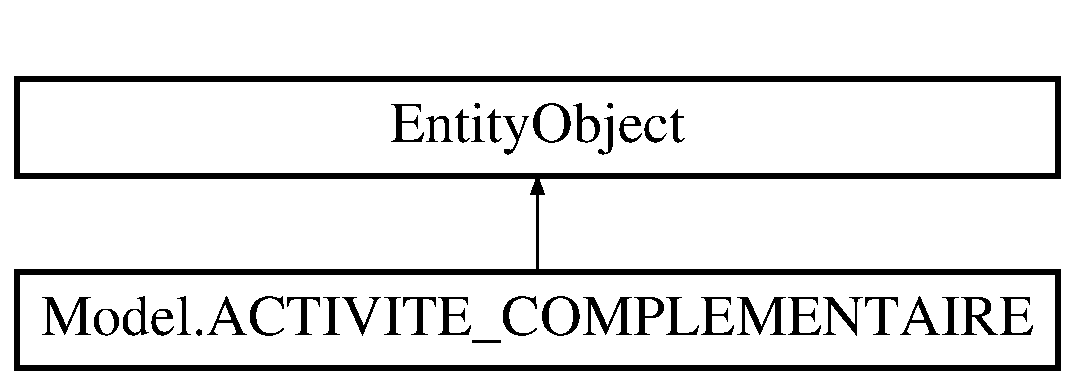
\includegraphics[height=2.000000cm]{class_model_1_1_a_c_t_i_v_i_t_e___c_o_m_p_l_e_m_e_n_t_a_i_r_e}
\end{center}
\end{figure}
\subsection*{Static Public Member Functions}
\begin{DoxyCompactItemize}
\item 
static \hyperlink{class_model_1_1_a_c_t_i_v_i_t_e___c_o_m_p_l_e_m_e_n_t_a_i_r_e}{A\-C\-T\-I\-V\-I\-T\-E\-\_\-\-C\-O\-M\-P\-L\-E\-M\-E\-N\-T\-A\-I\-R\-E} \hyperlink{class_model_1_1_a_c_t_i_v_i_t_e___c_o_m_p_l_e_m_e_n_t_a_i_r_e_a24ea0e9c3b1ed384f688ff056f124063}{Create\-A\-C\-T\-I\-V\-I\-T\-E\-\_\-\-C\-O\-M\-P\-L\-E\-M\-E\-N\-T\-A\-I\-R\-E} (global\-::\-System.\-Int32 \hyperlink{class_model_1_1_a_c_t_i_v_i_t_e___c_o_m_p_l_e_m_e_n_t_a_i_r_e_a52209b9d343c9c1f6a0d6fd06ee11caf}{num\-\_\-act}, global\-::\-System.\-String \hyperlink{class_model_1_1_a_c_t_i_v_i_t_e___c_o_m_p_l_e_m_e_n_t_a_i_r_e_ac31dc74da88e2bba3a7878e0de1da922}{theme\-\_\-act}, global\-::\-System.\-String \hyperlink{class_model_1_1_a_c_t_i_v_i_t_e___c_o_m_p_l_e_m_e_n_t_a_i_r_e_acc59469c7bb41fc47d357b1352b6e9bc}{montant\-\_\-act}, global\-::\-System.\-Date\-Time \hyperlink{class_model_1_1_a_c_t_i_v_i_t_e___c_o_m_p_l_e_m_e_n_t_a_i_r_e_aacbeaa9cd3bfc61485c1ee7164d7a424}{date\-\_\-act}, global\-::\-System.\-String \hyperlink{class_model_1_1_a_c_t_i_v_i_t_e___c_o_m_p_l_e_m_e_n_t_a_i_r_e_a730e1eac8f9fafbb0f48672688609f5e}{lieu\-\_\-act})
\begin{DoxyCompactList}\small\item\em Créez un nouvel objet \hyperlink{class_model_1_1_a_c_t_i_v_i_t_e___c_o_m_p_l_e_m_e_n_t_a_i_r_e}{A\-C\-T\-I\-V\-I\-T\-E\-\_\-\-C\-O\-M\-P\-L\-E\-M\-E\-N\-T\-A\-I\-R\-E}. \end{DoxyCompactList}\end{DoxyCompactItemize}
\subsection*{Properties}
\begin{DoxyCompactItemize}
\item 
global\-::\-System.\-Int32 \hyperlink{class_model_1_1_a_c_t_i_v_i_t_e___c_o_m_p_l_e_m_e_n_t_a_i_r_e_a52209b9d343c9c1f6a0d6fd06ee11caf}{num\-\_\-act}\hspace{0.3cm}{\ttfamily  \mbox{[}get, set\mbox{]}}
\begin{DoxyCompactList}\small\item\em Aucune documentation sur les métadonnées n'est disponible. \end{DoxyCompactList}\item 
Nullable$<$ global\-::\-System.\-Int32 $>$ \hyperlink{class_model_1_1_a_c_t_i_v_i_t_e___c_o_m_p_l_e_m_e_n_t_a_i_r_e_a68164855e37062f280439aece991e95f}{matricule\-\_\-col\-\_\-act}\hspace{0.3cm}{\ttfamily  \mbox{[}get, set\mbox{]}}
\begin{DoxyCompactList}\small\item\em Aucune documentation sur les métadonnées n'est disponible. \end{DoxyCompactList}\item 
global\-::\-System.\-String \hyperlink{class_model_1_1_a_c_t_i_v_i_t_e___c_o_m_p_l_e_m_e_n_t_a_i_r_e_ac31dc74da88e2bba3a7878e0de1da922}{theme\-\_\-act}\hspace{0.3cm}{\ttfamily  \mbox{[}get, set\mbox{]}}
\begin{DoxyCompactList}\small\item\em Aucune documentation sur les métadonnées n'est disponible. \end{DoxyCompactList}\item 
global\-::\-System.\-String \hyperlink{class_model_1_1_a_c_t_i_v_i_t_e___c_o_m_p_l_e_m_e_n_t_a_i_r_e_acc59469c7bb41fc47d357b1352b6e9bc}{montant\-\_\-act}\hspace{0.3cm}{\ttfamily  \mbox{[}get, set\mbox{]}}
\begin{DoxyCompactList}\small\item\em Aucune documentation sur les métadonnées n'est disponible. \end{DoxyCompactList}\item 
global\-::\-System.\-Date\-Time \hyperlink{class_model_1_1_a_c_t_i_v_i_t_e___c_o_m_p_l_e_m_e_n_t_a_i_r_e_aacbeaa9cd3bfc61485c1ee7164d7a424}{date\-\_\-act}\hspace{0.3cm}{\ttfamily  \mbox{[}get, set\mbox{]}}
\begin{DoxyCompactList}\small\item\em Aucune documentation sur les métadonnées n'est disponible. \end{DoxyCompactList}\item 
global\-::\-System.\-String \hyperlink{class_model_1_1_a_c_t_i_v_i_t_e___c_o_m_p_l_e_m_e_n_t_a_i_r_e_a730e1eac8f9fafbb0f48672688609f5e}{lieu\-\_\-act}\hspace{0.3cm}{\ttfamily  \mbox{[}get, set\mbox{]}}
\begin{DoxyCompactList}\small\item\em Aucune documentation sur les métadonnées n'est disponible. \end{DoxyCompactList}\item 
\hyperlink{class_model_1_1_c_o_l_l_a_b_o_r_a_t_e_u_r}{C\-O\-L\-L\-A\-B\-O\-R\-A\-T\-E\-U\-R} \hyperlink{class_model_1_1_a_c_t_i_v_i_t_e___c_o_m_p_l_e_m_e_n_t_a_i_r_e_a0406f3c3e100219c6474603c5c5a6841}{C\-O\-L\-L\-A\-B\-O\-R\-A\-T\-E\-U\-R}\hspace{0.3cm}{\ttfamily  \mbox{[}get, set\mbox{]}}
\begin{DoxyCompactList}\small\item\em Aucune documentation sur les métadonnées n'est disponible. \end{DoxyCompactList}\item 
Entity\-Reference$<$ \hyperlink{class_model_1_1_c_o_l_l_a_b_o_r_a_t_e_u_r}{C\-O\-L\-L\-A\-B\-O\-R\-A\-T\-E\-U\-R} $>$ \hyperlink{class_model_1_1_a_c_t_i_v_i_t_e___c_o_m_p_l_e_m_e_n_t_a_i_r_e_af0414ca6acf19af2edf4faf25b69e347}{C\-O\-L\-L\-A\-B\-O\-R\-A\-T\-E\-U\-R\-Reference}\hspace{0.3cm}{\ttfamily  \mbox{[}get, set\mbox{]}}
\begin{DoxyCompactList}\small\item\em Aucune documentation sur les métadonnées n'est disponible. \end{DoxyCompactList}\item 
Entity\-Collection$<$ \hyperlink{class_model_1_1_c_o_l_l_a_b_o_r_a_t_e_u_r}{C\-O\-L\-L\-A\-B\-O\-R\-A\-T\-E\-U\-R} $>$ \hyperlink{class_model_1_1_a_c_t_i_v_i_t_e___c_o_m_p_l_e_m_e_n_t_a_i_r_e_a5060b22b62f8398491d89da890ae8ce0}{C\-O\-L\-L\-A\-B\-O\-R\-A\-T\-E\-U\-R1}\hspace{0.3cm}{\ttfamily  \mbox{[}get, set\mbox{]}}
\begin{DoxyCompactList}\small\item\em Aucune documentation sur les métadonnées n'est disponible. \end{DoxyCompactList}\item 
Entity\-Collection$<$ \hyperlink{class_model_1_1_p_r_a_t_i_c_i_e_n}{P\-R\-A\-T\-I\-C\-I\-E\-N} $>$ \hyperlink{class_model_1_1_a_c_t_i_v_i_t_e___c_o_m_p_l_e_m_e_n_t_a_i_r_e_a0d894abf403b688a6fb3058c1861e382}{P\-R\-A\-T\-I\-C\-I\-E\-N}\hspace{0.3cm}{\ttfamily  \mbox{[}get, set\mbox{]}}
\begin{DoxyCompactList}\small\item\em Aucune documentation sur les métadonnées n'est disponible. \end{DoxyCompactList}\end{DoxyCompactItemize}


\subsection{Detailed Description}
Aucune documentation sur les métadonnées n'est disponible. 



\subsection{Member Function Documentation}
\hypertarget{class_model_1_1_a_c_t_i_v_i_t_e___c_o_m_p_l_e_m_e_n_t_a_i_r_e_a24ea0e9c3b1ed384f688ff056f124063}{\index{Model\-::\-A\-C\-T\-I\-V\-I\-T\-E\-\_\-\-C\-O\-M\-P\-L\-E\-M\-E\-N\-T\-A\-I\-R\-E@{Model\-::\-A\-C\-T\-I\-V\-I\-T\-E\-\_\-\-C\-O\-M\-P\-L\-E\-M\-E\-N\-T\-A\-I\-R\-E}!Create\-A\-C\-T\-I\-V\-I\-T\-E\-\_\-\-C\-O\-M\-P\-L\-E\-M\-E\-N\-T\-A\-I\-R\-E@{Create\-A\-C\-T\-I\-V\-I\-T\-E\-\_\-\-C\-O\-M\-P\-L\-E\-M\-E\-N\-T\-A\-I\-R\-E}}
\index{Create\-A\-C\-T\-I\-V\-I\-T\-E\-\_\-\-C\-O\-M\-P\-L\-E\-M\-E\-N\-T\-A\-I\-R\-E@{Create\-A\-C\-T\-I\-V\-I\-T\-E\-\_\-\-C\-O\-M\-P\-L\-E\-M\-E\-N\-T\-A\-I\-R\-E}!Model::ACTIVITE_COMPLEMENTAIRE@{Model\-::\-A\-C\-T\-I\-V\-I\-T\-E\-\_\-\-C\-O\-M\-P\-L\-E\-M\-E\-N\-T\-A\-I\-R\-E}}
\subsubsection[{Create\-A\-C\-T\-I\-V\-I\-T\-E\-\_\-\-C\-O\-M\-P\-L\-E\-M\-E\-N\-T\-A\-I\-R\-E}]{\setlength{\rightskip}{0pt plus 5cm}static {\bf A\-C\-T\-I\-V\-I\-T\-E\-\_\-\-C\-O\-M\-P\-L\-E\-M\-E\-N\-T\-A\-I\-R\-E} Model.\-A\-C\-T\-I\-V\-I\-T\-E\-\_\-\-C\-O\-M\-P\-L\-E\-M\-E\-N\-T\-A\-I\-R\-E.\-Create\-A\-C\-T\-I\-V\-I\-T\-E\-\_\-\-C\-O\-M\-P\-L\-E\-M\-E\-N\-T\-A\-I\-R\-E (
\begin{DoxyParamCaption}
\item[{global\-::\-System.\-Int32}]{num\-\_\-act, }
\item[{global\-::\-System.\-String}]{theme\-\_\-act, }
\item[{global\-::\-System.\-String}]{montant\-\_\-act, }
\item[{global\-::\-System.\-Date\-Time}]{date\-\_\-act, }
\item[{global\-::\-System.\-String}]{lieu\-\_\-act}
\end{DoxyParamCaption}
)\hspace{0.3cm}{\ttfamily [static]}}}\label{class_model_1_1_a_c_t_i_v_i_t_e___c_o_m_p_l_e_m_e_n_t_a_i_r_e_a24ea0e9c3b1ed384f688ff056f124063}


Créez un nouvel objet \hyperlink{class_model_1_1_a_c_t_i_v_i_t_e___c_o_m_p_l_e_m_e_n_t_a_i_r_e}{A\-C\-T\-I\-V\-I\-T\-E\-\_\-\-C\-O\-M\-P\-L\-E\-M\-E\-N\-T\-A\-I\-R\-E}. 


\begin{DoxyParams}{Parameters}
{\em num\-\_\-act} & Valeur initiale de la propriété num\-\_\-act.\\
\hline
{\em theme\-\_\-act} & Valeur initiale de la propriété theme\-\_\-act.\\
\hline
{\em montant\-\_\-act} & Valeur initiale de la propriété montant\-\_\-act.\\
\hline
{\em date\-\_\-act} & Valeur initiale de la propriété date\-\_\-act.\\
\hline
{\em lieu\-\_\-act} & Valeur initiale de la propriété lieu\-\_\-act.\\
\hline
\end{DoxyParams}


\subsection{Property Documentation}
\hypertarget{class_model_1_1_a_c_t_i_v_i_t_e___c_o_m_p_l_e_m_e_n_t_a_i_r_e_a0406f3c3e100219c6474603c5c5a6841}{\index{Model\-::\-A\-C\-T\-I\-V\-I\-T\-E\-\_\-\-C\-O\-M\-P\-L\-E\-M\-E\-N\-T\-A\-I\-R\-E@{Model\-::\-A\-C\-T\-I\-V\-I\-T\-E\-\_\-\-C\-O\-M\-P\-L\-E\-M\-E\-N\-T\-A\-I\-R\-E}!C\-O\-L\-L\-A\-B\-O\-R\-A\-T\-E\-U\-R@{C\-O\-L\-L\-A\-B\-O\-R\-A\-T\-E\-U\-R}}
\index{C\-O\-L\-L\-A\-B\-O\-R\-A\-T\-E\-U\-R@{C\-O\-L\-L\-A\-B\-O\-R\-A\-T\-E\-U\-R}!Model::ACTIVITE_COMPLEMENTAIRE@{Model\-::\-A\-C\-T\-I\-V\-I\-T\-E\-\_\-\-C\-O\-M\-P\-L\-E\-M\-E\-N\-T\-A\-I\-R\-E}}
\subsubsection[{C\-O\-L\-L\-A\-B\-O\-R\-A\-T\-E\-U\-R}]{\setlength{\rightskip}{0pt plus 5cm}{\bf C\-O\-L\-L\-A\-B\-O\-R\-A\-T\-E\-U\-R} Model.\-A\-C\-T\-I\-V\-I\-T\-E\-\_\-\-C\-O\-M\-P\-L\-E\-M\-E\-N\-T\-A\-I\-R\-E.\-C\-O\-L\-L\-A\-B\-O\-R\-A\-T\-E\-U\-R\hspace{0.3cm}{\ttfamily [get]}, {\ttfamily [set]}}}\label{class_model_1_1_a_c_t_i_v_i_t_e___c_o_m_p_l_e_m_e_n_t_a_i_r_e_a0406f3c3e100219c6474603c5c5a6841}


Aucune documentation sur les métadonnées n'est disponible. 

\hypertarget{class_model_1_1_a_c_t_i_v_i_t_e___c_o_m_p_l_e_m_e_n_t_a_i_r_e_a5060b22b62f8398491d89da890ae8ce0}{\index{Model\-::\-A\-C\-T\-I\-V\-I\-T\-E\-\_\-\-C\-O\-M\-P\-L\-E\-M\-E\-N\-T\-A\-I\-R\-E@{Model\-::\-A\-C\-T\-I\-V\-I\-T\-E\-\_\-\-C\-O\-M\-P\-L\-E\-M\-E\-N\-T\-A\-I\-R\-E}!C\-O\-L\-L\-A\-B\-O\-R\-A\-T\-E\-U\-R1@{C\-O\-L\-L\-A\-B\-O\-R\-A\-T\-E\-U\-R1}}
\index{C\-O\-L\-L\-A\-B\-O\-R\-A\-T\-E\-U\-R1@{C\-O\-L\-L\-A\-B\-O\-R\-A\-T\-E\-U\-R1}!Model::ACTIVITE_COMPLEMENTAIRE@{Model\-::\-A\-C\-T\-I\-V\-I\-T\-E\-\_\-\-C\-O\-M\-P\-L\-E\-M\-E\-N\-T\-A\-I\-R\-E}}
\subsubsection[{C\-O\-L\-L\-A\-B\-O\-R\-A\-T\-E\-U\-R1}]{\setlength{\rightskip}{0pt plus 5cm}Entity\-Collection$<${\bf C\-O\-L\-L\-A\-B\-O\-R\-A\-T\-E\-U\-R}$>$ Model.\-A\-C\-T\-I\-V\-I\-T\-E\-\_\-\-C\-O\-M\-P\-L\-E\-M\-E\-N\-T\-A\-I\-R\-E.\-C\-O\-L\-L\-A\-B\-O\-R\-A\-T\-E\-U\-R1\hspace{0.3cm}{\ttfamily [get]}, {\ttfamily [set]}}}\label{class_model_1_1_a_c_t_i_v_i_t_e___c_o_m_p_l_e_m_e_n_t_a_i_r_e_a5060b22b62f8398491d89da890ae8ce0}


Aucune documentation sur les métadonnées n'est disponible. 

\hypertarget{class_model_1_1_a_c_t_i_v_i_t_e___c_o_m_p_l_e_m_e_n_t_a_i_r_e_af0414ca6acf19af2edf4faf25b69e347}{\index{Model\-::\-A\-C\-T\-I\-V\-I\-T\-E\-\_\-\-C\-O\-M\-P\-L\-E\-M\-E\-N\-T\-A\-I\-R\-E@{Model\-::\-A\-C\-T\-I\-V\-I\-T\-E\-\_\-\-C\-O\-M\-P\-L\-E\-M\-E\-N\-T\-A\-I\-R\-E}!C\-O\-L\-L\-A\-B\-O\-R\-A\-T\-E\-U\-R\-Reference@{C\-O\-L\-L\-A\-B\-O\-R\-A\-T\-E\-U\-R\-Reference}}
\index{C\-O\-L\-L\-A\-B\-O\-R\-A\-T\-E\-U\-R\-Reference@{C\-O\-L\-L\-A\-B\-O\-R\-A\-T\-E\-U\-R\-Reference}!Model::ACTIVITE_COMPLEMENTAIRE@{Model\-::\-A\-C\-T\-I\-V\-I\-T\-E\-\_\-\-C\-O\-M\-P\-L\-E\-M\-E\-N\-T\-A\-I\-R\-E}}
\subsubsection[{C\-O\-L\-L\-A\-B\-O\-R\-A\-T\-E\-U\-R\-Reference}]{\setlength{\rightskip}{0pt plus 5cm}Entity\-Reference$<${\bf C\-O\-L\-L\-A\-B\-O\-R\-A\-T\-E\-U\-R}$>$ Model.\-A\-C\-T\-I\-V\-I\-T\-E\-\_\-\-C\-O\-M\-P\-L\-E\-M\-E\-N\-T\-A\-I\-R\-E.\-C\-O\-L\-L\-A\-B\-O\-R\-A\-T\-E\-U\-R\-Reference\hspace{0.3cm}{\ttfamily [get]}, {\ttfamily [set]}}}\label{class_model_1_1_a_c_t_i_v_i_t_e___c_o_m_p_l_e_m_e_n_t_a_i_r_e_af0414ca6acf19af2edf4faf25b69e347}


Aucune documentation sur les métadonnées n'est disponible. 

\hypertarget{class_model_1_1_a_c_t_i_v_i_t_e___c_o_m_p_l_e_m_e_n_t_a_i_r_e_aacbeaa9cd3bfc61485c1ee7164d7a424}{\index{Model\-::\-A\-C\-T\-I\-V\-I\-T\-E\-\_\-\-C\-O\-M\-P\-L\-E\-M\-E\-N\-T\-A\-I\-R\-E@{Model\-::\-A\-C\-T\-I\-V\-I\-T\-E\-\_\-\-C\-O\-M\-P\-L\-E\-M\-E\-N\-T\-A\-I\-R\-E}!date\-\_\-act@{date\-\_\-act}}
\index{date\-\_\-act@{date\-\_\-act}!Model::ACTIVITE_COMPLEMENTAIRE@{Model\-::\-A\-C\-T\-I\-V\-I\-T\-E\-\_\-\-C\-O\-M\-P\-L\-E\-M\-E\-N\-T\-A\-I\-R\-E}}
\subsubsection[{date\-\_\-act}]{\setlength{\rightskip}{0pt plus 5cm}global.\-System.\-Date\-Time Model.\-A\-C\-T\-I\-V\-I\-T\-E\-\_\-\-C\-O\-M\-P\-L\-E\-M\-E\-N\-T\-A\-I\-R\-E.\-date\-\_\-act\hspace{0.3cm}{\ttfamily [get]}, {\ttfamily [set]}}}\label{class_model_1_1_a_c_t_i_v_i_t_e___c_o_m_p_l_e_m_e_n_t_a_i_r_e_aacbeaa9cd3bfc61485c1ee7164d7a424}


Aucune documentation sur les métadonnées n'est disponible. 

\hypertarget{class_model_1_1_a_c_t_i_v_i_t_e___c_o_m_p_l_e_m_e_n_t_a_i_r_e_a730e1eac8f9fafbb0f48672688609f5e}{\index{Model\-::\-A\-C\-T\-I\-V\-I\-T\-E\-\_\-\-C\-O\-M\-P\-L\-E\-M\-E\-N\-T\-A\-I\-R\-E@{Model\-::\-A\-C\-T\-I\-V\-I\-T\-E\-\_\-\-C\-O\-M\-P\-L\-E\-M\-E\-N\-T\-A\-I\-R\-E}!lieu\-\_\-act@{lieu\-\_\-act}}
\index{lieu\-\_\-act@{lieu\-\_\-act}!Model::ACTIVITE_COMPLEMENTAIRE@{Model\-::\-A\-C\-T\-I\-V\-I\-T\-E\-\_\-\-C\-O\-M\-P\-L\-E\-M\-E\-N\-T\-A\-I\-R\-E}}
\subsubsection[{lieu\-\_\-act}]{\setlength{\rightskip}{0pt plus 5cm}global.\-System.\-String Model.\-A\-C\-T\-I\-V\-I\-T\-E\-\_\-\-C\-O\-M\-P\-L\-E\-M\-E\-N\-T\-A\-I\-R\-E.\-lieu\-\_\-act\hspace{0.3cm}{\ttfamily [get]}, {\ttfamily [set]}}}\label{class_model_1_1_a_c_t_i_v_i_t_e___c_o_m_p_l_e_m_e_n_t_a_i_r_e_a730e1eac8f9fafbb0f48672688609f5e}


Aucune documentation sur les métadonnées n'est disponible. 

\hypertarget{class_model_1_1_a_c_t_i_v_i_t_e___c_o_m_p_l_e_m_e_n_t_a_i_r_e_a68164855e37062f280439aece991e95f}{\index{Model\-::\-A\-C\-T\-I\-V\-I\-T\-E\-\_\-\-C\-O\-M\-P\-L\-E\-M\-E\-N\-T\-A\-I\-R\-E@{Model\-::\-A\-C\-T\-I\-V\-I\-T\-E\-\_\-\-C\-O\-M\-P\-L\-E\-M\-E\-N\-T\-A\-I\-R\-E}!matricule\-\_\-col\-\_\-act@{matricule\-\_\-col\-\_\-act}}
\index{matricule\-\_\-col\-\_\-act@{matricule\-\_\-col\-\_\-act}!Model::ACTIVITE_COMPLEMENTAIRE@{Model\-::\-A\-C\-T\-I\-V\-I\-T\-E\-\_\-\-C\-O\-M\-P\-L\-E\-M\-E\-N\-T\-A\-I\-R\-E}}
\subsubsection[{matricule\-\_\-col\-\_\-act}]{\setlength{\rightskip}{0pt plus 5cm}Nullable$<$global.\-System.\-Int32$>$ Model.\-A\-C\-T\-I\-V\-I\-T\-E\-\_\-\-C\-O\-M\-P\-L\-E\-M\-E\-N\-T\-A\-I\-R\-E.\-matricule\-\_\-col\-\_\-act\hspace{0.3cm}{\ttfamily [get]}, {\ttfamily [set]}}}\label{class_model_1_1_a_c_t_i_v_i_t_e___c_o_m_p_l_e_m_e_n_t_a_i_r_e_a68164855e37062f280439aece991e95f}


Aucune documentation sur les métadonnées n'est disponible. 

\hypertarget{class_model_1_1_a_c_t_i_v_i_t_e___c_o_m_p_l_e_m_e_n_t_a_i_r_e_acc59469c7bb41fc47d357b1352b6e9bc}{\index{Model\-::\-A\-C\-T\-I\-V\-I\-T\-E\-\_\-\-C\-O\-M\-P\-L\-E\-M\-E\-N\-T\-A\-I\-R\-E@{Model\-::\-A\-C\-T\-I\-V\-I\-T\-E\-\_\-\-C\-O\-M\-P\-L\-E\-M\-E\-N\-T\-A\-I\-R\-E}!montant\-\_\-act@{montant\-\_\-act}}
\index{montant\-\_\-act@{montant\-\_\-act}!Model::ACTIVITE_COMPLEMENTAIRE@{Model\-::\-A\-C\-T\-I\-V\-I\-T\-E\-\_\-\-C\-O\-M\-P\-L\-E\-M\-E\-N\-T\-A\-I\-R\-E}}
\subsubsection[{montant\-\_\-act}]{\setlength{\rightskip}{0pt plus 5cm}global.\-System.\-String Model.\-A\-C\-T\-I\-V\-I\-T\-E\-\_\-\-C\-O\-M\-P\-L\-E\-M\-E\-N\-T\-A\-I\-R\-E.\-montant\-\_\-act\hspace{0.3cm}{\ttfamily [get]}, {\ttfamily [set]}}}\label{class_model_1_1_a_c_t_i_v_i_t_e___c_o_m_p_l_e_m_e_n_t_a_i_r_e_acc59469c7bb41fc47d357b1352b6e9bc}


Aucune documentation sur les métadonnées n'est disponible. 

\hypertarget{class_model_1_1_a_c_t_i_v_i_t_e___c_o_m_p_l_e_m_e_n_t_a_i_r_e_a52209b9d343c9c1f6a0d6fd06ee11caf}{\index{Model\-::\-A\-C\-T\-I\-V\-I\-T\-E\-\_\-\-C\-O\-M\-P\-L\-E\-M\-E\-N\-T\-A\-I\-R\-E@{Model\-::\-A\-C\-T\-I\-V\-I\-T\-E\-\_\-\-C\-O\-M\-P\-L\-E\-M\-E\-N\-T\-A\-I\-R\-E}!num\-\_\-act@{num\-\_\-act}}
\index{num\-\_\-act@{num\-\_\-act}!Model::ACTIVITE_COMPLEMENTAIRE@{Model\-::\-A\-C\-T\-I\-V\-I\-T\-E\-\_\-\-C\-O\-M\-P\-L\-E\-M\-E\-N\-T\-A\-I\-R\-E}}
\subsubsection[{num\-\_\-act}]{\setlength{\rightskip}{0pt plus 5cm}global.\-System.\-Int32 Model.\-A\-C\-T\-I\-V\-I\-T\-E\-\_\-\-C\-O\-M\-P\-L\-E\-M\-E\-N\-T\-A\-I\-R\-E.\-num\-\_\-act\hspace{0.3cm}{\ttfamily [get]}, {\ttfamily [set]}}}\label{class_model_1_1_a_c_t_i_v_i_t_e___c_o_m_p_l_e_m_e_n_t_a_i_r_e_a52209b9d343c9c1f6a0d6fd06ee11caf}


Aucune documentation sur les métadonnées n'est disponible. 

\hypertarget{class_model_1_1_a_c_t_i_v_i_t_e___c_o_m_p_l_e_m_e_n_t_a_i_r_e_a0d894abf403b688a6fb3058c1861e382}{\index{Model\-::\-A\-C\-T\-I\-V\-I\-T\-E\-\_\-\-C\-O\-M\-P\-L\-E\-M\-E\-N\-T\-A\-I\-R\-E@{Model\-::\-A\-C\-T\-I\-V\-I\-T\-E\-\_\-\-C\-O\-M\-P\-L\-E\-M\-E\-N\-T\-A\-I\-R\-E}!P\-R\-A\-T\-I\-C\-I\-E\-N@{P\-R\-A\-T\-I\-C\-I\-E\-N}}
\index{P\-R\-A\-T\-I\-C\-I\-E\-N@{P\-R\-A\-T\-I\-C\-I\-E\-N}!Model::ACTIVITE_COMPLEMENTAIRE@{Model\-::\-A\-C\-T\-I\-V\-I\-T\-E\-\_\-\-C\-O\-M\-P\-L\-E\-M\-E\-N\-T\-A\-I\-R\-E}}
\subsubsection[{P\-R\-A\-T\-I\-C\-I\-E\-N}]{\setlength{\rightskip}{0pt plus 5cm}Entity\-Collection$<${\bf P\-R\-A\-T\-I\-C\-I\-E\-N}$>$ Model.\-A\-C\-T\-I\-V\-I\-T\-E\-\_\-\-C\-O\-M\-P\-L\-E\-M\-E\-N\-T\-A\-I\-R\-E.\-P\-R\-A\-T\-I\-C\-I\-E\-N\hspace{0.3cm}{\ttfamily [get]}, {\ttfamily [set]}}}\label{class_model_1_1_a_c_t_i_v_i_t_e___c_o_m_p_l_e_m_e_n_t_a_i_r_e_a0d894abf403b688a6fb3058c1861e382}


Aucune documentation sur les métadonnées n'est disponible. 

\hypertarget{class_model_1_1_a_c_t_i_v_i_t_e___c_o_m_p_l_e_m_e_n_t_a_i_r_e_ac31dc74da88e2bba3a7878e0de1da922}{\index{Model\-::\-A\-C\-T\-I\-V\-I\-T\-E\-\_\-\-C\-O\-M\-P\-L\-E\-M\-E\-N\-T\-A\-I\-R\-E@{Model\-::\-A\-C\-T\-I\-V\-I\-T\-E\-\_\-\-C\-O\-M\-P\-L\-E\-M\-E\-N\-T\-A\-I\-R\-E}!theme\-\_\-act@{theme\-\_\-act}}
\index{theme\-\_\-act@{theme\-\_\-act}!Model::ACTIVITE_COMPLEMENTAIRE@{Model\-::\-A\-C\-T\-I\-V\-I\-T\-E\-\_\-\-C\-O\-M\-P\-L\-E\-M\-E\-N\-T\-A\-I\-R\-E}}
\subsubsection[{theme\-\_\-act}]{\setlength{\rightskip}{0pt plus 5cm}global.\-System.\-String Model.\-A\-C\-T\-I\-V\-I\-T\-E\-\_\-\-C\-O\-M\-P\-L\-E\-M\-E\-N\-T\-A\-I\-R\-E.\-theme\-\_\-act\hspace{0.3cm}{\ttfamily [get]}, {\ttfamily [set]}}}\label{class_model_1_1_a_c_t_i_v_i_t_e___c_o_m_p_l_e_m_e_n_t_a_i_r_e_ac31dc74da88e2bba3a7878e0de1da922}


Aucune documentation sur les métadonnées n'est disponible. 



The documentation for this class was generated from the following file\-:\begin{DoxyCompactItemize}
\item 
C\-:/\-Users/dju/\-Documents/\-Visual Studio 2012/\-Projects/\-P\-P\-E/\-P\-P\-E3/\-Model/\hyperlink{_model_bdd_sio_8_designer_8cs}{Model\-Bdd\-Sio.\-Designer.\-cs}\end{DoxyCompactItemize}

\hypertarget{class_wpf_application_1_1_app}{\section{Wpf\-Application.\-App Class Reference}
\label{class_wpf_application_1_1_app}\index{Wpf\-Application.\-App@{Wpf\-Application.\-App}}
}


Logique d'interaction pour App.\-xaml  


Inheritance diagram for Wpf\-Application.\-App\-:\begin{figure}[H]
\begin{center}
\leavevmode
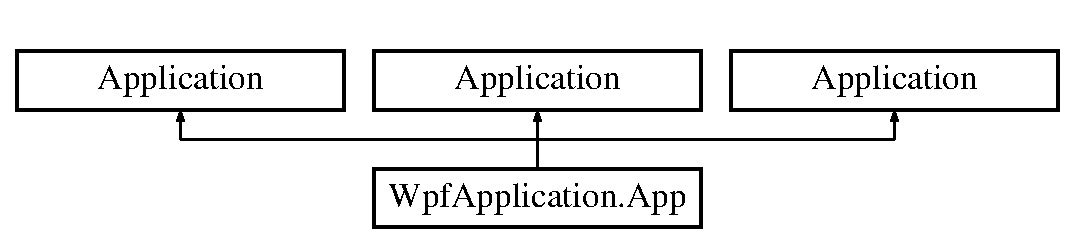
\includegraphics[height=2.000000cm]{class_wpf_application_1_1_app}
\end{center}
\end{figure}
\subsection*{Public Member Functions}
\begin{DoxyCompactItemize}
\item 
void \hyperlink{class_wpf_application_1_1_app_a85afd6d15ea6481274dd01c8f43afba0}{Initialize\-Component} ()
\begin{DoxyCompactList}\small\item\em Initialize\-Component \end{DoxyCompactList}\item 
void \hyperlink{class_wpf_application_1_1_app_a85afd6d15ea6481274dd01c8f43afba0}{Initialize\-Component} ()
\begin{DoxyCompactList}\small\item\em Initialize\-Component \end{DoxyCompactList}\end{DoxyCompactItemize}
\subsection*{Static Public Member Functions}
\begin{DoxyCompactItemize}
\item 
static void \hyperlink{class_wpf_application_1_1_app_a5495f372717728281b455336a48c5d4e}{Main} ()
\begin{DoxyCompactList}\small\item\em Application Entry Point. \end{DoxyCompactList}\item 
static void \hyperlink{class_wpf_application_1_1_app_a5495f372717728281b455336a48c5d4e}{Main} ()
\begin{DoxyCompactList}\small\item\em Application Entry Point. \end{DoxyCompactList}\end{DoxyCompactItemize}


\subsection{Detailed Description}
Logique d'interaction pour App.\-xaml 

\hyperlink{class_wpf_application_1_1_app}{App} 

\subsection{Member Function Documentation}
\hypertarget{class_wpf_application_1_1_app_a85afd6d15ea6481274dd01c8f43afba0}{\index{Wpf\-Application\-::\-App@{Wpf\-Application\-::\-App}!Initialize\-Component@{Initialize\-Component}}
\index{Initialize\-Component@{Initialize\-Component}!WpfApplication::App@{Wpf\-Application\-::\-App}}
\subsubsection[{Initialize\-Component}]{\setlength{\rightskip}{0pt plus 5cm}void Wpf\-Application.\-App.\-Initialize\-Component (
\begin{DoxyParamCaption}
{}
\end{DoxyParamCaption}
)}}\label{class_wpf_application_1_1_app_a85afd6d15ea6481274dd01c8f43afba0}


Initialize\-Component 

\hypertarget{class_wpf_application_1_1_app_a85afd6d15ea6481274dd01c8f43afba0}{\index{Wpf\-Application\-::\-App@{Wpf\-Application\-::\-App}!Initialize\-Component@{Initialize\-Component}}
\index{Initialize\-Component@{Initialize\-Component}!WpfApplication::App@{Wpf\-Application\-::\-App}}
\subsubsection[{Initialize\-Component}]{\setlength{\rightskip}{0pt plus 5cm}void Wpf\-Application.\-App.\-Initialize\-Component (
\begin{DoxyParamCaption}
{}
\end{DoxyParamCaption}
)}}\label{class_wpf_application_1_1_app_a85afd6d15ea6481274dd01c8f43afba0}


Initialize\-Component 

\hypertarget{class_wpf_application_1_1_app_a5495f372717728281b455336a48c5d4e}{\index{Wpf\-Application\-::\-App@{Wpf\-Application\-::\-App}!Main@{Main}}
\index{Main@{Main}!WpfApplication::App@{Wpf\-Application\-::\-App}}
\subsubsection[{Main}]{\setlength{\rightskip}{0pt plus 5cm}static void Wpf\-Application.\-App.\-Main (
\begin{DoxyParamCaption}
{}
\end{DoxyParamCaption}
)\hspace{0.3cm}{\ttfamily [static]}}}\label{class_wpf_application_1_1_app_a5495f372717728281b455336a48c5d4e}


Application Entry Point. 

\hypertarget{class_wpf_application_1_1_app_a5495f372717728281b455336a48c5d4e}{\index{Wpf\-Application\-::\-App@{Wpf\-Application\-::\-App}!Main@{Main}}
\index{Main@{Main}!WpfApplication::App@{Wpf\-Application\-::\-App}}
\subsubsection[{Main}]{\setlength{\rightskip}{0pt plus 5cm}static void Wpf\-Application.\-App.\-Main (
\begin{DoxyParamCaption}
{}
\end{DoxyParamCaption}
)\hspace{0.3cm}{\ttfamily [static]}}}\label{class_wpf_application_1_1_app_a5495f372717728281b455336a48c5d4e}


Application Entry Point. 



The documentation for this class was generated from the following files\-:\begin{DoxyCompactItemize}
\item 
C\-:/\-Users/dju/\-Documents/\-Visual Studio 2012/\-Projects/\-P\-P\-E/\-P\-P\-E3/\-Wpf\-Application/\hyperlink{_app_8xaml_8cs}{App.\-xaml.\-cs}\item 
C\-:/\-Users/dju/\-Documents/\-Visual Studio 2012/\-Projects/\-P\-P\-E/\-P\-P\-E3/\-Wpf\-Application/obj/\-Debug/\hyperlink{_app_8g_8cs}{App.\-g.\-cs}\item 
C\-:/\-Users/dju/\-Documents/\-Visual Studio 2012/\-Projects/\-P\-P\-E/\-P\-P\-E3/\-Wpf\-Application/obj/\-Debug/\hyperlink{_app_8g_8i_8cs}{App.\-g.\-i.\-cs}\end{DoxyCompactItemize}

\hypertarget{class_model_1_1_a_v_o_i_r1}{\section{Model.\-A\-V\-O\-I\-R1 Class Reference}
\label{class_model_1_1_a_v_o_i_r1}\index{Model.\-A\-V\-O\-I\-R1@{Model.\-A\-V\-O\-I\-R1}}
}


Aucune documentation sur les métadonnées n'est disponible.  


Inheritance diagram for Model.\-A\-V\-O\-I\-R1\-:\begin{figure}[H]
\begin{center}
\leavevmode
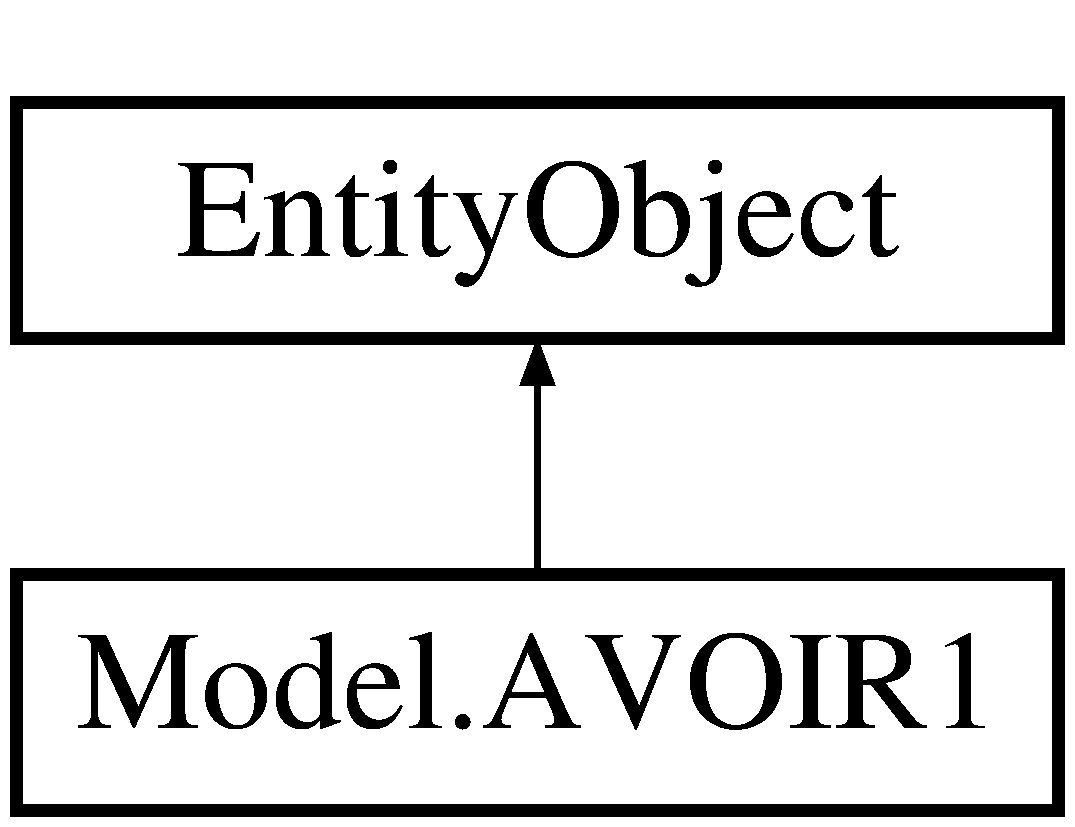
\includegraphics[height=2.000000cm]{class_model_1_1_a_v_o_i_r1}
\end{center}
\end{figure}
\subsection*{Static Public Member Functions}
\begin{DoxyCompactItemize}
\item 
static \hyperlink{class_model_1_1_a_v_o_i_r1}{A\-V\-O\-I\-R1} \hyperlink{class_model_1_1_a_v_o_i_r1_a64ce6c9838eeeeadfb9829843eb2d72f}{Create\-A\-V\-O\-I\-R1} (global\-::\-System.\-String \hyperlink{class_model_1_1_a_v_o_i_r1_adf026bb26b0d9dbeeb67174ac7e4e6f4}{depot\-\_\-legal\-\_\-avoir}, global\-::\-System.\-Int32 \hyperlink{class_model_1_1_a_v_o_i_r1_a2a8193976f08870f00198f32d8ae2613}{matricule\-\_\-col\-\_\-avoir})
\begin{DoxyCompactList}\small\item\em Créez un nouvel objet \hyperlink{class_model_1_1_a_v_o_i_r1}{A\-V\-O\-I\-R1}. \end{DoxyCompactList}\end{DoxyCompactItemize}
\subsection*{Properties}
\begin{DoxyCompactItemize}
\item 
Nullable$<$ global\-::\-System.\-Int32 $>$ \hyperlink{class_model_1_1_a_v_o_i_r1_a254f425b0db72e17b64a10adabaa70b5}{quantite\-\_\-avoir}\hspace{0.3cm}{\ttfamily  \mbox{[}get, set\mbox{]}}
\begin{DoxyCompactList}\small\item\em Aucune documentation sur les métadonnées n'est disponible. \end{DoxyCompactList}\item 
global\-::\-System.\-String \hyperlink{class_model_1_1_a_v_o_i_r1_adf026bb26b0d9dbeeb67174ac7e4e6f4}{depot\-\_\-legal\-\_\-avoir}\hspace{0.3cm}{\ttfamily  \mbox{[}get, set\mbox{]}}
\begin{DoxyCompactList}\small\item\em Aucune documentation sur les métadonnées n'est disponible. \end{DoxyCompactList}\item 
global\-::\-System.\-Int32 \hyperlink{class_model_1_1_a_v_o_i_r1_a2a8193976f08870f00198f32d8ae2613}{matricule\-\_\-col\-\_\-avoir}\hspace{0.3cm}{\ttfamily  \mbox{[}get, set\mbox{]}}
\begin{DoxyCompactList}\small\item\em Aucune documentation sur les métadonnées n'est disponible. \end{DoxyCompactList}\item 
\hyperlink{class_model_1_1_m_e_d_i_c_a_m_e_n_t}{M\-E\-D\-I\-C\-A\-M\-E\-N\-T} \hyperlink{class_model_1_1_a_v_o_i_r1_ab96497f0366be59e6527444f5ba21967}{M\-E\-D\-I\-C\-A\-M\-E\-N\-T}\hspace{0.3cm}{\ttfamily  \mbox{[}get, set\mbox{]}}
\begin{DoxyCompactList}\small\item\em Aucune documentation sur les métadonnées n'est disponible. \end{DoxyCompactList}\item 
Entity\-Reference$<$ \hyperlink{class_model_1_1_m_e_d_i_c_a_m_e_n_t}{M\-E\-D\-I\-C\-A\-M\-E\-N\-T} $>$ \hyperlink{class_model_1_1_a_v_o_i_r1_a35632c4e829e1031b50c748726647cb1}{M\-E\-D\-I\-C\-A\-M\-E\-N\-T\-Reference}\hspace{0.3cm}{\ttfamily  \mbox{[}get, set\mbox{]}}
\begin{DoxyCompactList}\small\item\em Aucune documentation sur les métadonnées n'est disponible. \end{DoxyCompactList}\item 
\hyperlink{class_model_1_1_c_o_l_l_a_b_o_r_a_t_e_u_r}{C\-O\-L\-L\-A\-B\-O\-R\-A\-T\-E\-U\-R} \hyperlink{class_model_1_1_a_v_o_i_r1_a5273b2d9565af22f774dda00ee91c887}{C\-O\-L\-L\-A\-B\-O\-R\-A\-T\-E\-U\-R}\hspace{0.3cm}{\ttfamily  \mbox{[}get, set\mbox{]}}
\begin{DoxyCompactList}\small\item\em Aucune documentation sur les métadonnées n'est disponible. \end{DoxyCompactList}\item 
Entity\-Reference$<$ \hyperlink{class_model_1_1_c_o_l_l_a_b_o_r_a_t_e_u_r}{C\-O\-L\-L\-A\-B\-O\-R\-A\-T\-E\-U\-R} $>$ \hyperlink{class_model_1_1_a_v_o_i_r1_a466462edad2140953f76962a73beffe5}{C\-O\-L\-L\-A\-B\-O\-R\-A\-T\-E\-U\-R\-Reference}\hspace{0.3cm}{\ttfamily  \mbox{[}get, set\mbox{]}}
\begin{DoxyCompactList}\small\item\em Aucune documentation sur les métadonnées n'est disponible. \end{DoxyCompactList}\end{DoxyCompactItemize}


\subsection{Detailed Description}
Aucune documentation sur les métadonnées n'est disponible. 



\subsection{Member Function Documentation}
\hypertarget{class_model_1_1_a_v_o_i_r1_a64ce6c9838eeeeadfb9829843eb2d72f}{\index{Model\-::\-A\-V\-O\-I\-R1@{Model\-::\-A\-V\-O\-I\-R1}!Create\-A\-V\-O\-I\-R1@{Create\-A\-V\-O\-I\-R1}}
\index{Create\-A\-V\-O\-I\-R1@{Create\-A\-V\-O\-I\-R1}!Model::AVOIR1@{Model\-::\-A\-V\-O\-I\-R1}}
\subsubsection[{Create\-A\-V\-O\-I\-R1}]{\setlength{\rightskip}{0pt plus 5cm}static {\bf A\-V\-O\-I\-R1} Model.\-A\-V\-O\-I\-R1.\-Create\-A\-V\-O\-I\-R1 (
\begin{DoxyParamCaption}
\item[{global\-::\-System.\-String}]{depot\-\_\-legal\-\_\-avoir, }
\item[{global\-::\-System.\-Int32}]{matricule\-\_\-col\-\_\-avoir}
\end{DoxyParamCaption}
)\hspace{0.3cm}{\ttfamily [static]}}}\label{class_model_1_1_a_v_o_i_r1_a64ce6c9838eeeeadfb9829843eb2d72f}


Créez un nouvel objet \hyperlink{class_model_1_1_a_v_o_i_r1}{A\-V\-O\-I\-R1}. 


\begin{DoxyParams}{Parameters}
{\em depot\-\_\-legal\-\_\-avoir} & Valeur initiale de la propriété depot\-\_\-legal\-\_\-avoir.\\
\hline
{\em matricule\-\_\-col\-\_\-avoir} & Valeur initiale de la propriété matricule\-\_\-col\-\_\-avoir.\\
\hline
\end{DoxyParams}


\subsection{Property Documentation}
\hypertarget{class_model_1_1_a_v_o_i_r1_a5273b2d9565af22f774dda00ee91c887}{\index{Model\-::\-A\-V\-O\-I\-R1@{Model\-::\-A\-V\-O\-I\-R1}!C\-O\-L\-L\-A\-B\-O\-R\-A\-T\-E\-U\-R@{C\-O\-L\-L\-A\-B\-O\-R\-A\-T\-E\-U\-R}}
\index{C\-O\-L\-L\-A\-B\-O\-R\-A\-T\-E\-U\-R@{C\-O\-L\-L\-A\-B\-O\-R\-A\-T\-E\-U\-R}!Model::AVOIR1@{Model\-::\-A\-V\-O\-I\-R1}}
\subsubsection[{C\-O\-L\-L\-A\-B\-O\-R\-A\-T\-E\-U\-R}]{\setlength{\rightskip}{0pt plus 5cm}{\bf C\-O\-L\-L\-A\-B\-O\-R\-A\-T\-E\-U\-R} Model.\-A\-V\-O\-I\-R1.\-C\-O\-L\-L\-A\-B\-O\-R\-A\-T\-E\-U\-R\hspace{0.3cm}{\ttfamily [get]}, {\ttfamily [set]}}}\label{class_model_1_1_a_v_o_i_r1_a5273b2d9565af22f774dda00ee91c887}


Aucune documentation sur les métadonnées n'est disponible. 

\hypertarget{class_model_1_1_a_v_o_i_r1_a466462edad2140953f76962a73beffe5}{\index{Model\-::\-A\-V\-O\-I\-R1@{Model\-::\-A\-V\-O\-I\-R1}!C\-O\-L\-L\-A\-B\-O\-R\-A\-T\-E\-U\-R\-Reference@{C\-O\-L\-L\-A\-B\-O\-R\-A\-T\-E\-U\-R\-Reference}}
\index{C\-O\-L\-L\-A\-B\-O\-R\-A\-T\-E\-U\-R\-Reference@{C\-O\-L\-L\-A\-B\-O\-R\-A\-T\-E\-U\-R\-Reference}!Model::AVOIR1@{Model\-::\-A\-V\-O\-I\-R1}}
\subsubsection[{C\-O\-L\-L\-A\-B\-O\-R\-A\-T\-E\-U\-R\-Reference}]{\setlength{\rightskip}{0pt plus 5cm}Entity\-Reference$<${\bf C\-O\-L\-L\-A\-B\-O\-R\-A\-T\-E\-U\-R}$>$ Model.\-A\-V\-O\-I\-R1.\-C\-O\-L\-L\-A\-B\-O\-R\-A\-T\-E\-U\-R\-Reference\hspace{0.3cm}{\ttfamily [get]}, {\ttfamily [set]}}}\label{class_model_1_1_a_v_o_i_r1_a466462edad2140953f76962a73beffe5}


Aucune documentation sur les métadonnées n'est disponible. 

\hypertarget{class_model_1_1_a_v_o_i_r1_adf026bb26b0d9dbeeb67174ac7e4e6f4}{\index{Model\-::\-A\-V\-O\-I\-R1@{Model\-::\-A\-V\-O\-I\-R1}!depot\-\_\-legal\-\_\-avoir@{depot\-\_\-legal\-\_\-avoir}}
\index{depot\-\_\-legal\-\_\-avoir@{depot\-\_\-legal\-\_\-avoir}!Model::AVOIR1@{Model\-::\-A\-V\-O\-I\-R1}}
\subsubsection[{depot\-\_\-legal\-\_\-avoir}]{\setlength{\rightskip}{0pt plus 5cm}global.\-System.\-String Model.\-A\-V\-O\-I\-R1.\-depot\-\_\-legal\-\_\-avoir\hspace{0.3cm}{\ttfamily [get]}, {\ttfamily [set]}}}\label{class_model_1_1_a_v_o_i_r1_adf026bb26b0d9dbeeb67174ac7e4e6f4}


Aucune documentation sur les métadonnées n'est disponible. 

\hypertarget{class_model_1_1_a_v_o_i_r1_a2a8193976f08870f00198f32d8ae2613}{\index{Model\-::\-A\-V\-O\-I\-R1@{Model\-::\-A\-V\-O\-I\-R1}!matricule\-\_\-col\-\_\-avoir@{matricule\-\_\-col\-\_\-avoir}}
\index{matricule\-\_\-col\-\_\-avoir@{matricule\-\_\-col\-\_\-avoir}!Model::AVOIR1@{Model\-::\-A\-V\-O\-I\-R1}}
\subsubsection[{matricule\-\_\-col\-\_\-avoir}]{\setlength{\rightskip}{0pt plus 5cm}global.\-System.\-Int32 Model.\-A\-V\-O\-I\-R1.\-matricule\-\_\-col\-\_\-avoir\hspace{0.3cm}{\ttfamily [get]}, {\ttfamily [set]}}}\label{class_model_1_1_a_v_o_i_r1_a2a8193976f08870f00198f32d8ae2613}


Aucune documentation sur les métadonnées n'est disponible. 

\hypertarget{class_model_1_1_a_v_o_i_r1_ab96497f0366be59e6527444f5ba21967}{\index{Model\-::\-A\-V\-O\-I\-R1@{Model\-::\-A\-V\-O\-I\-R1}!M\-E\-D\-I\-C\-A\-M\-E\-N\-T@{M\-E\-D\-I\-C\-A\-M\-E\-N\-T}}
\index{M\-E\-D\-I\-C\-A\-M\-E\-N\-T@{M\-E\-D\-I\-C\-A\-M\-E\-N\-T}!Model::AVOIR1@{Model\-::\-A\-V\-O\-I\-R1}}
\subsubsection[{M\-E\-D\-I\-C\-A\-M\-E\-N\-T}]{\setlength{\rightskip}{0pt plus 5cm}{\bf M\-E\-D\-I\-C\-A\-M\-E\-N\-T} Model.\-A\-V\-O\-I\-R1.\-M\-E\-D\-I\-C\-A\-M\-E\-N\-T\hspace{0.3cm}{\ttfamily [get]}, {\ttfamily [set]}}}\label{class_model_1_1_a_v_o_i_r1_ab96497f0366be59e6527444f5ba21967}


Aucune documentation sur les métadonnées n'est disponible. 

\hypertarget{class_model_1_1_a_v_o_i_r1_a35632c4e829e1031b50c748726647cb1}{\index{Model\-::\-A\-V\-O\-I\-R1@{Model\-::\-A\-V\-O\-I\-R1}!M\-E\-D\-I\-C\-A\-M\-E\-N\-T\-Reference@{M\-E\-D\-I\-C\-A\-M\-E\-N\-T\-Reference}}
\index{M\-E\-D\-I\-C\-A\-M\-E\-N\-T\-Reference@{M\-E\-D\-I\-C\-A\-M\-E\-N\-T\-Reference}!Model::AVOIR1@{Model\-::\-A\-V\-O\-I\-R1}}
\subsubsection[{M\-E\-D\-I\-C\-A\-M\-E\-N\-T\-Reference}]{\setlength{\rightskip}{0pt plus 5cm}Entity\-Reference$<${\bf M\-E\-D\-I\-C\-A\-M\-E\-N\-T}$>$ Model.\-A\-V\-O\-I\-R1.\-M\-E\-D\-I\-C\-A\-M\-E\-N\-T\-Reference\hspace{0.3cm}{\ttfamily [get]}, {\ttfamily [set]}}}\label{class_model_1_1_a_v_o_i_r1_a35632c4e829e1031b50c748726647cb1}


Aucune documentation sur les métadonnées n'est disponible. 

\hypertarget{class_model_1_1_a_v_o_i_r1_a254f425b0db72e17b64a10adabaa70b5}{\index{Model\-::\-A\-V\-O\-I\-R1@{Model\-::\-A\-V\-O\-I\-R1}!quantite\-\_\-avoir@{quantite\-\_\-avoir}}
\index{quantite\-\_\-avoir@{quantite\-\_\-avoir}!Model::AVOIR1@{Model\-::\-A\-V\-O\-I\-R1}}
\subsubsection[{quantite\-\_\-avoir}]{\setlength{\rightskip}{0pt plus 5cm}Nullable$<$global.\-System.\-Int32$>$ Model.\-A\-V\-O\-I\-R1.\-quantite\-\_\-avoir\hspace{0.3cm}{\ttfamily [get]}, {\ttfamily [set]}}}\label{class_model_1_1_a_v_o_i_r1_a254f425b0db72e17b64a10adabaa70b5}


Aucune documentation sur les métadonnées n'est disponible. 



The documentation for this class was generated from the following file\-:\begin{DoxyCompactItemize}
\item 
C\-:/\-Users/dju/\-Documents/\-Visual Studio 2012/\-Projects/\-P\-P\-E/\-P\-P\-E3/\-Model/\hyperlink{_model_bdd_sio_8_designer_8cs}{Model\-Bdd\-Sio.\-Designer.\-cs}\end{DoxyCompactItemize}

\hypertarget{class_wpf_application_1_1_view_model_1_1_trans_1_1_base_trans}{\section{Wpf\-Application.\-View\-Model.\-Trans.\-Base\-Trans Class Reference}
\label{class_wpf_application_1_1_view_model_1_1_trans_1_1_base_trans}\index{Wpf\-Application.\-View\-Model.\-Trans.\-Base\-Trans@{Wpf\-Application.\-View\-Model.\-Trans.\-Base\-Trans}}
}
Inheritance diagram for Wpf\-Application.\-View\-Model.\-Trans.\-Base\-Trans\-:\begin{figure}[H]
\begin{center}
\leavevmode
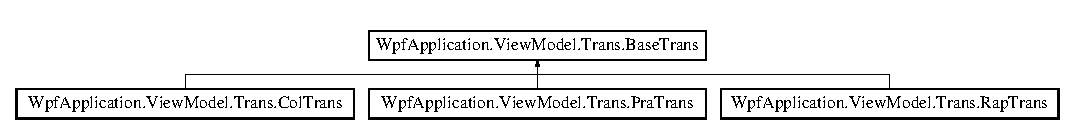
\includegraphics[height=1.372549cm]{class_wpf_application_1_1_view_model_1_1_trans_1_1_base_trans}
\end{center}
\end{figure}
\subsection*{Public Member Functions}
\begin{DoxyCompactItemize}
\item 
virtual string \hyperlink{class_wpf_application_1_1_view_model_1_1_trans_1_1_base_trans_a9660be8cb25ed5d666eab9ddd10600aa}{get\-Class} ()
\end{DoxyCompactItemize}


\subsection{Member Function Documentation}
\hypertarget{class_wpf_application_1_1_view_model_1_1_trans_1_1_base_trans_a9660be8cb25ed5d666eab9ddd10600aa}{\index{Wpf\-Application\-::\-View\-Model\-::\-Trans\-::\-Base\-Trans@{Wpf\-Application\-::\-View\-Model\-::\-Trans\-::\-Base\-Trans}!get\-Class@{get\-Class}}
\index{get\-Class@{get\-Class}!WpfApplication::ViewModel::Trans::BaseTrans@{Wpf\-Application\-::\-View\-Model\-::\-Trans\-::\-Base\-Trans}}
\subsubsection[{get\-Class}]{\setlength{\rightskip}{0pt plus 5cm}virtual string Wpf\-Application.\-View\-Model.\-Trans.\-Base\-Trans.\-get\-Class (
\begin{DoxyParamCaption}
{}
\end{DoxyParamCaption}
)\hspace{0.3cm}{\ttfamily [virtual]}}}\label{class_wpf_application_1_1_view_model_1_1_trans_1_1_base_trans_a9660be8cb25ed5d666eab9ddd10600aa}


Reimplemented in \hyperlink{class_wpf_application_1_1_view_model_1_1_trans_1_1_col_trans_aa3df7badaefa8f6adeb0de1147b649bc}{Wpf\-Application.\-View\-Model.\-Trans.\-Col\-Trans}, \hyperlink{class_wpf_application_1_1_view_model_1_1_trans_1_1_pra_trans_a69e0d0034568e424fc88995a8bbfc06c}{Wpf\-Application.\-View\-Model.\-Trans.\-Pra\-Trans}, and \hyperlink{class_wpf_application_1_1_view_model_1_1_trans_1_1_rap_trans_acbc5326d57143463f3d26fe66dab7a14}{Wpf\-Application.\-View\-Model.\-Trans.\-Rap\-Trans}.



The documentation for this class was generated from the following file\-:\begin{DoxyCompactItemize}
\item 
C\-:/\-Users/dju/\-Documents/\-Visual Studio 2012/\-Projects/\-P\-P\-E/\-P\-P\-E3/\-Wpf\-Application/\-View\-Model/\-Trans/\hyperlink{_base_trans_8cs}{Base\-Trans.\-cs}\end{DoxyCompactItemize}

\hypertarget{class_model_1_1_b_d_d___s_i_o7_entities}{\section{Model.\-B\-D\-D\-\_\-\-S\-I\-O7\-Entities Class Reference}
\label{class_model_1_1_b_d_d___s_i_o7_entities}\index{Model.\-B\-D\-D\-\_\-\-S\-I\-O7\-Entities@{Model.\-B\-D\-D\-\_\-\-S\-I\-O7\-Entities}}
}


Aucune documentation sur les métadonnées n'est disponible.  


Inheritance diagram for Model.\-B\-D\-D\-\_\-\-S\-I\-O7\-Entities\-:\begin{figure}[H]
\begin{center}
\leavevmode
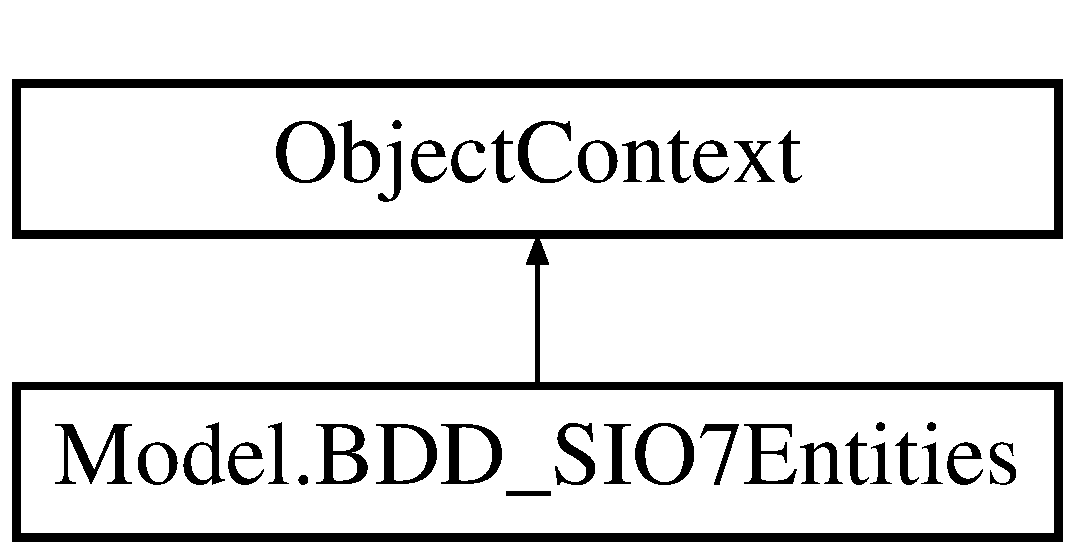
\includegraphics[height=2.000000cm]{class_model_1_1_b_d_d___s_i_o7_entities}
\end{center}
\end{figure}
\subsection*{Public Member Functions}
\begin{DoxyCompactItemize}
\item 
\hyperlink{class_model_1_1_b_d_d___s_i_o7_entities_a5dfa0a4c735cbeff99ed45c3f1f91a38}{B\-D\-D\-\_\-\-S\-I\-O7\-Entities} ()
\begin{DoxyCompactList}\small\item\em Initialise un nouvel objet \hyperlink{class_model_1_1_b_d_d___s_i_o7_entities}{B\-D\-D\-\_\-\-S\-I\-O7\-Entities} à l'aide de la chaîne de connexion trouvée dans la section '\hyperlink{class_model_1_1_b_d_d___s_i_o7_entities}{B\-D\-D\-\_\-\-S\-I\-O7\-Entities}' du fichier de configuration d'application. \end{DoxyCompactList}\item 
\hyperlink{class_model_1_1_b_d_d___s_i_o7_entities_aad5811b3abcd4987e89cb0e11e045382}{B\-D\-D\-\_\-\-S\-I\-O7\-Entities} (string connection\-String)
\begin{DoxyCompactList}\small\item\em Initialisez un nouvel objet \hyperlink{class_model_1_1_b_d_d___s_i_o7_entities}{B\-D\-D\-\_\-\-S\-I\-O7\-Entities}. \end{DoxyCompactList}\item 
\hyperlink{class_model_1_1_b_d_d___s_i_o7_entities_a6b57e3f7563e54b376cc5ed738db5db0}{B\-D\-D\-\_\-\-S\-I\-O7\-Entities} (Entity\-Connection connection)
\begin{DoxyCompactList}\small\item\em Initialisez un nouvel objet \hyperlink{class_model_1_1_b_d_d___s_i_o7_entities}{B\-D\-D\-\_\-\-S\-I\-O7\-Entities}. \end{DoxyCompactList}\item 
void \hyperlink{class_model_1_1_b_d_d___s_i_o7_entities_adf0f6d262f390e7bb0ccb29f060b77d4}{Add\-To\-A\-C\-T\-I\-V\-I\-T\-E\-\_\-\-C\-O\-M\-P\-L\-E\-M\-E\-N\-T\-A\-I\-R\-E} (\hyperlink{class_model_1_1_a_c_t_i_v_i_t_e___c_o_m_p_l_e_m_e_n_t_a_i_r_e}{A\-C\-T\-I\-V\-I\-T\-E\-\_\-\-C\-O\-M\-P\-L\-E\-M\-E\-N\-T\-A\-I\-R\-E} a\-C\-T\-I\-V\-I\-T\-E\-\_\-\-C\-O\-M\-P\-L\-E\-M\-E\-N\-T\-A\-I\-R\-E)
\begin{DoxyCompactList}\small\item\em Méthode déconseillée pour ajouter un nouvel objet à l'Entity\-Set \hyperlink{class_model_1_1_a_c_t_i_v_i_t_e___c_o_m_p_l_e_m_e_n_t_a_i_r_e}{A\-C\-T\-I\-V\-I\-T\-E\-\_\-\-C\-O\-M\-P\-L\-E\-M\-E\-N\-T\-A\-I\-R\-E}. Utilisez la méthode .Add de la propriété Object\-Set$<$T$>$ associée à la place. \end{DoxyCompactList}\item 
void \hyperlink{class_model_1_1_b_d_d___s_i_o7_entities_abf7d4c9ded0275437ebc16bc8ab3209b}{Add\-To\-C\-A\-L\-E\-N\-D\-R\-I\-E\-R} (\hyperlink{class_model_1_1_c_a_l_e_n_d_r_i_e_r}{C\-A\-L\-E\-N\-D\-R\-I\-E\-R} c\-A\-L\-E\-N\-D\-R\-I\-E\-R)
\begin{DoxyCompactList}\small\item\em Méthode déconseillée pour ajouter un nouvel objet à l'Entity\-Set \hyperlink{class_model_1_1_c_a_l_e_n_d_r_i_e_r}{C\-A\-L\-E\-N\-D\-R\-I\-E\-R}. Utilisez la méthode .Add de la propriété Object\-Set$<$T$>$ associée à la place. \end{DoxyCompactList}\item 
void \hyperlink{class_model_1_1_b_d_d___s_i_o7_entities_af367e2be722776185ac6d88229412936}{Add\-To\-C\-O\-L\-L\-A\-B\-O\-R\-A\-T\-E\-U\-R} (\hyperlink{class_model_1_1_c_o_l_l_a_b_o_r_a_t_e_u_r}{C\-O\-L\-L\-A\-B\-O\-R\-A\-T\-E\-U\-R} c\-O\-L\-L\-A\-B\-O\-R\-A\-T\-E\-U\-R)
\begin{DoxyCompactList}\small\item\em Méthode déconseillée pour ajouter un nouvel objet à l'Entity\-Set \hyperlink{class_model_1_1_c_o_l_l_a_b_o_r_a_t_e_u_r}{C\-O\-L\-L\-A\-B\-O\-R\-A\-T\-E\-U\-R}. Utilisez la méthode .Add de la propriété Object\-Set$<$T$>$ associée à la place. \end{DoxyCompactList}\item 
void \hyperlink{class_model_1_1_b_d_d___s_i_o7_entities_adb90d0998ce774a09ed413ec2302dda0}{Add\-To\-C\-O\-M\-M\-U\-N\-E} (\hyperlink{class_model_1_1_c_o_m_m_u_n_e}{C\-O\-M\-M\-U\-N\-E} c\-O\-M\-M\-U\-N\-E)
\begin{DoxyCompactList}\small\item\em Méthode déconseillée pour ajouter un nouvel objet à l'Entity\-Set \hyperlink{class_model_1_1_c_o_m_m_u_n_e}{C\-O\-M\-M\-U\-N\-E}. Utilisez la méthode .Add de la propriété Object\-Set$<$T$>$ associée à la place. \end{DoxyCompactList}\item 
void \hyperlink{class_model_1_1_b_d_d___s_i_o7_entities_acebebfec4025e3aa4d4b84cce87eb7f2}{Add\-To\-C\-O\-M\-P\-O\-S\-A\-N\-T} (\hyperlink{class_model_1_1_c_o_m_p_o_s_a_n_t}{C\-O\-M\-P\-O\-S\-A\-N\-T} c\-O\-M\-P\-O\-S\-A\-N\-T)
\begin{DoxyCompactList}\small\item\em Méthode déconseillée pour ajouter un nouvel objet à l'Entity\-Set \hyperlink{class_model_1_1_c_o_m_p_o_s_a_n_t}{C\-O\-M\-P\-O\-S\-A\-N\-T}. Utilisez la méthode .Add de la propriété Object\-Set$<$T$>$ associée à la place. \end{DoxyCompactList}\item 
void \hyperlink{class_model_1_1_b_d_d___s_i_o7_entities_aeeb273ac215656570d8b100487cc4062}{Add\-To\-D\-A\-T\-E} (\hyperlink{class_model_1_1_d_a_t_e}{D\-A\-T\-E} d\-A\-T\-E)
\begin{DoxyCompactList}\small\item\em Méthode déconseillée pour ajouter un nouvel objet à l'Entity\-Set \hyperlink{class_model_1_1_d_a_t_e}{D\-A\-T\-E}. Utilisez la méthode .Add de la propriété Object\-Set$<$T$>$ associée à la place. \end{DoxyCompactList}\item 
void \hyperlink{class_model_1_1_b_d_d___s_i_o7_entities_abaee891d220207d23a9ee04a1764b781}{Add\-To\-D\-E\-P\-A\-R\-T\-E\-M\-E\-N\-T} (\hyperlink{class_model_1_1_d_e_p_a_r_t_e_m_e_n_t}{D\-E\-P\-A\-R\-T\-E\-M\-E\-N\-T} d\-E\-P\-A\-R\-T\-E\-M\-E\-N\-T)
\begin{DoxyCompactList}\small\item\em Méthode déconseillée pour ajouter un nouvel objet à l'Entity\-Set \hyperlink{class_model_1_1_d_e_p_a_r_t_e_m_e_n_t}{D\-E\-P\-A\-R\-T\-E\-M\-E\-N\-T}. Utilisez la méthode .Add de la propriété Object\-Set$<$T$>$ associée à la place. \end{DoxyCompactList}\item 
void \hyperlink{class_model_1_1_b_d_d___s_i_o7_entities_a9ee07c8d5764c160ea9ddcf97936a69f}{Add\-To\-D\-I\-R\-E\-C\-T\-E\-U\-R\-\_\-\-R\-E\-G\-I\-O\-N\-A\-L} (\hyperlink{class_model_1_1_d_i_r_e_c_t_e_u_r___r_e_g_i_o_n_a_l}{D\-I\-R\-E\-C\-T\-E\-U\-R\-\_\-\-R\-E\-G\-I\-O\-N\-A\-L} d\-I\-R\-E\-C\-T\-E\-U\-R\-\_\-\-R\-E\-G\-I\-O\-N\-A\-L)
\begin{DoxyCompactList}\small\item\em Méthode déconseillée pour ajouter un nouvel objet à l'Entity\-Set \hyperlink{class_model_1_1_d_i_r_e_c_t_e_u_r___r_e_g_i_o_n_a_l}{D\-I\-R\-E\-C\-T\-E\-U\-R\-\_\-\-R\-E\-G\-I\-O\-N\-A\-L}. Utilisez la méthode .Add de la propriété Object\-Set$<$T$>$ associée à la place. \end{DoxyCompactList}\item 
void \hyperlink{class_model_1_1_b_d_d___s_i_o7_entities_a2a4456e3b6fe7f7ec716a9e8151513df}{Add\-To\-D\-O\-S\-A\-G\-E} (\hyperlink{class_model_1_1_d_o_s_a_g_e}{D\-O\-S\-A\-G\-E} d\-O\-S\-A\-G\-E)
\begin{DoxyCompactList}\small\item\em Méthode déconseillée pour ajouter un nouvel objet à l'Entity\-Set \hyperlink{class_model_1_1_d_o_s_a_g_e}{D\-O\-S\-A\-G\-E}. Utilisez la méthode .Add de la propriété Object\-Set$<$T$>$ associée à la place. \end{DoxyCompactList}\item 
void \hyperlink{class_model_1_1_b_d_d___s_i_o7_entities_a38c07ac029787f240fae431e141c2a65}{Add\-To\-E\-T\-R\-E\-\_\-\-R\-E\-S\-P\-O\-N\-S\-A\-B\-L\-E} (\hyperlink{class_model_1_1_e_t_r_e___r_e_s_p_o_n_s_a_b_l_e}{E\-T\-R\-E\-\_\-\-R\-E\-S\-P\-O\-N\-S\-A\-B\-L\-E} e\-T\-R\-E\-\_\-\-R\-E\-S\-P\-O\-N\-S\-A\-B\-L\-E)
\begin{DoxyCompactList}\small\item\em Méthode déconseillée pour ajouter un nouvel objet à l'Entity\-Set \hyperlink{class_model_1_1_e_t_r_e___r_e_s_p_o_n_s_a_b_l_e}{E\-T\-R\-E\-\_\-\-R\-E\-S\-P\-O\-N\-S\-A\-B\-L\-E}. Utilisez la méthode .Add de la propriété Object\-Set$<$T$>$ associée à la place. \end{DoxyCompactList}\item 
void \hyperlink{class_model_1_1_b_d_d___s_i_o7_entities_a68959da31b94dcaf686dd59b14d7f100}{Add\-To\-F\-A\-M\-I\-L\-L\-E} (\hyperlink{class_model_1_1_f_a_m_i_l_l_e}{F\-A\-M\-I\-L\-L\-E} f\-A\-M\-I\-L\-L\-E)
\begin{DoxyCompactList}\small\item\em Méthode déconseillée pour ajouter un nouvel objet à l'Entity\-Set \hyperlink{class_model_1_1_f_a_m_i_l_l_e}{F\-A\-M\-I\-L\-L\-E}. Utilisez la méthode .Add de la propriété Object\-Set$<$T$>$ associée à la place. \end{DoxyCompactList}\item 
void \hyperlink{class_model_1_1_b_d_d___s_i_o7_entities_a65054ac207f1923a158130403d84a28c}{Add\-To\-F\-I\-C\-H\-E\-\_\-\-F\-R\-A\-I\-S} (\hyperlink{class_model_1_1_f_i_c_h_e___f_r_a_i_s}{F\-I\-C\-H\-E\-\_\-\-F\-R\-A\-I\-S} f\-I\-C\-H\-E\-\_\-\-F\-R\-A\-I\-S)
\begin{DoxyCompactList}\small\item\em Méthode déconseillée pour ajouter un nouvel objet à l'Entity\-Set \hyperlink{class_model_1_1_f_i_c_h_e___f_r_a_i_s}{F\-I\-C\-H\-E\-\_\-\-F\-R\-A\-I\-S}. Utilisez la méthode .Add de la propriété Object\-Set$<$T$>$ associée à la place. \end{DoxyCompactList}\item 
void \hyperlink{class_model_1_1_b_d_d___s_i_o7_entities_a9e312e83af4743475e872fb79645bd73}{Add\-To\-G\-E\-R\-E} (\hyperlink{class_model_1_1_g_e_r_e}{G\-E\-R\-E} g\-E\-R\-E)
\begin{DoxyCompactList}\small\item\em Méthode déconseillée pour ajouter un nouvel objet à l'Entity\-Set \hyperlink{class_model_1_1_g_e_r_e}{G\-E\-R\-E}. Utilisez la méthode .Add de la propriété Object\-Set$<$T$>$ associée à la place. \end{DoxyCompactList}\item 
void \hyperlink{class_model_1_1_b_d_d___s_i_o7_entities_a612c8d919e09d81c47301d83e153e684}{Add\-To\-M\-E\-D\-I\-C\-A\-M\-E\-N\-T} (\hyperlink{class_model_1_1_m_e_d_i_c_a_m_e_n_t}{M\-E\-D\-I\-C\-A\-M\-E\-N\-T} m\-E\-D\-I\-C\-A\-M\-E\-N\-T)
\begin{DoxyCompactList}\small\item\em Méthode déconseillée pour ajouter un nouvel objet à l'Entity\-Set \hyperlink{class_model_1_1_m_e_d_i_c_a_m_e_n_t}{M\-E\-D\-I\-C\-A\-M\-E\-N\-T}. Utilisez la méthode .Add de la propriété Object\-Set$<$T$>$ associée à la place. \end{DoxyCompactList}\item 
void \hyperlink{class_model_1_1_b_d_d___s_i_o7_entities_a094dc07ad708a675e828b33fc869fda5}{Add\-To\-M\-O\-T\-I\-F} (\hyperlink{class_model_1_1_m_o_t_i_f}{M\-O\-T\-I\-F} m\-O\-T\-I\-F)
\begin{DoxyCompactList}\small\item\em Méthode déconseillée pour ajouter un nouvel objet à l'Entity\-Set \hyperlink{class_model_1_1_m_o_t_i_f}{M\-O\-T\-I\-F}. Utilisez la méthode .Add de la propriété Object\-Set$<$T$>$ associée à la place. \end{DoxyCompactList}\item 
void \hyperlink{class_model_1_1_b_d_d___s_i_o7_entities_a7e4687bf54919ebb25e95f2b0c1ee5cd}{Add\-To\-P\-R\-A\-T\-I\-C\-I\-E\-N} (\hyperlink{class_model_1_1_p_r_a_t_i_c_i_e_n}{P\-R\-A\-T\-I\-C\-I\-E\-N} p\-R\-A\-T\-I\-C\-I\-E\-N)
\begin{DoxyCompactList}\small\item\em Méthode déconseillée pour ajouter un nouvel objet à l'Entity\-Set \hyperlink{class_model_1_1_p_r_a_t_i_c_i_e_n}{P\-R\-A\-T\-I\-C\-I\-E\-N}. Utilisez la méthode .Add de la propriété Object\-Set$<$T$>$ associée à la place. \end{DoxyCompactList}\item 
void \hyperlink{class_model_1_1_b_d_d___s_i_o7_entities_accc4001cadd40aa0e911ee9e01b534bf}{Add\-To\-P\-R\-E\-S\-C\-R\-I\-R\-E} (\hyperlink{class_model_1_1_p_r_e_s_c_r_i_r_e}{P\-R\-E\-S\-C\-R\-I\-R\-E} p\-R\-E\-S\-C\-R\-I\-R\-E)
\begin{DoxyCompactList}\small\item\em Méthode déconseillée pour ajouter un nouvel objet à l'Entity\-Set \hyperlink{class_model_1_1_p_r_e_s_c_r_i_r_e}{P\-R\-E\-S\-C\-R\-I\-R\-E}. Utilisez la méthode .Add de la propriété Object\-Set$<$T$>$ associée à la place. \end{DoxyCompactList}\item 
void \hyperlink{class_model_1_1_b_d_d___s_i_o7_entities_a938f7a337f50c5fe23df54fe9b70aecb}{Add\-To\-P\-R\-E\-S\-E\-N\-T\-A\-T\-I\-O\-N} (\hyperlink{class_model_1_1_p_r_e_s_e_n_t_a_t_i_o_n}{P\-R\-E\-S\-E\-N\-T\-A\-T\-I\-O\-N} p\-R\-E\-S\-E\-N\-T\-A\-T\-I\-O\-N)
\begin{DoxyCompactList}\small\item\em Méthode déconseillée pour ajouter un nouvel objet à l'Entity\-Set \hyperlink{class_model_1_1_p_r_e_s_e_n_t_a_t_i_o_n}{P\-R\-E\-S\-E\-N\-T\-A\-T\-I\-O\-N}. Utilisez la méthode .Add de la propriété Object\-Set$<$T$>$ associée à la place. \end{DoxyCompactList}\item 
void \hyperlink{class_model_1_1_b_d_d___s_i_o7_entities_a8fd3f511e9e94cebbf9c19f3ada21bc8}{Add\-To\-R\-A\-P\-P\-O\-R\-T\-\_\-\-D\-E\-\_\-\-V\-I\-S\-I\-T\-E} (\hyperlink{class_model_1_1_r_a_p_p_o_r_t___d_e___v_i_s_i_t_e}{R\-A\-P\-P\-O\-R\-T\-\_\-\-D\-E\-\_\-\-V\-I\-S\-I\-T\-E} r\-A\-P\-P\-O\-R\-T\-\_\-\-D\-E\-\_\-\-V\-I\-S\-I\-T\-E)
\begin{DoxyCompactList}\small\item\em Méthode déconseillée pour ajouter un nouvel objet à l'Entity\-Set \hyperlink{class_model_1_1_r_a_p_p_o_r_t___d_e___v_i_s_i_t_e}{R\-A\-P\-P\-O\-R\-T\-\_\-\-D\-E\-\_\-\-V\-I\-S\-I\-T\-E}. Utilisez la méthode .Add de la propriété Object\-Set$<$T$>$ associée à la place. \end{DoxyCompactList}\item 
void \hyperlink{class_model_1_1_b_d_d___s_i_o7_entities_a822bd2f146c15c04bbaf6e7ad30fc202}{Add\-To\-R\-E\-G\-I\-O\-N} (\hyperlink{class_model_1_1_r_e_g_i_o_n}{R\-E\-G\-I\-O\-N} r\-E\-G\-I\-O\-N)
\begin{DoxyCompactList}\small\item\em Méthode déconseillée pour ajouter un nouvel objet à l'Entity\-Set \hyperlink{class_model_1_1_r_e_g_i_o_n}{R\-E\-G\-I\-O\-N}. Utilisez la méthode .Add de la propriété Object\-Set$<$T$>$ associée à la place. \end{DoxyCompactList}\item 
void \hyperlink{class_model_1_1_b_d_d___s_i_o7_entities_a89ca2a21b6b7fbb4a1c42864dd8ed904}{Add\-To\-R\-E\-M\-P\-L\-A\-C\-E} (\hyperlink{class_model_1_1_r_e_m_p_l_a_c_e}{R\-E\-M\-P\-L\-A\-C\-E} r\-E\-M\-P\-L\-A\-C\-E)
\begin{DoxyCompactList}\small\item\em Méthode déconseillée pour ajouter un nouvel objet à l'Entity\-Set \hyperlink{class_model_1_1_r_e_m_p_l_a_c_e}{R\-E\-M\-P\-L\-A\-C\-E}. Utilisez la méthode .Add de la propriété Object\-Set$<$T$>$ associée à la place. \end{DoxyCompactList}\item 
void \hyperlink{class_model_1_1_b_d_d___s_i_o7_entities_a5ae40a9b13130c06ad72686eccf0c651}{Add\-To\-R\-E\-S\-P\-O\-N\-S\-A\-B\-L\-E\-\_\-\-D\-E\-\_\-\-S\-E\-C\-T\-E\-U\-R} (\hyperlink{class_model_1_1_r_e_s_p_o_n_s_a_b_l_e___d_e___s_e_c_t_e_u_r}{R\-E\-S\-P\-O\-N\-S\-A\-B\-L\-E\-\_\-\-D\-E\-\_\-\-S\-E\-C\-T\-E\-U\-R} r\-E\-S\-P\-O\-N\-S\-A\-B\-L\-E\-\_\-\-D\-E\-\_\-\-S\-E\-C\-T\-E\-U\-R)
\begin{DoxyCompactList}\small\item\em Méthode déconseillée pour ajouter un nouvel objet à l'Entity\-Set \hyperlink{class_model_1_1_r_e_s_p_o_n_s_a_b_l_e___d_e___s_e_c_t_e_u_r}{R\-E\-S\-P\-O\-N\-S\-A\-B\-L\-E\-\_\-\-D\-E\-\_\-\-S\-E\-C\-T\-E\-U\-R}. Utilisez la méthode .Add de la propriété Object\-Set$<$T$>$ associée à la place. \end{DoxyCompactList}\item 
void \hyperlink{class_model_1_1_b_d_d___s_i_o7_entities_a318cd3b2de71c646c8bed25e9d6eb058}{Add\-To\-S\-E\-C\-T\-E\-U\-R} (\hyperlink{class_model_1_1_s_e_c_t_e_u_r}{S\-E\-C\-T\-E\-U\-R} s\-E\-C\-T\-E\-U\-R)
\begin{DoxyCompactList}\small\item\em Méthode déconseillée pour ajouter un nouvel objet à l'Entity\-Set \hyperlink{class_model_1_1_s_e_c_t_e_u_r}{S\-E\-C\-T\-E\-U\-R}. Utilisez la méthode .Add de la propriété Object\-Set$<$T$>$ associée à la place. \end{DoxyCompactList}\item 
void \hyperlink{class_model_1_1_b_d_d___s_i_o7_entities_a64639974a9e6ce0b8100dd1066da38de}{Add\-To\-S\-P\-E\-C\-I\-A\-L\-I\-T\-E} (\hyperlink{class_model_1_1_s_p_e_c_i_a_l_i_t_e}{S\-P\-E\-C\-I\-A\-L\-I\-T\-E} s\-P\-E\-C\-I\-A\-L\-I\-T\-E)
\begin{DoxyCompactList}\small\item\em Méthode déconseillée pour ajouter un nouvel objet à l'Entity\-Set \hyperlink{class_model_1_1_s_p_e_c_i_a_l_i_t_e}{S\-P\-E\-C\-I\-A\-L\-I\-T\-E}. Utilisez la méthode .Add de la propriété Object\-Set$<$T$>$ associée à la place. \end{DoxyCompactList}\item 
void \hyperlink{class_model_1_1_b_d_d___s_i_o7_entities_a729996d8d2afd99e05fcaaed4c232af6}{Add\-Tosysdiagrams} (\hyperlink{class_model_1_1sysdiagrams}{sysdiagrams} \hyperlink{class_model_1_1sysdiagrams}{sysdiagrams})
\begin{DoxyCompactList}\small\item\em Méthode déconseillée pour ajouter un nouvel objet à l'Entity\-Set sysdiagrams. Utilisez la méthode .Add de la propriété Object\-Set$<$T$>$ associée à la place. \end{DoxyCompactList}\item 
void \hyperlink{class_model_1_1_b_d_d___s_i_o7_entities_a432ca0b9d17f17d569c6db05bb44239d}{Add\-To\-T\-Y\-P\-E\-\_\-\-F\-R\-A\-I\-S} (\hyperlink{class_model_1_1_t_y_p_e___f_r_a_i_s}{T\-Y\-P\-E\-\_\-\-F\-R\-A\-I\-S} t\-Y\-P\-E\-\_\-\-F\-R\-A\-I\-S)
\begin{DoxyCompactList}\small\item\em Méthode déconseillée pour ajouter un nouvel objet à l'Entity\-Set \hyperlink{class_model_1_1_t_y_p_e___f_r_a_i_s}{T\-Y\-P\-E\-\_\-\-F\-R\-A\-I\-S}. Utilisez la méthode .Add de la propriété Object\-Set$<$T$>$ associée à la place. \end{DoxyCompactList}\item 
void \hyperlink{class_model_1_1_b_d_d___s_i_o7_entities_a4e51f7a72211f52bb10b28f6aba0dbe1}{Add\-To\-T\-Y\-P\-E\-\_\-\-I\-N\-D\-I\-V\-I\-D\-U} (\hyperlink{class_model_1_1_t_y_p_e___i_n_d_i_v_i_d_u}{T\-Y\-P\-E\-\_\-\-I\-N\-D\-I\-V\-I\-D\-U} t\-Y\-P\-E\-\_\-\-I\-N\-D\-I\-V\-I\-D\-U)
\begin{DoxyCompactList}\small\item\em Méthode déconseillée pour ajouter un nouvel objet à l'Entity\-Set \hyperlink{class_model_1_1_t_y_p_e___i_n_d_i_v_i_d_u}{T\-Y\-P\-E\-\_\-\-I\-N\-D\-I\-V\-I\-D\-U}. Utilisez la méthode .Add de la propriété Object\-Set$<$T$>$ associée à la place. \end{DoxyCompactList}\item 
void \hyperlink{class_model_1_1_b_d_d___s_i_o7_entities_a7f21aafcf6df9a79fcbc6036fda23f8e}{Add\-To\-T\-Y\-P\-E\-\_\-\-P\-R\-A\-T\-I\-C\-I\-E\-N} (\hyperlink{class_model_1_1_t_y_p_e___p_r_a_t_i_c_i_e_n}{T\-Y\-P\-E\-\_\-\-P\-R\-A\-T\-I\-C\-I\-E\-N} t\-Y\-P\-E\-\_\-\-P\-R\-A\-T\-I\-C\-I\-E\-N)
\begin{DoxyCompactList}\small\item\em Méthode déconseillée pour ajouter un nouvel objet à l'Entity\-Set \hyperlink{class_model_1_1_t_y_p_e___p_r_a_t_i_c_i_e_n}{T\-Y\-P\-E\-\_\-\-P\-R\-A\-T\-I\-C\-I\-E\-N}. Utilisez la méthode .Add de la propriété Object\-Set$<$T$>$ associée à la place. \end{DoxyCompactList}\item 
void \hyperlink{class_model_1_1_b_d_d___s_i_o7_entities_a62c2e84fc50405caf6ad75ed7e4cc318}{Add\-To\-V\-I\-S\-I\-T\-E\-U\-R} (\hyperlink{class_model_1_1_v_i_s_i_t_e_u_r}{V\-I\-S\-I\-T\-E\-U\-R} v\-I\-S\-I\-T\-E\-U\-R)
\begin{DoxyCompactList}\small\item\em Méthode déconseillée pour ajouter un nouvel objet à l'Entity\-Set \hyperlink{class_model_1_1_v_i_s_i_t_e_u_r}{V\-I\-S\-I\-T\-E\-U\-R}. Utilisez la méthode .Add de la propriété Object\-Set$<$T$>$ associée à la place. \end{DoxyCompactList}\item 
void \hyperlink{class_model_1_1_b_d_d___s_i_o7_entities_aca1c2afc639447dc937518b9f5f7046a}{Add\-To\-O\-F\-F\-R\-E1\-Jeu} (\hyperlink{class_model_1_1_o_f_f_r_e1}{O\-F\-F\-R\-E1} o\-F\-F\-R\-E1)
\begin{DoxyCompactList}\small\item\em Méthode déconseillée pour ajouter un nouvel objet à l'Entity\-Set O\-F\-F\-R\-E1\-Jeu. Utilisez la méthode .Add de la propriété Object\-Set$<$T$>$ associée à la place. \end{DoxyCompactList}\item 
void \hyperlink{class_model_1_1_b_d_d___s_i_o7_entities_a77379f47a61f5e58dd59851d30ad6f4f}{Add\-To\-P\-R\-E\-S\-E\-N\-T\-E} (\hyperlink{class_model_1_1_p_r_e_s_e_n_t_e}{P\-R\-E\-S\-E\-N\-T\-E} p\-R\-E\-S\-E\-N\-T\-E)
\begin{DoxyCompactList}\small\item\em Méthode déconseillée pour ajouter un nouvel objet à l'Entity\-Set \hyperlink{class_model_1_1_p_r_e_s_e_n_t_e}{P\-R\-E\-S\-E\-N\-T\-E}. Utilisez la méthode .Add de la propriété Object\-Set$<$T$>$ associée à la place. \end{DoxyCompactList}\item 
void \hyperlink{class_model_1_1_b_d_d___s_i_o7_entities_a9510bff763ce90ed7ab7aaeca09b31cc}{Add\-To\-A\-V\-O\-I\-R1\-Jeu} (\hyperlink{class_model_1_1_a_v_o_i_r1}{A\-V\-O\-I\-R1} a\-V\-O\-I\-R1)
\begin{DoxyCompactList}\small\item\em Méthode déconseillée pour ajouter un nouvel objet à l'Entity\-Set A\-V\-O\-I\-R1\-Jeu. Utilisez la méthode .Add de la propriété Object\-Set$<$T$>$ associée à la place. \end{DoxyCompactList}\end{DoxyCompactItemize}
\subsection*{Properties}
\begin{DoxyCompactItemize}
\item 
Object\-Set\\*
$<$ \hyperlink{class_model_1_1_a_c_t_i_v_i_t_e___c_o_m_p_l_e_m_e_n_t_a_i_r_e}{A\-C\-T\-I\-V\-I\-T\-E\-\_\-\-C\-O\-M\-P\-L\-E\-M\-E\-N\-T\-A\-I\-R\-E} $>$ \hyperlink{class_model_1_1_b_d_d___s_i_o7_entities_a709b82c58993d3301d8fb850ff569654}{A\-C\-T\-I\-V\-I\-T\-E\-\_\-\-C\-O\-M\-P\-L\-E\-M\-E\-N\-T\-A\-I\-R\-E}\hspace{0.3cm}{\ttfamily  \mbox{[}get\mbox{]}}
\begin{DoxyCompactList}\small\item\em Aucune documentation sur les métadonnées n'est disponible. \end{DoxyCompactList}\item 
Object\-Set$<$ \hyperlink{class_model_1_1_c_a_l_e_n_d_r_i_e_r}{C\-A\-L\-E\-N\-D\-R\-I\-E\-R} $>$ \hyperlink{class_model_1_1_b_d_d___s_i_o7_entities_af6cdc5ecd7668ffe0331bcf663733351}{C\-A\-L\-E\-N\-D\-R\-I\-E\-R}\hspace{0.3cm}{\ttfamily  \mbox{[}get\mbox{]}}
\begin{DoxyCompactList}\small\item\em Aucune documentation sur les métadonnées n'est disponible. \end{DoxyCompactList}\item 
Object\-Set$<$ \hyperlink{class_model_1_1_c_o_l_l_a_b_o_r_a_t_e_u_r}{C\-O\-L\-L\-A\-B\-O\-R\-A\-T\-E\-U\-R} $>$ \hyperlink{class_model_1_1_b_d_d___s_i_o7_entities_a40ce35269025503e79db707928e426cb}{C\-O\-L\-L\-A\-B\-O\-R\-A\-T\-E\-U\-R}\hspace{0.3cm}{\ttfamily  \mbox{[}get\mbox{]}}
\begin{DoxyCompactList}\small\item\em Aucune documentation sur les métadonnées n'est disponible. \end{DoxyCompactList}\item 
Object\-Set$<$ \hyperlink{class_model_1_1_c_o_m_m_u_n_e}{C\-O\-M\-M\-U\-N\-E} $>$ \hyperlink{class_model_1_1_b_d_d___s_i_o7_entities_abae02e6727c53ad93c03d782dc106fb4}{C\-O\-M\-M\-U\-N\-E}\hspace{0.3cm}{\ttfamily  \mbox{[}get\mbox{]}}
\begin{DoxyCompactList}\small\item\em Aucune documentation sur les métadonnées n'est disponible. \end{DoxyCompactList}\item 
Object\-Set$<$ \hyperlink{class_model_1_1_c_o_m_p_o_s_a_n_t}{C\-O\-M\-P\-O\-S\-A\-N\-T} $>$ \hyperlink{class_model_1_1_b_d_d___s_i_o7_entities_a5ef1a59c0bb85f597274b5c08a6cf511}{C\-O\-M\-P\-O\-S\-A\-N\-T}\hspace{0.3cm}{\ttfamily  \mbox{[}get\mbox{]}}
\begin{DoxyCompactList}\small\item\em Aucune documentation sur les métadonnées n'est disponible. \end{DoxyCompactList}\item 
Object\-Set$<$ \hyperlink{class_model_1_1_d_a_t_e}{D\-A\-T\-E} $>$ \hyperlink{class_model_1_1_b_d_d___s_i_o7_entities_ab13a7822afc52c06d029c60e43d291cf}{D\-A\-T\-E}\hspace{0.3cm}{\ttfamily  \mbox{[}get\mbox{]}}
\begin{DoxyCompactList}\small\item\em Aucune documentation sur les métadonnées n'est disponible. \end{DoxyCompactList}\item 
Object\-Set$<$ \hyperlink{class_model_1_1_d_e_p_a_r_t_e_m_e_n_t}{D\-E\-P\-A\-R\-T\-E\-M\-E\-N\-T} $>$ \hyperlink{class_model_1_1_b_d_d___s_i_o7_entities_a4bade7b78d4a579cdd6690d69ba0c131}{D\-E\-P\-A\-R\-T\-E\-M\-E\-N\-T}\hspace{0.3cm}{\ttfamily  \mbox{[}get\mbox{]}}
\begin{DoxyCompactList}\small\item\em Aucune documentation sur les métadonnées n'est disponible. \end{DoxyCompactList}\item 
Object\-Set$<$ \hyperlink{class_model_1_1_d_i_r_e_c_t_e_u_r___r_e_g_i_o_n_a_l}{D\-I\-R\-E\-C\-T\-E\-U\-R\-\_\-\-R\-E\-G\-I\-O\-N\-A\-L} $>$ \hyperlink{class_model_1_1_b_d_d___s_i_o7_entities_a57e9f9cd0a56bd3698866941b6e2dbb3}{D\-I\-R\-E\-C\-T\-E\-U\-R\-\_\-\-R\-E\-G\-I\-O\-N\-A\-L}\hspace{0.3cm}{\ttfamily  \mbox{[}get\mbox{]}}
\begin{DoxyCompactList}\small\item\em Aucune documentation sur les métadonnées n'est disponible. \end{DoxyCompactList}\item 
Object\-Set$<$ \hyperlink{class_model_1_1_d_o_s_a_g_e}{D\-O\-S\-A\-G\-E} $>$ \hyperlink{class_model_1_1_b_d_d___s_i_o7_entities_ac901579b6afd772748e68adb8bd2e0f7}{D\-O\-S\-A\-G\-E}\hspace{0.3cm}{\ttfamily  \mbox{[}get\mbox{]}}
\begin{DoxyCompactList}\small\item\em Aucune documentation sur les métadonnées n'est disponible. \end{DoxyCompactList}\item 
Object\-Set$<$ \hyperlink{class_model_1_1_e_t_r_e___r_e_s_p_o_n_s_a_b_l_e}{E\-T\-R\-E\-\_\-\-R\-E\-S\-P\-O\-N\-S\-A\-B\-L\-E} $>$ \hyperlink{class_model_1_1_b_d_d___s_i_o7_entities_a1dbcb102b5850c6301a5572fc07a6197}{E\-T\-R\-E\-\_\-\-R\-E\-S\-P\-O\-N\-S\-A\-B\-L\-E}\hspace{0.3cm}{\ttfamily  \mbox{[}get\mbox{]}}
\begin{DoxyCompactList}\small\item\em Aucune documentation sur les métadonnées n'est disponible. \end{DoxyCompactList}\item 
Object\-Set$<$ \hyperlink{class_model_1_1_f_a_m_i_l_l_e}{F\-A\-M\-I\-L\-L\-E} $>$ \hyperlink{class_model_1_1_b_d_d___s_i_o7_entities_a8fa0833a2b61c9d1f6d20a5c207f0f08}{F\-A\-M\-I\-L\-L\-E}\hspace{0.3cm}{\ttfamily  \mbox{[}get\mbox{]}}
\begin{DoxyCompactList}\small\item\em Aucune documentation sur les métadonnées n'est disponible. \end{DoxyCompactList}\item 
Object\-Set$<$ \hyperlink{class_model_1_1_f_i_c_h_e___f_r_a_i_s}{F\-I\-C\-H\-E\-\_\-\-F\-R\-A\-I\-S} $>$ \hyperlink{class_model_1_1_b_d_d___s_i_o7_entities_a8dc9fa4a25f4ad033b363e8d1edb07d0}{F\-I\-C\-H\-E\-\_\-\-F\-R\-A\-I\-S}\hspace{0.3cm}{\ttfamily  \mbox{[}get\mbox{]}}
\begin{DoxyCompactList}\small\item\em Aucune documentation sur les métadonnées n'est disponible. \end{DoxyCompactList}\item 
Object\-Set$<$ \hyperlink{class_model_1_1_g_e_r_e}{G\-E\-R\-E} $>$ \hyperlink{class_model_1_1_b_d_d___s_i_o7_entities_af2d24722ba6d84b64960611c55b23327}{G\-E\-R\-E}\hspace{0.3cm}{\ttfamily  \mbox{[}get\mbox{]}}
\begin{DoxyCompactList}\small\item\em Aucune documentation sur les métadonnées n'est disponible. \end{DoxyCompactList}\item 
Object\-Set$<$ \hyperlink{class_model_1_1_m_e_d_i_c_a_m_e_n_t}{M\-E\-D\-I\-C\-A\-M\-E\-N\-T} $>$ \hyperlink{class_model_1_1_b_d_d___s_i_o7_entities_a21a0b47c75a9adef3ef5aee8ecedbd37}{M\-E\-D\-I\-C\-A\-M\-E\-N\-T}\hspace{0.3cm}{\ttfamily  \mbox{[}get\mbox{]}}
\begin{DoxyCompactList}\small\item\em Aucune documentation sur les métadonnées n'est disponible. \end{DoxyCompactList}\item 
Object\-Set$<$ \hyperlink{class_model_1_1_m_o_t_i_f}{M\-O\-T\-I\-F} $>$ \hyperlink{class_model_1_1_b_d_d___s_i_o7_entities_a9bf34ee977b7f671e9996967d1ff2328}{M\-O\-T\-I\-F}\hspace{0.3cm}{\ttfamily  \mbox{[}get\mbox{]}}
\begin{DoxyCompactList}\small\item\em Aucune documentation sur les métadonnées n'est disponible. \end{DoxyCompactList}\item 
Object\-Set$<$ \hyperlink{class_model_1_1_p_r_a_t_i_c_i_e_n}{P\-R\-A\-T\-I\-C\-I\-E\-N} $>$ \hyperlink{class_model_1_1_b_d_d___s_i_o7_entities_aa7f5305d592739cf4e3805fcdb0277ae}{P\-R\-A\-T\-I\-C\-I\-E\-N}\hspace{0.3cm}{\ttfamily  \mbox{[}get\mbox{]}}
\begin{DoxyCompactList}\small\item\em Aucune documentation sur les métadonnées n'est disponible. \end{DoxyCompactList}\item 
Object\-Set$<$ \hyperlink{class_model_1_1_p_r_e_s_c_r_i_r_e}{P\-R\-E\-S\-C\-R\-I\-R\-E} $>$ \hyperlink{class_model_1_1_b_d_d___s_i_o7_entities_a2f477606bede8c5cc3edbdddeb81ada8}{P\-R\-E\-S\-C\-R\-I\-R\-E}\hspace{0.3cm}{\ttfamily  \mbox{[}get\mbox{]}}
\begin{DoxyCompactList}\small\item\em Aucune documentation sur les métadonnées n'est disponible. \end{DoxyCompactList}\item 
Object\-Set$<$ \hyperlink{class_model_1_1_p_r_e_s_e_n_t_a_t_i_o_n}{P\-R\-E\-S\-E\-N\-T\-A\-T\-I\-O\-N} $>$ \hyperlink{class_model_1_1_b_d_d___s_i_o7_entities_a8e445ba6656fc5fe0d0b5fa5a391689e}{P\-R\-E\-S\-E\-N\-T\-A\-T\-I\-O\-N}\hspace{0.3cm}{\ttfamily  \mbox{[}get\mbox{]}}
\begin{DoxyCompactList}\small\item\em Aucune documentation sur les métadonnées n'est disponible. \end{DoxyCompactList}\item 
Object\-Set$<$ \hyperlink{class_model_1_1_r_a_p_p_o_r_t___d_e___v_i_s_i_t_e}{R\-A\-P\-P\-O\-R\-T\-\_\-\-D\-E\-\_\-\-V\-I\-S\-I\-T\-E} $>$ \hyperlink{class_model_1_1_b_d_d___s_i_o7_entities_a965f341d58028327c607a34ec17fcafc}{R\-A\-P\-P\-O\-R\-T\-\_\-\-D\-E\-\_\-\-V\-I\-S\-I\-T\-E}\hspace{0.3cm}{\ttfamily  \mbox{[}get\mbox{]}}
\begin{DoxyCompactList}\small\item\em Aucune documentation sur les métadonnées n'est disponible. \end{DoxyCompactList}\item 
Object\-Set$<$ \hyperlink{class_model_1_1_r_e_g_i_o_n}{R\-E\-G\-I\-O\-N} $>$ \hyperlink{class_model_1_1_b_d_d___s_i_o7_entities_abd0de3daf7a53c5a9b8d90c24bb67971}{R\-E\-G\-I\-O\-N}\hspace{0.3cm}{\ttfamily  \mbox{[}get\mbox{]}}
\begin{DoxyCompactList}\small\item\em Aucune documentation sur les métadonnées n'est disponible. \end{DoxyCompactList}\item 
Object\-Set$<$ \hyperlink{class_model_1_1_r_e_m_p_l_a_c_e}{R\-E\-M\-P\-L\-A\-C\-E} $>$ \hyperlink{class_model_1_1_b_d_d___s_i_o7_entities_a7403c47fc7f420ea1ad4f103a12b96c5}{R\-E\-M\-P\-L\-A\-C\-E}\hspace{0.3cm}{\ttfamily  \mbox{[}get\mbox{]}}
\begin{DoxyCompactList}\small\item\em Aucune documentation sur les métadonnées n'est disponible. \end{DoxyCompactList}\item 
Object\-Set$<$ \hyperlink{class_model_1_1_r_e_s_p_o_n_s_a_b_l_e___d_e___s_e_c_t_e_u_r}{R\-E\-S\-P\-O\-N\-S\-A\-B\-L\-E\-\_\-\-D\-E\-\_\-\-S\-E\-C\-T\-E\-U\-R} $>$ \hyperlink{class_model_1_1_b_d_d___s_i_o7_entities_a6176c375621ed6fa48307b4c0c12c030}{R\-E\-S\-P\-O\-N\-S\-A\-B\-L\-E\-\_\-\-D\-E\-\_\-\-S\-E\-C\-T\-E\-U\-R}\hspace{0.3cm}{\ttfamily  \mbox{[}get\mbox{]}}
\begin{DoxyCompactList}\small\item\em Aucune documentation sur les métadonnées n'est disponible. \end{DoxyCompactList}\item 
Object\-Set$<$ \hyperlink{class_model_1_1_s_e_c_t_e_u_r}{S\-E\-C\-T\-E\-U\-R} $>$ \hyperlink{class_model_1_1_b_d_d___s_i_o7_entities_a6c7e5e2098c03456f950dd088b6507ef}{S\-E\-C\-T\-E\-U\-R}\hspace{0.3cm}{\ttfamily  \mbox{[}get\mbox{]}}
\begin{DoxyCompactList}\small\item\em Aucune documentation sur les métadonnées n'est disponible. \end{DoxyCompactList}\item 
Object\-Set$<$ \hyperlink{class_model_1_1_s_p_e_c_i_a_l_i_t_e}{S\-P\-E\-C\-I\-A\-L\-I\-T\-E} $>$ \hyperlink{class_model_1_1_b_d_d___s_i_o7_entities_ac2e52a3850fb20c481adac53dd529ab0}{S\-P\-E\-C\-I\-A\-L\-I\-T\-E}\hspace{0.3cm}{\ttfamily  \mbox{[}get\mbox{]}}
\begin{DoxyCompactList}\small\item\em Aucune documentation sur les métadonnées n'est disponible. \end{DoxyCompactList}\item 
Object\-Set$<$ \hyperlink{class_model_1_1sysdiagrams}{sysdiagrams} $>$ \hyperlink{class_model_1_1_b_d_d___s_i_o7_entities_a58f4c74a27a387297972be29496fd65b}{sysdiagrams}\hspace{0.3cm}{\ttfamily  \mbox{[}get\mbox{]}}
\begin{DoxyCompactList}\small\item\em Aucune documentation sur les métadonnées n'est disponible. \end{DoxyCompactList}\item 
Object\-Set$<$ \hyperlink{class_model_1_1_t_y_p_e___f_r_a_i_s}{T\-Y\-P\-E\-\_\-\-F\-R\-A\-I\-S} $>$ \hyperlink{class_model_1_1_b_d_d___s_i_o7_entities_a9a8272432096c86002858504785d663d}{T\-Y\-P\-E\-\_\-\-F\-R\-A\-I\-S}\hspace{0.3cm}{\ttfamily  \mbox{[}get\mbox{]}}
\begin{DoxyCompactList}\small\item\em Aucune documentation sur les métadonnées n'est disponible. \end{DoxyCompactList}\item 
Object\-Set$<$ \hyperlink{class_model_1_1_t_y_p_e___i_n_d_i_v_i_d_u}{T\-Y\-P\-E\-\_\-\-I\-N\-D\-I\-V\-I\-D\-U} $>$ \hyperlink{class_model_1_1_b_d_d___s_i_o7_entities_a1b24dfc017d342ad01ac90045173c72c}{T\-Y\-P\-E\-\_\-\-I\-N\-D\-I\-V\-I\-D\-U}\hspace{0.3cm}{\ttfamily  \mbox{[}get\mbox{]}}
\begin{DoxyCompactList}\small\item\em Aucune documentation sur les métadonnées n'est disponible. \end{DoxyCompactList}\item 
Object\-Set$<$ \hyperlink{class_model_1_1_t_y_p_e___p_r_a_t_i_c_i_e_n}{T\-Y\-P\-E\-\_\-\-P\-R\-A\-T\-I\-C\-I\-E\-N} $>$ \hyperlink{class_model_1_1_b_d_d___s_i_o7_entities_a01d5e4265274c8d01bf75377b41cb595}{T\-Y\-P\-E\-\_\-\-P\-R\-A\-T\-I\-C\-I\-E\-N}\hspace{0.3cm}{\ttfamily  \mbox{[}get\mbox{]}}
\begin{DoxyCompactList}\small\item\em Aucune documentation sur les métadonnées n'est disponible. \end{DoxyCompactList}\item 
Object\-Set$<$ \hyperlink{class_model_1_1_v_i_s_i_t_e_u_r}{V\-I\-S\-I\-T\-E\-U\-R} $>$ \hyperlink{class_model_1_1_b_d_d___s_i_o7_entities_a6bea95538ec6b785b1b5bf6e8d9f5efd}{V\-I\-S\-I\-T\-E\-U\-R}\hspace{0.3cm}{\ttfamily  \mbox{[}get\mbox{]}}
\begin{DoxyCompactList}\small\item\em Aucune documentation sur les métadonnées n'est disponible. \end{DoxyCompactList}\item 
Object\-Set$<$ \hyperlink{class_model_1_1_o_f_f_r_e1}{O\-F\-F\-R\-E1} $>$ \hyperlink{class_model_1_1_b_d_d___s_i_o7_entities_a3430fda13ad472d300b07c477b43b6b6}{O\-F\-F\-R\-E1\-Jeu}\hspace{0.3cm}{\ttfamily  \mbox{[}get\mbox{]}}
\begin{DoxyCompactList}\small\item\em Aucune documentation sur les métadonnées n'est disponible. \end{DoxyCompactList}\item 
Object\-Set$<$ \hyperlink{class_model_1_1_p_r_e_s_e_n_t_e}{P\-R\-E\-S\-E\-N\-T\-E} $>$ \hyperlink{class_model_1_1_b_d_d___s_i_o7_entities_aacd30e8555ccb03835789fea50e96677}{P\-R\-E\-S\-E\-N\-T\-E}\hspace{0.3cm}{\ttfamily  \mbox{[}get\mbox{]}}
\begin{DoxyCompactList}\small\item\em Aucune documentation sur les métadonnées n'est disponible. \end{DoxyCompactList}\item 
Object\-Set$<$ \hyperlink{class_model_1_1_a_v_o_i_r1}{A\-V\-O\-I\-R1} $>$ \hyperlink{class_model_1_1_b_d_d___s_i_o7_entities_ab937f73f4b02147372c41c94fa4c6249}{A\-V\-O\-I\-R1\-Jeu}\hspace{0.3cm}{\ttfamily  \mbox{[}get\mbox{]}}
\begin{DoxyCompactList}\small\item\em Aucune documentation sur les métadonnées n'est disponible. \end{DoxyCompactList}\end{DoxyCompactItemize}


\subsection{Detailed Description}
Aucune documentation sur les métadonnées n'est disponible. 



\subsection{Constructor \& Destructor Documentation}
\hypertarget{class_model_1_1_b_d_d___s_i_o7_entities_a5dfa0a4c735cbeff99ed45c3f1f91a38}{\index{Model\-::\-B\-D\-D\-\_\-\-S\-I\-O7\-Entities@{Model\-::\-B\-D\-D\-\_\-\-S\-I\-O7\-Entities}!B\-D\-D\-\_\-\-S\-I\-O7\-Entities@{B\-D\-D\-\_\-\-S\-I\-O7\-Entities}}
\index{B\-D\-D\-\_\-\-S\-I\-O7\-Entities@{B\-D\-D\-\_\-\-S\-I\-O7\-Entities}!Model::BDD_SIO7Entities@{Model\-::\-B\-D\-D\-\_\-\-S\-I\-O7\-Entities}}
\subsubsection[{B\-D\-D\-\_\-\-S\-I\-O7\-Entities}]{\setlength{\rightskip}{0pt plus 5cm}Model.\-B\-D\-D\-\_\-\-S\-I\-O7\-Entities.\-B\-D\-D\-\_\-\-S\-I\-O7\-Entities (
\begin{DoxyParamCaption}
{}
\end{DoxyParamCaption}
)}}\label{class_model_1_1_b_d_d___s_i_o7_entities_a5dfa0a4c735cbeff99ed45c3f1f91a38}


Initialise un nouvel objet \hyperlink{class_model_1_1_b_d_d___s_i_o7_entities}{B\-D\-D\-\_\-\-S\-I\-O7\-Entities} à l'aide de la chaîne de connexion trouvée dans la section '\hyperlink{class_model_1_1_b_d_d___s_i_o7_entities}{B\-D\-D\-\_\-\-S\-I\-O7\-Entities}' du fichier de configuration d'application. 

\hypertarget{class_model_1_1_b_d_d___s_i_o7_entities_aad5811b3abcd4987e89cb0e11e045382}{\index{Model\-::\-B\-D\-D\-\_\-\-S\-I\-O7\-Entities@{Model\-::\-B\-D\-D\-\_\-\-S\-I\-O7\-Entities}!B\-D\-D\-\_\-\-S\-I\-O7\-Entities@{B\-D\-D\-\_\-\-S\-I\-O7\-Entities}}
\index{B\-D\-D\-\_\-\-S\-I\-O7\-Entities@{B\-D\-D\-\_\-\-S\-I\-O7\-Entities}!Model::BDD_SIO7Entities@{Model\-::\-B\-D\-D\-\_\-\-S\-I\-O7\-Entities}}
\subsubsection[{B\-D\-D\-\_\-\-S\-I\-O7\-Entities}]{\setlength{\rightskip}{0pt plus 5cm}Model.\-B\-D\-D\-\_\-\-S\-I\-O7\-Entities.\-B\-D\-D\-\_\-\-S\-I\-O7\-Entities (
\begin{DoxyParamCaption}
\item[{string}]{connection\-String}
\end{DoxyParamCaption}
)}}\label{class_model_1_1_b_d_d___s_i_o7_entities_aad5811b3abcd4987e89cb0e11e045382}


Initialisez un nouvel objet \hyperlink{class_model_1_1_b_d_d___s_i_o7_entities}{B\-D\-D\-\_\-\-S\-I\-O7\-Entities}. 

\hypertarget{class_model_1_1_b_d_d___s_i_o7_entities_a6b57e3f7563e54b376cc5ed738db5db0}{\index{Model\-::\-B\-D\-D\-\_\-\-S\-I\-O7\-Entities@{Model\-::\-B\-D\-D\-\_\-\-S\-I\-O7\-Entities}!B\-D\-D\-\_\-\-S\-I\-O7\-Entities@{B\-D\-D\-\_\-\-S\-I\-O7\-Entities}}
\index{B\-D\-D\-\_\-\-S\-I\-O7\-Entities@{B\-D\-D\-\_\-\-S\-I\-O7\-Entities}!Model::BDD_SIO7Entities@{Model\-::\-B\-D\-D\-\_\-\-S\-I\-O7\-Entities}}
\subsubsection[{B\-D\-D\-\_\-\-S\-I\-O7\-Entities}]{\setlength{\rightskip}{0pt plus 5cm}Model.\-B\-D\-D\-\_\-\-S\-I\-O7\-Entities.\-B\-D\-D\-\_\-\-S\-I\-O7\-Entities (
\begin{DoxyParamCaption}
\item[{Entity\-Connection}]{connection}
\end{DoxyParamCaption}
)}}\label{class_model_1_1_b_d_d___s_i_o7_entities_a6b57e3f7563e54b376cc5ed738db5db0}


Initialisez un nouvel objet \hyperlink{class_model_1_1_b_d_d___s_i_o7_entities}{B\-D\-D\-\_\-\-S\-I\-O7\-Entities}. 



\subsection{Member Function Documentation}
\hypertarget{class_model_1_1_b_d_d___s_i_o7_entities_adf0f6d262f390e7bb0ccb29f060b77d4}{\index{Model\-::\-B\-D\-D\-\_\-\-S\-I\-O7\-Entities@{Model\-::\-B\-D\-D\-\_\-\-S\-I\-O7\-Entities}!Add\-To\-A\-C\-T\-I\-V\-I\-T\-E\-\_\-\-C\-O\-M\-P\-L\-E\-M\-E\-N\-T\-A\-I\-R\-E@{Add\-To\-A\-C\-T\-I\-V\-I\-T\-E\-\_\-\-C\-O\-M\-P\-L\-E\-M\-E\-N\-T\-A\-I\-R\-E}}
\index{Add\-To\-A\-C\-T\-I\-V\-I\-T\-E\-\_\-\-C\-O\-M\-P\-L\-E\-M\-E\-N\-T\-A\-I\-R\-E@{Add\-To\-A\-C\-T\-I\-V\-I\-T\-E\-\_\-\-C\-O\-M\-P\-L\-E\-M\-E\-N\-T\-A\-I\-R\-E}!Model::BDD_SIO7Entities@{Model\-::\-B\-D\-D\-\_\-\-S\-I\-O7\-Entities}}
\subsubsection[{Add\-To\-A\-C\-T\-I\-V\-I\-T\-E\-\_\-\-C\-O\-M\-P\-L\-E\-M\-E\-N\-T\-A\-I\-R\-E}]{\setlength{\rightskip}{0pt plus 5cm}void Model.\-B\-D\-D\-\_\-\-S\-I\-O7\-Entities.\-Add\-To\-A\-C\-T\-I\-V\-I\-T\-E\-\_\-\-C\-O\-M\-P\-L\-E\-M\-E\-N\-T\-A\-I\-R\-E (
\begin{DoxyParamCaption}
\item[{{\bf A\-C\-T\-I\-V\-I\-T\-E\-\_\-\-C\-O\-M\-P\-L\-E\-M\-E\-N\-T\-A\-I\-R\-E}}]{a\-C\-T\-I\-V\-I\-T\-E\-\_\-\-C\-O\-M\-P\-L\-E\-M\-E\-N\-T\-A\-I\-R\-E}
\end{DoxyParamCaption}
)}}\label{class_model_1_1_b_d_d___s_i_o7_entities_adf0f6d262f390e7bb0ccb29f060b77d4}


Méthode déconseillée pour ajouter un nouvel objet à l'Entity\-Set \hyperlink{class_model_1_1_a_c_t_i_v_i_t_e___c_o_m_p_l_e_m_e_n_t_a_i_r_e}{A\-C\-T\-I\-V\-I\-T\-E\-\_\-\-C\-O\-M\-P\-L\-E\-M\-E\-N\-T\-A\-I\-R\-E}. Utilisez la méthode .Add de la propriété Object\-Set$<$T$>$ associée à la place. 

\hypertarget{class_model_1_1_b_d_d___s_i_o7_entities_a9510bff763ce90ed7ab7aaeca09b31cc}{\index{Model\-::\-B\-D\-D\-\_\-\-S\-I\-O7\-Entities@{Model\-::\-B\-D\-D\-\_\-\-S\-I\-O7\-Entities}!Add\-To\-A\-V\-O\-I\-R1\-Jeu@{Add\-To\-A\-V\-O\-I\-R1\-Jeu}}
\index{Add\-To\-A\-V\-O\-I\-R1\-Jeu@{Add\-To\-A\-V\-O\-I\-R1\-Jeu}!Model::BDD_SIO7Entities@{Model\-::\-B\-D\-D\-\_\-\-S\-I\-O7\-Entities}}
\subsubsection[{Add\-To\-A\-V\-O\-I\-R1\-Jeu}]{\setlength{\rightskip}{0pt plus 5cm}void Model.\-B\-D\-D\-\_\-\-S\-I\-O7\-Entities.\-Add\-To\-A\-V\-O\-I\-R1\-Jeu (
\begin{DoxyParamCaption}
\item[{{\bf A\-V\-O\-I\-R1}}]{a\-V\-O\-I\-R1}
\end{DoxyParamCaption}
)}}\label{class_model_1_1_b_d_d___s_i_o7_entities_a9510bff763ce90ed7ab7aaeca09b31cc}


Méthode déconseillée pour ajouter un nouvel objet à l'Entity\-Set A\-V\-O\-I\-R1\-Jeu. Utilisez la méthode .Add de la propriété Object\-Set$<$T$>$ associée à la place. 

\hypertarget{class_model_1_1_b_d_d___s_i_o7_entities_abf7d4c9ded0275437ebc16bc8ab3209b}{\index{Model\-::\-B\-D\-D\-\_\-\-S\-I\-O7\-Entities@{Model\-::\-B\-D\-D\-\_\-\-S\-I\-O7\-Entities}!Add\-To\-C\-A\-L\-E\-N\-D\-R\-I\-E\-R@{Add\-To\-C\-A\-L\-E\-N\-D\-R\-I\-E\-R}}
\index{Add\-To\-C\-A\-L\-E\-N\-D\-R\-I\-E\-R@{Add\-To\-C\-A\-L\-E\-N\-D\-R\-I\-E\-R}!Model::BDD_SIO7Entities@{Model\-::\-B\-D\-D\-\_\-\-S\-I\-O7\-Entities}}
\subsubsection[{Add\-To\-C\-A\-L\-E\-N\-D\-R\-I\-E\-R}]{\setlength{\rightskip}{0pt plus 5cm}void Model.\-B\-D\-D\-\_\-\-S\-I\-O7\-Entities.\-Add\-To\-C\-A\-L\-E\-N\-D\-R\-I\-E\-R (
\begin{DoxyParamCaption}
\item[{{\bf C\-A\-L\-E\-N\-D\-R\-I\-E\-R}}]{c\-A\-L\-E\-N\-D\-R\-I\-E\-R}
\end{DoxyParamCaption}
)}}\label{class_model_1_1_b_d_d___s_i_o7_entities_abf7d4c9ded0275437ebc16bc8ab3209b}


Méthode déconseillée pour ajouter un nouvel objet à l'Entity\-Set \hyperlink{class_model_1_1_c_a_l_e_n_d_r_i_e_r}{C\-A\-L\-E\-N\-D\-R\-I\-E\-R}. Utilisez la méthode .Add de la propriété Object\-Set$<$T$>$ associée à la place. 

\hypertarget{class_model_1_1_b_d_d___s_i_o7_entities_af367e2be722776185ac6d88229412936}{\index{Model\-::\-B\-D\-D\-\_\-\-S\-I\-O7\-Entities@{Model\-::\-B\-D\-D\-\_\-\-S\-I\-O7\-Entities}!Add\-To\-C\-O\-L\-L\-A\-B\-O\-R\-A\-T\-E\-U\-R@{Add\-To\-C\-O\-L\-L\-A\-B\-O\-R\-A\-T\-E\-U\-R}}
\index{Add\-To\-C\-O\-L\-L\-A\-B\-O\-R\-A\-T\-E\-U\-R@{Add\-To\-C\-O\-L\-L\-A\-B\-O\-R\-A\-T\-E\-U\-R}!Model::BDD_SIO7Entities@{Model\-::\-B\-D\-D\-\_\-\-S\-I\-O7\-Entities}}
\subsubsection[{Add\-To\-C\-O\-L\-L\-A\-B\-O\-R\-A\-T\-E\-U\-R}]{\setlength{\rightskip}{0pt plus 5cm}void Model.\-B\-D\-D\-\_\-\-S\-I\-O7\-Entities.\-Add\-To\-C\-O\-L\-L\-A\-B\-O\-R\-A\-T\-E\-U\-R (
\begin{DoxyParamCaption}
\item[{{\bf C\-O\-L\-L\-A\-B\-O\-R\-A\-T\-E\-U\-R}}]{c\-O\-L\-L\-A\-B\-O\-R\-A\-T\-E\-U\-R}
\end{DoxyParamCaption}
)}}\label{class_model_1_1_b_d_d___s_i_o7_entities_af367e2be722776185ac6d88229412936}


Méthode déconseillée pour ajouter un nouvel objet à l'Entity\-Set \hyperlink{class_model_1_1_c_o_l_l_a_b_o_r_a_t_e_u_r}{C\-O\-L\-L\-A\-B\-O\-R\-A\-T\-E\-U\-R}. Utilisez la méthode .Add de la propriété Object\-Set$<$T$>$ associée à la place. 

\hypertarget{class_model_1_1_b_d_d___s_i_o7_entities_adb90d0998ce774a09ed413ec2302dda0}{\index{Model\-::\-B\-D\-D\-\_\-\-S\-I\-O7\-Entities@{Model\-::\-B\-D\-D\-\_\-\-S\-I\-O7\-Entities}!Add\-To\-C\-O\-M\-M\-U\-N\-E@{Add\-To\-C\-O\-M\-M\-U\-N\-E}}
\index{Add\-To\-C\-O\-M\-M\-U\-N\-E@{Add\-To\-C\-O\-M\-M\-U\-N\-E}!Model::BDD_SIO7Entities@{Model\-::\-B\-D\-D\-\_\-\-S\-I\-O7\-Entities}}
\subsubsection[{Add\-To\-C\-O\-M\-M\-U\-N\-E}]{\setlength{\rightskip}{0pt plus 5cm}void Model.\-B\-D\-D\-\_\-\-S\-I\-O7\-Entities.\-Add\-To\-C\-O\-M\-M\-U\-N\-E (
\begin{DoxyParamCaption}
\item[{{\bf C\-O\-M\-M\-U\-N\-E}}]{c\-O\-M\-M\-U\-N\-E}
\end{DoxyParamCaption}
)}}\label{class_model_1_1_b_d_d___s_i_o7_entities_adb90d0998ce774a09ed413ec2302dda0}


Méthode déconseillée pour ajouter un nouvel objet à l'Entity\-Set \hyperlink{class_model_1_1_c_o_m_m_u_n_e}{C\-O\-M\-M\-U\-N\-E}. Utilisez la méthode .Add de la propriété Object\-Set$<$T$>$ associée à la place. 

\hypertarget{class_model_1_1_b_d_d___s_i_o7_entities_acebebfec4025e3aa4d4b84cce87eb7f2}{\index{Model\-::\-B\-D\-D\-\_\-\-S\-I\-O7\-Entities@{Model\-::\-B\-D\-D\-\_\-\-S\-I\-O7\-Entities}!Add\-To\-C\-O\-M\-P\-O\-S\-A\-N\-T@{Add\-To\-C\-O\-M\-P\-O\-S\-A\-N\-T}}
\index{Add\-To\-C\-O\-M\-P\-O\-S\-A\-N\-T@{Add\-To\-C\-O\-M\-P\-O\-S\-A\-N\-T}!Model::BDD_SIO7Entities@{Model\-::\-B\-D\-D\-\_\-\-S\-I\-O7\-Entities}}
\subsubsection[{Add\-To\-C\-O\-M\-P\-O\-S\-A\-N\-T}]{\setlength{\rightskip}{0pt plus 5cm}void Model.\-B\-D\-D\-\_\-\-S\-I\-O7\-Entities.\-Add\-To\-C\-O\-M\-P\-O\-S\-A\-N\-T (
\begin{DoxyParamCaption}
\item[{{\bf C\-O\-M\-P\-O\-S\-A\-N\-T}}]{c\-O\-M\-P\-O\-S\-A\-N\-T}
\end{DoxyParamCaption}
)}}\label{class_model_1_1_b_d_d___s_i_o7_entities_acebebfec4025e3aa4d4b84cce87eb7f2}


Méthode déconseillée pour ajouter un nouvel objet à l'Entity\-Set \hyperlink{class_model_1_1_c_o_m_p_o_s_a_n_t}{C\-O\-M\-P\-O\-S\-A\-N\-T}. Utilisez la méthode .Add de la propriété Object\-Set$<$T$>$ associée à la place. 

\hypertarget{class_model_1_1_b_d_d___s_i_o7_entities_aeeb273ac215656570d8b100487cc4062}{\index{Model\-::\-B\-D\-D\-\_\-\-S\-I\-O7\-Entities@{Model\-::\-B\-D\-D\-\_\-\-S\-I\-O7\-Entities}!Add\-To\-D\-A\-T\-E@{Add\-To\-D\-A\-T\-E}}
\index{Add\-To\-D\-A\-T\-E@{Add\-To\-D\-A\-T\-E}!Model::BDD_SIO7Entities@{Model\-::\-B\-D\-D\-\_\-\-S\-I\-O7\-Entities}}
\subsubsection[{Add\-To\-D\-A\-T\-E}]{\setlength{\rightskip}{0pt plus 5cm}void Model.\-B\-D\-D\-\_\-\-S\-I\-O7\-Entities.\-Add\-To\-D\-A\-T\-E (
\begin{DoxyParamCaption}
\item[{{\bf D\-A\-T\-E}}]{d\-A\-T\-E}
\end{DoxyParamCaption}
)}}\label{class_model_1_1_b_d_d___s_i_o7_entities_aeeb273ac215656570d8b100487cc4062}


Méthode déconseillée pour ajouter un nouvel objet à l'Entity\-Set \hyperlink{class_model_1_1_d_a_t_e}{D\-A\-T\-E}. Utilisez la méthode .Add de la propriété Object\-Set$<$T$>$ associée à la place. 

\hypertarget{class_model_1_1_b_d_d___s_i_o7_entities_abaee891d220207d23a9ee04a1764b781}{\index{Model\-::\-B\-D\-D\-\_\-\-S\-I\-O7\-Entities@{Model\-::\-B\-D\-D\-\_\-\-S\-I\-O7\-Entities}!Add\-To\-D\-E\-P\-A\-R\-T\-E\-M\-E\-N\-T@{Add\-To\-D\-E\-P\-A\-R\-T\-E\-M\-E\-N\-T}}
\index{Add\-To\-D\-E\-P\-A\-R\-T\-E\-M\-E\-N\-T@{Add\-To\-D\-E\-P\-A\-R\-T\-E\-M\-E\-N\-T}!Model::BDD_SIO7Entities@{Model\-::\-B\-D\-D\-\_\-\-S\-I\-O7\-Entities}}
\subsubsection[{Add\-To\-D\-E\-P\-A\-R\-T\-E\-M\-E\-N\-T}]{\setlength{\rightskip}{0pt plus 5cm}void Model.\-B\-D\-D\-\_\-\-S\-I\-O7\-Entities.\-Add\-To\-D\-E\-P\-A\-R\-T\-E\-M\-E\-N\-T (
\begin{DoxyParamCaption}
\item[{{\bf D\-E\-P\-A\-R\-T\-E\-M\-E\-N\-T}}]{d\-E\-P\-A\-R\-T\-E\-M\-E\-N\-T}
\end{DoxyParamCaption}
)}}\label{class_model_1_1_b_d_d___s_i_o7_entities_abaee891d220207d23a9ee04a1764b781}


Méthode déconseillée pour ajouter un nouvel objet à l'Entity\-Set \hyperlink{class_model_1_1_d_e_p_a_r_t_e_m_e_n_t}{D\-E\-P\-A\-R\-T\-E\-M\-E\-N\-T}. Utilisez la méthode .Add de la propriété Object\-Set$<$T$>$ associée à la place. 

\hypertarget{class_model_1_1_b_d_d___s_i_o7_entities_a9ee07c8d5764c160ea9ddcf97936a69f}{\index{Model\-::\-B\-D\-D\-\_\-\-S\-I\-O7\-Entities@{Model\-::\-B\-D\-D\-\_\-\-S\-I\-O7\-Entities}!Add\-To\-D\-I\-R\-E\-C\-T\-E\-U\-R\-\_\-\-R\-E\-G\-I\-O\-N\-A\-L@{Add\-To\-D\-I\-R\-E\-C\-T\-E\-U\-R\-\_\-\-R\-E\-G\-I\-O\-N\-A\-L}}
\index{Add\-To\-D\-I\-R\-E\-C\-T\-E\-U\-R\-\_\-\-R\-E\-G\-I\-O\-N\-A\-L@{Add\-To\-D\-I\-R\-E\-C\-T\-E\-U\-R\-\_\-\-R\-E\-G\-I\-O\-N\-A\-L}!Model::BDD_SIO7Entities@{Model\-::\-B\-D\-D\-\_\-\-S\-I\-O7\-Entities}}
\subsubsection[{Add\-To\-D\-I\-R\-E\-C\-T\-E\-U\-R\-\_\-\-R\-E\-G\-I\-O\-N\-A\-L}]{\setlength{\rightskip}{0pt plus 5cm}void Model.\-B\-D\-D\-\_\-\-S\-I\-O7\-Entities.\-Add\-To\-D\-I\-R\-E\-C\-T\-E\-U\-R\-\_\-\-R\-E\-G\-I\-O\-N\-A\-L (
\begin{DoxyParamCaption}
\item[{{\bf D\-I\-R\-E\-C\-T\-E\-U\-R\-\_\-\-R\-E\-G\-I\-O\-N\-A\-L}}]{d\-I\-R\-E\-C\-T\-E\-U\-R\-\_\-\-R\-E\-G\-I\-O\-N\-A\-L}
\end{DoxyParamCaption}
)}}\label{class_model_1_1_b_d_d___s_i_o7_entities_a9ee07c8d5764c160ea9ddcf97936a69f}


Méthode déconseillée pour ajouter un nouvel objet à l'Entity\-Set \hyperlink{class_model_1_1_d_i_r_e_c_t_e_u_r___r_e_g_i_o_n_a_l}{D\-I\-R\-E\-C\-T\-E\-U\-R\-\_\-\-R\-E\-G\-I\-O\-N\-A\-L}. Utilisez la méthode .Add de la propriété Object\-Set$<$T$>$ associée à la place. 

\hypertarget{class_model_1_1_b_d_d___s_i_o7_entities_a2a4456e3b6fe7f7ec716a9e8151513df}{\index{Model\-::\-B\-D\-D\-\_\-\-S\-I\-O7\-Entities@{Model\-::\-B\-D\-D\-\_\-\-S\-I\-O7\-Entities}!Add\-To\-D\-O\-S\-A\-G\-E@{Add\-To\-D\-O\-S\-A\-G\-E}}
\index{Add\-To\-D\-O\-S\-A\-G\-E@{Add\-To\-D\-O\-S\-A\-G\-E}!Model::BDD_SIO7Entities@{Model\-::\-B\-D\-D\-\_\-\-S\-I\-O7\-Entities}}
\subsubsection[{Add\-To\-D\-O\-S\-A\-G\-E}]{\setlength{\rightskip}{0pt plus 5cm}void Model.\-B\-D\-D\-\_\-\-S\-I\-O7\-Entities.\-Add\-To\-D\-O\-S\-A\-G\-E (
\begin{DoxyParamCaption}
\item[{{\bf D\-O\-S\-A\-G\-E}}]{d\-O\-S\-A\-G\-E}
\end{DoxyParamCaption}
)}}\label{class_model_1_1_b_d_d___s_i_o7_entities_a2a4456e3b6fe7f7ec716a9e8151513df}


Méthode déconseillée pour ajouter un nouvel objet à l'Entity\-Set \hyperlink{class_model_1_1_d_o_s_a_g_e}{D\-O\-S\-A\-G\-E}. Utilisez la méthode .Add de la propriété Object\-Set$<$T$>$ associée à la place. 

\hypertarget{class_model_1_1_b_d_d___s_i_o7_entities_a38c07ac029787f240fae431e141c2a65}{\index{Model\-::\-B\-D\-D\-\_\-\-S\-I\-O7\-Entities@{Model\-::\-B\-D\-D\-\_\-\-S\-I\-O7\-Entities}!Add\-To\-E\-T\-R\-E\-\_\-\-R\-E\-S\-P\-O\-N\-S\-A\-B\-L\-E@{Add\-To\-E\-T\-R\-E\-\_\-\-R\-E\-S\-P\-O\-N\-S\-A\-B\-L\-E}}
\index{Add\-To\-E\-T\-R\-E\-\_\-\-R\-E\-S\-P\-O\-N\-S\-A\-B\-L\-E@{Add\-To\-E\-T\-R\-E\-\_\-\-R\-E\-S\-P\-O\-N\-S\-A\-B\-L\-E}!Model::BDD_SIO7Entities@{Model\-::\-B\-D\-D\-\_\-\-S\-I\-O7\-Entities}}
\subsubsection[{Add\-To\-E\-T\-R\-E\-\_\-\-R\-E\-S\-P\-O\-N\-S\-A\-B\-L\-E}]{\setlength{\rightskip}{0pt plus 5cm}void Model.\-B\-D\-D\-\_\-\-S\-I\-O7\-Entities.\-Add\-To\-E\-T\-R\-E\-\_\-\-R\-E\-S\-P\-O\-N\-S\-A\-B\-L\-E (
\begin{DoxyParamCaption}
\item[{{\bf E\-T\-R\-E\-\_\-\-R\-E\-S\-P\-O\-N\-S\-A\-B\-L\-E}}]{e\-T\-R\-E\-\_\-\-R\-E\-S\-P\-O\-N\-S\-A\-B\-L\-E}
\end{DoxyParamCaption}
)}}\label{class_model_1_1_b_d_d___s_i_o7_entities_a38c07ac029787f240fae431e141c2a65}


Méthode déconseillée pour ajouter un nouvel objet à l'Entity\-Set \hyperlink{class_model_1_1_e_t_r_e___r_e_s_p_o_n_s_a_b_l_e}{E\-T\-R\-E\-\_\-\-R\-E\-S\-P\-O\-N\-S\-A\-B\-L\-E}. Utilisez la méthode .Add de la propriété Object\-Set$<$T$>$ associée à la place. 

\hypertarget{class_model_1_1_b_d_d___s_i_o7_entities_a68959da31b94dcaf686dd59b14d7f100}{\index{Model\-::\-B\-D\-D\-\_\-\-S\-I\-O7\-Entities@{Model\-::\-B\-D\-D\-\_\-\-S\-I\-O7\-Entities}!Add\-To\-F\-A\-M\-I\-L\-L\-E@{Add\-To\-F\-A\-M\-I\-L\-L\-E}}
\index{Add\-To\-F\-A\-M\-I\-L\-L\-E@{Add\-To\-F\-A\-M\-I\-L\-L\-E}!Model::BDD_SIO7Entities@{Model\-::\-B\-D\-D\-\_\-\-S\-I\-O7\-Entities}}
\subsubsection[{Add\-To\-F\-A\-M\-I\-L\-L\-E}]{\setlength{\rightskip}{0pt plus 5cm}void Model.\-B\-D\-D\-\_\-\-S\-I\-O7\-Entities.\-Add\-To\-F\-A\-M\-I\-L\-L\-E (
\begin{DoxyParamCaption}
\item[{{\bf F\-A\-M\-I\-L\-L\-E}}]{f\-A\-M\-I\-L\-L\-E}
\end{DoxyParamCaption}
)}}\label{class_model_1_1_b_d_d___s_i_o7_entities_a68959da31b94dcaf686dd59b14d7f100}


Méthode déconseillée pour ajouter un nouvel objet à l'Entity\-Set \hyperlink{class_model_1_1_f_a_m_i_l_l_e}{F\-A\-M\-I\-L\-L\-E}. Utilisez la méthode .Add de la propriété Object\-Set$<$T$>$ associée à la place. 

\hypertarget{class_model_1_1_b_d_d___s_i_o7_entities_a65054ac207f1923a158130403d84a28c}{\index{Model\-::\-B\-D\-D\-\_\-\-S\-I\-O7\-Entities@{Model\-::\-B\-D\-D\-\_\-\-S\-I\-O7\-Entities}!Add\-To\-F\-I\-C\-H\-E\-\_\-\-F\-R\-A\-I\-S@{Add\-To\-F\-I\-C\-H\-E\-\_\-\-F\-R\-A\-I\-S}}
\index{Add\-To\-F\-I\-C\-H\-E\-\_\-\-F\-R\-A\-I\-S@{Add\-To\-F\-I\-C\-H\-E\-\_\-\-F\-R\-A\-I\-S}!Model::BDD_SIO7Entities@{Model\-::\-B\-D\-D\-\_\-\-S\-I\-O7\-Entities}}
\subsubsection[{Add\-To\-F\-I\-C\-H\-E\-\_\-\-F\-R\-A\-I\-S}]{\setlength{\rightskip}{0pt plus 5cm}void Model.\-B\-D\-D\-\_\-\-S\-I\-O7\-Entities.\-Add\-To\-F\-I\-C\-H\-E\-\_\-\-F\-R\-A\-I\-S (
\begin{DoxyParamCaption}
\item[{{\bf F\-I\-C\-H\-E\-\_\-\-F\-R\-A\-I\-S}}]{f\-I\-C\-H\-E\-\_\-\-F\-R\-A\-I\-S}
\end{DoxyParamCaption}
)}}\label{class_model_1_1_b_d_d___s_i_o7_entities_a65054ac207f1923a158130403d84a28c}


Méthode déconseillée pour ajouter un nouvel objet à l'Entity\-Set \hyperlink{class_model_1_1_f_i_c_h_e___f_r_a_i_s}{F\-I\-C\-H\-E\-\_\-\-F\-R\-A\-I\-S}. Utilisez la méthode .Add de la propriété Object\-Set$<$T$>$ associée à la place. 

\hypertarget{class_model_1_1_b_d_d___s_i_o7_entities_a9e312e83af4743475e872fb79645bd73}{\index{Model\-::\-B\-D\-D\-\_\-\-S\-I\-O7\-Entities@{Model\-::\-B\-D\-D\-\_\-\-S\-I\-O7\-Entities}!Add\-To\-G\-E\-R\-E@{Add\-To\-G\-E\-R\-E}}
\index{Add\-To\-G\-E\-R\-E@{Add\-To\-G\-E\-R\-E}!Model::BDD_SIO7Entities@{Model\-::\-B\-D\-D\-\_\-\-S\-I\-O7\-Entities}}
\subsubsection[{Add\-To\-G\-E\-R\-E}]{\setlength{\rightskip}{0pt plus 5cm}void Model.\-B\-D\-D\-\_\-\-S\-I\-O7\-Entities.\-Add\-To\-G\-E\-R\-E (
\begin{DoxyParamCaption}
\item[{{\bf G\-E\-R\-E}}]{g\-E\-R\-E}
\end{DoxyParamCaption}
)}}\label{class_model_1_1_b_d_d___s_i_o7_entities_a9e312e83af4743475e872fb79645bd73}


Méthode déconseillée pour ajouter un nouvel objet à l'Entity\-Set \hyperlink{class_model_1_1_g_e_r_e}{G\-E\-R\-E}. Utilisez la méthode .Add de la propriété Object\-Set$<$T$>$ associée à la place. 

\hypertarget{class_model_1_1_b_d_d___s_i_o7_entities_a612c8d919e09d81c47301d83e153e684}{\index{Model\-::\-B\-D\-D\-\_\-\-S\-I\-O7\-Entities@{Model\-::\-B\-D\-D\-\_\-\-S\-I\-O7\-Entities}!Add\-To\-M\-E\-D\-I\-C\-A\-M\-E\-N\-T@{Add\-To\-M\-E\-D\-I\-C\-A\-M\-E\-N\-T}}
\index{Add\-To\-M\-E\-D\-I\-C\-A\-M\-E\-N\-T@{Add\-To\-M\-E\-D\-I\-C\-A\-M\-E\-N\-T}!Model::BDD_SIO7Entities@{Model\-::\-B\-D\-D\-\_\-\-S\-I\-O7\-Entities}}
\subsubsection[{Add\-To\-M\-E\-D\-I\-C\-A\-M\-E\-N\-T}]{\setlength{\rightskip}{0pt plus 5cm}void Model.\-B\-D\-D\-\_\-\-S\-I\-O7\-Entities.\-Add\-To\-M\-E\-D\-I\-C\-A\-M\-E\-N\-T (
\begin{DoxyParamCaption}
\item[{{\bf M\-E\-D\-I\-C\-A\-M\-E\-N\-T}}]{m\-E\-D\-I\-C\-A\-M\-E\-N\-T}
\end{DoxyParamCaption}
)}}\label{class_model_1_1_b_d_d___s_i_o7_entities_a612c8d919e09d81c47301d83e153e684}


Méthode déconseillée pour ajouter un nouvel objet à l'Entity\-Set \hyperlink{class_model_1_1_m_e_d_i_c_a_m_e_n_t}{M\-E\-D\-I\-C\-A\-M\-E\-N\-T}. Utilisez la méthode .Add de la propriété Object\-Set$<$T$>$ associée à la place. 

\hypertarget{class_model_1_1_b_d_d___s_i_o7_entities_a094dc07ad708a675e828b33fc869fda5}{\index{Model\-::\-B\-D\-D\-\_\-\-S\-I\-O7\-Entities@{Model\-::\-B\-D\-D\-\_\-\-S\-I\-O7\-Entities}!Add\-To\-M\-O\-T\-I\-F@{Add\-To\-M\-O\-T\-I\-F}}
\index{Add\-To\-M\-O\-T\-I\-F@{Add\-To\-M\-O\-T\-I\-F}!Model::BDD_SIO7Entities@{Model\-::\-B\-D\-D\-\_\-\-S\-I\-O7\-Entities}}
\subsubsection[{Add\-To\-M\-O\-T\-I\-F}]{\setlength{\rightskip}{0pt plus 5cm}void Model.\-B\-D\-D\-\_\-\-S\-I\-O7\-Entities.\-Add\-To\-M\-O\-T\-I\-F (
\begin{DoxyParamCaption}
\item[{{\bf M\-O\-T\-I\-F}}]{m\-O\-T\-I\-F}
\end{DoxyParamCaption}
)}}\label{class_model_1_1_b_d_d___s_i_o7_entities_a094dc07ad708a675e828b33fc869fda5}


Méthode déconseillée pour ajouter un nouvel objet à l'Entity\-Set \hyperlink{class_model_1_1_m_o_t_i_f}{M\-O\-T\-I\-F}. Utilisez la méthode .Add de la propriété Object\-Set$<$T$>$ associée à la place. 

\hypertarget{class_model_1_1_b_d_d___s_i_o7_entities_aca1c2afc639447dc937518b9f5f7046a}{\index{Model\-::\-B\-D\-D\-\_\-\-S\-I\-O7\-Entities@{Model\-::\-B\-D\-D\-\_\-\-S\-I\-O7\-Entities}!Add\-To\-O\-F\-F\-R\-E1\-Jeu@{Add\-To\-O\-F\-F\-R\-E1\-Jeu}}
\index{Add\-To\-O\-F\-F\-R\-E1\-Jeu@{Add\-To\-O\-F\-F\-R\-E1\-Jeu}!Model::BDD_SIO7Entities@{Model\-::\-B\-D\-D\-\_\-\-S\-I\-O7\-Entities}}
\subsubsection[{Add\-To\-O\-F\-F\-R\-E1\-Jeu}]{\setlength{\rightskip}{0pt plus 5cm}void Model.\-B\-D\-D\-\_\-\-S\-I\-O7\-Entities.\-Add\-To\-O\-F\-F\-R\-E1\-Jeu (
\begin{DoxyParamCaption}
\item[{{\bf O\-F\-F\-R\-E1}}]{o\-F\-F\-R\-E1}
\end{DoxyParamCaption}
)}}\label{class_model_1_1_b_d_d___s_i_o7_entities_aca1c2afc639447dc937518b9f5f7046a}


Méthode déconseillée pour ajouter un nouvel objet à l'Entity\-Set O\-F\-F\-R\-E1\-Jeu. Utilisez la méthode .Add de la propriété Object\-Set$<$T$>$ associée à la place. 

\hypertarget{class_model_1_1_b_d_d___s_i_o7_entities_a7e4687bf54919ebb25e95f2b0c1ee5cd}{\index{Model\-::\-B\-D\-D\-\_\-\-S\-I\-O7\-Entities@{Model\-::\-B\-D\-D\-\_\-\-S\-I\-O7\-Entities}!Add\-To\-P\-R\-A\-T\-I\-C\-I\-E\-N@{Add\-To\-P\-R\-A\-T\-I\-C\-I\-E\-N}}
\index{Add\-To\-P\-R\-A\-T\-I\-C\-I\-E\-N@{Add\-To\-P\-R\-A\-T\-I\-C\-I\-E\-N}!Model::BDD_SIO7Entities@{Model\-::\-B\-D\-D\-\_\-\-S\-I\-O7\-Entities}}
\subsubsection[{Add\-To\-P\-R\-A\-T\-I\-C\-I\-E\-N}]{\setlength{\rightskip}{0pt plus 5cm}void Model.\-B\-D\-D\-\_\-\-S\-I\-O7\-Entities.\-Add\-To\-P\-R\-A\-T\-I\-C\-I\-E\-N (
\begin{DoxyParamCaption}
\item[{{\bf P\-R\-A\-T\-I\-C\-I\-E\-N}}]{p\-R\-A\-T\-I\-C\-I\-E\-N}
\end{DoxyParamCaption}
)}}\label{class_model_1_1_b_d_d___s_i_o7_entities_a7e4687bf54919ebb25e95f2b0c1ee5cd}


Méthode déconseillée pour ajouter un nouvel objet à l'Entity\-Set \hyperlink{class_model_1_1_p_r_a_t_i_c_i_e_n}{P\-R\-A\-T\-I\-C\-I\-E\-N}. Utilisez la méthode .Add de la propriété Object\-Set$<$T$>$ associée à la place. 

\hypertarget{class_model_1_1_b_d_d___s_i_o7_entities_accc4001cadd40aa0e911ee9e01b534bf}{\index{Model\-::\-B\-D\-D\-\_\-\-S\-I\-O7\-Entities@{Model\-::\-B\-D\-D\-\_\-\-S\-I\-O7\-Entities}!Add\-To\-P\-R\-E\-S\-C\-R\-I\-R\-E@{Add\-To\-P\-R\-E\-S\-C\-R\-I\-R\-E}}
\index{Add\-To\-P\-R\-E\-S\-C\-R\-I\-R\-E@{Add\-To\-P\-R\-E\-S\-C\-R\-I\-R\-E}!Model::BDD_SIO7Entities@{Model\-::\-B\-D\-D\-\_\-\-S\-I\-O7\-Entities}}
\subsubsection[{Add\-To\-P\-R\-E\-S\-C\-R\-I\-R\-E}]{\setlength{\rightskip}{0pt plus 5cm}void Model.\-B\-D\-D\-\_\-\-S\-I\-O7\-Entities.\-Add\-To\-P\-R\-E\-S\-C\-R\-I\-R\-E (
\begin{DoxyParamCaption}
\item[{{\bf P\-R\-E\-S\-C\-R\-I\-R\-E}}]{p\-R\-E\-S\-C\-R\-I\-R\-E}
\end{DoxyParamCaption}
)}}\label{class_model_1_1_b_d_d___s_i_o7_entities_accc4001cadd40aa0e911ee9e01b534bf}


Méthode déconseillée pour ajouter un nouvel objet à l'Entity\-Set \hyperlink{class_model_1_1_p_r_e_s_c_r_i_r_e}{P\-R\-E\-S\-C\-R\-I\-R\-E}. Utilisez la méthode .Add de la propriété Object\-Set$<$T$>$ associée à la place. 

\hypertarget{class_model_1_1_b_d_d___s_i_o7_entities_a938f7a337f50c5fe23df54fe9b70aecb}{\index{Model\-::\-B\-D\-D\-\_\-\-S\-I\-O7\-Entities@{Model\-::\-B\-D\-D\-\_\-\-S\-I\-O7\-Entities}!Add\-To\-P\-R\-E\-S\-E\-N\-T\-A\-T\-I\-O\-N@{Add\-To\-P\-R\-E\-S\-E\-N\-T\-A\-T\-I\-O\-N}}
\index{Add\-To\-P\-R\-E\-S\-E\-N\-T\-A\-T\-I\-O\-N@{Add\-To\-P\-R\-E\-S\-E\-N\-T\-A\-T\-I\-O\-N}!Model::BDD_SIO7Entities@{Model\-::\-B\-D\-D\-\_\-\-S\-I\-O7\-Entities}}
\subsubsection[{Add\-To\-P\-R\-E\-S\-E\-N\-T\-A\-T\-I\-O\-N}]{\setlength{\rightskip}{0pt plus 5cm}void Model.\-B\-D\-D\-\_\-\-S\-I\-O7\-Entities.\-Add\-To\-P\-R\-E\-S\-E\-N\-T\-A\-T\-I\-O\-N (
\begin{DoxyParamCaption}
\item[{{\bf P\-R\-E\-S\-E\-N\-T\-A\-T\-I\-O\-N}}]{p\-R\-E\-S\-E\-N\-T\-A\-T\-I\-O\-N}
\end{DoxyParamCaption}
)}}\label{class_model_1_1_b_d_d___s_i_o7_entities_a938f7a337f50c5fe23df54fe9b70aecb}


Méthode déconseillée pour ajouter un nouvel objet à l'Entity\-Set \hyperlink{class_model_1_1_p_r_e_s_e_n_t_a_t_i_o_n}{P\-R\-E\-S\-E\-N\-T\-A\-T\-I\-O\-N}. Utilisez la méthode .Add de la propriété Object\-Set$<$T$>$ associée à la place. 

\hypertarget{class_model_1_1_b_d_d___s_i_o7_entities_a77379f47a61f5e58dd59851d30ad6f4f}{\index{Model\-::\-B\-D\-D\-\_\-\-S\-I\-O7\-Entities@{Model\-::\-B\-D\-D\-\_\-\-S\-I\-O7\-Entities}!Add\-To\-P\-R\-E\-S\-E\-N\-T\-E@{Add\-To\-P\-R\-E\-S\-E\-N\-T\-E}}
\index{Add\-To\-P\-R\-E\-S\-E\-N\-T\-E@{Add\-To\-P\-R\-E\-S\-E\-N\-T\-E}!Model::BDD_SIO7Entities@{Model\-::\-B\-D\-D\-\_\-\-S\-I\-O7\-Entities}}
\subsubsection[{Add\-To\-P\-R\-E\-S\-E\-N\-T\-E}]{\setlength{\rightskip}{0pt plus 5cm}void Model.\-B\-D\-D\-\_\-\-S\-I\-O7\-Entities.\-Add\-To\-P\-R\-E\-S\-E\-N\-T\-E (
\begin{DoxyParamCaption}
\item[{{\bf P\-R\-E\-S\-E\-N\-T\-E}}]{p\-R\-E\-S\-E\-N\-T\-E}
\end{DoxyParamCaption}
)}}\label{class_model_1_1_b_d_d___s_i_o7_entities_a77379f47a61f5e58dd59851d30ad6f4f}


Méthode déconseillée pour ajouter un nouvel objet à l'Entity\-Set \hyperlink{class_model_1_1_p_r_e_s_e_n_t_e}{P\-R\-E\-S\-E\-N\-T\-E}. Utilisez la méthode .Add de la propriété Object\-Set$<$T$>$ associée à la place. 

\hypertarget{class_model_1_1_b_d_d___s_i_o7_entities_a8fd3f511e9e94cebbf9c19f3ada21bc8}{\index{Model\-::\-B\-D\-D\-\_\-\-S\-I\-O7\-Entities@{Model\-::\-B\-D\-D\-\_\-\-S\-I\-O7\-Entities}!Add\-To\-R\-A\-P\-P\-O\-R\-T\-\_\-\-D\-E\-\_\-\-V\-I\-S\-I\-T\-E@{Add\-To\-R\-A\-P\-P\-O\-R\-T\-\_\-\-D\-E\-\_\-\-V\-I\-S\-I\-T\-E}}
\index{Add\-To\-R\-A\-P\-P\-O\-R\-T\-\_\-\-D\-E\-\_\-\-V\-I\-S\-I\-T\-E@{Add\-To\-R\-A\-P\-P\-O\-R\-T\-\_\-\-D\-E\-\_\-\-V\-I\-S\-I\-T\-E}!Model::BDD_SIO7Entities@{Model\-::\-B\-D\-D\-\_\-\-S\-I\-O7\-Entities}}
\subsubsection[{Add\-To\-R\-A\-P\-P\-O\-R\-T\-\_\-\-D\-E\-\_\-\-V\-I\-S\-I\-T\-E}]{\setlength{\rightskip}{0pt plus 5cm}void Model.\-B\-D\-D\-\_\-\-S\-I\-O7\-Entities.\-Add\-To\-R\-A\-P\-P\-O\-R\-T\-\_\-\-D\-E\-\_\-\-V\-I\-S\-I\-T\-E (
\begin{DoxyParamCaption}
\item[{{\bf R\-A\-P\-P\-O\-R\-T\-\_\-\-D\-E\-\_\-\-V\-I\-S\-I\-T\-E}}]{r\-A\-P\-P\-O\-R\-T\-\_\-\-D\-E\-\_\-\-V\-I\-S\-I\-T\-E}
\end{DoxyParamCaption}
)}}\label{class_model_1_1_b_d_d___s_i_o7_entities_a8fd3f511e9e94cebbf9c19f3ada21bc8}


Méthode déconseillée pour ajouter un nouvel objet à l'Entity\-Set \hyperlink{class_model_1_1_r_a_p_p_o_r_t___d_e___v_i_s_i_t_e}{R\-A\-P\-P\-O\-R\-T\-\_\-\-D\-E\-\_\-\-V\-I\-S\-I\-T\-E}. Utilisez la méthode .Add de la propriété Object\-Set$<$T$>$ associée à la place. 

\hypertarget{class_model_1_1_b_d_d___s_i_o7_entities_a822bd2f146c15c04bbaf6e7ad30fc202}{\index{Model\-::\-B\-D\-D\-\_\-\-S\-I\-O7\-Entities@{Model\-::\-B\-D\-D\-\_\-\-S\-I\-O7\-Entities}!Add\-To\-R\-E\-G\-I\-O\-N@{Add\-To\-R\-E\-G\-I\-O\-N}}
\index{Add\-To\-R\-E\-G\-I\-O\-N@{Add\-To\-R\-E\-G\-I\-O\-N}!Model::BDD_SIO7Entities@{Model\-::\-B\-D\-D\-\_\-\-S\-I\-O7\-Entities}}
\subsubsection[{Add\-To\-R\-E\-G\-I\-O\-N}]{\setlength{\rightskip}{0pt plus 5cm}void Model.\-B\-D\-D\-\_\-\-S\-I\-O7\-Entities.\-Add\-To\-R\-E\-G\-I\-O\-N (
\begin{DoxyParamCaption}
\item[{{\bf R\-E\-G\-I\-O\-N}}]{r\-E\-G\-I\-O\-N}
\end{DoxyParamCaption}
)}}\label{class_model_1_1_b_d_d___s_i_o7_entities_a822bd2f146c15c04bbaf6e7ad30fc202}


Méthode déconseillée pour ajouter un nouvel objet à l'Entity\-Set \hyperlink{class_model_1_1_r_e_g_i_o_n}{R\-E\-G\-I\-O\-N}. Utilisez la méthode .Add de la propriété Object\-Set$<$T$>$ associée à la place. 

\hypertarget{class_model_1_1_b_d_d___s_i_o7_entities_a89ca2a21b6b7fbb4a1c42864dd8ed904}{\index{Model\-::\-B\-D\-D\-\_\-\-S\-I\-O7\-Entities@{Model\-::\-B\-D\-D\-\_\-\-S\-I\-O7\-Entities}!Add\-To\-R\-E\-M\-P\-L\-A\-C\-E@{Add\-To\-R\-E\-M\-P\-L\-A\-C\-E}}
\index{Add\-To\-R\-E\-M\-P\-L\-A\-C\-E@{Add\-To\-R\-E\-M\-P\-L\-A\-C\-E}!Model::BDD_SIO7Entities@{Model\-::\-B\-D\-D\-\_\-\-S\-I\-O7\-Entities}}
\subsubsection[{Add\-To\-R\-E\-M\-P\-L\-A\-C\-E}]{\setlength{\rightskip}{0pt plus 5cm}void Model.\-B\-D\-D\-\_\-\-S\-I\-O7\-Entities.\-Add\-To\-R\-E\-M\-P\-L\-A\-C\-E (
\begin{DoxyParamCaption}
\item[{{\bf R\-E\-M\-P\-L\-A\-C\-E}}]{r\-E\-M\-P\-L\-A\-C\-E}
\end{DoxyParamCaption}
)}}\label{class_model_1_1_b_d_d___s_i_o7_entities_a89ca2a21b6b7fbb4a1c42864dd8ed904}


Méthode déconseillée pour ajouter un nouvel objet à l'Entity\-Set \hyperlink{class_model_1_1_r_e_m_p_l_a_c_e}{R\-E\-M\-P\-L\-A\-C\-E}. Utilisez la méthode .Add de la propriété Object\-Set$<$T$>$ associée à la place. 

\hypertarget{class_model_1_1_b_d_d___s_i_o7_entities_a5ae40a9b13130c06ad72686eccf0c651}{\index{Model\-::\-B\-D\-D\-\_\-\-S\-I\-O7\-Entities@{Model\-::\-B\-D\-D\-\_\-\-S\-I\-O7\-Entities}!Add\-To\-R\-E\-S\-P\-O\-N\-S\-A\-B\-L\-E\-\_\-\-D\-E\-\_\-\-S\-E\-C\-T\-E\-U\-R@{Add\-To\-R\-E\-S\-P\-O\-N\-S\-A\-B\-L\-E\-\_\-\-D\-E\-\_\-\-S\-E\-C\-T\-E\-U\-R}}
\index{Add\-To\-R\-E\-S\-P\-O\-N\-S\-A\-B\-L\-E\-\_\-\-D\-E\-\_\-\-S\-E\-C\-T\-E\-U\-R@{Add\-To\-R\-E\-S\-P\-O\-N\-S\-A\-B\-L\-E\-\_\-\-D\-E\-\_\-\-S\-E\-C\-T\-E\-U\-R}!Model::BDD_SIO7Entities@{Model\-::\-B\-D\-D\-\_\-\-S\-I\-O7\-Entities}}
\subsubsection[{Add\-To\-R\-E\-S\-P\-O\-N\-S\-A\-B\-L\-E\-\_\-\-D\-E\-\_\-\-S\-E\-C\-T\-E\-U\-R}]{\setlength{\rightskip}{0pt plus 5cm}void Model.\-B\-D\-D\-\_\-\-S\-I\-O7\-Entities.\-Add\-To\-R\-E\-S\-P\-O\-N\-S\-A\-B\-L\-E\-\_\-\-D\-E\-\_\-\-S\-E\-C\-T\-E\-U\-R (
\begin{DoxyParamCaption}
\item[{{\bf R\-E\-S\-P\-O\-N\-S\-A\-B\-L\-E\-\_\-\-D\-E\-\_\-\-S\-E\-C\-T\-E\-U\-R}}]{r\-E\-S\-P\-O\-N\-S\-A\-B\-L\-E\-\_\-\-D\-E\-\_\-\-S\-E\-C\-T\-E\-U\-R}
\end{DoxyParamCaption}
)}}\label{class_model_1_1_b_d_d___s_i_o7_entities_a5ae40a9b13130c06ad72686eccf0c651}


Méthode déconseillée pour ajouter un nouvel objet à l'Entity\-Set \hyperlink{class_model_1_1_r_e_s_p_o_n_s_a_b_l_e___d_e___s_e_c_t_e_u_r}{R\-E\-S\-P\-O\-N\-S\-A\-B\-L\-E\-\_\-\-D\-E\-\_\-\-S\-E\-C\-T\-E\-U\-R}. Utilisez la méthode .Add de la propriété Object\-Set$<$T$>$ associée à la place. 

\hypertarget{class_model_1_1_b_d_d___s_i_o7_entities_a318cd3b2de71c646c8bed25e9d6eb058}{\index{Model\-::\-B\-D\-D\-\_\-\-S\-I\-O7\-Entities@{Model\-::\-B\-D\-D\-\_\-\-S\-I\-O7\-Entities}!Add\-To\-S\-E\-C\-T\-E\-U\-R@{Add\-To\-S\-E\-C\-T\-E\-U\-R}}
\index{Add\-To\-S\-E\-C\-T\-E\-U\-R@{Add\-To\-S\-E\-C\-T\-E\-U\-R}!Model::BDD_SIO7Entities@{Model\-::\-B\-D\-D\-\_\-\-S\-I\-O7\-Entities}}
\subsubsection[{Add\-To\-S\-E\-C\-T\-E\-U\-R}]{\setlength{\rightskip}{0pt plus 5cm}void Model.\-B\-D\-D\-\_\-\-S\-I\-O7\-Entities.\-Add\-To\-S\-E\-C\-T\-E\-U\-R (
\begin{DoxyParamCaption}
\item[{{\bf S\-E\-C\-T\-E\-U\-R}}]{s\-E\-C\-T\-E\-U\-R}
\end{DoxyParamCaption}
)}}\label{class_model_1_1_b_d_d___s_i_o7_entities_a318cd3b2de71c646c8bed25e9d6eb058}


Méthode déconseillée pour ajouter un nouvel objet à l'Entity\-Set \hyperlink{class_model_1_1_s_e_c_t_e_u_r}{S\-E\-C\-T\-E\-U\-R}. Utilisez la méthode .Add de la propriété Object\-Set$<$T$>$ associée à la place. 

\hypertarget{class_model_1_1_b_d_d___s_i_o7_entities_a64639974a9e6ce0b8100dd1066da38de}{\index{Model\-::\-B\-D\-D\-\_\-\-S\-I\-O7\-Entities@{Model\-::\-B\-D\-D\-\_\-\-S\-I\-O7\-Entities}!Add\-To\-S\-P\-E\-C\-I\-A\-L\-I\-T\-E@{Add\-To\-S\-P\-E\-C\-I\-A\-L\-I\-T\-E}}
\index{Add\-To\-S\-P\-E\-C\-I\-A\-L\-I\-T\-E@{Add\-To\-S\-P\-E\-C\-I\-A\-L\-I\-T\-E}!Model::BDD_SIO7Entities@{Model\-::\-B\-D\-D\-\_\-\-S\-I\-O7\-Entities}}
\subsubsection[{Add\-To\-S\-P\-E\-C\-I\-A\-L\-I\-T\-E}]{\setlength{\rightskip}{0pt plus 5cm}void Model.\-B\-D\-D\-\_\-\-S\-I\-O7\-Entities.\-Add\-To\-S\-P\-E\-C\-I\-A\-L\-I\-T\-E (
\begin{DoxyParamCaption}
\item[{{\bf S\-P\-E\-C\-I\-A\-L\-I\-T\-E}}]{s\-P\-E\-C\-I\-A\-L\-I\-T\-E}
\end{DoxyParamCaption}
)}}\label{class_model_1_1_b_d_d___s_i_o7_entities_a64639974a9e6ce0b8100dd1066da38de}


Méthode déconseillée pour ajouter un nouvel objet à l'Entity\-Set \hyperlink{class_model_1_1_s_p_e_c_i_a_l_i_t_e}{S\-P\-E\-C\-I\-A\-L\-I\-T\-E}. Utilisez la méthode .Add de la propriété Object\-Set$<$T$>$ associée à la place. 

\hypertarget{class_model_1_1_b_d_d___s_i_o7_entities_a729996d8d2afd99e05fcaaed4c232af6}{\index{Model\-::\-B\-D\-D\-\_\-\-S\-I\-O7\-Entities@{Model\-::\-B\-D\-D\-\_\-\-S\-I\-O7\-Entities}!Add\-Tosysdiagrams@{Add\-Tosysdiagrams}}
\index{Add\-Tosysdiagrams@{Add\-Tosysdiagrams}!Model::BDD_SIO7Entities@{Model\-::\-B\-D\-D\-\_\-\-S\-I\-O7\-Entities}}
\subsubsection[{Add\-Tosysdiagrams}]{\setlength{\rightskip}{0pt plus 5cm}void Model.\-B\-D\-D\-\_\-\-S\-I\-O7\-Entities.\-Add\-Tosysdiagrams (
\begin{DoxyParamCaption}
\item[{{\bf sysdiagrams}}]{sysdiagrams}
\end{DoxyParamCaption}
)}}\label{class_model_1_1_b_d_d___s_i_o7_entities_a729996d8d2afd99e05fcaaed4c232af6}


Méthode déconseillée pour ajouter un nouvel objet à l'Entity\-Set sysdiagrams. Utilisez la méthode .Add de la propriété Object\-Set$<$T$>$ associée à la place. 

\hypertarget{class_model_1_1_b_d_d___s_i_o7_entities_a432ca0b9d17f17d569c6db05bb44239d}{\index{Model\-::\-B\-D\-D\-\_\-\-S\-I\-O7\-Entities@{Model\-::\-B\-D\-D\-\_\-\-S\-I\-O7\-Entities}!Add\-To\-T\-Y\-P\-E\-\_\-\-F\-R\-A\-I\-S@{Add\-To\-T\-Y\-P\-E\-\_\-\-F\-R\-A\-I\-S}}
\index{Add\-To\-T\-Y\-P\-E\-\_\-\-F\-R\-A\-I\-S@{Add\-To\-T\-Y\-P\-E\-\_\-\-F\-R\-A\-I\-S}!Model::BDD_SIO7Entities@{Model\-::\-B\-D\-D\-\_\-\-S\-I\-O7\-Entities}}
\subsubsection[{Add\-To\-T\-Y\-P\-E\-\_\-\-F\-R\-A\-I\-S}]{\setlength{\rightskip}{0pt plus 5cm}void Model.\-B\-D\-D\-\_\-\-S\-I\-O7\-Entities.\-Add\-To\-T\-Y\-P\-E\-\_\-\-F\-R\-A\-I\-S (
\begin{DoxyParamCaption}
\item[{{\bf T\-Y\-P\-E\-\_\-\-F\-R\-A\-I\-S}}]{t\-Y\-P\-E\-\_\-\-F\-R\-A\-I\-S}
\end{DoxyParamCaption}
)}}\label{class_model_1_1_b_d_d___s_i_o7_entities_a432ca0b9d17f17d569c6db05bb44239d}


Méthode déconseillée pour ajouter un nouvel objet à l'Entity\-Set \hyperlink{class_model_1_1_t_y_p_e___f_r_a_i_s}{T\-Y\-P\-E\-\_\-\-F\-R\-A\-I\-S}. Utilisez la méthode .Add de la propriété Object\-Set$<$T$>$ associée à la place. 

\hypertarget{class_model_1_1_b_d_d___s_i_o7_entities_a4e51f7a72211f52bb10b28f6aba0dbe1}{\index{Model\-::\-B\-D\-D\-\_\-\-S\-I\-O7\-Entities@{Model\-::\-B\-D\-D\-\_\-\-S\-I\-O7\-Entities}!Add\-To\-T\-Y\-P\-E\-\_\-\-I\-N\-D\-I\-V\-I\-D\-U@{Add\-To\-T\-Y\-P\-E\-\_\-\-I\-N\-D\-I\-V\-I\-D\-U}}
\index{Add\-To\-T\-Y\-P\-E\-\_\-\-I\-N\-D\-I\-V\-I\-D\-U@{Add\-To\-T\-Y\-P\-E\-\_\-\-I\-N\-D\-I\-V\-I\-D\-U}!Model::BDD_SIO7Entities@{Model\-::\-B\-D\-D\-\_\-\-S\-I\-O7\-Entities}}
\subsubsection[{Add\-To\-T\-Y\-P\-E\-\_\-\-I\-N\-D\-I\-V\-I\-D\-U}]{\setlength{\rightskip}{0pt plus 5cm}void Model.\-B\-D\-D\-\_\-\-S\-I\-O7\-Entities.\-Add\-To\-T\-Y\-P\-E\-\_\-\-I\-N\-D\-I\-V\-I\-D\-U (
\begin{DoxyParamCaption}
\item[{{\bf T\-Y\-P\-E\-\_\-\-I\-N\-D\-I\-V\-I\-D\-U}}]{t\-Y\-P\-E\-\_\-\-I\-N\-D\-I\-V\-I\-D\-U}
\end{DoxyParamCaption}
)}}\label{class_model_1_1_b_d_d___s_i_o7_entities_a4e51f7a72211f52bb10b28f6aba0dbe1}


Méthode déconseillée pour ajouter un nouvel objet à l'Entity\-Set \hyperlink{class_model_1_1_t_y_p_e___i_n_d_i_v_i_d_u}{T\-Y\-P\-E\-\_\-\-I\-N\-D\-I\-V\-I\-D\-U}. Utilisez la méthode .Add de la propriété Object\-Set$<$T$>$ associée à la place. 

\hypertarget{class_model_1_1_b_d_d___s_i_o7_entities_a7f21aafcf6df9a79fcbc6036fda23f8e}{\index{Model\-::\-B\-D\-D\-\_\-\-S\-I\-O7\-Entities@{Model\-::\-B\-D\-D\-\_\-\-S\-I\-O7\-Entities}!Add\-To\-T\-Y\-P\-E\-\_\-\-P\-R\-A\-T\-I\-C\-I\-E\-N@{Add\-To\-T\-Y\-P\-E\-\_\-\-P\-R\-A\-T\-I\-C\-I\-E\-N}}
\index{Add\-To\-T\-Y\-P\-E\-\_\-\-P\-R\-A\-T\-I\-C\-I\-E\-N@{Add\-To\-T\-Y\-P\-E\-\_\-\-P\-R\-A\-T\-I\-C\-I\-E\-N}!Model::BDD_SIO7Entities@{Model\-::\-B\-D\-D\-\_\-\-S\-I\-O7\-Entities}}
\subsubsection[{Add\-To\-T\-Y\-P\-E\-\_\-\-P\-R\-A\-T\-I\-C\-I\-E\-N}]{\setlength{\rightskip}{0pt plus 5cm}void Model.\-B\-D\-D\-\_\-\-S\-I\-O7\-Entities.\-Add\-To\-T\-Y\-P\-E\-\_\-\-P\-R\-A\-T\-I\-C\-I\-E\-N (
\begin{DoxyParamCaption}
\item[{{\bf T\-Y\-P\-E\-\_\-\-P\-R\-A\-T\-I\-C\-I\-E\-N}}]{t\-Y\-P\-E\-\_\-\-P\-R\-A\-T\-I\-C\-I\-E\-N}
\end{DoxyParamCaption}
)}}\label{class_model_1_1_b_d_d___s_i_o7_entities_a7f21aafcf6df9a79fcbc6036fda23f8e}


Méthode déconseillée pour ajouter un nouvel objet à l'Entity\-Set \hyperlink{class_model_1_1_t_y_p_e___p_r_a_t_i_c_i_e_n}{T\-Y\-P\-E\-\_\-\-P\-R\-A\-T\-I\-C\-I\-E\-N}. Utilisez la méthode .Add de la propriété Object\-Set$<$T$>$ associée à la place. 

\hypertarget{class_model_1_1_b_d_d___s_i_o7_entities_a62c2e84fc50405caf6ad75ed7e4cc318}{\index{Model\-::\-B\-D\-D\-\_\-\-S\-I\-O7\-Entities@{Model\-::\-B\-D\-D\-\_\-\-S\-I\-O7\-Entities}!Add\-To\-V\-I\-S\-I\-T\-E\-U\-R@{Add\-To\-V\-I\-S\-I\-T\-E\-U\-R}}
\index{Add\-To\-V\-I\-S\-I\-T\-E\-U\-R@{Add\-To\-V\-I\-S\-I\-T\-E\-U\-R}!Model::BDD_SIO7Entities@{Model\-::\-B\-D\-D\-\_\-\-S\-I\-O7\-Entities}}
\subsubsection[{Add\-To\-V\-I\-S\-I\-T\-E\-U\-R}]{\setlength{\rightskip}{0pt plus 5cm}void Model.\-B\-D\-D\-\_\-\-S\-I\-O7\-Entities.\-Add\-To\-V\-I\-S\-I\-T\-E\-U\-R (
\begin{DoxyParamCaption}
\item[{{\bf V\-I\-S\-I\-T\-E\-U\-R}}]{v\-I\-S\-I\-T\-E\-U\-R}
\end{DoxyParamCaption}
)}}\label{class_model_1_1_b_d_d___s_i_o7_entities_a62c2e84fc50405caf6ad75ed7e4cc318}


Méthode déconseillée pour ajouter un nouvel objet à l'Entity\-Set \hyperlink{class_model_1_1_v_i_s_i_t_e_u_r}{V\-I\-S\-I\-T\-E\-U\-R}. Utilisez la méthode .Add de la propriété Object\-Set$<$T$>$ associée à la place. 



\subsection{Property Documentation}
\hypertarget{class_model_1_1_b_d_d___s_i_o7_entities_a709b82c58993d3301d8fb850ff569654}{\index{Model\-::\-B\-D\-D\-\_\-\-S\-I\-O7\-Entities@{Model\-::\-B\-D\-D\-\_\-\-S\-I\-O7\-Entities}!A\-C\-T\-I\-V\-I\-T\-E\-\_\-\-C\-O\-M\-P\-L\-E\-M\-E\-N\-T\-A\-I\-R\-E@{A\-C\-T\-I\-V\-I\-T\-E\-\_\-\-C\-O\-M\-P\-L\-E\-M\-E\-N\-T\-A\-I\-R\-E}}
\index{A\-C\-T\-I\-V\-I\-T\-E\-\_\-\-C\-O\-M\-P\-L\-E\-M\-E\-N\-T\-A\-I\-R\-E@{A\-C\-T\-I\-V\-I\-T\-E\-\_\-\-C\-O\-M\-P\-L\-E\-M\-E\-N\-T\-A\-I\-R\-E}!Model::BDD_SIO7Entities@{Model\-::\-B\-D\-D\-\_\-\-S\-I\-O7\-Entities}}
\subsubsection[{A\-C\-T\-I\-V\-I\-T\-E\-\_\-\-C\-O\-M\-P\-L\-E\-M\-E\-N\-T\-A\-I\-R\-E}]{\setlength{\rightskip}{0pt plus 5cm}Object\-Set$<${\bf A\-C\-T\-I\-V\-I\-T\-E\-\_\-\-C\-O\-M\-P\-L\-E\-M\-E\-N\-T\-A\-I\-R\-E}$>$ Model.\-B\-D\-D\-\_\-\-S\-I\-O7\-Entities.\-A\-C\-T\-I\-V\-I\-T\-E\-\_\-\-C\-O\-M\-P\-L\-E\-M\-E\-N\-T\-A\-I\-R\-E\hspace{0.3cm}{\ttfamily [get]}}}\label{class_model_1_1_b_d_d___s_i_o7_entities_a709b82c58993d3301d8fb850ff569654}


Aucune documentation sur les métadonnées n'est disponible. 

\hypertarget{class_model_1_1_b_d_d___s_i_o7_entities_ab937f73f4b02147372c41c94fa4c6249}{\index{Model\-::\-B\-D\-D\-\_\-\-S\-I\-O7\-Entities@{Model\-::\-B\-D\-D\-\_\-\-S\-I\-O7\-Entities}!A\-V\-O\-I\-R1\-Jeu@{A\-V\-O\-I\-R1\-Jeu}}
\index{A\-V\-O\-I\-R1\-Jeu@{A\-V\-O\-I\-R1\-Jeu}!Model::BDD_SIO7Entities@{Model\-::\-B\-D\-D\-\_\-\-S\-I\-O7\-Entities}}
\subsubsection[{A\-V\-O\-I\-R1\-Jeu}]{\setlength{\rightskip}{0pt plus 5cm}Object\-Set$<${\bf A\-V\-O\-I\-R1}$>$ Model.\-B\-D\-D\-\_\-\-S\-I\-O7\-Entities.\-A\-V\-O\-I\-R1\-Jeu\hspace{0.3cm}{\ttfamily [get]}}}\label{class_model_1_1_b_d_d___s_i_o7_entities_ab937f73f4b02147372c41c94fa4c6249}


Aucune documentation sur les métadonnées n'est disponible. 

\hypertarget{class_model_1_1_b_d_d___s_i_o7_entities_af6cdc5ecd7668ffe0331bcf663733351}{\index{Model\-::\-B\-D\-D\-\_\-\-S\-I\-O7\-Entities@{Model\-::\-B\-D\-D\-\_\-\-S\-I\-O7\-Entities}!C\-A\-L\-E\-N\-D\-R\-I\-E\-R@{C\-A\-L\-E\-N\-D\-R\-I\-E\-R}}
\index{C\-A\-L\-E\-N\-D\-R\-I\-E\-R@{C\-A\-L\-E\-N\-D\-R\-I\-E\-R}!Model::BDD_SIO7Entities@{Model\-::\-B\-D\-D\-\_\-\-S\-I\-O7\-Entities}}
\subsubsection[{C\-A\-L\-E\-N\-D\-R\-I\-E\-R}]{\setlength{\rightskip}{0pt plus 5cm}Object\-Set$<${\bf C\-A\-L\-E\-N\-D\-R\-I\-E\-R}$>$ Model.\-B\-D\-D\-\_\-\-S\-I\-O7\-Entities.\-C\-A\-L\-E\-N\-D\-R\-I\-E\-R\hspace{0.3cm}{\ttfamily [get]}}}\label{class_model_1_1_b_d_d___s_i_o7_entities_af6cdc5ecd7668ffe0331bcf663733351}


Aucune documentation sur les métadonnées n'est disponible. 

\hypertarget{class_model_1_1_b_d_d___s_i_o7_entities_a40ce35269025503e79db707928e426cb}{\index{Model\-::\-B\-D\-D\-\_\-\-S\-I\-O7\-Entities@{Model\-::\-B\-D\-D\-\_\-\-S\-I\-O7\-Entities}!C\-O\-L\-L\-A\-B\-O\-R\-A\-T\-E\-U\-R@{C\-O\-L\-L\-A\-B\-O\-R\-A\-T\-E\-U\-R}}
\index{C\-O\-L\-L\-A\-B\-O\-R\-A\-T\-E\-U\-R@{C\-O\-L\-L\-A\-B\-O\-R\-A\-T\-E\-U\-R}!Model::BDD_SIO7Entities@{Model\-::\-B\-D\-D\-\_\-\-S\-I\-O7\-Entities}}
\subsubsection[{C\-O\-L\-L\-A\-B\-O\-R\-A\-T\-E\-U\-R}]{\setlength{\rightskip}{0pt plus 5cm}Object\-Set$<${\bf C\-O\-L\-L\-A\-B\-O\-R\-A\-T\-E\-U\-R}$>$ Model.\-B\-D\-D\-\_\-\-S\-I\-O7\-Entities.\-C\-O\-L\-L\-A\-B\-O\-R\-A\-T\-E\-U\-R\hspace{0.3cm}{\ttfamily [get]}}}\label{class_model_1_1_b_d_d___s_i_o7_entities_a40ce35269025503e79db707928e426cb}


Aucune documentation sur les métadonnées n'est disponible. 

\hypertarget{class_model_1_1_b_d_d___s_i_o7_entities_abae02e6727c53ad93c03d782dc106fb4}{\index{Model\-::\-B\-D\-D\-\_\-\-S\-I\-O7\-Entities@{Model\-::\-B\-D\-D\-\_\-\-S\-I\-O7\-Entities}!C\-O\-M\-M\-U\-N\-E@{C\-O\-M\-M\-U\-N\-E}}
\index{C\-O\-M\-M\-U\-N\-E@{C\-O\-M\-M\-U\-N\-E}!Model::BDD_SIO7Entities@{Model\-::\-B\-D\-D\-\_\-\-S\-I\-O7\-Entities}}
\subsubsection[{C\-O\-M\-M\-U\-N\-E}]{\setlength{\rightskip}{0pt plus 5cm}Object\-Set$<${\bf C\-O\-M\-M\-U\-N\-E}$>$ Model.\-B\-D\-D\-\_\-\-S\-I\-O7\-Entities.\-C\-O\-M\-M\-U\-N\-E\hspace{0.3cm}{\ttfamily [get]}}}\label{class_model_1_1_b_d_d___s_i_o7_entities_abae02e6727c53ad93c03d782dc106fb4}


Aucune documentation sur les métadonnées n'est disponible. 

\hypertarget{class_model_1_1_b_d_d___s_i_o7_entities_a5ef1a59c0bb85f597274b5c08a6cf511}{\index{Model\-::\-B\-D\-D\-\_\-\-S\-I\-O7\-Entities@{Model\-::\-B\-D\-D\-\_\-\-S\-I\-O7\-Entities}!C\-O\-M\-P\-O\-S\-A\-N\-T@{C\-O\-M\-P\-O\-S\-A\-N\-T}}
\index{C\-O\-M\-P\-O\-S\-A\-N\-T@{C\-O\-M\-P\-O\-S\-A\-N\-T}!Model::BDD_SIO7Entities@{Model\-::\-B\-D\-D\-\_\-\-S\-I\-O7\-Entities}}
\subsubsection[{C\-O\-M\-P\-O\-S\-A\-N\-T}]{\setlength{\rightskip}{0pt plus 5cm}Object\-Set$<${\bf C\-O\-M\-P\-O\-S\-A\-N\-T}$>$ Model.\-B\-D\-D\-\_\-\-S\-I\-O7\-Entities.\-C\-O\-M\-P\-O\-S\-A\-N\-T\hspace{0.3cm}{\ttfamily [get]}}}\label{class_model_1_1_b_d_d___s_i_o7_entities_a5ef1a59c0bb85f597274b5c08a6cf511}


Aucune documentation sur les métadonnées n'est disponible. 

\hypertarget{class_model_1_1_b_d_d___s_i_o7_entities_ab13a7822afc52c06d029c60e43d291cf}{\index{Model\-::\-B\-D\-D\-\_\-\-S\-I\-O7\-Entities@{Model\-::\-B\-D\-D\-\_\-\-S\-I\-O7\-Entities}!D\-A\-T\-E@{D\-A\-T\-E}}
\index{D\-A\-T\-E@{D\-A\-T\-E}!Model::BDD_SIO7Entities@{Model\-::\-B\-D\-D\-\_\-\-S\-I\-O7\-Entities}}
\subsubsection[{D\-A\-T\-E}]{\setlength{\rightskip}{0pt plus 5cm}Object\-Set$<${\bf D\-A\-T\-E}$>$ Model.\-B\-D\-D\-\_\-\-S\-I\-O7\-Entities.\-D\-A\-T\-E\hspace{0.3cm}{\ttfamily [get]}}}\label{class_model_1_1_b_d_d___s_i_o7_entities_ab13a7822afc52c06d029c60e43d291cf}


Aucune documentation sur les métadonnées n'est disponible. 

\hypertarget{class_model_1_1_b_d_d___s_i_o7_entities_a4bade7b78d4a579cdd6690d69ba0c131}{\index{Model\-::\-B\-D\-D\-\_\-\-S\-I\-O7\-Entities@{Model\-::\-B\-D\-D\-\_\-\-S\-I\-O7\-Entities}!D\-E\-P\-A\-R\-T\-E\-M\-E\-N\-T@{D\-E\-P\-A\-R\-T\-E\-M\-E\-N\-T}}
\index{D\-E\-P\-A\-R\-T\-E\-M\-E\-N\-T@{D\-E\-P\-A\-R\-T\-E\-M\-E\-N\-T}!Model::BDD_SIO7Entities@{Model\-::\-B\-D\-D\-\_\-\-S\-I\-O7\-Entities}}
\subsubsection[{D\-E\-P\-A\-R\-T\-E\-M\-E\-N\-T}]{\setlength{\rightskip}{0pt plus 5cm}Object\-Set$<${\bf D\-E\-P\-A\-R\-T\-E\-M\-E\-N\-T}$>$ Model.\-B\-D\-D\-\_\-\-S\-I\-O7\-Entities.\-D\-E\-P\-A\-R\-T\-E\-M\-E\-N\-T\hspace{0.3cm}{\ttfamily [get]}}}\label{class_model_1_1_b_d_d___s_i_o7_entities_a4bade7b78d4a579cdd6690d69ba0c131}


Aucune documentation sur les métadonnées n'est disponible. 

\hypertarget{class_model_1_1_b_d_d___s_i_o7_entities_a57e9f9cd0a56bd3698866941b6e2dbb3}{\index{Model\-::\-B\-D\-D\-\_\-\-S\-I\-O7\-Entities@{Model\-::\-B\-D\-D\-\_\-\-S\-I\-O7\-Entities}!D\-I\-R\-E\-C\-T\-E\-U\-R\-\_\-\-R\-E\-G\-I\-O\-N\-A\-L@{D\-I\-R\-E\-C\-T\-E\-U\-R\-\_\-\-R\-E\-G\-I\-O\-N\-A\-L}}
\index{D\-I\-R\-E\-C\-T\-E\-U\-R\-\_\-\-R\-E\-G\-I\-O\-N\-A\-L@{D\-I\-R\-E\-C\-T\-E\-U\-R\-\_\-\-R\-E\-G\-I\-O\-N\-A\-L}!Model::BDD_SIO7Entities@{Model\-::\-B\-D\-D\-\_\-\-S\-I\-O7\-Entities}}
\subsubsection[{D\-I\-R\-E\-C\-T\-E\-U\-R\-\_\-\-R\-E\-G\-I\-O\-N\-A\-L}]{\setlength{\rightskip}{0pt plus 5cm}Object\-Set$<${\bf D\-I\-R\-E\-C\-T\-E\-U\-R\-\_\-\-R\-E\-G\-I\-O\-N\-A\-L}$>$ Model.\-B\-D\-D\-\_\-\-S\-I\-O7\-Entities.\-D\-I\-R\-E\-C\-T\-E\-U\-R\-\_\-\-R\-E\-G\-I\-O\-N\-A\-L\hspace{0.3cm}{\ttfamily [get]}}}\label{class_model_1_1_b_d_d___s_i_o7_entities_a57e9f9cd0a56bd3698866941b6e2dbb3}


Aucune documentation sur les métadonnées n'est disponible. 

\hypertarget{class_model_1_1_b_d_d___s_i_o7_entities_ac901579b6afd772748e68adb8bd2e0f7}{\index{Model\-::\-B\-D\-D\-\_\-\-S\-I\-O7\-Entities@{Model\-::\-B\-D\-D\-\_\-\-S\-I\-O7\-Entities}!D\-O\-S\-A\-G\-E@{D\-O\-S\-A\-G\-E}}
\index{D\-O\-S\-A\-G\-E@{D\-O\-S\-A\-G\-E}!Model::BDD_SIO7Entities@{Model\-::\-B\-D\-D\-\_\-\-S\-I\-O7\-Entities}}
\subsubsection[{D\-O\-S\-A\-G\-E}]{\setlength{\rightskip}{0pt plus 5cm}Object\-Set$<${\bf D\-O\-S\-A\-G\-E}$>$ Model.\-B\-D\-D\-\_\-\-S\-I\-O7\-Entities.\-D\-O\-S\-A\-G\-E\hspace{0.3cm}{\ttfamily [get]}}}\label{class_model_1_1_b_d_d___s_i_o7_entities_ac901579b6afd772748e68adb8bd2e0f7}


Aucune documentation sur les métadonnées n'est disponible. 

\hypertarget{class_model_1_1_b_d_d___s_i_o7_entities_a1dbcb102b5850c6301a5572fc07a6197}{\index{Model\-::\-B\-D\-D\-\_\-\-S\-I\-O7\-Entities@{Model\-::\-B\-D\-D\-\_\-\-S\-I\-O7\-Entities}!E\-T\-R\-E\-\_\-\-R\-E\-S\-P\-O\-N\-S\-A\-B\-L\-E@{E\-T\-R\-E\-\_\-\-R\-E\-S\-P\-O\-N\-S\-A\-B\-L\-E}}
\index{E\-T\-R\-E\-\_\-\-R\-E\-S\-P\-O\-N\-S\-A\-B\-L\-E@{E\-T\-R\-E\-\_\-\-R\-E\-S\-P\-O\-N\-S\-A\-B\-L\-E}!Model::BDD_SIO7Entities@{Model\-::\-B\-D\-D\-\_\-\-S\-I\-O7\-Entities}}
\subsubsection[{E\-T\-R\-E\-\_\-\-R\-E\-S\-P\-O\-N\-S\-A\-B\-L\-E}]{\setlength{\rightskip}{0pt plus 5cm}Object\-Set$<${\bf E\-T\-R\-E\-\_\-\-R\-E\-S\-P\-O\-N\-S\-A\-B\-L\-E}$>$ Model.\-B\-D\-D\-\_\-\-S\-I\-O7\-Entities.\-E\-T\-R\-E\-\_\-\-R\-E\-S\-P\-O\-N\-S\-A\-B\-L\-E\hspace{0.3cm}{\ttfamily [get]}}}\label{class_model_1_1_b_d_d___s_i_o7_entities_a1dbcb102b5850c6301a5572fc07a6197}


Aucune documentation sur les métadonnées n'est disponible. 

\hypertarget{class_model_1_1_b_d_d___s_i_o7_entities_a8fa0833a2b61c9d1f6d20a5c207f0f08}{\index{Model\-::\-B\-D\-D\-\_\-\-S\-I\-O7\-Entities@{Model\-::\-B\-D\-D\-\_\-\-S\-I\-O7\-Entities}!F\-A\-M\-I\-L\-L\-E@{F\-A\-M\-I\-L\-L\-E}}
\index{F\-A\-M\-I\-L\-L\-E@{F\-A\-M\-I\-L\-L\-E}!Model::BDD_SIO7Entities@{Model\-::\-B\-D\-D\-\_\-\-S\-I\-O7\-Entities}}
\subsubsection[{F\-A\-M\-I\-L\-L\-E}]{\setlength{\rightskip}{0pt plus 5cm}Object\-Set$<${\bf F\-A\-M\-I\-L\-L\-E}$>$ Model.\-B\-D\-D\-\_\-\-S\-I\-O7\-Entities.\-F\-A\-M\-I\-L\-L\-E\hspace{0.3cm}{\ttfamily [get]}}}\label{class_model_1_1_b_d_d___s_i_o7_entities_a8fa0833a2b61c9d1f6d20a5c207f0f08}


Aucune documentation sur les métadonnées n'est disponible. 

\hypertarget{class_model_1_1_b_d_d___s_i_o7_entities_a8dc9fa4a25f4ad033b363e8d1edb07d0}{\index{Model\-::\-B\-D\-D\-\_\-\-S\-I\-O7\-Entities@{Model\-::\-B\-D\-D\-\_\-\-S\-I\-O7\-Entities}!F\-I\-C\-H\-E\-\_\-\-F\-R\-A\-I\-S@{F\-I\-C\-H\-E\-\_\-\-F\-R\-A\-I\-S}}
\index{F\-I\-C\-H\-E\-\_\-\-F\-R\-A\-I\-S@{F\-I\-C\-H\-E\-\_\-\-F\-R\-A\-I\-S}!Model::BDD_SIO7Entities@{Model\-::\-B\-D\-D\-\_\-\-S\-I\-O7\-Entities}}
\subsubsection[{F\-I\-C\-H\-E\-\_\-\-F\-R\-A\-I\-S}]{\setlength{\rightskip}{0pt plus 5cm}Object\-Set$<${\bf F\-I\-C\-H\-E\-\_\-\-F\-R\-A\-I\-S}$>$ Model.\-B\-D\-D\-\_\-\-S\-I\-O7\-Entities.\-F\-I\-C\-H\-E\-\_\-\-F\-R\-A\-I\-S\hspace{0.3cm}{\ttfamily [get]}}}\label{class_model_1_1_b_d_d___s_i_o7_entities_a8dc9fa4a25f4ad033b363e8d1edb07d0}


Aucune documentation sur les métadonnées n'est disponible. 

\hypertarget{class_model_1_1_b_d_d___s_i_o7_entities_af2d24722ba6d84b64960611c55b23327}{\index{Model\-::\-B\-D\-D\-\_\-\-S\-I\-O7\-Entities@{Model\-::\-B\-D\-D\-\_\-\-S\-I\-O7\-Entities}!G\-E\-R\-E@{G\-E\-R\-E}}
\index{G\-E\-R\-E@{G\-E\-R\-E}!Model::BDD_SIO7Entities@{Model\-::\-B\-D\-D\-\_\-\-S\-I\-O7\-Entities}}
\subsubsection[{G\-E\-R\-E}]{\setlength{\rightskip}{0pt plus 5cm}Object\-Set$<${\bf G\-E\-R\-E}$>$ Model.\-B\-D\-D\-\_\-\-S\-I\-O7\-Entities.\-G\-E\-R\-E\hspace{0.3cm}{\ttfamily [get]}}}\label{class_model_1_1_b_d_d___s_i_o7_entities_af2d24722ba6d84b64960611c55b23327}


Aucune documentation sur les métadonnées n'est disponible. 

\hypertarget{class_model_1_1_b_d_d___s_i_o7_entities_a21a0b47c75a9adef3ef5aee8ecedbd37}{\index{Model\-::\-B\-D\-D\-\_\-\-S\-I\-O7\-Entities@{Model\-::\-B\-D\-D\-\_\-\-S\-I\-O7\-Entities}!M\-E\-D\-I\-C\-A\-M\-E\-N\-T@{M\-E\-D\-I\-C\-A\-M\-E\-N\-T}}
\index{M\-E\-D\-I\-C\-A\-M\-E\-N\-T@{M\-E\-D\-I\-C\-A\-M\-E\-N\-T}!Model::BDD_SIO7Entities@{Model\-::\-B\-D\-D\-\_\-\-S\-I\-O7\-Entities}}
\subsubsection[{M\-E\-D\-I\-C\-A\-M\-E\-N\-T}]{\setlength{\rightskip}{0pt plus 5cm}Object\-Set$<${\bf M\-E\-D\-I\-C\-A\-M\-E\-N\-T}$>$ Model.\-B\-D\-D\-\_\-\-S\-I\-O7\-Entities.\-M\-E\-D\-I\-C\-A\-M\-E\-N\-T\hspace{0.3cm}{\ttfamily [get]}}}\label{class_model_1_1_b_d_d___s_i_o7_entities_a21a0b47c75a9adef3ef5aee8ecedbd37}


Aucune documentation sur les métadonnées n'est disponible. 

\hypertarget{class_model_1_1_b_d_d___s_i_o7_entities_a9bf34ee977b7f671e9996967d1ff2328}{\index{Model\-::\-B\-D\-D\-\_\-\-S\-I\-O7\-Entities@{Model\-::\-B\-D\-D\-\_\-\-S\-I\-O7\-Entities}!M\-O\-T\-I\-F@{M\-O\-T\-I\-F}}
\index{M\-O\-T\-I\-F@{M\-O\-T\-I\-F}!Model::BDD_SIO7Entities@{Model\-::\-B\-D\-D\-\_\-\-S\-I\-O7\-Entities}}
\subsubsection[{M\-O\-T\-I\-F}]{\setlength{\rightskip}{0pt plus 5cm}Object\-Set$<${\bf M\-O\-T\-I\-F}$>$ Model.\-B\-D\-D\-\_\-\-S\-I\-O7\-Entities.\-M\-O\-T\-I\-F\hspace{0.3cm}{\ttfamily [get]}}}\label{class_model_1_1_b_d_d___s_i_o7_entities_a9bf34ee977b7f671e9996967d1ff2328}


Aucune documentation sur les métadonnées n'est disponible. 

\hypertarget{class_model_1_1_b_d_d___s_i_o7_entities_a3430fda13ad472d300b07c477b43b6b6}{\index{Model\-::\-B\-D\-D\-\_\-\-S\-I\-O7\-Entities@{Model\-::\-B\-D\-D\-\_\-\-S\-I\-O7\-Entities}!O\-F\-F\-R\-E1\-Jeu@{O\-F\-F\-R\-E1\-Jeu}}
\index{O\-F\-F\-R\-E1\-Jeu@{O\-F\-F\-R\-E1\-Jeu}!Model::BDD_SIO7Entities@{Model\-::\-B\-D\-D\-\_\-\-S\-I\-O7\-Entities}}
\subsubsection[{O\-F\-F\-R\-E1\-Jeu}]{\setlength{\rightskip}{0pt plus 5cm}Object\-Set$<${\bf O\-F\-F\-R\-E1}$>$ Model.\-B\-D\-D\-\_\-\-S\-I\-O7\-Entities.\-O\-F\-F\-R\-E1\-Jeu\hspace{0.3cm}{\ttfamily [get]}}}\label{class_model_1_1_b_d_d___s_i_o7_entities_a3430fda13ad472d300b07c477b43b6b6}


Aucune documentation sur les métadonnées n'est disponible. 

\hypertarget{class_model_1_1_b_d_d___s_i_o7_entities_aa7f5305d592739cf4e3805fcdb0277ae}{\index{Model\-::\-B\-D\-D\-\_\-\-S\-I\-O7\-Entities@{Model\-::\-B\-D\-D\-\_\-\-S\-I\-O7\-Entities}!P\-R\-A\-T\-I\-C\-I\-E\-N@{P\-R\-A\-T\-I\-C\-I\-E\-N}}
\index{P\-R\-A\-T\-I\-C\-I\-E\-N@{P\-R\-A\-T\-I\-C\-I\-E\-N}!Model::BDD_SIO7Entities@{Model\-::\-B\-D\-D\-\_\-\-S\-I\-O7\-Entities}}
\subsubsection[{P\-R\-A\-T\-I\-C\-I\-E\-N}]{\setlength{\rightskip}{0pt plus 5cm}Object\-Set$<${\bf P\-R\-A\-T\-I\-C\-I\-E\-N}$>$ Model.\-B\-D\-D\-\_\-\-S\-I\-O7\-Entities.\-P\-R\-A\-T\-I\-C\-I\-E\-N\hspace{0.3cm}{\ttfamily [get]}}}\label{class_model_1_1_b_d_d___s_i_o7_entities_aa7f5305d592739cf4e3805fcdb0277ae}


Aucune documentation sur les métadonnées n'est disponible. 

\hypertarget{class_model_1_1_b_d_d___s_i_o7_entities_a2f477606bede8c5cc3edbdddeb81ada8}{\index{Model\-::\-B\-D\-D\-\_\-\-S\-I\-O7\-Entities@{Model\-::\-B\-D\-D\-\_\-\-S\-I\-O7\-Entities}!P\-R\-E\-S\-C\-R\-I\-R\-E@{P\-R\-E\-S\-C\-R\-I\-R\-E}}
\index{P\-R\-E\-S\-C\-R\-I\-R\-E@{P\-R\-E\-S\-C\-R\-I\-R\-E}!Model::BDD_SIO7Entities@{Model\-::\-B\-D\-D\-\_\-\-S\-I\-O7\-Entities}}
\subsubsection[{P\-R\-E\-S\-C\-R\-I\-R\-E}]{\setlength{\rightskip}{0pt plus 5cm}Object\-Set$<${\bf P\-R\-E\-S\-C\-R\-I\-R\-E}$>$ Model.\-B\-D\-D\-\_\-\-S\-I\-O7\-Entities.\-P\-R\-E\-S\-C\-R\-I\-R\-E\hspace{0.3cm}{\ttfamily [get]}}}\label{class_model_1_1_b_d_d___s_i_o7_entities_a2f477606bede8c5cc3edbdddeb81ada8}


Aucune documentation sur les métadonnées n'est disponible. 

\hypertarget{class_model_1_1_b_d_d___s_i_o7_entities_a8e445ba6656fc5fe0d0b5fa5a391689e}{\index{Model\-::\-B\-D\-D\-\_\-\-S\-I\-O7\-Entities@{Model\-::\-B\-D\-D\-\_\-\-S\-I\-O7\-Entities}!P\-R\-E\-S\-E\-N\-T\-A\-T\-I\-O\-N@{P\-R\-E\-S\-E\-N\-T\-A\-T\-I\-O\-N}}
\index{P\-R\-E\-S\-E\-N\-T\-A\-T\-I\-O\-N@{P\-R\-E\-S\-E\-N\-T\-A\-T\-I\-O\-N}!Model::BDD_SIO7Entities@{Model\-::\-B\-D\-D\-\_\-\-S\-I\-O7\-Entities}}
\subsubsection[{P\-R\-E\-S\-E\-N\-T\-A\-T\-I\-O\-N}]{\setlength{\rightskip}{0pt plus 5cm}Object\-Set$<${\bf P\-R\-E\-S\-E\-N\-T\-A\-T\-I\-O\-N}$>$ Model.\-B\-D\-D\-\_\-\-S\-I\-O7\-Entities.\-P\-R\-E\-S\-E\-N\-T\-A\-T\-I\-O\-N\hspace{0.3cm}{\ttfamily [get]}}}\label{class_model_1_1_b_d_d___s_i_o7_entities_a8e445ba6656fc5fe0d0b5fa5a391689e}


Aucune documentation sur les métadonnées n'est disponible. 

\hypertarget{class_model_1_1_b_d_d___s_i_o7_entities_aacd30e8555ccb03835789fea50e96677}{\index{Model\-::\-B\-D\-D\-\_\-\-S\-I\-O7\-Entities@{Model\-::\-B\-D\-D\-\_\-\-S\-I\-O7\-Entities}!P\-R\-E\-S\-E\-N\-T\-E@{P\-R\-E\-S\-E\-N\-T\-E}}
\index{P\-R\-E\-S\-E\-N\-T\-E@{P\-R\-E\-S\-E\-N\-T\-E}!Model::BDD_SIO7Entities@{Model\-::\-B\-D\-D\-\_\-\-S\-I\-O7\-Entities}}
\subsubsection[{P\-R\-E\-S\-E\-N\-T\-E}]{\setlength{\rightskip}{0pt plus 5cm}Object\-Set$<${\bf P\-R\-E\-S\-E\-N\-T\-E}$>$ Model.\-B\-D\-D\-\_\-\-S\-I\-O7\-Entities.\-P\-R\-E\-S\-E\-N\-T\-E\hspace{0.3cm}{\ttfamily [get]}}}\label{class_model_1_1_b_d_d___s_i_o7_entities_aacd30e8555ccb03835789fea50e96677}


Aucune documentation sur les métadonnées n'est disponible. 

\hypertarget{class_model_1_1_b_d_d___s_i_o7_entities_a965f341d58028327c607a34ec17fcafc}{\index{Model\-::\-B\-D\-D\-\_\-\-S\-I\-O7\-Entities@{Model\-::\-B\-D\-D\-\_\-\-S\-I\-O7\-Entities}!R\-A\-P\-P\-O\-R\-T\-\_\-\-D\-E\-\_\-\-V\-I\-S\-I\-T\-E@{R\-A\-P\-P\-O\-R\-T\-\_\-\-D\-E\-\_\-\-V\-I\-S\-I\-T\-E}}
\index{R\-A\-P\-P\-O\-R\-T\-\_\-\-D\-E\-\_\-\-V\-I\-S\-I\-T\-E@{R\-A\-P\-P\-O\-R\-T\-\_\-\-D\-E\-\_\-\-V\-I\-S\-I\-T\-E}!Model::BDD_SIO7Entities@{Model\-::\-B\-D\-D\-\_\-\-S\-I\-O7\-Entities}}
\subsubsection[{R\-A\-P\-P\-O\-R\-T\-\_\-\-D\-E\-\_\-\-V\-I\-S\-I\-T\-E}]{\setlength{\rightskip}{0pt plus 5cm}Object\-Set$<${\bf R\-A\-P\-P\-O\-R\-T\-\_\-\-D\-E\-\_\-\-V\-I\-S\-I\-T\-E}$>$ Model.\-B\-D\-D\-\_\-\-S\-I\-O7\-Entities.\-R\-A\-P\-P\-O\-R\-T\-\_\-\-D\-E\-\_\-\-V\-I\-S\-I\-T\-E\hspace{0.3cm}{\ttfamily [get]}}}\label{class_model_1_1_b_d_d___s_i_o7_entities_a965f341d58028327c607a34ec17fcafc}


Aucune documentation sur les métadonnées n'est disponible. 

\hypertarget{class_model_1_1_b_d_d___s_i_o7_entities_abd0de3daf7a53c5a9b8d90c24bb67971}{\index{Model\-::\-B\-D\-D\-\_\-\-S\-I\-O7\-Entities@{Model\-::\-B\-D\-D\-\_\-\-S\-I\-O7\-Entities}!R\-E\-G\-I\-O\-N@{R\-E\-G\-I\-O\-N}}
\index{R\-E\-G\-I\-O\-N@{R\-E\-G\-I\-O\-N}!Model::BDD_SIO7Entities@{Model\-::\-B\-D\-D\-\_\-\-S\-I\-O7\-Entities}}
\subsubsection[{R\-E\-G\-I\-O\-N}]{\setlength{\rightskip}{0pt plus 5cm}Object\-Set$<${\bf R\-E\-G\-I\-O\-N}$>$ Model.\-B\-D\-D\-\_\-\-S\-I\-O7\-Entities.\-R\-E\-G\-I\-O\-N\hspace{0.3cm}{\ttfamily [get]}}}\label{class_model_1_1_b_d_d___s_i_o7_entities_abd0de3daf7a53c5a9b8d90c24bb67971}


Aucune documentation sur les métadonnées n'est disponible. 

\hypertarget{class_model_1_1_b_d_d___s_i_o7_entities_a7403c47fc7f420ea1ad4f103a12b96c5}{\index{Model\-::\-B\-D\-D\-\_\-\-S\-I\-O7\-Entities@{Model\-::\-B\-D\-D\-\_\-\-S\-I\-O7\-Entities}!R\-E\-M\-P\-L\-A\-C\-E@{R\-E\-M\-P\-L\-A\-C\-E}}
\index{R\-E\-M\-P\-L\-A\-C\-E@{R\-E\-M\-P\-L\-A\-C\-E}!Model::BDD_SIO7Entities@{Model\-::\-B\-D\-D\-\_\-\-S\-I\-O7\-Entities}}
\subsubsection[{R\-E\-M\-P\-L\-A\-C\-E}]{\setlength{\rightskip}{0pt plus 5cm}Object\-Set$<${\bf R\-E\-M\-P\-L\-A\-C\-E}$>$ Model.\-B\-D\-D\-\_\-\-S\-I\-O7\-Entities.\-R\-E\-M\-P\-L\-A\-C\-E\hspace{0.3cm}{\ttfamily [get]}}}\label{class_model_1_1_b_d_d___s_i_o7_entities_a7403c47fc7f420ea1ad4f103a12b96c5}


Aucune documentation sur les métadonnées n'est disponible. 

\hypertarget{class_model_1_1_b_d_d___s_i_o7_entities_a6176c375621ed6fa48307b4c0c12c030}{\index{Model\-::\-B\-D\-D\-\_\-\-S\-I\-O7\-Entities@{Model\-::\-B\-D\-D\-\_\-\-S\-I\-O7\-Entities}!R\-E\-S\-P\-O\-N\-S\-A\-B\-L\-E\-\_\-\-D\-E\-\_\-\-S\-E\-C\-T\-E\-U\-R@{R\-E\-S\-P\-O\-N\-S\-A\-B\-L\-E\-\_\-\-D\-E\-\_\-\-S\-E\-C\-T\-E\-U\-R}}
\index{R\-E\-S\-P\-O\-N\-S\-A\-B\-L\-E\-\_\-\-D\-E\-\_\-\-S\-E\-C\-T\-E\-U\-R@{R\-E\-S\-P\-O\-N\-S\-A\-B\-L\-E\-\_\-\-D\-E\-\_\-\-S\-E\-C\-T\-E\-U\-R}!Model::BDD_SIO7Entities@{Model\-::\-B\-D\-D\-\_\-\-S\-I\-O7\-Entities}}
\subsubsection[{R\-E\-S\-P\-O\-N\-S\-A\-B\-L\-E\-\_\-\-D\-E\-\_\-\-S\-E\-C\-T\-E\-U\-R}]{\setlength{\rightskip}{0pt plus 5cm}Object\-Set$<${\bf R\-E\-S\-P\-O\-N\-S\-A\-B\-L\-E\-\_\-\-D\-E\-\_\-\-S\-E\-C\-T\-E\-U\-R}$>$ Model.\-B\-D\-D\-\_\-\-S\-I\-O7\-Entities.\-R\-E\-S\-P\-O\-N\-S\-A\-B\-L\-E\-\_\-\-D\-E\-\_\-\-S\-E\-C\-T\-E\-U\-R\hspace{0.3cm}{\ttfamily [get]}}}\label{class_model_1_1_b_d_d___s_i_o7_entities_a6176c375621ed6fa48307b4c0c12c030}


Aucune documentation sur les métadonnées n'est disponible. 

\hypertarget{class_model_1_1_b_d_d___s_i_o7_entities_a6c7e5e2098c03456f950dd088b6507ef}{\index{Model\-::\-B\-D\-D\-\_\-\-S\-I\-O7\-Entities@{Model\-::\-B\-D\-D\-\_\-\-S\-I\-O7\-Entities}!S\-E\-C\-T\-E\-U\-R@{S\-E\-C\-T\-E\-U\-R}}
\index{S\-E\-C\-T\-E\-U\-R@{S\-E\-C\-T\-E\-U\-R}!Model::BDD_SIO7Entities@{Model\-::\-B\-D\-D\-\_\-\-S\-I\-O7\-Entities}}
\subsubsection[{S\-E\-C\-T\-E\-U\-R}]{\setlength{\rightskip}{0pt plus 5cm}Object\-Set$<${\bf S\-E\-C\-T\-E\-U\-R}$>$ Model.\-B\-D\-D\-\_\-\-S\-I\-O7\-Entities.\-S\-E\-C\-T\-E\-U\-R\hspace{0.3cm}{\ttfamily [get]}}}\label{class_model_1_1_b_d_d___s_i_o7_entities_a6c7e5e2098c03456f950dd088b6507ef}


Aucune documentation sur les métadonnées n'est disponible. 

\hypertarget{class_model_1_1_b_d_d___s_i_o7_entities_ac2e52a3850fb20c481adac53dd529ab0}{\index{Model\-::\-B\-D\-D\-\_\-\-S\-I\-O7\-Entities@{Model\-::\-B\-D\-D\-\_\-\-S\-I\-O7\-Entities}!S\-P\-E\-C\-I\-A\-L\-I\-T\-E@{S\-P\-E\-C\-I\-A\-L\-I\-T\-E}}
\index{S\-P\-E\-C\-I\-A\-L\-I\-T\-E@{S\-P\-E\-C\-I\-A\-L\-I\-T\-E}!Model::BDD_SIO7Entities@{Model\-::\-B\-D\-D\-\_\-\-S\-I\-O7\-Entities}}
\subsubsection[{S\-P\-E\-C\-I\-A\-L\-I\-T\-E}]{\setlength{\rightskip}{0pt plus 5cm}Object\-Set$<${\bf S\-P\-E\-C\-I\-A\-L\-I\-T\-E}$>$ Model.\-B\-D\-D\-\_\-\-S\-I\-O7\-Entities.\-S\-P\-E\-C\-I\-A\-L\-I\-T\-E\hspace{0.3cm}{\ttfamily [get]}}}\label{class_model_1_1_b_d_d___s_i_o7_entities_ac2e52a3850fb20c481adac53dd529ab0}


Aucune documentation sur les métadonnées n'est disponible. 

\hypertarget{class_model_1_1_b_d_d___s_i_o7_entities_a58f4c74a27a387297972be29496fd65b}{\index{Model\-::\-B\-D\-D\-\_\-\-S\-I\-O7\-Entities@{Model\-::\-B\-D\-D\-\_\-\-S\-I\-O7\-Entities}!sysdiagrams@{sysdiagrams}}
\index{sysdiagrams@{sysdiagrams}!Model::BDD_SIO7Entities@{Model\-::\-B\-D\-D\-\_\-\-S\-I\-O7\-Entities}}
\subsubsection[{sysdiagrams}]{\setlength{\rightskip}{0pt plus 5cm}Object\-Set$<${\bf sysdiagrams}$>$ Model.\-B\-D\-D\-\_\-\-S\-I\-O7\-Entities.\-sysdiagrams\hspace{0.3cm}{\ttfamily [get]}}}\label{class_model_1_1_b_d_d___s_i_o7_entities_a58f4c74a27a387297972be29496fd65b}


Aucune documentation sur les métadonnées n'est disponible. 

\hypertarget{class_model_1_1_b_d_d___s_i_o7_entities_a9a8272432096c86002858504785d663d}{\index{Model\-::\-B\-D\-D\-\_\-\-S\-I\-O7\-Entities@{Model\-::\-B\-D\-D\-\_\-\-S\-I\-O7\-Entities}!T\-Y\-P\-E\-\_\-\-F\-R\-A\-I\-S@{T\-Y\-P\-E\-\_\-\-F\-R\-A\-I\-S}}
\index{T\-Y\-P\-E\-\_\-\-F\-R\-A\-I\-S@{T\-Y\-P\-E\-\_\-\-F\-R\-A\-I\-S}!Model::BDD_SIO7Entities@{Model\-::\-B\-D\-D\-\_\-\-S\-I\-O7\-Entities}}
\subsubsection[{T\-Y\-P\-E\-\_\-\-F\-R\-A\-I\-S}]{\setlength{\rightskip}{0pt plus 5cm}Object\-Set$<${\bf T\-Y\-P\-E\-\_\-\-F\-R\-A\-I\-S}$>$ Model.\-B\-D\-D\-\_\-\-S\-I\-O7\-Entities.\-T\-Y\-P\-E\-\_\-\-F\-R\-A\-I\-S\hspace{0.3cm}{\ttfamily [get]}}}\label{class_model_1_1_b_d_d___s_i_o7_entities_a9a8272432096c86002858504785d663d}


Aucune documentation sur les métadonnées n'est disponible. 

\hypertarget{class_model_1_1_b_d_d___s_i_o7_entities_a1b24dfc017d342ad01ac90045173c72c}{\index{Model\-::\-B\-D\-D\-\_\-\-S\-I\-O7\-Entities@{Model\-::\-B\-D\-D\-\_\-\-S\-I\-O7\-Entities}!T\-Y\-P\-E\-\_\-\-I\-N\-D\-I\-V\-I\-D\-U@{T\-Y\-P\-E\-\_\-\-I\-N\-D\-I\-V\-I\-D\-U}}
\index{T\-Y\-P\-E\-\_\-\-I\-N\-D\-I\-V\-I\-D\-U@{T\-Y\-P\-E\-\_\-\-I\-N\-D\-I\-V\-I\-D\-U}!Model::BDD_SIO7Entities@{Model\-::\-B\-D\-D\-\_\-\-S\-I\-O7\-Entities}}
\subsubsection[{T\-Y\-P\-E\-\_\-\-I\-N\-D\-I\-V\-I\-D\-U}]{\setlength{\rightskip}{0pt plus 5cm}Object\-Set$<${\bf T\-Y\-P\-E\-\_\-\-I\-N\-D\-I\-V\-I\-D\-U}$>$ Model.\-B\-D\-D\-\_\-\-S\-I\-O7\-Entities.\-T\-Y\-P\-E\-\_\-\-I\-N\-D\-I\-V\-I\-D\-U\hspace{0.3cm}{\ttfamily [get]}}}\label{class_model_1_1_b_d_d___s_i_o7_entities_a1b24dfc017d342ad01ac90045173c72c}


Aucune documentation sur les métadonnées n'est disponible. 

\hypertarget{class_model_1_1_b_d_d___s_i_o7_entities_a01d5e4265274c8d01bf75377b41cb595}{\index{Model\-::\-B\-D\-D\-\_\-\-S\-I\-O7\-Entities@{Model\-::\-B\-D\-D\-\_\-\-S\-I\-O7\-Entities}!T\-Y\-P\-E\-\_\-\-P\-R\-A\-T\-I\-C\-I\-E\-N@{T\-Y\-P\-E\-\_\-\-P\-R\-A\-T\-I\-C\-I\-E\-N}}
\index{T\-Y\-P\-E\-\_\-\-P\-R\-A\-T\-I\-C\-I\-E\-N@{T\-Y\-P\-E\-\_\-\-P\-R\-A\-T\-I\-C\-I\-E\-N}!Model::BDD_SIO7Entities@{Model\-::\-B\-D\-D\-\_\-\-S\-I\-O7\-Entities}}
\subsubsection[{T\-Y\-P\-E\-\_\-\-P\-R\-A\-T\-I\-C\-I\-E\-N}]{\setlength{\rightskip}{0pt plus 5cm}Object\-Set$<${\bf T\-Y\-P\-E\-\_\-\-P\-R\-A\-T\-I\-C\-I\-E\-N}$>$ Model.\-B\-D\-D\-\_\-\-S\-I\-O7\-Entities.\-T\-Y\-P\-E\-\_\-\-P\-R\-A\-T\-I\-C\-I\-E\-N\hspace{0.3cm}{\ttfamily [get]}}}\label{class_model_1_1_b_d_d___s_i_o7_entities_a01d5e4265274c8d01bf75377b41cb595}


Aucune documentation sur les métadonnées n'est disponible. 

\hypertarget{class_model_1_1_b_d_d___s_i_o7_entities_a6bea95538ec6b785b1b5bf6e8d9f5efd}{\index{Model\-::\-B\-D\-D\-\_\-\-S\-I\-O7\-Entities@{Model\-::\-B\-D\-D\-\_\-\-S\-I\-O7\-Entities}!V\-I\-S\-I\-T\-E\-U\-R@{V\-I\-S\-I\-T\-E\-U\-R}}
\index{V\-I\-S\-I\-T\-E\-U\-R@{V\-I\-S\-I\-T\-E\-U\-R}!Model::BDD_SIO7Entities@{Model\-::\-B\-D\-D\-\_\-\-S\-I\-O7\-Entities}}
\subsubsection[{V\-I\-S\-I\-T\-E\-U\-R}]{\setlength{\rightskip}{0pt plus 5cm}Object\-Set$<${\bf V\-I\-S\-I\-T\-E\-U\-R}$>$ Model.\-B\-D\-D\-\_\-\-S\-I\-O7\-Entities.\-V\-I\-S\-I\-T\-E\-U\-R\hspace{0.3cm}{\ttfamily [get]}}}\label{class_model_1_1_b_d_d___s_i_o7_entities_a6bea95538ec6b785b1b5bf6e8d9f5efd}


Aucune documentation sur les métadonnées n'est disponible. 



The documentation for this class was generated from the following file\-:\begin{DoxyCompactItemize}
\item 
C\-:/\-Users/dju/\-Documents/\-Visual Studio 2012/\-Projects/\-P\-P\-E/\-P\-P\-E3/\-Model/\hyperlink{_model_bdd_sio_8_designer_8cs}{Model\-Bdd\-Sio.\-Designer.\-cs}\end{DoxyCompactItemize}

\hypertarget{class_model_1_1_c_a_l_e_n_d_r_i_e_r}{\section{Model.\-C\-A\-L\-E\-N\-D\-R\-I\-E\-R Class Reference}
\label{class_model_1_1_c_a_l_e_n_d_r_i_e_r}\index{Model.\-C\-A\-L\-E\-N\-D\-R\-I\-E\-R@{Model.\-C\-A\-L\-E\-N\-D\-R\-I\-E\-R}}
}


Aucune documentation sur les métadonnées n'est disponible.  


Inheritance diagram for Model.\-C\-A\-L\-E\-N\-D\-R\-I\-E\-R\-:\begin{figure}[H]
\begin{center}
\leavevmode
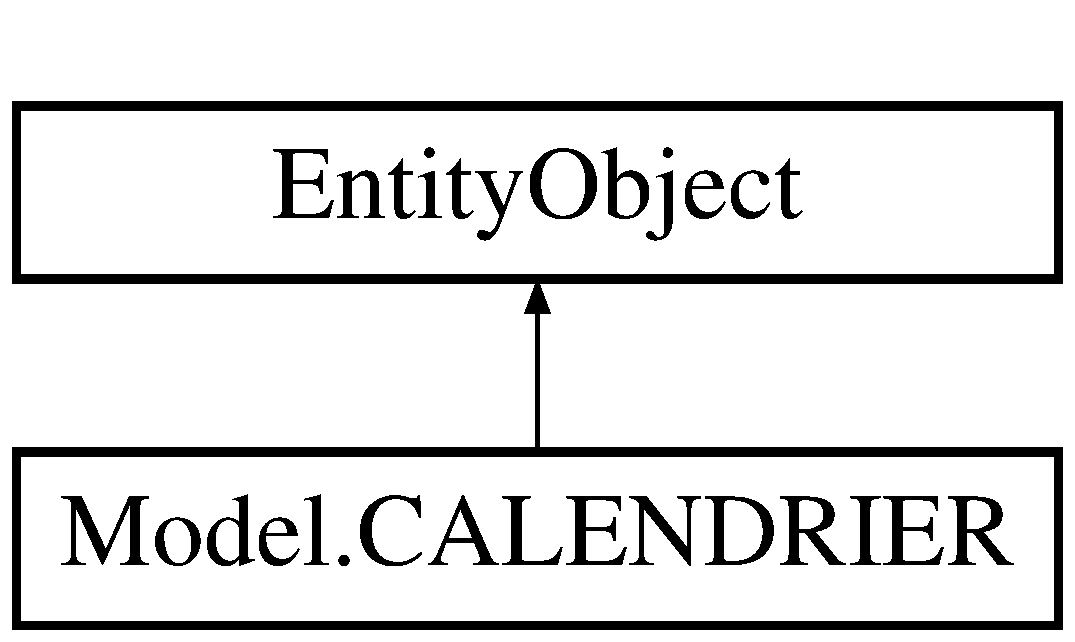
\includegraphics[height=2.000000cm]{class_model_1_1_c_a_l_e_n_d_r_i_e_r}
\end{center}
\end{figure}
\subsection*{Static Public Member Functions}
\begin{DoxyCompactItemize}
\item 
static \hyperlink{class_model_1_1_c_a_l_e_n_d_r_i_e_r}{C\-A\-L\-E\-N\-D\-R\-I\-E\-R} \hyperlink{class_model_1_1_c_a_l_e_n_d_r_i_e_r_a6f0ca13a05bde43050b45903be040a94}{Create\-C\-A\-L\-E\-N\-D\-R\-I\-E\-R} (global\-::\-System.\-Date\-Time j\-J\-M\-M\-A\-A\-A\-A\-\_\-\-D\-E\-B)
\begin{DoxyCompactList}\small\item\em Créez un nouvel objet \hyperlink{class_model_1_1_c_a_l_e_n_d_r_i_e_r}{C\-A\-L\-E\-N\-D\-R\-I\-E\-R}. \end{DoxyCompactList}\end{DoxyCompactItemize}
\subsection*{Properties}
\begin{DoxyCompactItemize}
\item 
global\-::\-System.\-Date\-Time \hyperlink{class_model_1_1_c_a_l_e_n_d_r_i_e_r_ac108f24337afda1c3aae9ad11e06706f}{J\-J\-M\-M\-A\-A\-A\-A\-\_\-\-D\-E\-B}\hspace{0.3cm}{\ttfamily  \mbox{[}get, set\mbox{]}}
\begin{DoxyCompactList}\small\item\em Aucune documentation sur les métadonnées n'est disponible. \end{DoxyCompactList}\item 
Entity\-Collection\\*
$<$ \hyperlink{class_model_1_1_e_t_r_e___r_e_s_p_o_n_s_a_b_l_e}{E\-T\-R\-E\-\_\-\-R\-E\-S\-P\-O\-N\-S\-A\-B\-L\-E} $>$ \hyperlink{class_model_1_1_c_a_l_e_n_d_r_i_e_r_a59c5b444cf3d54009756f7c4772d3a99}{E\-T\-R\-E\-\_\-\-R\-E\-S\-P\-O\-N\-S\-A\-B\-L\-E}\hspace{0.3cm}{\ttfamily  \mbox{[}get, set\mbox{]}}
\begin{DoxyCompactList}\small\item\em Aucune documentation sur les métadonnées n'est disponible. \end{DoxyCompactList}\item 
Entity\-Collection$<$ \hyperlink{class_model_1_1_g_e_r_e}{G\-E\-R\-E} $>$ \hyperlink{class_model_1_1_c_a_l_e_n_d_r_i_e_r_a0da6b33d11ac2daa1651c78a755662f1}{G\-E\-R\-E}\hspace{0.3cm}{\ttfamily  \mbox{[}get, set\mbox{]}}
\begin{DoxyCompactList}\small\item\em Aucune documentation sur les métadonnées n'est disponible. \end{DoxyCompactList}\end{DoxyCompactItemize}


\subsection{Detailed Description}
Aucune documentation sur les métadonnées n'est disponible. 



\subsection{Member Function Documentation}
\hypertarget{class_model_1_1_c_a_l_e_n_d_r_i_e_r_a6f0ca13a05bde43050b45903be040a94}{\index{Model\-::\-C\-A\-L\-E\-N\-D\-R\-I\-E\-R@{Model\-::\-C\-A\-L\-E\-N\-D\-R\-I\-E\-R}!Create\-C\-A\-L\-E\-N\-D\-R\-I\-E\-R@{Create\-C\-A\-L\-E\-N\-D\-R\-I\-E\-R}}
\index{Create\-C\-A\-L\-E\-N\-D\-R\-I\-E\-R@{Create\-C\-A\-L\-E\-N\-D\-R\-I\-E\-R}!Model::CALENDRIER@{Model\-::\-C\-A\-L\-E\-N\-D\-R\-I\-E\-R}}
\subsubsection[{Create\-C\-A\-L\-E\-N\-D\-R\-I\-E\-R}]{\setlength{\rightskip}{0pt plus 5cm}static {\bf C\-A\-L\-E\-N\-D\-R\-I\-E\-R} Model.\-C\-A\-L\-E\-N\-D\-R\-I\-E\-R.\-Create\-C\-A\-L\-E\-N\-D\-R\-I\-E\-R (
\begin{DoxyParamCaption}
\item[{global\-::\-System.\-Date\-Time}]{j\-J\-M\-M\-A\-A\-A\-A\-\_\-\-D\-E\-B}
\end{DoxyParamCaption}
)\hspace{0.3cm}{\ttfamily [static]}}}\label{class_model_1_1_c_a_l_e_n_d_r_i_e_r_a6f0ca13a05bde43050b45903be040a94}


Créez un nouvel objet \hyperlink{class_model_1_1_c_a_l_e_n_d_r_i_e_r}{C\-A\-L\-E\-N\-D\-R\-I\-E\-R}. 


\begin{DoxyParams}{Parameters}
{\em j\-J\-M\-M\-A\-A\-A\-A\-\_\-\-D\-E\-B} & Valeur initiale de la propriété J\-J\-M\-M\-A\-A\-A\-A\-\_\-\-D\-E\-B.\\
\hline
\end{DoxyParams}


\subsection{Property Documentation}
\hypertarget{class_model_1_1_c_a_l_e_n_d_r_i_e_r_a59c5b444cf3d54009756f7c4772d3a99}{\index{Model\-::\-C\-A\-L\-E\-N\-D\-R\-I\-E\-R@{Model\-::\-C\-A\-L\-E\-N\-D\-R\-I\-E\-R}!E\-T\-R\-E\-\_\-\-R\-E\-S\-P\-O\-N\-S\-A\-B\-L\-E@{E\-T\-R\-E\-\_\-\-R\-E\-S\-P\-O\-N\-S\-A\-B\-L\-E}}
\index{E\-T\-R\-E\-\_\-\-R\-E\-S\-P\-O\-N\-S\-A\-B\-L\-E@{E\-T\-R\-E\-\_\-\-R\-E\-S\-P\-O\-N\-S\-A\-B\-L\-E}!Model::CALENDRIER@{Model\-::\-C\-A\-L\-E\-N\-D\-R\-I\-E\-R}}
\subsubsection[{E\-T\-R\-E\-\_\-\-R\-E\-S\-P\-O\-N\-S\-A\-B\-L\-E}]{\setlength{\rightskip}{0pt plus 5cm}Entity\-Collection$<${\bf E\-T\-R\-E\-\_\-\-R\-E\-S\-P\-O\-N\-S\-A\-B\-L\-E}$>$ Model.\-C\-A\-L\-E\-N\-D\-R\-I\-E\-R.\-E\-T\-R\-E\-\_\-\-R\-E\-S\-P\-O\-N\-S\-A\-B\-L\-E\hspace{0.3cm}{\ttfamily [get]}, {\ttfamily [set]}}}\label{class_model_1_1_c_a_l_e_n_d_r_i_e_r_a59c5b444cf3d54009756f7c4772d3a99}


Aucune documentation sur les métadonnées n'est disponible. 

\hypertarget{class_model_1_1_c_a_l_e_n_d_r_i_e_r_a0da6b33d11ac2daa1651c78a755662f1}{\index{Model\-::\-C\-A\-L\-E\-N\-D\-R\-I\-E\-R@{Model\-::\-C\-A\-L\-E\-N\-D\-R\-I\-E\-R}!G\-E\-R\-E@{G\-E\-R\-E}}
\index{G\-E\-R\-E@{G\-E\-R\-E}!Model::CALENDRIER@{Model\-::\-C\-A\-L\-E\-N\-D\-R\-I\-E\-R}}
\subsubsection[{G\-E\-R\-E}]{\setlength{\rightskip}{0pt plus 5cm}Entity\-Collection$<${\bf G\-E\-R\-E}$>$ Model.\-C\-A\-L\-E\-N\-D\-R\-I\-E\-R.\-G\-E\-R\-E\hspace{0.3cm}{\ttfamily [get]}, {\ttfamily [set]}}}\label{class_model_1_1_c_a_l_e_n_d_r_i_e_r_a0da6b33d11ac2daa1651c78a755662f1}


Aucune documentation sur les métadonnées n'est disponible. 

\hypertarget{class_model_1_1_c_a_l_e_n_d_r_i_e_r_ac108f24337afda1c3aae9ad11e06706f}{\index{Model\-::\-C\-A\-L\-E\-N\-D\-R\-I\-E\-R@{Model\-::\-C\-A\-L\-E\-N\-D\-R\-I\-E\-R}!J\-J\-M\-M\-A\-A\-A\-A\-\_\-\-D\-E\-B@{J\-J\-M\-M\-A\-A\-A\-A\-\_\-\-D\-E\-B}}
\index{J\-J\-M\-M\-A\-A\-A\-A\-\_\-\-D\-E\-B@{J\-J\-M\-M\-A\-A\-A\-A\-\_\-\-D\-E\-B}!Model::CALENDRIER@{Model\-::\-C\-A\-L\-E\-N\-D\-R\-I\-E\-R}}
\subsubsection[{J\-J\-M\-M\-A\-A\-A\-A\-\_\-\-D\-E\-B}]{\setlength{\rightskip}{0pt plus 5cm}global.\-System.\-Date\-Time Model.\-C\-A\-L\-E\-N\-D\-R\-I\-E\-R.\-J\-J\-M\-M\-A\-A\-A\-A\-\_\-\-D\-E\-B\hspace{0.3cm}{\ttfamily [get]}, {\ttfamily [set]}}}\label{class_model_1_1_c_a_l_e_n_d_r_i_e_r_ac108f24337afda1c3aae9ad11e06706f}


Aucune documentation sur les métadonnées n'est disponible. 



The documentation for this class was generated from the following file\-:\begin{DoxyCompactItemize}
\item 
C\-:/\-Users/dju/\-Documents/\-Visual Studio 2012/\-Projects/\-P\-P\-E/\-P\-P\-E3/\-Model/\hyperlink{_model_bdd_sio_8_designer_8cs}{Model\-Bdd\-Sio.\-Designer.\-cs}\end{DoxyCompactItemize}

\hypertarget{class_wpf_application_1_1_model_1_1_client}{\section{Wpf\-Application.\-Model.\-Client Class Reference}
\label{class_wpf_application_1_1_model_1_1_client}\index{Wpf\-Application.\-Model.\-Client@{Wpf\-Application.\-Model.\-Client}}
}
\subsection*{Properties}
\begin{DoxyCompactItemize}
\item 
string \hyperlink{class_wpf_application_1_1_model_1_1_client_a3f49a129721a9bfffb482de1658c88f7}{Prenom}\hspace{0.3cm}{\ttfamily  \mbox{[}get, set\mbox{]}}
\item 
int \hyperlink{class_wpf_application_1_1_model_1_1_client_a6f8385b0794898f510b0711eb2f69d20}{Age}\hspace{0.3cm}{\ttfamily  \mbox{[}get, set\mbox{]}}
\item 
bool \hyperlink{class_wpf_application_1_1_model_1_1_client_a40ac23eaedeb2a7b54e626e0f5b205bc}{Est\-Bon\-Client}\hspace{0.3cm}{\ttfamily  \mbox{[}get, set\mbox{]}}
\end{DoxyCompactItemize}


\subsection{Property Documentation}
\hypertarget{class_wpf_application_1_1_model_1_1_client_a6f8385b0794898f510b0711eb2f69d20}{\index{Wpf\-Application\-::\-Model\-::\-Client@{Wpf\-Application\-::\-Model\-::\-Client}!Age@{Age}}
\index{Age@{Age}!WpfApplication::Model::Client@{Wpf\-Application\-::\-Model\-::\-Client}}
\subsubsection[{Age}]{\setlength{\rightskip}{0pt plus 5cm}int Wpf\-Application.\-Model.\-Client.\-Age\hspace{0.3cm}{\ttfamily [get]}, {\ttfamily [set]}}}\label{class_wpf_application_1_1_model_1_1_client_a6f8385b0794898f510b0711eb2f69d20}
\hypertarget{class_wpf_application_1_1_model_1_1_client_a40ac23eaedeb2a7b54e626e0f5b205bc}{\index{Wpf\-Application\-::\-Model\-::\-Client@{Wpf\-Application\-::\-Model\-::\-Client}!Est\-Bon\-Client@{Est\-Bon\-Client}}
\index{Est\-Bon\-Client@{Est\-Bon\-Client}!WpfApplication::Model::Client@{Wpf\-Application\-::\-Model\-::\-Client}}
\subsubsection[{Est\-Bon\-Client}]{\setlength{\rightskip}{0pt plus 5cm}bool Wpf\-Application.\-Model.\-Client.\-Est\-Bon\-Client\hspace{0.3cm}{\ttfamily [get]}, {\ttfamily [set]}}}\label{class_wpf_application_1_1_model_1_1_client_a40ac23eaedeb2a7b54e626e0f5b205bc}
\hypertarget{class_wpf_application_1_1_model_1_1_client_a3f49a129721a9bfffb482de1658c88f7}{\index{Wpf\-Application\-::\-Model\-::\-Client@{Wpf\-Application\-::\-Model\-::\-Client}!Prenom@{Prenom}}
\index{Prenom@{Prenom}!WpfApplication::Model::Client@{Wpf\-Application\-::\-Model\-::\-Client}}
\subsubsection[{Prenom}]{\setlength{\rightskip}{0pt plus 5cm}string Wpf\-Application.\-Model.\-Client.\-Prenom\hspace{0.3cm}{\ttfamily [get]}, {\ttfamily [set]}}}\label{class_wpf_application_1_1_model_1_1_client_a3f49a129721a9bfffb482de1658c88f7}


The documentation for this class was generated from the following file\-:\begin{DoxyCompactItemize}
\item 
C\-:/\-Users/dju/\-Documents/\-Visual Studio 2012/\-Projects/\-P\-P\-E/\-P\-P\-E3/\-Wpf\-Application/\-Model/\hyperlink{_client_8cs}{Client.\-cs}\end{DoxyCompactItemize}

\hypertarget{class_model_1_1helpers_1_1_col_helper}{\section{Model.\-helpers.\-Col\-Helper Class Reference}
\label{class_model_1_1helpers_1_1_col_helper}\index{Model.\-helpers.\-Col\-Helper@{Model.\-helpers.\-Col\-Helper}}
}
\subsection*{Public Member Functions}
\begin{DoxyCompactItemize}
\item 
\hyperlink{class_model_1_1helpers_1_1_col_helper_ad5b304defcf14840c15d8eca532b7c83}{Col\-Helper} ()
\item 
List$<$ \hyperlink{class_model_1_1_c_o_l_l_a_b_o_r_a_t_e_u_r}{C\-O\-L\-L\-A\-B\-O\-R\-A\-T\-E\-U\-R} $>$ \hyperlink{class_model_1_1helpers_1_1_col_helper_ac171a9c499134d6055fb8ce91ddccd52}{Get\-List} ()
\item 
\hyperlink{class_model_1_1_c_o_l_l_a_b_o_r_a_t_e_u_r}{C\-O\-L\-L\-A\-B\-O\-R\-A\-T\-E\-U\-R} \hyperlink{class_model_1_1helpers_1_1_col_helper_a581e30cc28ca598085208bce82c4388a}{Get\-One\-By\-Username} (string username)
\item 
void \hyperlink{class_model_1_1helpers_1_1_col_helper_a3d832ad4e389ffdd00eb41e94ee0dc5d}{Insert} (\hyperlink{class_model_1_1_c_o_l_l_a_b_o_r_a_t_e_u_r}{C\-O\-L\-L\-A\-B\-O\-R\-A\-T\-E\-U\-R} collaborateur)
\item 
void \hyperlink{class_model_1_1helpers_1_1_col_helper_a2d161545f0caaba88414294fd80b36e6}{Update} (\hyperlink{class_model_1_1_c_o_l_l_a_b_o_r_a_t_e_u_r}{C\-O\-L\-L\-A\-B\-O\-R\-A\-T\-E\-U\-R} collaborateur)
\item 
void \hyperlink{class_model_1_1helpers_1_1_col_helper_ad4eb731348d488e60a7e05bf4f8e60c7}{Delete} (\hyperlink{class_model_1_1_c_o_l_l_a_b_o_r_a_t_e_u_r}{C\-O\-L\-L\-A\-B\-O\-R\-A\-T\-E\-U\-R} collaborateur)
\end{DoxyCompactItemize}
\subsection*{Properties}
\begin{DoxyCompactItemize}
\item 
static \hyperlink{class_model_1_1helpers_1_1_col_helper}{Col\-Helper} \hyperlink{class_model_1_1helpers_1_1_col_helper_ac7aec6cd333abdb9d6a857fdb67330ae}{Current}\hspace{0.3cm}{\ttfamily  \mbox{[}get\mbox{]}}
\begin{DoxyCompactList}\small\item\em This is a thread-\/safe, lazy singleton. See \href{http://www.yoda.arachsys.com/csharp/singleton.html}{\tt http\-://www.\-yoda.\-arachsys.\-com/csharp/singleton.\-html} for more details about its implementation. \end{DoxyCompactList}\end{DoxyCompactItemize}


\subsection{Constructor \& Destructor Documentation}
\hypertarget{class_model_1_1helpers_1_1_col_helper_ad5b304defcf14840c15d8eca532b7c83}{\index{Model\-::helpers\-::\-Col\-Helper@{Model\-::helpers\-::\-Col\-Helper}!Col\-Helper@{Col\-Helper}}
\index{Col\-Helper@{Col\-Helper}!Model::helpers::ColHelper@{Model\-::helpers\-::\-Col\-Helper}}
\subsubsection[{Col\-Helper}]{\setlength{\rightskip}{0pt plus 5cm}Model.\-helpers.\-Col\-Helper.\-Col\-Helper (
\begin{DoxyParamCaption}
{}
\end{DoxyParamCaption}
)}}\label{class_model_1_1helpers_1_1_col_helper_ad5b304defcf14840c15d8eca532b7c83}


\subsection{Member Function Documentation}
\hypertarget{class_model_1_1helpers_1_1_col_helper_ad4eb731348d488e60a7e05bf4f8e60c7}{\index{Model\-::helpers\-::\-Col\-Helper@{Model\-::helpers\-::\-Col\-Helper}!Delete@{Delete}}
\index{Delete@{Delete}!Model::helpers::ColHelper@{Model\-::helpers\-::\-Col\-Helper}}
\subsubsection[{Delete}]{\setlength{\rightskip}{0pt plus 5cm}void Model.\-helpers.\-Col\-Helper.\-Delete (
\begin{DoxyParamCaption}
\item[{{\bf C\-O\-L\-L\-A\-B\-O\-R\-A\-T\-E\-U\-R}}]{collaborateur}
\end{DoxyParamCaption}
)}}\label{class_model_1_1helpers_1_1_col_helper_ad4eb731348d488e60a7e05bf4f8e60c7}
\hypertarget{class_model_1_1helpers_1_1_col_helper_ac171a9c499134d6055fb8ce91ddccd52}{\index{Model\-::helpers\-::\-Col\-Helper@{Model\-::helpers\-::\-Col\-Helper}!Get\-List@{Get\-List}}
\index{Get\-List@{Get\-List}!Model::helpers::ColHelper@{Model\-::helpers\-::\-Col\-Helper}}
\subsubsection[{Get\-List}]{\setlength{\rightskip}{0pt plus 5cm}List$<${\bf C\-O\-L\-L\-A\-B\-O\-R\-A\-T\-E\-U\-R}$>$ Model.\-helpers.\-Col\-Helper.\-Get\-List (
\begin{DoxyParamCaption}
{}
\end{DoxyParamCaption}
)}}\label{class_model_1_1helpers_1_1_col_helper_ac171a9c499134d6055fb8ce91ddccd52}
\hypertarget{class_model_1_1helpers_1_1_col_helper_a581e30cc28ca598085208bce82c4388a}{\index{Model\-::helpers\-::\-Col\-Helper@{Model\-::helpers\-::\-Col\-Helper}!Get\-One\-By\-Username@{Get\-One\-By\-Username}}
\index{Get\-One\-By\-Username@{Get\-One\-By\-Username}!Model::helpers::ColHelper@{Model\-::helpers\-::\-Col\-Helper}}
\subsubsection[{Get\-One\-By\-Username}]{\setlength{\rightskip}{0pt plus 5cm}{\bf C\-O\-L\-L\-A\-B\-O\-R\-A\-T\-E\-U\-R} Model.\-helpers.\-Col\-Helper.\-Get\-One\-By\-Username (
\begin{DoxyParamCaption}
\item[{string}]{username}
\end{DoxyParamCaption}
)}}\label{class_model_1_1helpers_1_1_col_helper_a581e30cc28ca598085208bce82c4388a}
\hypertarget{class_model_1_1helpers_1_1_col_helper_a3d832ad4e389ffdd00eb41e94ee0dc5d}{\index{Model\-::helpers\-::\-Col\-Helper@{Model\-::helpers\-::\-Col\-Helper}!Insert@{Insert}}
\index{Insert@{Insert}!Model::helpers::ColHelper@{Model\-::helpers\-::\-Col\-Helper}}
\subsubsection[{Insert}]{\setlength{\rightskip}{0pt plus 5cm}void Model.\-helpers.\-Col\-Helper.\-Insert (
\begin{DoxyParamCaption}
\item[{{\bf C\-O\-L\-L\-A\-B\-O\-R\-A\-T\-E\-U\-R}}]{collaborateur}
\end{DoxyParamCaption}
)}}\label{class_model_1_1helpers_1_1_col_helper_a3d832ad4e389ffdd00eb41e94ee0dc5d}
\hypertarget{class_model_1_1helpers_1_1_col_helper_a2d161545f0caaba88414294fd80b36e6}{\index{Model\-::helpers\-::\-Col\-Helper@{Model\-::helpers\-::\-Col\-Helper}!Update@{Update}}
\index{Update@{Update}!Model::helpers::ColHelper@{Model\-::helpers\-::\-Col\-Helper}}
\subsubsection[{Update}]{\setlength{\rightskip}{0pt plus 5cm}void Model.\-helpers.\-Col\-Helper.\-Update (
\begin{DoxyParamCaption}
\item[{{\bf C\-O\-L\-L\-A\-B\-O\-R\-A\-T\-E\-U\-R}}]{collaborateur}
\end{DoxyParamCaption}
)}}\label{class_model_1_1helpers_1_1_col_helper_a2d161545f0caaba88414294fd80b36e6}


\subsection{Property Documentation}
\hypertarget{class_model_1_1helpers_1_1_col_helper_ac7aec6cd333abdb9d6a857fdb67330ae}{\index{Model\-::helpers\-::\-Col\-Helper@{Model\-::helpers\-::\-Col\-Helper}!Current@{Current}}
\index{Current@{Current}!Model::helpers::ColHelper@{Model\-::helpers\-::\-Col\-Helper}}
\subsubsection[{Current}]{\setlength{\rightskip}{0pt plus 5cm}{\bf Col\-Helper} Model.\-helpers.\-Col\-Helper.\-Current\hspace{0.3cm}{\ttfamily [static]}, {\ttfamily [get]}}}\label{class_model_1_1helpers_1_1_col_helper_ac7aec6cd333abdb9d6a857fdb67330ae}


This is a thread-\/safe, lazy singleton. See \href{http://www.yoda.arachsys.com/csharp/singleton.html}{\tt http\-://www.\-yoda.\-arachsys.\-com/csharp/singleton.\-html} for more details about its implementation. 



The documentation for this class was generated from the following file\-:\begin{DoxyCompactItemize}
\item 
C\-:/\-Users/dju/\-Documents/\-Visual Studio 2012/\-Projects/\-P\-P\-E/\-P\-P\-E3/\-Model/helpers/\hyperlink{_col_helper_8cs}{Col\-Helper.\-cs}\end{DoxyCompactItemize}

\hypertarget{class_model_1_1_c_o_l_l_a_b_o_r_a_t_e_u_r}{\section{Model.\-C\-O\-L\-L\-A\-B\-O\-R\-A\-T\-E\-U\-R Class Reference}
\label{class_model_1_1_c_o_l_l_a_b_o_r_a_t_e_u_r}\index{Model.\-C\-O\-L\-L\-A\-B\-O\-R\-A\-T\-E\-U\-R@{Model.\-C\-O\-L\-L\-A\-B\-O\-R\-A\-T\-E\-U\-R}}
}


Aucune documentation sur les métadonnées n'est disponible.  


Inheritance diagram for Model.\-C\-O\-L\-L\-A\-B\-O\-R\-A\-T\-E\-U\-R\-:\begin{figure}[H]
\begin{center}
\leavevmode
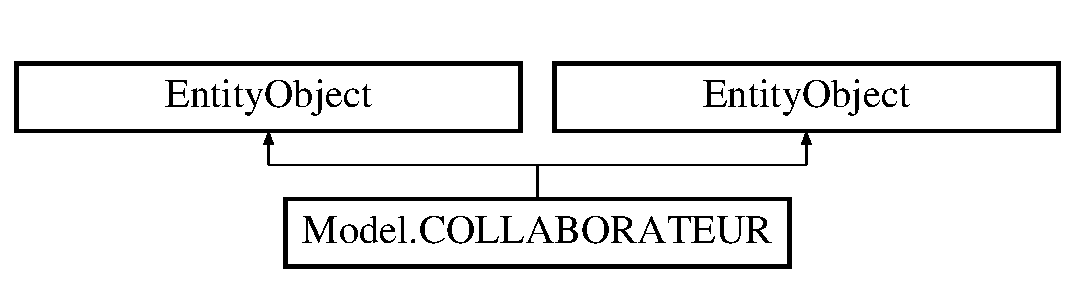
\includegraphics[height=2.000000cm]{class_model_1_1_c_o_l_l_a_b_o_r_a_t_e_u_r}
\end{center}
\end{figure}
\subsection*{Public Member Functions}
\begin{DoxyCompactItemize}
\item 
override string \hyperlink{class_model_1_1_c_o_l_l_a_b_o_r_a_t_e_u_r_add667e8008b34fe3e807452e8bfa6ef0}{To\-String} ()
\end{DoxyCompactItemize}
\subsection*{Static Public Member Functions}
\begin{DoxyCompactItemize}
\item 
static \hyperlink{class_model_1_1_c_o_l_l_a_b_o_r_a_t_e_u_r}{C\-O\-L\-L\-A\-B\-O\-R\-A\-T\-E\-U\-R} \hyperlink{class_model_1_1_c_o_l_l_a_b_o_r_a_t_e_u_r_a47fd17271ba7b48a0ab533fe4d56cd3c}{Create\-C\-O\-L\-L\-A\-B\-O\-R\-A\-T\-E\-U\-R} (global\-::\-System.\-Int32 \hyperlink{class_model_1_1_c_o_l_l_a_b_o_r_a_t_e_u_r_a1d528bb5e6dab9aee87ec0498efce970}{matricule\-\_\-col}, global\-::\-System.\-String \hyperlink{class_model_1_1_c_o_l_l_a_b_o_r_a_t_e_u_r_a16da434fc2d5fd237a9c10011c7240ad}{nom\-\_\-col}, global\-::\-System.\-String \hyperlink{class_model_1_1_c_o_l_l_a_b_o_r_a_t_e_u_r_a653654accc486107577cbe805db1e1dc}{prenom\-\_\-col}, global\-::\-System.\-String \hyperlink{class_model_1_1_c_o_l_l_a_b_o_r_a_t_e_u_r_a3a3c271af8a2fa7f9d2d8f5600fb8e56}{adresse\-\_\-col}, global\-::\-System.\-String \hyperlink{class_model_1_1_c_o_l_l_a_b_o_r_a_t_e_u_r_a264f8faf4646f7748ff732d79a4e54fd}{cp\-\_\-col}, global\-::\-System.\-String \hyperlink{class_model_1_1_c_o_l_l_a_b_o_r_a_t_e_u_r_a2099c578d33f2851b0a914aeca8a3234}{mdp\-\_\-col}, global\-::\-System.\-Date\-Time \hyperlink{class_model_1_1_c_o_l_l_a_b_o_r_a_t_e_u_r_afa00e01e2baf6b90075dd32abfd0b72f}{date\-\_\-embauche}, global\-::\-System.\-String \hyperlink{class_model_1_1_c_o_l_l_a_b_o_r_a_t_e_u_r_a52fce134f10bc131943353de60abd8cf}{ville\-\_\-col}, global\-::\-System.\-String \hyperlink{class_model_1_1_c_o_l_l_a_b_o_r_a_t_e_u_r_ae5aa55abe9ea993f8533e563a91485e0}{salt\-\_\-col})
\begin{DoxyCompactList}\small\item\em Créez un nouvel objet \hyperlink{class_model_1_1_c_o_l_l_a_b_o_r_a_t_e_u_r}{C\-O\-L\-L\-A\-B\-O\-R\-A\-T\-E\-U\-R}. \end{DoxyCompactList}\end{DoxyCompactItemize}
\subsection*{Properties}
\begin{DoxyCompactItemize}
\item 
global\-::\-System.\-Int32 \hyperlink{class_model_1_1_c_o_l_l_a_b_o_r_a_t_e_u_r_a1d528bb5e6dab9aee87ec0498efce970}{matricule\-\_\-col}\hspace{0.3cm}{\ttfamily  \mbox{[}get, set\mbox{]}}
\begin{DoxyCompactList}\small\item\em Aucune documentation sur les métadonnées n'est disponible. \end{DoxyCompactList}\item 
global\-::\-System.\-String \hyperlink{class_model_1_1_c_o_l_l_a_b_o_r_a_t_e_u_r_a16da434fc2d5fd237a9c10011c7240ad}{nom\-\_\-col}\hspace{0.3cm}{\ttfamily  \mbox{[}get, set\mbox{]}}
\begin{DoxyCompactList}\small\item\em Aucune documentation sur les métadonnées n'est disponible. \end{DoxyCompactList}\item 
global\-::\-System.\-String \hyperlink{class_model_1_1_c_o_l_l_a_b_o_r_a_t_e_u_r_a653654accc486107577cbe805db1e1dc}{prenom\-\_\-col}\hspace{0.3cm}{\ttfamily  \mbox{[}get, set\mbox{]}}
\begin{DoxyCompactList}\small\item\em Aucune documentation sur les métadonnées n'est disponible. \end{DoxyCompactList}\item 
global\-::\-System.\-String \hyperlink{class_model_1_1_c_o_l_l_a_b_o_r_a_t_e_u_r_a3a3c271af8a2fa7f9d2d8f5600fb8e56}{adresse\-\_\-col}\hspace{0.3cm}{\ttfamily  \mbox{[}get, set\mbox{]}}
\begin{DoxyCompactList}\small\item\em Aucune documentation sur les métadonnées n'est disponible. \end{DoxyCompactList}\item 
global\-::\-System.\-String \hyperlink{class_model_1_1_c_o_l_l_a_b_o_r_a_t_e_u_r_a264f8faf4646f7748ff732d79a4e54fd}{cp\-\_\-col}\hspace{0.3cm}{\ttfamily  \mbox{[}get, set\mbox{]}}
\begin{DoxyCompactList}\small\item\em Aucune documentation sur les métadonnées n'est disponible. \end{DoxyCompactList}\item 
global\-::\-System.\-String \hyperlink{class_model_1_1_c_o_l_l_a_b_o_r_a_t_e_u_r_a2099c578d33f2851b0a914aeca8a3234}{mdp\-\_\-col}\hspace{0.3cm}{\ttfamily  \mbox{[}get, set\mbox{]}}
\begin{DoxyCompactList}\small\item\em Aucune documentation sur les métadonnées n'est disponible. \end{DoxyCompactList}\item 
global\-::\-System.\-Date\-Time \hyperlink{class_model_1_1_c_o_l_l_a_b_o_r_a_t_e_u_r_afa00e01e2baf6b90075dd32abfd0b72f}{date\-\_\-embauche}\hspace{0.3cm}{\ttfamily  \mbox{[}get, set\mbox{]}}
\begin{DoxyCompactList}\small\item\em Aucune documentation sur les métadonnées n'est disponible. \end{DoxyCompactList}\item 
global\-::\-System.\-String \hyperlink{class_model_1_1_c_o_l_l_a_b_o_r_a_t_e_u_r_a52fce134f10bc131943353de60abd8cf}{ville\-\_\-col}\hspace{0.3cm}{\ttfamily  \mbox{[}get, set\mbox{]}}
\begin{DoxyCompactList}\small\item\em Aucune documentation sur les métadonnées n'est disponible. \end{DoxyCompactList}\item 
global\-::\-System.\-String \hyperlink{class_model_1_1_c_o_l_l_a_b_o_r_a_t_e_u_r_ae5aa55abe9ea993f8533e563a91485e0}{salt\-\_\-col}\hspace{0.3cm}{\ttfamily  \mbox{[}get, set\mbox{]}}
\begin{DoxyCompactList}\small\item\em Aucune documentation sur les métadonnées n'est disponible. \end{DoxyCompactList}\item 
Entity\-Collection\\*
$<$ \hyperlink{class_model_1_1_a_c_t_i_v_i_t_e___c_o_m_p_l_e_m_e_n_t_a_i_r_e}{A\-C\-T\-I\-V\-I\-T\-E\-\_\-\-C\-O\-M\-P\-L\-E\-M\-E\-N\-T\-A\-I\-R\-E} $>$ \hyperlink{class_model_1_1_c_o_l_l_a_b_o_r_a_t_e_u_r_a59cd341498640349d6b9ea0c8ade35e1}{A\-C\-T\-I\-V\-I\-T\-E\-\_\-\-C\-O\-M\-P\-L\-E\-M\-E\-N\-T\-A\-I\-R\-E}\hspace{0.3cm}{\ttfamily  \mbox{[}get, set\mbox{]}}
\begin{DoxyCompactList}\small\item\em Aucune documentation sur les métadonnées n'est disponible. \end{DoxyCompactList}\item 
\hyperlink{class_model_1_1_r_e_s_p_o_n_s_a_b_l_e___d_e___s_e_c_t_e_u_r}{R\-E\-S\-P\-O\-N\-S\-A\-B\-L\-E\-\_\-\-D\-E\-\_\-\-S\-E\-C\-T\-E\-U\-R} \hyperlink{class_model_1_1_c_o_l_l_a_b_o_r_a_t_e_u_r_a6bd320a8198906e4cfadc9427bf6e351}{R\-E\-S\-P\-O\-N\-S\-A\-B\-L\-E\-\_\-\-D\-E\-\_\-\-S\-E\-C\-T\-E\-U\-R}\hspace{0.3cm}{\ttfamily  \mbox{[}get, set\mbox{]}}
\begin{DoxyCompactList}\small\item\em Aucune documentation sur les métadonnées n'est disponible. \end{DoxyCompactList}\item 
Entity\-Reference\\*
$<$ \hyperlink{class_model_1_1_r_e_s_p_o_n_s_a_b_l_e___d_e___s_e_c_t_e_u_r}{R\-E\-S\-P\-O\-N\-S\-A\-B\-L\-E\-\_\-\-D\-E\-\_\-\-S\-E\-C\-T\-E\-U\-R} $>$ \hyperlink{class_model_1_1_c_o_l_l_a_b_o_r_a_t_e_u_r_a9a393db2beea3bd82c900349c146cffd}{R\-E\-S\-P\-O\-N\-S\-A\-B\-L\-E\-\_\-\-D\-E\-\_\-\-S\-E\-C\-T\-E\-U\-R\-Reference}\hspace{0.3cm}{\ttfamily  \mbox{[}get, set\mbox{]}}
\begin{DoxyCompactList}\small\item\em Aucune documentation sur les métadonnées n'est disponible. \end{DoxyCompactList}\item 
Entity\-Collection\\*
$<$ \hyperlink{class_model_1_1_e_t_r_e___r_e_s_p_o_n_s_a_b_l_e}{E\-T\-R\-E\-\_\-\-R\-E\-S\-P\-O\-N\-S\-A\-B\-L\-E} $>$ \hyperlink{class_model_1_1_c_o_l_l_a_b_o_r_a_t_e_u_r_a320ee68fff653feb60dfebf5665fb8e0}{E\-T\-R\-E\-\_\-\-R\-E\-S\-P\-O\-N\-S\-A\-B\-L\-E}\hspace{0.3cm}{\ttfamily  \mbox{[}get, set\mbox{]}}
\begin{DoxyCompactList}\small\item\em Aucune documentation sur les métadonnées n'est disponible. \end{DoxyCompactList}\item 
\hyperlink{class_model_1_1_d_i_r_e_c_t_e_u_r___r_e_g_i_o_n_a_l}{D\-I\-R\-E\-C\-T\-E\-U\-R\-\_\-\-R\-E\-G\-I\-O\-N\-A\-L} \hyperlink{class_model_1_1_c_o_l_l_a_b_o_r_a_t_e_u_r_a62ee9e9f4ad746037e8d90abc144bcc0}{D\-I\-R\-E\-C\-T\-E\-U\-R\-\_\-\-R\-E\-G\-I\-O\-N\-A\-L}\hspace{0.3cm}{\ttfamily  \mbox{[}get, set\mbox{]}}
\begin{DoxyCompactList}\small\item\em Aucune documentation sur les métadonnées n'est disponible. \end{DoxyCompactList}\item 
Entity\-Reference\\*
$<$ \hyperlink{class_model_1_1_d_i_r_e_c_t_e_u_r___r_e_g_i_o_n_a_l}{D\-I\-R\-E\-C\-T\-E\-U\-R\-\_\-\-R\-E\-G\-I\-O\-N\-A\-L} $>$ \hyperlink{class_model_1_1_c_o_l_l_a_b_o_r_a_t_e_u_r_a3afe8c2d48548ecbb9b2ec038bf71824}{D\-I\-R\-E\-C\-T\-E\-U\-R\-\_\-\-R\-E\-G\-I\-O\-N\-A\-L\-Reference}\hspace{0.3cm}{\ttfamily  \mbox{[}get, set\mbox{]}}
\begin{DoxyCompactList}\small\item\em Aucune documentation sur les métadonnées n'est disponible. \end{DoxyCompactList}\item 
\hyperlink{class_model_1_1_v_i_s_i_t_e_u_r}{V\-I\-S\-I\-T\-E\-U\-R} \hyperlink{class_model_1_1_c_o_l_l_a_b_o_r_a_t_e_u_r_a26d90f7ca8e82c6068ce5b62edf893c5}{V\-I\-S\-I\-T\-E\-U\-R}\hspace{0.3cm}{\ttfamily  \mbox{[}get, set\mbox{]}}
\begin{DoxyCompactList}\small\item\em Aucune documentation sur les métadonnées n'est disponible. \end{DoxyCompactList}\item 
Entity\-Reference$<$ \hyperlink{class_model_1_1_v_i_s_i_t_e_u_r}{V\-I\-S\-I\-T\-E\-U\-R} $>$ \hyperlink{class_model_1_1_c_o_l_l_a_b_o_r_a_t_e_u_r_a480fc3f4e938e8e0211622b9f6d4dd14}{V\-I\-S\-I\-T\-E\-U\-R\-Reference}\hspace{0.3cm}{\ttfamily  \mbox{[}get, set\mbox{]}}
\begin{DoxyCompactList}\small\item\em Aucune documentation sur les métadonnées n'est disponible. \end{DoxyCompactList}\item 
Entity\-Collection$<$ \hyperlink{class_model_1_1_f_i_c_h_e___f_r_a_i_s}{F\-I\-C\-H\-E\-\_\-\-F\-R\-A\-I\-S} $>$ \hyperlink{class_model_1_1_c_o_l_l_a_b_o_r_a_t_e_u_r_a22af8667a48d207688fa85b70ae69b62}{F\-I\-C\-H\-E\-\_\-\-F\-R\-A\-I\-S}\hspace{0.3cm}{\ttfamily  \mbox{[}get, set\mbox{]}}
\begin{DoxyCompactList}\small\item\em Aucune documentation sur les métadonnées n'est disponible. \end{DoxyCompactList}\item 
Entity\-Collection$<$ \hyperlink{class_model_1_1_g_e_r_e}{G\-E\-R\-E} $>$ \hyperlink{class_model_1_1_c_o_l_l_a_b_o_r_a_t_e_u_r_a09aa4348c01e391b24c2ec4134060e0b}{G\-E\-R\-E}\hspace{0.3cm}{\ttfamily  \mbox{[}get, set\mbox{]}}
\begin{DoxyCompactList}\small\item\em Aucune documentation sur les métadonnées n'est disponible. \end{DoxyCompactList}\item 
Entity\-Collection\\*
$<$ \hyperlink{class_model_1_1_a_c_t_i_v_i_t_e___c_o_m_p_l_e_m_e_n_t_a_i_r_e}{A\-C\-T\-I\-V\-I\-T\-E\-\_\-\-C\-O\-M\-P\-L\-E\-M\-E\-N\-T\-A\-I\-R\-E} $>$ \hyperlink{class_model_1_1_c_o_l_l_a_b_o_r_a_t_e_u_r_a7dafc5bd0e0a0e4d1c605ceb365154f8}{A\-C\-T\-I\-V\-I\-T\-E\-\_\-\-C\-O\-M\-P\-L\-E\-M\-E\-N\-T\-A\-I\-R\-E1}\hspace{0.3cm}{\ttfamily  \mbox{[}get, set\mbox{]}}
\begin{DoxyCompactList}\small\item\em Aucune documentation sur les métadonnées n'est disponible. \end{DoxyCompactList}\item 
Entity\-Collection\\*
$<$ \hyperlink{class_model_1_1_r_a_p_p_o_r_t___d_e___v_i_s_i_t_e}{R\-A\-P\-P\-O\-R\-T\-\_\-\-D\-E\-\_\-\-V\-I\-S\-I\-T\-E} $>$ \hyperlink{class_model_1_1_c_o_l_l_a_b_o_r_a_t_e_u_r_ad416f8f8000aecc56d0e0ed3be701852}{R\-A\-P\-P\-O\-R\-T\-\_\-\-D\-E\-\_\-\-V\-I\-S\-I\-T\-E}\hspace{0.3cm}{\ttfamily  \mbox{[}get, set\mbox{]}}
\begin{DoxyCompactList}\small\item\em Aucune documentation sur les métadonnées n'est disponible. \end{DoxyCompactList}\item 
Entity\-Collection$<$ \hyperlink{class_model_1_1_a_v_o_i_r1}{A\-V\-O\-I\-R1} $>$ \hyperlink{class_model_1_1_c_o_l_l_a_b_o_r_a_t_e_u_r_a948323a5e1d10ad783ec22e2a42b9a67}{A\-V\-O\-I\-R}\hspace{0.3cm}{\ttfamily  \mbox{[}get, set\mbox{]}}
\begin{DoxyCompactList}\small\item\em Aucune documentation sur les métadonnées n'est disponible. \end{DoxyCompactList}\end{DoxyCompactItemize}


\subsection{Detailed Description}
Aucune documentation sur les métadonnées n'est disponible. 



\subsection{Member Function Documentation}
\hypertarget{class_model_1_1_c_o_l_l_a_b_o_r_a_t_e_u_r_a47fd17271ba7b48a0ab533fe4d56cd3c}{\index{Model\-::\-C\-O\-L\-L\-A\-B\-O\-R\-A\-T\-E\-U\-R@{Model\-::\-C\-O\-L\-L\-A\-B\-O\-R\-A\-T\-E\-U\-R}!Create\-C\-O\-L\-L\-A\-B\-O\-R\-A\-T\-E\-U\-R@{Create\-C\-O\-L\-L\-A\-B\-O\-R\-A\-T\-E\-U\-R}}
\index{Create\-C\-O\-L\-L\-A\-B\-O\-R\-A\-T\-E\-U\-R@{Create\-C\-O\-L\-L\-A\-B\-O\-R\-A\-T\-E\-U\-R}!Model::COLLABORATEUR@{Model\-::\-C\-O\-L\-L\-A\-B\-O\-R\-A\-T\-E\-U\-R}}
\subsubsection[{Create\-C\-O\-L\-L\-A\-B\-O\-R\-A\-T\-E\-U\-R}]{\setlength{\rightskip}{0pt plus 5cm}static {\bf C\-O\-L\-L\-A\-B\-O\-R\-A\-T\-E\-U\-R} Model.\-C\-O\-L\-L\-A\-B\-O\-R\-A\-T\-E\-U\-R.\-Create\-C\-O\-L\-L\-A\-B\-O\-R\-A\-T\-E\-U\-R (
\begin{DoxyParamCaption}
\item[{global\-::\-System.\-Int32}]{matricule\-\_\-col, }
\item[{global\-::\-System.\-String}]{nom\-\_\-col, }
\item[{global\-::\-System.\-String}]{prenom\-\_\-col, }
\item[{global\-::\-System.\-String}]{adresse\-\_\-col, }
\item[{global\-::\-System.\-String}]{cp\-\_\-col, }
\item[{global\-::\-System.\-String}]{mdp\-\_\-col, }
\item[{global\-::\-System.\-Date\-Time}]{date\-\_\-embauche, }
\item[{global\-::\-System.\-String}]{ville\-\_\-col, }
\item[{global\-::\-System.\-String}]{salt\-\_\-col}
\end{DoxyParamCaption}
)\hspace{0.3cm}{\ttfamily [static]}}}\label{class_model_1_1_c_o_l_l_a_b_o_r_a_t_e_u_r_a47fd17271ba7b48a0ab533fe4d56cd3c}


Créez un nouvel objet \hyperlink{class_model_1_1_c_o_l_l_a_b_o_r_a_t_e_u_r}{C\-O\-L\-L\-A\-B\-O\-R\-A\-T\-E\-U\-R}. 


\begin{DoxyParams}{Parameters}
{\em matricule\-\_\-col} & Valeur initiale de la propriété matricule\-\_\-col.\\
\hline
{\em nom\-\_\-col} & Valeur initiale de la propriété nom\-\_\-col.\\
\hline
{\em prenom\-\_\-col} & Valeur initiale de la propriété prenom\-\_\-col.\\
\hline
{\em adresse\-\_\-col} & Valeur initiale de la propriété adresse\-\_\-col.\\
\hline
{\em cp\-\_\-col} & Valeur initiale de la propriété cp\-\_\-col.\\
\hline
{\em mdp\-\_\-col} & Valeur initiale de la propriété mdp\-\_\-col.\\
\hline
{\em date\-\_\-embauche} & Valeur initiale de la propriété date\-\_\-embauche.\\
\hline
{\em ville\-\_\-col} & Valeur initiale de la propriété ville\-\_\-col.\\
\hline
{\em salt\-\_\-col} & Valeur initiale de la propriété salt\-\_\-col.\\
\hline
\end{DoxyParams}
\hypertarget{class_model_1_1_c_o_l_l_a_b_o_r_a_t_e_u_r_add667e8008b34fe3e807452e8bfa6ef0}{\index{Model\-::\-C\-O\-L\-L\-A\-B\-O\-R\-A\-T\-E\-U\-R@{Model\-::\-C\-O\-L\-L\-A\-B\-O\-R\-A\-T\-E\-U\-R}!To\-String@{To\-String}}
\index{To\-String@{To\-String}!Model::COLLABORATEUR@{Model\-::\-C\-O\-L\-L\-A\-B\-O\-R\-A\-T\-E\-U\-R}}
\subsubsection[{To\-String}]{\setlength{\rightskip}{0pt plus 5cm}override string Model.\-C\-O\-L\-L\-A\-B\-O\-R\-A\-T\-E\-U\-R.\-To\-String (
\begin{DoxyParamCaption}
{}
\end{DoxyParamCaption}
)}}\label{class_model_1_1_c_o_l_l_a_b_o_r_a_t_e_u_r_add667e8008b34fe3e807452e8bfa6ef0}


\subsection{Property Documentation}
\hypertarget{class_model_1_1_c_o_l_l_a_b_o_r_a_t_e_u_r_a59cd341498640349d6b9ea0c8ade35e1}{\index{Model\-::\-C\-O\-L\-L\-A\-B\-O\-R\-A\-T\-E\-U\-R@{Model\-::\-C\-O\-L\-L\-A\-B\-O\-R\-A\-T\-E\-U\-R}!A\-C\-T\-I\-V\-I\-T\-E\-\_\-\-C\-O\-M\-P\-L\-E\-M\-E\-N\-T\-A\-I\-R\-E@{A\-C\-T\-I\-V\-I\-T\-E\-\_\-\-C\-O\-M\-P\-L\-E\-M\-E\-N\-T\-A\-I\-R\-E}}
\index{A\-C\-T\-I\-V\-I\-T\-E\-\_\-\-C\-O\-M\-P\-L\-E\-M\-E\-N\-T\-A\-I\-R\-E@{A\-C\-T\-I\-V\-I\-T\-E\-\_\-\-C\-O\-M\-P\-L\-E\-M\-E\-N\-T\-A\-I\-R\-E}!Model::COLLABORATEUR@{Model\-::\-C\-O\-L\-L\-A\-B\-O\-R\-A\-T\-E\-U\-R}}
\subsubsection[{A\-C\-T\-I\-V\-I\-T\-E\-\_\-\-C\-O\-M\-P\-L\-E\-M\-E\-N\-T\-A\-I\-R\-E}]{\setlength{\rightskip}{0pt plus 5cm}Entity\-Collection$<${\bf A\-C\-T\-I\-V\-I\-T\-E\-\_\-\-C\-O\-M\-P\-L\-E\-M\-E\-N\-T\-A\-I\-R\-E}$>$ Model.\-C\-O\-L\-L\-A\-B\-O\-R\-A\-T\-E\-U\-R.\-A\-C\-T\-I\-V\-I\-T\-E\-\_\-\-C\-O\-M\-P\-L\-E\-M\-E\-N\-T\-A\-I\-R\-E\hspace{0.3cm}{\ttfamily [get]}, {\ttfamily [set]}}}\label{class_model_1_1_c_o_l_l_a_b_o_r_a_t_e_u_r_a59cd341498640349d6b9ea0c8ade35e1}


Aucune documentation sur les métadonnées n'est disponible. 

\hypertarget{class_model_1_1_c_o_l_l_a_b_o_r_a_t_e_u_r_a7dafc5bd0e0a0e4d1c605ceb365154f8}{\index{Model\-::\-C\-O\-L\-L\-A\-B\-O\-R\-A\-T\-E\-U\-R@{Model\-::\-C\-O\-L\-L\-A\-B\-O\-R\-A\-T\-E\-U\-R}!A\-C\-T\-I\-V\-I\-T\-E\-\_\-\-C\-O\-M\-P\-L\-E\-M\-E\-N\-T\-A\-I\-R\-E1@{A\-C\-T\-I\-V\-I\-T\-E\-\_\-\-C\-O\-M\-P\-L\-E\-M\-E\-N\-T\-A\-I\-R\-E1}}
\index{A\-C\-T\-I\-V\-I\-T\-E\-\_\-\-C\-O\-M\-P\-L\-E\-M\-E\-N\-T\-A\-I\-R\-E1@{A\-C\-T\-I\-V\-I\-T\-E\-\_\-\-C\-O\-M\-P\-L\-E\-M\-E\-N\-T\-A\-I\-R\-E1}!Model::COLLABORATEUR@{Model\-::\-C\-O\-L\-L\-A\-B\-O\-R\-A\-T\-E\-U\-R}}
\subsubsection[{A\-C\-T\-I\-V\-I\-T\-E\-\_\-\-C\-O\-M\-P\-L\-E\-M\-E\-N\-T\-A\-I\-R\-E1}]{\setlength{\rightskip}{0pt plus 5cm}Entity\-Collection$<${\bf A\-C\-T\-I\-V\-I\-T\-E\-\_\-\-C\-O\-M\-P\-L\-E\-M\-E\-N\-T\-A\-I\-R\-E}$>$ Model.\-C\-O\-L\-L\-A\-B\-O\-R\-A\-T\-E\-U\-R.\-A\-C\-T\-I\-V\-I\-T\-E\-\_\-\-C\-O\-M\-P\-L\-E\-M\-E\-N\-T\-A\-I\-R\-E1\hspace{0.3cm}{\ttfamily [get]}, {\ttfamily [set]}}}\label{class_model_1_1_c_o_l_l_a_b_o_r_a_t_e_u_r_a7dafc5bd0e0a0e4d1c605ceb365154f8}


Aucune documentation sur les métadonnées n'est disponible. 

\hypertarget{class_model_1_1_c_o_l_l_a_b_o_r_a_t_e_u_r_a3a3c271af8a2fa7f9d2d8f5600fb8e56}{\index{Model\-::\-C\-O\-L\-L\-A\-B\-O\-R\-A\-T\-E\-U\-R@{Model\-::\-C\-O\-L\-L\-A\-B\-O\-R\-A\-T\-E\-U\-R}!adresse\-\_\-col@{adresse\-\_\-col}}
\index{adresse\-\_\-col@{adresse\-\_\-col}!Model::COLLABORATEUR@{Model\-::\-C\-O\-L\-L\-A\-B\-O\-R\-A\-T\-E\-U\-R}}
\subsubsection[{adresse\-\_\-col}]{\setlength{\rightskip}{0pt plus 5cm}global.\-System.\-String Model.\-C\-O\-L\-L\-A\-B\-O\-R\-A\-T\-E\-U\-R.\-adresse\-\_\-col\hspace{0.3cm}{\ttfamily [get]}, {\ttfamily [set]}}}\label{class_model_1_1_c_o_l_l_a_b_o_r_a_t_e_u_r_a3a3c271af8a2fa7f9d2d8f5600fb8e56}


Aucune documentation sur les métadonnées n'est disponible. 

\hypertarget{class_model_1_1_c_o_l_l_a_b_o_r_a_t_e_u_r_a948323a5e1d10ad783ec22e2a42b9a67}{\index{Model\-::\-C\-O\-L\-L\-A\-B\-O\-R\-A\-T\-E\-U\-R@{Model\-::\-C\-O\-L\-L\-A\-B\-O\-R\-A\-T\-E\-U\-R}!A\-V\-O\-I\-R@{A\-V\-O\-I\-R}}
\index{A\-V\-O\-I\-R@{A\-V\-O\-I\-R}!Model::COLLABORATEUR@{Model\-::\-C\-O\-L\-L\-A\-B\-O\-R\-A\-T\-E\-U\-R}}
\subsubsection[{A\-V\-O\-I\-R}]{\setlength{\rightskip}{0pt plus 5cm}Entity\-Collection$<${\bf A\-V\-O\-I\-R1}$>$ Model.\-C\-O\-L\-L\-A\-B\-O\-R\-A\-T\-E\-U\-R.\-A\-V\-O\-I\-R\hspace{0.3cm}{\ttfamily [get]}, {\ttfamily [set]}}}\label{class_model_1_1_c_o_l_l_a_b_o_r_a_t_e_u_r_a948323a5e1d10ad783ec22e2a42b9a67}


Aucune documentation sur les métadonnées n'est disponible. 

\hypertarget{class_model_1_1_c_o_l_l_a_b_o_r_a_t_e_u_r_a264f8faf4646f7748ff732d79a4e54fd}{\index{Model\-::\-C\-O\-L\-L\-A\-B\-O\-R\-A\-T\-E\-U\-R@{Model\-::\-C\-O\-L\-L\-A\-B\-O\-R\-A\-T\-E\-U\-R}!cp\-\_\-col@{cp\-\_\-col}}
\index{cp\-\_\-col@{cp\-\_\-col}!Model::COLLABORATEUR@{Model\-::\-C\-O\-L\-L\-A\-B\-O\-R\-A\-T\-E\-U\-R}}
\subsubsection[{cp\-\_\-col}]{\setlength{\rightskip}{0pt plus 5cm}global.\-System.\-String Model.\-C\-O\-L\-L\-A\-B\-O\-R\-A\-T\-E\-U\-R.\-cp\-\_\-col\hspace{0.3cm}{\ttfamily [get]}, {\ttfamily [set]}}}\label{class_model_1_1_c_o_l_l_a_b_o_r_a_t_e_u_r_a264f8faf4646f7748ff732d79a4e54fd}


Aucune documentation sur les métadonnées n'est disponible. 

\hypertarget{class_model_1_1_c_o_l_l_a_b_o_r_a_t_e_u_r_afa00e01e2baf6b90075dd32abfd0b72f}{\index{Model\-::\-C\-O\-L\-L\-A\-B\-O\-R\-A\-T\-E\-U\-R@{Model\-::\-C\-O\-L\-L\-A\-B\-O\-R\-A\-T\-E\-U\-R}!date\-\_\-embauche@{date\-\_\-embauche}}
\index{date\-\_\-embauche@{date\-\_\-embauche}!Model::COLLABORATEUR@{Model\-::\-C\-O\-L\-L\-A\-B\-O\-R\-A\-T\-E\-U\-R}}
\subsubsection[{date\-\_\-embauche}]{\setlength{\rightskip}{0pt plus 5cm}global.\-System.\-Date\-Time Model.\-C\-O\-L\-L\-A\-B\-O\-R\-A\-T\-E\-U\-R.\-date\-\_\-embauche\hspace{0.3cm}{\ttfamily [get]}, {\ttfamily [set]}}}\label{class_model_1_1_c_o_l_l_a_b_o_r_a_t_e_u_r_afa00e01e2baf6b90075dd32abfd0b72f}


Aucune documentation sur les métadonnées n'est disponible. 

\hypertarget{class_model_1_1_c_o_l_l_a_b_o_r_a_t_e_u_r_a62ee9e9f4ad746037e8d90abc144bcc0}{\index{Model\-::\-C\-O\-L\-L\-A\-B\-O\-R\-A\-T\-E\-U\-R@{Model\-::\-C\-O\-L\-L\-A\-B\-O\-R\-A\-T\-E\-U\-R}!D\-I\-R\-E\-C\-T\-E\-U\-R\-\_\-\-R\-E\-G\-I\-O\-N\-A\-L@{D\-I\-R\-E\-C\-T\-E\-U\-R\-\_\-\-R\-E\-G\-I\-O\-N\-A\-L}}
\index{D\-I\-R\-E\-C\-T\-E\-U\-R\-\_\-\-R\-E\-G\-I\-O\-N\-A\-L@{D\-I\-R\-E\-C\-T\-E\-U\-R\-\_\-\-R\-E\-G\-I\-O\-N\-A\-L}!Model::COLLABORATEUR@{Model\-::\-C\-O\-L\-L\-A\-B\-O\-R\-A\-T\-E\-U\-R}}
\subsubsection[{D\-I\-R\-E\-C\-T\-E\-U\-R\-\_\-\-R\-E\-G\-I\-O\-N\-A\-L}]{\setlength{\rightskip}{0pt plus 5cm}{\bf D\-I\-R\-E\-C\-T\-E\-U\-R\-\_\-\-R\-E\-G\-I\-O\-N\-A\-L} Model.\-C\-O\-L\-L\-A\-B\-O\-R\-A\-T\-E\-U\-R.\-D\-I\-R\-E\-C\-T\-E\-U\-R\-\_\-\-R\-E\-G\-I\-O\-N\-A\-L\hspace{0.3cm}{\ttfamily [get]}, {\ttfamily [set]}}}\label{class_model_1_1_c_o_l_l_a_b_o_r_a_t_e_u_r_a62ee9e9f4ad746037e8d90abc144bcc0}


Aucune documentation sur les métadonnées n'est disponible. 

\hypertarget{class_model_1_1_c_o_l_l_a_b_o_r_a_t_e_u_r_a3afe8c2d48548ecbb9b2ec038bf71824}{\index{Model\-::\-C\-O\-L\-L\-A\-B\-O\-R\-A\-T\-E\-U\-R@{Model\-::\-C\-O\-L\-L\-A\-B\-O\-R\-A\-T\-E\-U\-R}!D\-I\-R\-E\-C\-T\-E\-U\-R\-\_\-\-R\-E\-G\-I\-O\-N\-A\-L\-Reference@{D\-I\-R\-E\-C\-T\-E\-U\-R\-\_\-\-R\-E\-G\-I\-O\-N\-A\-L\-Reference}}
\index{D\-I\-R\-E\-C\-T\-E\-U\-R\-\_\-\-R\-E\-G\-I\-O\-N\-A\-L\-Reference@{D\-I\-R\-E\-C\-T\-E\-U\-R\-\_\-\-R\-E\-G\-I\-O\-N\-A\-L\-Reference}!Model::COLLABORATEUR@{Model\-::\-C\-O\-L\-L\-A\-B\-O\-R\-A\-T\-E\-U\-R}}
\subsubsection[{D\-I\-R\-E\-C\-T\-E\-U\-R\-\_\-\-R\-E\-G\-I\-O\-N\-A\-L\-Reference}]{\setlength{\rightskip}{0pt plus 5cm}Entity\-Reference$<${\bf D\-I\-R\-E\-C\-T\-E\-U\-R\-\_\-\-R\-E\-G\-I\-O\-N\-A\-L}$>$ Model.\-C\-O\-L\-L\-A\-B\-O\-R\-A\-T\-E\-U\-R.\-D\-I\-R\-E\-C\-T\-E\-U\-R\-\_\-\-R\-E\-G\-I\-O\-N\-A\-L\-Reference\hspace{0.3cm}{\ttfamily [get]}, {\ttfamily [set]}}}\label{class_model_1_1_c_o_l_l_a_b_o_r_a_t_e_u_r_a3afe8c2d48548ecbb9b2ec038bf71824}


Aucune documentation sur les métadonnées n'est disponible. 

\hypertarget{class_model_1_1_c_o_l_l_a_b_o_r_a_t_e_u_r_a320ee68fff653feb60dfebf5665fb8e0}{\index{Model\-::\-C\-O\-L\-L\-A\-B\-O\-R\-A\-T\-E\-U\-R@{Model\-::\-C\-O\-L\-L\-A\-B\-O\-R\-A\-T\-E\-U\-R}!E\-T\-R\-E\-\_\-\-R\-E\-S\-P\-O\-N\-S\-A\-B\-L\-E@{E\-T\-R\-E\-\_\-\-R\-E\-S\-P\-O\-N\-S\-A\-B\-L\-E}}
\index{E\-T\-R\-E\-\_\-\-R\-E\-S\-P\-O\-N\-S\-A\-B\-L\-E@{E\-T\-R\-E\-\_\-\-R\-E\-S\-P\-O\-N\-S\-A\-B\-L\-E}!Model::COLLABORATEUR@{Model\-::\-C\-O\-L\-L\-A\-B\-O\-R\-A\-T\-E\-U\-R}}
\subsubsection[{E\-T\-R\-E\-\_\-\-R\-E\-S\-P\-O\-N\-S\-A\-B\-L\-E}]{\setlength{\rightskip}{0pt plus 5cm}Entity\-Collection$<${\bf E\-T\-R\-E\-\_\-\-R\-E\-S\-P\-O\-N\-S\-A\-B\-L\-E}$>$ Model.\-C\-O\-L\-L\-A\-B\-O\-R\-A\-T\-E\-U\-R.\-E\-T\-R\-E\-\_\-\-R\-E\-S\-P\-O\-N\-S\-A\-B\-L\-E\hspace{0.3cm}{\ttfamily [get]}, {\ttfamily [set]}}}\label{class_model_1_1_c_o_l_l_a_b_o_r_a_t_e_u_r_a320ee68fff653feb60dfebf5665fb8e0}


Aucune documentation sur les métadonnées n'est disponible. 

\hypertarget{class_model_1_1_c_o_l_l_a_b_o_r_a_t_e_u_r_a22af8667a48d207688fa85b70ae69b62}{\index{Model\-::\-C\-O\-L\-L\-A\-B\-O\-R\-A\-T\-E\-U\-R@{Model\-::\-C\-O\-L\-L\-A\-B\-O\-R\-A\-T\-E\-U\-R}!F\-I\-C\-H\-E\-\_\-\-F\-R\-A\-I\-S@{F\-I\-C\-H\-E\-\_\-\-F\-R\-A\-I\-S}}
\index{F\-I\-C\-H\-E\-\_\-\-F\-R\-A\-I\-S@{F\-I\-C\-H\-E\-\_\-\-F\-R\-A\-I\-S}!Model::COLLABORATEUR@{Model\-::\-C\-O\-L\-L\-A\-B\-O\-R\-A\-T\-E\-U\-R}}
\subsubsection[{F\-I\-C\-H\-E\-\_\-\-F\-R\-A\-I\-S}]{\setlength{\rightskip}{0pt plus 5cm}Entity\-Collection$<${\bf F\-I\-C\-H\-E\-\_\-\-F\-R\-A\-I\-S}$>$ Model.\-C\-O\-L\-L\-A\-B\-O\-R\-A\-T\-E\-U\-R.\-F\-I\-C\-H\-E\-\_\-\-F\-R\-A\-I\-S\hspace{0.3cm}{\ttfamily [get]}, {\ttfamily [set]}}}\label{class_model_1_1_c_o_l_l_a_b_o_r_a_t_e_u_r_a22af8667a48d207688fa85b70ae69b62}


Aucune documentation sur les métadonnées n'est disponible. 

\hypertarget{class_model_1_1_c_o_l_l_a_b_o_r_a_t_e_u_r_a09aa4348c01e391b24c2ec4134060e0b}{\index{Model\-::\-C\-O\-L\-L\-A\-B\-O\-R\-A\-T\-E\-U\-R@{Model\-::\-C\-O\-L\-L\-A\-B\-O\-R\-A\-T\-E\-U\-R}!G\-E\-R\-E@{G\-E\-R\-E}}
\index{G\-E\-R\-E@{G\-E\-R\-E}!Model::COLLABORATEUR@{Model\-::\-C\-O\-L\-L\-A\-B\-O\-R\-A\-T\-E\-U\-R}}
\subsubsection[{G\-E\-R\-E}]{\setlength{\rightskip}{0pt plus 5cm}Entity\-Collection$<${\bf G\-E\-R\-E}$>$ Model.\-C\-O\-L\-L\-A\-B\-O\-R\-A\-T\-E\-U\-R.\-G\-E\-R\-E\hspace{0.3cm}{\ttfamily [get]}, {\ttfamily [set]}}}\label{class_model_1_1_c_o_l_l_a_b_o_r_a_t_e_u_r_a09aa4348c01e391b24c2ec4134060e0b}


Aucune documentation sur les métadonnées n'est disponible. 

\hypertarget{class_model_1_1_c_o_l_l_a_b_o_r_a_t_e_u_r_a1d528bb5e6dab9aee87ec0498efce970}{\index{Model\-::\-C\-O\-L\-L\-A\-B\-O\-R\-A\-T\-E\-U\-R@{Model\-::\-C\-O\-L\-L\-A\-B\-O\-R\-A\-T\-E\-U\-R}!matricule\-\_\-col@{matricule\-\_\-col}}
\index{matricule\-\_\-col@{matricule\-\_\-col}!Model::COLLABORATEUR@{Model\-::\-C\-O\-L\-L\-A\-B\-O\-R\-A\-T\-E\-U\-R}}
\subsubsection[{matricule\-\_\-col}]{\setlength{\rightskip}{0pt plus 5cm}global.\-System.\-Int32 Model.\-C\-O\-L\-L\-A\-B\-O\-R\-A\-T\-E\-U\-R.\-matricule\-\_\-col\hspace{0.3cm}{\ttfamily [get]}, {\ttfamily [set]}}}\label{class_model_1_1_c_o_l_l_a_b_o_r_a_t_e_u_r_a1d528bb5e6dab9aee87ec0498efce970}


Aucune documentation sur les métadonnées n'est disponible. 

\hypertarget{class_model_1_1_c_o_l_l_a_b_o_r_a_t_e_u_r_a2099c578d33f2851b0a914aeca8a3234}{\index{Model\-::\-C\-O\-L\-L\-A\-B\-O\-R\-A\-T\-E\-U\-R@{Model\-::\-C\-O\-L\-L\-A\-B\-O\-R\-A\-T\-E\-U\-R}!mdp\-\_\-col@{mdp\-\_\-col}}
\index{mdp\-\_\-col@{mdp\-\_\-col}!Model::COLLABORATEUR@{Model\-::\-C\-O\-L\-L\-A\-B\-O\-R\-A\-T\-E\-U\-R}}
\subsubsection[{mdp\-\_\-col}]{\setlength{\rightskip}{0pt plus 5cm}global.\-System.\-String Model.\-C\-O\-L\-L\-A\-B\-O\-R\-A\-T\-E\-U\-R.\-mdp\-\_\-col\hspace{0.3cm}{\ttfamily [get]}, {\ttfamily [set]}}}\label{class_model_1_1_c_o_l_l_a_b_o_r_a_t_e_u_r_a2099c578d33f2851b0a914aeca8a3234}


Aucune documentation sur les métadonnées n'est disponible. 

\hypertarget{class_model_1_1_c_o_l_l_a_b_o_r_a_t_e_u_r_a16da434fc2d5fd237a9c10011c7240ad}{\index{Model\-::\-C\-O\-L\-L\-A\-B\-O\-R\-A\-T\-E\-U\-R@{Model\-::\-C\-O\-L\-L\-A\-B\-O\-R\-A\-T\-E\-U\-R}!nom\-\_\-col@{nom\-\_\-col}}
\index{nom\-\_\-col@{nom\-\_\-col}!Model::COLLABORATEUR@{Model\-::\-C\-O\-L\-L\-A\-B\-O\-R\-A\-T\-E\-U\-R}}
\subsubsection[{nom\-\_\-col}]{\setlength{\rightskip}{0pt plus 5cm}global.\-System.\-String Model.\-C\-O\-L\-L\-A\-B\-O\-R\-A\-T\-E\-U\-R.\-nom\-\_\-col\hspace{0.3cm}{\ttfamily [get]}, {\ttfamily [set]}}}\label{class_model_1_1_c_o_l_l_a_b_o_r_a_t_e_u_r_a16da434fc2d5fd237a9c10011c7240ad}


Aucune documentation sur les métadonnées n'est disponible. 

\hypertarget{class_model_1_1_c_o_l_l_a_b_o_r_a_t_e_u_r_a653654accc486107577cbe805db1e1dc}{\index{Model\-::\-C\-O\-L\-L\-A\-B\-O\-R\-A\-T\-E\-U\-R@{Model\-::\-C\-O\-L\-L\-A\-B\-O\-R\-A\-T\-E\-U\-R}!prenom\-\_\-col@{prenom\-\_\-col}}
\index{prenom\-\_\-col@{prenom\-\_\-col}!Model::COLLABORATEUR@{Model\-::\-C\-O\-L\-L\-A\-B\-O\-R\-A\-T\-E\-U\-R}}
\subsubsection[{prenom\-\_\-col}]{\setlength{\rightskip}{0pt plus 5cm}global.\-System.\-String Model.\-C\-O\-L\-L\-A\-B\-O\-R\-A\-T\-E\-U\-R.\-prenom\-\_\-col\hspace{0.3cm}{\ttfamily [get]}, {\ttfamily [set]}}}\label{class_model_1_1_c_o_l_l_a_b_o_r_a_t_e_u_r_a653654accc486107577cbe805db1e1dc}


Aucune documentation sur les métadonnées n'est disponible. 

\hypertarget{class_model_1_1_c_o_l_l_a_b_o_r_a_t_e_u_r_ad416f8f8000aecc56d0e0ed3be701852}{\index{Model\-::\-C\-O\-L\-L\-A\-B\-O\-R\-A\-T\-E\-U\-R@{Model\-::\-C\-O\-L\-L\-A\-B\-O\-R\-A\-T\-E\-U\-R}!R\-A\-P\-P\-O\-R\-T\-\_\-\-D\-E\-\_\-\-V\-I\-S\-I\-T\-E@{R\-A\-P\-P\-O\-R\-T\-\_\-\-D\-E\-\_\-\-V\-I\-S\-I\-T\-E}}
\index{R\-A\-P\-P\-O\-R\-T\-\_\-\-D\-E\-\_\-\-V\-I\-S\-I\-T\-E@{R\-A\-P\-P\-O\-R\-T\-\_\-\-D\-E\-\_\-\-V\-I\-S\-I\-T\-E}!Model::COLLABORATEUR@{Model\-::\-C\-O\-L\-L\-A\-B\-O\-R\-A\-T\-E\-U\-R}}
\subsubsection[{R\-A\-P\-P\-O\-R\-T\-\_\-\-D\-E\-\_\-\-V\-I\-S\-I\-T\-E}]{\setlength{\rightskip}{0pt plus 5cm}Entity\-Collection$<${\bf R\-A\-P\-P\-O\-R\-T\-\_\-\-D\-E\-\_\-\-V\-I\-S\-I\-T\-E}$>$ Model.\-C\-O\-L\-L\-A\-B\-O\-R\-A\-T\-E\-U\-R.\-R\-A\-P\-P\-O\-R\-T\-\_\-\-D\-E\-\_\-\-V\-I\-S\-I\-T\-E\hspace{0.3cm}{\ttfamily [get]}, {\ttfamily [set]}}}\label{class_model_1_1_c_o_l_l_a_b_o_r_a_t_e_u_r_ad416f8f8000aecc56d0e0ed3be701852}


Aucune documentation sur les métadonnées n'est disponible. 

\hypertarget{class_model_1_1_c_o_l_l_a_b_o_r_a_t_e_u_r_a6bd320a8198906e4cfadc9427bf6e351}{\index{Model\-::\-C\-O\-L\-L\-A\-B\-O\-R\-A\-T\-E\-U\-R@{Model\-::\-C\-O\-L\-L\-A\-B\-O\-R\-A\-T\-E\-U\-R}!R\-E\-S\-P\-O\-N\-S\-A\-B\-L\-E\-\_\-\-D\-E\-\_\-\-S\-E\-C\-T\-E\-U\-R@{R\-E\-S\-P\-O\-N\-S\-A\-B\-L\-E\-\_\-\-D\-E\-\_\-\-S\-E\-C\-T\-E\-U\-R}}
\index{R\-E\-S\-P\-O\-N\-S\-A\-B\-L\-E\-\_\-\-D\-E\-\_\-\-S\-E\-C\-T\-E\-U\-R@{R\-E\-S\-P\-O\-N\-S\-A\-B\-L\-E\-\_\-\-D\-E\-\_\-\-S\-E\-C\-T\-E\-U\-R}!Model::COLLABORATEUR@{Model\-::\-C\-O\-L\-L\-A\-B\-O\-R\-A\-T\-E\-U\-R}}
\subsubsection[{R\-E\-S\-P\-O\-N\-S\-A\-B\-L\-E\-\_\-\-D\-E\-\_\-\-S\-E\-C\-T\-E\-U\-R}]{\setlength{\rightskip}{0pt plus 5cm}{\bf R\-E\-S\-P\-O\-N\-S\-A\-B\-L\-E\-\_\-\-D\-E\-\_\-\-S\-E\-C\-T\-E\-U\-R} Model.\-C\-O\-L\-L\-A\-B\-O\-R\-A\-T\-E\-U\-R.\-R\-E\-S\-P\-O\-N\-S\-A\-B\-L\-E\-\_\-\-D\-E\-\_\-\-S\-E\-C\-T\-E\-U\-R\hspace{0.3cm}{\ttfamily [get]}, {\ttfamily [set]}}}\label{class_model_1_1_c_o_l_l_a_b_o_r_a_t_e_u_r_a6bd320a8198906e4cfadc9427bf6e351}


Aucune documentation sur les métadonnées n'est disponible. 

\hypertarget{class_model_1_1_c_o_l_l_a_b_o_r_a_t_e_u_r_a9a393db2beea3bd82c900349c146cffd}{\index{Model\-::\-C\-O\-L\-L\-A\-B\-O\-R\-A\-T\-E\-U\-R@{Model\-::\-C\-O\-L\-L\-A\-B\-O\-R\-A\-T\-E\-U\-R}!R\-E\-S\-P\-O\-N\-S\-A\-B\-L\-E\-\_\-\-D\-E\-\_\-\-S\-E\-C\-T\-E\-U\-R\-Reference@{R\-E\-S\-P\-O\-N\-S\-A\-B\-L\-E\-\_\-\-D\-E\-\_\-\-S\-E\-C\-T\-E\-U\-R\-Reference}}
\index{R\-E\-S\-P\-O\-N\-S\-A\-B\-L\-E\-\_\-\-D\-E\-\_\-\-S\-E\-C\-T\-E\-U\-R\-Reference@{R\-E\-S\-P\-O\-N\-S\-A\-B\-L\-E\-\_\-\-D\-E\-\_\-\-S\-E\-C\-T\-E\-U\-R\-Reference}!Model::COLLABORATEUR@{Model\-::\-C\-O\-L\-L\-A\-B\-O\-R\-A\-T\-E\-U\-R}}
\subsubsection[{R\-E\-S\-P\-O\-N\-S\-A\-B\-L\-E\-\_\-\-D\-E\-\_\-\-S\-E\-C\-T\-E\-U\-R\-Reference}]{\setlength{\rightskip}{0pt plus 5cm}Entity\-Reference$<${\bf R\-E\-S\-P\-O\-N\-S\-A\-B\-L\-E\-\_\-\-D\-E\-\_\-\-S\-E\-C\-T\-E\-U\-R}$>$ Model.\-C\-O\-L\-L\-A\-B\-O\-R\-A\-T\-E\-U\-R.\-R\-E\-S\-P\-O\-N\-S\-A\-B\-L\-E\-\_\-\-D\-E\-\_\-\-S\-E\-C\-T\-E\-U\-R\-Reference\hspace{0.3cm}{\ttfamily [get]}, {\ttfamily [set]}}}\label{class_model_1_1_c_o_l_l_a_b_o_r_a_t_e_u_r_a9a393db2beea3bd82c900349c146cffd}


Aucune documentation sur les métadonnées n'est disponible. 

\hypertarget{class_model_1_1_c_o_l_l_a_b_o_r_a_t_e_u_r_ae5aa55abe9ea993f8533e563a91485e0}{\index{Model\-::\-C\-O\-L\-L\-A\-B\-O\-R\-A\-T\-E\-U\-R@{Model\-::\-C\-O\-L\-L\-A\-B\-O\-R\-A\-T\-E\-U\-R}!salt\-\_\-col@{salt\-\_\-col}}
\index{salt\-\_\-col@{salt\-\_\-col}!Model::COLLABORATEUR@{Model\-::\-C\-O\-L\-L\-A\-B\-O\-R\-A\-T\-E\-U\-R}}
\subsubsection[{salt\-\_\-col}]{\setlength{\rightskip}{0pt plus 5cm}global.\-System.\-String Model.\-C\-O\-L\-L\-A\-B\-O\-R\-A\-T\-E\-U\-R.\-salt\-\_\-col\hspace{0.3cm}{\ttfamily [get]}, {\ttfamily [set]}}}\label{class_model_1_1_c_o_l_l_a_b_o_r_a_t_e_u_r_ae5aa55abe9ea993f8533e563a91485e0}


Aucune documentation sur les métadonnées n'est disponible. 

\hypertarget{class_model_1_1_c_o_l_l_a_b_o_r_a_t_e_u_r_a52fce134f10bc131943353de60abd8cf}{\index{Model\-::\-C\-O\-L\-L\-A\-B\-O\-R\-A\-T\-E\-U\-R@{Model\-::\-C\-O\-L\-L\-A\-B\-O\-R\-A\-T\-E\-U\-R}!ville\-\_\-col@{ville\-\_\-col}}
\index{ville\-\_\-col@{ville\-\_\-col}!Model::COLLABORATEUR@{Model\-::\-C\-O\-L\-L\-A\-B\-O\-R\-A\-T\-E\-U\-R}}
\subsubsection[{ville\-\_\-col}]{\setlength{\rightskip}{0pt plus 5cm}global.\-System.\-String Model.\-C\-O\-L\-L\-A\-B\-O\-R\-A\-T\-E\-U\-R.\-ville\-\_\-col\hspace{0.3cm}{\ttfamily [get]}, {\ttfamily [set]}}}\label{class_model_1_1_c_o_l_l_a_b_o_r_a_t_e_u_r_a52fce134f10bc131943353de60abd8cf}


Aucune documentation sur les métadonnées n'est disponible. 

\hypertarget{class_model_1_1_c_o_l_l_a_b_o_r_a_t_e_u_r_a26d90f7ca8e82c6068ce5b62edf893c5}{\index{Model\-::\-C\-O\-L\-L\-A\-B\-O\-R\-A\-T\-E\-U\-R@{Model\-::\-C\-O\-L\-L\-A\-B\-O\-R\-A\-T\-E\-U\-R}!V\-I\-S\-I\-T\-E\-U\-R@{V\-I\-S\-I\-T\-E\-U\-R}}
\index{V\-I\-S\-I\-T\-E\-U\-R@{V\-I\-S\-I\-T\-E\-U\-R}!Model::COLLABORATEUR@{Model\-::\-C\-O\-L\-L\-A\-B\-O\-R\-A\-T\-E\-U\-R}}
\subsubsection[{V\-I\-S\-I\-T\-E\-U\-R}]{\setlength{\rightskip}{0pt plus 5cm}{\bf V\-I\-S\-I\-T\-E\-U\-R} Model.\-C\-O\-L\-L\-A\-B\-O\-R\-A\-T\-E\-U\-R.\-V\-I\-S\-I\-T\-E\-U\-R\hspace{0.3cm}{\ttfamily [get]}, {\ttfamily [set]}}}\label{class_model_1_1_c_o_l_l_a_b_o_r_a_t_e_u_r_a26d90f7ca8e82c6068ce5b62edf893c5}


Aucune documentation sur les métadonnées n'est disponible. 

\hypertarget{class_model_1_1_c_o_l_l_a_b_o_r_a_t_e_u_r_a480fc3f4e938e8e0211622b9f6d4dd14}{\index{Model\-::\-C\-O\-L\-L\-A\-B\-O\-R\-A\-T\-E\-U\-R@{Model\-::\-C\-O\-L\-L\-A\-B\-O\-R\-A\-T\-E\-U\-R}!V\-I\-S\-I\-T\-E\-U\-R\-Reference@{V\-I\-S\-I\-T\-E\-U\-R\-Reference}}
\index{V\-I\-S\-I\-T\-E\-U\-R\-Reference@{V\-I\-S\-I\-T\-E\-U\-R\-Reference}!Model::COLLABORATEUR@{Model\-::\-C\-O\-L\-L\-A\-B\-O\-R\-A\-T\-E\-U\-R}}
\subsubsection[{V\-I\-S\-I\-T\-E\-U\-R\-Reference}]{\setlength{\rightskip}{0pt plus 5cm}Entity\-Reference$<${\bf V\-I\-S\-I\-T\-E\-U\-R}$>$ Model.\-C\-O\-L\-L\-A\-B\-O\-R\-A\-T\-E\-U\-R.\-V\-I\-S\-I\-T\-E\-U\-R\-Reference\hspace{0.3cm}{\ttfamily [get]}, {\ttfamily [set]}}}\label{class_model_1_1_c_o_l_l_a_b_o_r_a_t_e_u_r_a480fc3f4e938e8e0211622b9f6d4dd14}


Aucune documentation sur les métadonnées n'est disponible. 



The documentation for this class was generated from the following files\-:\begin{DoxyCompactItemize}
\item 
C\-:/\-Users/dju/\-Documents/\-Visual Studio 2012/\-Projects/\-P\-P\-E/\-P\-P\-E3/\-Model/\hyperlink{_model_bdd_sio_8_designer_8cs}{Model\-Bdd\-Sio.\-Designer.\-cs}\item 
C\-:/\-Users/dju/\-Documents/\-Visual Studio 2012/\-Projects/\-P\-P\-E/\-P\-P\-E3/\-Model/\hyperlink{_partial_col_8cs}{Partial\-Col.\-cs}\end{DoxyCompactItemize}

\hypertarget{class_wpf_application_1_1_view_model_1_1_trans_1_1_col_trans}{\section{Wpf\-Application.\-View\-Model.\-Trans.\-Col\-Trans Class Reference}
\label{class_wpf_application_1_1_view_model_1_1_trans_1_1_col_trans}\index{Wpf\-Application.\-View\-Model.\-Trans.\-Col\-Trans@{Wpf\-Application.\-View\-Model.\-Trans.\-Col\-Trans}}
}
Inheritance diagram for Wpf\-Application.\-View\-Model.\-Trans.\-Col\-Trans\-:\begin{figure}[H]
\begin{center}
\leavevmode
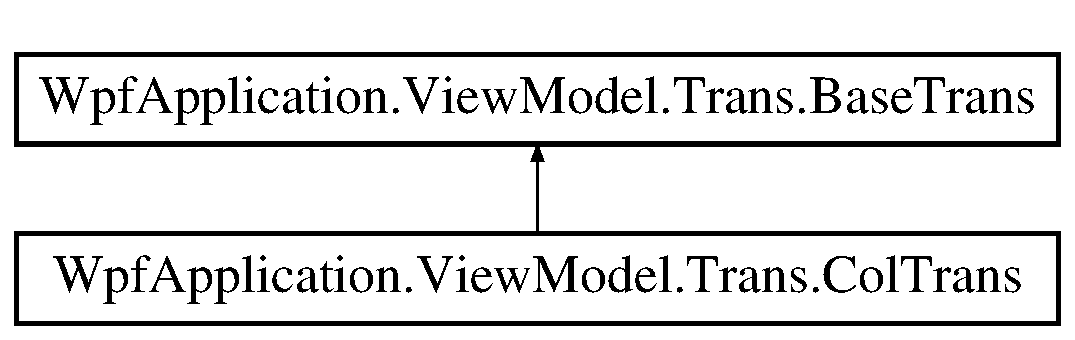
\includegraphics[height=2.000000cm]{class_wpf_application_1_1_view_model_1_1_trans_1_1_col_trans}
\end{center}
\end{figure}
\subsection*{Public Member Functions}
\begin{DoxyCompactItemize}
\item 
\hyperlink{class_wpf_application_1_1_view_model_1_1_trans_1_1_col_trans_a10806d4b09cb15edf1bdc68f650cc072}{Col\-Trans} (int mat, string \hyperlink{class_wpf_application_1_1_view_model_1_1_trans_1_1_col_trans_a4a0175ae91e92eff8ab56141df9d745d}{nom}, string \hyperlink{class_wpf_application_1_1_view_model_1_1_trans_1_1_col_trans_a3a74c60e37c799adda7bb94e1f8015b0}{prenom})
\item 
\hyperlink{class_wpf_application_1_1_view_model_1_1_trans_1_1_col_trans_af8b84e5512c2ac1764305e75a348be32}{Col\-Trans} (\hyperlink{class_wpf_application_1_1_view_model_1_1_trans_1_1_col_trans}{Col\-Trans} c)
\item 
override string \hyperlink{class_wpf_application_1_1_view_model_1_1_trans_1_1_col_trans_a07b2e23b8b3f221e6b5538d7666454e8}{To\-String} ()
\item 
string \hyperlink{class_wpf_application_1_1_view_model_1_1_trans_1_1_col_trans_a38ddd23b769263abad93935674851179}{To\-Csv\-Row} ()
\begin{DoxyCompactList}\small\item\em Retourne une representation de l'instance sous forme d'une string, ligne d'un fichier C\-S\-V. Format\-: \char`\"{}col1;col2;col2\textbackslash{}n\char`\"{} \end{DoxyCompactList}\item 
override string \hyperlink{class_wpf_application_1_1_view_model_1_1_trans_1_1_col_trans_aa3df7badaefa8f6adeb0de1147b649bc}{get\-Class} ()
\end{DoxyCompactItemize}
\subsection*{Properties}
\begin{DoxyCompactItemize}
\item 
int \hyperlink{class_wpf_application_1_1_view_model_1_1_trans_1_1_col_trans_a3fb492f9af2e8b2230ec81bf1ed225ee}{matricule}\hspace{0.3cm}{\ttfamily  \mbox{[}get, set\mbox{]}}
\item 
string \hyperlink{class_wpf_application_1_1_view_model_1_1_trans_1_1_col_trans_a4a0175ae91e92eff8ab56141df9d745d}{nom}\hspace{0.3cm}{\ttfamily  \mbox{[}get, set\mbox{]}}
\item 
string \hyperlink{class_wpf_application_1_1_view_model_1_1_trans_1_1_col_trans_a3a74c60e37c799adda7bb94e1f8015b0}{prenom}\hspace{0.3cm}{\ttfamily  \mbox{[}get, set\mbox{]}}
\end{DoxyCompactItemize}


\subsection{Constructor \& Destructor Documentation}
\hypertarget{class_wpf_application_1_1_view_model_1_1_trans_1_1_col_trans_a10806d4b09cb15edf1bdc68f650cc072}{\index{Wpf\-Application\-::\-View\-Model\-::\-Trans\-::\-Col\-Trans@{Wpf\-Application\-::\-View\-Model\-::\-Trans\-::\-Col\-Trans}!Col\-Trans@{Col\-Trans}}
\index{Col\-Trans@{Col\-Trans}!WpfApplication::ViewModel::Trans::ColTrans@{Wpf\-Application\-::\-View\-Model\-::\-Trans\-::\-Col\-Trans}}
\subsubsection[{Col\-Trans}]{\setlength{\rightskip}{0pt plus 5cm}Wpf\-Application.\-View\-Model.\-Trans.\-Col\-Trans.\-Col\-Trans (
\begin{DoxyParamCaption}
\item[{int}]{mat, }
\item[{string}]{nom, }
\item[{string}]{prenom}
\end{DoxyParamCaption}
)}}\label{class_wpf_application_1_1_view_model_1_1_trans_1_1_col_trans_a10806d4b09cb15edf1bdc68f650cc072}
\hypertarget{class_wpf_application_1_1_view_model_1_1_trans_1_1_col_trans_af8b84e5512c2ac1764305e75a348be32}{\index{Wpf\-Application\-::\-View\-Model\-::\-Trans\-::\-Col\-Trans@{Wpf\-Application\-::\-View\-Model\-::\-Trans\-::\-Col\-Trans}!Col\-Trans@{Col\-Trans}}
\index{Col\-Trans@{Col\-Trans}!WpfApplication::ViewModel::Trans::ColTrans@{Wpf\-Application\-::\-View\-Model\-::\-Trans\-::\-Col\-Trans}}
\subsubsection[{Col\-Trans}]{\setlength{\rightskip}{0pt plus 5cm}Wpf\-Application.\-View\-Model.\-Trans.\-Col\-Trans.\-Col\-Trans (
\begin{DoxyParamCaption}
\item[{{\bf Col\-Trans}}]{c}
\end{DoxyParamCaption}
)}}\label{class_wpf_application_1_1_view_model_1_1_trans_1_1_col_trans_af8b84e5512c2ac1764305e75a348be32}


\subsection{Member Function Documentation}
\hypertarget{class_wpf_application_1_1_view_model_1_1_trans_1_1_col_trans_aa3df7badaefa8f6adeb0de1147b649bc}{\index{Wpf\-Application\-::\-View\-Model\-::\-Trans\-::\-Col\-Trans@{Wpf\-Application\-::\-View\-Model\-::\-Trans\-::\-Col\-Trans}!get\-Class@{get\-Class}}
\index{get\-Class@{get\-Class}!WpfApplication::ViewModel::Trans::ColTrans@{Wpf\-Application\-::\-View\-Model\-::\-Trans\-::\-Col\-Trans}}
\subsubsection[{get\-Class}]{\setlength{\rightskip}{0pt plus 5cm}override string Wpf\-Application.\-View\-Model.\-Trans.\-Col\-Trans.\-get\-Class (
\begin{DoxyParamCaption}
{}
\end{DoxyParamCaption}
)\hspace{0.3cm}{\ttfamily [virtual]}}}\label{class_wpf_application_1_1_view_model_1_1_trans_1_1_col_trans_aa3df7badaefa8f6adeb0de1147b649bc}


Reimplemented from \hyperlink{class_wpf_application_1_1_view_model_1_1_trans_1_1_base_trans_a9660be8cb25ed5d666eab9ddd10600aa}{Wpf\-Application.\-View\-Model.\-Trans.\-Base\-Trans}.

\hypertarget{class_wpf_application_1_1_view_model_1_1_trans_1_1_col_trans_a38ddd23b769263abad93935674851179}{\index{Wpf\-Application\-::\-View\-Model\-::\-Trans\-::\-Col\-Trans@{Wpf\-Application\-::\-View\-Model\-::\-Trans\-::\-Col\-Trans}!To\-Csv\-Row@{To\-Csv\-Row}}
\index{To\-Csv\-Row@{To\-Csv\-Row}!WpfApplication::ViewModel::Trans::ColTrans@{Wpf\-Application\-::\-View\-Model\-::\-Trans\-::\-Col\-Trans}}
\subsubsection[{To\-Csv\-Row}]{\setlength{\rightskip}{0pt plus 5cm}string Wpf\-Application.\-View\-Model.\-Trans.\-Col\-Trans.\-To\-Csv\-Row (
\begin{DoxyParamCaption}
{}
\end{DoxyParamCaption}
)}}\label{class_wpf_application_1_1_view_model_1_1_trans_1_1_col_trans_a38ddd23b769263abad93935674851179}


Retourne une representation de l'instance sous forme d'une string, ligne d'un fichier C\-S\-V. Format\-: \char`\"{}col1;col2;col2\textbackslash{}n\char`\"{} 

\begin{DoxyReturn}{Returns}
String, separee par des ';' et terminee par '\par
'
\end{DoxyReturn}
\hypertarget{class_wpf_application_1_1_view_model_1_1_trans_1_1_col_trans_a07b2e23b8b3f221e6b5538d7666454e8}{\index{Wpf\-Application\-::\-View\-Model\-::\-Trans\-::\-Col\-Trans@{Wpf\-Application\-::\-View\-Model\-::\-Trans\-::\-Col\-Trans}!To\-String@{To\-String}}
\index{To\-String@{To\-String}!WpfApplication::ViewModel::Trans::ColTrans@{Wpf\-Application\-::\-View\-Model\-::\-Trans\-::\-Col\-Trans}}
\subsubsection[{To\-String}]{\setlength{\rightskip}{0pt plus 5cm}override string Wpf\-Application.\-View\-Model.\-Trans.\-Col\-Trans.\-To\-String (
\begin{DoxyParamCaption}
{}
\end{DoxyParamCaption}
)}}\label{class_wpf_application_1_1_view_model_1_1_trans_1_1_col_trans_a07b2e23b8b3f221e6b5538d7666454e8}


\subsection{Property Documentation}
\hypertarget{class_wpf_application_1_1_view_model_1_1_trans_1_1_col_trans_a3fb492f9af2e8b2230ec81bf1ed225ee}{\index{Wpf\-Application\-::\-View\-Model\-::\-Trans\-::\-Col\-Trans@{Wpf\-Application\-::\-View\-Model\-::\-Trans\-::\-Col\-Trans}!matricule@{matricule}}
\index{matricule@{matricule}!WpfApplication::ViewModel::Trans::ColTrans@{Wpf\-Application\-::\-View\-Model\-::\-Trans\-::\-Col\-Trans}}
\subsubsection[{matricule}]{\setlength{\rightskip}{0pt plus 5cm}int Wpf\-Application.\-View\-Model.\-Trans.\-Col\-Trans.\-matricule\hspace{0.3cm}{\ttfamily [get]}, {\ttfamily [set]}}}\label{class_wpf_application_1_1_view_model_1_1_trans_1_1_col_trans_a3fb492f9af2e8b2230ec81bf1ed225ee}
\hypertarget{class_wpf_application_1_1_view_model_1_1_trans_1_1_col_trans_a4a0175ae91e92eff8ab56141df9d745d}{\index{Wpf\-Application\-::\-View\-Model\-::\-Trans\-::\-Col\-Trans@{Wpf\-Application\-::\-View\-Model\-::\-Trans\-::\-Col\-Trans}!nom@{nom}}
\index{nom@{nom}!WpfApplication::ViewModel::Trans::ColTrans@{Wpf\-Application\-::\-View\-Model\-::\-Trans\-::\-Col\-Trans}}
\subsubsection[{nom}]{\setlength{\rightskip}{0pt plus 5cm}string Wpf\-Application.\-View\-Model.\-Trans.\-Col\-Trans.\-nom\hspace{0.3cm}{\ttfamily [get]}, {\ttfamily [set]}}}\label{class_wpf_application_1_1_view_model_1_1_trans_1_1_col_trans_a4a0175ae91e92eff8ab56141df9d745d}
\hypertarget{class_wpf_application_1_1_view_model_1_1_trans_1_1_col_trans_a3a74c60e37c799adda7bb94e1f8015b0}{\index{Wpf\-Application\-::\-View\-Model\-::\-Trans\-::\-Col\-Trans@{Wpf\-Application\-::\-View\-Model\-::\-Trans\-::\-Col\-Trans}!prenom@{prenom}}
\index{prenom@{prenom}!WpfApplication::ViewModel::Trans::ColTrans@{Wpf\-Application\-::\-View\-Model\-::\-Trans\-::\-Col\-Trans}}
\subsubsection[{prenom}]{\setlength{\rightskip}{0pt plus 5cm}string Wpf\-Application.\-View\-Model.\-Trans.\-Col\-Trans.\-prenom\hspace{0.3cm}{\ttfamily [get]}, {\ttfamily [set]}}}\label{class_wpf_application_1_1_view_model_1_1_trans_1_1_col_trans_a3a74c60e37c799adda7bb94e1f8015b0}


The documentation for this class was generated from the following file\-:\begin{DoxyCompactItemize}
\item 
C\-:/\-Users/dju/\-Documents/\-Visual Studio 2012/\-Projects/\-P\-P\-E/\-P\-P\-E3/\-Wpf\-Application/\-View\-Model/\-Trans/\hyperlink{_col_trans_8cs}{Col\-Trans.\-cs}\end{DoxyCompactItemize}

\hypertarget{class_model_1_1_c_o_m_m_u_n_e}{\section{Model.\-C\-O\-M\-M\-U\-N\-E Class Reference}
\label{class_model_1_1_c_o_m_m_u_n_e}\index{Model.\-C\-O\-M\-M\-U\-N\-E@{Model.\-C\-O\-M\-M\-U\-N\-E}}
}


Aucune documentation sur les métadonnées n'est disponible.  


Inheritance diagram for Model.\-C\-O\-M\-M\-U\-N\-E\-:\begin{figure}[H]
\begin{center}
\leavevmode
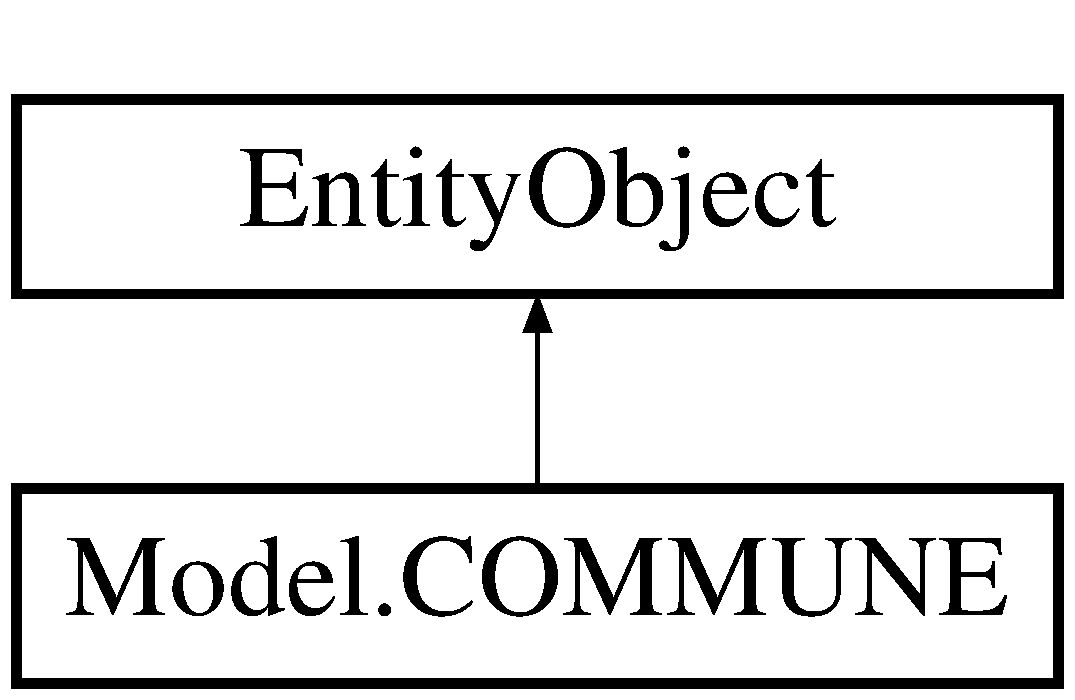
\includegraphics[height=2.000000cm]{class_model_1_1_c_o_m_m_u_n_e}
\end{center}
\end{figure}
\subsection*{Static Public Member Functions}
\begin{DoxyCompactItemize}
\item 
static \hyperlink{class_model_1_1_c_o_m_m_u_n_e}{C\-O\-M\-M\-U\-N\-E} \hyperlink{class_model_1_1_c_o_m_m_u_n_e_a4462879810e735f36043e31fa7ae4dda}{Create\-C\-O\-M\-M\-U\-N\-E} (global\-::\-System.\-String \hyperlink{class_model_1_1_c_o_m_m_u_n_e_aee3168256be0d999cdc2a6db66875cf9}{code\-\_\-commune}, global\-::\-System.\-String \hyperlink{class_model_1_1_c_o_m_m_u_n_e_a7e5b6345cd53c93bc68aadbf0846038d}{libelle\-\_\-commun})
\begin{DoxyCompactList}\small\item\em Créez un nouvel objet \hyperlink{class_model_1_1_c_o_m_m_u_n_e}{C\-O\-M\-M\-U\-N\-E}. \end{DoxyCompactList}\end{DoxyCompactItemize}
\subsection*{Properties}
\begin{DoxyCompactItemize}
\item 
global\-::\-System.\-String \hyperlink{class_model_1_1_c_o_m_m_u_n_e_aee3168256be0d999cdc2a6db66875cf9}{code\-\_\-commune}\hspace{0.3cm}{\ttfamily  \mbox{[}get, set\mbox{]}}
\begin{DoxyCompactList}\small\item\em Aucune documentation sur les métadonnées n'est disponible. \end{DoxyCompactList}\item 
global\-::\-System.\-String \hyperlink{class_model_1_1_c_o_m_m_u_n_e_a0c96be96f831dddcb05051cf3513986b}{code\-\_\-dep}\hspace{0.3cm}{\ttfamily  \mbox{[}get, set\mbox{]}}
\begin{DoxyCompactList}\small\item\em Aucune documentation sur les métadonnées n'est disponible. \end{DoxyCompactList}\item 
global\-::\-System.\-String \hyperlink{class_model_1_1_c_o_m_m_u_n_e_a7e5b6345cd53c93bc68aadbf0846038d}{libelle\-\_\-commun}\hspace{0.3cm}{\ttfamily  \mbox{[}get, set\mbox{]}}
\begin{DoxyCompactList}\small\item\em Aucune documentation sur les métadonnées n'est disponible. \end{DoxyCompactList}\item 
\hyperlink{class_model_1_1_d_e_p_a_r_t_e_m_e_n_t}{D\-E\-P\-A\-R\-T\-E\-M\-E\-N\-T} \hyperlink{class_model_1_1_c_o_m_m_u_n_e_a0b2beac6a64f8fa9413209ff4dae52f6}{D\-E\-P\-A\-R\-T\-E\-M\-E\-N\-T}\hspace{0.3cm}{\ttfamily  \mbox{[}get, set\mbox{]}}
\begin{DoxyCompactList}\small\item\em Aucune documentation sur les métadonnées n'est disponible. \end{DoxyCompactList}\item 
Entity\-Reference$<$ \hyperlink{class_model_1_1_d_e_p_a_r_t_e_m_e_n_t}{D\-E\-P\-A\-R\-T\-E\-M\-E\-N\-T} $>$ \hyperlink{class_model_1_1_c_o_m_m_u_n_e_a6561fcb5ec3bd228f22d5169b60ee1ba}{D\-E\-P\-A\-R\-T\-E\-M\-E\-N\-T\-Reference}\hspace{0.3cm}{\ttfamily  \mbox{[}get, set\mbox{]}}
\begin{DoxyCompactList}\small\item\em Aucune documentation sur les métadonnées n'est disponible. \end{DoxyCompactList}\end{DoxyCompactItemize}


\subsection{Detailed Description}
Aucune documentation sur les métadonnées n'est disponible. 



\subsection{Member Function Documentation}
\hypertarget{class_model_1_1_c_o_m_m_u_n_e_a4462879810e735f36043e31fa7ae4dda}{\index{Model\-::\-C\-O\-M\-M\-U\-N\-E@{Model\-::\-C\-O\-M\-M\-U\-N\-E}!Create\-C\-O\-M\-M\-U\-N\-E@{Create\-C\-O\-M\-M\-U\-N\-E}}
\index{Create\-C\-O\-M\-M\-U\-N\-E@{Create\-C\-O\-M\-M\-U\-N\-E}!Model::COMMUNE@{Model\-::\-C\-O\-M\-M\-U\-N\-E}}
\subsubsection[{Create\-C\-O\-M\-M\-U\-N\-E}]{\setlength{\rightskip}{0pt plus 5cm}static {\bf C\-O\-M\-M\-U\-N\-E} Model.\-C\-O\-M\-M\-U\-N\-E.\-Create\-C\-O\-M\-M\-U\-N\-E (
\begin{DoxyParamCaption}
\item[{global\-::\-System.\-String}]{code\-\_\-commune, }
\item[{global\-::\-System.\-String}]{libelle\-\_\-commun}
\end{DoxyParamCaption}
)\hspace{0.3cm}{\ttfamily [static]}}}\label{class_model_1_1_c_o_m_m_u_n_e_a4462879810e735f36043e31fa7ae4dda}


Créez un nouvel objet \hyperlink{class_model_1_1_c_o_m_m_u_n_e}{C\-O\-M\-M\-U\-N\-E}. 


\begin{DoxyParams}{Parameters}
{\em code\-\_\-commune} & Valeur initiale de la propriété code\-\_\-commune.\\
\hline
{\em libelle\-\_\-commun} & Valeur initiale de la propriété libelle\-\_\-commun.\\
\hline
\end{DoxyParams}


\subsection{Property Documentation}
\hypertarget{class_model_1_1_c_o_m_m_u_n_e_aee3168256be0d999cdc2a6db66875cf9}{\index{Model\-::\-C\-O\-M\-M\-U\-N\-E@{Model\-::\-C\-O\-M\-M\-U\-N\-E}!code\-\_\-commune@{code\-\_\-commune}}
\index{code\-\_\-commune@{code\-\_\-commune}!Model::COMMUNE@{Model\-::\-C\-O\-M\-M\-U\-N\-E}}
\subsubsection[{code\-\_\-commune}]{\setlength{\rightskip}{0pt plus 5cm}global.\-System.\-String Model.\-C\-O\-M\-M\-U\-N\-E.\-code\-\_\-commune\hspace{0.3cm}{\ttfamily [get]}, {\ttfamily [set]}}}\label{class_model_1_1_c_o_m_m_u_n_e_aee3168256be0d999cdc2a6db66875cf9}


Aucune documentation sur les métadonnées n'est disponible. 

\hypertarget{class_model_1_1_c_o_m_m_u_n_e_a0c96be96f831dddcb05051cf3513986b}{\index{Model\-::\-C\-O\-M\-M\-U\-N\-E@{Model\-::\-C\-O\-M\-M\-U\-N\-E}!code\-\_\-dep@{code\-\_\-dep}}
\index{code\-\_\-dep@{code\-\_\-dep}!Model::COMMUNE@{Model\-::\-C\-O\-M\-M\-U\-N\-E}}
\subsubsection[{code\-\_\-dep}]{\setlength{\rightskip}{0pt plus 5cm}global.\-System.\-String Model.\-C\-O\-M\-M\-U\-N\-E.\-code\-\_\-dep\hspace{0.3cm}{\ttfamily [get]}, {\ttfamily [set]}}}\label{class_model_1_1_c_o_m_m_u_n_e_a0c96be96f831dddcb05051cf3513986b}


Aucune documentation sur les métadonnées n'est disponible. 

\hypertarget{class_model_1_1_c_o_m_m_u_n_e_a0b2beac6a64f8fa9413209ff4dae52f6}{\index{Model\-::\-C\-O\-M\-M\-U\-N\-E@{Model\-::\-C\-O\-M\-M\-U\-N\-E}!D\-E\-P\-A\-R\-T\-E\-M\-E\-N\-T@{D\-E\-P\-A\-R\-T\-E\-M\-E\-N\-T}}
\index{D\-E\-P\-A\-R\-T\-E\-M\-E\-N\-T@{D\-E\-P\-A\-R\-T\-E\-M\-E\-N\-T}!Model::COMMUNE@{Model\-::\-C\-O\-M\-M\-U\-N\-E}}
\subsubsection[{D\-E\-P\-A\-R\-T\-E\-M\-E\-N\-T}]{\setlength{\rightskip}{0pt plus 5cm}{\bf D\-E\-P\-A\-R\-T\-E\-M\-E\-N\-T} Model.\-C\-O\-M\-M\-U\-N\-E.\-D\-E\-P\-A\-R\-T\-E\-M\-E\-N\-T\hspace{0.3cm}{\ttfamily [get]}, {\ttfamily [set]}}}\label{class_model_1_1_c_o_m_m_u_n_e_a0b2beac6a64f8fa9413209ff4dae52f6}


Aucune documentation sur les métadonnées n'est disponible. 

\hypertarget{class_model_1_1_c_o_m_m_u_n_e_a6561fcb5ec3bd228f22d5169b60ee1ba}{\index{Model\-::\-C\-O\-M\-M\-U\-N\-E@{Model\-::\-C\-O\-M\-M\-U\-N\-E}!D\-E\-P\-A\-R\-T\-E\-M\-E\-N\-T\-Reference@{D\-E\-P\-A\-R\-T\-E\-M\-E\-N\-T\-Reference}}
\index{D\-E\-P\-A\-R\-T\-E\-M\-E\-N\-T\-Reference@{D\-E\-P\-A\-R\-T\-E\-M\-E\-N\-T\-Reference}!Model::COMMUNE@{Model\-::\-C\-O\-M\-M\-U\-N\-E}}
\subsubsection[{D\-E\-P\-A\-R\-T\-E\-M\-E\-N\-T\-Reference}]{\setlength{\rightskip}{0pt plus 5cm}Entity\-Reference$<${\bf D\-E\-P\-A\-R\-T\-E\-M\-E\-N\-T}$>$ Model.\-C\-O\-M\-M\-U\-N\-E.\-D\-E\-P\-A\-R\-T\-E\-M\-E\-N\-T\-Reference\hspace{0.3cm}{\ttfamily [get]}, {\ttfamily [set]}}}\label{class_model_1_1_c_o_m_m_u_n_e_a6561fcb5ec3bd228f22d5169b60ee1ba}


Aucune documentation sur les métadonnées n'est disponible. 

\hypertarget{class_model_1_1_c_o_m_m_u_n_e_a7e5b6345cd53c93bc68aadbf0846038d}{\index{Model\-::\-C\-O\-M\-M\-U\-N\-E@{Model\-::\-C\-O\-M\-M\-U\-N\-E}!libelle\-\_\-commun@{libelle\-\_\-commun}}
\index{libelle\-\_\-commun@{libelle\-\_\-commun}!Model::COMMUNE@{Model\-::\-C\-O\-M\-M\-U\-N\-E}}
\subsubsection[{libelle\-\_\-commun}]{\setlength{\rightskip}{0pt plus 5cm}global.\-System.\-String Model.\-C\-O\-M\-M\-U\-N\-E.\-libelle\-\_\-commun\hspace{0.3cm}{\ttfamily [get]}, {\ttfamily [set]}}}\label{class_model_1_1_c_o_m_m_u_n_e_a7e5b6345cd53c93bc68aadbf0846038d}


Aucune documentation sur les métadonnées n'est disponible. 



The documentation for this class was generated from the following file\-:\begin{DoxyCompactItemize}
\item 
C\-:/\-Users/dju/\-Documents/\-Visual Studio 2012/\-Projects/\-P\-P\-E/\-P\-P\-E3/\-Model/\hyperlink{_model_bdd_sio_8_designer_8cs}{Model\-Bdd\-Sio.\-Designer.\-cs}\end{DoxyCompactItemize}

\hypertarget{class_model_1_1_c_o_m_p_o_s_a_n_t}{\section{Model.\-C\-O\-M\-P\-O\-S\-A\-N\-T Class Reference}
\label{class_model_1_1_c_o_m_p_o_s_a_n_t}\index{Model.\-C\-O\-M\-P\-O\-S\-A\-N\-T@{Model.\-C\-O\-M\-P\-O\-S\-A\-N\-T}}
}


Aucune documentation sur les métadonnées n'est disponible.  


Inheritance diagram for Model.\-C\-O\-M\-P\-O\-S\-A\-N\-T\-:\begin{figure}[H]
\begin{center}
\leavevmode
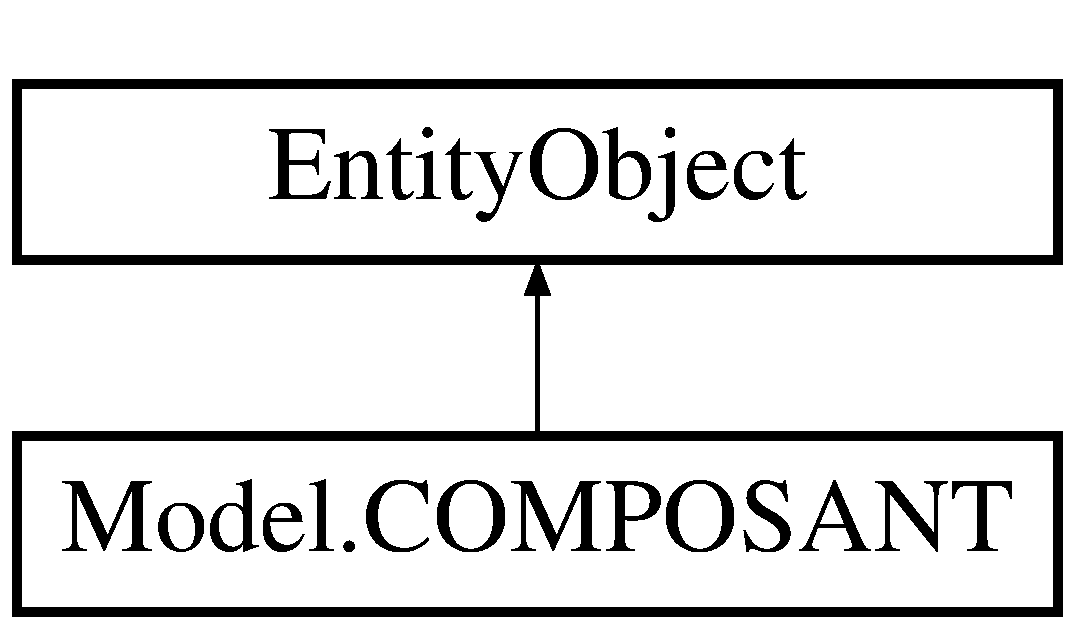
\includegraphics[height=2.000000cm]{class_model_1_1_c_o_m_p_o_s_a_n_t}
\end{center}
\end{figure}
\subsection*{Static Public Member Functions}
\begin{DoxyCompactItemize}
\item 
static \hyperlink{class_model_1_1_c_o_m_p_o_s_a_n_t}{C\-O\-M\-P\-O\-S\-A\-N\-T} \hyperlink{class_model_1_1_c_o_m_p_o_s_a_n_t_aad0d682b743b1d72a3ed03a373e07f72}{Create\-C\-O\-M\-P\-O\-S\-A\-N\-T} (global\-::\-System.\-Int32 \hyperlink{class_model_1_1_c_o_m_p_o_s_a_n_t_a29f8a5ee13f9d217125a207dcf378c2c}{code\-\_\-comp}, global\-::\-System.\-String \hyperlink{class_model_1_1_c_o_m_p_o_s_a_n_t_a238618dd950cff9c1d8cced54be482bb}{libelle\-\_\-comp})
\begin{DoxyCompactList}\small\item\em Créez un nouvel objet \hyperlink{class_model_1_1_c_o_m_p_o_s_a_n_t}{C\-O\-M\-P\-O\-S\-A\-N\-T}. \end{DoxyCompactList}\end{DoxyCompactItemize}
\subsection*{Properties}
\begin{DoxyCompactItemize}
\item 
global\-::\-System.\-Int32 \hyperlink{class_model_1_1_c_o_m_p_o_s_a_n_t_a29f8a5ee13f9d217125a207dcf378c2c}{code\-\_\-comp}\hspace{0.3cm}{\ttfamily  \mbox{[}get, set\mbox{]}}
\begin{DoxyCompactList}\small\item\em Aucune documentation sur les métadonnées n'est disponible. \end{DoxyCompactList}\item 
global\-::\-System.\-String \hyperlink{class_model_1_1_c_o_m_p_o_s_a_n_t_a238618dd950cff9c1d8cced54be482bb}{libelle\-\_\-comp}\hspace{0.3cm}{\ttfamily  \mbox{[}get, set\mbox{]}}
\begin{DoxyCompactList}\small\item\em Aucune documentation sur les métadonnées n'est disponible. \end{DoxyCompactList}\item 
Entity\-Collection$<$ \hyperlink{class_model_1_1_m_e_d_i_c_a_m_e_n_t}{M\-E\-D\-I\-C\-A\-M\-E\-N\-T} $>$ \hyperlink{class_model_1_1_c_o_m_p_o_s_a_n_t_a84bbd2e702acaac88ac584599f8f26a1}{M\-E\-D\-I\-C\-A\-M\-E\-N\-T}\hspace{0.3cm}{\ttfamily  \mbox{[}get, set\mbox{]}}
\begin{DoxyCompactList}\small\item\em Aucune documentation sur les métadonnées n'est disponible. \end{DoxyCompactList}\end{DoxyCompactItemize}


\subsection{Detailed Description}
Aucune documentation sur les métadonnées n'est disponible. 



\subsection{Member Function Documentation}
\hypertarget{class_model_1_1_c_o_m_p_o_s_a_n_t_aad0d682b743b1d72a3ed03a373e07f72}{\index{Model\-::\-C\-O\-M\-P\-O\-S\-A\-N\-T@{Model\-::\-C\-O\-M\-P\-O\-S\-A\-N\-T}!Create\-C\-O\-M\-P\-O\-S\-A\-N\-T@{Create\-C\-O\-M\-P\-O\-S\-A\-N\-T}}
\index{Create\-C\-O\-M\-P\-O\-S\-A\-N\-T@{Create\-C\-O\-M\-P\-O\-S\-A\-N\-T}!Model::COMPOSANT@{Model\-::\-C\-O\-M\-P\-O\-S\-A\-N\-T}}
\subsubsection[{Create\-C\-O\-M\-P\-O\-S\-A\-N\-T}]{\setlength{\rightskip}{0pt plus 5cm}static {\bf C\-O\-M\-P\-O\-S\-A\-N\-T} Model.\-C\-O\-M\-P\-O\-S\-A\-N\-T.\-Create\-C\-O\-M\-P\-O\-S\-A\-N\-T (
\begin{DoxyParamCaption}
\item[{global\-::\-System.\-Int32}]{code\-\_\-comp, }
\item[{global\-::\-System.\-String}]{libelle\-\_\-comp}
\end{DoxyParamCaption}
)\hspace{0.3cm}{\ttfamily [static]}}}\label{class_model_1_1_c_o_m_p_o_s_a_n_t_aad0d682b743b1d72a3ed03a373e07f72}


Créez un nouvel objet \hyperlink{class_model_1_1_c_o_m_p_o_s_a_n_t}{C\-O\-M\-P\-O\-S\-A\-N\-T}. 


\begin{DoxyParams}{Parameters}
{\em code\-\_\-comp} & Valeur initiale de la propriété code\-\_\-comp.\\
\hline
{\em libelle\-\_\-comp} & Valeur initiale de la propriété libelle\-\_\-comp.\\
\hline
\end{DoxyParams}


\subsection{Property Documentation}
\hypertarget{class_model_1_1_c_o_m_p_o_s_a_n_t_a29f8a5ee13f9d217125a207dcf378c2c}{\index{Model\-::\-C\-O\-M\-P\-O\-S\-A\-N\-T@{Model\-::\-C\-O\-M\-P\-O\-S\-A\-N\-T}!code\-\_\-comp@{code\-\_\-comp}}
\index{code\-\_\-comp@{code\-\_\-comp}!Model::COMPOSANT@{Model\-::\-C\-O\-M\-P\-O\-S\-A\-N\-T}}
\subsubsection[{code\-\_\-comp}]{\setlength{\rightskip}{0pt plus 5cm}global.\-System.\-Int32 Model.\-C\-O\-M\-P\-O\-S\-A\-N\-T.\-code\-\_\-comp\hspace{0.3cm}{\ttfamily [get]}, {\ttfamily [set]}}}\label{class_model_1_1_c_o_m_p_o_s_a_n_t_a29f8a5ee13f9d217125a207dcf378c2c}


Aucune documentation sur les métadonnées n'est disponible. 

\hypertarget{class_model_1_1_c_o_m_p_o_s_a_n_t_a238618dd950cff9c1d8cced54be482bb}{\index{Model\-::\-C\-O\-M\-P\-O\-S\-A\-N\-T@{Model\-::\-C\-O\-M\-P\-O\-S\-A\-N\-T}!libelle\-\_\-comp@{libelle\-\_\-comp}}
\index{libelle\-\_\-comp@{libelle\-\_\-comp}!Model::COMPOSANT@{Model\-::\-C\-O\-M\-P\-O\-S\-A\-N\-T}}
\subsubsection[{libelle\-\_\-comp}]{\setlength{\rightskip}{0pt plus 5cm}global.\-System.\-String Model.\-C\-O\-M\-P\-O\-S\-A\-N\-T.\-libelle\-\_\-comp\hspace{0.3cm}{\ttfamily [get]}, {\ttfamily [set]}}}\label{class_model_1_1_c_o_m_p_o_s_a_n_t_a238618dd950cff9c1d8cced54be482bb}


Aucune documentation sur les métadonnées n'est disponible. 

\hypertarget{class_model_1_1_c_o_m_p_o_s_a_n_t_a84bbd2e702acaac88ac584599f8f26a1}{\index{Model\-::\-C\-O\-M\-P\-O\-S\-A\-N\-T@{Model\-::\-C\-O\-M\-P\-O\-S\-A\-N\-T}!M\-E\-D\-I\-C\-A\-M\-E\-N\-T@{M\-E\-D\-I\-C\-A\-M\-E\-N\-T}}
\index{M\-E\-D\-I\-C\-A\-M\-E\-N\-T@{M\-E\-D\-I\-C\-A\-M\-E\-N\-T}!Model::COMPOSANT@{Model\-::\-C\-O\-M\-P\-O\-S\-A\-N\-T}}
\subsubsection[{M\-E\-D\-I\-C\-A\-M\-E\-N\-T}]{\setlength{\rightskip}{0pt plus 5cm}Entity\-Collection$<${\bf M\-E\-D\-I\-C\-A\-M\-E\-N\-T}$>$ Model.\-C\-O\-M\-P\-O\-S\-A\-N\-T.\-M\-E\-D\-I\-C\-A\-M\-E\-N\-T\hspace{0.3cm}{\ttfamily [get]}, {\ttfamily [set]}}}\label{class_model_1_1_c_o_m_p_o_s_a_n_t_a84bbd2e702acaac88ac584599f8f26a1}


Aucune documentation sur les métadonnées n'est disponible. 



The documentation for this class was generated from the following file\-:\begin{DoxyCompactItemize}
\item 
C\-:/\-Users/dju/\-Documents/\-Visual Studio 2012/\-Projects/\-P\-P\-E/\-P\-P\-E3/\-Model/\hyperlink{_model_bdd_sio_8_designer_8cs}{Model\-Bdd\-Sio.\-Designer.\-cs}\end{DoxyCompactItemize}

\hypertarget{class_model_1_1_d_a_t_e}{\section{Model.\-D\-A\-T\-E Class Reference}
\label{class_model_1_1_d_a_t_e}\index{Model.\-D\-A\-T\-E@{Model.\-D\-A\-T\-E}}
}


Aucune documentation sur les métadonnées n'est disponible.  


Inheritance diagram for Model.\-D\-A\-T\-E\-:\begin{figure}[H]
\begin{center}
\leavevmode
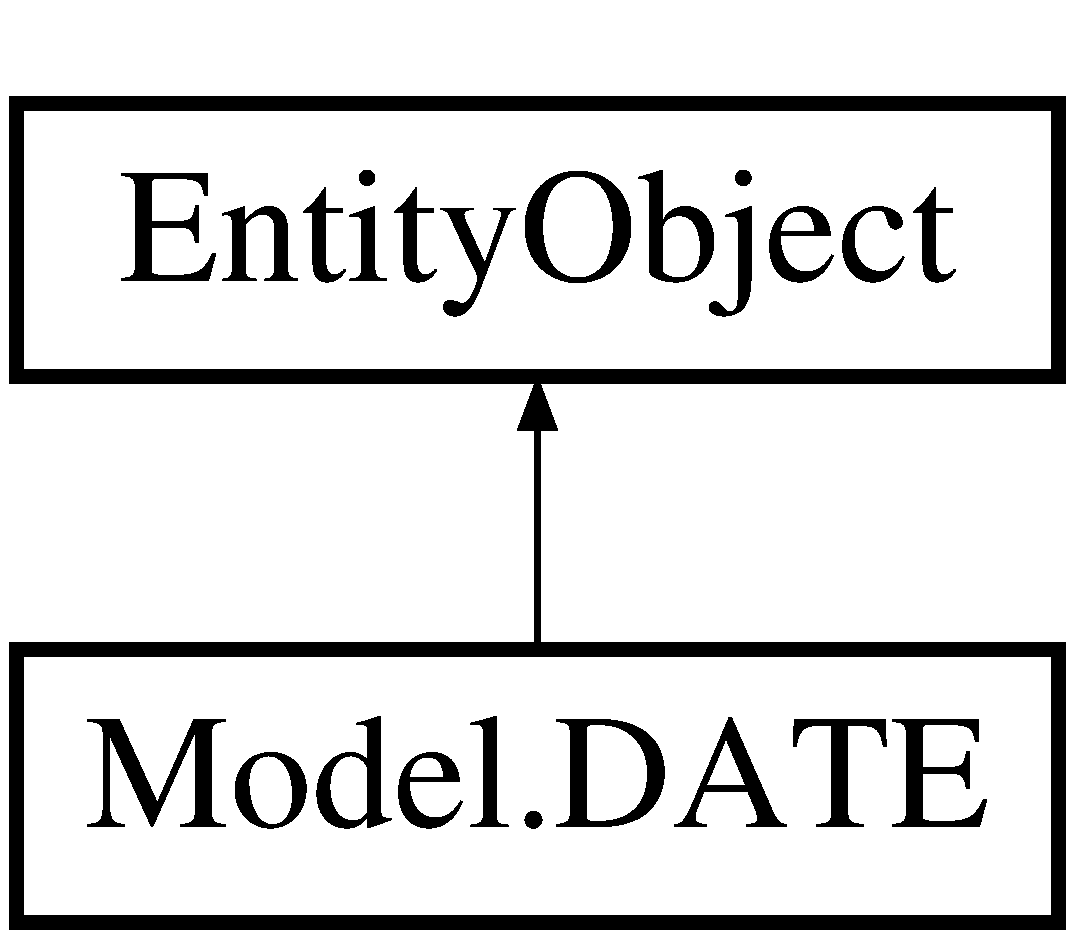
\includegraphics[height=2.000000cm]{class_model_1_1_d_a_t_e}
\end{center}
\end{figure}
\subsection*{Static Public Member Functions}
\begin{DoxyCompactItemize}
\item 
static \hyperlink{class_model_1_1_d_a_t_e}{D\-A\-T\-E} \hyperlink{class_model_1_1_d_a_t_e_ae765dee9b8e798c923cf5e7ae684be6c}{Create\-D\-A\-T\-E} (global\-::\-System.\-Date\-Time j\-J\-M\-M\-A\-A\-A\-A)
\begin{DoxyCompactList}\small\item\em Créez un nouvel objet \hyperlink{class_model_1_1_d_a_t_e}{D\-A\-T\-E}. \end{DoxyCompactList}\end{DoxyCompactItemize}
\subsection*{Properties}
\begin{DoxyCompactItemize}
\item 
global\-::\-System.\-Date\-Time \hyperlink{class_model_1_1_d_a_t_e_a235454d739b3af26e48977c29d385907}{J\-J\-M\-M\-A\-A\-A\-A}\hspace{0.3cm}{\ttfamily  \mbox{[}get, set\mbox{]}}
\begin{DoxyCompactList}\small\item\em Aucune documentation sur les métadonnées n'est disponible. \end{DoxyCompactList}\item 
Entity\-Collection$<$ \hyperlink{class_model_1_1_r_e_m_p_l_a_c_e}{R\-E\-M\-P\-L\-A\-C\-E} $>$ \hyperlink{class_model_1_1_d_a_t_e_ab660780ffb5bef16c7c3632f69eaa926}{R\-E\-M\-P\-L\-A\-C\-E}\hspace{0.3cm}{\ttfamily  \mbox{[}get, set\mbox{]}}
\begin{DoxyCompactList}\small\item\em Aucune documentation sur les métadonnées n'est disponible. \end{DoxyCompactList}\end{DoxyCompactItemize}


\subsection{Detailed Description}
Aucune documentation sur les métadonnées n'est disponible. 



\subsection{Member Function Documentation}
\hypertarget{class_model_1_1_d_a_t_e_ae765dee9b8e798c923cf5e7ae684be6c}{\index{Model\-::\-D\-A\-T\-E@{Model\-::\-D\-A\-T\-E}!Create\-D\-A\-T\-E@{Create\-D\-A\-T\-E}}
\index{Create\-D\-A\-T\-E@{Create\-D\-A\-T\-E}!Model::DATE@{Model\-::\-D\-A\-T\-E}}
\subsubsection[{Create\-D\-A\-T\-E}]{\setlength{\rightskip}{0pt plus 5cm}static {\bf D\-A\-T\-E} Model.\-D\-A\-T\-E.\-Create\-D\-A\-T\-E (
\begin{DoxyParamCaption}
\item[{global\-::\-System.\-Date\-Time}]{j\-J\-M\-M\-A\-A\-A\-A}
\end{DoxyParamCaption}
)\hspace{0.3cm}{\ttfamily [static]}}}\label{class_model_1_1_d_a_t_e_ae765dee9b8e798c923cf5e7ae684be6c}


Créez un nouvel objet \hyperlink{class_model_1_1_d_a_t_e}{D\-A\-T\-E}. 


\begin{DoxyParams}{Parameters}
{\em j\-J\-M\-M\-A\-A\-A\-A} & Valeur initiale de la propriété J\-J\-M\-M\-A\-A\-A\-A.\\
\hline
\end{DoxyParams}


\subsection{Property Documentation}
\hypertarget{class_model_1_1_d_a_t_e_a235454d739b3af26e48977c29d385907}{\index{Model\-::\-D\-A\-T\-E@{Model\-::\-D\-A\-T\-E}!J\-J\-M\-M\-A\-A\-A\-A@{J\-J\-M\-M\-A\-A\-A\-A}}
\index{J\-J\-M\-M\-A\-A\-A\-A@{J\-J\-M\-M\-A\-A\-A\-A}!Model::DATE@{Model\-::\-D\-A\-T\-E}}
\subsubsection[{J\-J\-M\-M\-A\-A\-A\-A}]{\setlength{\rightskip}{0pt plus 5cm}global.\-System.\-Date\-Time Model.\-D\-A\-T\-E.\-J\-J\-M\-M\-A\-A\-A\-A\hspace{0.3cm}{\ttfamily [get]}, {\ttfamily [set]}}}\label{class_model_1_1_d_a_t_e_a235454d739b3af26e48977c29d385907}


Aucune documentation sur les métadonnées n'est disponible. 

\hypertarget{class_model_1_1_d_a_t_e_ab660780ffb5bef16c7c3632f69eaa926}{\index{Model\-::\-D\-A\-T\-E@{Model\-::\-D\-A\-T\-E}!R\-E\-M\-P\-L\-A\-C\-E@{R\-E\-M\-P\-L\-A\-C\-E}}
\index{R\-E\-M\-P\-L\-A\-C\-E@{R\-E\-M\-P\-L\-A\-C\-E}!Model::DATE@{Model\-::\-D\-A\-T\-E}}
\subsubsection[{R\-E\-M\-P\-L\-A\-C\-E}]{\setlength{\rightskip}{0pt plus 5cm}Entity\-Collection$<${\bf R\-E\-M\-P\-L\-A\-C\-E}$>$ Model.\-D\-A\-T\-E.\-R\-E\-M\-P\-L\-A\-C\-E\hspace{0.3cm}{\ttfamily [get]}, {\ttfamily [set]}}}\label{class_model_1_1_d_a_t_e_ab660780ffb5bef16c7c3632f69eaa926}


Aucune documentation sur les métadonnées n'est disponible. 



The documentation for this class was generated from the following file\-:\begin{DoxyCompactItemize}
\item 
C\-:/\-Users/dju/\-Documents/\-Visual Studio 2012/\-Projects/\-P\-P\-E/\-P\-P\-E3/\-Model/\hyperlink{_model_bdd_sio_8_designer_8cs}{Model\-Bdd\-Sio.\-Designer.\-cs}\end{DoxyCompactItemize}

\hypertarget{class_wpf_application_1_1_helpers_1_1_delegate_command}{\section{Wpf\-Application.\-Helpers.\-Delegate\-Command Class Reference}
\label{class_wpf_application_1_1_helpers_1_1_delegate_command}\index{Wpf\-Application.\-Helpers.\-Delegate\-Command@{Wpf\-Application.\-Helpers.\-Delegate\-Command}}
}
Inheritance diagram for Wpf\-Application.\-Helpers.\-Delegate\-Command\-:\begin{figure}[H]
\begin{center}
\leavevmode
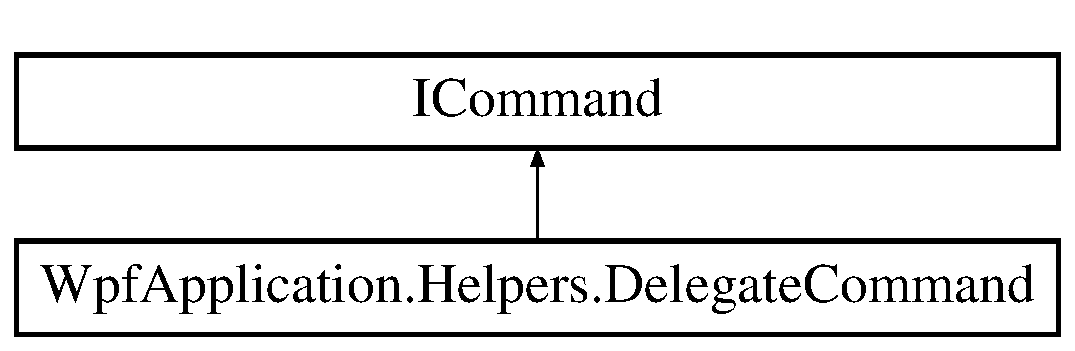
\includegraphics[height=2.000000cm]{class_wpf_application_1_1_helpers_1_1_delegate_command}
\end{center}
\end{figure}
\subsection*{Public Member Functions}
\begin{DoxyCompactItemize}
\item 
\hyperlink{class_wpf_application_1_1_helpers_1_1_delegate_command_a6bc65ddb546224275a5f98d46278b56f}{Delegate\-Command} (Action command, Func$<$ bool $>$ can\-Execute=null)
\item 
void \hyperlink{class_wpf_application_1_1_helpers_1_1_delegate_command_a21e894740c01f98e25f9d9fdda5b0d85}{Execute} (object parameter)
\item 
bool \hyperlink{class_wpf_application_1_1_helpers_1_1_delegate_command_a5be82ff4595bb5e13e4548b23d901de6}{Can\-Execute} (object parameter)
\end{DoxyCompactItemize}
\subsection*{Properties}
\begin{DoxyCompactItemize}
\item 
Event\-Handler \hyperlink{class_wpf_application_1_1_helpers_1_1_delegate_command_a92965ba61d3d0544387b3fcd6375e625}{Can\-Execute\-Changed}
\end{DoxyCompactItemize}


\subsection{Constructor \& Destructor Documentation}
\hypertarget{class_wpf_application_1_1_helpers_1_1_delegate_command_a6bc65ddb546224275a5f98d46278b56f}{\index{Wpf\-Application\-::\-Helpers\-::\-Delegate\-Command@{Wpf\-Application\-::\-Helpers\-::\-Delegate\-Command}!Delegate\-Command@{Delegate\-Command}}
\index{Delegate\-Command@{Delegate\-Command}!WpfApplication::Helpers::DelegateCommand@{Wpf\-Application\-::\-Helpers\-::\-Delegate\-Command}}
\subsubsection[{Delegate\-Command}]{\setlength{\rightskip}{0pt plus 5cm}Wpf\-Application.\-Helpers.\-Delegate\-Command.\-Delegate\-Command (
\begin{DoxyParamCaption}
\item[{Action}]{command, }
\item[{Func$<$ bool $>$}]{can\-Execute = {\ttfamily null}}
\end{DoxyParamCaption}
)}}\label{class_wpf_application_1_1_helpers_1_1_delegate_command_a6bc65ddb546224275a5f98d46278b56f}


\subsection{Member Function Documentation}
\hypertarget{class_wpf_application_1_1_helpers_1_1_delegate_command_a5be82ff4595bb5e13e4548b23d901de6}{\index{Wpf\-Application\-::\-Helpers\-::\-Delegate\-Command@{Wpf\-Application\-::\-Helpers\-::\-Delegate\-Command}!Can\-Execute@{Can\-Execute}}
\index{Can\-Execute@{Can\-Execute}!WpfApplication::Helpers::DelegateCommand@{Wpf\-Application\-::\-Helpers\-::\-Delegate\-Command}}
\subsubsection[{Can\-Execute}]{\setlength{\rightskip}{0pt plus 5cm}bool Wpf\-Application.\-Helpers.\-Delegate\-Command.\-Can\-Execute (
\begin{DoxyParamCaption}
\item[{object}]{parameter}
\end{DoxyParamCaption}
)}}\label{class_wpf_application_1_1_helpers_1_1_delegate_command_a5be82ff4595bb5e13e4548b23d901de6}
\hypertarget{class_wpf_application_1_1_helpers_1_1_delegate_command_a21e894740c01f98e25f9d9fdda5b0d85}{\index{Wpf\-Application\-::\-Helpers\-::\-Delegate\-Command@{Wpf\-Application\-::\-Helpers\-::\-Delegate\-Command}!Execute@{Execute}}
\index{Execute@{Execute}!WpfApplication::Helpers::DelegateCommand@{Wpf\-Application\-::\-Helpers\-::\-Delegate\-Command}}
\subsubsection[{Execute}]{\setlength{\rightskip}{0pt plus 5cm}void Wpf\-Application.\-Helpers.\-Delegate\-Command.\-Execute (
\begin{DoxyParamCaption}
\item[{object}]{parameter}
\end{DoxyParamCaption}
)}}\label{class_wpf_application_1_1_helpers_1_1_delegate_command_a21e894740c01f98e25f9d9fdda5b0d85}


\subsection{Property Documentation}
\hypertarget{class_wpf_application_1_1_helpers_1_1_delegate_command_a92965ba61d3d0544387b3fcd6375e625}{\index{Wpf\-Application\-::\-Helpers\-::\-Delegate\-Command@{Wpf\-Application\-::\-Helpers\-::\-Delegate\-Command}!Can\-Execute\-Changed@{Can\-Execute\-Changed}}
\index{Can\-Execute\-Changed@{Can\-Execute\-Changed}!WpfApplication::Helpers::DelegateCommand@{Wpf\-Application\-::\-Helpers\-::\-Delegate\-Command}}
\subsubsection[{Can\-Execute\-Changed}]{\setlength{\rightskip}{0pt plus 5cm}Event\-Handler Wpf\-Application.\-Helpers.\-Delegate\-Command.\-Can\-Execute\-Changed\hspace{0.3cm}{\ttfamily [add]}, {\ttfamily [remove]}}}\label{class_wpf_application_1_1_helpers_1_1_delegate_command_a92965ba61d3d0544387b3fcd6375e625}


The documentation for this class was generated from the following file\-:\begin{DoxyCompactItemize}
\item 
C\-:/\-Users/dju/\-Documents/\-Visual Studio 2012/\-Projects/\-P\-P\-E/\-P\-P\-E3/\-Wpf\-Application/\-Helpers/\hyperlink{_delegate_command_8cs}{Delegate\-Command.\-cs}\end{DoxyCompactItemize}

\hypertarget{class_model_1_1_d_e_p_a_r_t_e_m_e_n_t}{\section{Model.\-D\-E\-P\-A\-R\-T\-E\-M\-E\-N\-T Class Reference}
\label{class_model_1_1_d_e_p_a_r_t_e_m_e_n_t}\index{Model.\-D\-E\-P\-A\-R\-T\-E\-M\-E\-N\-T@{Model.\-D\-E\-P\-A\-R\-T\-E\-M\-E\-N\-T}}
}


Aucune documentation sur les métadonnées n'est disponible.  


Inheritance diagram for Model.\-D\-E\-P\-A\-R\-T\-E\-M\-E\-N\-T\-:\begin{figure}[H]
\begin{center}
\leavevmode
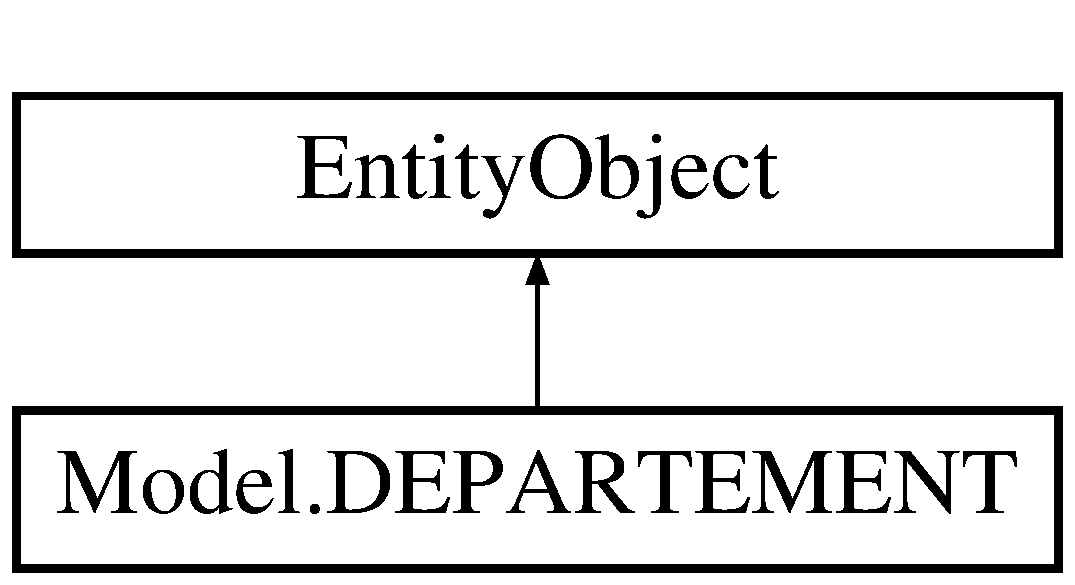
\includegraphics[height=2.000000cm]{class_model_1_1_d_e_p_a_r_t_e_m_e_n_t}
\end{center}
\end{figure}
\subsection*{Static Public Member Functions}
\begin{DoxyCompactItemize}
\item 
static \hyperlink{class_model_1_1_d_e_p_a_r_t_e_m_e_n_t}{D\-E\-P\-A\-R\-T\-E\-M\-E\-N\-T} \hyperlink{class_model_1_1_d_e_p_a_r_t_e_m_e_n_t_ac962c3ed325dec487f12f148711dccea}{Create\-D\-E\-P\-A\-R\-T\-E\-M\-E\-N\-T} (global\-::\-System.\-String \hyperlink{class_model_1_1_d_e_p_a_r_t_e_m_e_n_t_a2f34735310ea76c3f5b6cf158b85c314}{code\-\_\-dep}, global\-::\-System.\-String \hyperlink{class_model_1_1_d_e_p_a_r_t_e_m_e_n_t_aa1736783b4b382723941604c85f83a3f}{libelle\-\_\-dep})
\begin{DoxyCompactList}\small\item\em Créez un nouvel objet \hyperlink{class_model_1_1_d_e_p_a_r_t_e_m_e_n_t}{D\-E\-P\-A\-R\-T\-E\-M\-E\-N\-T}. \end{DoxyCompactList}\end{DoxyCompactItemize}
\subsection*{Properties}
\begin{DoxyCompactItemize}
\item 
global\-::\-System.\-String \hyperlink{class_model_1_1_d_e_p_a_r_t_e_m_e_n_t_a2f34735310ea76c3f5b6cf158b85c314}{code\-\_\-dep}\hspace{0.3cm}{\ttfamily  \mbox{[}get, set\mbox{]}}
\begin{DoxyCompactList}\small\item\em Aucune documentation sur les métadonnées n'est disponible. \end{DoxyCompactList}\item 
global\-::\-System.\-String \hyperlink{class_model_1_1_d_e_p_a_r_t_e_m_e_n_t_ab0e3826fb790a948c808c7ecabd4e2f9}{code\-\_\-region}\hspace{0.3cm}{\ttfamily  \mbox{[}get, set\mbox{]}}
\begin{DoxyCompactList}\small\item\em Aucune documentation sur les métadonnées n'est disponible. \end{DoxyCompactList}\item 
global\-::\-System.\-String \hyperlink{class_model_1_1_d_e_p_a_r_t_e_m_e_n_t_aa1736783b4b382723941604c85f83a3f}{libelle\-\_\-dep}\hspace{0.3cm}{\ttfamily  \mbox{[}get, set\mbox{]}}
\begin{DoxyCompactList}\small\item\em Aucune documentation sur les métadonnées n'est disponible. \end{DoxyCompactList}\item 
Entity\-Collection$<$ \hyperlink{class_model_1_1_c_o_m_m_u_n_e}{C\-O\-M\-M\-U\-N\-E} $>$ \hyperlink{class_model_1_1_d_e_p_a_r_t_e_m_e_n_t_a358ff1c2c8c59dcde2585fe932beac03}{C\-O\-M\-M\-U\-N\-E}\hspace{0.3cm}{\ttfamily  \mbox{[}get, set\mbox{]}}
\begin{DoxyCompactList}\small\item\em Aucune documentation sur les métadonnées n'est disponible. \end{DoxyCompactList}\item 
\hyperlink{class_model_1_1_r_e_g_i_o_n}{R\-E\-G\-I\-O\-N} \hyperlink{class_model_1_1_d_e_p_a_r_t_e_m_e_n_t_ab192797eea7cee21e42260494cce825a}{R\-E\-G\-I\-O\-N}\hspace{0.3cm}{\ttfamily  \mbox{[}get, set\mbox{]}}
\begin{DoxyCompactList}\small\item\em Aucune documentation sur les métadonnées n'est disponible. \end{DoxyCompactList}\item 
Entity\-Reference$<$ \hyperlink{class_model_1_1_r_e_g_i_o_n}{R\-E\-G\-I\-O\-N} $>$ \hyperlink{class_model_1_1_d_e_p_a_r_t_e_m_e_n_t_a55dd7dbfe43d8c3a15f0a0bef1d2ba20}{R\-E\-G\-I\-O\-N\-Reference}\hspace{0.3cm}{\ttfamily  \mbox{[}get, set\mbox{]}}
\begin{DoxyCompactList}\small\item\em Aucune documentation sur les métadonnées n'est disponible. \end{DoxyCompactList}\end{DoxyCompactItemize}


\subsection{Detailed Description}
Aucune documentation sur les métadonnées n'est disponible. 



\subsection{Member Function Documentation}
\hypertarget{class_model_1_1_d_e_p_a_r_t_e_m_e_n_t_ac962c3ed325dec487f12f148711dccea}{\index{Model\-::\-D\-E\-P\-A\-R\-T\-E\-M\-E\-N\-T@{Model\-::\-D\-E\-P\-A\-R\-T\-E\-M\-E\-N\-T}!Create\-D\-E\-P\-A\-R\-T\-E\-M\-E\-N\-T@{Create\-D\-E\-P\-A\-R\-T\-E\-M\-E\-N\-T}}
\index{Create\-D\-E\-P\-A\-R\-T\-E\-M\-E\-N\-T@{Create\-D\-E\-P\-A\-R\-T\-E\-M\-E\-N\-T}!Model::DEPARTEMENT@{Model\-::\-D\-E\-P\-A\-R\-T\-E\-M\-E\-N\-T}}
\subsubsection[{Create\-D\-E\-P\-A\-R\-T\-E\-M\-E\-N\-T}]{\setlength{\rightskip}{0pt plus 5cm}static {\bf D\-E\-P\-A\-R\-T\-E\-M\-E\-N\-T} Model.\-D\-E\-P\-A\-R\-T\-E\-M\-E\-N\-T.\-Create\-D\-E\-P\-A\-R\-T\-E\-M\-E\-N\-T (
\begin{DoxyParamCaption}
\item[{global\-::\-System.\-String}]{code\-\_\-dep, }
\item[{global\-::\-System.\-String}]{libelle\-\_\-dep}
\end{DoxyParamCaption}
)\hspace{0.3cm}{\ttfamily [static]}}}\label{class_model_1_1_d_e_p_a_r_t_e_m_e_n_t_ac962c3ed325dec487f12f148711dccea}


Créez un nouvel objet \hyperlink{class_model_1_1_d_e_p_a_r_t_e_m_e_n_t}{D\-E\-P\-A\-R\-T\-E\-M\-E\-N\-T}. 


\begin{DoxyParams}{Parameters}
{\em code\-\_\-dep} & Valeur initiale de la propriété code\-\_\-dep.\\
\hline
{\em libelle\-\_\-dep} & Valeur initiale de la propriété libelle\-\_\-dep.\\
\hline
\end{DoxyParams}


\subsection{Property Documentation}
\hypertarget{class_model_1_1_d_e_p_a_r_t_e_m_e_n_t_a2f34735310ea76c3f5b6cf158b85c314}{\index{Model\-::\-D\-E\-P\-A\-R\-T\-E\-M\-E\-N\-T@{Model\-::\-D\-E\-P\-A\-R\-T\-E\-M\-E\-N\-T}!code\-\_\-dep@{code\-\_\-dep}}
\index{code\-\_\-dep@{code\-\_\-dep}!Model::DEPARTEMENT@{Model\-::\-D\-E\-P\-A\-R\-T\-E\-M\-E\-N\-T}}
\subsubsection[{code\-\_\-dep}]{\setlength{\rightskip}{0pt plus 5cm}global.\-System.\-String Model.\-D\-E\-P\-A\-R\-T\-E\-M\-E\-N\-T.\-code\-\_\-dep\hspace{0.3cm}{\ttfamily [get]}, {\ttfamily [set]}}}\label{class_model_1_1_d_e_p_a_r_t_e_m_e_n_t_a2f34735310ea76c3f5b6cf158b85c314}


Aucune documentation sur les métadonnées n'est disponible. 

\hypertarget{class_model_1_1_d_e_p_a_r_t_e_m_e_n_t_ab0e3826fb790a948c808c7ecabd4e2f9}{\index{Model\-::\-D\-E\-P\-A\-R\-T\-E\-M\-E\-N\-T@{Model\-::\-D\-E\-P\-A\-R\-T\-E\-M\-E\-N\-T}!code\-\_\-region@{code\-\_\-region}}
\index{code\-\_\-region@{code\-\_\-region}!Model::DEPARTEMENT@{Model\-::\-D\-E\-P\-A\-R\-T\-E\-M\-E\-N\-T}}
\subsubsection[{code\-\_\-region}]{\setlength{\rightskip}{0pt plus 5cm}global.\-System.\-String Model.\-D\-E\-P\-A\-R\-T\-E\-M\-E\-N\-T.\-code\-\_\-region\hspace{0.3cm}{\ttfamily [get]}, {\ttfamily [set]}}}\label{class_model_1_1_d_e_p_a_r_t_e_m_e_n_t_ab0e3826fb790a948c808c7ecabd4e2f9}


Aucune documentation sur les métadonnées n'est disponible. 

\hypertarget{class_model_1_1_d_e_p_a_r_t_e_m_e_n_t_a358ff1c2c8c59dcde2585fe932beac03}{\index{Model\-::\-D\-E\-P\-A\-R\-T\-E\-M\-E\-N\-T@{Model\-::\-D\-E\-P\-A\-R\-T\-E\-M\-E\-N\-T}!C\-O\-M\-M\-U\-N\-E@{C\-O\-M\-M\-U\-N\-E}}
\index{C\-O\-M\-M\-U\-N\-E@{C\-O\-M\-M\-U\-N\-E}!Model::DEPARTEMENT@{Model\-::\-D\-E\-P\-A\-R\-T\-E\-M\-E\-N\-T}}
\subsubsection[{C\-O\-M\-M\-U\-N\-E}]{\setlength{\rightskip}{0pt plus 5cm}Entity\-Collection$<${\bf C\-O\-M\-M\-U\-N\-E}$>$ Model.\-D\-E\-P\-A\-R\-T\-E\-M\-E\-N\-T.\-C\-O\-M\-M\-U\-N\-E\hspace{0.3cm}{\ttfamily [get]}, {\ttfamily [set]}}}\label{class_model_1_1_d_e_p_a_r_t_e_m_e_n_t_a358ff1c2c8c59dcde2585fe932beac03}


Aucune documentation sur les métadonnées n'est disponible. 

\hypertarget{class_model_1_1_d_e_p_a_r_t_e_m_e_n_t_aa1736783b4b382723941604c85f83a3f}{\index{Model\-::\-D\-E\-P\-A\-R\-T\-E\-M\-E\-N\-T@{Model\-::\-D\-E\-P\-A\-R\-T\-E\-M\-E\-N\-T}!libelle\-\_\-dep@{libelle\-\_\-dep}}
\index{libelle\-\_\-dep@{libelle\-\_\-dep}!Model::DEPARTEMENT@{Model\-::\-D\-E\-P\-A\-R\-T\-E\-M\-E\-N\-T}}
\subsubsection[{libelle\-\_\-dep}]{\setlength{\rightskip}{0pt plus 5cm}global.\-System.\-String Model.\-D\-E\-P\-A\-R\-T\-E\-M\-E\-N\-T.\-libelle\-\_\-dep\hspace{0.3cm}{\ttfamily [get]}, {\ttfamily [set]}}}\label{class_model_1_1_d_e_p_a_r_t_e_m_e_n_t_aa1736783b4b382723941604c85f83a3f}


Aucune documentation sur les métadonnées n'est disponible. 

\hypertarget{class_model_1_1_d_e_p_a_r_t_e_m_e_n_t_ab192797eea7cee21e42260494cce825a}{\index{Model\-::\-D\-E\-P\-A\-R\-T\-E\-M\-E\-N\-T@{Model\-::\-D\-E\-P\-A\-R\-T\-E\-M\-E\-N\-T}!R\-E\-G\-I\-O\-N@{R\-E\-G\-I\-O\-N}}
\index{R\-E\-G\-I\-O\-N@{R\-E\-G\-I\-O\-N}!Model::DEPARTEMENT@{Model\-::\-D\-E\-P\-A\-R\-T\-E\-M\-E\-N\-T}}
\subsubsection[{R\-E\-G\-I\-O\-N}]{\setlength{\rightskip}{0pt plus 5cm}{\bf R\-E\-G\-I\-O\-N} Model.\-D\-E\-P\-A\-R\-T\-E\-M\-E\-N\-T.\-R\-E\-G\-I\-O\-N\hspace{0.3cm}{\ttfamily [get]}, {\ttfamily [set]}}}\label{class_model_1_1_d_e_p_a_r_t_e_m_e_n_t_ab192797eea7cee21e42260494cce825a}


Aucune documentation sur les métadonnées n'est disponible. 

\hypertarget{class_model_1_1_d_e_p_a_r_t_e_m_e_n_t_a55dd7dbfe43d8c3a15f0a0bef1d2ba20}{\index{Model\-::\-D\-E\-P\-A\-R\-T\-E\-M\-E\-N\-T@{Model\-::\-D\-E\-P\-A\-R\-T\-E\-M\-E\-N\-T}!R\-E\-G\-I\-O\-N\-Reference@{R\-E\-G\-I\-O\-N\-Reference}}
\index{R\-E\-G\-I\-O\-N\-Reference@{R\-E\-G\-I\-O\-N\-Reference}!Model::DEPARTEMENT@{Model\-::\-D\-E\-P\-A\-R\-T\-E\-M\-E\-N\-T}}
\subsubsection[{R\-E\-G\-I\-O\-N\-Reference}]{\setlength{\rightskip}{0pt plus 5cm}Entity\-Reference$<${\bf R\-E\-G\-I\-O\-N}$>$ Model.\-D\-E\-P\-A\-R\-T\-E\-M\-E\-N\-T.\-R\-E\-G\-I\-O\-N\-Reference\hspace{0.3cm}{\ttfamily [get]}, {\ttfamily [set]}}}\label{class_model_1_1_d_e_p_a_r_t_e_m_e_n_t_a55dd7dbfe43d8c3a15f0a0bef1d2ba20}


Aucune documentation sur les métadonnées n'est disponible. 



The documentation for this class was generated from the following file\-:\begin{DoxyCompactItemize}
\item 
C\-:/\-Users/dju/\-Documents/\-Visual Studio 2012/\-Projects/\-P\-P\-E/\-P\-P\-E3/\-Model/\hyperlink{_model_bdd_sio_8_designer_8cs}{Model\-Bdd\-Sio.\-Designer.\-cs}\end{DoxyCompactItemize}

\hypertarget{class_wpf_application_1_1_model_1_1_design_1_1_design_service_client}{\section{Wpf\-Application.\-Model.\-Design.\-Design\-Service\-Client Class Reference}
\label{class_wpf_application_1_1_model_1_1_design_1_1_design_service_client}\index{Wpf\-Application.\-Model.\-Design.\-Design\-Service\-Client@{Wpf\-Application.\-Model.\-Design.\-Design\-Service\-Client}}
}
Inheritance diagram for Wpf\-Application.\-Model.\-Design.\-Design\-Service\-Client\-:\begin{figure}[H]
\begin{center}
\leavevmode
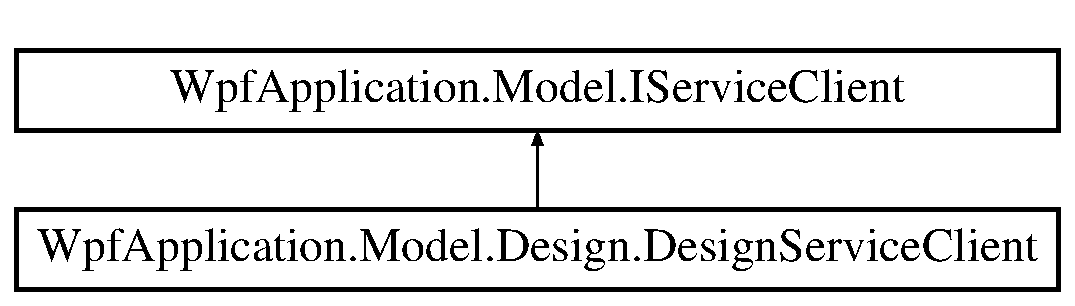
\includegraphics[height=2.000000cm]{class_wpf_application_1_1_model_1_1_design_1_1_design_service_client}
\end{center}
\end{figure}
\subsection*{Public Member Functions}
\begin{DoxyCompactItemize}
\item 
\hyperlink{class_wpf_application_1_1_model_1_1_client}{Client} \hyperlink{class_wpf_application_1_1_model_1_1_design_1_1_design_service_client_a53e0167efe1963da87880b2aad52f8d1}{Charger} ()
\item 
List$<$ \hyperlink{class_wpf_application_1_1_model_1_1_client}{Client} $>$ \hyperlink{class_wpf_application_1_1_model_1_1_design_1_1_design_service_client_adfe9e15a5cb29e6f1de7c6e30f494004}{Charger\-Tout} ()
\end{DoxyCompactItemize}


\subsection{Member Function Documentation}
\hypertarget{class_wpf_application_1_1_model_1_1_design_1_1_design_service_client_a53e0167efe1963da87880b2aad52f8d1}{\index{Wpf\-Application\-::\-Model\-::\-Design\-::\-Design\-Service\-Client@{Wpf\-Application\-::\-Model\-::\-Design\-::\-Design\-Service\-Client}!Charger@{Charger}}
\index{Charger@{Charger}!WpfApplication::Model::Design::DesignServiceClient@{Wpf\-Application\-::\-Model\-::\-Design\-::\-Design\-Service\-Client}}
\subsubsection[{Charger}]{\setlength{\rightskip}{0pt plus 5cm}{\bf Client} Wpf\-Application.\-Model.\-Design.\-Design\-Service\-Client.\-Charger (
\begin{DoxyParamCaption}
{}
\end{DoxyParamCaption}
)}}\label{class_wpf_application_1_1_model_1_1_design_1_1_design_service_client_a53e0167efe1963da87880b2aad52f8d1}


Implements \hyperlink{interface_wpf_application_1_1_model_1_1_i_service_client_ab513b6cf91c0d31cfe37004ac5cf7e1e}{Wpf\-Application.\-Model.\-I\-Service\-Client}.

\hypertarget{class_wpf_application_1_1_model_1_1_design_1_1_design_service_client_adfe9e15a5cb29e6f1de7c6e30f494004}{\index{Wpf\-Application\-::\-Model\-::\-Design\-::\-Design\-Service\-Client@{Wpf\-Application\-::\-Model\-::\-Design\-::\-Design\-Service\-Client}!Charger\-Tout@{Charger\-Tout}}
\index{Charger\-Tout@{Charger\-Tout}!WpfApplication::Model::Design::DesignServiceClient@{Wpf\-Application\-::\-Model\-::\-Design\-::\-Design\-Service\-Client}}
\subsubsection[{Charger\-Tout}]{\setlength{\rightskip}{0pt plus 5cm}List$<${\bf Client}$>$ Wpf\-Application.\-Model.\-Design.\-Design\-Service\-Client.\-Charger\-Tout (
\begin{DoxyParamCaption}
{}
\end{DoxyParamCaption}
)}}\label{class_wpf_application_1_1_model_1_1_design_1_1_design_service_client_adfe9e15a5cb29e6f1de7c6e30f494004}


Implements \hyperlink{interface_wpf_application_1_1_model_1_1_i_service_client_a40ae24e7195bb27667e26ed27319c3e5}{Wpf\-Application.\-Model.\-I\-Service\-Client}.



The documentation for this class was generated from the following file\-:\begin{DoxyCompactItemize}
\item 
C\-:/\-Users/dju/\-Documents/\-Visual Studio 2012/\-Projects/\-P\-P\-E/\-P\-P\-E3/\-Wpf\-Application/\-Model/\-Design/\hyperlink{_design_service_client_8cs}{Design\-Service\-Client.\-cs}\end{DoxyCompactItemize}

\hypertarget{class_model_1_1_d_i_r_e_c_t_e_u_r___r_e_g_i_o_n_a_l}{\section{Model.\-D\-I\-R\-E\-C\-T\-E\-U\-R\-\_\-\-R\-E\-G\-I\-O\-N\-A\-L Class Reference}
\label{class_model_1_1_d_i_r_e_c_t_e_u_r___r_e_g_i_o_n_a_l}\index{Model.\-D\-I\-R\-E\-C\-T\-E\-U\-R\-\_\-\-R\-E\-G\-I\-O\-N\-A\-L@{Model.\-D\-I\-R\-E\-C\-T\-E\-U\-R\-\_\-\-R\-E\-G\-I\-O\-N\-A\-L}}
}


Aucune documentation sur les métadonnées n'est disponible.  


Inheritance diagram for Model.\-D\-I\-R\-E\-C\-T\-E\-U\-R\-\_\-\-R\-E\-G\-I\-O\-N\-A\-L\-:\begin{figure}[H]
\begin{center}
\leavevmode
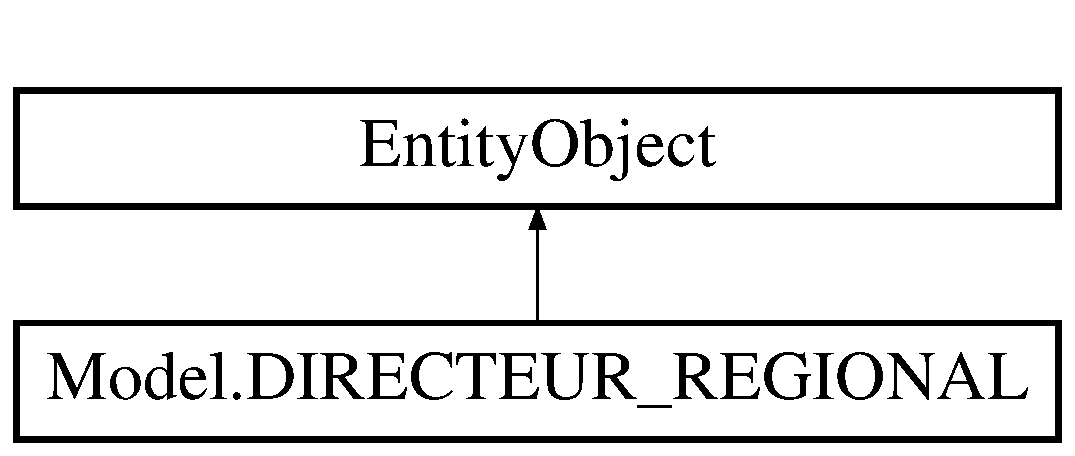
\includegraphics[height=2.000000cm]{class_model_1_1_d_i_r_e_c_t_e_u_r___r_e_g_i_o_n_a_l}
\end{center}
\end{figure}
\subsection*{Static Public Member Functions}
\begin{DoxyCompactItemize}
\item 
static \hyperlink{class_model_1_1_d_i_r_e_c_t_e_u_r___r_e_g_i_o_n_a_l}{D\-I\-R\-E\-C\-T\-E\-U\-R\-\_\-\-R\-E\-G\-I\-O\-N\-A\-L} \hyperlink{class_model_1_1_d_i_r_e_c_t_e_u_r___r_e_g_i_o_n_a_l_a819f70c009cbf1e34a0e7fb9d48ed221}{Create\-D\-I\-R\-E\-C\-T\-E\-U\-R\-\_\-\-R\-E\-G\-I\-O\-N\-A\-L} (global\-::\-System.\-Int32 \hyperlink{class_model_1_1_d_i_r_e_c_t_e_u_r___r_e_g_i_o_n_a_l_af8f929e9e0dd4f9a73d90d9f234a83d2}{matricule\-\_\-col\-\_\-dir})
\begin{DoxyCompactList}\small\item\em Créez un nouvel objet \hyperlink{class_model_1_1_d_i_r_e_c_t_e_u_r___r_e_g_i_o_n_a_l}{D\-I\-R\-E\-C\-T\-E\-U\-R\-\_\-\-R\-E\-G\-I\-O\-N\-A\-L}. \end{DoxyCompactList}\end{DoxyCompactItemize}
\subsection*{Properties}
\begin{DoxyCompactItemize}
\item 
global\-::\-System.\-Int32 \hyperlink{class_model_1_1_d_i_r_e_c_t_e_u_r___r_e_g_i_o_n_a_l_af8f929e9e0dd4f9a73d90d9f234a83d2}{matricule\-\_\-col\-\_\-dir}\hspace{0.3cm}{\ttfamily  \mbox{[}get, set\mbox{]}}
\begin{DoxyCompactList}\small\item\em Aucune documentation sur les métadonnées n'est disponible. \end{DoxyCompactList}\item 
\hyperlink{class_model_1_1_c_o_l_l_a_b_o_r_a_t_e_u_r}{C\-O\-L\-L\-A\-B\-O\-R\-A\-T\-E\-U\-R} \hyperlink{class_model_1_1_d_i_r_e_c_t_e_u_r___r_e_g_i_o_n_a_l_ab521033cf2f8ba34d4f8ac689c716eef}{C\-O\-L\-L\-A\-B\-O\-R\-A\-T\-E\-U\-R}\hspace{0.3cm}{\ttfamily  \mbox{[}get, set\mbox{]}}
\begin{DoxyCompactList}\small\item\em Aucune documentation sur les métadonnées n'est disponible. \end{DoxyCompactList}\item 
Entity\-Reference$<$ \hyperlink{class_model_1_1_c_o_l_l_a_b_o_r_a_t_e_u_r}{C\-O\-L\-L\-A\-B\-O\-R\-A\-T\-E\-U\-R} $>$ \hyperlink{class_model_1_1_d_i_r_e_c_t_e_u_r___r_e_g_i_o_n_a_l_a17398b2802e5c114de482c1ca1ab77a8}{C\-O\-L\-L\-A\-B\-O\-R\-A\-T\-E\-U\-R\-Reference}\hspace{0.3cm}{\ttfamily  \mbox{[}get, set\mbox{]}}
\begin{DoxyCompactList}\small\item\em Aucune documentation sur les métadonnées n'est disponible. \end{DoxyCompactList}\end{DoxyCompactItemize}


\subsection{Detailed Description}
Aucune documentation sur les métadonnées n'est disponible. 



\subsection{Member Function Documentation}
\hypertarget{class_model_1_1_d_i_r_e_c_t_e_u_r___r_e_g_i_o_n_a_l_a819f70c009cbf1e34a0e7fb9d48ed221}{\index{Model\-::\-D\-I\-R\-E\-C\-T\-E\-U\-R\-\_\-\-R\-E\-G\-I\-O\-N\-A\-L@{Model\-::\-D\-I\-R\-E\-C\-T\-E\-U\-R\-\_\-\-R\-E\-G\-I\-O\-N\-A\-L}!Create\-D\-I\-R\-E\-C\-T\-E\-U\-R\-\_\-\-R\-E\-G\-I\-O\-N\-A\-L@{Create\-D\-I\-R\-E\-C\-T\-E\-U\-R\-\_\-\-R\-E\-G\-I\-O\-N\-A\-L}}
\index{Create\-D\-I\-R\-E\-C\-T\-E\-U\-R\-\_\-\-R\-E\-G\-I\-O\-N\-A\-L@{Create\-D\-I\-R\-E\-C\-T\-E\-U\-R\-\_\-\-R\-E\-G\-I\-O\-N\-A\-L}!Model::DIRECTEUR_REGIONAL@{Model\-::\-D\-I\-R\-E\-C\-T\-E\-U\-R\-\_\-\-R\-E\-G\-I\-O\-N\-A\-L}}
\subsubsection[{Create\-D\-I\-R\-E\-C\-T\-E\-U\-R\-\_\-\-R\-E\-G\-I\-O\-N\-A\-L}]{\setlength{\rightskip}{0pt plus 5cm}static {\bf D\-I\-R\-E\-C\-T\-E\-U\-R\-\_\-\-R\-E\-G\-I\-O\-N\-A\-L} Model.\-D\-I\-R\-E\-C\-T\-E\-U\-R\-\_\-\-R\-E\-G\-I\-O\-N\-A\-L.\-Create\-D\-I\-R\-E\-C\-T\-E\-U\-R\-\_\-\-R\-E\-G\-I\-O\-N\-A\-L (
\begin{DoxyParamCaption}
\item[{global\-::\-System.\-Int32}]{matricule\-\_\-col\-\_\-dir}
\end{DoxyParamCaption}
)\hspace{0.3cm}{\ttfamily [static]}}}\label{class_model_1_1_d_i_r_e_c_t_e_u_r___r_e_g_i_o_n_a_l_a819f70c009cbf1e34a0e7fb9d48ed221}


Créez un nouvel objet \hyperlink{class_model_1_1_d_i_r_e_c_t_e_u_r___r_e_g_i_o_n_a_l}{D\-I\-R\-E\-C\-T\-E\-U\-R\-\_\-\-R\-E\-G\-I\-O\-N\-A\-L}. 


\begin{DoxyParams}{Parameters}
{\em matricule\-\_\-col\-\_\-dir} & Valeur initiale de la propriété matricule\-\_\-col\-\_\-dir.\\
\hline
\end{DoxyParams}


\subsection{Property Documentation}
\hypertarget{class_model_1_1_d_i_r_e_c_t_e_u_r___r_e_g_i_o_n_a_l_ab521033cf2f8ba34d4f8ac689c716eef}{\index{Model\-::\-D\-I\-R\-E\-C\-T\-E\-U\-R\-\_\-\-R\-E\-G\-I\-O\-N\-A\-L@{Model\-::\-D\-I\-R\-E\-C\-T\-E\-U\-R\-\_\-\-R\-E\-G\-I\-O\-N\-A\-L}!C\-O\-L\-L\-A\-B\-O\-R\-A\-T\-E\-U\-R@{C\-O\-L\-L\-A\-B\-O\-R\-A\-T\-E\-U\-R}}
\index{C\-O\-L\-L\-A\-B\-O\-R\-A\-T\-E\-U\-R@{C\-O\-L\-L\-A\-B\-O\-R\-A\-T\-E\-U\-R}!Model::DIRECTEUR_REGIONAL@{Model\-::\-D\-I\-R\-E\-C\-T\-E\-U\-R\-\_\-\-R\-E\-G\-I\-O\-N\-A\-L}}
\subsubsection[{C\-O\-L\-L\-A\-B\-O\-R\-A\-T\-E\-U\-R}]{\setlength{\rightskip}{0pt plus 5cm}{\bf C\-O\-L\-L\-A\-B\-O\-R\-A\-T\-E\-U\-R} Model.\-D\-I\-R\-E\-C\-T\-E\-U\-R\-\_\-\-R\-E\-G\-I\-O\-N\-A\-L.\-C\-O\-L\-L\-A\-B\-O\-R\-A\-T\-E\-U\-R\hspace{0.3cm}{\ttfamily [get]}, {\ttfamily [set]}}}\label{class_model_1_1_d_i_r_e_c_t_e_u_r___r_e_g_i_o_n_a_l_ab521033cf2f8ba34d4f8ac689c716eef}


Aucune documentation sur les métadonnées n'est disponible. 

\hypertarget{class_model_1_1_d_i_r_e_c_t_e_u_r___r_e_g_i_o_n_a_l_a17398b2802e5c114de482c1ca1ab77a8}{\index{Model\-::\-D\-I\-R\-E\-C\-T\-E\-U\-R\-\_\-\-R\-E\-G\-I\-O\-N\-A\-L@{Model\-::\-D\-I\-R\-E\-C\-T\-E\-U\-R\-\_\-\-R\-E\-G\-I\-O\-N\-A\-L}!C\-O\-L\-L\-A\-B\-O\-R\-A\-T\-E\-U\-R\-Reference@{C\-O\-L\-L\-A\-B\-O\-R\-A\-T\-E\-U\-R\-Reference}}
\index{C\-O\-L\-L\-A\-B\-O\-R\-A\-T\-E\-U\-R\-Reference@{C\-O\-L\-L\-A\-B\-O\-R\-A\-T\-E\-U\-R\-Reference}!Model::DIRECTEUR_REGIONAL@{Model\-::\-D\-I\-R\-E\-C\-T\-E\-U\-R\-\_\-\-R\-E\-G\-I\-O\-N\-A\-L}}
\subsubsection[{C\-O\-L\-L\-A\-B\-O\-R\-A\-T\-E\-U\-R\-Reference}]{\setlength{\rightskip}{0pt plus 5cm}Entity\-Reference$<${\bf C\-O\-L\-L\-A\-B\-O\-R\-A\-T\-E\-U\-R}$>$ Model.\-D\-I\-R\-E\-C\-T\-E\-U\-R\-\_\-\-R\-E\-G\-I\-O\-N\-A\-L.\-C\-O\-L\-L\-A\-B\-O\-R\-A\-T\-E\-U\-R\-Reference\hspace{0.3cm}{\ttfamily [get]}, {\ttfamily [set]}}}\label{class_model_1_1_d_i_r_e_c_t_e_u_r___r_e_g_i_o_n_a_l_a17398b2802e5c114de482c1ca1ab77a8}


Aucune documentation sur les métadonnées n'est disponible. 

\hypertarget{class_model_1_1_d_i_r_e_c_t_e_u_r___r_e_g_i_o_n_a_l_af8f929e9e0dd4f9a73d90d9f234a83d2}{\index{Model\-::\-D\-I\-R\-E\-C\-T\-E\-U\-R\-\_\-\-R\-E\-G\-I\-O\-N\-A\-L@{Model\-::\-D\-I\-R\-E\-C\-T\-E\-U\-R\-\_\-\-R\-E\-G\-I\-O\-N\-A\-L}!matricule\-\_\-col\-\_\-dir@{matricule\-\_\-col\-\_\-dir}}
\index{matricule\-\_\-col\-\_\-dir@{matricule\-\_\-col\-\_\-dir}!Model::DIRECTEUR_REGIONAL@{Model\-::\-D\-I\-R\-E\-C\-T\-E\-U\-R\-\_\-\-R\-E\-G\-I\-O\-N\-A\-L}}
\subsubsection[{matricule\-\_\-col\-\_\-dir}]{\setlength{\rightskip}{0pt plus 5cm}global.\-System.\-Int32 Model.\-D\-I\-R\-E\-C\-T\-E\-U\-R\-\_\-\-R\-E\-G\-I\-O\-N\-A\-L.\-matricule\-\_\-col\-\_\-dir\hspace{0.3cm}{\ttfamily [get]}, {\ttfamily [set]}}}\label{class_model_1_1_d_i_r_e_c_t_e_u_r___r_e_g_i_o_n_a_l_af8f929e9e0dd4f9a73d90d9f234a83d2}


Aucune documentation sur les métadonnées n'est disponible. 



The documentation for this class was generated from the following file\-:\begin{DoxyCompactItemize}
\item 
C\-:/\-Users/dju/\-Documents/\-Visual Studio 2012/\-Projects/\-P\-P\-E/\-P\-P\-E3/\-Model/\hyperlink{_model_bdd_sio_8_designer_8cs}{Model\-Bdd\-Sio.\-Designer.\-cs}\end{DoxyCompactItemize}

\hypertarget{class_model_1_1_d_o_s_a_g_e}{\section{Model.\-D\-O\-S\-A\-G\-E Class Reference}
\label{class_model_1_1_d_o_s_a_g_e}\index{Model.\-D\-O\-S\-A\-G\-E@{Model.\-D\-O\-S\-A\-G\-E}}
}


Aucune documentation sur les métadonnées n'est disponible.  


Inheritance diagram for Model.\-D\-O\-S\-A\-G\-E\-:\begin{figure}[H]
\begin{center}
\leavevmode
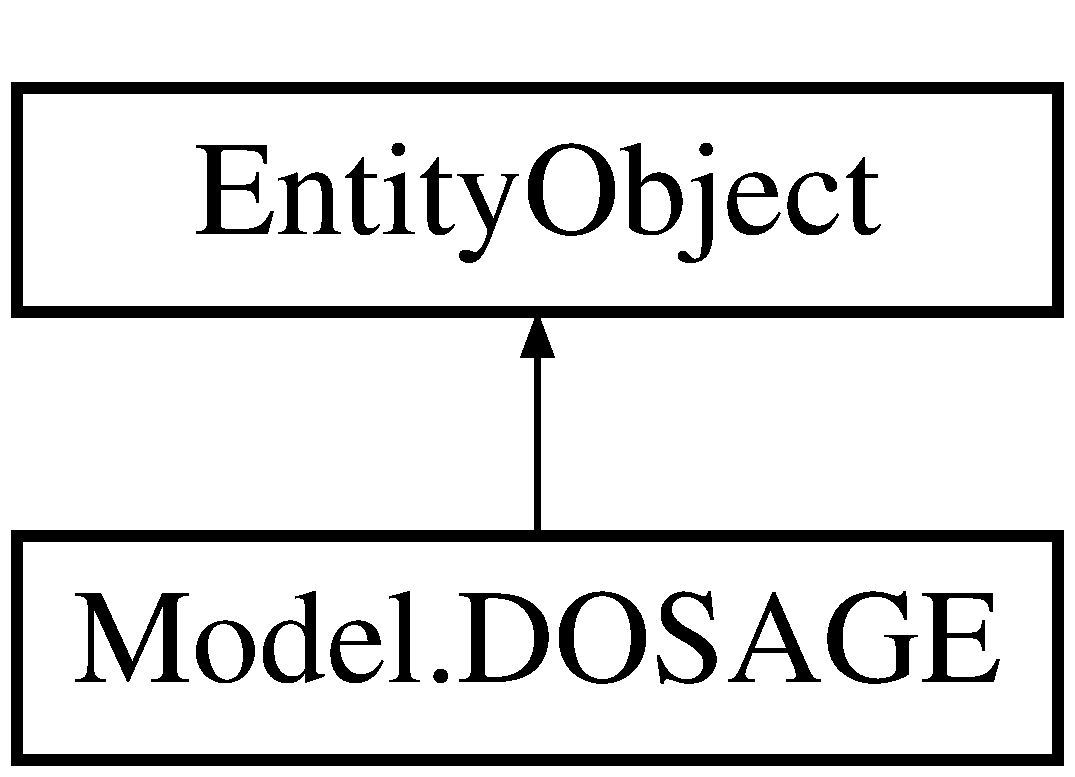
\includegraphics[height=2.000000cm]{class_model_1_1_d_o_s_a_g_e}
\end{center}
\end{figure}
\subsection*{Static Public Member Functions}
\begin{DoxyCompactItemize}
\item 
static \hyperlink{class_model_1_1_d_o_s_a_g_e}{D\-O\-S\-A\-G\-E} \hyperlink{class_model_1_1_d_o_s_a_g_e_ae142d476b20c913dde135f3e65fce332}{Create\-D\-O\-S\-A\-G\-E} (global\-::\-System.\-Int32 \hyperlink{class_model_1_1_d_o_s_a_g_e_af32ad785d5d3cdf43390c6a6f02d078a}{code\-\_\-dosage}, global\-::\-System.\-String \hyperlink{class_model_1_1_d_o_s_a_g_e_a3404cd2f5d068ae264fd6848e4baf4e5}{unite\-\_\-dosage}, global\-::\-System.\-Double \hyperlink{class_model_1_1_d_o_s_a_g_e_ac3bf6f580f1ebe8e492def33d2b8bcbc}{quantite\-\_\-dosage})
\begin{DoxyCompactList}\small\item\em Créez un nouvel objet \hyperlink{class_model_1_1_d_o_s_a_g_e}{D\-O\-S\-A\-G\-E}. \end{DoxyCompactList}\end{DoxyCompactItemize}
\subsection*{Properties}
\begin{DoxyCompactItemize}
\item 
global\-::\-System.\-Int32 \hyperlink{class_model_1_1_d_o_s_a_g_e_af32ad785d5d3cdf43390c6a6f02d078a}{code\-\_\-dosage}\hspace{0.3cm}{\ttfamily  \mbox{[}get, set\mbox{]}}
\begin{DoxyCompactList}\small\item\em Aucune documentation sur les métadonnées n'est disponible. \end{DoxyCompactList}\item 
global\-::\-System.\-String \hyperlink{class_model_1_1_d_o_s_a_g_e_a3404cd2f5d068ae264fd6848e4baf4e5}{unite\-\_\-dosage}\hspace{0.3cm}{\ttfamily  \mbox{[}get, set\mbox{]}}
\begin{DoxyCompactList}\small\item\em Aucune documentation sur les métadonnées n'est disponible. \end{DoxyCompactList}\item 
global\-::\-System.\-Double \hyperlink{class_model_1_1_d_o_s_a_g_e_ac3bf6f580f1ebe8e492def33d2b8bcbc}{quantite\-\_\-dosage}\hspace{0.3cm}{\ttfamily  \mbox{[}get, set\mbox{]}}
\begin{DoxyCompactList}\small\item\em Aucune documentation sur les métadonnées n'est disponible. \end{DoxyCompactList}\item 
Entity\-Collection$<$ \hyperlink{class_model_1_1_p_r_e_s_c_r_i_r_e}{P\-R\-E\-S\-C\-R\-I\-R\-E} $>$ \hyperlink{class_model_1_1_d_o_s_a_g_e_a98f3391689994e603d1b4e97b3e29f61}{P\-R\-E\-S\-C\-R\-I\-R\-E}\hspace{0.3cm}{\ttfamily  \mbox{[}get, set\mbox{]}}
\begin{DoxyCompactList}\small\item\em Aucune documentation sur les métadonnées n'est disponible. \end{DoxyCompactList}\end{DoxyCompactItemize}


\subsection{Detailed Description}
Aucune documentation sur les métadonnées n'est disponible. 



\subsection{Member Function Documentation}
\hypertarget{class_model_1_1_d_o_s_a_g_e_ae142d476b20c913dde135f3e65fce332}{\index{Model\-::\-D\-O\-S\-A\-G\-E@{Model\-::\-D\-O\-S\-A\-G\-E}!Create\-D\-O\-S\-A\-G\-E@{Create\-D\-O\-S\-A\-G\-E}}
\index{Create\-D\-O\-S\-A\-G\-E@{Create\-D\-O\-S\-A\-G\-E}!Model::DOSAGE@{Model\-::\-D\-O\-S\-A\-G\-E}}
\subsubsection[{Create\-D\-O\-S\-A\-G\-E}]{\setlength{\rightskip}{0pt plus 5cm}static {\bf D\-O\-S\-A\-G\-E} Model.\-D\-O\-S\-A\-G\-E.\-Create\-D\-O\-S\-A\-G\-E (
\begin{DoxyParamCaption}
\item[{global\-::\-System.\-Int32}]{code\-\_\-dosage, }
\item[{global\-::\-System.\-String}]{unite\-\_\-dosage, }
\item[{global\-::\-System.\-Double}]{quantite\-\_\-dosage}
\end{DoxyParamCaption}
)\hspace{0.3cm}{\ttfamily [static]}}}\label{class_model_1_1_d_o_s_a_g_e_ae142d476b20c913dde135f3e65fce332}


Créez un nouvel objet \hyperlink{class_model_1_1_d_o_s_a_g_e}{D\-O\-S\-A\-G\-E}. 


\begin{DoxyParams}{Parameters}
{\em code\-\_\-dosage} & Valeur initiale de la propriété code\-\_\-dosage.\\
\hline
{\em unite\-\_\-dosage} & Valeur initiale de la propriété unite\-\_\-dosage.\\
\hline
{\em quantite\-\_\-dosage} & Valeur initiale de la propriété quantite\-\_\-dosage.\\
\hline
\end{DoxyParams}


\subsection{Property Documentation}
\hypertarget{class_model_1_1_d_o_s_a_g_e_af32ad785d5d3cdf43390c6a6f02d078a}{\index{Model\-::\-D\-O\-S\-A\-G\-E@{Model\-::\-D\-O\-S\-A\-G\-E}!code\-\_\-dosage@{code\-\_\-dosage}}
\index{code\-\_\-dosage@{code\-\_\-dosage}!Model::DOSAGE@{Model\-::\-D\-O\-S\-A\-G\-E}}
\subsubsection[{code\-\_\-dosage}]{\setlength{\rightskip}{0pt plus 5cm}global.\-System.\-Int32 Model.\-D\-O\-S\-A\-G\-E.\-code\-\_\-dosage\hspace{0.3cm}{\ttfamily [get]}, {\ttfamily [set]}}}\label{class_model_1_1_d_o_s_a_g_e_af32ad785d5d3cdf43390c6a6f02d078a}


Aucune documentation sur les métadonnées n'est disponible. 

\hypertarget{class_model_1_1_d_o_s_a_g_e_a98f3391689994e603d1b4e97b3e29f61}{\index{Model\-::\-D\-O\-S\-A\-G\-E@{Model\-::\-D\-O\-S\-A\-G\-E}!P\-R\-E\-S\-C\-R\-I\-R\-E@{P\-R\-E\-S\-C\-R\-I\-R\-E}}
\index{P\-R\-E\-S\-C\-R\-I\-R\-E@{P\-R\-E\-S\-C\-R\-I\-R\-E}!Model::DOSAGE@{Model\-::\-D\-O\-S\-A\-G\-E}}
\subsubsection[{P\-R\-E\-S\-C\-R\-I\-R\-E}]{\setlength{\rightskip}{0pt plus 5cm}Entity\-Collection$<${\bf P\-R\-E\-S\-C\-R\-I\-R\-E}$>$ Model.\-D\-O\-S\-A\-G\-E.\-P\-R\-E\-S\-C\-R\-I\-R\-E\hspace{0.3cm}{\ttfamily [get]}, {\ttfamily [set]}}}\label{class_model_1_1_d_o_s_a_g_e_a98f3391689994e603d1b4e97b3e29f61}


Aucune documentation sur les métadonnées n'est disponible. 

\hypertarget{class_model_1_1_d_o_s_a_g_e_ac3bf6f580f1ebe8e492def33d2b8bcbc}{\index{Model\-::\-D\-O\-S\-A\-G\-E@{Model\-::\-D\-O\-S\-A\-G\-E}!quantite\-\_\-dosage@{quantite\-\_\-dosage}}
\index{quantite\-\_\-dosage@{quantite\-\_\-dosage}!Model::DOSAGE@{Model\-::\-D\-O\-S\-A\-G\-E}}
\subsubsection[{quantite\-\_\-dosage}]{\setlength{\rightskip}{0pt plus 5cm}global.\-System.\-Double Model.\-D\-O\-S\-A\-G\-E.\-quantite\-\_\-dosage\hspace{0.3cm}{\ttfamily [get]}, {\ttfamily [set]}}}\label{class_model_1_1_d_o_s_a_g_e_ac3bf6f580f1ebe8e492def33d2b8bcbc}


Aucune documentation sur les métadonnées n'est disponible. 

\hypertarget{class_model_1_1_d_o_s_a_g_e_a3404cd2f5d068ae264fd6848e4baf4e5}{\index{Model\-::\-D\-O\-S\-A\-G\-E@{Model\-::\-D\-O\-S\-A\-G\-E}!unite\-\_\-dosage@{unite\-\_\-dosage}}
\index{unite\-\_\-dosage@{unite\-\_\-dosage}!Model::DOSAGE@{Model\-::\-D\-O\-S\-A\-G\-E}}
\subsubsection[{unite\-\_\-dosage}]{\setlength{\rightskip}{0pt plus 5cm}global.\-System.\-String Model.\-D\-O\-S\-A\-G\-E.\-unite\-\_\-dosage\hspace{0.3cm}{\ttfamily [get]}, {\ttfamily [set]}}}\label{class_model_1_1_d_o_s_a_g_e_a3404cd2f5d068ae264fd6848e4baf4e5}


Aucune documentation sur les métadonnées n'est disponible. 



The documentation for this class was generated from the following file\-:\begin{DoxyCompactItemize}
\item 
C\-:/\-Users/dju/\-Documents/\-Visual Studio 2012/\-Projects/\-P\-P\-E/\-P\-P\-E3/\-Model/\hyperlink{_model_bdd_sio_8_designer_8cs}{Model\-Bdd\-Sio.\-Designer.\-cs}\end{DoxyCompactItemize}

\hypertarget{class_model_1_1_e_t_r_e___r_e_s_p_o_n_s_a_b_l_e}{\section{Model.\-E\-T\-R\-E\-\_\-\-R\-E\-S\-P\-O\-N\-S\-A\-B\-L\-E Class Reference}
\label{class_model_1_1_e_t_r_e___r_e_s_p_o_n_s_a_b_l_e}\index{Model.\-E\-T\-R\-E\-\_\-\-R\-E\-S\-P\-O\-N\-S\-A\-B\-L\-E@{Model.\-E\-T\-R\-E\-\_\-\-R\-E\-S\-P\-O\-N\-S\-A\-B\-L\-E}}
}


Aucune documentation sur les métadonnées n'est disponible.  


Inheritance diagram for Model.\-E\-T\-R\-E\-\_\-\-R\-E\-S\-P\-O\-N\-S\-A\-B\-L\-E\-:\begin{figure}[H]
\begin{center}
\leavevmode
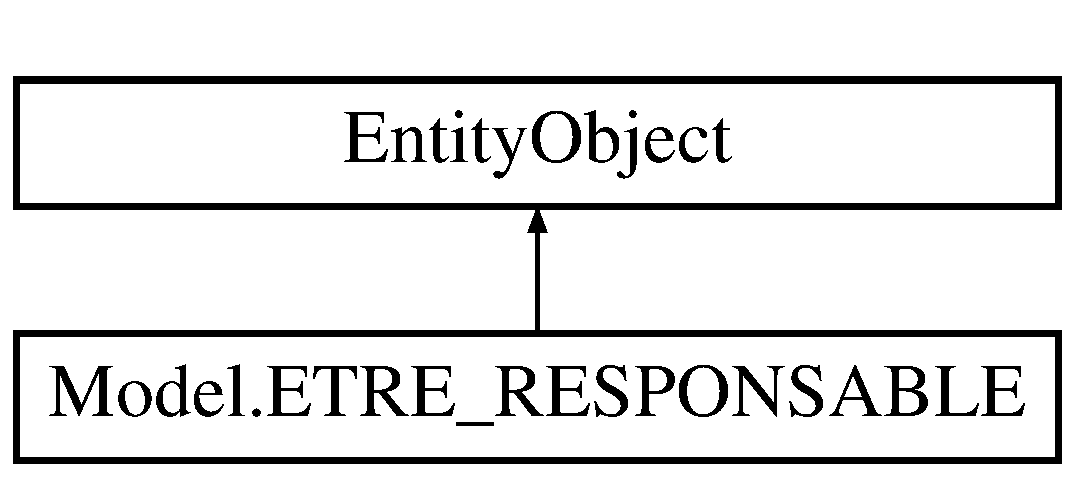
\includegraphics[height=2.000000cm]{class_model_1_1_e_t_r_e___r_e_s_p_o_n_s_a_b_l_e}
\end{center}
\end{figure}
\subsection*{Static Public Member Functions}
\begin{DoxyCompactItemize}
\item 
static \hyperlink{class_model_1_1_e_t_r_e___r_e_s_p_o_n_s_a_b_l_e}{E\-T\-R\-E\-\_\-\-R\-E\-S\-P\-O\-N\-S\-A\-B\-L\-E} \hyperlink{class_model_1_1_e_t_r_e___r_e_s_p_o_n_s_a_b_l_e_a4dc6c16664e77615ea058c1d1c212053}{Create\-E\-T\-R\-E\-\_\-\-R\-E\-S\-P\-O\-N\-S\-A\-B\-L\-E} (global\-::\-System.\-Int32 \hyperlink{class_model_1_1_e_t_r_e___r_e_s_p_o_n_s_a_b_l_e_a91950cf430a908f316fe4273dd78ab88}{matricule\-\_\-col\-\_\-etr}, global\-::\-System.\-String \hyperlink{class_model_1_1_e_t_r_e___r_e_s_p_o_n_s_a_b_l_e_a30b273a91b5e42411cf4022a07490c2e}{code\-\_\-secteur}, global\-::\-System.\-Date\-Time j\-J\-M\-M\-A\-A\-A\-A\-\_\-\-F\-I\-N, global\-::\-System.\-Date\-Time j\-J\-M\-M\-A\-A\-A\-A\-\_\-\-D\-E\-B)
\begin{DoxyCompactList}\small\item\em Créez un nouvel objet \hyperlink{class_model_1_1_e_t_r_e___r_e_s_p_o_n_s_a_b_l_e}{E\-T\-R\-E\-\_\-\-R\-E\-S\-P\-O\-N\-S\-A\-B\-L\-E}. \end{DoxyCompactList}\end{DoxyCompactItemize}
\subsection*{Properties}
\begin{DoxyCompactItemize}
\item 
global\-::\-System.\-Int32 \hyperlink{class_model_1_1_e_t_r_e___r_e_s_p_o_n_s_a_b_l_e_a91950cf430a908f316fe4273dd78ab88}{matricule\-\_\-col\-\_\-etr}\hspace{0.3cm}{\ttfamily  \mbox{[}get, set\mbox{]}}
\begin{DoxyCompactList}\small\item\em Aucune documentation sur les métadonnées n'est disponible. \end{DoxyCompactList}\item 
global\-::\-System.\-String \hyperlink{class_model_1_1_e_t_r_e___r_e_s_p_o_n_s_a_b_l_e_a30b273a91b5e42411cf4022a07490c2e}{code\-\_\-secteur}\hspace{0.3cm}{\ttfamily  \mbox{[}get, set\mbox{]}}
\begin{DoxyCompactList}\small\item\em Aucune documentation sur les métadonnées n'est disponible. \end{DoxyCompactList}\item 
global\-::\-System.\-Date\-Time \hyperlink{class_model_1_1_e_t_r_e___r_e_s_p_o_n_s_a_b_l_e_aeaa7b22df873713292df37af00ba56ca}{J\-J\-M\-M\-A\-A\-A\-A\-\_\-\-F\-I\-N}\hspace{0.3cm}{\ttfamily  \mbox{[}get, set\mbox{]}}
\begin{DoxyCompactList}\small\item\em Aucune documentation sur les métadonnées n'est disponible. \end{DoxyCompactList}\item 
global\-::\-System.\-Date\-Time \hyperlink{class_model_1_1_e_t_r_e___r_e_s_p_o_n_s_a_b_l_e_a92345b0b6cee5b2742df44b3a0c85ecb}{J\-J\-M\-M\-A\-A\-A\-A\-\_\-\-D\-E\-B}\hspace{0.3cm}{\ttfamily  \mbox{[}get, set\mbox{]}}
\begin{DoxyCompactList}\small\item\em Aucune documentation sur les métadonnées n'est disponible. \end{DoxyCompactList}\item 
\hyperlink{class_model_1_1_c_a_l_e_n_d_r_i_e_r}{C\-A\-L\-E\-N\-D\-R\-I\-E\-R} \hyperlink{class_model_1_1_e_t_r_e___r_e_s_p_o_n_s_a_b_l_e_a83b6740c4abe967975f20f4b3139daf2}{C\-A\-L\-E\-N\-D\-R\-I\-E\-R}\hspace{0.3cm}{\ttfamily  \mbox{[}get, set\mbox{]}}
\begin{DoxyCompactList}\small\item\em Aucune documentation sur les métadonnées n'est disponible. \end{DoxyCompactList}\item 
Entity\-Reference$<$ \hyperlink{class_model_1_1_c_a_l_e_n_d_r_i_e_r}{C\-A\-L\-E\-N\-D\-R\-I\-E\-R} $>$ \hyperlink{class_model_1_1_e_t_r_e___r_e_s_p_o_n_s_a_b_l_e_a865fabbad6013698e39e4039dacd62be}{C\-A\-L\-E\-N\-D\-R\-I\-E\-R\-Reference}\hspace{0.3cm}{\ttfamily  \mbox{[}get, set\mbox{]}}
\begin{DoxyCompactList}\small\item\em Aucune documentation sur les métadonnées n'est disponible. \end{DoxyCompactList}\item 
\hyperlink{class_model_1_1_c_o_l_l_a_b_o_r_a_t_e_u_r}{C\-O\-L\-L\-A\-B\-O\-R\-A\-T\-E\-U\-R} \hyperlink{class_model_1_1_e_t_r_e___r_e_s_p_o_n_s_a_b_l_e_ad37e4916b9d01b522e7dee13ea668f2f}{C\-O\-L\-L\-A\-B\-O\-R\-A\-T\-E\-U\-R}\hspace{0.3cm}{\ttfamily  \mbox{[}get, set\mbox{]}}
\begin{DoxyCompactList}\small\item\em Aucune documentation sur les métadonnées n'est disponible. \end{DoxyCompactList}\item 
Entity\-Reference$<$ \hyperlink{class_model_1_1_c_o_l_l_a_b_o_r_a_t_e_u_r}{C\-O\-L\-L\-A\-B\-O\-R\-A\-T\-E\-U\-R} $>$ \hyperlink{class_model_1_1_e_t_r_e___r_e_s_p_o_n_s_a_b_l_e_a1dd54529ec10369d8720c52243162189}{C\-O\-L\-L\-A\-B\-O\-R\-A\-T\-E\-U\-R\-Reference}\hspace{0.3cm}{\ttfamily  \mbox{[}get, set\mbox{]}}
\begin{DoxyCompactList}\small\item\em Aucune documentation sur les métadonnées n'est disponible. \end{DoxyCompactList}\item 
\hyperlink{class_model_1_1_s_e_c_t_e_u_r}{S\-E\-C\-T\-E\-U\-R} \hyperlink{class_model_1_1_e_t_r_e___r_e_s_p_o_n_s_a_b_l_e_afc83419e745174726df079da891c6973}{S\-E\-C\-T\-E\-U\-R}\hspace{0.3cm}{\ttfamily  \mbox{[}get, set\mbox{]}}
\begin{DoxyCompactList}\small\item\em Aucune documentation sur les métadonnées n'est disponible. \end{DoxyCompactList}\item 
Entity\-Reference$<$ \hyperlink{class_model_1_1_s_e_c_t_e_u_r}{S\-E\-C\-T\-E\-U\-R} $>$ \hyperlink{class_model_1_1_e_t_r_e___r_e_s_p_o_n_s_a_b_l_e_a87465cb676675c817cef32ad96f182e3}{S\-E\-C\-T\-E\-U\-R\-Reference}\hspace{0.3cm}{\ttfamily  \mbox{[}get, set\mbox{]}}
\begin{DoxyCompactList}\small\item\em Aucune documentation sur les métadonnées n'est disponible. \end{DoxyCompactList}\end{DoxyCompactItemize}


\subsection{Detailed Description}
Aucune documentation sur les métadonnées n'est disponible. 



\subsection{Member Function Documentation}
\hypertarget{class_model_1_1_e_t_r_e___r_e_s_p_o_n_s_a_b_l_e_a4dc6c16664e77615ea058c1d1c212053}{\index{Model\-::\-E\-T\-R\-E\-\_\-\-R\-E\-S\-P\-O\-N\-S\-A\-B\-L\-E@{Model\-::\-E\-T\-R\-E\-\_\-\-R\-E\-S\-P\-O\-N\-S\-A\-B\-L\-E}!Create\-E\-T\-R\-E\-\_\-\-R\-E\-S\-P\-O\-N\-S\-A\-B\-L\-E@{Create\-E\-T\-R\-E\-\_\-\-R\-E\-S\-P\-O\-N\-S\-A\-B\-L\-E}}
\index{Create\-E\-T\-R\-E\-\_\-\-R\-E\-S\-P\-O\-N\-S\-A\-B\-L\-E@{Create\-E\-T\-R\-E\-\_\-\-R\-E\-S\-P\-O\-N\-S\-A\-B\-L\-E}!Model::ETRE_RESPONSABLE@{Model\-::\-E\-T\-R\-E\-\_\-\-R\-E\-S\-P\-O\-N\-S\-A\-B\-L\-E}}
\subsubsection[{Create\-E\-T\-R\-E\-\_\-\-R\-E\-S\-P\-O\-N\-S\-A\-B\-L\-E}]{\setlength{\rightskip}{0pt plus 5cm}static {\bf E\-T\-R\-E\-\_\-\-R\-E\-S\-P\-O\-N\-S\-A\-B\-L\-E} Model.\-E\-T\-R\-E\-\_\-\-R\-E\-S\-P\-O\-N\-S\-A\-B\-L\-E.\-Create\-E\-T\-R\-E\-\_\-\-R\-E\-S\-P\-O\-N\-S\-A\-B\-L\-E (
\begin{DoxyParamCaption}
\item[{global\-::\-System.\-Int32}]{matricule\-\_\-col\-\_\-etr, }
\item[{global\-::\-System.\-String}]{code\-\_\-secteur, }
\item[{global\-::\-System.\-Date\-Time}]{j\-J\-M\-M\-A\-A\-A\-A\-\_\-\-F\-I\-N, }
\item[{global\-::\-System.\-Date\-Time}]{j\-J\-M\-M\-A\-A\-A\-A\-\_\-\-D\-E\-B}
\end{DoxyParamCaption}
)\hspace{0.3cm}{\ttfamily [static]}}}\label{class_model_1_1_e_t_r_e___r_e_s_p_o_n_s_a_b_l_e_a4dc6c16664e77615ea058c1d1c212053}


Créez un nouvel objet \hyperlink{class_model_1_1_e_t_r_e___r_e_s_p_o_n_s_a_b_l_e}{E\-T\-R\-E\-\_\-\-R\-E\-S\-P\-O\-N\-S\-A\-B\-L\-E}. 


\begin{DoxyParams}{Parameters}
{\em matricule\-\_\-col\-\_\-etr} & Valeur initiale de la propriété matricule\-\_\-col\-\_\-etr.\\
\hline
{\em code\-\_\-secteur} & Valeur initiale de la propriété code\-\_\-secteur.\\
\hline
{\em j\-J\-M\-M\-A\-A\-A\-A\-\_\-\-F\-I\-N} & Valeur initiale de la propriété J\-J\-M\-M\-A\-A\-A\-A\-\_\-\-F\-I\-N.\\
\hline
{\em j\-J\-M\-M\-A\-A\-A\-A\-\_\-\-D\-E\-B} & Valeur initiale de la propriété J\-J\-M\-M\-A\-A\-A\-A\-\_\-\-D\-E\-B.\\
\hline
\end{DoxyParams}


\subsection{Property Documentation}
\hypertarget{class_model_1_1_e_t_r_e___r_e_s_p_o_n_s_a_b_l_e_a83b6740c4abe967975f20f4b3139daf2}{\index{Model\-::\-E\-T\-R\-E\-\_\-\-R\-E\-S\-P\-O\-N\-S\-A\-B\-L\-E@{Model\-::\-E\-T\-R\-E\-\_\-\-R\-E\-S\-P\-O\-N\-S\-A\-B\-L\-E}!C\-A\-L\-E\-N\-D\-R\-I\-E\-R@{C\-A\-L\-E\-N\-D\-R\-I\-E\-R}}
\index{C\-A\-L\-E\-N\-D\-R\-I\-E\-R@{C\-A\-L\-E\-N\-D\-R\-I\-E\-R}!Model::ETRE_RESPONSABLE@{Model\-::\-E\-T\-R\-E\-\_\-\-R\-E\-S\-P\-O\-N\-S\-A\-B\-L\-E}}
\subsubsection[{C\-A\-L\-E\-N\-D\-R\-I\-E\-R}]{\setlength{\rightskip}{0pt plus 5cm}{\bf C\-A\-L\-E\-N\-D\-R\-I\-E\-R} Model.\-E\-T\-R\-E\-\_\-\-R\-E\-S\-P\-O\-N\-S\-A\-B\-L\-E.\-C\-A\-L\-E\-N\-D\-R\-I\-E\-R\hspace{0.3cm}{\ttfamily [get]}, {\ttfamily [set]}}}\label{class_model_1_1_e_t_r_e___r_e_s_p_o_n_s_a_b_l_e_a83b6740c4abe967975f20f4b3139daf2}


Aucune documentation sur les métadonnées n'est disponible. 

\hypertarget{class_model_1_1_e_t_r_e___r_e_s_p_o_n_s_a_b_l_e_a865fabbad6013698e39e4039dacd62be}{\index{Model\-::\-E\-T\-R\-E\-\_\-\-R\-E\-S\-P\-O\-N\-S\-A\-B\-L\-E@{Model\-::\-E\-T\-R\-E\-\_\-\-R\-E\-S\-P\-O\-N\-S\-A\-B\-L\-E}!C\-A\-L\-E\-N\-D\-R\-I\-E\-R\-Reference@{C\-A\-L\-E\-N\-D\-R\-I\-E\-R\-Reference}}
\index{C\-A\-L\-E\-N\-D\-R\-I\-E\-R\-Reference@{C\-A\-L\-E\-N\-D\-R\-I\-E\-R\-Reference}!Model::ETRE_RESPONSABLE@{Model\-::\-E\-T\-R\-E\-\_\-\-R\-E\-S\-P\-O\-N\-S\-A\-B\-L\-E}}
\subsubsection[{C\-A\-L\-E\-N\-D\-R\-I\-E\-R\-Reference}]{\setlength{\rightskip}{0pt plus 5cm}Entity\-Reference$<${\bf C\-A\-L\-E\-N\-D\-R\-I\-E\-R}$>$ Model.\-E\-T\-R\-E\-\_\-\-R\-E\-S\-P\-O\-N\-S\-A\-B\-L\-E.\-C\-A\-L\-E\-N\-D\-R\-I\-E\-R\-Reference\hspace{0.3cm}{\ttfamily [get]}, {\ttfamily [set]}}}\label{class_model_1_1_e_t_r_e___r_e_s_p_o_n_s_a_b_l_e_a865fabbad6013698e39e4039dacd62be}


Aucune documentation sur les métadonnées n'est disponible. 

\hypertarget{class_model_1_1_e_t_r_e___r_e_s_p_o_n_s_a_b_l_e_a30b273a91b5e42411cf4022a07490c2e}{\index{Model\-::\-E\-T\-R\-E\-\_\-\-R\-E\-S\-P\-O\-N\-S\-A\-B\-L\-E@{Model\-::\-E\-T\-R\-E\-\_\-\-R\-E\-S\-P\-O\-N\-S\-A\-B\-L\-E}!code\-\_\-secteur@{code\-\_\-secteur}}
\index{code\-\_\-secteur@{code\-\_\-secteur}!Model::ETRE_RESPONSABLE@{Model\-::\-E\-T\-R\-E\-\_\-\-R\-E\-S\-P\-O\-N\-S\-A\-B\-L\-E}}
\subsubsection[{code\-\_\-secteur}]{\setlength{\rightskip}{0pt plus 5cm}global.\-System.\-String Model.\-E\-T\-R\-E\-\_\-\-R\-E\-S\-P\-O\-N\-S\-A\-B\-L\-E.\-code\-\_\-secteur\hspace{0.3cm}{\ttfamily [get]}, {\ttfamily [set]}}}\label{class_model_1_1_e_t_r_e___r_e_s_p_o_n_s_a_b_l_e_a30b273a91b5e42411cf4022a07490c2e}


Aucune documentation sur les métadonnées n'est disponible. 

\hypertarget{class_model_1_1_e_t_r_e___r_e_s_p_o_n_s_a_b_l_e_ad37e4916b9d01b522e7dee13ea668f2f}{\index{Model\-::\-E\-T\-R\-E\-\_\-\-R\-E\-S\-P\-O\-N\-S\-A\-B\-L\-E@{Model\-::\-E\-T\-R\-E\-\_\-\-R\-E\-S\-P\-O\-N\-S\-A\-B\-L\-E}!C\-O\-L\-L\-A\-B\-O\-R\-A\-T\-E\-U\-R@{C\-O\-L\-L\-A\-B\-O\-R\-A\-T\-E\-U\-R}}
\index{C\-O\-L\-L\-A\-B\-O\-R\-A\-T\-E\-U\-R@{C\-O\-L\-L\-A\-B\-O\-R\-A\-T\-E\-U\-R}!Model::ETRE_RESPONSABLE@{Model\-::\-E\-T\-R\-E\-\_\-\-R\-E\-S\-P\-O\-N\-S\-A\-B\-L\-E}}
\subsubsection[{C\-O\-L\-L\-A\-B\-O\-R\-A\-T\-E\-U\-R}]{\setlength{\rightskip}{0pt plus 5cm}{\bf C\-O\-L\-L\-A\-B\-O\-R\-A\-T\-E\-U\-R} Model.\-E\-T\-R\-E\-\_\-\-R\-E\-S\-P\-O\-N\-S\-A\-B\-L\-E.\-C\-O\-L\-L\-A\-B\-O\-R\-A\-T\-E\-U\-R\hspace{0.3cm}{\ttfamily [get]}, {\ttfamily [set]}}}\label{class_model_1_1_e_t_r_e___r_e_s_p_o_n_s_a_b_l_e_ad37e4916b9d01b522e7dee13ea668f2f}


Aucune documentation sur les métadonnées n'est disponible. 

\hypertarget{class_model_1_1_e_t_r_e___r_e_s_p_o_n_s_a_b_l_e_a1dd54529ec10369d8720c52243162189}{\index{Model\-::\-E\-T\-R\-E\-\_\-\-R\-E\-S\-P\-O\-N\-S\-A\-B\-L\-E@{Model\-::\-E\-T\-R\-E\-\_\-\-R\-E\-S\-P\-O\-N\-S\-A\-B\-L\-E}!C\-O\-L\-L\-A\-B\-O\-R\-A\-T\-E\-U\-R\-Reference@{C\-O\-L\-L\-A\-B\-O\-R\-A\-T\-E\-U\-R\-Reference}}
\index{C\-O\-L\-L\-A\-B\-O\-R\-A\-T\-E\-U\-R\-Reference@{C\-O\-L\-L\-A\-B\-O\-R\-A\-T\-E\-U\-R\-Reference}!Model::ETRE_RESPONSABLE@{Model\-::\-E\-T\-R\-E\-\_\-\-R\-E\-S\-P\-O\-N\-S\-A\-B\-L\-E}}
\subsubsection[{C\-O\-L\-L\-A\-B\-O\-R\-A\-T\-E\-U\-R\-Reference}]{\setlength{\rightskip}{0pt plus 5cm}Entity\-Reference$<${\bf C\-O\-L\-L\-A\-B\-O\-R\-A\-T\-E\-U\-R}$>$ Model.\-E\-T\-R\-E\-\_\-\-R\-E\-S\-P\-O\-N\-S\-A\-B\-L\-E.\-C\-O\-L\-L\-A\-B\-O\-R\-A\-T\-E\-U\-R\-Reference\hspace{0.3cm}{\ttfamily [get]}, {\ttfamily [set]}}}\label{class_model_1_1_e_t_r_e___r_e_s_p_o_n_s_a_b_l_e_a1dd54529ec10369d8720c52243162189}


Aucune documentation sur les métadonnées n'est disponible. 

\hypertarget{class_model_1_1_e_t_r_e___r_e_s_p_o_n_s_a_b_l_e_a92345b0b6cee5b2742df44b3a0c85ecb}{\index{Model\-::\-E\-T\-R\-E\-\_\-\-R\-E\-S\-P\-O\-N\-S\-A\-B\-L\-E@{Model\-::\-E\-T\-R\-E\-\_\-\-R\-E\-S\-P\-O\-N\-S\-A\-B\-L\-E}!J\-J\-M\-M\-A\-A\-A\-A\-\_\-\-D\-E\-B@{J\-J\-M\-M\-A\-A\-A\-A\-\_\-\-D\-E\-B}}
\index{J\-J\-M\-M\-A\-A\-A\-A\-\_\-\-D\-E\-B@{J\-J\-M\-M\-A\-A\-A\-A\-\_\-\-D\-E\-B}!Model::ETRE_RESPONSABLE@{Model\-::\-E\-T\-R\-E\-\_\-\-R\-E\-S\-P\-O\-N\-S\-A\-B\-L\-E}}
\subsubsection[{J\-J\-M\-M\-A\-A\-A\-A\-\_\-\-D\-E\-B}]{\setlength{\rightskip}{0pt plus 5cm}global.\-System.\-Date\-Time Model.\-E\-T\-R\-E\-\_\-\-R\-E\-S\-P\-O\-N\-S\-A\-B\-L\-E.\-J\-J\-M\-M\-A\-A\-A\-A\-\_\-\-D\-E\-B\hspace{0.3cm}{\ttfamily [get]}, {\ttfamily [set]}}}\label{class_model_1_1_e_t_r_e___r_e_s_p_o_n_s_a_b_l_e_a92345b0b6cee5b2742df44b3a0c85ecb}


Aucune documentation sur les métadonnées n'est disponible. 

\hypertarget{class_model_1_1_e_t_r_e___r_e_s_p_o_n_s_a_b_l_e_aeaa7b22df873713292df37af00ba56ca}{\index{Model\-::\-E\-T\-R\-E\-\_\-\-R\-E\-S\-P\-O\-N\-S\-A\-B\-L\-E@{Model\-::\-E\-T\-R\-E\-\_\-\-R\-E\-S\-P\-O\-N\-S\-A\-B\-L\-E}!J\-J\-M\-M\-A\-A\-A\-A\-\_\-\-F\-I\-N@{J\-J\-M\-M\-A\-A\-A\-A\-\_\-\-F\-I\-N}}
\index{J\-J\-M\-M\-A\-A\-A\-A\-\_\-\-F\-I\-N@{J\-J\-M\-M\-A\-A\-A\-A\-\_\-\-F\-I\-N}!Model::ETRE_RESPONSABLE@{Model\-::\-E\-T\-R\-E\-\_\-\-R\-E\-S\-P\-O\-N\-S\-A\-B\-L\-E}}
\subsubsection[{J\-J\-M\-M\-A\-A\-A\-A\-\_\-\-F\-I\-N}]{\setlength{\rightskip}{0pt plus 5cm}global.\-System.\-Date\-Time Model.\-E\-T\-R\-E\-\_\-\-R\-E\-S\-P\-O\-N\-S\-A\-B\-L\-E.\-J\-J\-M\-M\-A\-A\-A\-A\-\_\-\-F\-I\-N\hspace{0.3cm}{\ttfamily [get]}, {\ttfamily [set]}}}\label{class_model_1_1_e_t_r_e___r_e_s_p_o_n_s_a_b_l_e_aeaa7b22df873713292df37af00ba56ca}


Aucune documentation sur les métadonnées n'est disponible. 

\hypertarget{class_model_1_1_e_t_r_e___r_e_s_p_o_n_s_a_b_l_e_a91950cf430a908f316fe4273dd78ab88}{\index{Model\-::\-E\-T\-R\-E\-\_\-\-R\-E\-S\-P\-O\-N\-S\-A\-B\-L\-E@{Model\-::\-E\-T\-R\-E\-\_\-\-R\-E\-S\-P\-O\-N\-S\-A\-B\-L\-E}!matricule\-\_\-col\-\_\-etr@{matricule\-\_\-col\-\_\-etr}}
\index{matricule\-\_\-col\-\_\-etr@{matricule\-\_\-col\-\_\-etr}!Model::ETRE_RESPONSABLE@{Model\-::\-E\-T\-R\-E\-\_\-\-R\-E\-S\-P\-O\-N\-S\-A\-B\-L\-E}}
\subsubsection[{matricule\-\_\-col\-\_\-etr}]{\setlength{\rightskip}{0pt plus 5cm}global.\-System.\-Int32 Model.\-E\-T\-R\-E\-\_\-\-R\-E\-S\-P\-O\-N\-S\-A\-B\-L\-E.\-matricule\-\_\-col\-\_\-etr\hspace{0.3cm}{\ttfamily [get]}, {\ttfamily [set]}}}\label{class_model_1_1_e_t_r_e___r_e_s_p_o_n_s_a_b_l_e_a91950cf430a908f316fe4273dd78ab88}


Aucune documentation sur les métadonnées n'est disponible. 

\hypertarget{class_model_1_1_e_t_r_e___r_e_s_p_o_n_s_a_b_l_e_afc83419e745174726df079da891c6973}{\index{Model\-::\-E\-T\-R\-E\-\_\-\-R\-E\-S\-P\-O\-N\-S\-A\-B\-L\-E@{Model\-::\-E\-T\-R\-E\-\_\-\-R\-E\-S\-P\-O\-N\-S\-A\-B\-L\-E}!S\-E\-C\-T\-E\-U\-R@{S\-E\-C\-T\-E\-U\-R}}
\index{S\-E\-C\-T\-E\-U\-R@{S\-E\-C\-T\-E\-U\-R}!Model::ETRE_RESPONSABLE@{Model\-::\-E\-T\-R\-E\-\_\-\-R\-E\-S\-P\-O\-N\-S\-A\-B\-L\-E}}
\subsubsection[{S\-E\-C\-T\-E\-U\-R}]{\setlength{\rightskip}{0pt plus 5cm}{\bf S\-E\-C\-T\-E\-U\-R} Model.\-E\-T\-R\-E\-\_\-\-R\-E\-S\-P\-O\-N\-S\-A\-B\-L\-E.\-S\-E\-C\-T\-E\-U\-R\hspace{0.3cm}{\ttfamily [get]}, {\ttfamily [set]}}}\label{class_model_1_1_e_t_r_e___r_e_s_p_o_n_s_a_b_l_e_afc83419e745174726df079da891c6973}


Aucune documentation sur les métadonnées n'est disponible. 

\hypertarget{class_model_1_1_e_t_r_e___r_e_s_p_o_n_s_a_b_l_e_a87465cb676675c817cef32ad96f182e3}{\index{Model\-::\-E\-T\-R\-E\-\_\-\-R\-E\-S\-P\-O\-N\-S\-A\-B\-L\-E@{Model\-::\-E\-T\-R\-E\-\_\-\-R\-E\-S\-P\-O\-N\-S\-A\-B\-L\-E}!S\-E\-C\-T\-E\-U\-R\-Reference@{S\-E\-C\-T\-E\-U\-R\-Reference}}
\index{S\-E\-C\-T\-E\-U\-R\-Reference@{S\-E\-C\-T\-E\-U\-R\-Reference}!Model::ETRE_RESPONSABLE@{Model\-::\-E\-T\-R\-E\-\_\-\-R\-E\-S\-P\-O\-N\-S\-A\-B\-L\-E}}
\subsubsection[{S\-E\-C\-T\-E\-U\-R\-Reference}]{\setlength{\rightskip}{0pt plus 5cm}Entity\-Reference$<${\bf S\-E\-C\-T\-E\-U\-R}$>$ Model.\-E\-T\-R\-E\-\_\-\-R\-E\-S\-P\-O\-N\-S\-A\-B\-L\-E.\-S\-E\-C\-T\-E\-U\-R\-Reference\hspace{0.3cm}{\ttfamily [get]}, {\ttfamily [set]}}}\label{class_model_1_1_e_t_r_e___r_e_s_p_o_n_s_a_b_l_e_a87465cb676675c817cef32ad96f182e3}


Aucune documentation sur les métadonnées n'est disponible. 



The documentation for this class was generated from the following file\-:\begin{DoxyCompactItemize}
\item 
C\-:/\-Users/dju/\-Documents/\-Visual Studio 2012/\-Projects/\-P\-P\-E/\-P\-P\-E3/\-Model/\hyperlink{_model_bdd_sio_8_designer_8cs}{Model\-Bdd\-Sio.\-Designer.\-cs}\end{DoxyCompactItemize}

\hypertarget{class_model_1_1_f_a_m_i_l_l_e}{\section{Model.\-F\-A\-M\-I\-L\-L\-E Class Reference}
\label{class_model_1_1_f_a_m_i_l_l_e}\index{Model.\-F\-A\-M\-I\-L\-L\-E@{Model.\-F\-A\-M\-I\-L\-L\-E}}
}


Aucune documentation sur les métadonnées n'est disponible.  


Inheritance diagram for Model.\-F\-A\-M\-I\-L\-L\-E\-:\begin{figure}[H]
\begin{center}
\leavevmode
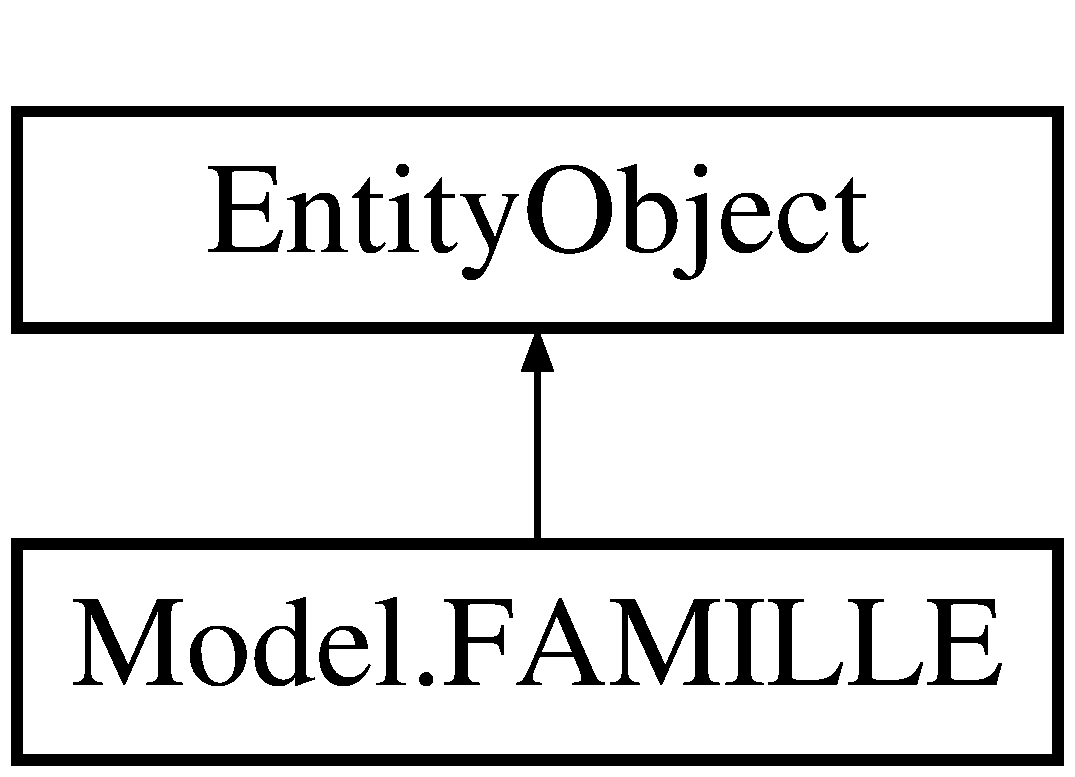
\includegraphics[height=2.000000cm]{class_model_1_1_f_a_m_i_l_l_e}
\end{center}
\end{figure}
\subsection*{Static Public Member Functions}
\begin{DoxyCompactItemize}
\item 
static \hyperlink{class_model_1_1_f_a_m_i_l_l_e}{F\-A\-M\-I\-L\-L\-E} \hyperlink{class_model_1_1_f_a_m_i_l_l_e_abb575c2d885e4230a87d31b57908381a}{Create\-F\-A\-M\-I\-L\-L\-E} (global\-::\-System.\-Int32 \hyperlink{class_model_1_1_f_a_m_i_l_l_e_abc071e19c0a17263b4832abe947dbe63}{code\-\_\-famille}, global\-::\-System.\-String \hyperlink{class_model_1_1_f_a_m_i_l_l_e_a6ad0fa990e4747965f85c31ff3a67670}{libelle\-\_\-famille})
\begin{DoxyCompactList}\small\item\em Créez un nouvel objet \hyperlink{class_model_1_1_f_a_m_i_l_l_e}{F\-A\-M\-I\-L\-L\-E}. \end{DoxyCompactList}\end{DoxyCompactItemize}
\subsection*{Properties}
\begin{DoxyCompactItemize}
\item 
global\-::\-System.\-Int32 \hyperlink{class_model_1_1_f_a_m_i_l_l_e_abc071e19c0a17263b4832abe947dbe63}{code\-\_\-famille}\hspace{0.3cm}{\ttfamily  \mbox{[}get, set\mbox{]}}
\begin{DoxyCompactList}\small\item\em Aucune documentation sur les métadonnées n'est disponible. \end{DoxyCompactList}\item 
global\-::\-System.\-String \hyperlink{class_model_1_1_f_a_m_i_l_l_e_a6ad0fa990e4747965f85c31ff3a67670}{libelle\-\_\-famille}\hspace{0.3cm}{\ttfamily  \mbox{[}get, set\mbox{]}}
\begin{DoxyCompactList}\small\item\em Aucune documentation sur les métadonnées n'est disponible. \end{DoxyCompactList}\item 
Entity\-Collection$<$ \hyperlink{class_model_1_1_m_e_d_i_c_a_m_e_n_t}{M\-E\-D\-I\-C\-A\-M\-E\-N\-T} $>$ \hyperlink{class_model_1_1_f_a_m_i_l_l_e_a452d5c108f134bb766652c9d5b684512}{M\-E\-D\-I\-C\-A\-M\-E\-N\-T}\hspace{0.3cm}{\ttfamily  \mbox{[}get, set\mbox{]}}
\begin{DoxyCompactList}\small\item\em Aucune documentation sur les métadonnées n'est disponible. \end{DoxyCompactList}\end{DoxyCompactItemize}


\subsection{Detailed Description}
Aucune documentation sur les métadonnées n'est disponible. 



\subsection{Member Function Documentation}
\hypertarget{class_model_1_1_f_a_m_i_l_l_e_abb575c2d885e4230a87d31b57908381a}{\index{Model\-::\-F\-A\-M\-I\-L\-L\-E@{Model\-::\-F\-A\-M\-I\-L\-L\-E}!Create\-F\-A\-M\-I\-L\-L\-E@{Create\-F\-A\-M\-I\-L\-L\-E}}
\index{Create\-F\-A\-M\-I\-L\-L\-E@{Create\-F\-A\-M\-I\-L\-L\-E}!Model::FAMILLE@{Model\-::\-F\-A\-M\-I\-L\-L\-E}}
\subsubsection[{Create\-F\-A\-M\-I\-L\-L\-E}]{\setlength{\rightskip}{0pt plus 5cm}static {\bf F\-A\-M\-I\-L\-L\-E} Model.\-F\-A\-M\-I\-L\-L\-E.\-Create\-F\-A\-M\-I\-L\-L\-E (
\begin{DoxyParamCaption}
\item[{global\-::\-System.\-Int32}]{code\-\_\-famille, }
\item[{global\-::\-System.\-String}]{libelle\-\_\-famille}
\end{DoxyParamCaption}
)\hspace{0.3cm}{\ttfamily [static]}}}\label{class_model_1_1_f_a_m_i_l_l_e_abb575c2d885e4230a87d31b57908381a}


Créez un nouvel objet \hyperlink{class_model_1_1_f_a_m_i_l_l_e}{F\-A\-M\-I\-L\-L\-E}. 


\begin{DoxyParams}{Parameters}
{\em code\-\_\-famille} & Valeur initiale de la propriété code\-\_\-famille.\\
\hline
{\em libelle\-\_\-famille} & Valeur initiale de la propriété libelle\-\_\-famille.\\
\hline
\end{DoxyParams}


\subsection{Property Documentation}
\hypertarget{class_model_1_1_f_a_m_i_l_l_e_abc071e19c0a17263b4832abe947dbe63}{\index{Model\-::\-F\-A\-M\-I\-L\-L\-E@{Model\-::\-F\-A\-M\-I\-L\-L\-E}!code\-\_\-famille@{code\-\_\-famille}}
\index{code\-\_\-famille@{code\-\_\-famille}!Model::FAMILLE@{Model\-::\-F\-A\-M\-I\-L\-L\-E}}
\subsubsection[{code\-\_\-famille}]{\setlength{\rightskip}{0pt plus 5cm}global.\-System.\-Int32 Model.\-F\-A\-M\-I\-L\-L\-E.\-code\-\_\-famille\hspace{0.3cm}{\ttfamily [get]}, {\ttfamily [set]}}}\label{class_model_1_1_f_a_m_i_l_l_e_abc071e19c0a17263b4832abe947dbe63}


Aucune documentation sur les métadonnées n'est disponible. 

\hypertarget{class_model_1_1_f_a_m_i_l_l_e_a6ad0fa990e4747965f85c31ff3a67670}{\index{Model\-::\-F\-A\-M\-I\-L\-L\-E@{Model\-::\-F\-A\-M\-I\-L\-L\-E}!libelle\-\_\-famille@{libelle\-\_\-famille}}
\index{libelle\-\_\-famille@{libelle\-\_\-famille}!Model::FAMILLE@{Model\-::\-F\-A\-M\-I\-L\-L\-E}}
\subsubsection[{libelle\-\_\-famille}]{\setlength{\rightskip}{0pt plus 5cm}global.\-System.\-String Model.\-F\-A\-M\-I\-L\-L\-E.\-libelle\-\_\-famille\hspace{0.3cm}{\ttfamily [get]}, {\ttfamily [set]}}}\label{class_model_1_1_f_a_m_i_l_l_e_a6ad0fa990e4747965f85c31ff3a67670}


Aucune documentation sur les métadonnées n'est disponible. 

\hypertarget{class_model_1_1_f_a_m_i_l_l_e_a452d5c108f134bb766652c9d5b684512}{\index{Model\-::\-F\-A\-M\-I\-L\-L\-E@{Model\-::\-F\-A\-M\-I\-L\-L\-E}!M\-E\-D\-I\-C\-A\-M\-E\-N\-T@{M\-E\-D\-I\-C\-A\-M\-E\-N\-T}}
\index{M\-E\-D\-I\-C\-A\-M\-E\-N\-T@{M\-E\-D\-I\-C\-A\-M\-E\-N\-T}!Model::FAMILLE@{Model\-::\-F\-A\-M\-I\-L\-L\-E}}
\subsubsection[{M\-E\-D\-I\-C\-A\-M\-E\-N\-T}]{\setlength{\rightskip}{0pt plus 5cm}Entity\-Collection$<${\bf M\-E\-D\-I\-C\-A\-M\-E\-N\-T}$>$ Model.\-F\-A\-M\-I\-L\-L\-E.\-M\-E\-D\-I\-C\-A\-M\-E\-N\-T\hspace{0.3cm}{\ttfamily [get]}, {\ttfamily [set]}}}\label{class_model_1_1_f_a_m_i_l_l_e_a452d5c108f134bb766652c9d5b684512}


Aucune documentation sur les métadonnées n'est disponible. 



The documentation for this class was generated from the following file\-:\begin{DoxyCompactItemize}
\item 
C\-:/\-Users/dju/\-Documents/\-Visual Studio 2012/\-Projects/\-P\-P\-E/\-P\-P\-E3/\-Model/\hyperlink{_model_bdd_sio_8_designer_8cs}{Model\-Bdd\-Sio.\-Designer.\-cs}\end{DoxyCompactItemize}

\hypertarget{class_model_1_1_f_i_c_h_e___f_r_a_i_s}{\section{Model.\-F\-I\-C\-H\-E\-\_\-\-F\-R\-A\-I\-S Class Reference}
\label{class_model_1_1_f_i_c_h_e___f_r_a_i_s}\index{Model.\-F\-I\-C\-H\-E\-\_\-\-F\-R\-A\-I\-S@{Model.\-F\-I\-C\-H\-E\-\_\-\-F\-R\-A\-I\-S}}
}


Aucune documentation sur les métadonnées n'est disponible.  


Inheritance diagram for Model.\-F\-I\-C\-H\-E\-\_\-\-F\-R\-A\-I\-S\-:\begin{figure}[H]
\begin{center}
\leavevmode
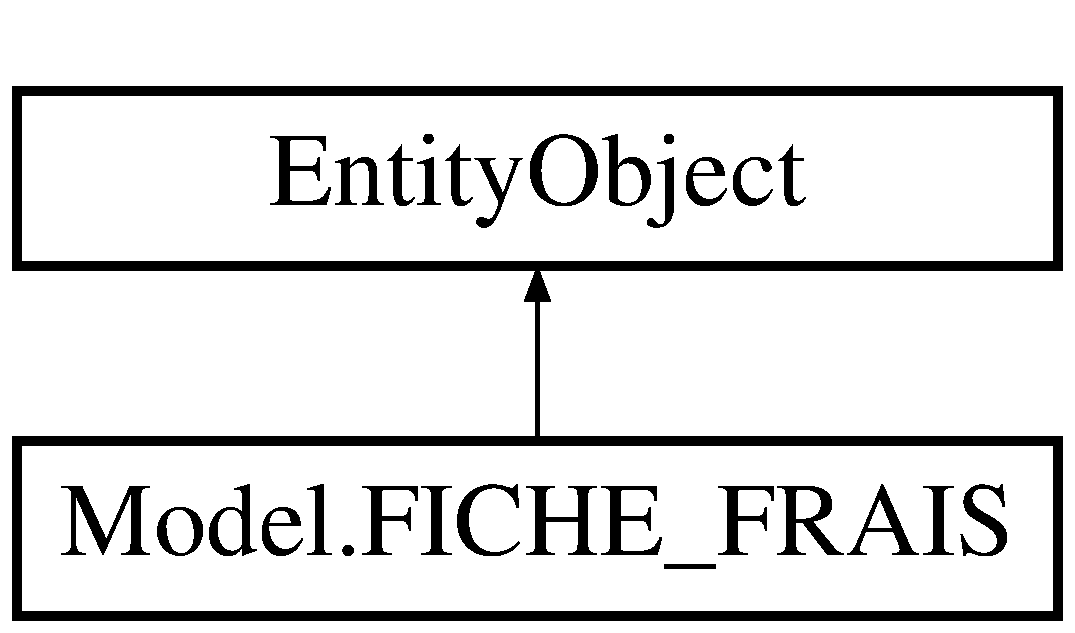
\includegraphics[height=2.000000cm]{class_model_1_1_f_i_c_h_e___f_r_a_i_s}
\end{center}
\end{figure}
\subsection*{Static Public Member Functions}
\begin{DoxyCompactItemize}
\item 
static \hyperlink{class_model_1_1_f_i_c_h_e___f_r_a_i_s}{F\-I\-C\-H\-E\-\_\-\-F\-R\-A\-I\-S} \hyperlink{class_model_1_1_f_i_c_h_e___f_r_a_i_s_a6498fb4372397a7caf9cdb0cf7f04985}{Create\-F\-I\-C\-H\-E\-\_\-\-F\-R\-A\-I\-S} (global\-::\-System.\-String \hyperlink{class_model_1_1_f_i_c_h_e___f_r_a_i_s_a5eb7f69b224a609736362ff9827a478c}{ff\-\_\-mois})
\begin{DoxyCompactList}\small\item\em Créez un nouvel objet \hyperlink{class_model_1_1_f_i_c_h_e___f_r_a_i_s}{F\-I\-C\-H\-E\-\_\-\-F\-R\-A\-I\-S}. \end{DoxyCompactList}\end{DoxyCompactItemize}
\subsection*{Properties}
\begin{DoxyCompactItemize}
\item 
global\-::\-System.\-String \hyperlink{class_model_1_1_f_i_c_h_e___f_r_a_i_s_a5eb7f69b224a609736362ff9827a478c}{ff\-\_\-mois}\hspace{0.3cm}{\ttfamily  \mbox{[}get, set\mbox{]}}
\begin{DoxyCompactList}\small\item\em Aucune documentation sur les métadonnées n'est disponible. \end{DoxyCompactList}\item 
Nullable$<$ global\-::\-System.\-Int32 $>$ \hyperlink{class_model_1_1_f_i_c_h_e___f_r_a_i_s_a57c78dba67ba315b60093f12a6b4687b}{matricule\-\_\-col\-\_\-fic}\hspace{0.3cm}{\ttfamily  \mbox{[}get, set\mbox{]}}
\begin{DoxyCompactList}\small\item\em Aucune documentation sur les métadonnées n'est disponible. \end{DoxyCompactList}\item 
global\-::\-System.\-String \hyperlink{class_model_1_1_f_i_c_h_e___f_r_a_i_s_ad5391808a353591c1469fa57668079d0}{ff\-\_\-\-N\-B\-Hors\-Classif}\hspace{0.3cm}{\ttfamily  \mbox{[}get, set\mbox{]}}
\begin{DoxyCompactList}\small\item\em Aucune documentation sur les métadonnées n'est disponible. \end{DoxyCompactList}\item 
global\-::\-System.\-String \hyperlink{class_model_1_1_f_i_c_h_e___f_r_a_i_s_af42dd6d52cf739434c1a9381c86f43f8}{ff\-\_\-\-Montant\-Hors\-Classif}\hspace{0.3cm}{\ttfamily  \mbox{[}get, set\mbox{]}}
\begin{DoxyCompactList}\small\item\em Aucune documentation sur les métadonnées n'est disponible. \end{DoxyCompactList}\item 
\hyperlink{class_model_1_1_c_o_l_l_a_b_o_r_a_t_e_u_r}{C\-O\-L\-L\-A\-B\-O\-R\-A\-T\-E\-U\-R} \hyperlink{class_model_1_1_f_i_c_h_e___f_r_a_i_s_a5026ccabe3b6b3c196a9d6a91dd1ef04}{C\-O\-L\-L\-A\-B\-O\-R\-A\-T\-E\-U\-R}\hspace{0.3cm}{\ttfamily  \mbox{[}get, set\mbox{]}}
\begin{DoxyCompactList}\small\item\em Aucune documentation sur les métadonnées n'est disponible. \end{DoxyCompactList}\item 
Entity\-Reference$<$ \hyperlink{class_model_1_1_c_o_l_l_a_b_o_r_a_t_e_u_r}{C\-O\-L\-L\-A\-B\-O\-R\-A\-T\-E\-U\-R} $>$ \hyperlink{class_model_1_1_f_i_c_h_e___f_r_a_i_s_ab0fd3a18afc02ce182fed71f9d4e385c}{C\-O\-L\-L\-A\-B\-O\-R\-A\-T\-E\-U\-R\-Reference}\hspace{0.3cm}{\ttfamily  \mbox{[}get, set\mbox{]}}
\begin{DoxyCompactList}\small\item\em Aucune documentation sur les métadonnées n'est disponible. \end{DoxyCompactList}\item 
Entity\-Collection$<$ \hyperlink{class_model_1_1_t_y_p_e___f_r_a_i_s}{T\-Y\-P\-E\-\_\-\-F\-R\-A\-I\-S} $>$ \hyperlink{class_model_1_1_f_i_c_h_e___f_r_a_i_s_ae41fdc6206cbf4c5cb2538bf8254f44b}{T\-Y\-P\-E\-\_\-\-F\-R\-A\-I\-S}\hspace{0.3cm}{\ttfamily  \mbox{[}get, set\mbox{]}}
\begin{DoxyCompactList}\small\item\em Aucune documentation sur les métadonnées n'est disponible. \end{DoxyCompactList}\end{DoxyCompactItemize}


\subsection{Detailed Description}
Aucune documentation sur les métadonnées n'est disponible. 



\subsection{Member Function Documentation}
\hypertarget{class_model_1_1_f_i_c_h_e___f_r_a_i_s_a6498fb4372397a7caf9cdb0cf7f04985}{\index{Model\-::\-F\-I\-C\-H\-E\-\_\-\-F\-R\-A\-I\-S@{Model\-::\-F\-I\-C\-H\-E\-\_\-\-F\-R\-A\-I\-S}!Create\-F\-I\-C\-H\-E\-\_\-\-F\-R\-A\-I\-S@{Create\-F\-I\-C\-H\-E\-\_\-\-F\-R\-A\-I\-S}}
\index{Create\-F\-I\-C\-H\-E\-\_\-\-F\-R\-A\-I\-S@{Create\-F\-I\-C\-H\-E\-\_\-\-F\-R\-A\-I\-S}!Model::FICHE_FRAIS@{Model\-::\-F\-I\-C\-H\-E\-\_\-\-F\-R\-A\-I\-S}}
\subsubsection[{Create\-F\-I\-C\-H\-E\-\_\-\-F\-R\-A\-I\-S}]{\setlength{\rightskip}{0pt plus 5cm}static {\bf F\-I\-C\-H\-E\-\_\-\-F\-R\-A\-I\-S} Model.\-F\-I\-C\-H\-E\-\_\-\-F\-R\-A\-I\-S.\-Create\-F\-I\-C\-H\-E\-\_\-\-F\-R\-A\-I\-S (
\begin{DoxyParamCaption}
\item[{global\-::\-System.\-String}]{ff\-\_\-mois}
\end{DoxyParamCaption}
)\hspace{0.3cm}{\ttfamily [static]}}}\label{class_model_1_1_f_i_c_h_e___f_r_a_i_s_a6498fb4372397a7caf9cdb0cf7f04985}


Créez un nouvel objet \hyperlink{class_model_1_1_f_i_c_h_e___f_r_a_i_s}{F\-I\-C\-H\-E\-\_\-\-F\-R\-A\-I\-S}. 


\begin{DoxyParams}{Parameters}
{\em ff\-\_\-mois} & Valeur initiale de la propriété ff\-\_\-mois.\\
\hline
\end{DoxyParams}


\subsection{Property Documentation}
\hypertarget{class_model_1_1_f_i_c_h_e___f_r_a_i_s_a5026ccabe3b6b3c196a9d6a91dd1ef04}{\index{Model\-::\-F\-I\-C\-H\-E\-\_\-\-F\-R\-A\-I\-S@{Model\-::\-F\-I\-C\-H\-E\-\_\-\-F\-R\-A\-I\-S}!C\-O\-L\-L\-A\-B\-O\-R\-A\-T\-E\-U\-R@{C\-O\-L\-L\-A\-B\-O\-R\-A\-T\-E\-U\-R}}
\index{C\-O\-L\-L\-A\-B\-O\-R\-A\-T\-E\-U\-R@{C\-O\-L\-L\-A\-B\-O\-R\-A\-T\-E\-U\-R}!Model::FICHE_FRAIS@{Model\-::\-F\-I\-C\-H\-E\-\_\-\-F\-R\-A\-I\-S}}
\subsubsection[{C\-O\-L\-L\-A\-B\-O\-R\-A\-T\-E\-U\-R}]{\setlength{\rightskip}{0pt plus 5cm}{\bf C\-O\-L\-L\-A\-B\-O\-R\-A\-T\-E\-U\-R} Model.\-F\-I\-C\-H\-E\-\_\-\-F\-R\-A\-I\-S.\-C\-O\-L\-L\-A\-B\-O\-R\-A\-T\-E\-U\-R\hspace{0.3cm}{\ttfamily [get]}, {\ttfamily [set]}}}\label{class_model_1_1_f_i_c_h_e___f_r_a_i_s_a5026ccabe3b6b3c196a9d6a91dd1ef04}


Aucune documentation sur les métadonnées n'est disponible. 

\hypertarget{class_model_1_1_f_i_c_h_e___f_r_a_i_s_ab0fd3a18afc02ce182fed71f9d4e385c}{\index{Model\-::\-F\-I\-C\-H\-E\-\_\-\-F\-R\-A\-I\-S@{Model\-::\-F\-I\-C\-H\-E\-\_\-\-F\-R\-A\-I\-S}!C\-O\-L\-L\-A\-B\-O\-R\-A\-T\-E\-U\-R\-Reference@{C\-O\-L\-L\-A\-B\-O\-R\-A\-T\-E\-U\-R\-Reference}}
\index{C\-O\-L\-L\-A\-B\-O\-R\-A\-T\-E\-U\-R\-Reference@{C\-O\-L\-L\-A\-B\-O\-R\-A\-T\-E\-U\-R\-Reference}!Model::FICHE_FRAIS@{Model\-::\-F\-I\-C\-H\-E\-\_\-\-F\-R\-A\-I\-S}}
\subsubsection[{C\-O\-L\-L\-A\-B\-O\-R\-A\-T\-E\-U\-R\-Reference}]{\setlength{\rightskip}{0pt plus 5cm}Entity\-Reference$<${\bf C\-O\-L\-L\-A\-B\-O\-R\-A\-T\-E\-U\-R}$>$ Model.\-F\-I\-C\-H\-E\-\_\-\-F\-R\-A\-I\-S.\-C\-O\-L\-L\-A\-B\-O\-R\-A\-T\-E\-U\-R\-Reference\hspace{0.3cm}{\ttfamily [get]}, {\ttfamily [set]}}}\label{class_model_1_1_f_i_c_h_e___f_r_a_i_s_ab0fd3a18afc02ce182fed71f9d4e385c}


Aucune documentation sur les métadonnées n'est disponible. 

\hypertarget{class_model_1_1_f_i_c_h_e___f_r_a_i_s_a5eb7f69b224a609736362ff9827a478c}{\index{Model\-::\-F\-I\-C\-H\-E\-\_\-\-F\-R\-A\-I\-S@{Model\-::\-F\-I\-C\-H\-E\-\_\-\-F\-R\-A\-I\-S}!ff\-\_\-mois@{ff\-\_\-mois}}
\index{ff\-\_\-mois@{ff\-\_\-mois}!Model::FICHE_FRAIS@{Model\-::\-F\-I\-C\-H\-E\-\_\-\-F\-R\-A\-I\-S}}
\subsubsection[{ff\-\_\-mois}]{\setlength{\rightskip}{0pt plus 5cm}global.\-System.\-String Model.\-F\-I\-C\-H\-E\-\_\-\-F\-R\-A\-I\-S.\-ff\-\_\-mois\hspace{0.3cm}{\ttfamily [get]}, {\ttfamily [set]}}}\label{class_model_1_1_f_i_c_h_e___f_r_a_i_s_a5eb7f69b224a609736362ff9827a478c}


Aucune documentation sur les métadonnées n'est disponible. 

\hypertarget{class_model_1_1_f_i_c_h_e___f_r_a_i_s_af42dd6d52cf739434c1a9381c86f43f8}{\index{Model\-::\-F\-I\-C\-H\-E\-\_\-\-F\-R\-A\-I\-S@{Model\-::\-F\-I\-C\-H\-E\-\_\-\-F\-R\-A\-I\-S}!ff\-\_\-\-Montant\-Hors\-Classif@{ff\-\_\-\-Montant\-Hors\-Classif}}
\index{ff\-\_\-\-Montant\-Hors\-Classif@{ff\-\_\-\-Montant\-Hors\-Classif}!Model::FICHE_FRAIS@{Model\-::\-F\-I\-C\-H\-E\-\_\-\-F\-R\-A\-I\-S}}
\subsubsection[{ff\-\_\-\-Montant\-Hors\-Classif}]{\setlength{\rightskip}{0pt plus 5cm}global.\-System.\-String Model.\-F\-I\-C\-H\-E\-\_\-\-F\-R\-A\-I\-S.\-ff\-\_\-\-Montant\-Hors\-Classif\hspace{0.3cm}{\ttfamily [get]}, {\ttfamily [set]}}}\label{class_model_1_1_f_i_c_h_e___f_r_a_i_s_af42dd6d52cf739434c1a9381c86f43f8}


Aucune documentation sur les métadonnées n'est disponible. 

\hypertarget{class_model_1_1_f_i_c_h_e___f_r_a_i_s_ad5391808a353591c1469fa57668079d0}{\index{Model\-::\-F\-I\-C\-H\-E\-\_\-\-F\-R\-A\-I\-S@{Model\-::\-F\-I\-C\-H\-E\-\_\-\-F\-R\-A\-I\-S}!ff\-\_\-\-N\-B\-Hors\-Classif@{ff\-\_\-\-N\-B\-Hors\-Classif}}
\index{ff\-\_\-\-N\-B\-Hors\-Classif@{ff\-\_\-\-N\-B\-Hors\-Classif}!Model::FICHE_FRAIS@{Model\-::\-F\-I\-C\-H\-E\-\_\-\-F\-R\-A\-I\-S}}
\subsubsection[{ff\-\_\-\-N\-B\-Hors\-Classif}]{\setlength{\rightskip}{0pt plus 5cm}global.\-System.\-String Model.\-F\-I\-C\-H\-E\-\_\-\-F\-R\-A\-I\-S.\-ff\-\_\-\-N\-B\-Hors\-Classif\hspace{0.3cm}{\ttfamily [get]}, {\ttfamily [set]}}}\label{class_model_1_1_f_i_c_h_e___f_r_a_i_s_ad5391808a353591c1469fa57668079d0}


Aucune documentation sur les métadonnées n'est disponible. 

\hypertarget{class_model_1_1_f_i_c_h_e___f_r_a_i_s_a57c78dba67ba315b60093f12a6b4687b}{\index{Model\-::\-F\-I\-C\-H\-E\-\_\-\-F\-R\-A\-I\-S@{Model\-::\-F\-I\-C\-H\-E\-\_\-\-F\-R\-A\-I\-S}!matricule\-\_\-col\-\_\-fic@{matricule\-\_\-col\-\_\-fic}}
\index{matricule\-\_\-col\-\_\-fic@{matricule\-\_\-col\-\_\-fic}!Model::FICHE_FRAIS@{Model\-::\-F\-I\-C\-H\-E\-\_\-\-F\-R\-A\-I\-S}}
\subsubsection[{matricule\-\_\-col\-\_\-fic}]{\setlength{\rightskip}{0pt plus 5cm}Nullable$<$global.\-System.\-Int32$>$ Model.\-F\-I\-C\-H\-E\-\_\-\-F\-R\-A\-I\-S.\-matricule\-\_\-col\-\_\-fic\hspace{0.3cm}{\ttfamily [get]}, {\ttfamily [set]}}}\label{class_model_1_1_f_i_c_h_e___f_r_a_i_s_a57c78dba67ba315b60093f12a6b4687b}


Aucune documentation sur les métadonnées n'est disponible. 

\hypertarget{class_model_1_1_f_i_c_h_e___f_r_a_i_s_ae41fdc6206cbf4c5cb2538bf8254f44b}{\index{Model\-::\-F\-I\-C\-H\-E\-\_\-\-F\-R\-A\-I\-S@{Model\-::\-F\-I\-C\-H\-E\-\_\-\-F\-R\-A\-I\-S}!T\-Y\-P\-E\-\_\-\-F\-R\-A\-I\-S@{T\-Y\-P\-E\-\_\-\-F\-R\-A\-I\-S}}
\index{T\-Y\-P\-E\-\_\-\-F\-R\-A\-I\-S@{T\-Y\-P\-E\-\_\-\-F\-R\-A\-I\-S}!Model::FICHE_FRAIS@{Model\-::\-F\-I\-C\-H\-E\-\_\-\-F\-R\-A\-I\-S}}
\subsubsection[{T\-Y\-P\-E\-\_\-\-F\-R\-A\-I\-S}]{\setlength{\rightskip}{0pt plus 5cm}Entity\-Collection$<${\bf T\-Y\-P\-E\-\_\-\-F\-R\-A\-I\-S}$>$ Model.\-F\-I\-C\-H\-E\-\_\-\-F\-R\-A\-I\-S.\-T\-Y\-P\-E\-\_\-\-F\-R\-A\-I\-S\hspace{0.3cm}{\ttfamily [get]}, {\ttfamily [set]}}}\label{class_model_1_1_f_i_c_h_e___f_r_a_i_s_ae41fdc6206cbf4c5cb2538bf8254f44b}


Aucune documentation sur les métadonnées n'est disponible. 



The documentation for this class was generated from the following file\-:\begin{DoxyCompactItemize}
\item 
C\-:/\-Users/dju/\-Documents/\-Visual Studio 2012/\-Projects/\-P\-P\-E/\-P\-P\-E3/\-Model/\hyperlink{_model_bdd_sio_8_designer_8cs}{Model\-Bdd\-Sio.\-Designer.\-cs}\end{DoxyCompactItemize}

\hypertarget{struct_wpf_application_1_1_view_model_1_1_filtre_struct}{\section{Wpf\-Application.\-View\-Model.\-Filtre\-Struct Struct Reference}
\label{struct_wpf_application_1_1_view_model_1_1_filtre_struct}\index{Wpf\-Application.\-View\-Model.\-Filtre\-Struct@{Wpf\-Application.\-View\-Model.\-Filtre\-Struct}}
}
\subsection*{Properties}
\begin{DoxyCompactItemize}
\item 
string \hyperlink{struct_wpf_application_1_1_view_model_1_1_filtre_struct_a8a2947c536dcde711e38237e559e7e7f}{Valeur}\hspace{0.3cm}{\ttfamily  \mbox{[}get, set\mbox{]}}
\item 
string \hyperlink{struct_wpf_application_1_1_view_model_1_1_filtre_struct_a4f5123d8dd012d39c85fe96b4c135cd8}{Champ}\hspace{0.3cm}{\ttfamily  \mbox{[}get, set\mbox{]}}
\end{DoxyCompactItemize}


\subsection{Property Documentation}
\hypertarget{struct_wpf_application_1_1_view_model_1_1_filtre_struct_a4f5123d8dd012d39c85fe96b4c135cd8}{\index{Wpf\-Application\-::\-View\-Model\-::\-Filtre\-Struct@{Wpf\-Application\-::\-View\-Model\-::\-Filtre\-Struct}!Champ@{Champ}}
\index{Champ@{Champ}!WpfApplication::ViewModel::FiltreStruct@{Wpf\-Application\-::\-View\-Model\-::\-Filtre\-Struct}}
\subsubsection[{Champ}]{\setlength{\rightskip}{0pt plus 5cm}string Wpf\-Application.\-View\-Model.\-Filtre\-Struct.\-Champ\hspace{0.3cm}{\ttfamily [get]}, {\ttfamily [set]}}}\label{struct_wpf_application_1_1_view_model_1_1_filtre_struct_a4f5123d8dd012d39c85fe96b4c135cd8}
\hypertarget{struct_wpf_application_1_1_view_model_1_1_filtre_struct_a8a2947c536dcde711e38237e559e7e7f}{\index{Wpf\-Application\-::\-View\-Model\-::\-Filtre\-Struct@{Wpf\-Application\-::\-View\-Model\-::\-Filtre\-Struct}!Valeur@{Valeur}}
\index{Valeur@{Valeur}!WpfApplication::ViewModel::FiltreStruct@{Wpf\-Application\-::\-View\-Model\-::\-Filtre\-Struct}}
\subsubsection[{Valeur}]{\setlength{\rightskip}{0pt plus 5cm}string Wpf\-Application.\-View\-Model.\-Filtre\-Struct.\-Valeur\hspace{0.3cm}{\ttfamily [get]}, {\ttfamily [set]}}}\label{struct_wpf_application_1_1_view_model_1_1_filtre_struct_a8a2947c536dcde711e38237e559e7e7f}


The documentation for this struct was generated from the following file\-:\begin{DoxyCompactItemize}
\item 
C\-:/\-Users/dju/\-Documents/\-Visual Studio 2012/\-Projects/\-P\-P\-E/\-P\-P\-E3/\-Wpf\-Application/\-View\-Model/\hyperlink{_main_window_view_model_8cs}{Main\-Window\-View\-Model.\-cs}\end{DoxyCompactItemize}

\hypertarget{class_xaml_generated_namespace_1_1_generated_internal_type_helper}{\section{Xaml\-Generated\-Namespace.\-Generated\-Internal\-Type\-Helper Class Reference}
\label{class_xaml_generated_namespace_1_1_generated_internal_type_helper}\index{Xaml\-Generated\-Namespace.\-Generated\-Internal\-Type\-Helper@{Xaml\-Generated\-Namespace.\-Generated\-Internal\-Type\-Helper}}
}


\hyperlink{class_xaml_generated_namespace_1_1_generated_internal_type_helper}{Generated\-Internal\-Type\-Helper}  


Inheritance diagram for Xaml\-Generated\-Namespace.\-Generated\-Internal\-Type\-Helper\-:\begin{figure}[H]
\begin{center}
\leavevmode
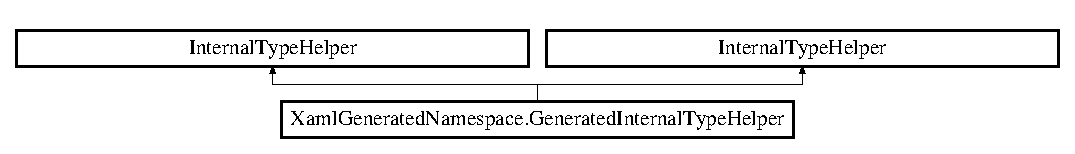
\includegraphics[height=1.627907cm]{class_xaml_generated_namespace_1_1_generated_internal_type_helper}
\end{center}
\end{figure}
\subsection*{Protected Member Functions}
\begin{DoxyCompactItemize}
\item 
override object \hyperlink{class_xaml_generated_namespace_1_1_generated_internal_type_helper_aefb7a98fceb9c287cef4756942f441d1}{Create\-Instance} (System.\-Type type, System.\-Globalization.\-Culture\-Info culture)
\begin{DoxyCompactList}\small\item\em Create\-Instance \end{DoxyCompactList}\item 
override object \hyperlink{class_xaml_generated_namespace_1_1_generated_internal_type_helper_afdc9fe15b56607d02082908d934480c6}{Get\-Property\-Value} (System.\-Reflection.\-Property\-Info property\-Info, object target, System.\-Globalization.\-Culture\-Info culture)
\begin{DoxyCompactList}\small\item\em Get\-Property\-Value \end{DoxyCompactList}\item 
override void \hyperlink{class_xaml_generated_namespace_1_1_generated_internal_type_helper_ade0f04c0f7b18dd5b170e071d5534d38}{Set\-Property\-Value} (System.\-Reflection.\-Property\-Info property\-Info, object target, object value, System.\-Globalization.\-Culture\-Info culture)
\begin{DoxyCompactList}\small\item\em Set\-Property\-Value \end{DoxyCompactList}\item 
override System.\-Delegate \hyperlink{class_xaml_generated_namespace_1_1_generated_internal_type_helper_a8ec4c37e82d9f4e867e9655f4eac3a78}{Create\-Delegate} (System.\-Type delegate\-Type, object target, string handler)
\begin{DoxyCompactList}\small\item\em Create\-Delegate \end{DoxyCompactList}\item 
override void \hyperlink{class_xaml_generated_namespace_1_1_generated_internal_type_helper_a73471f4a6d1ca4c4fceec9ad8610f0c8}{Add\-Event\-Handler} (System.\-Reflection.\-Event\-Info event\-Info, object target, System.\-Delegate handler)
\begin{DoxyCompactList}\small\item\em Add\-Event\-Handler \end{DoxyCompactList}\item 
override object \hyperlink{class_xaml_generated_namespace_1_1_generated_internal_type_helper_aefb7a98fceb9c287cef4756942f441d1}{Create\-Instance} (System.\-Type type, System.\-Globalization.\-Culture\-Info culture)
\begin{DoxyCompactList}\small\item\em Create\-Instance \end{DoxyCompactList}\item 
override object \hyperlink{class_xaml_generated_namespace_1_1_generated_internal_type_helper_afdc9fe15b56607d02082908d934480c6}{Get\-Property\-Value} (System.\-Reflection.\-Property\-Info property\-Info, object target, System.\-Globalization.\-Culture\-Info culture)
\begin{DoxyCompactList}\small\item\em Get\-Property\-Value \end{DoxyCompactList}\item 
override void \hyperlink{class_xaml_generated_namespace_1_1_generated_internal_type_helper_ade0f04c0f7b18dd5b170e071d5534d38}{Set\-Property\-Value} (System.\-Reflection.\-Property\-Info property\-Info, object target, object value, System.\-Globalization.\-Culture\-Info culture)
\begin{DoxyCompactList}\small\item\em Set\-Property\-Value \end{DoxyCompactList}\item 
override System.\-Delegate \hyperlink{class_xaml_generated_namespace_1_1_generated_internal_type_helper_a8ec4c37e82d9f4e867e9655f4eac3a78}{Create\-Delegate} (System.\-Type delegate\-Type, object target, string handler)
\begin{DoxyCompactList}\small\item\em Create\-Delegate \end{DoxyCompactList}\item 
override void \hyperlink{class_xaml_generated_namespace_1_1_generated_internal_type_helper_a73471f4a6d1ca4c4fceec9ad8610f0c8}{Add\-Event\-Handler} (System.\-Reflection.\-Event\-Info event\-Info, object target, System.\-Delegate handler)
\begin{DoxyCompactList}\small\item\em Add\-Event\-Handler \end{DoxyCompactList}\end{DoxyCompactItemize}


\subsection{Detailed Description}
\hyperlink{class_xaml_generated_namespace_1_1_generated_internal_type_helper}{Generated\-Internal\-Type\-Helper} 



\subsection{Member Function Documentation}
\hypertarget{class_xaml_generated_namespace_1_1_generated_internal_type_helper_a73471f4a6d1ca4c4fceec9ad8610f0c8}{\index{Xaml\-Generated\-Namespace\-::\-Generated\-Internal\-Type\-Helper@{Xaml\-Generated\-Namespace\-::\-Generated\-Internal\-Type\-Helper}!Add\-Event\-Handler@{Add\-Event\-Handler}}
\index{Add\-Event\-Handler@{Add\-Event\-Handler}!XamlGeneratedNamespace::GeneratedInternalTypeHelper@{Xaml\-Generated\-Namespace\-::\-Generated\-Internal\-Type\-Helper}}
\subsubsection[{Add\-Event\-Handler}]{\setlength{\rightskip}{0pt plus 5cm}override void Xaml\-Generated\-Namespace.\-Generated\-Internal\-Type\-Helper.\-Add\-Event\-Handler (
\begin{DoxyParamCaption}
\item[{System.\-Reflection.\-Event\-Info}]{event\-Info, }
\item[{object}]{target, }
\item[{System.\-Delegate}]{handler}
\end{DoxyParamCaption}
)\hspace{0.3cm}{\ttfamily [protected]}}}\label{class_xaml_generated_namespace_1_1_generated_internal_type_helper_a73471f4a6d1ca4c4fceec9ad8610f0c8}


Add\-Event\-Handler 

\hypertarget{class_xaml_generated_namespace_1_1_generated_internal_type_helper_a73471f4a6d1ca4c4fceec9ad8610f0c8}{\index{Xaml\-Generated\-Namespace\-::\-Generated\-Internal\-Type\-Helper@{Xaml\-Generated\-Namespace\-::\-Generated\-Internal\-Type\-Helper}!Add\-Event\-Handler@{Add\-Event\-Handler}}
\index{Add\-Event\-Handler@{Add\-Event\-Handler}!XamlGeneratedNamespace::GeneratedInternalTypeHelper@{Xaml\-Generated\-Namespace\-::\-Generated\-Internal\-Type\-Helper}}
\subsubsection[{Add\-Event\-Handler}]{\setlength{\rightskip}{0pt plus 5cm}override void Xaml\-Generated\-Namespace.\-Generated\-Internal\-Type\-Helper.\-Add\-Event\-Handler (
\begin{DoxyParamCaption}
\item[{System.\-Reflection.\-Event\-Info}]{event\-Info, }
\item[{object}]{target, }
\item[{System.\-Delegate}]{handler}
\end{DoxyParamCaption}
)\hspace{0.3cm}{\ttfamily [protected]}}}\label{class_xaml_generated_namespace_1_1_generated_internal_type_helper_a73471f4a6d1ca4c4fceec9ad8610f0c8}


Add\-Event\-Handler 

\hypertarget{class_xaml_generated_namespace_1_1_generated_internal_type_helper_a8ec4c37e82d9f4e867e9655f4eac3a78}{\index{Xaml\-Generated\-Namespace\-::\-Generated\-Internal\-Type\-Helper@{Xaml\-Generated\-Namespace\-::\-Generated\-Internal\-Type\-Helper}!Create\-Delegate@{Create\-Delegate}}
\index{Create\-Delegate@{Create\-Delegate}!XamlGeneratedNamespace::GeneratedInternalTypeHelper@{Xaml\-Generated\-Namespace\-::\-Generated\-Internal\-Type\-Helper}}
\subsubsection[{Create\-Delegate}]{\setlength{\rightskip}{0pt plus 5cm}override System.\-Delegate Xaml\-Generated\-Namespace.\-Generated\-Internal\-Type\-Helper.\-Create\-Delegate (
\begin{DoxyParamCaption}
\item[{System.\-Type}]{delegate\-Type, }
\item[{object}]{target, }
\item[{string}]{handler}
\end{DoxyParamCaption}
)\hspace{0.3cm}{\ttfamily [protected]}}}\label{class_xaml_generated_namespace_1_1_generated_internal_type_helper_a8ec4c37e82d9f4e867e9655f4eac3a78}


Create\-Delegate 

\hypertarget{class_xaml_generated_namespace_1_1_generated_internal_type_helper_a8ec4c37e82d9f4e867e9655f4eac3a78}{\index{Xaml\-Generated\-Namespace\-::\-Generated\-Internal\-Type\-Helper@{Xaml\-Generated\-Namespace\-::\-Generated\-Internal\-Type\-Helper}!Create\-Delegate@{Create\-Delegate}}
\index{Create\-Delegate@{Create\-Delegate}!XamlGeneratedNamespace::GeneratedInternalTypeHelper@{Xaml\-Generated\-Namespace\-::\-Generated\-Internal\-Type\-Helper}}
\subsubsection[{Create\-Delegate}]{\setlength{\rightskip}{0pt plus 5cm}override System.\-Delegate Xaml\-Generated\-Namespace.\-Generated\-Internal\-Type\-Helper.\-Create\-Delegate (
\begin{DoxyParamCaption}
\item[{System.\-Type}]{delegate\-Type, }
\item[{object}]{target, }
\item[{string}]{handler}
\end{DoxyParamCaption}
)\hspace{0.3cm}{\ttfamily [protected]}}}\label{class_xaml_generated_namespace_1_1_generated_internal_type_helper_a8ec4c37e82d9f4e867e9655f4eac3a78}


Create\-Delegate 

\hypertarget{class_xaml_generated_namespace_1_1_generated_internal_type_helper_aefb7a98fceb9c287cef4756942f441d1}{\index{Xaml\-Generated\-Namespace\-::\-Generated\-Internal\-Type\-Helper@{Xaml\-Generated\-Namespace\-::\-Generated\-Internal\-Type\-Helper}!Create\-Instance@{Create\-Instance}}
\index{Create\-Instance@{Create\-Instance}!XamlGeneratedNamespace::GeneratedInternalTypeHelper@{Xaml\-Generated\-Namespace\-::\-Generated\-Internal\-Type\-Helper}}
\subsubsection[{Create\-Instance}]{\setlength{\rightskip}{0pt plus 5cm}override object Xaml\-Generated\-Namespace.\-Generated\-Internal\-Type\-Helper.\-Create\-Instance (
\begin{DoxyParamCaption}
\item[{System.\-Type}]{type, }
\item[{System.\-Globalization.\-Culture\-Info}]{culture}
\end{DoxyParamCaption}
)\hspace{0.3cm}{\ttfamily [protected]}}}\label{class_xaml_generated_namespace_1_1_generated_internal_type_helper_aefb7a98fceb9c287cef4756942f441d1}


Create\-Instance 

\hypertarget{class_xaml_generated_namespace_1_1_generated_internal_type_helper_aefb7a98fceb9c287cef4756942f441d1}{\index{Xaml\-Generated\-Namespace\-::\-Generated\-Internal\-Type\-Helper@{Xaml\-Generated\-Namespace\-::\-Generated\-Internal\-Type\-Helper}!Create\-Instance@{Create\-Instance}}
\index{Create\-Instance@{Create\-Instance}!XamlGeneratedNamespace::GeneratedInternalTypeHelper@{Xaml\-Generated\-Namespace\-::\-Generated\-Internal\-Type\-Helper}}
\subsubsection[{Create\-Instance}]{\setlength{\rightskip}{0pt plus 5cm}override object Xaml\-Generated\-Namespace.\-Generated\-Internal\-Type\-Helper.\-Create\-Instance (
\begin{DoxyParamCaption}
\item[{System.\-Type}]{type, }
\item[{System.\-Globalization.\-Culture\-Info}]{culture}
\end{DoxyParamCaption}
)\hspace{0.3cm}{\ttfamily [protected]}}}\label{class_xaml_generated_namespace_1_1_generated_internal_type_helper_aefb7a98fceb9c287cef4756942f441d1}


Create\-Instance 

\hypertarget{class_xaml_generated_namespace_1_1_generated_internal_type_helper_afdc9fe15b56607d02082908d934480c6}{\index{Xaml\-Generated\-Namespace\-::\-Generated\-Internal\-Type\-Helper@{Xaml\-Generated\-Namespace\-::\-Generated\-Internal\-Type\-Helper}!Get\-Property\-Value@{Get\-Property\-Value}}
\index{Get\-Property\-Value@{Get\-Property\-Value}!XamlGeneratedNamespace::GeneratedInternalTypeHelper@{Xaml\-Generated\-Namespace\-::\-Generated\-Internal\-Type\-Helper}}
\subsubsection[{Get\-Property\-Value}]{\setlength{\rightskip}{0pt plus 5cm}override object Xaml\-Generated\-Namespace.\-Generated\-Internal\-Type\-Helper.\-Get\-Property\-Value (
\begin{DoxyParamCaption}
\item[{System.\-Reflection.\-Property\-Info}]{property\-Info, }
\item[{object}]{target, }
\item[{System.\-Globalization.\-Culture\-Info}]{culture}
\end{DoxyParamCaption}
)\hspace{0.3cm}{\ttfamily [protected]}}}\label{class_xaml_generated_namespace_1_1_generated_internal_type_helper_afdc9fe15b56607d02082908d934480c6}


Get\-Property\-Value 

\hypertarget{class_xaml_generated_namespace_1_1_generated_internal_type_helper_afdc9fe15b56607d02082908d934480c6}{\index{Xaml\-Generated\-Namespace\-::\-Generated\-Internal\-Type\-Helper@{Xaml\-Generated\-Namespace\-::\-Generated\-Internal\-Type\-Helper}!Get\-Property\-Value@{Get\-Property\-Value}}
\index{Get\-Property\-Value@{Get\-Property\-Value}!XamlGeneratedNamespace::GeneratedInternalTypeHelper@{Xaml\-Generated\-Namespace\-::\-Generated\-Internal\-Type\-Helper}}
\subsubsection[{Get\-Property\-Value}]{\setlength{\rightskip}{0pt plus 5cm}override object Xaml\-Generated\-Namespace.\-Generated\-Internal\-Type\-Helper.\-Get\-Property\-Value (
\begin{DoxyParamCaption}
\item[{System.\-Reflection.\-Property\-Info}]{property\-Info, }
\item[{object}]{target, }
\item[{System.\-Globalization.\-Culture\-Info}]{culture}
\end{DoxyParamCaption}
)\hspace{0.3cm}{\ttfamily [protected]}}}\label{class_xaml_generated_namespace_1_1_generated_internal_type_helper_afdc9fe15b56607d02082908d934480c6}


Get\-Property\-Value 

\hypertarget{class_xaml_generated_namespace_1_1_generated_internal_type_helper_ade0f04c0f7b18dd5b170e071d5534d38}{\index{Xaml\-Generated\-Namespace\-::\-Generated\-Internal\-Type\-Helper@{Xaml\-Generated\-Namespace\-::\-Generated\-Internal\-Type\-Helper}!Set\-Property\-Value@{Set\-Property\-Value}}
\index{Set\-Property\-Value@{Set\-Property\-Value}!XamlGeneratedNamespace::GeneratedInternalTypeHelper@{Xaml\-Generated\-Namespace\-::\-Generated\-Internal\-Type\-Helper}}
\subsubsection[{Set\-Property\-Value}]{\setlength{\rightskip}{0pt plus 5cm}override void Xaml\-Generated\-Namespace.\-Generated\-Internal\-Type\-Helper.\-Set\-Property\-Value (
\begin{DoxyParamCaption}
\item[{System.\-Reflection.\-Property\-Info}]{property\-Info, }
\item[{object}]{target, }
\item[{object}]{value, }
\item[{System.\-Globalization.\-Culture\-Info}]{culture}
\end{DoxyParamCaption}
)\hspace{0.3cm}{\ttfamily [protected]}}}\label{class_xaml_generated_namespace_1_1_generated_internal_type_helper_ade0f04c0f7b18dd5b170e071d5534d38}


Set\-Property\-Value 

\hypertarget{class_xaml_generated_namespace_1_1_generated_internal_type_helper_ade0f04c0f7b18dd5b170e071d5534d38}{\index{Xaml\-Generated\-Namespace\-::\-Generated\-Internal\-Type\-Helper@{Xaml\-Generated\-Namespace\-::\-Generated\-Internal\-Type\-Helper}!Set\-Property\-Value@{Set\-Property\-Value}}
\index{Set\-Property\-Value@{Set\-Property\-Value}!XamlGeneratedNamespace::GeneratedInternalTypeHelper@{Xaml\-Generated\-Namespace\-::\-Generated\-Internal\-Type\-Helper}}
\subsubsection[{Set\-Property\-Value}]{\setlength{\rightskip}{0pt plus 5cm}override void Xaml\-Generated\-Namespace.\-Generated\-Internal\-Type\-Helper.\-Set\-Property\-Value (
\begin{DoxyParamCaption}
\item[{System.\-Reflection.\-Property\-Info}]{property\-Info, }
\item[{object}]{target, }
\item[{object}]{value, }
\item[{System.\-Globalization.\-Culture\-Info}]{culture}
\end{DoxyParamCaption}
)\hspace{0.3cm}{\ttfamily [protected]}}}\label{class_xaml_generated_namespace_1_1_generated_internal_type_helper_ade0f04c0f7b18dd5b170e071d5534d38}


Set\-Property\-Value 



The documentation for this class was generated from the following files\-:\begin{DoxyCompactItemize}
\item 
C\-:/\-Users/dju/\-Documents/\-Visual Studio 2012/\-Projects/\-P\-P\-E/\-P\-P\-E3/\-Wpf\-Application/obj/\-Debug/\hyperlink{_generated_internal_type_helper_8g_8cs}{Generated\-Internal\-Type\-Helper.\-g.\-cs}\item 
C\-:/\-Users/dju/\-Documents/\-Visual Studio 2012/\-Projects/\-P\-P\-E/\-P\-P\-E3/\-Wpf\-Application/obj/\-Debug/\hyperlink{_generated_internal_type_helper_8g_8i_8cs}{Generated\-Internal\-Type\-Helper.\-g.\-i.\-cs}\end{DoxyCompactItemize}

\hypertarget{class_model_1_1_g_e_r_e}{\section{Model.\-G\-E\-R\-E Class Reference}
\label{class_model_1_1_g_e_r_e}\index{Model.\-G\-E\-R\-E@{Model.\-G\-E\-R\-E}}
}


Aucune documentation sur les métadonnées n'est disponible.  


Inheritance diagram for Model.\-G\-E\-R\-E\-:\begin{figure}[H]
\begin{center}
\leavevmode
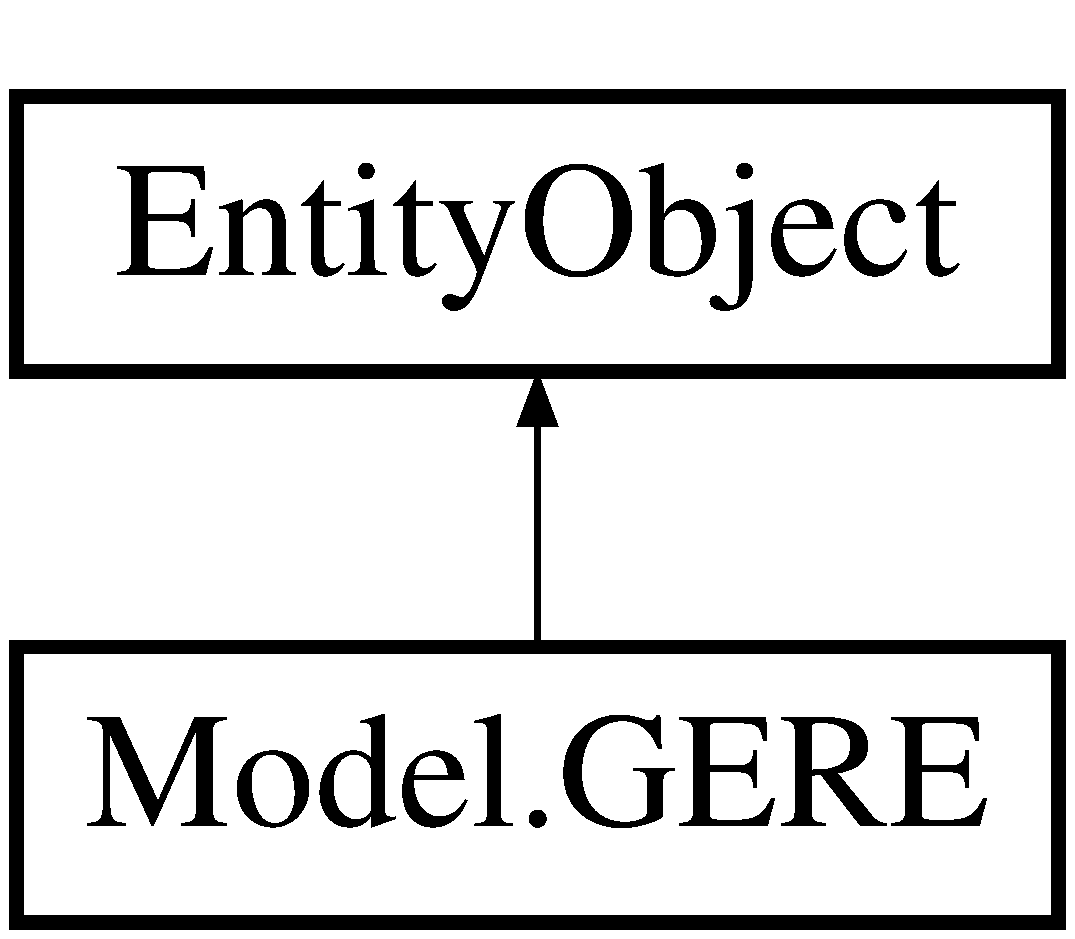
\includegraphics[height=2.000000cm]{class_model_1_1_g_e_r_e}
\end{center}
\end{figure}
\subsection*{Static Public Member Functions}
\begin{DoxyCompactItemize}
\item 
static \hyperlink{class_model_1_1_g_e_r_e}{G\-E\-R\-E} \hyperlink{class_model_1_1_g_e_r_e_a08f4c410666eaa384a4df6c5af56caeb}{Create\-G\-E\-R\-E} (global\-::\-System.\-Int32 \hyperlink{class_model_1_1_g_e_r_e_a6976ff90929344b89d6329df4f8b7648}{matricule\-\_\-col\-\_\-ger}, global\-::\-System.\-String \hyperlink{class_model_1_1_g_e_r_e_ab75ef8c99d225e8c5e4cf95012d54287}{code\-\_\-region}, global\-::\-System.\-Date\-Time j\-J\-M\-M\-A\-A\-A\-A\-\_\-\-F\-I\-N, global\-::\-System.\-Date\-Time j\-J\-M\-M\-A\-A\-A\-A\-\_\-\-D\-E\-B)
\begin{DoxyCompactList}\small\item\em Créez un nouvel objet \hyperlink{class_model_1_1_g_e_r_e}{G\-E\-R\-E}. \end{DoxyCompactList}\end{DoxyCompactItemize}
\subsection*{Properties}
\begin{DoxyCompactItemize}
\item 
global\-::\-System.\-Int32 \hyperlink{class_model_1_1_g_e_r_e_a6976ff90929344b89d6329df4f8b7648}{matricule\-\_\-col\-\_\-ger}\hspace{0.3cm}{\ttfamily  \mbox{[}get, set\mbox{]}}
\begin{DoxyCompactList}\small\item\em Aucune documentation sur les métadonnées n'est disponible. \end{DoxyCompactList}\item 
global\-::\-System.\-String \hyperlink{class_model_1_1_g_e_r_e_ab75ef8c99d225e8c5e4cf95012d54287}{code\-\_\-region}\hspace{0.3cm}{\ttfamily  \mbox{[}get, set\mbox{]}}
\begin{DoxyCompactList}\small\item\em Aucune documentation sur les métadonnées n'est disponible. \end{DoxyCompactList}\item 
global\-::\-System.\-Date\-Time \hyperlink{class_model_1_1_g_e_r_e_ad81d5bfe8fda3ba990d89ed4f31c282f}{J\-J\-M\-M\-A\-A\-A\-A\-\_\-\-F\-I\-N}\hspace{0.3cm}{\ttfamily  \mbox{[}get, set\mbox{]}}
\begin{DoxyCompactList}\small\item\em Aucune documentation sur les métadonnées n'est disponible. \end{DoxyCompactList}\item 
global\-::\-System.\-Date\-Time \hyperlink{class_model_1_1_g_e_r_e_a958847177a345b8807e3f3a5a0e7723e}{J\-J\-M\-M\-A\-A\-A\-A\-\_\-\-D\-E\-B}\hspace{0.3cm}{\ttfamily  \mbox{[}get, set\mbox{]}}
\begin{DoxyCompactList}\small\item\em Aucune documentation sur les métadonnées n'est disponible. \end{DoxyCompactList}\item 
\hyperlink{class_model_1_1_c_a_l_e_n_d_r_i_e_r}{C\-A\-L\-E\-N\-D\-R\-I\-E\-R} \hyperlink{class_model_1_1_g_e_r_e_a449b547ec0dae7611bdb626f4a712c2e}{C\-A\-L\-E\-N\-D\-R\-I\-E\-R}\hspace{0.3cm}{\ttfamily  \mbox{[}get, set\mbox{]}}
\begin{DoxyCompactList}\small\item\em Aucune documentation sur les métadonnées n'est disponible. \end{DoxyCompactList}\item 
Entity\-Reference$<$ \hyperlink{class_model_1_1_c_a_l_e_n_d_r_i_e_r}{C\-A\-L\-E\-N\-D\-R\-I\-E\-R} $>$ \hyperlink{class_model_1_1_g_e_r_e_a480b3df645ec158a0f1072ed6863e5e7}{C\-A\-L\-E\-N\-D\-R\-I\-E\-R\-Reference}\hspace{0.3cm}{\ttfamily  \mbox{[}get, set\mbox{]}}
\begin{DoxyCompactList}\small\item\em Aucune documentation sur les métadonnées n'est disponible. \end{DoxyCompactList}\item 
\hyperlink{class_model_1_1_c_o_l_l_a_b_o_r_a_t_e_u_r}{C\-O\-L\-L\-A\-B\-O\-R\-A\-T\-E\-U\-R} \hyperlink{class_model_1_1_g_e_r_e_a8a670e1a6e5780b22b61677e850fa913}{C\-O\-L\-L\-A\-B\-O\-R\-A\-T\-E\-U\-R}\hspace{0.3cm}{\ttfamily  \mbox{[}get, set\mbox{]}}
\begin{DoxyCompactList}\small\item\em Aucune documentation sur les métadonnées n'est disponible. \end{DoxyCompactList}\item 
Entity\-Reference$<$ \hyperlink{class_model_1_1_c_o_l_l_a_b_o_r_a_t_e_u_r}{C\-O\-L\-L\-A\-B\-O\-R\-A\-T\-E\-U\-R} $>$ \hyperlink{class_model_1_1_g_e_r_e_a295a48fabbabb795d933558e7918a334}{C\-O\-L\-L\-A\-B\-O\-R\-A\-T\-E\-U\-R\-Reference}\hspace{0.3cm}{\ttfamily  \mbox{[}get, set\mbox{]}}
\begin{DoxyCompactList}\small\item\em Aucune documentation sur les métadonnées n'est disponible. \end{DoxyCompactList}\item 
\hyperlink{class_model_1_1_r_e_g_i_o_n}{R\-E\-G\-I\-O\-N} \hyperlink{class_model_1_1_g_e_r_e_a1fa1fc68ea779f030b9a471e22ce290a}{R\-E\-G\-I\-O\-N}\hspace{0.3cm}{\ttfamily  \mbox{[}get, set\mbox{]}}
\begin{DoxyCompactList}\small\item\em Aucune documentation sur les métadonnées n'est disponible. \end{DoxyCompactList}\item 
Entity\-Reference$<$ \hyperlink{class_model_1_1_r_e_g_i_o_n}{R\-E\-G\-I\-O\-N} $>$ \hyperlink{class_model_1_1_g_e_r_e_a0f56d7771d836653c33cf5072e586b79}{R\-E\-G\-I\-O\-N\-Reference}\hspace{0.3cm}{\ttfamily  \mbox{[}get, set\mbox{]}}
\begin{DoxyCompactList}\small\item\em Aucune documentation sur les métadonnées n'est disponible. \end{DoxyCompactList}\end{DoxyCompactItemize}


\subsection{Detailed Description}
Aucune documentation sur les métadonnées n'est disponible. 



\subsection{Member Function Documentation}
\hypertarget{class_model_1_1_g_e_r_e_a08f4c410666eaa384a4df6c5af56caeb}{\index{Model\-::\-G\-E\-R\-E@{Model\-::\-G\-E\-R\-E}!Create\-G\-E\-R\-E@{Create\-G\-E\-R\-E}}
\index{Create\-G\-E\-R\-E@{Create\-G\-E\-R\-E}!Model::GERE@{Model\-::\-G\-E\-R\-E}}
\subsubsection[{Create\-G\-E\-R\-E}]{\setlength{\rightskip}{0pt plus 5cm}static {\bf G\-E\-R\-E} Model.\-G\-E\-R\-E.\-Create\-G\-E\-R\-E (
\begin{DoxyParamCaption}
\item[{global\-::\-System.\-Int32}]{matricule\-\_\-col\-\_\-ger, }
\item[{global\-::\-System.\-String}]{code\-\_\-region, }
\item[{global\-::\-System.\-Date\-Time}]{j\-J\-M\-M\-A\-A\-A\-A\-\_\-\-F\-I\-N, }
\item[{global\-::\-System.\-Date\-Time}]{j\-J\-M\-M\-A\-A\-A\-A\-\_\-\-D\-E\-B}
\end{DoxyParamCaption}
)\hspace{0.3cm}{\ttfamily [static]}}}\label{class_model_1_1_g_e_r_e_a08f4c410666eaa384a4df6c5af56caeb}


Créez un nouvel objet \hyperlink{class_model_1_1_g_e_r_e}{G\-E\-R\-E}. 


\begin{DoxyParams}{Parameters}
{\em matricule\-\_\-col\-\_\-ger} & Valeur initiale de la propriété matricule\-\_\-col\-\_\-ger.\\
\hline
{\em code\-\_\-region} & Valeur initiale de la propriété code\-\_\-region.\\
\hline
{\em j\-J\-M\-M\-A\-A\-A\-A\-\_\-\-F\-I\-N} & Valeur initiale de la propriété J\-J\-M\-M\-A\-A\-A\-A\-\_\-\-F\-I\-N.\\
\hline
{\em j\-J\-M\-M\-A\-A\-A\-A\-\_\-\-D\-E\-B} & Valeur initiale de la propriété J\-J\-M\-M\-A\-A\-A\-A\-\_\-\-D\-E\-B.\\
\hline
\end{DoxyParams}


\subsection{Property Documentation}
\hypertarget{class_model_1_1_g_e_r_e_a449b547ec0dae7611bdb626f4a712c2e}{\index{Model\-::\-G\-E\-R\-E@{Model\-::\-G\-E\-R\-E}!C\-A\-L\-E\-N\-D\-R\-I\-E\-R@{C\-A\-L\-E\-N\-D\-R\-I\-E\-R}}
\index{C\-A\-L\-E\-N\-D\-R\-I\-E\-R@{C\-A\-L\-E\-N\-D\-R\-I\-E\-R}!Model::GERE@{Model\-::\-G\-E\-R\-E}}
\subsubsection[{C\-A\-L\-E\-N\-D\-R\-I\-E\-R}]{\setlength{\rightskip}{0pt plus 5cm}{\bf C\-A\-L\-E\-N\-D\-R\-I\-E\-R} Model.\-G\-E\-R\-E.\-C\-A\-L\-E\-N\-D\-R\-I\-E\-R\hspace{0.3cm}{\ttfamily [get]}, {\ttfamily [set]}}}\label{class_model_1_1_g_e_r_e_a449b547ec0dae7611bdb626f4a712c2e}


Aucune documentation sur les métadonnées n'est disponible. 

\hypertarget{class_model_1_1_g_e_r_e_a480b3df645ec158a0f1072ed6863e5e7}{\index{Model\-::\-G\-E\-R\-E@{Model\-::\-G\-E\-R\-E}!C\-A\-L\-E\-N\-D\-R\-I\-E\-R\-Reference@{C\-A\-L\-E\-N\-D\-R\-I\-E\-R\-Reference}}
\index{C\-A\-L\-E\-N\-D\-R\-I\-E\-R\-Reference@{C\-A\-L\-E\-N\-D\-R\-I\-E\-R\-Reference}!Model::GERE@{Model\-::\-G\-E\-R\-E}}
\subsubsection[{C\-A\-L\-E\-N\-D\-R\-I\-E\-R\-Reference}]{\setlength{\rightskip}{0pt plus 5cm}Entity\-Reference$<${\bf C\-A\-L\-E\-N\-D\-R\-I\-E\-R}$>$ Model.\-G\-E\-R\-E.\-C\-A\-L\-E\-N\-D\-R\-I\-E\-R\-Reference\hspace{0.3cm}{\ttfamily [get]}, {\ttfamily [set]}}}\label{class_model_1_1_g_e_r_e_a480b3df645ec158a0f1072ed6863e5e7}


Aucune documentation sur les métadonnées n'est disponible. 

\hypertarget{class_model_1_1_g_e_r_e_ab75ef8c99d225e8c5e4cf95012d54287}{\index{Model\-::\-G\-E\-R\-E@{Model\-::\-G\-E\-R\-E}!code\-\_\-region@{code\-\_\-region}}
\index{code\-\_\-region@{code\-\_\-region}!Model::GERE@{Model\-::\-G\-E\-R\-E}}
\subsubsection[{code\-\_\-region}]{\setlength{\rightskip}{0pt plus 5cm}global.\-System.\-String Model.\-G\-E\-R\-E.\-code\-\_\-region\hspace{0.3cm}{\ttfamily [get]}, {\ttfamily [set]}}}\label{class_model_1_1_g_e_r_e_ab75ef8c99d225e8c5e4cf95012d54287}


Aucune documentation sur les métadonnées n'est disponible. 

\hypertarget{class_model_1_1_g_e_r_e_a8a670e1a6e5780b22b61677e850fa913}{\index{Model\-::\-G\-E\-R\-E@{Model\-::\-G\-E\-R\-E}!C\-O\-L\-L\-A\-B\-O\-R\-A\-T\-E\-U\-R@{C\-O\-L\-L\-A\-B\-O\-R\-A\-T\-E\-U\-R}}
\index{C\-O\-L\-L\-A\-B\-O\-R\-A\-T\-E\-U\-R@{C\-O\-L\-L\-A\-B\-O\-R\-A\-T\-E\-U\-R}!Model::GERE@{Model\-::\-G\-E\-R\-E}}
\subsubsection[{C\-O\-L\-L\-A\-B\-O\-R\-A\-T\-E\-U\-R}]{\setlength{\rightskip}{0pt plus 5cm}{\bf C\-O\-L\-L\-A\-B\-O\-R\-A\-T\-E\-U\-R} Model.\-G\-E\-R\-E.\-C\-O\-L\-L\-A\-B\-O\-R\-A\-T\-E\-U\-R\hspace{0.3cm}{\ttfamily [get]}, {\ttfamily [set]}}}\label{class_model_1_1_g_e_r_e_a8a670e1a6e5780b22b61677e850fa913}


Aucune documentation sur les métadonnées n'est disponible. 

\hypertarget{class_model_1_1_g_e_r_e_a295a48fabbabb795d933558e7918a334}{\index{Model\-::\-G\-E\-R\-E@{Model\-::\-G\-E\-R\-E}!C\-O\-L\-L\-A\-B\-O\-R\-A\-T\-E\-U\-R\-Reference@{C\-O\-L\-L\-A\-B\-O\-R\-A\-T\-E\-U\-R\-Reference}}
\index{C\-O\-L\-L\-A\-B\-O\-R\-A\-T\-E\-U\-R\-Reference@{C\-O\-L\-L\-A\-B\-O\-R\-A\-T\-E\-U\-R\-Reference}!Model::GERE@{Model\-::\-G\-E\-R\-E}}
\subsubsection[{C\-O\-L\-L\-A\-B\-O\-R\-A\-T\-E\-U\-R\-Reference}]{\setlength{\rightskip}{0pt plus 5cm}Entity\-Reference$<${\bf C\-O\-L\-L\-A\-B\-O\-R\-A\-T\-E\-U\-R}$>$ Model.\-G\-E\-R\-E.\-C\-O\-L\-L\-A\-B\-O\-R\-A\-T\-E\-U\-R\-Reference\hspace{0.3cm}{\ttfamily [get]}, {\ttfamily [set]}}}\label{class_model_1_1_g_e_r_e_a295a48fabbabb795d933558e7918a334}


Aucune documentation sur les métadonnées n'est disponible. 

\hypertarget{class_model_1_1_g_e_r_e_a958847177a345b8807e3f3a5a0e7723e}{\index{Model\-::\-G\-E\-R\-E@{Model\-::\-G\-E\-R\-E}!J\-J\-M\-M\-A\-A\-A\-A\-\_\-\-D\-E\-B@{J\-J\-M\-M\-A\-A\-A\-A\-\_\-\-D\-E\-B}}
\index{J\-J\-M\-M\-A\-A\-A\-A\-\_\-\-D\-E\-B@{J\-J\-M\-M\-A\-A\-A\-A\-\_\-\-D\-E\-B}!Model::GERE@{Model\-::\-G\-E\-R\-E}}
\subsubsection[{J\-J\-M\-M\-A\-A\-A\-A\-\_\-\-D\-E\-B}]{\setlength{\rightskip}{0pt plus 5cm}global.\-System.\-Date\-Time Model.\-G\-E\-R\-E.\-J\-J\-M\-M\-A\-A\-A\-A\-\_\-\-D\-E\-B\hspace{0.3cm}{\ttfamily [get]}, {\ttfamily [set]}}}\label{class_model_1_1_g_e_r_e_a958847177a345b8807e3f3a5a0e7723e}


Aucune documentation sur les métadonnées n'est disponible. 

\hypertarget{class_model_1_1_g_e_r_e_ad81d5bfe8fda3ba990d89ed4f31c282f}{\index{Model\-::\-G\-E\-R\-E@{Model\-::\-G\-E\-R\-E}!J\-J\-M\-M\-A\-A\-A\-A\-\_\-\-F\-I\-N@{J\-J\-M\-M\-A\-A\-A\-A\-\_\-\-F\-I\-N}}
\index{J\-J\-M\-M\-A\-A\-A\-A\-\_\-\-F\-I\-N@{J\-J\-M\-M\-A\-A\-A\-A\-\_\-\-F\-I\-N}!Model::GERE@{Model\-::\-G\-E\-R\-E}}
\subsubsection[{J\-J\-M\-M\-A\-A\-A\-A\-\_\-\-F\-I\-N}]{\setlength{\rightskip}{0pt plus 5cm}global.\-System.\-Date\-Time Model.\-G\-E\-R\-E.\-J\-J\-M\-M\-A\-A\-A\-A\-\_\-\-F\-I\-N\hspace{0.3cm}{\ttfamily [get]}, {\ttfamily [set]}}}\label{class_model_1_1_g_e_r_e_ad81d5bfe8fda3ba990d89ed4f31c282f}


Aucune documentation sur les métadonnées n'est disponible. 

\hypertarget{class_model_1_1_g_e_r_e_a6976ff90929344b89d6329df4f8b7648}{\index{Model\-::\-G\-E\-R\-E@{Model\-::\-G\-E\-R\-E}!matricule\-\_\-col\-\_\-ger@{matricule\-\_\-col\-\_\-ger}}
\index{matricule\-\_\-col\-\_\-ger@{matricule\-\_\-col\-\_\-ger}!Model::GERE@{Model\-::\-G\-E\-R\-E}}
\subsubsection[{matricule\-\_\-col\-\_\-ger}]{\setlength{\rightskip}{0pt plus 5cm}global.\-System.\-Int32 Model.\-G\-E\-R\-E.\-matricule\-\_\-col\-\_\-ger\hspace{0.3cm}{\ttfamily [get]}, {\ttfamily [set]}}}\label{class_model_1_1_g_e_r_e_a6976ff90929344b89d6329df4f8b7648}


Aucune documentation sur les métadonnées n'est disponible. 

\hypertarget{class_model_1_1_g_e_r_e_a1fa1fc68ea779f030b9a471e22ce290a}{\index{Model\-::\-G\-E\-R\-E@{Model\-::\-G\-E\-R\-E}!R\-E\-G\-I\-O\-N@{R\-E\-G\-I\-O\-N}}
\index{R\-E\-G\-I\-O\-N@{R\-E\-G\-I\-O\-N}!Model::GERE@{Model\-::\-G\-E\-R\-E}}
\subsubsection[{R\-E\-G\-I\-O\-N}]{\setlength{\rightskip}{0pt plus 5cm}{\bf R\-E\-G\-I\-O\-N} Model.\-G\-E\-R\-E.\-R\-E\-G\-I\-O\-N\hspace{0.3cm}{\ttfamily [get]}, {\ttfamily [set]}}}\label{class_model_1_1_g_e_r_e_a1fa1fc68ea779f030b9a471e22ce290a}


Aucune documentation sur les métadonnées n'est disponible. 

\hypertarget{class_model_1_1_g_e_r_e_a0f56d7771d836653c33cf5072e586b79}{\index{Model\-::\-G\-E\-R\-E@{Model\-::\-G\-E\-R\-E}!R\-E\-G\-I\-O\-N\-Reference@{R\-E\-G\-I\-O\-N\-Reference}}
\index{R\-E\-G\-I\-O\-N\-Reference@{R\-E\-G\-I\-O\-N\-Reference}!Model::GERE@{Model\-::\-G\-E\-R\-E}}
\subsubsection[{R\-E\-G\-I\-O\-N\-Reference}]{\setlength{\rightskip}{0pt plus 5cm}Entity\-Reference$<${\bf R\-E\-G\-I\-O\-N}$>$ Model.\-G\-E\-R\-E.\-R\-E\-G\-I\-O\-N\-Reference\hspace{0.3cm}{\ttfamily [get]}, {\ttfamily [set]}}}\label{class_model_1_1_g_e_r_e_a0f56d7771d836653c33cf5072e586b79}


Aucune documentation sur les métadonnées n'est disponible. 



The documentation for this class was generated from the following file\-:\begin{DoxyCompactItemize}
\item 
C\-:/\-Users/dju/\-Documents/\-Visual Studio 2012/\-Projects/\-P\-P\-E/\-P\-P\-E3/\-Model/\hyperlink{_model_bdd_sio_8_designer_8cs}{Model\-Bdd\-Sio.\-Designer.\-cs}\end{DoxyCompactItemize}

\hypertarget{class_model_1_1_i_service_bdd}{\section{Model.\-I\-Service\-Bdd Class Reference}
\label{class_model_1_1_i_service_bdd}\index{Model.\-I\-Service\-Bdd@{Model.\-I\-Service\-Bdd}}
}
Inheritance diagram for Model.\-I\-Service\-Bdd\-:\begin{figure}[H]
\begin{center}
\leavevmode
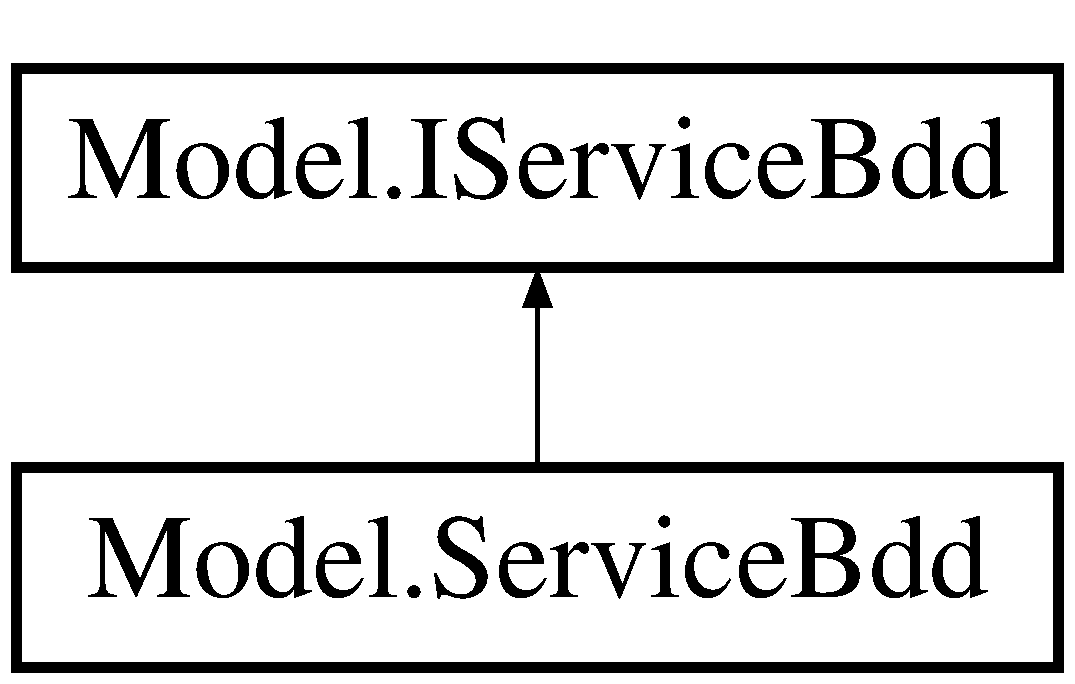
\includegraphics[height=2.000000cm]{class_model_1_1_i_service_bdd}
\end{center}
\end{figure}


The documentation for this class was generated from the following file\-:\begin{DoxyCompactItemize}
\item 
C\-:/\-Users/dju/\-Documents/\-Visual Studio 2012/\-Projects/\-P\-P\-E/\-P\-P\-E3/\-Model/\hyperlink{_service_bdd_8cs}{Service\-Bdd.\-cs}\end{DoxyCompactItemize}

\hypertarget{interface_wpf_application_1_1_model_1_1_i_service_client}{\section{Wpf\-Application.\-Model.\-I\-Service\-Client Interface Reference}
\label{interface_wpf_application_1_1_model_1_1_i_service_client}\index{Wpf\-Application.\-Model.\-I\-Service\-Client@{Wpf\-Application.\-Model.\-I\-Service\-Client}}
}
Inheritance diagram for Wpf\-Application.\-Model.\-I\-Service\-Client\-:\begin{figure}[H]
\begin{center}
\leavevmode
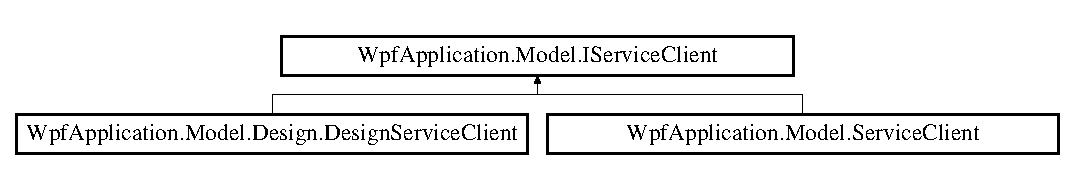
\includegraphics[height=1.830065cm]{interface_wpf_application_1_1_model_1_1_i_service_client}
\end{center}
\end{figure}
\subsection*{Public Member Functions}
\begin{DoxyCompactItemize}
\item 
\hyperlink{class_wpf_application_1_1_model_1_1_client}{Client} \hyperlink{interface_wpf_application_1_1_model_1_1_i_service_client_ab513b6cf91c0d31cfe37004ac5cf7e1e}{Charger} ()
\item 
List$<$ \hyperlink{class_wpf_application_1_1_model_1_1_client}{Client} $>$ \hyperlink{interface_wpf_application_1_1_model_1_1_i_service_client_a40ae24e7195bb27667e26ed27319c3e5}{Charger\-Tout} ()
\end{DoxyCompactItemize}


\subsection{Member Function Documentation}
\hypertarget{interface_wpf_application_1_1_model_1_1_i_service_client_ab513b6cf91c0d31cfe37004ac5cf7e1e}{\index{Wpf\-Application\-::\-Model\-::\-I\-Service\-Client@{Wpf\-Application\-::\-Model\-::\-I\-Service\-Client}!Charger@{Charger}}
\index{Charger@{Charger}!WpfApplication::Model::IServiceClient@{Wpf\-Application\-::\-Model\-::\-I\-Service\-Client}}
\subsubsection[{Charger}]{\setlength{\rightskip}{0pt plus 5cm}{\bf Client} Wpf\-Application.\-Model.\-I\-Service\-Client.\-Charger (
\begin{DoxyParamCaption}
{}
\end{DoxyParamCaption}
)}}\label{interface_wpf_application_1_1_model_1_1_i_service_client_ab513b6cf91c0d31cfe37004ac5cf7e1e}


Implemented in \hyperlink{class_wpf_application_1_1_model_1_1_design_1_1_design_service_client_a53e0167efe1963da87880b2aad52f8d1}{Wpf\-Application.\-Model.\-Design.\-Design\-Service\-Client}, and \hyperlink{class_wpf_application_1_1_model_1_1_service_client_aa018b0dfc38292ba0e1bf41715914d12}{Wpf\-Application.\-Model.\-Service\-Client}.

\hypertarget{interface_wpf_application_1_1_model_1_1_i_service_client_a40ae24e7195bb27667e26ed27319c3e5}{\index{Wpf\-Application\-::\-Model\-::\-I\-Service\-Client@{Wpf\-Application\-::\-Model\-::\-I\-Service\-Client}!Charger\-Tout@{Charger\-Tout}}
\index{Charger\-Tout@{Charger\-Tout}!WpfApplication::Model::IServiceClient@{Wpf\-Application\-::\-Model\-::\-I\-Service\-Client}}
\subsubsection[{Charger\-Tout}]{\setlength{\rightskip}{0pt plus 5cm}List$<${\bf Client}$>$ Wpf\-Application.\-Model.\-I\-Service\-Client.\-Charger\-Tout (
\begin{DoxyParamCaption}
{}
\end{DoxyParamCaption}
)}}\label{interface_wpf_application_1_1_model_1_1_i_service_client_a40ae24e7195bb27667e26ed27319c3e5}


Implemented in \hyperlink{class_wpf_application_1_1_model_1_1_design_1_1_design_service_client_adfe9e15a5cb29e6f1de7c6e30f494004}{Wpf\-Application.\-Model.\-Design.\-Design\-Service\-Client}, and \hyperlink{class_wpf_application_1_1_model_1_1_service_client_ac0b022539676651b790b38762026f0f1}{Wpf\-Application.\-Model.\-Service\-Client}.



The documentation for this interface was generated from the following file\-:\begin{DoxyCompactItemize}
\item 
C\-:/\-Users/dju/\-Documents/\-Visual Studio 2012/\-Projects/\-P\-P\-E/\-P\-P\-E3/\-Wpf\-Application/\-Model/\hyperlink{_i_service_client_8cs}{I\-Service\-Client.\-cs}\end{DoxyCompactItemize}

\hypertarget{class_wpf_application_1_1_view_1_1_list_window}{\section{Wpf\-Application.\-View.\-List\-Window Class Reference}
\label{class_wpf_application_1_1_view_1_1_list_window}\index{Wpf\-Application.\-View.\-List\-Window@{Wpf\-Application.\-View.\-List\-Window}}
}


\hyperlink{class_wpf_application_1_1_view_1_1_list_window}{List\-Window}  


Inheritance diagram for Wpf\-Application.\-View.\-List\-Window\-:\begin{figure}[H]
\begin{center}
\leavevmode
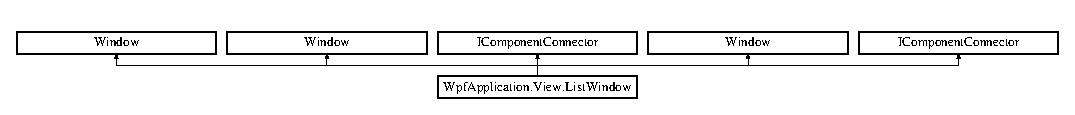
\includegraphics[height=1.098039cm]{class_wpf_application_1_1_view_1_1_list_window}
\end{center}
\end{figure}
\subsection*{Public Member Functions}
\begin{DoxyCompactItemize}
\item 
void \hyperlink{class_wpf_application_1_1_view_1_1_list_window_a696733c72718c7b5d8c6cb3adedc2f5c}{Initialize\-Component} ()
\begin{DoxyCompactList}\small\item\em Initialize\-Component \end{DoxyCompactList}\item 
void \hyperlink{class_wpf_application_1_1_view_1_1_list_window_a696733c72718c7b5d8c6cb3adedc2f5c}{Initialize\-Component} ()
\begin{DoxyCompactList}\small\item\em Initialize\-Component \end{DoxyCompactList}\item 
\hyperlink{class_wpf_application_1_1_view_1_1_list_window_af0e41aee8a50c9b68264bd0ac74ecd21}{List\-Window} ()
\end{DoxyCompactItemize}


\subsection{Detailed Description}
\hyperlink{class_wpf_application_1_1_view_1_1_list_window}{List\-Window} 

Logique d'interaction pour List\-Window.\-xaml 

\subsection{Constructor \& Destructor Documentation}
\hypertarget{class_wpf_application_1_1_view_1_1_list_window_af0e41aee8a50c9b68264bd0ac74ecd21}{\index{Wpf\-Application\-::\-View\-::\-List\-Window@{Wpf\-Application\-::\-View\-::\-List\-Window}!List\-Window@{List\-Window}}
\index{List\-Window@{List\-Window}!WpfApplication::View::ListWindow@{Wpf\-Application\-::\-View\-::\-List\-Window}}
\subsubsection[{List\-Window}]{\setlength{\rightskip}{0pt plus 5cm}Wpf\-Application.\-View.\-List\-Window.\-List\-Window (
\begin{DoxyParamCaption}
{}
\end{DoxyParamCaption}
)}}\label{class_wpf_application_1_1_view_1_1_list_window_af0e41aee8a50c9b68264bd0ac74ecd21}


\subsection{Member Function Documentation}
\hypertarget{class_wpf_application_1_1_view_1_1_list_window_a696733c72718c7b5d8c6cb3adedc2f5c}{\index{Wpf\-Application\-::\-View\-::\-List\-Window@{Wpf\-Application\-::\-View\-::\-List\-Window}!Initialize\-Component@{Initialize\-Component}}
\index{Initialize\-Component@{Initialize\-Component}!WpfApplication::View::ListWindow@{Wpf\-Application\-::\-View\-::\-List\-Window}}
\subsubsection[{Initialize\-Component}]{\setlength{\rightskip}{0pt plus 5cm}void Wpf\-Application.\-View.\-List\-Window.\-Initialize\-Component (
\begin{DoxyParamCaption}
{}
\end{DoxyParamCaption}
)}}\label{class_wpf_application_1_1_view_1_1_list_window_a696733c72718c7b5d8c6cb3adedc2f5c}


Initialize\-Component 

\hypertarget{class_wpf_application_1_1_view_1_1_list_window_a696733c72718c7b5d8c6cb3adedc2f5c}{\index{Wpf\-Application\-::\-View\-::\-List\-Window@{Wpf\-Application\-::\-View\-::\-List\-Window}!Initialize\-Component@{Initialize\-Component}}
\index{Initialize\-Component@{Initialize\-Component}!WpfApplication::View::ListWindow@{Wpf\-Application\-::\-View\-::\-List\-Window}}
\subsubsection[{Initialize\-Component}]{\setlength{\rightskip}{0pt plus 5cm}void Wpf\-Application.\-View.\-List\-Window.\-Initialize\-Component (
\begin{DoxyParamCaption}
{}
\end{DoxyParamCaption}
)}}\label{class_wpf_application_1_1_view_1_1_list_window_a696733c72718c7b5d8c6cb3adedc2f5c}


Initialize\-Component 



The documentation for this class was generated from the following files\-:\begin{DoxyCompactItemize}
\item 
C\-:/\-Users/dju/\-Documents/\-Visual Studio 2012/\-Projects/\-P\-P\-E/\-P\-P\-E3/\-Wpf\-Application/obj/\-Debug/\-View/\hyperlink{_list_window_8g_8cs}{List\-Window.\-g.\-cs}\item 
C\-:/\-Users/dju/\-Documents/\-Visual Studio 2012/\-Projects/\-P\-P\-E/\-P\-P\-E3/\-Wpf\-Application/obj/\-Debug/\-View/\hyperlink{_list_window_8g_8i_8cs}{List\-Window.\-g.\-i.\-cs}\item 
C\-:/\-Users/dju/\-Documents/\-Visual Studio 2012/\-Projects/\-P\-P\-E/\-P\-P\-E3/\-Wpf\-Application/\-View/\hyperlink{_list_window_8xaml_8cs}{List\-Window.\-xaml.\-cs}\end{DoxyCompactItemize}

\hypertarget{class_wpf_application_1_1_view_model_1_1_list_window_view_model}{\section{Wpf\-Application.\-View\-Model.\-List\-Window\-View\-Model Class Reference}
\label{class_wpf_application_1_1_view_model_1_1_list_window_view_model}\index{Wpf\-Application.\-View\-Model.\-List\-Window\-View\-Model@{Wpf\-Application.\-View\-Model.\-List\-Window\-View\-Model}}
}
Inheritance diagram for Wpf\-Application.\-View\-Model.\-List\-Window\-View\-Model\-:\begin{figure}[H]
\begin{center}
\leavevmode
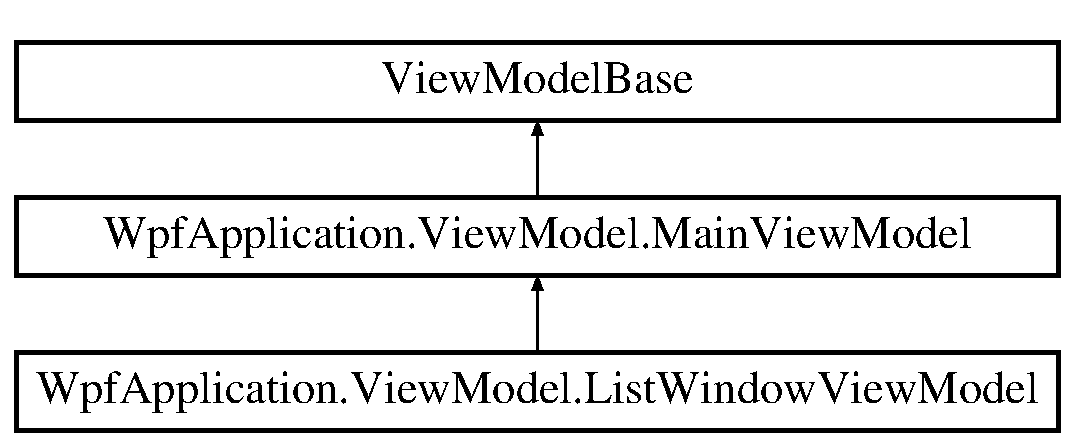
\includegraphics[height=3.000000cm]{class_wpf_application_1_1_view_model_1_1_list_window_view_model}
\end{center}
\end{figure}
\subsection*{Public Member Functions}
\begin{DoxyCompactItemize}
\item 
\hyperlink{class_wpf_application_1_1_view_model_1_1_list_window_view_model_a9eebaa1b58b8eee31763254332b733e1}{List\-Window\-View\-Model} (\hyperlink{interface_wpf_application_1_1_model_1_1_i_service_client}{I\-Service\-Client} service)
\end{DoxyCompactItemize}
\subsection*{Properties}
\begin{DoxyCompactItemize}
\item 
List$<$ \hyperlink{class_wpf_application_1_1_model_1_1_client}{Client} $>$ \hyperlink{class_wpf_application_1_1_view_model_1_1_list_window_view_model_a971a86a9000bf6c012967e817f59a2c4}{Liste\-Clients}\hspace{0.3cm}{\ttfamily  \mbox{[}get, set\mbox{]}}
\item 
I\-Command \hyperlink{class_wpf_application_1_1_view_model_1_1_list_window_view_model_a08034eb12e314399e69dbf09850fc1fc}{Qui\-Suis\-Je\-Command}\hspace{0.3cm}{\ttfamily  \mbox{[}get, set\mbox{]}}
\end{DoxyCompactItemize}


\subsection{Constructor \& Destructor Documentation}
\hypertarget{class_wpf_application_1_1_view_model_1_1_list_window_view_model_a9eebaa1b58b8eee31763254332b733e1}{\index{Wpf\-Application\-::\-View\-Model\-::\-List\-Window\-View\-Model@{Wpf\-Application\-::\-View\-Model\-::\-List\-Window\-View\-Model}!List\-Window\-View\-Model@{List\-Window\-View\-Model}}
\index{List\-Window\-View\-Model@{List\-Window\-View\-Model}!WpfApplication::ViewModel::ListWindowViewModel@{Wpf\-Application\-::\-View\-Model\-::\-List\-Window\-View\-Model}}
\subsubsection[{List\-Window\-View\-Model}]{\setlength{\rightskip}{0pt plus 5cm}Wpf\-Application.\-View\-Model.\-List\-Window\-View\-Model.\-List\-Window\-View\-Model (
\begin{DoxyParamCaption}
\item[{{\bf I\-Service\-Client}}]{service}
\end{DoxyParamCaption}
)}}\label{class_wpf_application_1_1_view_model_1_1_list_window_view_model_a9eebaa1b58b8eee31763254332b733e1}


\subsection{Property Documentation}
\hypertarget{class_wpf_application_1_1_view_model_1_1_list_window_view_model_a971a86a9000bf6c012967e817f59a2c4}{\index{Wpf\-Application\-::\-View\-Model\-::\-List\-Window\-View\-Model@{Wpf\-Application\-::\-View\-Model\-::\-List\-Window\-View\-Model}!Liste\-Clients@{Liste\-Clients}}
\index{Liste\-Clients@{Liste\-Clients}!WpfApplication::ViewModel::ListWindowViewModel@{Wpf\-Application\-::\-View\-Model\-::\-List\-Window\-View\-Model}}
\subsubsection[{Liste\-Clients}]{\setlength{\rightskip}{0pt plus 5cm}List$<${\bf Client}$>$ Wpf\-Application.\-View\-Model.\-List\-Window\-View\-Model.\-Liste\-Clients\hspace{0.3cm}{\ttfamily [get]}, {\ttfamily [set]}}}\label{class_wpf_application_1_1_view_model_1_1_list_window_view_model_a971a86a9000bf6c012967e817f59a2c4}
\hypertarget{class_wpf_application_1_1_view_model_1_1_list_window_view_model_a08034eb12e314399e69dbf09850fc1fc}{\index{Wpf\-Application\-::\-View\-Model\-::\-List\-Window\-View\-Model@{Wpf\-Application\-::\-View\-Model\-::\-List\-Window\-View\-Model}!Qui\-Suis\-Je\-Command@{Qui\-Suis\-Je\-Command}}
\index{Qui\-Suis\-Je\-Command@{Qui\-Suis\-Je\-Command}!WpfApplication::ViewModel::ListWindowViewModel@{Wpf\-Application\-::\-View\-Model\-::\-List\-Window\-View\-Model}}
\subsubsection[{Qui\-Suis\-Je\-Command}]{\setlength{\rightskip}{0pt plus 5cm}I\-Command Wpf\-Application.\-View\-Model.\-List\-Window\-View\-Model.\-Qui\-Suis\-Je\-Command\hspace{0.3cm}{\ttfamily [get]}, {\ttfamily [set]}}}\label{class_wpf_application_1_1_view_model_1_1_list_window_view_model_a08034eb12e314399e69dbf09850fc1fc}


The documentation for this class was generated from the following file\-:\begin{DoxyCompactItemize}
\item 
C\-:/\-Users/dju/\-Documents/\-Visual Studio 2012/\-Projects/\-P\-P\-E/\-P\-P\-E3/\-Wpf\-Application/\-View\-Model/\hyperlink{_list_window_view_model_8cs}{List\-Window\-View\-Model.\-cs}\end{DoxyCompactItemize}

\hypertarget{class_wpf_application_1_1_login_control}{\section{Wpf\-Application.\-Login\-Control Class Reference}
\label{class_wpf_application_1_1_login_control}\index{Wpf\-Application.\-Login\-Control@{Wpf\-Application.\-Login\-Control}}
}


\hyperlink{class_wpf_application_1_1_login_control}{Login\-Control}  


Inheritance diagram for Wpf\-Application.\-Login\-Control\-:\begin{figure}[H]
\begin{center}
\leavevmode
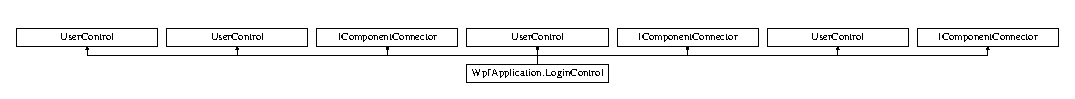
\includegraphics[height=0.883978cm]{class_wpf_application_1_1_login_control}
\end{center}
\end{figure}
\subsection*{Public Member Functions}
\begin{DoxyCompactItemize}
\item 
void \hyperlink{class_wpf_application_1_1_login_control_a62d93567bf185939bfc48026ab715d24}{Initialize\-Component} ()
\begin{DoxyCompactList}\small\item\em Initialize\-Component \end{DoxyCompactList}\item 
void \hyperlink{class_wpf_application_1_1_login_control_a62d93567bf185939bfc48026ab715d24}{Initialize\-Component} ()
\begin{DoxyCompactList}\small\item\em Initialize\-Component \end{DoxyCompactList}\item 
void \hyperlink{class_wpf_application_1_1_login_control_a62d93567bf185939bfc48026ab715d24}{Initialize\-Component} ()
\begin{DoxyCompactList}\small\item\em Initialize\-Component \end{DoxyCompactList}\item 
\hyperlink{class_wpf_application_1_1_login_control_abeed066cd62a32a76bdbe5e520d52da4}{Login\-Control} ()
\end{DoxyCompactItemize}


\subsection{Detailed Description}
\hyperlink{class_wpf_application_1_1_login_control}{Login\-Control} 

Logique d'interaction pour Login\-Control.\-xaml 

\subsection{Constructor \& Destructor Documentation}
\hypertarget{class_wpf_application_1_1_login_control_abeed066cd62a32a76bdbe5e520d52da4}{\index{Wpf\-Application\-::\-Login\-Control@{Wpf\-Application\-::\-Login\-Control}!Login\-Control@{Login\-Control}}
\index{Login\-Control@{Login\-Control}!WpfApplication::LoginControl@{Wpf\-Application\-::\-Login\-Control}}
\subsubsection[{Login\-Control}]{\setlength{\rightskip}{0pt plus 5cm}Wpf\-Application.\-Login\-Control.\-Login\-Control (
\begin{DoxyParamCaption}
{}
\end{DoxyParamCaption}
)}}\label{class_wpf_application_1_1_login_control_abeed066cd62a32a76bdbe5e520d52da4}


\subsection{Member Function Documentation}
\hypertarget{class_wpf_application_1_1_login_control_a62d93567bf185939bfc48026ab715d24}{\index{Wpf\-Application\-::\-Login\-Control@{Wpf\-Application\-::\-Login\-Control}!Initialize\-Component@{Initialize\-Component}}
\index{Initialize\-Component@{Initialize\-Component}!WpfApplication::LoginControl@{Wpf\-Application\-::\-Login\-Control}}
\subsubsection[{Initialize\-Component}]{\setlength{\rightskip}{0pt plus 5cm}void Wpf\-Application.\-Login\-Control.\-Initialize\-Component (
\begin{DoxyParamCaption}
{}
\end{DoxyParamCaption}
)}}\label{class_wpf_application_1_1_login_control_a62d93567bf185939bfc48026ab715d24}


Initialize\-Component 

\hypertarget{class_wpf_application_1_1_login_control_a62d93567bf185939bfc48026ab715d24}{\index{Wpf\-Application\-::\-Login\-Control@{Wpf\-Application\-::\-Login\-Control}!Initialize\-Component@{Initialize\-Component}}
\index{Initialize\-Component@{Initialize\-Component}!WpfApplication::LoginControl@{Wpf\-Application\-::\-Login\-Control}}
\subsubsection[{Initialize\-Component}]{\setlength{\rightskip}{0pt plus 5cm}void Wpf\-Application.\-Login\-Control.\-Initialize\-Component (
\begin{DoxyParamCaption}
{}
\end{DoxyParamCaption}
)}}\label{class_wpf_application_1_1_login_control_a62d93567bf185939bfc48026ab715d24}


Initialize\-Component 

\hypertarget{class_wpf_application_1_1_login_control_a62d93567bf185939bfc48026ab715d24}{\index{Wpf\-Application\-::\-Login\-Control@{Wpf\-Application\-::\-Login\-Control}!Initialize\-Component@{Initialize\-Component}}
\index{Initialize\-Component@{Initialize\-Component}!WpfApplication::LoginControl@{Wpf\-Application\-::\-Login\-Control}}
\subsubsection[{Initialize\-Component}]{\setlength{\rightskip}{0pt plus 5cm}void Wpf\-Application.\-Login\-Control.\-Initialize\-Component (
\begin{DoxyParamCaption}
{}
\end{DoxyParamCaption}
)}}\label{class_wpf_application_1_1_login_control_a62d93567bf185939bfc48026ab715d24}


Initialize\-Component 



The documentation for this class was generated from the following files\-:\begin{DoxyCompactItemize}
\item 
C\-:/\-Users/dju/\-Documents/\-Visual Studio 2012/\-Projects/\-P\-P\-E/\-P\-P\-E3/\-Wpf\-Application/obj/\-Debug/\hyperlink{_login_control_8g_8i_8cs}{Login\-Control.\-g.\-i.\-cs}\item 
C\-:/\-Users/dju/\-Documents/\-Visual Studio 2012/\-Projects/\-P\-P\-E/\-P\-P\-E3/\-Wpf\-Application/obj/\-Debug/\-View/\hyperlink{_login_control_8g_8cs}{Login\-Control.\-g.\-cs}\item 
C\-:/\-Users/dju/\-Documents/\-Visual Studio 2012/\-Projects/\-P\-P\-E/\-P\-P\-E3/\-Wpf\-Application/\-View/\hyperlink{_login_control_8xaml_8cs}{Login\-Control.\-xaml.\-cs}\end{DoxyCompactItemize}

\hypertarget{struct_wpf_application_1_1_view_model_1_1_login_infos_struct}{\section{Wpf\-Application.\-View\-Model.\-Login\-Infos\-Struct Struct Reference}
\label{struct_wpf_application_1_1_view_model_1_1_login_infos_struct}\index{Wpf\-Application.\-View\-Model.\-Login\-Infos\-Struct@{Wpf\-Application.\-View\-Model.\-Login\-Infos\-Struct}}
}
\subsection*{Properties}
\begin{DoxyCompactItemize}
\item 
string \hyperlink{struct_wpf_application_1_1_view_model_1_1_login_infos_struct_a2891a1643015a3c1c8d67690699c4fea}{Username}\hspace{0.3cm}{\ttfamily  \mbox{[}get, set\mbox{]}}
\item 
string \hyperlink{struct_wpf_application_1_1_view_model_1_1_login_infos_struct_afa77847ff79f91b1bb2e8ae20b3431cb}{Mdp}\hspace{0.3cm}{\ttfamily  \mbox{[}get, set\mbox{]}}
\end{DoxyCompactItemize}


\subsection{Property Documentation}
\hypertarget{struct_wpf_application_1_1_view_model_1_1_login_infos_struct_afa77847ff79f91b1bb2e8ae20b3431cb}{\index{Wpf\-Application\-::\-View\-Model\-::\-Login\-Infos\-Struct@{Wpf\-Application\-::\-View\-Model\-::\-Login\-Infos\-Struct}!Mdp@{Mdp}}
\index{Mdp@{Mdp}!WpfApplication::ViewModel::LoginInfosStruct@{Wpf\-Application\-::\-View\-Model\-::\-Login\-Infos\-Struct}}
\subsubsection[{Mdp}]{\setlength{\rightskip}{0pt plus 5cm}string Wpf\-Application.\-View\-Model.\-Login\-Infos\-Struct.\-Mdp\hspace{0.3cm}{\ttfamily [get]}, {\ttfamily [set]}}}\label{struct_wpf_application_1_1_view_model_1_1_login_infos_struct_afa77847ff79f91b1bb2e8ae20b3431cb}
\hypertarget{struct_wpf_application_1_1_view_model_1_1_login_infos_struct_a2891a1643015a3c1c8d67690699c4fea}{\index{Wpf\-Application\-::\-View\-Model\-::\-Login\-Infos\-Struct@{Wpf\-Application\-::\-View\-Model\-::\-Login\-Infos\-Struct}!Username@{Username}}
\index{Username@{Username}!WpfApplication::ViewModel::LoginInfosStruct@{Wpf\-Application\-::\-View\-Model\-::\-Login\-Infos\-Struct}}
\subsubsection[{Username}]{\setlength{\rightskip}{0pt plus 5cm}string Wpf\-Application.\-View\-Model.\-Login\-Infos\-Struct.\-Username\hspace{0.3cm}{\ttfamily [get]}, {\ttfamily [set]}}}\label{struct_wpf_application_1_1_view_model_1_1_login_infos_struct_a2891a1643015a3c1c8d67690699c4fea}


The documentation for this struct was generated from the following file\-:\begin{DoxyCompactItemize}
\item 
C\-:/\-Users/dju/\-Documents/\-Visual Studio 2012/\-Projects/\-P\-P\-E/\-P\-P\-E3/\-Wpf\-Application/\-View\-Model/\hyperlink{_login_view_model_8cs}{Login\-View\-Model.\-cs}\end{DoxyCompactItemize}

\hypertarget{class_wpf_application_1_1_view_1_1_login_view}{\section{Wpf\-Application.\-View.\-Login\-View Class Reference}
\label{class_wpf_application_1_1_view_1_1_login_view}\index{Wpf\-Application.\-View.\-Login\-View@{Wpf\-Application.\-View.\-Login\-View}}
}


\hyperlink{class_wpf_application_1_1_view_1_1_login_view}{Login\-View}  


Inheritance diagram for Wpf\-Application.\-View.\-Login\-View\-:\begin{figure}[H]
\begin{center}
\leavevmode
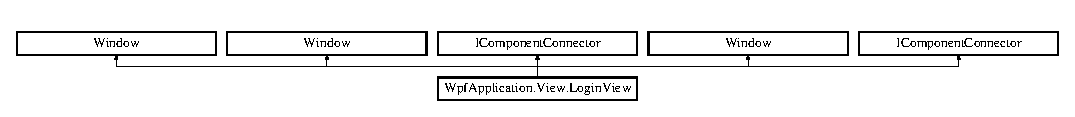
\includegraphics[height=1.120000cm]{class_wpf_application_1_1_view_1_1_login_view}
\end{center}
\end{figure}
\subsection*{Public Member Functions}
\begin{DoxyCompactItemize}
\item 
void \hyperlink{class_wpf_application_1_1_view_1_1_login_view_a93058e3538e875f4ebf62821e8b68eb6}{Initialize\-Component} ()
\begin{DoxyCompactList}\small\item\em Initialize\-Component \end{DoxyCompactList}\item 
void \hyperlink{class_wpf_application_1_1_view_1_1_login_view_a93058e3538e875f4ebf62821e8b68eb6}{Initialize\-Component} ()
\begin{DoxyCompactList}\small\item\em Initialize\-Component \end{DoxyCompactList}\item 
\hyperlink{class_wpf_application_1_1_view_1_1_login_view_a080dda3e07f2d5814f7fc6fc484cb1e1}{Login\-View} ()
\end{DoxyCompactItemize}


\subsection{Detailed Description}
\hyperlink{class_wpf_application_1_1_view_1_1_login_view}{Login\-View} 

Logique d'interaction pour Login\-View.\-xaml 

\subsection{Constructor \& Destructor Documentation}
\hypertarget{class_wpf_application_1_1_view_1_1_login_view_a080dda3e07f2d5814f7fc6fc484cb1e1}{\index{Wpf\-Application\-::\-View\-::\-Login\-View@{Wpf\-Application\-::\-View\-::\-Login\-View}!Login\-View@{Login\-View}}
\index{Login\-View@{Login\-View}!WpfApplication::View::LoginView@{Wpf\-Application\-::\-View\-::\-Login\-View}}
\subsubsection[{Login\-View}]{\setlength{\rightskip}{0pt plus 5cm}Wpf\-Application.\-View.\-Login\-View.\-Login\-View (
\begin{DoxyParamCaption}
{}
\end{DoxyParamCaption}
)}}\label{class_wpf_application_1_1_view_1_1_login_view_a080dda3e07f2d5814f7fc6fc484cb1e1}


\subsection{Member Function Documentation}
\hypertarget{class_wpf_application_1_1_view_1_1_login_view_a93058e3538e875f4ebf62821e8b68eb6}{\index{Wpf\-Application\-::\-View\-::\-Login\-View@{Wpf\-Application\-::\-View\-::\-Login\-View}!Initialize\-Component@{Initialize\-Component}}
\index{Initialize\-Component@{Initialize\-Component}!WpfApplication::View::LoginView@{Wpf\-Application\-::\-View\-::\-Login\-View}}
\subsubsection[{Initialize\-Component}]{\setlength{\rightskip}{0pt plus 5cm}void Wpf\-Application.\-View.\-Login\-View.\-Initialize\-Component (
\begin{DoxyParamCaption}
{}
\end{DoxyParamCaption}
)}}\label{class_wpf_application_1_1_view_1_1_login_view_a93058e3538e875f4ebf62821e8b68eb6}


Initialize\-Component 

\hypertarget{class_wpf_application_1_1_view_1_1_login_view_a93058e3538e875f4ebf62821e8b68eb6}{\index{Wpf\-Application\-::\-View\-::\-Login\-View@{Wpf\-Application\-::\-View\-::\-Login\-View}!Initialize\-Component@{Initialize\-Component}}
\index{Initialize\-Component@{Initialize\-Component}!WpfApplication::View::LoginView@{Wpf\-Application\-::\-View\-::\-Login\-View}}
\subsubsection[{Initialize\-Component}]{\setlength{\rightskip}{0pt plus 5cm}void Wpf\-Application.\-View.\-Login\-View.\-Initialize\-Component (
\begin{DoxyParamCaption}
{}
\end{DoxyParamCaption}
)}}\label{class_wpf_application_1_1_view_1_1_login_view_a93058e3538e875f4ebf62821e8b68eb6}


Initialize\-Component 



The documentation for this class was generated from the following files\-:\begin{DoxyCompactItemize}
\item 
C\-:/\-Users/dju/\-Documents/\-Visual Studio 2012/\-Projects/\-P\-P\-E/\-P\-P\-E3/\-Wpf\-Application/obj/\-Debug/\-View/\hyperlink{_login_view_8g_8cs}{Login\-View.\-g.\-cs}\item 
C\-:/\-Users/dju/\-Documents/\-Visual Studio 2012/\-Projects/\-P\-P\-E/\-P\-P\-E3/\-Wpf\-Application/obj/\-Debug/\-View/\hyperlink{_login_view_8g_8i_8cs}{Login\-View.\-g.\-i.\-cs}\item 
C\-:/\-Users/dju/\-Documents/\-Visual Studio 2012/\-Projects/\-P\-P\-E/\-P\-P\-E3/\-Wpf\-Application/\-View/\hyperlink{_login_view_8xaml_8cs}{Login\-View.\-xaml.\-cs}\end{DoxyCompactItemize}

\hypertarget{class_wpf_application_1_1_view_model_1_1_login_view_model}{\section{Wpf\-Application.\-View\-Model.\-Login\-View\-Model Class Reference}
\label{class_wpf_application_1_1_view_model_1_1_login_view_model}\index{Wpf\-Application.\-View\-Model.\-Login\-View\-Model@{Wpf\-Application.\-View\-Model.\-Login\-View\-Model}}
}
Inheritance diagram for Wpf\-Application.\-View\-Model.\-Login\-View\-Model\-:\begin{figure}[H]
\begin{center}
\leavevmode
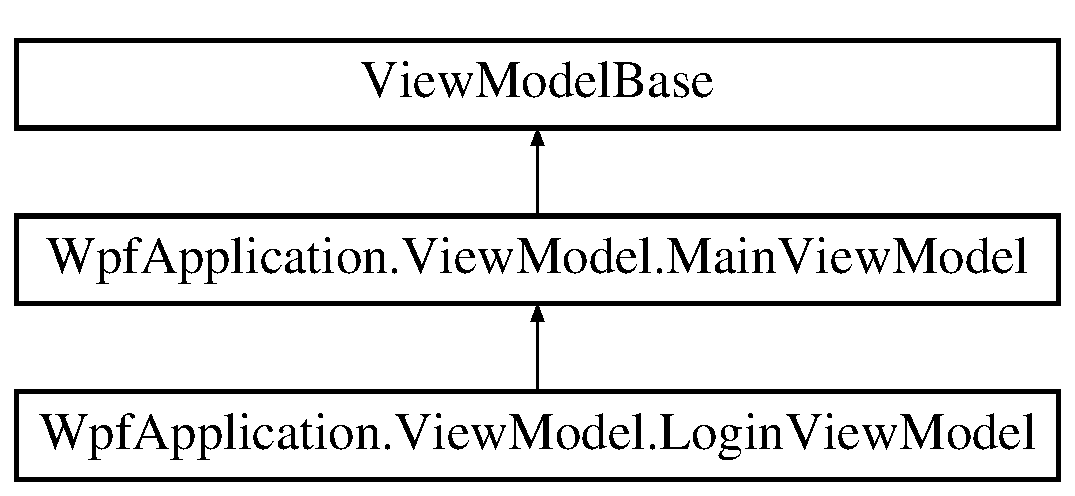
\includegraphics[height=3.000000cm]{class_wpf_application_1_1_view_model_1_1_login_view_model}
\end{center}
\end{figure}
\subsection*{Public Member Functions}
\begin{DoxyCompactItemize}
\item 
\hyperlink{class_wpf_application_1_1_view_model_1_1_login_view_model_afe8708360a4ee79d5ee9662a64d17140}{Login\-View\-Model} (\hyperlink{interface_wpf_application_1_1_model_1_1_i_service_client}{I\-Service\-Client} service)
\begin{DoxyCompactList}\small\item\em Constructeur \end{DoxyCompactList}\end{DoxyCompactItemize}
\subsection*{Properties}
\begin{DoxyCompactItemize}
\item 
I\-Command \hyperlink{class_wpf_application_1_1_view_model_1_1_login_view_model_ae38da2719079c1cd5e7b490b2f148da7}{Login\-Text\-Changed\-Command}\hspace{0.3cm}{\ttfamily  \mbox{[}get\mbox{]}}
\item 
I\-Command \hyperlink{class_wpf_application_1_1_view_model_1_1_login_view_model_ada946f5d652607c5bc0ee7304448521e}{Mdp\-Text\-Changed\-Command}\hspace{0.3cm}{\ttfamily  \mbox{[}get\mbox{]}}
\item 
I\-Command \hyperlink{class_wpf_application_1_1_view_model_1_1_login_view_model_abc7d5ebea644ef08fa0ce5c8507b3403}{Sign\-In\-Command}\hspace{0.3cm}{\ttfamily  \mbox{[}get\mbox{]}}
\end{DoxyCompactItemize}


\subsection{Constructor \& Destructor Documentation}
\hypertarget{class_wpf_application_1_1_view_model_1_1_login_view_model_afe8708360a4ee79d5ee9662a64d17140}{\index{Wpf\-Application\-::\-View\-Model\-::\-Login\-View\-Model@{Wpf\-Application\-::\-View\-Model\-::\-Login\-View\-Model}!Login\-View\-Model@{Login\-View\-Model}}
\index{Login\-View\-Model@{Login\-View\-Model}!WpfApplication::ViewModel::LoginViewModel@{Wpf\-Application\-::\-View\-Model\-::\-Login\-View\-Model}}
\subsubsection[{Login\-View\-Model}]{\setlength{\rightskip}{0pt plus 5cm}Wpf\-Application.\-View\-Model.\-Login\-View\-Model.\-Login\-View\-Model (
\begin{DoxyParamCaption}
\item[{{\bf I\-Service\-Client}}]{service}
\end{DoxyParamCaption}
)}}\label{class_wpf_application_1_1_view_model_1_1_login_view_model_afe8708360a4ee79d5ee9662a64d17140}


Constructeur 



\subsection{Property Documentation}
\hypertarget{class_wpf_application_1_1_view_model_1_1_login_view_model_ae38da2719079c1cd5e7b490b2f148da7}{\index{Wpf\-Application\-::\-View\-Model\-::\-Login\-View\-Model@{Wpf\-Application\-::\-View\-Model\-::\-Login\-View\-Model}!Login\-Text\-Changed\-Command@{Login\-Text\-Changed\-Command}}
\index{Login\-Text\-Changed\-Command@{Login\-Text\-Changed\-Command}!WpfApplication::ViewModel::LoginViewModel@{Wpf\-Application\-::\-View\-Model\-::\-Login\-View\-Model}}
\subsubsection[{Login\-Text\-Changed\-Command}]{\setlength{\rightskip}{0pt plus 5cm}I\-Command Wpf\-Application.\-View\-Model.\-Login\-View\-Model.\-Login\-Text\-Changed\-Command\hspace{0.3cm}{\ttfamily [get]}}}\label{class_wpf_application_1_1_view_model_1_1_login_view_model_ae38da2719079c1cd5e7b490b2f148da7}
\hypertarget{class_wpf_application_1_1_view_model_1_1_login_view_model_ada946f5d652607c5bc0ee7304448521e}{\index{Wpf\-Application\-::\-View\-Model\-::\-Login\-View\-Model@{Wpf\-Application\-::\-View\-Model\-::\-Login\-View\-Model}!Mdp\-Text\-Changed\-Command@{Mdp\-Text\-Changed\-Command}}
\index{Mdp\-Text\-Changed\-Command@{Mdp\-Text\-Changed\-Command}!WpfApplication::ViewModel::LoginViewModel@{Wpf\-Application\-::\-View\-Model\-::\-Login\-View\-Model}}
\subsubsection[{Mdp\-Text\-Changed\-Command}]{\setlength{\rightskip}{0pt plus 5cm}I\-Command Wpf\-Application.\-View\-Model.\-Login\-View\-Model.\-Mdp\-Text\-Changed\-Command\hspace{0.3cm}{\ttfamily [get]}}}\label{class_wpf_application_1_1_view_model_1_1_login_view_model_ada946f5d652607c5bc0ee7304448521e}
\hypertarget{class_wpf_application_1_1_view_model_1_1_login_view_model_abc7d5ebea644ef08fa0ce5c8507b3403}{\index{Wpf\-Application\-::\-View\-Model\-::\-Login\-View\-Model@{Wpf\-Application\-::\-View\-Model\-::\-Login\-View\-Model}!Sign\-In\-Command@{Sign\-In\-Command}}
\index{Sign\-In\-Command@{Sign\-In\-Command}!WpfApplication::ViewModel::LoginViewModel@{Wpf\-Application\-::\-View\-Model\-::\-Login\-View\-Model}}
\subsubsection[{Sign\-In\-Command}]{\setlength{\rightskip}{0pt plus 5cm}I\-Command Wpf\-Application.\-View\-Model.\-Login\-View\-Model.\-Sign\-In\-Command\hspace{0.3cm}{\ttfamily [get]}}}\label{class_wpf_application_1_1_view_model_1_1_login_view_model_abc7d5ebea644ef08fa0ce5c8507b3403}


The documentation for this class was generated from the following file\-:\begin{DoxyCompactItemize}
\item 
C\-:/\-Users/dju/\-Documents/\-Visual Studio 2012/\-Projects/\-P\-P\-E/\-P\-P\-E3/\-Wpf\-Application/\-View\-Model/\hyperlink{_login_view_model_8cs}{Login\-View\-Model.\-cs}\end{DoxyCompactItemize}

\hypertarget{class_wpf_application_1_1_view_model_1_1_main_view_model}{\section{Wpf\-Application.\-View\-Model.\-Main\-View\-Model Class Reference}
\label{class_wpf_application_1_1_view_model_1_1_main_view_model}\index{Wpf\-Application.\-View\-Model.\-Main\-View\-Model@{Wpf\-Application.\-View\-Model.\-Main\-View\-Model}}
}


This class contains properties that the main \hyperlink{namespace_wpf_application_1_1_view}{View} can data bind to.  


Inheritance diagram for Wpf\-Application.\-View\-Model.\-Main\-View\-Model\-:\begin{figure}[H]
\begin{center}
\leavevmode
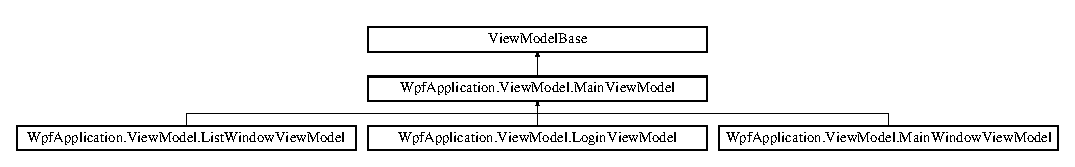
\includegraphics[height=1.800643cm]{class_wpf_application_1_1_view_model_1_1_main_view_model}
\end{center}
\end{figure}
\subsection*{Public Member Functions}
\begin{DoxyCompactItemize}
\item 
\hyperlink{class_wpf_application_1_1_view_model_1_1_main_view_model_a10d48f1102c37721d158217627222e4b}{Main\-View\-Model} ()
\begin{DoxyCompactList}\small\item\em Initializes a new instance of the \hyperlink{class_wpf_application_1_1_view_model_1_1_main_view_model}{Main\-View\-Model} class. \end{DoxyCompactList}\end{DoxyCompactItemize}


\subsection{Detailed Description}
This class contains properties that the main \hyperlink{namespace_wpf_application_1_1_view}{View} can data bind to. 

Use the {\bfseries mvvminpc} snippet to add bindable properties to this \hyperlink{namespace_wpf_application_1_1_view_model}{View\-Model}. 

You can also use Blend to data bind with the tool's support. 

See \href{http://www.galasoft.ch/mvvm}{\tt http\-://www.\-galasoft.\-ch/mvvm} 

\subsection{Constructor \& Destructor Documentation}
\hypertarget{class_wpf_application_1_1_view_model_1_1_main_view_model_a10d48f1102c37721d158217627222e4b}{\index{Wpf\-Application\-::\-View\-Model\-::\-Main\-View\-Model@{Wpf\-Application\-::\-View\-Model\-::\-Main\-View\-Model}!Main\-View\-Model@{Main\-View\-Model}}
\index{Main\-View\-Model@{Main\-View\-Model}!WpfApplication::ViewModel::MainViewModel@{Wpf\-Application\-::\-View\-Model\-::\-Main\-View\-Model}}
\subsubsection[{Main\-View\-Model}]{\setlength{\rightskip}{0pt plus 5cm}Wpf\-Application.\-View\-Model.\-Main\-View\-Model.\-Main\-View\-Model (
\begin{DoxyParamCaption}
{}
\end{DoxyParamCaption}
)}}\label{class_wpf_application_1_1_view_model_1_1_main_view_model_a10d48f1102c37721d158217627222e4b}


Initializes a new instance of the \hyperlink{class_wpf_application_1_1_view_model_1_1_main_view_model}{Main\-View\-Model} class. 



The documentation for this class was generated from the following file\-:\begin{DoxyCompactItemize}
\item 
C\-:/\-Users/dju/\-Documents/\-Visual Studio 2012/\-Projects/\-P\-P\-E/\-P\-P\-E3/\-Wpf\-Application/\-View\-Model/\hyperlink{_main_view_model_8cs}{Main\-View\-Model.\-cs}\end{DoxyCompactItemize}

\hypertarget{class_wpf_application_1_1_main_window}{\section{Wpf\-Application.\-Main\-Window Class Reference}
\label{class_wpf_application_1_1_main_window}\index{Wpf\-Application.\-Main\-Window@{Wpf\-Application.\-Main\-Window}}
}


\hyperlink{class_wpf_application_1_1_main_window}{Main\-Window}  


Inheritance diagram for Wpf\-Application.\-Main\-Window\-:\begin{figure}[H]
\begin{center}
\leavevmode
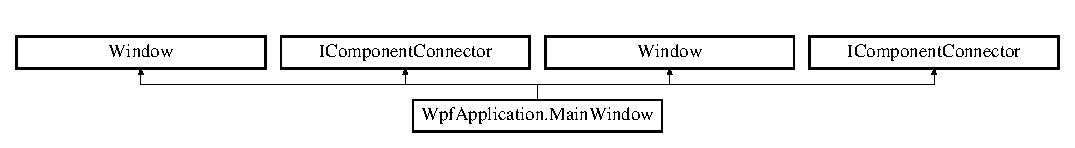
\includegraphics[height=1.546961cm]{class_wpf_application_1_1_main_window}
\end{center}
\end{figure}
\subsection*{Public Member Functions}
\begin{DoxyCompactItemize}
\item 
void \hyperlink{class_wpf_application_1_1_main_window_a45cac8c6a884abb12768797ccf07451f}{Initialize\-Component} ()
\begin{DoxyCompactList}\small\item\em Initialize\-Component \end{DoxyCompactList}\item 
void \hyperlink{class_wpf_application_1_1_main_window_a45cac8c6a884abb12768797ccf07451f}{Initialize\-Component} ()
\begin{DoxyCompactList}\small\item\em Initialize\-Component \end{DoxyCompactList}\end{DoxyCompactItemize}


\subsection{Detailed Description}
\hyperlink{class_wpf_application_1_1_main_window}{Main\-Window} 



\subsection{Member Function Documentation}
\hypertarget{class_wpf_application_1_1_main_window_a45cac8c6a884abb12768797ccf07451f}{\index{Wpf\-Application\-::\-Main\-Window@{Wpf\-Application\-::\-Main\-Window}!Initialize\-Component@{Initialize\-Component}}
\index{Initialize\-Component@{Initialize\-Component}!WpfApplication::MainWindow@{Wpf\-Application\-::\-Main\-Window}}
\subsubsection[{Initialize\-Component}]{\setlength{\rightskip}{0pt plus 5cm}void Wpf\-Application.\-Main\-Window.\-Initialize\-Component (
\begin{DoxyParamCaption}
{}
\end{DoxyParamCaption}
)}}\label{class_wpf_application_1_1_main_window_a45cac8c6a884abb12768797ccf07451f}


Initialize\-Component 

\hypertarget{class_wpf_application_1_1_main_window_a45cac8c6a884abb12768797ccf07451f}{\index{Wpf\-Application\-::\-Main\-Window@{Wpf\-Application\-::\-Main\-Window}!Initialize\-Component@{Initialize\-Component}}
\index{Initialize\-Component@{Initialize\-Component}!WpfApplication::MainWindow@{Wpf\-Application\-::\-Main\-Window}}
\subsubsection[{Initialize\-Component}]{\setlength{\rightskip}{0pt plus 5cm}void Wpf\-Application.\-Main\-Window.\-Initialize\-Component (
\begin{DoxyParamCaption}
{}
\end{DoxyParamCaption}
)}}\label{class_wpf_application_1_1_main_window_a45cac8c6a884abb12768797ccf07451f}


Initialize\-Component 



The documentation for this class was generated from the following file\-:\begin{DoxyCompactItemize}
\item 
C\-:/\-Users/dju/\-Documents/\-Visual Studio 2012/\-Projects/\-P\-P\-E/\-P\-P\-E3/\-Wpf\-Application/obj/\-Debug/\hyperlink{_main_window_8g_8i_8cs}{Main\-Window.\-g.\-i.\-cs}\end{DoxyCompactItemize}

\hypertarget{class_wpf_application_1_1_view_1_1_main_window}{\section{Wpf\-Application.\-View.\-Main\-Window Class Reference}
\label{class_wpf_application_1_1_view_1_1_main_window}\index{Wpf\-Application.\-View.\-Main\-Window@{Wpf\-Application.\-View.\-Main\-Window}}
}


\hyperlink{class_wpf_application_1_1_view_1_1_main_window}{Main\-Window}  


Inheritance diagram for Wpf\-Application.\-View.\-Main\-Window\-:\begin{figure}[H]
\begin{center}
\leavevmode
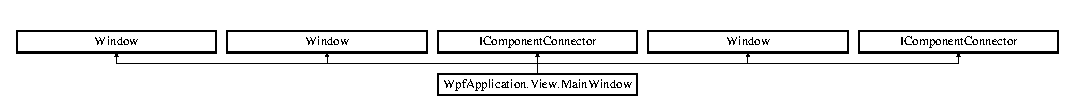
\includegraphics[height=1.051643cm]{class_wpf_application_1_1_view_1_1_main_window}
\end{center}
\end{figure}
\subsection*{Public Member Functions}
\begin{DoxyCompactItemize}
\item 
void \hyperlink{class_wpf_application_1_1_view_1_1_main_window_ada989bc9473ea0dfba99c402b94cf87d}{Initialize\-Component} ()
\begin{DoxyCompactList}\small\item\em Initialize\-Component \end{DoxyCompactList}\item 
void \hyperlink{class_wpf_application_1_1_view_1_1_main_window_ada989bc9473ea0dfba99c402b94cf87d}{Initialize\-Component} ()
\begin{DoxyCompactList}\small\item\em Initialize\-Component \end{DoxyCompactList}\item 
\hyperlink{class_wpf_application_1_1_view_1_1_main_window_ac2710c7546972b854e654ae059643e66}{Main\-Window} ()
\end{DoxyCompactItemize}


\subsection{Detailed Description}
\hyperlink{class_wpf_application_1_1_view_1_1_main_window}{Main\-Window} 

Logique d'interaction pour Main\-Window.\-xaml 

\subsection{Constructor \& Destructor Documentation}
\hypertarget{class_wpf_application_1_1_view_1_1_main_window_ac2710c7546972b854e654ae059643e66}{\index{Wpf\-Application\-::\-View\-::\-Main\-Window@{Wpf\-Application\-::\-View\-::\-Main\-Window}!Main\-Window@{Main\-Window}}
\index{Main\-Window@{Main\-Window}!WpfApplication::View::MainWindow@{Wpf\-Application\-::\-View\-::\-Main\-Window}}
\subsubsection[{Main\-Window}]{\setlength{\rightskip}{0pt plus 5cm}Wpf\-Application.\-View.\-Main\-Window.\-Main\-Window (
\begin{DoxyParamCaption}
{}
\end{DoxyParamCaption}
)}}\label{class_wpf_application_1_1_view_1_1_main_window_ac2710c7546972b854e654ae059643e66}


\subsection{Member Function Documentation}
\hypertarget{class_wpf_application_1_1_view_1_1_main_window_ada989bc9473ea0dfba99c402b94cf87d}{\index{Wpf\-Application\-::\-View\-::\-Main\-Window@{Wpf\-Application\-::\-View\-::\-Main\-Window}!Initialize\-Component@{Initialize\-Component}}
\index{Initialize\-Component@{Initialize\-Component}!WpfApplication::View::MainWindow@{Wpf\-Application\-::\-View\-::\-Main\-Window}}
\subsubsection[{Initialize\-Component}]{\setlength{\rightskip}{0pt plus 5cm}void Wpf\-Application.\-View.\-Main\-Window.\-Initialize\-Component (
\begin{DoxyParamCaption}
{}
\end{DoxyParamCaption}
)}}\label{class_wpf_application_1_1_view_1_1_main_window_ada989bc9473ea0dfba99c402b94cf87d}


Initialize\-Component 

\hypertarget{class_wpf_application_1_1_view_1_1_main_window_ada989bc9473ea0dfba99c402b94cf87d}{\index{Wpf\-Application\-::\-View\-::\-Main\-Window@{Wpf\-Application\-::\-View\-::\-Main\-Window}!Initialize\-Component@{Initialize\-Component}}
\index{Initialize\-Component@{Initialize\-Component}!WpfApplication::View::MainWindow@{Wpf\-Application\-::\-View\-::\-Main\-Window}}
\subsubsection[{Initialize\-Component}]{\setlength{\rightskip}{0pt plus 5cm}void Wpf\-Application.\-View.\-Main\-Window.\-Initialize\-Component (
\begin{DoxyParamCaption}
{}
\end{DoxyParamCaption}
)}}\label{class_wpf_application_1_1_view_1_1_main_window_ada989bc9473ea0dfba99c402b94cf87d}


Initialize\-Component 



The documentation for this class was generated from the following files\-:\begin{DoxyCompactItemize}
\item 
C\-:/\-Users/dju/\-Documents/\-Visual Studio 2012/\-Projects/\-P\-P\-E/\-P\-P\-E3/\-Wpf\-Application/obj/\-Debug/\-View/\hyperlink{_main_window_8g_8cs}{Main\-Window.\-g.\-cs}\item 
C\-:/\-Users/dju/\-Documents/\-Visual Studio 2012/\-Projects/\-P\-P\-E/\-P\-P\-E3/\-Wpf\-Application/obj/\-Debug/\-View/\hyperlink{_view_2_main_window_8g_8i_8cs}{Main\-Window.\-g.\-i.\-cs}\item 
C\-:/\-Users/dju/\-Documents/\-Visual Studio 2012/\-Projects/\-P\-P\-E/\-P\-P\-E3/\-Wpf\-Application/\-View/\hyperlink{_main_window_8xaml_8cs}{Main\-Window.\-xaml.\-cs}\end{DoxyCompactItemize}

\hypertarget{class_wpf_application_1_1_view_model_1_1_main_window_view_model}{\section{Wpf\-Application.\-View\-Model.\-Main\-Window\-View\-Model Class Reference}
\label{class_wpf_application_1_1_view_model_1_1_main_window_view_model}\index{Wpf\-Application.\-View\-Model.\-Main\-Window\-View\-Model@{Wpf\-Application.\-View\-Model.\-Main\-Window\-View\-Model}}
}
Inheritance diagram for Wpf\-Application.\-View\-Model.\-Main\-Window\-View\-Model\-:\begin{figure}[H]
\begin{center}
\leavevmode
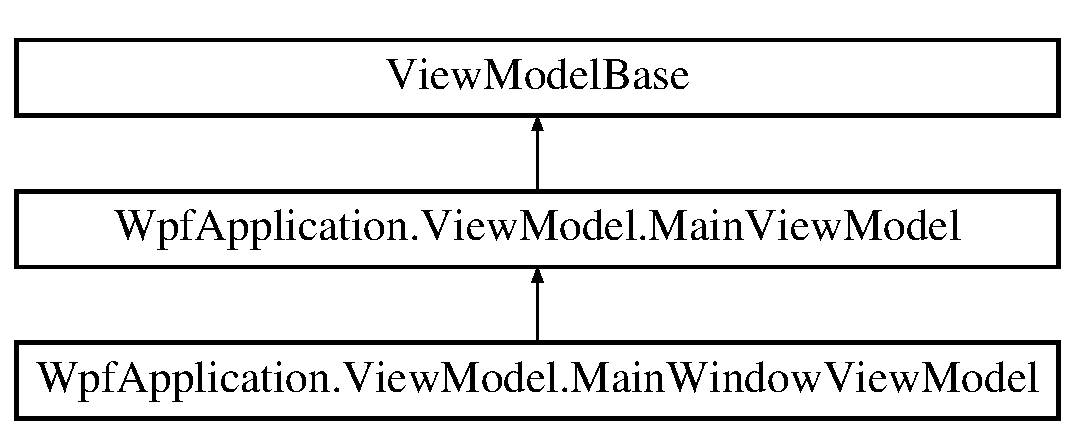
\includegraphics[height=3.000000cm]{class_wpf_application_1_1_view_model_1_1_main_window_view_model}
\end{center}
\end{figure}
\subsection*{Public Member Functions}
\begin{DoxyCompactItemize}
\item 
List$<$ \hyperlink{class_wpf_application_1_1_view_model_1_1_trans_1_1_col_trans}{Col\-Trans} $>$ \hyperlink{class_wpf_application_1_1_view_model_1_1_main_window_view_model_a6063564818bfdec1fbe87e6f0d3a91e1}{convert\-Col} (List$<$ \hyperlink{class_model_1_1_c_o_l_l_a_b_o_r_a_t_e_u_r}{C\-O\-L\-L\-A\-B\-O\-R\-A\-T\-E\-U\-R} $>$ list)
\item 
List$<$ \hyperlink{class_wpf_application_1_1_view_model_1_1_trans_1_1_rap_trans}{Rap\-Trans} $>$ \hyperlink{class_wpf_application_1_1_view_model_1_1_main_window_view_model_a8918e291a784522e1b3b39e2eb155696}{convert\-Rap} (List$<$ \hyperlink{class_model_1_1_r_a_p_p_o_r_t___d_e___v_i_s_i_t_e}{R\-A\-P\-P\-O\-R\-T\-\_\-\-D\-E\-\_\-\-V\-I\-S\-I\-T\-E} $>$ list)
\item 
List$<$ \hyperlink{class_wpf_application_1_1_view_model_1_1_trans_1_1_pra_trans}{Pra\-Trans} $>$ \hyperlink{class_wpf_application_1_1_view_model_1_1_main_window_view_model_aef1459769387db166cd60362723652e6}{convert\-Prat} (List$<$ \hyperlink{class_model_1_1_p_r_a_t_i_c_i_e_n}{P\-R\-A\-T\-I\-C\-I\-E\-N} $>$ list)
\item 
\hyperlink{class_wpf_application_1_1_view_model_1_1_main_window_view_model_a7ac6f627260aea5f5449c034bd73eb38}{Main\-Window\-View\-Model} (\hyperlink{interface_wpf_application_1_1_model_1_1_i_service_client}{I\-Service\-Client} service)
\begin{DoxyCompactList}\small\item\em Constructeur du View-\/\-Model \end{DoxyCompactList}\end{DoxyCompactItemize}
\subsection*{Properties}
\begin{DoxyCompactItemize}
\item 
\hyperlink{struct_wpf_application_1_1_view_model_1_1_filtre_struct}{Filtre\-Struct} \hyperlink{class_wpf_application_1_1_view_model_1_1_main_window_view_model_a01234e72909d01f98d245a48709d96bf}{Sfiltre}\hspace{0.3cm}{\ttfamily  \mbox{[}get, set\mbox{]}}
\item 
I\-Command \hyperlink{class_wpf_application_1_1_view_model_1_1_main_window_view_model_af9faf52029e4ef01aa4436d58548ca63}{Exit\-Command}\hspace{0.3cm}{\ttfamily  \mbox{[}get\mbox{]}}
\item 
I\-Command \hyperlink{class_wpf_application_1_1_view_model_1_1_main_window_view_model_a7c28181152e62d237a59d2f778c7ef0c}{Test\-Command}\hspace{0.3cm}{\ttfamily  \mbox{[}get\mbox{]}}
\item 
I\-Command \hyperlink{class_wpf_application_1_1_view_model_1_1_main_window_view_model_aea9aa9c929c10f71d89beb82d4fa26c1}{Excel\-Command}\hspace{0.3cm}{\ttfamily  \mbox{[}get\mbox{]}}
\item 
I\-Command \hyperlink{class_wpf_application_1_1_view_model_1_1_main_window_view_model_ab12838cb1154ad278bded6b4366f356f}{Filtre\-Command}\hspace{0.3cm}{\ttfamily  \mbox{[}get\mbox{]}}
\item 
I\-Command \hyperlink{class_wpf_application_1_1_view_model_1_1_main_window_view_model_a1b6ffad7c8cef7b0665ff73c8bdb01b7}{Selected\-Items\-Command}\hspace{0.3cm}{\ttfamily  \mbox{[}get\mbox{]}}
\item 
I\-Command \hyperlink{class_wpf_application_1_1_view_model_1_1_main_window_view_model_a3dda2a9013e1d4cba7864004866bd0d2}{Select\-Changed\-Command}\hspace{0.3cm}{\ttfamily  \mbox{[}get\mbox{]}}
\item 
I\-Command \hyperlink{class_wpf_application_1_1_view_model_1_1_main_window_view_model_a86bb2a58cef68a1dd3d1a9c8d403221b}{Text\-Changed\-Command}\hspace{0.3cm}{\ttfamily  \mbox{[}get\mbox{]}}
\item 
I\-Command \hyperlink{class_wpf_application_1_1_view_model_1_1_main_window_view_model_a437a4aeaf5952c6d8ad2bfc7c1219fdb}{Combo\-Sel\-Changed\-Command}\hspace{0.3cm}{\ttfamily  \mbox{[}get\mbox{]}}
\item 
List$<$ object $>$ \hyperlink{class_wpf_application_1_1_view_model_1_1_main_window_view_model_a7cbdf02ce36b41c52455837ea5f54b53}{Liste\-Sel}\hspace{0.3cm}{\ttfamily  \mbox{[}get, set\mbox{]}}
\item 
List$<$ string $>$ \hyperlink{class_wpf_application_1_1_view_model_1_1_main_window_view_model_a503e095c920ffa53134b69f9db7a0cd0}{Liste\-Filtres}\hspace{0.3cm}{\ttfamily  \mbox{[}get, set\mbox{]}}
\item 
List$<$ \hyperlink{class_wpf_application_1_1_view_model_1_1_trans_1_1_col_trans}{Col\-Trans} $>$ \hyperlink{class_wpf_application_1_1_view_model_1_1_main_window_view_model_a67f83abd9929d0022cb5de440f8f90ff}{Liste\-Col}\hspace{0.3cm}{\ttfamily  \mbox{[}get, set\mbox{]}}
\item 
List$<$ \hyperlink{class_wpf_application_1_1_view_model_1_1_trans_1_1_rap_trans}{Rap\-Trans} $>$ \hyperlink{class_wpf_application_1_1_view_model_1_1_main_window_view_model_abcc1152c3ac6999818a21102319636ac}{Liste\-Rap}\hspace{0.3cm}{\ttfamily  \mbox{[}get, set\mbox{]}}
\item 
List$<$ \hyperlink{class_wpf_application_1_1_view_model_1_1_trans_1_1_pra_trans}{Pra\-Trans} $>$ \hyperlink{class_wpf_application_1_1_view_model_1_1_main_window_view_model_a37280bec8e8e38711565a542a277bfe6}{Liste\-Prat}\hspace{0.3cm}{\ttfamily  \mbox{[}get, set\mbox{]}}
\end{DoxyCompactItemize}


\subsection{Constructor \& Destructor Documentation}
\hypertarget{class_wpf_application_1_1_view_model_1_1_main_window_view_model_a7ac6f627260aea5f5449c034bd73eb38}{\index{Wpf\-Application\-::\-View\-Model\-::\-Main\-Window\-View\-Model@{Wpf\-Application\-::\-View\-Model\-::\-Main\-Window\-View\-Model}!Main\-Window\-View\-Model@{Main\-Window\-View\-Model}}
\index{Main\-Window\-View\-Model@{Main\-Window\-View\-Model}!WpfApplication::ViewModel::MainWindowViewModel@{Wpf\-Application\-::\-View\-Model\-::\-Main\-Window\-View\-Model}}
\subsubsection[{Main\-Window\-View\-Model}]{\setlength{\rightskip}{0pt plus 5cm}Wpf\-Application.\-View\-Model.\-Main\-Window\-View\-Model.\-Main\-Window\-View\-Model (
\begin{DoxyParamCaption}
\item[{{\bf I\-Service\-Client}}]{service}
\end{DoxyParamCaption}
)}}\label{class_wpf_application_1_1_view_model_1_1_main_window_view_model_a7ac6f627260aea5f5449c034bd73eb38}


Constructeur du View-\/\-Model 


\begin{DoxyParams}{Parameters}
{\em service} & ???\\
\hline
\end{DoxyParams}


\subsection{Member Function Documentation}
\hypertarget{class_wpf_application_1_1_view_model_1_1_main_window_view_model_a6063564818bfdec1fbe87e6f0d3a91e1}{\index{Wpf\-Application\-::\-View\-Model\-::\-Main\-Window\-View\-Model@{Wpf\-Application\-::\-View\-Model\-::\-Main\-Window\-View\-Model}!convert\-Col@{convert\-Col}}
\index{convert\-Col@{convert\-Col}!WpfApplication::ViewModel::MainWindowViewModel@{Wpf\-Application\-::\-View\-Model\-::\-Main\-Window\-View\-Model}}
\subsubsection[{convert\-Col}]{\setlength{\rightskip}{0pt plus 5cm}List$<${\bf Col\-Trans}$>$ Wpf\-Application.\-View\-Model.\-Main\-Window\-View\-Model.\-convert\-Col (
\begin{DoxyParamCaption}
\item[{List$<$ {\bf C\-O\-L\-L\-A\-B\-O\-R\-A\-T\-E\-U\-R} $>$}]{list}
\end{DoxyParamCaption}
)}}\label{class_wpf_application_1_1_view_model_1_1_main_window_view_model_a6063564818bfdec1fbe87e6f0d3a91e1}
\hypertarget{class_wpf_application_1_1_view_model_1_1_main_window_view_model_aef1459769387db166cd60362723652e6}{\index{Wpf\-Application\-::\-View\-Model\-::\-Main\-Window\-View\-Model@{Wpf\-Application\-::\-View\-Model\-::\-Main\-Window\-View\-Model}!convert\-Prat@{convert\-Prat}}
\index{convert\-Prat@{convert\-Prat}!WpfApplication::ViewModel::MainWindowViewModel@{Wpf\-Application\-::\-View\-Model\-::\-Main\-Window\-View\-Model}}
\subsubsection[{convert\-Prat}]{\setlength{\rightskip}{0pt plus 5cm}List$<${\bf Pra\-Trans}$>$ Wpf\-Application.\-View\-Model.\-Main\-Window\-View\-Model.\-convert\-Prat (
\begin{DoxyParamCaption}
\item[{List$<$ {\bf P\-R\-A\-T\-I\-C\-I\-E\-N} $>$}]{list}
\end{DoxyParamCaption}
)}}\label{class_wpf_application_1_1_view_model_1_1_main_window_view_model_aef1459769387db166cd60362723652e6}
\hypertarget{class_wpf_application_1_1_view_model_1_1_main_window_view_model_a8918e291a784522e1b3b39e2eb155696}{\index{Wpf\-Application\-::\-View\-Model\-::\-Main\-Window\-View\-Model@{Wpf\-Application\-::\-View\-Model\-::\-Main\-Window\-View\-Model}!convert\-Rap@{convert\-Rap}}
\index{convert\-Rap@{convert\-Rap}!WpfApplication::ViewModel::MainWindowViewModel@{Wpf\-Application\-::\-View\-Model\-::\-Main\-Window\-View\-Model}}
\subsubsection[{convert\-Rap}]{\setlength{\rightskip}{0pt plus 5cm}List$<${\bf Rap\-Trans}$>$ Wpf\-Application.\-View\-Model.\-Main\-Window\-View\-Model.\-convert\-Rap (
\begin{DoxyParamCaption}
\item[{List$<$ {\bf R\-A\-P\-P\-O\-R\-T\-\_\-\-D\-E\-\_\-\-V\-I\-S\-I\-T\-E} $>$}]{list}
\end{DoxyParamCaption}
)}}\label{class_wpf_application_1_1_view_model_1_1_main_window_view_model_a8918e291a784522e1b3b39e2eb155696}


\subsection{Property Documentation}
\hypertarget{class_wpf_application_1_1_view_model_1_1_main_window_view_model_a437a4aeaf5952c6d8ad2bfc7c1219fdb}{\index{Wpf\-Application\-::\-View\-Model\-::\-Main\-Window\-View\-Model@{Wpf\-Application\-::\-View\-Model\-::\-Main\-Window\-View\-Model}!Combo\-Sel\-Changed\-Command@{Combo\-Sel\-Changed\-Command}}
\index{Combo\-Sel\-Changed\-Command@{Combo\-Sel\-Changed\-Command}!WpfApplication::ViewModel::MainWindowViewModel@{Wpf\-Application\-::\-View\-Model\-::\-Main\-Window\-View\-Model}}
\subsubsection[{Combo\-Sel\-Changed\-Command}]{\setlength{\rightskip}{0pt plus 5cm}I\-Command Wpf\-Application.\-View\-Model.\-Main\-Window\-View\-Model.\-Combo\-Sel\-Changed\-Command\hspace{0.3cm}{\ttfamily [get]}}}\label{class_wpf_application_1_1_view_model_1_1_main_window_view_model_a437a4aeaf5952c6d8ad2bfc7c1219fdb}
\hypertarget{class_wpf_application_1_1_view_model_1_1_main_window_view_model_aea9aa9c929c10f71d89beb82d4fa26c1}{\index{Wpf\-Application\-::\-View\-Model\-::\-Main\-Window\-View\-Model@{Wpf\-Application\-::\-View\-Model\-::\-Main\-Window\-View\-Model}!Excel\-Command@{Excel\-Command}}
\index{Excel\-Command@{Excel\-Command}!WpfApplication::ViewModel::MainWindowViewModel@{Wpf\-Application\-::\-View\-Model\-::\-Main\-Window\-View\-Model}}
\subsubsection[{Excel\-Command}]{\setlength{\rightskip}{0pt plus 5cm}I\-Command Wpf\-Application.\-View\-Model.\-Main\-Window\-View\-Model.\-Excel\-Command\hspace{0.3cm}{\ttfamily [get]}}}\label{class_wpf_application_1_1_view_model_1_1_main_window_view_model_aea9aa9c929c10f71d89beb82d4fa26c1}
\hypertarget{class_wpf_application_1_1_view_model_1_1_main_window_view_model_af9faf52029e4ef01aa4436d58548ca63}{\index{Wpf\-Application\-::\-View\-Model\-::\-Main\-Window\-View\-Model@{Wpf\-Application\-::\-View\-Model\-::\-Main\-Window\-View\-Model}!Exit\-Command@{Exit\-Command}}
\index{Exit\-Command@{Exit\-Command}!WpfApplication::ViewModel::MainWindowViewModel@{Wpf\-Application\-::\-View\-Model\-::\-Main\-Window\-View\-Model}}
\subsubsection[{Exit\-Command}]{\setlength{\rightskip}{0pt plus 5cm}I\-Command Wpf\-Application.\-View\-Model.\-Main\-Window\-View\-Model.\-Exit\-Command\hspace{0.3cm}{\ttfamily [get]}}}\label{class_wpf_application_1_1_view_model_1_1_main_window_view_model_af9faf52029e4ef01aa4436d58548ca63}
\hypertarget{class_wpf_application_1_1_view_model_1_1_main_window_view_model_ab12838cb1154ad278bded6b4366f356f}{\index{Wpf\-Application\-::\-View\-Model\-::\-Main\-Window\-View\-Model@{Wpf\-Application\-::\-View\-Model\-::\-Main\-Window\-View\-Model}!Filtre\-Command@{Filtre\-Command}}
\index{Filtre\-Command@{Filtre\-Command}!WpfApplication::ViewModel::MainWindowViewModel@{Wpf\-Application\-::\-View\-Model\-::\-Main\-Window\-View\-Model}}
\subsubsection[{Filtre\-Command}]{\setlength{\rightskip}{0pt plus 5cm}I\-Command Wpf\-Application.\-View\-Model.\-Main\-Window\-View\-Model.\-Filtre\-Command\hspace{0.3cm}{\ttfamily [get]}}}\label{class_wpf_application_1_1_view_model_1_1_main_window_view_model_ab12838cb1154ad278bded6b4366f356f}
\hypertarget{class_wpf_application_1_1_view_model_1_1_main_window_view_model_a67f83abd9929d0022cb5de440f8f90ff}{\index{Wpf\-Application\-::\-View\-Model\-::\-Main\-Window\-View\-Model@{Wpf\-Application\-::\-View\-Model\-::\-Main\-Window\-View\-Model}!Liste\-Col@{Liste\-Col}}
\index{Liste\-Col@{Liste\-Col}!WpfApplication::ViewModel::MainWindowViewModel@{Wpf\-Application\-::\-View\-Model\-::\-Main\-Window\-View\-Model}}
\subsubsection[{Liste\-Col}]{\setlength{\rightskip}{0pt plus 5cm}List$<${\bf Col\-Trans}$>$ Wpf\-Application.\-View\-Model.\-Main\-Window\-View\-Model.\-Liste\-Col\hspace{0.3cm}{\ttfamily [get]}, {\ttfamily [set]}}}\label{class_wpf_application_1_1_view_model_1_1_main_window_view_model_a67f83abd9929d0022cb5de440f8f90ff}
\hypertarget{class_wpf_application_1_1_view_model_1_1_main_window_view_model_a503e095c920ffa53134b69f9db7a0cd0}{\index{Wpf\-Application\-::\-View\-Model\-::\-Main\-Window\-View\-Model@{Wpf\-Application\-::\-View\-Model\-::\-Main\-Window\-View\-Model}!Liste\-Filtres@{Liste\-Filtres}}
\index{Liste\-Filtres@{Liste\-Filtres}!WpfApplication::ViewModel::MainWindowViewModel@{Wpf\-Application\-::\-View\-Model\-::\-Main\-Window\-View\-Model}}
\subsubsection[{Liste\-Filtres}]{\setlength{\rightskip}{0pt plus 5cm}List$<$string$>$ Wpf\-Application.\-View\-Model.\-Main\-Window\-View\-Model.\-Liste\-Filtres\hspace{0.3cm}{\ttfamily [get]}, {\ttfamily [set]}}}\label{class_wpf_application_1_1_view_model_1_1_main_window_view_model_a503e095c920ffa53134b69f9db7a0cd0}
\hypertarget{class_wpf_application_1_1_view_model_1_1_main_window_view_model_a37280bec8e8e38711565a542a277bfe6}{\index{Wpf\-Application\-::\-View\-Model\-::\-Main\-Window\-View\-Model@{Wpf\-Application\-::\-View\-Model\-::\-Main\-Window\-View\-Model}!Liste\-Prat@{Liste\-Prat}}
\index{Liste\-Prat@{Liste\-Prat}!WpfApplication::ViewModel::MainWindowViewModel@{Wpf\-Application\-::\-View\-Model\-::\-Main\-Window\-View\-Model}}
\subsubsection[{Liste\-Prat}]{\setlength{\rightskip}{0pt plus 5cm}List$<${\bf Pra\-Trans}$>$ Wpf\-Application.\-View\-Model.\-Main\-Window\-View\-Model.\-Liste\-Prat\hspace{0.3cm}{\ttfamily [get]}, {\ttfamily [set]}}}\label{class_wpf_application_1_1_view_model_1_1_main_window_view_model_a37280bec8e8e38711565a542a277bfe6}
\hypertarget{class_wpf_application_1_1_view_model_1_1_main_window_view_model_abcc1152c3ac6999818a21102319636ac}{\index{Wpf\-Application\-::\-View\-Model\-::\-Main\-Window\-View\-Model@{Wpf\-Application\-::\-View\-Model\-::\-Main\-Window\-View\-Model}!Liste\-Rap@{Liste\-Rap}}
\index{Liste\-Rap@{Liste\-Rap}!WpfApplication::ViewModel::MainWindowViewModel@{Wpf\-Application\-::\-View\-Model\-::\-Main\-Window\-View\-Model}}
\subsubsection[{Liste\-Rap}]{\setlength{\rightskip}{0pt plus 5cm}List$<${\bf Rap\-Trans}$>$ Wpf\-Application.\-View\-Model.\-Main\-Window\-View\-Model.\-Liste\-Rap\hspace{0.3cm}{\ttfamily [get]}, {\ttfamily [set]}}}\label{class_wpf_application_1_1_view_model_1_1_main_window_view_model_abcc1152c3ac6999818a21102319636ac}
\hypertarget{class_wpf_application_1_1_view_model_1_1_main_window_view_model_a7cbdf02ce36b41c52455837ea5f54b53}{\index{Wpf\-Application\-::\-View\-Model\-::\-Main\-Window\-View\-Model@{Wpf\-Application\-::\-View\-Model\-::\-Main\-Window\-View\-Model}!Liste\-Sel@{Liste\-Sel}}
\index{Liste\-Sel@{Liste\-Sel}!WpfApplication::ViewModel::MainWindowViewModel@{Wpf\-Application\-::\-View\-Model\-::\-Main\-Window\-View\-Model}}
\subsubsection[{Liste\-Sel}]{\setlength{\rightskip}{0pt plus 5cm}List$<$object$>$ Wpf\-Application.\-View\-Model.\-Main\-Window\-View\-Model.\-Liste\-Sel\hspace{0.3cm}{\ttfamily [get]}, {\ttfamily [set]}}}\label{class_wpf_application_1_1_view_model_1_1_main_window_view_model_a7cbdf02ce36b41c52455837ea5f54b53}
\hypertarget{class_wpf_application_1_1_view_model_1_1_main_window_view_model_a3dda2a9013e1d4cba7864004866bd0d2}{\index{Wpf\-Application\-::\-View\-Model\-::\-Main\-Window\-View\-Model@{Wpf\-Application\-::\-View\-Model\-::\-Main\-Window\-View\-Model}!Select\-Changed\-Command@{Select\-Changed\-Command}}
\index{Select\-Changed\-Command@{Select\-Changed\-Command}!WpfApplication::ViewModel::MainWindowViewModel@{Wpf\-Application\-::\-View\-Model\-::\-Main\-Window\-View\-Model}}
\subsubsection[{Select\-Changed\-Command}]{\setlength{\rightskip}{0pt plus 5cm}I\-Command Wpf\-Application.\-View\-Model.\-Main\-Window\-View\-Model.\-Select\-Changed\-Command\hspace{0.3cm}{\ttfamily [get]}}}\label{class_wpf_application_1_1_view_model_1_1_main_window_view_model_a3dda2a9013e1d4cba7864004866bd0d2}
\hypertarget{class_wpf_application_1_1_view_model_1_1_main_window_view_model_a1b6ffad7c8cef7b0665ff73c8bdb01b7}{\index{Wpf\-Application\-::\-View\-Model\-::\-Main\-Window\-View\-Model@{Wpf\-Application\-::\-View\-Model\-::\-Main\-Window\-View\-Model}!Selected\-Items\-Command@{Selected\-Items\-Command}}
\index{Selected\-Items\-Command@{Selected\-Items\-Command}!WpfApplication::ViewModel::MainWindowViewModel@{Wpf\-Application\-::\-View\-Model\-::\-Main\-Window\-View\-Model}}
\subsubsection[{Selected\-Items\-Command}]{\setlength{\rightskip}{0pt plus 5cm}I\-Command Wpf\-Application.\-View\-Model.\-Main\-Window\-View\-Model.\-Selected\-Items\-Command\hspace{0.3cm}{\ttfamily [get]}}}\label{class_wpf_application_1_1_view_model_1_1_main_window_view_model_a1b6ffad7c8cef7b0665ff73c8bdb01b7}
\hypertarget{class_wpf_application_1_1_view_model_1_1_main_window_view_model_a01234e72909d01f98d245a48709d96bf}{\index{Wpf\-Application\-::\-View\-Model\-::\-Main\-Window\-View\-Model@{Wpf\-Application\-::\-View\-Model\-::\-Main\-Window\-View\-Model}!Sfiltre@{Sfiltre}}
\index{Sfiltre@{Sfiltre}!WpfApplication::ViewModel::MainWindowViewModel@{Wpf\-Application\-::\-View\-Model\-::\-Main\-Window\-View\-Model}}
\subsubsection[{Sfiltre}]{\setlength{\rightskip}{0pt plus 5cm}{\bf Filtre\-Struct} Wpf\-Application.\-View\-Model.\-Main\-Window\-View\-Model.\-Sfiltre\hspace{0.3cm}{\ttfamily [get]}, {\ttfamily [set]}}}\label{class_wpf_application_1_1_view_model_1_1_main_window_view_model_a01234e72909d01f98d245a48709d96bf}
\hypertarget{class_wpf_application_1_1_view_model_1_1_main_window_view_model_a7c28181152e62d237a59d2f778c7ef0c}{\index{Wpf\-Application\-::\-View\-Model\-::\-Main\-Window\-View\-Model@{Wpf\-Application\-::\-View\-Model\-::\-Main\-Window\-View\-Model}!Test\-Command@{Test\-Command}}
\index{Test\-Command@{Test\-Command}!WpfApplication::ViewModel::MainWindowViewModel@{Wpf\-Application\-::\-View\-Model\-::\-Main\-Window\-View\-Model}}
\subsubsection[{Test\-Command}]{\setlength{\rightskip}{0pt plus 5cm}I\-Command Wpf\-Application.\-View\-Model.\-Main\-Window\-View\-Model.\-Test\-Command\hspace{0.3cm}{\ttfamily [get]}}}\label{class_wpf_application_1_1_view_model_1_1_main_window_view_model_a7c28181152e62d237a59d2f778c7ef0c}
\hypertarget{class_wpf_application_1_1_view_model_1_1_main_window_view_model_a86bb2a58cef68a1dd3d1a9c8d403221b}{\index{Wpf\-Application\-::\-View\-Model\-::\-Main\-Window\-View\-Model@{Wpf\-Application\-::\-View\-Model\-::\-Main\-Window\-View\-Model}!Text\-Changed\-Command@{Text\-Changed\-Command}}
\index{Text\-Changed\-Command@{Text\-Changed\-Command}!WpfApplication::ViewModel::MainWindowViewModel@{Wpf\-Application\-::\-View\-Model\-::\-Main\-Window\-View\-Model}}
\subsubsection[{Text\-Changed\-Command}]{\setlength{\rightskip}{0pt plus 5cm}I\-Command Wpf\-Application.\-View\-Model.\-Main\-Window\-View\-Model.\-Text\-Changed\-Command\hspace{0.3cm}{\ttfamily [get]}}}\label{class_wpf_application_1_1_view_model_1_1_main_window_view_model_a86bb2a58cef68a1dd3d1a9c8d403221b}


The documentation for this class was generated from the following file\-:\begin{DoxyCompactItemize}
\item 
C\-:/\-Users/dju/\-Documents/\-Visual Studio 2012/\-Projects/\-P\-P\-E/\-P\-P\-E3/\-Wpf\-Application/\-View\-Model/\hyperlink{_main_window_view_model_8cs}{Main\-Window\-View\-Model.\-cs}\end{DoxyCompactItemize}

\hypertarget{class_model_1_1_m_e_d_i_c_a_m_e_n_t}{\section{Model.\-M\-E\-D\-I\-C\-A\-M\-E\-N\-T Class Reference}
\label{class_model_1_1_m_e_d_i_c_a_m_e_n_t}\index{Model.\-M\-E\-D\-I\-C\-A\-M\-E\-N\-T@{Model.\-M\-E\-D\-I\-C\-A\-M\-E\-N\-T}}
}


Aucune documentation sur les métadonnées n'est disponible.  


Inheritance diagram for Model.\-M\-E\-D\-I\-C\-A\-M\-E\-N\-T\-:\begin{figure}[H]
\begin{center}
\leavevmode
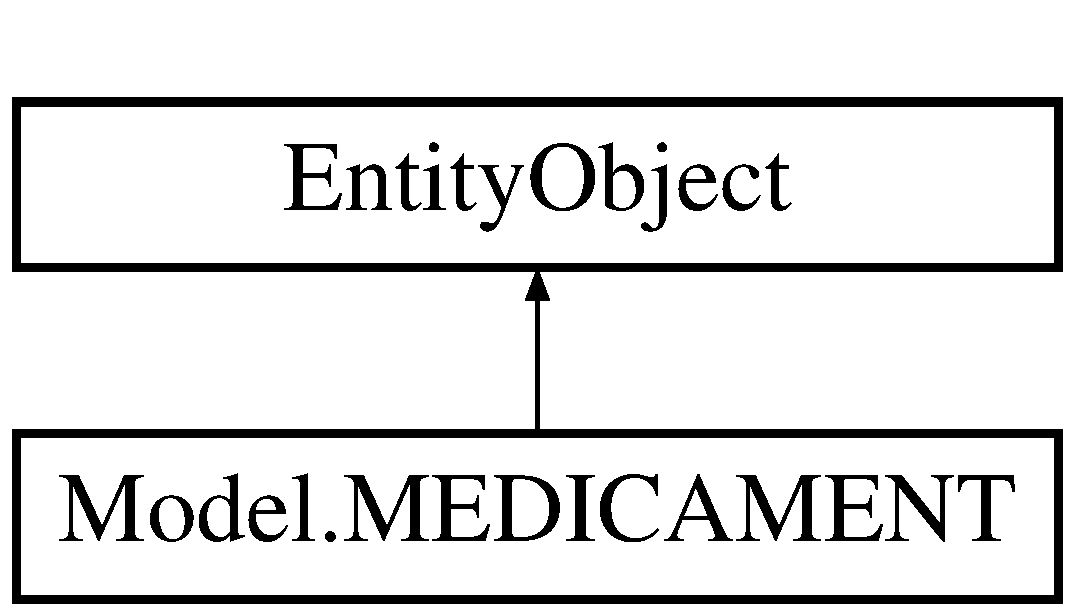
\includegraphics[height=2.000000cm]{class_model_1_1_m_e_d_i_c_a_m_e_n_t}
\end{center}
\end{figure}
\subsection*{Static Public Member Functions}
\begin{DoxyCompactItemize}
\item 
static \hyperlink{class_model_1_1_m_e_d_i_c_a_m_e_n_t}{M\-E\-D\-I\-C\-A\-M\-E\-N\-T} \hyperlink{class_model_1_1_m_e_d_i_c_a_m_e_n_t_a2ca33d05a3c0fb7b7801bf9337b2e511}{Create\-M\-E\-D\-I\-C\-A\-M\-E\-N\-T} (global\-::\-System.\-String \hyperlink{class_model_1_1_m_e_d_i_c_a_m_e_n_t_ad27c0736a77e2ac61cf5d94d7f0ddd00}{depot\-\_\-legal}, global\-::\-System.\-String \hyperlink{class_model_1_1_m_e_d_i_c_a_m_e_n_t_af047e823d0f57ffd36009d48ddae4a9c}{composition}, global\-::\-System.\-String \hyperlink{class_model_1_1_m_e_d_i_c_a_m_e_n_t_ad94a543654340fa8b32a0f82996fb95b}{effet}, global\-::\-System.\-String \hyperlink{class_model_1_1_m_e_d_i_c_a_m_e_n_t_adfdf391b99b65867478accf4a5bb6453}{contreindic}, global\-::\-System.\-Double \hyperlink{class_model_1_1_m_e_d_i_c_a_m_e_n_t_a58b900226ac1992ee6b3f996c667e51a}{prixechantillon})
\begin{DoxyCompactList}\small\item\em Créez un nouvel objet \hyperlink{class_model_1_1_m_e_d_i_c_a_m_e_n_t}{M\-E\-D\-I\-C\-A\-M\-E\-N\-T}. \end{DoxyCompactList}\end{DoxyCompactItemize}
\subsection*{Properties}
\begin{DoxyCompactItemize}
\item 
global\-::\-System.\-String \hyperlink{class_model_1_1_m_e_d_i_c_a_m_e_n_t_ad27c0736a77e2ac61cf5d94d7f0ddd00}{depot\-\_\-legal}\hspace{0.3cm}{\ttfamily  \mbox{[}get, set\mbox{]}}
\begin{DoxyCompactList}\small\item\em Aucune documentation sur les métadonnées n'est disponible. \end{DoxyCompactList}\item 
Nullable$<$ global\-::\-System.\-Int32 $>$ \hyperlink{class_model_1_1_m_e_d_i_c_a_m_e_n_t_a39e97dd11fe652aaa6b30e80694694d3}{code\-\_\-famille}\hspace{0.3cm}{\ttfamily  \mbox{[}get, set\mbox{]}}
\begin{DoxyCompactList}\small\item\em Aucune documentation sur les métadonnées n'est disponible. \end{DoxyCompactList}\item 
Nullable$<$ global\-::\-System.\-Int32 $>$ \hyperlink{class_model_1_1_m_e_d_i_c_a_m_e_n_t_a39501452dd03c0c20690e387a1e4e324}{code\-\_\-present}\hspace{0.3cm}{\ttfamily  \mbox{[}get, set\mbox{]}}
\begin{DoxyCompactList}\small\item\em Aucune documentation sur les métadonnées n'est disponible. \end{DoxyCompactList}\item 
global\-::\-System.\-String \hyperlink{class_model_1_1_m_e_d_i_c_a_m_e_n_t_af047e823d0f57ffd36009d48ddae4a9c}{composition}\hspace{0.3cm}{\ttfamily  \mbox{[}get, set\mbox{]}}
\begin{DoxyCompactList}\small\item\em Aucune documentation sur les métadonnées n'est disponible. \end{DoxyCompactList}\item 
global\-::\-System.\-String \hyperlink{class_model_1_1_m_e_d_i_c_a_m_e_n_t_ad94a543654340fa8b32a0f82996fb95b}{effet}\hspace{0.3cm}{\ttfamily  \mbox{[}get, set\mbox{]}}
\begin{DoxyCompactList}\small\item\em Aucune documentation sur les métadonnées n'est disponible. \end{DoxyCompactList}\item 
global\-::\-System.\-String \hyperlink{class_model_1_1_m_e_d_i_c_a_m_e_n_t_adfdf391b99b65867478accf4a5bb6453}{contreindic}\hspace{0.3cm}{\ttfamily  \mbox{[}get, set\mbox{]}}
\begin{DoxyCompactList}\small\item\em Aucune documentation sur les métadonnées n'est disponible. \end{DoxyCompactList}\item 
global\-::\-System.\-Double \hyperlink{class_model_1_1_m_e_d_i_c_a_m_e_n_t_a58b900226ac1992ee6b3f996c667e51a}{prixechantillon}\hspace{0.3cm}{\ttfamily  \mbox{[}get, set\mbox{]}}
\begin{DoxyCompactList}\small\item\em Aucune documentation sur les métadonnées n'est disponible. \end{DoxyCompactList}\item 
global\-::\-System.\-String \hyperlink{class_model_1_1_m_e_d_i_c_a_m_e_n_t_aac099e9240dac2de02bab20ac675d74b}{nom}\hspace{0.3cm}{\ttfamily  \mbox{[}get, set\mbox{]}}
\begin{DoxyCompactList}\small\item\em Aucune documentation sur les métadonnées n'est disponible. \end{DoxyCompactList}\item 
\hyperlink{class_model_1_1_f_a_m_i_l_l_e}{F\-A\-M\-I\-L\-L\-E} \hyperlink{class_model_1_1_m_e_d_i_c_a_m_e_n_t_aaaa915cc1d5a5956f312da4191f30757}{F\-A\-M\-I\-L\-L\-E}\hspace{0.3cm}{\ttfamily  \mbox{[}get, set\mbox{]}}
\begin{DoxyCompactList}\small\item\em Aucune documentation sur les métadonnées n'est disponible. \end{DoxyCompactList}\item 
Entity\-Reference$<$ \hyperlink{class_model_1_1_f_a_m_i_l_l_e}{F\-A\-M\-I\-L\-L\-E} $>$ \hyperlink{class_model_1_1_m_e_d_i_c_a_m_e_n_t_a9b87fe7d7a3f5819c14257b5b3fb2cb5}{F\-A\-M\-I\-L\-L\-E\-Reference}\hspace{0.3cm}{\ttfamily  \mbox{[}get, set\mbox{]}}
\begin{DoxyCompactList}\small\item\em Aucune documentation sur les métadonnées n'est disponible. \end{DoxyCompactList}\item 
Entity\-Collection$<$ \hyperlink{class_model_1_1_p_r_e_s_c_r_i_r_e}{P\-R\-E\-S\-C\-R\-I\-R\-E} $>$ \hyperlink{class_model_1_1_m_e_d_i_c_a_m_e_n_t_a88b07188c015f24de7f93837eeaa98b1}{P\-R\-E\-S\-C\-R\-I\-R\-E}\hspace{0.3cm}{\ttfamily  \mbox{[}get, set\mbox{]}}
\begin{DoxyCompactList}\small\item\em Aucune documentation sur les métadonnées n'est disponible. \end{DoxyCompactList}\item 
\hyperlink{class_model_1_1_p_r_e_s_e_n_t_a_t_i_o_n}{P\-R\-E\-S\-E\-N\-T\-A\-T\-I\-O\-N} \hyperlink{class_model_1_1_m_e_d_i_c_a_m_e_n_t_a79fed0d0e87a9735a0a0a9f41f6da286}{P\-R\-E\-S\-E\-N\-T\-A\-T\-I\-O\-N}\hspace{0.3cm}{\ttfamily  \mbox{[}get, set\mbox{]}}
\begin{DoxyCompactList}\small\item\em Aucune documentation sur les métadonnées n'est disponible. \end{DoxyCompactList}\item 
Entity\-Reference$<$ \hyperlink{class_model_1_1_p_r_e_s_e_n_t_a_t_i_o_n}{P\-R\-E\-S\-E\-N\-T\-A\-T\-I\-O\-N} $>$ \hyperlink{class_model_1_1_m_e_d_i_c_a_m_e_n_t_a8ee1a7d474625d4c02b7a3145dbfbcf6}{P\-R\-E\-S\-E\-N\-T\-A\-T\-I\-O\-N\-Reference}\hspace{0.3cm}{\ttfamily  \mbox{[}get, set\mbox{]}}
\begin{DoxyCompactList}\small\item\em Aucune documentation sur les métadonnées n'est disponible. \end{DoxyCompactList}\item 
Entity\-Collection$<$ \hyperlink{class_model_1_1_c_o_m_p_o_s_a_n_t}{C\-O\-M\-P\-O\-S\-A\-N\-T} $>$ \hyperlink{class_model_1_1_m_e_d_i_c_a_m_e_n_t_a1faa12602862fab1081752b148f1745b}{C\-O\-M\-P\-O\-S\-A\-N\-T}\hspace{0.3cm}{\ttfamily  \mbox{[}get, set\mbox{]}}
\begin{DoxyCompactList}\small\item\em Aucune documentation sur les métadonnées n'est disponible. \end{DoxyCompactList}\item 
Entity\-Collection$<$ \hyperlink{class_model_1_1_m_e_d_i_c_a_m_e_n_t}{M\-E\-D\-I\-C\-A\-M\-E\-N\-T} $>$ \hyperlink{class_model_1_1_m_e_d_i_c_a_m_e_n_t_a1aa6c5c5d0fb3c9ff49ea59b184b71f7}{M\-E\-D\-I\-C\-A\-M\-E\-N\-T1}\hspace{0.3cm}{\ttfamily  \mbox{[}get, set\mbox{]}}
\begin{DoxyCompactList}\small\item\em Aucune documentation sur les métadonnées n'est disponible. \end{DoxyCompactList}\item 
Entity\-Collection$<$ \hyperlink{class_model_1_1_m_e_d_i_c_a_m_e_n_t}{M\-E\-D\-I\-C\-A\-M\-E\-N\-T} $>$ \hyperlink{class_model_1_1_m_e_d_i_c_a_m_e_n_t_ab27f3343d5bdd58cfb9a866c3163fec3}{M\-E\-D\-I\-C\-A\-M\-E\-N\-T2}\hspace{0.3cm}{\ttfamily  \mbox{[}get, set\mbox{]}}
\begin{DoxyCompactList}\small\item\em Aucune documentation sur les métadonnées n'est disponible. \end{DoxyCompactList}\item 
Entity\-Collection$<$ \hyperlink{class_model_1_1_o_f_f_r_e1}{O\-F\-F\-R\-E1} $>$ \hyperlink{class_model_1_1_m_e_d_i_c_a_m_e_n_t_a54e85fdea163abac71056ffc801917b5}{O\-F\-F\-R\-E}\hspace{0.3cm}{\ttfamily  \mbox{[}get, set\mbox{]}}
\begin{DoxyCompactList}\small\item\em Aucune documentation sur les métadonnées n'est disponible. \end{DoxyCompactList}\item 
Entity\-Collection$<$ \hyperlink{class_model_1_1_p_r_e_s_e_n_t_e}{P\-R\-E\-S\-E\-N\-T\-E} $>$ \hyperlink{class_model_1_1_m_e_d_i_c_a_m_e_n_t_aac80ec949bc5827fed259a383066206d}{P\-R\-E\-S\-E\-N\-T\-E}\hspace{0.3cm}{\ttfamily  \mbox{[}get, set\mbox{]}}
\begin{DoxyCompactList}\small\item\em Aucune documentation sur les métadonnées n'est disponible. \end{DoxyCompactList}\item 
Entity\-Collection$<$ \hyperlink{class_model_1_1_a_v_o_i_r1}{A\-V\-O\-I\-R1} $>$ \hyperlink{class_model_1_1_m_e_d_i_c_a_m_e_n_t_a16a5647738d2faf685e31fa4d4886bda}{A\-V\-O\-I\-R}\hspace{0.3cm}{\ttfamily  \mbox{[}get, set\mbox{]}}
\begin{DoxyCompactList}\small\item\em Aucune documentation sur les métadonnées n'est disponible. \end{DoxyCompactList}\end{DoxyCompactItemize}


\subsection{Detailed Description}
Aucune documentation sur les métadonnées n'est disponible. 



\subsection{Member Function Documentation}
\hypertarget{class_model_1_1_m_e_d_i_c_a_m_e_n_t_a2ca33d05a3c0fb7b7801bf9337b2e511}{\index{Model\-::\-M\-E\-D\-I\-C\-A\-M\-E\-N\-T@{Model\-::\-M\-E\-D\-I\-C\-A\-M\-E\-N\-T}!Create\-M\-E\-D\-I\-C\-A\-M\-E\-N\-T@{Create\-M\-E\-D\-I\-C\-A\-M\-E\-N\-T}}
\index{Create\-M\-E\-D\-I\-C\-A\-M\-E\-N\-T@{Create\-M\-E\-D\-I\-C\-A\-M\-E\-N\-T}!Model::MEDICAMENT@{Model\-::\-M\-E\-D\-I\-C\-A\-M\-E\-N\-T}}
\subsubsection[{Create\-M\-E\-D\-I\-C\-A\-M\-E\-N\-T}]{\setlength{\rightskip}{0pt plus 5cm}static {\bf M\-E\-D\-I\-C\-A\-M\-E\-N\-T} Model.\-M\-E\-D\-I\-C\-A\-M\-E\-N\-T.\-Create\-M\-E\-D\-I\-C\-A\-M\-E\-N\-T (
\begin{DoxyParamCaption}
\item[{global\-::\-System.\-String}]{depot\-\_\-legal, }
\item[{global\-::\-System.\-String}]{composition, }
\item[{global\-::\-System.\-String}]{effet, }
\item[{global\-::\-System.\-String}]{contreindic, }
\item[{global\-::\-System.\-Double}]{prixechantillon}
\end{DoxyParamCaption}
)\hspace{0.3cm}{\ttfamily [static]}}}\label{class_model_1_1_m_e_d_i_c_a_m_e_n_t_a2ca33d05a3c0fb7b7801bf9337b2e511}


Créez un nouvel objet \hyperlink{class_model_1_1_m_e_d_i_c_a_m_e_n_t}{M\-E\-D\-I\-C\-A\-M\-E\-N\-T}. 


\begin{DoxyParams}{Parameters}
{\em depot\-\_\-legal} & Valeur initiale de la propriété depot\-\_\-legal.\\
\hline
{\em composition} & Valeur initiale de la propriété composition.\\
\hline
{\em effet} & Valeur initiale de la propriété effet.\\
\hline
{\em contreindic} & Valeur initiale de la propriété contreindic.\\
\hline
{\em prixechantillon} & Valeur initiale de la propriété prixechantillon.\\
\hline
\end{DoxyParams}


\subsection{Property Documentation}
\hypertarget{class_model_1_1_m_e_d_i_c_a_m_e_n_t_a16a5647738d2faf685e31fa4d4886bda}{\index{Model\-::\-M\-E\-D\-I\-C\-A\-M\-E\-N\-T@{Model\-::\-M\-E\-D\-I\-C\-A\-M\-E\-N\-T}!A\-V\-O\-I\-R@{A\-V\-O\-I\-R}}
\index{A\-V\-O\-I\-R@{A\-V\-O\-I\-R}!Model::MEDICAMENT@{Model\-::\-M\-E\-D\-I\-C\-A\-M\-E\-N\-T}}
\subsubsection[{A\-V\-O\-I\-R}]{\setlength{\rightskip}{0pt plus 5cm}Entity\-Collection$<${\bf A\-V\-O\-I\-R1}$>$ Model.\-M\-E\-D\-I\-C\-A\-M\-E\-N\-T.\-A\-V\-O\-I\-R\hspace{0.3cm}{\ttfamily [get]}, {\ttfamily [set]}}}\label{class_model_1_1_m_e_d_i_c_a_m_e_n_t_a16a5647738d2faf685e31fa4d4886bda}


Aucune documentation sur les métadonnées n'est disponible. 

\hypertarget{class_model_1_1_m_e_d_i_c_a_m_e_n_t_a39e97dd11fe652aaa6b30e80694694d3}{\index{Model\-::\-M\-E\-D\-I\-C\-A\-M\-E\-N\-T@{Model\-::\-M\-E\-D\-I\-C\-A\-M\-E\-N\-T}!code\-\_\-famille@{code\-\_\-famille}}
\index{code\-\_\-famille@{code\-\_\-famille}!Model::MEDICAMENT@{Model\-::\-M\-E\-D\-I\-C\-A\-M\-E\-N\-T}}
\subsubsection[{code\-\_\-famille}]{\setlength{\rightskip}{0pt plus 5cm}Nullable$<$global.\-System.\-Int32$>$ Model.\-M\-E\-D\-I\-C\-A\-M\-E\-N\-T.\-code\-\_\-famille\hspace{0.3cm}{\ttfamily [get]}, {\ttfamily [set]}}}\label{class_model_1_1_m_e_d_i_c_a_m_e_n_t_a39e97dd11fe652aaa6b30e80694694d3}


Aucune documentation sur les métadonnées n'est disponible. 

\hypertarget{class_model_1_1_m_e_d_i_c_a_m_e_n_t_a39501452dd03c0c20690e387a1e4e324}{\index{Model\-::\-M\-E\-D\-I\-C\-A\-M\-E\-N\-T@{Model\-::\-M\-E\-D\-I\-C\-A\-M\-E\-N\-T}!code\-\_\-present@{code\-\_\-present}}
\index{code\-\_\-present@{code\-\_\-present}!Model::MEDICAMENT@{Model\-::\-M\-E\-D\-I\-C\-A\-M\-E\-N\-T}}
\subsubsection[{code\-\_\-present}]{\setlength{\rightskip}{0pt plus 5cm}Nullable$<$global.\-System.\-Int32$>$ Model.\-M\-E\-D\-I\-C\-A\-M\-E\-N\-T.\-code\-\_\-present\hspace{0.3cm}{\ttfamily [get]}, {\ttfamily [set]}}}\label{class_model_1_1_m_e_d_i_c_a_m_e_n_t_a39501452dd03c0c20690e387a1e4e324}


Aucune documentation sur les métadonnées n'est disponible. 

\hypertarget{class_model_1_1_m_e_d_i_c_a_m_e_n_t_a1faa12602862fab1081752b148f1745b}{\index{Model\-::\-M\-E\-D\-I\-C\-A\-M\-E\-N\-T@{Model\-::\-M\-E\-D\-I\-C\-A\-M\-E\-N\-T}!C\-O\-M\-P\-O\-S\-A\-N\-T@{C\-O\-M\-P\-O\-S\-A\-N\-T}}
\index{C\-O\-M\-P\-O\-S\-A\-N\-T@{C\-O\-M\-P\-O\-S\-A\-N\-T}!Model::MEDICAMENT@{Model\-::\-M\-E\-D\-I\-C\-A\-M\-E\-N\-T}}
\subsubsection[{C\-O\-M\-P\-O\-S\-A\-N\-T}]{\setlength{\rightskip}{0pt plus 5cm}Entity\-Collection$<${\bf C\-O\-M\-P\-O\-S\-A\-N\-T}$>$ Model.\-M\-E\-D\-I\-C\-A\-M\-E\-N\-T.\-C\-O\-M\-P\-O\-S\-A\-N\-T\hspace{0.3cm}{\ttfamily [get]}, {\ttfamily [set]}}}\label{class_model_1_1_m_e_d_i_c_a_m_e_n_t_a1faa12602862fab1081752b148f1745b}


Aucune documentation sur les métadonnées n'est disponible. 

\hypertarget{class_model_1_1_m_e_d_i_c_a_m_e_n_t_af047e823d0f57ffd36009d48ddae4a9c}{\index{Model\-::\-M\-E\-D\-I\-C\-A\-M\-E\-N\-T@{Model\-::\-M\-E\-D\-I\-C\-A\-M\-E\-N\-T}!composition@{composition}}
\index{composition@{composition}!Model::MEDICAMENT@{Model\-::\-M\-E\-D\-I\-C\-A\-M\-E\-N\-T}}
\subsubsection[{composition}]{\setlength{\rightskip}{0pt plus 5cm}global.\-System.\-String Model.\-M\-E\-D\-I\-C\-A\-M\-E\-N\-T.\-composition\hspace{0.3cm}{\ttfamily [get]}, {\ttfamily [set]}}}\label{class_model_1_1_m_e_d_i_c_a_m_e_n_t_af047e823d0f57ffd36009d48ddae4a9c}


Aucune documentation sur les métadonnées n'est disponible. 

\hypertarget{class_model_1_1_m_e_d_i_c_a_m_e_n_t_adfdf391b99b65867478accf4a5bb6453}{\index{Model\-::\-M\-E\-D\-I\-C\-A\-M\-E\-N\-T@{Model\-::\-M\-E\-D\-I\-C\-A\-M\-E\-N\-T}!contreindic@{contreindic}}
\index{contreindic@{contreindic}!Model::MEDICAMENT@{Model\-::\-M\-E\-D\-I\-C\-A\-M\-E\-N\-T}}
\subsubsection[{contreindic}]{\setlength{\rightskip}{0pt plus 5cm}global.\-System.\-String Model.\-M\-E\-D\-I\-C\-A\-M\-E\-N\-T.\-contreindic\hspace{0.3cm}{\ttfamily [get]}, {\ttfamily [set]}}}\label{class_model_1_1_m_e_d_i_c_a_m_e_n_t_adfdf391b99b65867478accf4a5bb6453}


Aucune documentation sur les métadonnées n'est disponible. 

\hypertarget{class_model_1_1_m_e_d_i_c_a_m_e_n_t_ad27c0736a77e2ac61cf5d94d7f0ddd00}{\index{Model\-::\-M\-E\-D\-I\-C\-A\-M\-E\-N\-T@{Model\-::\-M\-E\-D\-I\-C\-A\-M\-E\-N\-T}!depot\-\_\-legal@{depot\-\_\-legal}}
\index{depot\-\_\-legal@{depot\-\_\-legal}!Model::MEDICAMENT@{Model\-::\-M\-E\-D\-I\-C\-A\-M\-E\-N\-T}}
\subsubsection[{depot\-\_\-legal}]{\setlength{\rightskip}{0pt plus 5cm}global.\-System.\-String Model.\-M\-E\-D\-I\-C\-A\-M\-E\-N\-T.\-depot\-\_\-legal\hspace{0.3cm}{\ttfamily [get]}, {\ttfamily [set]}}}\label{class_model_1_1_m_e_d_i_c_a_m_e_n_t_ad27c0736a77e2ac61cf5d94d7f0ddd00}


Aucune documentation sur les métadonnées n'est disponible. 

\hypertarget{class_model_1_1_m_e_d_i_c_a_m_e_n_t_ad94a543654340fa8b32a0f82996fb95b}{\index{Model\-::\-M\-E\-D\-I\-C\-A\-M\-E\-N\-T@{Model\-::\-M\-E\-D\-I\-C\-A\-M\-E\-N\-T}!effet@{effet}}
\index{effet@{effet}!Model::MEDICAMENT@{Model\-::\-M\-E\-D\-I\-C\-A\-M\-E\-N\-T}}
\subsubsection[{effet}]{\setlength{\rightskip}{0pt plus 5cm}global.\-System.\-String Model.\-M\-E\-D\-I\-C\-A\-M\-E\-N\-T.\-effet\hspace{0.3cm}{\ttfamily [get]}, {\ttfamily [set]}}}\label{class_model_1_1_m_e_d_i_c_a_m_e_n_t_ad94a543654340fa8b32a0f82996fb95b}


Aucune documentation sur les métadonnées n'est disponible. 

\hypertarget{class_model_1_1_m_e_d_i_c_a_m_e_n_t_aaaa915cc1d5a5956f312da4191f30757}{\index{Model\-::\-M\-E\-D\-I\-C\-A\-M\-E\-N\-T@{Model\-::\-M\-E\-D\-I\-C\-A\-M\-E\-N\-T}!F\-A\-M\-I\-L\-L\-E@{F\-A\-M\-I\-L\-L\-E}}
\index{F\-A\-M\-I\-L\-L\-E@{F\-A\-M\-I\-L\-L\-E}!Model::MEDICAMENT@{Model\-::\-M\-E\-D\-I\-C\-A\-M\-E\-N\-T}}
\subsubsection[{F\-A\-M\-I\-L\-L\-E}]{\setlength{\rightskip}{0pt plus 5cm}{\bf F\-A\-M\-I\-L\-L\-E} Model.\-M\-E\-D\-I\-C\-A\-M\-E\-N\-T.\-F\-A\-M\-I\-L\-L\-E\hspace{0.3cm}{\ttfamily [get]}, {\ttfamily [set]}}}\label{class_model_1_1_m_e_d_i_c_a_m_e_n_t_aaaa915cc1d5a5956f312da4191f30757}


Aucune documentation sur les métadonnées n'est disponible. 

\hypertarget{class_model_1_1_m_e_d_i_c_a_m_e_n_t_a9b87fe7d7a3f5819c14257b5b3fb2cb5}{\index{Model\-::\-M\-E\-D\-I\-C\-A\-M\-E\-N\-T@{Model\-::\-M\-E\-D\-I\-C\-A\-M\-E\-N\-T}!F\-A\-M\-I\-L\-L\-E\-Reference@{F\-A\-M\-I\-L\-L\-E\-Reference}}
\index{F\-A\-M\-I\-L\-L\-E\-Reference@{F\-A\-M\-I\-L\-L\-E\-Reference}!Model::MEDICAMENT@{Model\-::\-M\-E\-D\-I\-C\-A\-M\-E\-N\-T}}
\subsubsection[{F\-A\-M\-I\-L\-L\-E\-Reference}]{\setlength{\rightskip}{0pt plus 5cm}Entity\-Reference$<${\bf F\-A\-M\-I\-L\-L\-E}$>$ Model.\-M\-E\-D\-I\-C\-A\-M\-E\-N\-T.\-F\-A\-M\-I\-L\-L\-E\-Reference\hspace{0.3cm}{\ttfamily [get]}, {\ttfamily [set]}}}\label{class_model_1_1_m_e_d_i_c_a_m_e_n_t_a9b87fe7d7a3f5819c14257b5b3fb2cb5}


Aucune documentation sur les métadonnées n'est disponible. 

\hypertarget{class_model_1_1_m_e_d_i_c_a_m_e_n_t_a1aa6c5c5d0fb3c9ff49ea59b184b71f7}{\index{Model\-::\-M\-E\-D\-I\-C\-A\-M\-E\-N\-T@{Model\-::\-M\-E\-D\-I\-C\-A\-M\-E\-N\-T}!M\-E\-D\-I\-C\-A\-M\-E\-N\-T1@{M\-E\-D\-I\-C\-A\-M\-E\-N\-T1}}
\index{M\-E\-D\-I\-C\-A\-M\-E\-N\-T1@{M\-E\-D\-I\-C\-A\-M\-E\-N\-T1}!Model::MEDICAMENT@{Model\-::\-M\-E\-D\-I\-C\-A\-M\-E\-N\-T}}
\subsubsection[{M\-E\-D\-I\-C\-A\-M\-E\-N\-T1}]{\setlength{\rightskip}{0pt plus 5cm}Entity\-Collection$<${\bf M\-E\-D\-I\-C\-A\-M\-E\-N\-T}$>$ Model.\-M\-E\-D\-I\-C\-A\-M\-E\-N\-T.\-M\-E\-D\-I\-C\-A\-M\-E\-N\-T1\hspace{0.3cm}{\ttfamily [get]}, {\ttfamily [set]}}}\label{class_model_1_1_m_e_d_i_c_a_m_e_n_t_a1aa6c5c5d0fb3c9ff49ea59b184b71f7}


Aucune documentation sur les métadonnées n'est disponible. 

\hypertarget{class_model_1_1_m_e_d_i_c_a_m_e_n_t_ab27f3343d5bdd58cfb9a866c3163fec3}{\index{Model\-::\-M\-E\-D\-I\-C\-A\-M\-E\-N\-T@{Model\-::\-M\-E\-D\-I\-C\-A\-M\-E\-N\-T}!M\-E\-D\-I\-C\-A\-M\-E\-N\-T2@{M\-E\-D\-I\-C\-A\-M\-E\-N\-T2}}
\index{M\-E\-D\-I\-C\-A\-M\-E\-N\-T2@{M\-E\-D\-I\-C\-A\-M\-E\-N\-T2}!Model::MEDICAMENT@{Model\-::\-M\-E\-D\-I\-C\-A\-M\-E\-N\-T}}
\subsubsection[{M\-E\-D\-I\-C\-A\-M\-E\-N\-T2}]{\setlength{\rightskip}{0pt plus 5cm}Entity\-Collection$<${\bf M\-E\-D\-I\-C\-A\-M\-E\-N\-T}$>$ Model.\-M\-E\-D\-I\-C\-A\-M\-E\-N\-T.\-M\-E\-D\-I\-C\-A\-M\-E\-N\-T2\hspace{0.3cm}{\ttfamily [get]}, {\ttfamily [set]}}}\label{class_model_1_1_m_e_d_i_c_a_m_e_n_t_ab27f3343d5bdd58cfb9a866c3163fec3}


Aucune documentation sur les métadonnées n'est disponible. 

\hypertarget{class_model_1_1_m_e_d_i_c_a_m_e_n_t_aac099e9240dac2de02bab20ac675d74b}{\index{Model\-::\-M\-E\-D\-I\-C\-A\-M\-E\-N\-T@{Model\-::\-M\-E\-D\-I\-C\-A\-M\-E\-N\-T}!nom@{nom}}
\index{nom@{nom}!Model::MEDICAMENT@{Model\-::\-M\-E\-D\-I\-C\-A\-M\-E\-N\-T}}
\subsubsection[{nom}]{\setlength{\rightskip}{0pt plus 5cm}global.\-System.\-String Model.\-M\-E\-D\-I\-C\-A\-M\-E\-N\-T.\-nom\hspace{0.3cm}{\ttfamily [get]}, {\ttfamily [set]}}}\label{class_model_1_1_m_e_d_i_c_a_m_e_n_t_aac099e9240dac2de02bab20ac675d74b}


Aucune documentation sur les métadonnées n'est disponible. 

\hypertarget{class_model_1_1_m_e_d_i_c_a_m_e_n_t_a54e85fdea163abac71056ffc801917b5}{\index{Model\-::\-M\-E\-D\-I\-C\-A\-M\-E\-N\-T@{Model\-::\-M\-E\-D\-I\-C\-A\-M\-E\-N\-T}!O\-F\-F\-R\-E@{O\-F\-F\-R\-E}}
\index{O\-F\-F\-R\-E@{O\-F\-F\-R\-E}!Model::MEDICAMENT@{Model\-::\-M\-E\-D\-I\-C\-A\-M\-E\-N\-T}}
\subsubsection[{O\-F\-F\-R\-E}]{\setlength{\rightskip}{0pt plus 5cm}Entity\-Collection$<${\bf O\-F\-F\-R\-E1}$>$ Model.\-M\-E\-D\-I\-C\-A\-M\-E\-N\-T.\-O\-F\-F\-R\-E\hspace{0.3cm}{\ttfamily [get]}, {\ttfamily [set]}}}\label{class_model_1_1_m_e_d_i_c_a_m_e_n_t_a54e85fdea163abac71056ffc801917b5}


Aucune documentation sur les métadonnées n'est disponible. 

\hypertarget{class_model_1_1_m_e_d_i_c_a_m_e_n_t_a88b07188c015f24de7f93837eeaa98b1}{\index{Model\-::\-M\-E\-D\-I\-C\-A\-M\-E\-N\-T@{Model\-::\-M\-E\-D\-I\-C\-A\-M\-E\-N\-T}!P\-R\-E\-S\-C\-R\-I\-R\-E@{P\-R\-E\-S\-C\-R\-I\-R\-E}}
\index{P\-R\-E\-S\-C\-R\-I\-R\-E@{P\-R\-E\-S\-C\-R\-I\-R\-E}!Model::MEDICAMENT@{Model\-::\-M\-E\-D\-I\-C\-A\-M\-E\-N\-T}}
\subsubsection[{P\-R\-E\-S\-C\-R\-I\-R\-E}]{\setlength{\rightskip}{0pt plus 5cm}Entity\-Collection$<${\bf P\-R\-E\-S\-C\-R\-I\-R\-E}$>$ Model.\-M\-E\-D\-I\-C\-A\-M\-E\-N\-T.\-P\-R\-E\-S\-C\-R\-I\-R\-E\hspace{0.3cm}{\ttfamily [get]}, {\ttfamily [set]}}}\label{class_model_1_1_m_e_d_i_c_a_m_e_n_t_a88b07188c015f24de7f93837eeaa98b1}


Aucune documentation sur les métadonnées n'est disponible. 

\hypertarget{class_model_1_1_m_e_d_i_c_a_m_e_n_t_a79fed0d0e87a9735a0a0a9f41f6da286}{\index{Model\-::\-M\-E\-D\-I\-C\-A\-M\-E\-N\-T@{Model\-::\-M\-E\-D\-I\-C\-A\-M\-E\-N\-T}!P\-R\-E\-S\-E\-N\-T\-A\-T\-I\-O\-N@{P\-R\-E\-S\-E\-N\-T\-A\-T\-I\-O\-N}}
\index{P\-R\-E\-S\-E\-N\-T\-A\-T\-I\-O\-N@{P\-R\-E\-S\-E\-N\-T\-A\-T\-I\-O\-N}!Model::MEDICAMENT@{Model\-::\-M\-E\-D\-I\-C\-A\-M\-E\-N\-T}}
\subsubsection[{P\-R\-E\-S\-E\-N\-T\-A\-T\-I\-O\-N}]{\setlength{\rightskip}{0pt plus 5cm}{\bf P\-R\-E\-S\-E\-N\-T\-A\-T\-I\-O\-N} Model.\-M\-E\-D\-I\-C\-A\-M\-E\-N\-T.\-P\-R\-E\-S\-E\-N\-T\-A\-T\-I\-O\-N\hspace{0.3cm}{\ttfamily [get]}, {\ttfamily [set]}}}\label{class_model_1_1_m_e_d_i_c_a_m_e_n_t_a79fed0d0e87a9735a0a0a9f41f6da286}


Aucune documentation sur les métadonnées n'est disponible. 

\hypertarget{class_model_1_1_m_e_d_i_c_a_m_e_n_t_a8ee1a7d474625d4c02b7a3145dbfbcf6}{\index{Model\-::\-M\-E\-D\-I\-C\-A\-M\-E\-N\-T@{Model\-::\-M\-E\-D\-I\-C\-A\-M\-E\-N\-T}!P\-R\-E\-S\-E\-N\-T\-A\-T\-I\-O\-N\-Reference@{P\-R\-E\-S\-E\-N\-T\-A\-T\-I\-O\-N\-Reference}}
\index{P\-R\-E\-S\-E\-N\-T\-A\-T\-I\-O\-N\-Reference@{P\-R\-E\-S\-E\-N\-T\-A\-T\-I\-O\-N\-Reference}!Model::MEDICAMENT@{Model\-::\-M\-E\-D\-I\-C\-A\-M\-E\-N\-T}}
\subsubsection[{P\-R\-E\-S\-E\-N\-T\-A\-T\-I\-O\-N\-Reference}]{\setlength{\rightskip}{0pt plus 5cm}Entity\-Reference$<${\bf P\-R\-E\-S\-E\-N\-T\-A\-T\-I\-O\-N}$>$ Model.\-M\-E\-D\-I\-C\-A\-M\-E\-N\-T.\-P\-R\-E\-S\-E\-N\-T\-A\-T\-I\-O\-N\-Reference\hspace{0.3cm}{\ttfamily [get]}, {\ttfamily [set]}}}\label{class_model_1_1_m_e_d_i_c_a_m_e_n_t_a8ee1a7d474625d4c02b7a3145dbfbcf6}


Aucune documentation sur les métadonnées n'est disponible. 

\hypertarget{class_model_1_1_m_e_d_i_c_a_m_e_n_t_aac80ec949bc5827fed259a383066206d}{\index{Model\-::\-M\-E\-D\-I\-C\-A\-M\-E\-N\-T@{Model\-::\-M\-E\-D\-I\-C\-A\-M\-E\-N\-T}!P\-R\-E\-S\-E\-N\-T\-E@{P\-R\-E\-S\-E\-N\-T\-E}}
\index{P\-R\-E\-S\-E\-N\-T\-E@{P\-R\-E\-S\-E\-N\-T\-E}!Model::MEDICAMENT@{Model\-::\-M\-E\-D\-I\-C\-A\-M\-E\-N\-T}}
\subsubsection[{P\-R\-E\-S\-E\-N\-T\-E}]{\setlength{\rightskip}{0pt plus 5cm}Entity\-Collection$<${\bf P\-R\-E\-S\-E\-N\-T\-E}$>$ Model.\-M\-E\-D\-I\-C\-A\-M\-E\-N\-T.\-P\-R\-E\-S\-E\-N\-T\-E\hspace{0.3cm}{\ttfamily [get]}, {\ttfamily [set]}}}\label{class_model_1_1_m_e_d_i_c_a_m_e_n_t_aac80ec949bc5827fed259a383066206d}


Aucune documentation sur les métadonnées n'est disponible. 

\hypertarget{class_model_1_1_m_e_d_i_c_a_m_e_n_t_a58b900226ac1992ee6b3f996c667e51a}{\index{Model\-::\-M\-E\-D\-I\-C\-A\-M\-E\-N\-T@{Model\-::\-M\-E\-D\-I\-C\-A\-M\-E\-N\-T}!prixechantillon@{prixechantillon}}
\index{prixechantillon@{prixechantillon}!Model::MEDICAMENT@{Model\-::\-M\-E\-D\-I\-C\-A\-M\-E\-N\-T}}
\subsubsection[{prixechantillon}]{\setlength{\rightskip}{0pt plus 5cm}global.\-System.\-Double Model.\-M\-E\-D\-I\-C\-A\-M\-E\-N\-T.\-prixechantillon\hspace{0.3cm}{\ttfamily [get]}, {\ttfamily [set]}}}\label{class_model_1_1_m_e_d_i_c_a_m_e_n_t_a58b900226ac1992ee6b3f996c667e51a}


Aucune documentation sur les métadonnées n'est disponible. 



The documentation for this class was generated from the following file\-:\begin{DoxyCompactItemize}
\item 
C\-:/\-Users/dju/\-Documents/\-Visual Studio 2012/\-Projects/\-P\-P\-E/\-P\-P\-E3/\-Model/\hyperlink{_model_bdd_sio_8_designer_8cs}{Model\-Bdd\-Sio.\-Designer.\-cs}\end{DoxyCompactItemize}

\hypertarget{class_model_1_1_m_o_t_i_f}{\section{Model.\-M\-O\-T\-I\-F Class Reference}
\label{class_model_1_1_m_o_t_i_f}\index{Model.\-M\-O\-T\-I\-F@{Model.\-M\-O\-T\-I\-F}}
}


Aucune documentation sur les métadonnées n'est disponible.  


Inheritance diagram for Model.\-M\-O\-T\-I\-F\-:\begin{figure}[H]
\begin{center}
\leavevmode
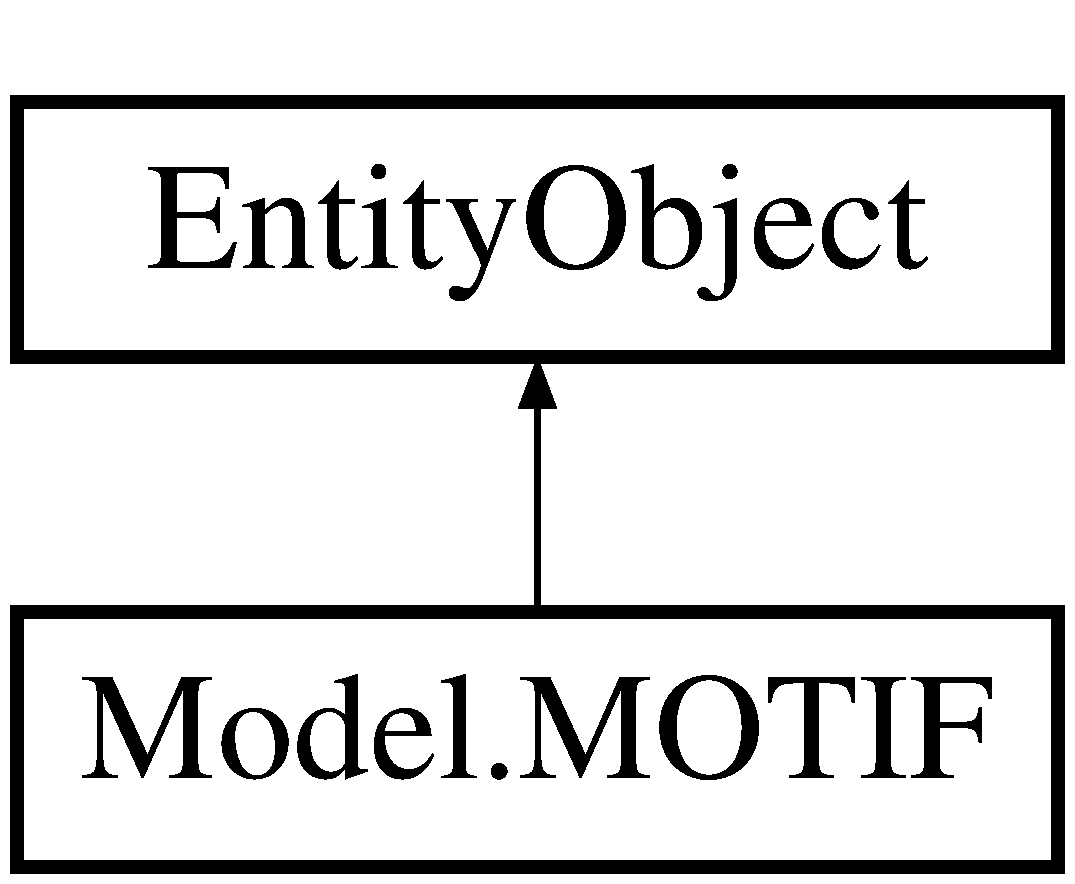
\includegraphics[height=2.000000cm]{class_model_1_1_m_o_t_i_f}
\end{center}
\end{figure}
\subsection*{Static Public Member Functions}
\begin{DoxyCompactItemize}
\item 
static \hyperlink{class_model_1_1_m_o_t_i_f}{M\-O\-T\-I\-F} \hyperlink{class_model_1_1_m_o_t_i_f_a0a7644d2e98b8191ea1b65d8a5500c9b}{Create\-M\-O\-T\-I\-F} (global\-::\-System.\-Int32 \hyperlink{class_model_1_1_m_o_t_i_f_a72c3259738d73e8c4ab96d046c7fd5a9}{code\-\_\-motif}, global\-::\-System.\-String \hyperlink{class_model_1_1_m_o_t_i_f_a72046bb40be3fd2da573e935fb49a81b}{libelle\-\_\-motif})
\begin{DoxyCompactList}\small\item\em Créez un nouvel objet \hyperlink{class_model_1_1_m_o_t_i_f}{M\-O\-T\-I\-F}. \end{DoxyCompactList}\end{DoxyCompactItemize}
\subsection*{Properties}
\begin{DoxyCompactItemize}
\item 
global\-::\-System.\-Int32 \hyperlink{class_model_1_1_m_o_t_i_f_a72c3259738d73e8c4ab96d046c7fd5a9}{code\-\_\-motif}\hspace{0.3cm}{\ttfamily  \mbox{[}get, set\mbox{]}}
\begin{DoxyCompactList}\small\item\em Aucune documentation sur les métadonnées n'est disponible. \end{DoxyCompactList}\item 
global\-::\-System.\-String \hyperlink{class_model_1_1_m_o_t_i_f_a72046bb40be3fd2da573e935fb49a81b}{libelle\-\_\-motif}\hspace{0.3cm}{\ttfamily  \mbox{[}get, set\mbox{]}}
\begin{DoxyCompactList}\small\item\em Aucune documentation sur les métadonnées n'est disponible. \end{DoxyCompactList}\item 
Entity\-Collection\\*
$<$ \hyperlink{class_model_1_1_r_a_p_p_o_r_t___d_e___v_i_s_i_t_e}{R\-A\-P\-P\-O\-R\-T\-\_\-\-D\-E\-\_\-\-V\-I\-S\-I\-T\-E} $>$ \hyperlink{class_model_1_1_m_o_t_i_f_a274a1b2205178e4d10d4facee7b4653b}{R\-A\-P\-P\-O\-R\-T\-\_\-\-D\-E\-\_\-\-V\-I\-S\-I\-T\-E}\hspace{0.3cm}{\ttfamily  \mbox{[}get, set\mbox{]}}
\begin{DoxyCompactList}\small\item\em Aucune documentation sur les métadonnées n'est disponible. \end{DoxyCompactList}\end{DoxyCompactItemize}


\subsection{Detailed Description}
Aucune documentation sur les métadonnées n'est disponible. 



\subsection{Member Function Documentation}
\hypertarget{class_model_1_1_m_o_t_i_f_a0a7644d2e98b8191ea1b65d8a5500c9b}{\index{Model\-::\-M\-O\-T\-I\-F@{Model\-::\-M\-O\-T\-I\-F}!Create\-M\-O\-T\-I\-F@{Create\-M\-O\-T\-I\-F}}
\index{Create\-M\-O\-T\-I\-F@{Create\-M\-O\-T\-I\-F}!Model::MOTIF@{Model\-::\-M\-O\-T\-I\-F}}
\subsubsection[{Create\-M\-O\-T\-I\-F}]{\setlength{\rightskip}{0pt plus 5cm}static {\bf M\-O\-T\-I\-F} Model.\-M\-O\-T\-I\-F.\-Create\-M\-O\-T\-I\-F (
\begin{DoxyParamCaption}
\item[{global\-::\-System.\-Int32}]{code\-\_\-motif, }
\item[{global\-::\-System.\-String}]{libelle\-\_\-motif}
\end{DoxyParamCaption}
)\hspace{0.3cm}{\ttfamily [static]}}}\label{class_model_1_1_m_o_t_i_f_a0a7644d2e98b8191ea1b65d8a5500c9b}


Créez un nouvel objet \hyperlink{class_model_1_1_m_o_t_i_f}{M\-O\-T\-I\-F}. 


\begin{DoxyParams}{Parameters}
{\em code\-\_\-motif} & Valeur initiale de la propriété code\-\_\-motif.\\
\hline
{\em libelle\-\_\-motif} & Valeur initiale de la propriété libelle\-\_\-motif.\\
\hline
\end{DoxyParams}


\subsection{Property Documentation}
\hypertarget{class_model_1_1_m_o_t_i_f_a72c3259738d73e8c4ab96d046c7fd5a9}{\index{Model\-::\-M\-O\-T\-I\-F@{Model\-::\-M\-O\-T\-I\-F}!code\-\_\-motif@{code\-\_\-motif}}
\index{code\-\_\-motif@{code\-\_\-motif}!Model::MOTIF@{Model\-::\-M\-O\-T\-I\-F}}
\subsubsection[{code\-\_\-motif}]{\setlength{\rightskip}{0pt plus 5cm}global.\-System.\-Int32 Model.\-M\-O\-T\-I\-F.\-code\-\_\-motif\hspace{0.3cm}{\ttfamily [get]}, {\ttfamily [set]}}}\label{class_model_1_1_m_o_t_i_f_a72c3259738d73e8c4ab96d046c7fd5a9}


Aucune documentation sur les métadonnées n'est disponible. 

\hypertarget{class_model_1_1_m_o_t_i_f_a72046bb40be3fd2da573e935fb49a81b}{\index{Model\-::\-M\-O\-T\-I\-F@{Model\-::\-M\-O\-T\-I\-F}!libelle\-\_\-motif@{libelle\-\_\-motif}}
\index{libelle\-\_\-motif@{libelle\-\_\-motif}!Model::MOTIF@{Model\-::\-M\-O\-T\-I\-F}}
\subsubsection[{libelle\-\_\-motif}]{\setlength{\rightskip}{0pt plus 5cm}global.\-System.\-String Model.\-M\-O\-T\-I\-F.\-libelle\-\_\-motif\hspace{0.3cm}{\ttfamily [get]}, {\ttfamily [set]}}}\label{class_model_1_1_m_o_t_i_f_a72046bb40be3fd2da573e935fb49a81b}


Aucune documentation sur les métadonnées n'est disponible. 

\hypertarget{class_model_1_1_m_o_t_i_f_a274a1b2205178e4d10d4facee7b4653b}{\index{Model\-::\-M\-O\-T\-I\-F@{Model\-::\-M\-O\-T\-I\-F}!R\-A\-P\-P\-O\-R\-T\-\_\-\-D\-E\-\_\-\-V\-I\-S\-I\-T\-E@{R\-A\-P\-P\-O\-R\-T\-\_\-\-D\-E\-\_\-\-V\-I\-S\-I\-T\-E}}
\index{R\-A\-P\-P\-O\-R\-T\-\_\-\-D\-E\-\_\-\-V\-I\-S\-I\-T\-E@{R\-A\-P\-P\-O\-R\-T\-\_\-\-D\-E\-\_\-\-V\-I\-S\-I\-T\-E}!Model::MOTIF@{Model\-::\-M\-O\-T\-I\-F}}
\subsubsection[{R\-A\-P\-P\-O\-R\-T\-\_\-\-D\-E\-\_\-\-V\-I\-S\-I\-T\-E}]{\setlength{\rightskip}{0pt plus 5cm}Entity\-Collection$<${\bf R\-A\-P\-P\-O\-R\-T\-\_\-\-D\-E\-\_\-\-V\-I\-S\-I\-T\-E}$>$ Model.\-M\-O\-T\-I\-F.\-R\-A\-P\-P\-O\-R\-T\-\_\-\-D\-E\-\_\-\-V\-I\-S\-I\-T\-E\hspace{0.3cm}{\ttfamily [get]}, {\ttfamily [set]}}}\label{class_model_1_1_m_o_t_i_f_a274a1b2205178e4d10d4facee7b4653b}


Aucune documentation sur les métadonnées n'est disponible. 



The documentation for this class was generated from the following file\-:\begin{DoxyCompactItemize}
\item 
C\-:/\-Users/dju/\-Documents/\-Visual Studio 2012/\-Projects/\-P\-P\-E/\-P\-P\-E3/\-Model/\hyperlink{_model_bdd_sio_8_designer_8cs}{Model\-Bdd\-Sio.\-Designer.\-cs}\end{DoxyCompactItemize}

\hypertarget{class_wpf_application_1_1_helpers_1_1_notification_object}{\section{Wpf\-Application.\-Helpers.\-Notification\-Object Class Reference}
\label{class_wpf_application_1_1_helpers_1_1_notification_object}\index{Wpf\-Application.\-Helpers.\-Notification\-Object@{Wpf\-Application.\-Helpers.\-Notification\-Object}}
}
Inheritance diagram for Wpf\-Application.\-Helpers.\-Notification\-Object\-:\begin{figure}[H]
\begin{center}
\leavevmode
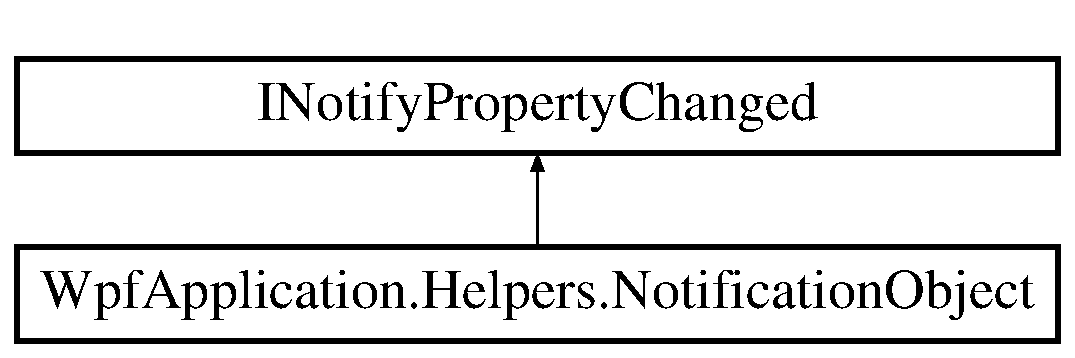
\includegraphics[height=2.000000cm]{class_wpf_application_1_1_helpers_1_1_notification_object}
\end{center}
\end{figure}
\subsection*{Protected Member Functions}
\begin{DoxyCompactItemize}
\item 
void \hyperlink{class_wpf_application_1_1_helpers_1_1_notification_object_ab671378a81112fc5a7270f83154c5ca9}{Raise\-Property\-Changed$<$ T $>$} (Expression$<$ Func$<$ T $>$$>$ action)
\end{DoxyCompactItemize}
\subsection*{Events}
\begin{DoxyCompactItemize}
\item 
Property\-Changed\-Event\-Handler \hyperlink{class_wpf_application_1_1_helpers_1_1_notification_object_a8cc654b2aceffe0471fea574dcd365e1}{Property\-Changed}
\end{DoxyCompactItemize}


\subsection{Member Function Documentation}
\hypertarget{class_wpf_application_1_1_helpers_1_1_notification_object_ab671378a81112fc5a7270f83154c5ca9}{\index{Wpf\-Application\-::\-Helpers\-::\-Notification\-Object@{Wpf\-Application\-::\-Helpers\-::\-Notification\-Object}!Raise\-Property\-Changed$<$ T $>$@{Raise\-Property\-Changed$<$ T $>$}}
\index{Raise\-Property\-Changed$<$ T $>$@{Raise\-Property\-Changed$<$ T $>$}!WpfApplication::Helpers::NotificationObject@{Wpf\-Application\-::\-Helpers\-::\-Notification\-Object}}
\subsubsection[{Raise\-Property\-Changed$<$ T $>$}]{\setlength{\rightskip}{0pt plus 5cm}void Wpf\-Application.\-Helpers.\-Notification\-Object.\-Raise\-Property\-Changed$<$ T $>$ (
\begin{DoxyParamCaption}
\item[{Expression$<$ Func$<$ T $>$$>$}]{action}
\end{DoxyParamCaption}
)\hspace{0.3cm}{\ttfamily [protected]}}}\label{class_wpf_application_1_1_helpers_1_1_notification_object_ab671378a81112fc5a7270f83154c5ca9}


\subsection{Event Documentation}
\hypertarget{class_wpf_application_1_1_helpers_1_1_notification_object_a8cc654b2aceffe0471fea574dcd365e1}{\index{Wpf\-Application\-::\-Helpers\-::\-Notification\-Object@{Wpf\-Application\-::\-Helpers\-::\-Notification\-Object}!Property\-Changed@{Property\-Changed}}
\index{Property\-Changed@{Property\-Changed}!WpfApplication::Helpers::NotificationObject@{Wpf\-Application\-::\-Helpers\-::\-Notification\-Object}}
\subsubsection[{Property\-Changed}]{\setlength{\rightskip}{0pt plus 5cm}Property\-Changed\-Event\-Handler Wpf\-Application.\-Helpers.\-Notification\-Object.\-Property\-Changed}}\label{class_wpf_application_1_1_helpers_1_1_notification_object_a8cc654b2aceffe0471fea574dcd365e1}


The documentation for this class was generated from the following file\-:\begin{DoxyCompactItemize}
\item 
C\-:/\-Users/dju/\-Documents/\-Visual Studio 2012/\-Projects/\-P\-P\-E/\-P\-P\-E3/\-Wpf\-Application/\-Helpers/\hyperlink{_notification_object_8cs}{Notification\-Object.\-cs}\end{DoxyCompactItemize}

\hypertarget{class_model_1_1_o_f_f_r_e1}{\section{Model.\-O\-F\-F\-R\-E1 Class Reference}
\label{class_model_1_1_o_f_f_r_e1}\index{Model.\-O\-F\-F\-R\-E1@{Model.\-O\-F\-F\-R\-E1}}
}


Aucune documentation sur les métadonnées n'est disponible.  


Inheritance diagram for Model.\-O\-F\-F\-R\-E1\-:\begin{figure}[H]
\begin{center}
\leavevmode
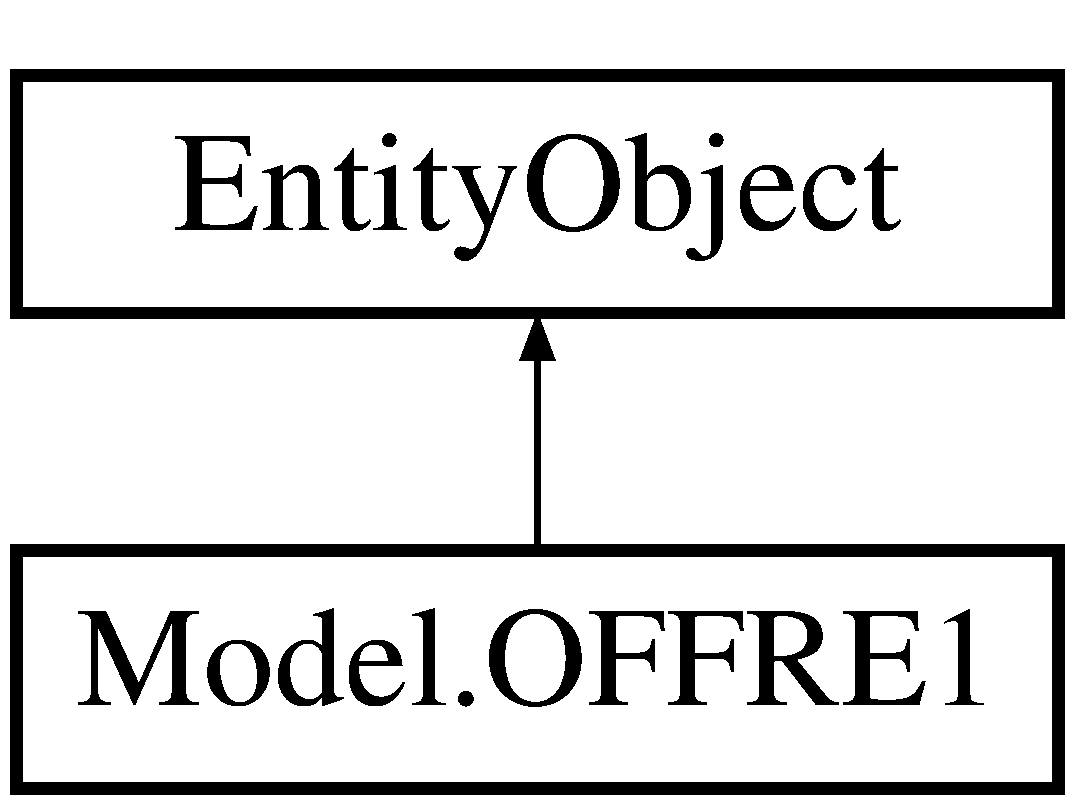
\includegraphics[height=2.000000cm]{class_model_1_1_o_f_f_r_e1}
\end{center}
\end{figure}
\subsection*{Static Public Member Functions}
\begin{DoxyCompactItemize}
\item 
static \hyperlink{class_model_1_1_o_f_f_r_e1}{O\-F\-F\-R\-E1} \hyperlink{class_model_1_1_o_f_f_r_e1_abb497ef2ec37783628503914a0b03e36}{Create\-O\-F\-F\-R\-E1} (global\-::\-System.\-Int32 \hyperlink{class_model_1_1_o_f_f_r_e1_ad57c3bdb1734c2de219aaf5267da7a33}{num\-\_\-rapport\-\_\-offre}, global\-::\-System.\-String \hyperlink{class_model_1_1_o_f_f_r_e1_abd3803160cf8cdb50d1d357bf379d82b}{depot\-\_\-legal\-\_\-offre})
\begin{DoxyCompactList}\small\item\em Créez un nouvel objet \hyperlink{class_model_1_1_o_f_f_r_e1}{O\-F\-F\-R\-E1}. \end{DoxyCompactList}\end{DoxyCompactItemize}
\subsection*{Properties}
\begin{DoxyCompactItemize}
\item 
Nullable$<$ global\-::\-System.\-Int32 $>$ \hyperlink{class_model_1_1_o_f_f_r_e1_a87716ad990cd87804edfa1ae5eecd1f7}{quantite\-\_\-offre}\hspace{0.3cm}{\ttfamily  \mbox{[}get, set\mbox{]}}
\begin{DoxyCompactList}\small\item\em Aucune documentation sur les métadonnées n'est disponible. \end{DoxyCompactList}\item 
global\-::\-System.\-Int32 \hyperlink{class_model_1_1_o_f_f_r_e1_ad57c3bdb1734c2de219aaf5267da7a33}{num\-\_\-rapport\-\_\-offre}\hspace{0.3cm}{\ttfamily  \mbox{[}get, set\mbox{]}}
\begin{DoxyCompactList}\small\item\em Aucune documentation sur les métadonnées n'est disponible. \end{DoxyCompactList}\item 
global\-::\-System.\-String \hyperlink{class_model_1_1_o_f_f_r_e1_abd3803160cf8cdb50d1d357bf379d82b}{depot\-\_\-legal\-\_\-offre}\hspace{0.3cm}{\ttfamily  \mbox{[}get, set\mbox{]}}
\begin{DoxyCompactList}\small\item\em Aucune documentation sur les métadonnées n'est disponible. \end{DoxyCompactList}\item 
\hyperlink{class_model_1_1_m_e_d_i_c_a_m_e_n_t}{M\-E\-D\-I\-C\-A\-M\-E\-N\-T} \hyperlink{class_model_1_1_o_f_f_r_e1_a2c69f629593dcb56e64724980441dfe6}{M\-E\-D\-I\-C\-A\-M\-E\-N\-T}\hspace{0.3cm}{\ttfamily  \mbox{[}get, set\mbox{]}}
\begin{DoxyCompactList}\small\item\em Aucune documentation sur les métadonnées n'est disponible. \end{DoxyCompactList}\item 
Entity\-Reference$<$ \hyperlink{class_model_1_1_m_e_d_i_c_a_m_e_n_t}{M\-E\-D\-I\-C\-A\-M\-E\-N\-T} $>$ \hyperlink{class_model_1_1_o_f_f_r_e1_a7725364d8165f3e4da799655ca3650a0}{M\-E\-D\-I\-C\-A\-M\-E\-N\-T\-Reference}\hspace{0.3cm}{\ttfamily  \mbox{[}get, set\mbox{]}}
\begin{DoxyCompactList}\small\item\em Aucune documentation sur les métadonnées n'est disponible. \end{DoxyCompactList}\item 
\hyperlink{class_model_1_1_r_a_p_p_o_r_t___d_e___v_i_s_i_t_e}{R\-A\-P\-P\-O\-R\-T\-\_\-\-D\-E\-\_\-\-V\-I\-S\-I\-T\-E} \hyperlink{class_model_1_1_o_f_f_r_e1_a87de6d87e3506d3826f5585b401137a0}{R\-A\-P\-P\-O\-R\-T\-\_\-\-D\-E\-\_\-\-V\-I\-S\-I\-T\-E}\hspace{0.3cm}{\ttfamily  \mbox{[}get, set\mbox{]}}
\begin{DoxyCompactList}\small\item\em Aucune documentation sur les métadonnées n'est disponible. \end{DoxyCompactList}\item 
Entity\-Reference\\*
$<$ \hyperlink{class_model_1_1_r_a_p_p_o_r_t___d_e___v_i_s_i_t_e}{R\-A\-P\-P\-O\-R\-T\-\_\-\-D\-E\-\_\-\-V\-I\-S\-I\-T\-E} $>$ \hyperlink{class_model_1_1_o_f_f_r_e1_a8234673a832a8f053a56a13434e9f664}{R\-A\-P\-P\-O\-R\-T\-\_\-\-D\-E\-\_\-\-V\-I\-S\-I\-T\-E\-Reference}\hspace{0.3cm}{\ttfamily  \mbox{[}get, set\mbox{]}}
\begin{DoxyCompactList}\small\item\em Aucune documentation sur les métadonnées n'est disponible. \end{DoxyCompactList}\end{DoxyCompactItemize}


\subsection{Detailed Description}
Aucune documentation sur les métadonnées n'est disponible. 



\subsection{Member Function Documentation}
\hypertarget{class_model_1_1_o_f_f_r_e1_abb497ef2ec37783628503914a0b03e36}{\index{Model\-::\-O\-F\-F\-R\-E1@{Model\-::\-O\-F\-F\-R\-E1}!Create\-O\-F\-F\-R\-E1@{Create\-O\-F\-F\-R\-E1}}
\index{Create\-O\-F\-F\-R\-E1@{Create\-O\-F\-F\-R\-E1}!Model::OFFRE1@{Model\-::\-O\-F\-F\-R\-E1}}
\subsubsection[{Create\-O\-F\-F\-R\-E1}]{\setlength{\rightskip}{0pt plus 5cm}static {\bf O\-F\-F\-R\-E1} Model.\-O\-F\-F\-R\-E1.\-Create\-O\-F\-F\-R\-E1 (
\begin{DoxyParamCaption}
\item[{global\-::\-System.\-Int32}]{num\-\_\-rapport\-\_\-offre, }
\item[{global\-::\-System.\-String}]{depot\-\_\-legal\-\_\-offre}
\end{DoxyParamCaption}
)\hspace{0.3cm}{\ttfamily [static]}}}\label{class_model_1_1_o_f_f_r_e1_abb497ef2ec37783628503914a0b03e36}


Créez un nouvel objet \hyperlink{class_model_1_1_o_f_f_r_e1}{O\-F\-F\-R\-E1}. 


\begin{DoxyParams}{Parameters}
{\em num\-\_\-rapport\-\_\-offre} & Valeur initiale de la propriété num\-\_\-rapport\-\_\-offre.\\
\hline
{\em depot\-\_\-legal\-\_\-offre} & Valeur initiale de la propriété depot\-\_\-legal\-\_\-offre.\\
\hline
\end{DoxyParams}


\subsection{Property Documentation}
\hypertarget{class_model_1_1_o_f_f_r_e1_abd3803160cf8cdb50d1d357bf379d82b}{\index{Model\-::\-O\-F\-F\-R\-E1@{Model\-::\-O\-F\-F\-R\-E1}!depot\-\_\-legal\-\_\-offre@{depot\-\_\-legal\-\_\-offre}}
\index{depot\-\_\-legal\-\_\-offre@{depot\-\_\-legal\-\_\-offre}!Model::OFFRE1@{Model\-::\-O\-F\-F\-R\-E1}}
\subsubsection[{depot\-\_\-legal\-\_\-offre}]{\setlength{\rightskip}{0pt plus 5cm}global.\-System.\-String Model.\-O\-F\-F\-R\-E1.\-depot\-\_\-legal\-\_\-offre\hspace{0.3cm}{\ttfamily [get]}, {\ttfamily [set]}}}\label{class_model_1_1_o_f_f_r_e1_abd3803160cf8cdb50d1d357bf379d82b}


Aucune documentation sur les métadonnées n'est disponible. 

\hypertarget{class_model_1_1_o_f_f_r_e1_a2c69f629593dcb56e64724980441dfe6}{\index{Model\-::\-O\-F\-F\-R\-E1@{Model\-::\-O\-F\-F\-R\-E1}!M\-E\-D\-I\-C\-A\-M\-E\-N\-T@{M\-E\-D\-I\-C\-A\-M\-E\-N\-T}}
\index{M\-E\-D\-I\-C\-A\-M\-E\-N\-T@{M\-E\-D\-I\-C\-A\-M\-E\-N\-T}!Model::OFFRE1@{Model\-::\-O\-F\-F\-R\-E1}}
\subsubsection[{M\-E\-D\-I\-C\-A\-M\-E\-N\-T}]{\setlength{\rightskip}{0pt plus 5cm}{\bf M\-E\-D\-I\-C\-A\-M\-E\-N\-T} Model.\-O\-F\-F\-R\-E1.\-M\-E\-D\-I\-C\-A\-M\-E\-N\-T\hspace{0.3cm}{\ttfamily [get]}, {\ttfamily [set]}}}\label{class_model_1_1_o_f_f_r_e1_a2c69f629593dcb56e64724980441dfe6}


Aucune documentation sur les métadonnées n'est disponible. 

\hypertarget{class_model_1_1_o_f_f_r_e1_a7725364d8165f3e4da799655ca3650a0}{\index{Model\-::\-O\-F\-F\-R\-E1@{Model\-::\-O\-F\-F\-R\-E1}!M\-E\-D\-I\-C\-A\-M\-E\-N\-T\-Reference@{M\-E\-D\-I\-C\-A\-M\-E\-N\-T\-Reference}}
\index{M\-E\-D\-I\-C\-A\-M\-E\-N\-T\-Reference@{M\-E\-D\-I\-C\-A\-M\-E\-N\-T\-Reference}!Model::OFFRE1@{Model\-::\-O\-F\-F\-R\-E1}}
\subsubsection[{M\-E\-D\-I\-C\-A\-M\-E\-N\-T\-Reference}]{\setlength{\rightskip}{0pt plus 5cm}Entity\-Reference$<${\bf M\-E\-D\-I\-C\-A\-M\-E\-N\-T}$>$ Model.\-O\-F\-F\-R\-E1.\-M\-E\-D\-I\-C\-A\-M\-E\-N\-T\-Reference\hspace{0.3cm}{\ttfamily [get]}, {\ttfamily [set]}}}\label{class_model_1_1_o_f_f_r_e1_a7725364d8165f3e4da799655ca3650a0}


Aucune documentation sur les métadonnées n'est disponible. 

\hypertarget{class_model_1_1_o_f_f_r_e1_ad57c3bdb1734c2de219aaf5267da7a33}{\index{Model\-::\-O\-F\-F\-R\-E1@{Model\-::\-O\-F\-F\-R\-E1}!num\-\_\-rapport\-\_\-offre@{num\-\_\-rapport\-\_\-offre}}
\index{num\-\_\-rapport\-\_\-offre@{num\-\_\-rapport\-\_\-offre}!Model::OFFRE1@{Model\-::\-O\-F\-F\-R\-E1}}
\subsubsection[{num\-\_\-rapport\-\_\-offre}]{\setlength{\rightskip}{0pt plus 5cm}global.\-System.\-Int32 Model.\-O\-F\-F\-R\-E1.\-num\-\_\-rapport\-\_\-offre\hspace{0.3cm}{\ttfamily [get]}, {\ttfamily [set]}}}\label{class_model_1_1_o_f_f_r_e1_ad57c3bdb1734c2de219aaf5267da7a33}


Aucune documentation sur les métadonnées n'est disponible. 

\hypertarget{class_model_1_1_o_f_f_r_e1_a87716ad990cd87804edfa1ae5eecd1f7}{\index{Model\-::\-O\-F\-F\-R\-E1@{Model\-::\-O\-F\-F\-R\-E1}!quantite\-\_\-offre@{quantite\-\_\-offre}}
\index{quantite\-\_\-offre@{quantite\-\_\-offre}!Model::OFFRE1@{Model\-::\-O\-F\-F\-R\-E1}}
\subsubsection[{quantite\-\_\-offre}]{\setlength{\rightskip}{0pt plus 5cm}Nullable$<$global.\-System.\-Int32$>$ Model.\-O\-F\-F\-R\-E1.\-quantite\-\_\-offre\hspace{0.3cm}{\ttfamily [get]}, {\ttfamily [set]}}}\label{class_model_1_1_o_f_f_r_e1_a87716ad990cd87804edfa1ae5eecd1f7}


Aucune documentation sur les métadonnées n'est disponible. 

\hypertarget{class_model_1_1_o_f_f_r_e1_a87de6d87e3506d3826f5585b401137a0}{\index{Model\-::\-O\-F\-F\-R\-E1@{Model\-::\-O\-F\-F\-R\-E1}!R\-A\-P\-P\-O\-R\-T\-\_\-\-D\-E\-\_\-\-V\-I\-S\-I\-T\-E@{R\-A\-P\-P\-O\-R\-T\-\_\-\-D\-E\-\_\-\-V\-I\-S\-I\-T\-E}}
\index{R\-A\-P\-P\-O\-R\-T\-\_\-\-D\-E\-\_\-\-V\-I\-S\-I\-T\-E@{R\-A\-P\-P\-O\-R\-T\-\_\-\-D\-E\-\_\-\-V\-I\-S\-I\-T\-E}!Model::OFFRE1@{Model\-::\-O\-F\-F\-R\-E1}}
\subsubsection[{R\-A\-P\-P\-O\-R\-T\-\_\-\-D\-E\-\_\-\-V\-I\-S\-I\-T\-E}]{\setlength{\rightskip}{0pt plus 5cm}{\bf R\-A\-P\-P\-O\-R\-T\-\_\-\-D\-E\-\_\-\-V\-I\-S\-I\-T\-E} Model.\-O\-F\-F\-R\-E1.\-R\-A\-P\-P\-O\-R\-T\-\_\-\-D\-E\-\_\-\-V\-I\-S\-I\-T\-E\hspace{0.3cm}{\ttfamily [get]}, {\ttfamily [set]}}}\label{class_model_1_1_o_f_f_r_e1_a87de6d87e3506d3826f5585b401137a0}


Aucune documentation sur les métadonnées n'est disponible. 

\hypertarget{class_model_1_1_o_f_f_r_e1_a8234673a832a8f053a56a13434e9f664}{\index{Model\-::\-O\-F\-F\-R\-E1@{Model\-::\-O\-F\-F\-R\-E1}!R\-A\-P\-P\-O\-R\-T\-\_\-\-D\-E\-\_\-\-V\-I\-S\-I\-T\-E\-Reference@{R\-A\-P\-P\-O\-R\-T\-\_\-\-D\-E\-\_\-\-V\-I\-S\-I\-T\-E\-Reference}}
\index{R\-A\-P\-P\-O\-R\-T\-\_\-\-D\-E\-\_\-\-V\-I\-S\-I\-T\-E\-Reference@{R\-A\-P\-P\-O\-R\-T\-\_\-\-D\-E\-\_\-\-V\-I\-S\-I\-T\-E\-Reference}!Model::OFFRE1@{Model\-::\-O\-F\-F\-R\-E1}}
\subsubsection[{R\-A\-P\-P\-O\-R\-T\-\_\-\-D\-E\-\_\-\-V\-I\-S\-I\-T\-E\-Reference}]{\setlength{\rightskip}{0pt plus 5cm}Entity\-Reference$<${\bf R\-A\-P\-P\-O\-R\-T\-\_\-\-D\-E\-\_\-\-V\-I\-S\-I\-T\-E}$>$ Model.\-O\-F\-F\-R\-E1.\-R\-A\-P\-P\-O\-R\-T\-\_\-\-D\-E\-\_\-\-V\-I\-S\-I\-T\-E\-Reference\hspace{0.3cm}{\ttfamily [get]}, {\ttfamily [set]}}}\label{class_model_1_1_o_f_f_r_e1_a8234673a832a8f053a56a13434e9f664}


Aucune documentation sur les métadonnées n'est disponible. 



The documentation for this class was generated from the following file\-:\begin{DoxyCompactItemize}
\item 
C\-:/\-Users/dju/\-Documents/\-Visual Studio 2012/\-Projects/\-P\-P\-E/\-P\-P\-E3/\-Model/\hyperlink{_model_bdd_sio_8_designer_8cs}{Model\-Bdd\-Sio.\-Designer.\-cs}\end{DoxyCompactItemize}

\hypertarget{class_wpf_application_1_1_view_model_1_1_password_encoder}{\section{Wpf\-Application.\-View\-Model.\-Password\-Encoder Class Reference}
\label{class_wpf_application_1_1_view_model_1_1_password_encoder}\index{Wpf\-Application.\-View\-Model.\-Password\-Encoder@{Wpf\-Application.\-View\-Model.\-Password\-Encoder}}
}
\subsection*{Public Member Functions}
\begin{DoxyCompactItemize}
\item 
string \hyperlink{class_wpf_application_1_1_view_model_1_1_password_encoder_ab3dc9bbeebf03ddfba650af3a771cdda}{encode\-Password} (string raw, string salt)
\end{DoxyCompactItemize}


\subsection{Member Function Documentation}
\hypertarget{class_wpf_application_1_1_view_model_1_1_password_encoder_ab3dc9bbeebf03ddfba650af3a771cdda}{\index{Wpf\-Application\-::\-View\-Model\-::\-Password\-Encoder@{Wpf\-Application\-::\-View\-Model\-::\-Password\-Encoder}!encode\-Password@{encode\-Password}}
\index{encode\-Password@{encode\-Password}!WpfApplication::ViewModel::PasswordEncoder@{Wpf\-Application\-::\-View\-Model\-::\-Password\-Encoder}}
\subsubsection[{encode\-Password}]{\setlength{\rightskip}{0pt plus 5cm}string Wpf\-Application.\-View\-Model.\-Password\-Encoder.\-encode\-Password (
\begin{DoxyParamCaption}
\item[{string}]{raw, }
\item[{string}]{salt}
\end{DoxyParamCaption}
)}}\label{class_wpf_application_1_1_view_model_1_1_password_encoder_ab3dc9bbeebf03ddfba650af3a771cdda}


The documentation for this class was generated from the following file\-:\begin{DoxyCompactItemize}
\item 
C\-:/\-Users/dju/\-Documents/\-Visual Studio 2012/\-Projects/\-P\-P\-E/\-P\-P\-E3/\-Wpf\-Application/\-View\-Model/\hyperlink{_password_encoder_8cs}{Password\-Encoder.\-cs}\end{DoxyCompactItemize}

\hypertarget{class_model_1_1helpers_1_1_pra_helper}{\section{Model.\-helpers.\-Pra\-Helper Class Reference}
\label{class_model_1_1helpers_1_1_pra_helper}\index{Model.\-helpers.\-Pra\-Helper@{Model.\-helpers.\-Pra\-Helper}}
}
\subsection*{Public Member Functions}
\begin{DoxyCompactItemize}
\item 
\hyperlink{class_model_1_1helpers_1_1_pra_helper_a8c9cd7c816ccb26ad9c3c82d0843e99c}{Pra\-Helper} ()
\item 
List$<$ \hyperlink{class_model_1_1_p_r_a_t_i_c_i_e_n}{P\-R\-A\-T\-I\-C\-I\-E\-N} $>$ \hyperlink{class_model_1_1helpers_1_1_pra_helper_a57cc7cb47128c4170db9a942da04d84e}{Get\-List} ()
\item 
void \hyperlink{class_model_1_1helpers_1_1_pra_helper_abb536bc7ef8a3661ed9148f7e4bec3b9}{Insert} (\hyperlink{class_model_1_1_p_r_a_t_i_c_i_e_n}{P\-R\-A\-T\-I\-C\-I\-E\-N} praticien)
\item 
void \hyperlink{class_model_1_1helpers_1_1_pra_helper_a9c43e8aff193128dc80135fad232c8bd}{Update} (\hyperlink{class_model_1_1_p_r_a_t_i_c_i_e_n}{P\-R\-A\-T\-I\-C\-I\-E\-N} praticien)
\item 
void \hyperlink{class_model_1_1helpers_1_1_pra_helper_a12c4b5afc31f107e2c915fd503733106}{Delete} (\hyperlink{class_model_1_1_p_r_a_t_i_c_i_e_n}{P\-R\-A\-T\-I\-C\-I\-E\-N} praticien)
\item 
\hyperlink{class_model_1_1_p_r_a_t_i_c_i_e_n}{P\-R\-A\-T\-I\-C\-I\-E\-N} \hyperlink{class_model_1_1helpers_1_1_pra_helper_a8c3228c86ce8e9b1206dceb1323be34d}{get\-By\-Id} (int id)
\end{DoxyCompactItemize}
\subsection*{Properties}
\begin{DoxyCompactItemize}
\item 
static \hyperlink{class_model_1_1helpers_1_1_pra_helper}{Pra\-Helper} \hyperlink{class_model_1_1helpers_1_1_pra_helper_a9fa42a78879906ceb14876fff51c9124}{Current}\hspace{0.3cm}{\ttfamily  \mbox{[}get\mbox{]}}
\begin{DoxyCompactList}\small\item\em This is a thread-\/safe, lazy singleton. See \href{http://www.yoda.arachsys.com/csharp/singleton.html}{\tt http\-://www.\-yoda.\-arachsys.\-com/csharp/singleton.\-html} for more details about its implementation. \end{DoxyCompactList}\end{DoxyCompactItemize}


\subsection{Constructor \& Destructor Documentation}
\hypertarget{class_model_1_1helpers_1_1_pra_helper_a8c9cd7c816ccb26ad9c3c82d0843e99c}{\index{Model\-::helpers\-::\-Pra\-Helper@{Model\-::helpers\-::\-Pra\-Helper}!Pra\-Helper@{Pra\-Helper}}
\index{Pra\-Helper@{Pra\-Helper}!Model::helpers::PraHelper@{Model\-::helpers\-::\-Pra\-Helper}}
\subsubsection[{Pra\-Helper}]{\setlength{\rightskip}{0pt plus 5cm}Model.\-helpers.\-Pra\-Helper.\-Pra\-Helper (
\begin{DoxyParamCaption}
{}
\end{DoxyParamCaption}
)}}\label{class_model_1_1helpers_1_1_pra_helper_a8c9cd7c816ccb26ad9c3c82d0843e99c}


\subsection{Member Function Documentation}
\hypertarget{class_model_1_1helpers_1_1_pra_helper_a12c4b5afc31f107e2c915fd503733106}{\index{Model\-::helpers\-::\-Pra\-Helper@{Model\-::helpers\-::\-Pra\-Helper}!Delete@{Delete}}
\index{Delete@{Delete}!Model::helpers::PraHelper@{Model\-::helpers\-::\-Pra\-Helper}}
\subsubsection[{Delete}]{\setlength{\rightskip}{0pt plus 5cm}void Model.\-helpers.\-Pra\-Helper.\-Delete (
\begin{DoxyParamCaption}
\item[{{\bf P\-R\-A\-T\-I\-C\-I\-E\-N}}]{praticien}
\end{DoxyParamCaption}
)}}\label{class_model_1_1helpers_1_1_pra_helper_a12c4b5afc31f107e2c915fd503733106}
\hypertarget{class_model_1_1helpers_1_1_pra_helper_a8c3228c86ce8e9b1206dceb1323be34d}{\index{Model\-::helpers\-::\-Pra\-Helper@{Model\-::helpers\-::\-Pra\-Helper}!get\-By\-Id@{get\-By\-Id}}
\index{get\-By\-Id@{get\-By\-Id}!Model::helpers::PraHelper@{Model\-::helpers\-::\-Pra\-Helper}}
\subsubsection[{get\-By\-Id}]{\setlength{\rightskip}{0pt plus 5cm}{\bf P\-R\-A\-T\-I\-C\-I\-E\-N} Model.\-helpers.\-Pra\-Helper.\-get\-By\-Id (
\begin{DoxyParamCaption}
\item[{int}]{id}
\end{DoxyParamCaption}
)}}\label{class_model_1_1helpers_1_1_pra_helper_a8c3228c86ce8e9b1206dceb1323be34d}
\hypertarget{class_model_1_1helpers_1_1_pra_helper_a57cc7cb47128c4170db9a942da04d84e}{\index{Model\-::helpers\-::\-Pra\-Helper@{Model\-::helpers\-::\-Pra\-Helper}!Get\-List@{Get\-List}}
\index{Get\-List@{Get\-List}!Model::helpers::PraHelper@{Model\-::helpers\-::\-Pra\-Helper}}
\subsubsection[{Get\-List}]{\setlength{\rightskip}{0pt plus 5cm}List$<${\bf P\-R\-A\-T\-I\-C\-I\-E\-N}$>$ Model.\-helpers.\-Pra\-Helper.\-Get\-List (
\begin{DoxyParamCaption}
{}
\end{DoxyParamCaption}
)}}\label{class_model_1_1helpers_1_1_pra_helper_a57cc7cb47128c4170db9a942da04d84e}
\hypertarget{class_model_1_1helpers_1_1_pra_helper_abb536bc7ef8a3661ed9148f7e4bec3b9}{\index{Model\-::helpers\-::\-Pra\-Helper@{Model\-::helpers\-::\-Pra\-Helper}!Insert@{Insert}}
\index{Insert@{Insert}!Model::helpers::PraHelper@{Model\-::helpers\-::\-Pra\-Helper}}
\subsubsection[{Insert}]{\setlength{\rightskip}{0pt plus 5cm}void Model.\-helpers.\-Pra\-Helper.\-Insert (
\begin{DoxyParamCaption}
\item[{{\bf P\-R\-A\-T\-I\-C\-I\-E\-N}}]{praticien}
\end{DoxyParamCaption}
)}}\label{class_model_1_1helpers_1_1_pra_helper_abb536bc7ef8a3661ed9148f7e4bec3b9}
\hypertarget{class_model_1_1helpers_1_1_pra_helper_a9c43e8aff193128dc80135fad232c8bd}{\index{Model\-::helpers\-::\-Pra\-Helper@{Model\-::helpers\-::\-Pra\-Helper}!Update@{Update}}
\index{Update@{Update}!Model::helpers::PraHelper@{Model\-::helpers\-::\-Pra\-Helper}}
\subsubsection[{Update}]{\setlength{\rightskip}{0pt plus 5cm}void Model.\-helpers.\-Pra\-Helper.\-Update (
\begin{DoxyParamCaption}
\item[{{\bf P\-R\-A\-T\-I\-C\-I\-E\-N}}]{praticien}
\end{DoxyParamCaption}
)}}\label{class_model_1_1helpers_1_1_pra_helper_a9c43e8aff193128dc80135fad232c8bd}


\subsection{Property Documentation}
\hypertarget{class_model_1_1helpers_1_1_pra_helper_a9fa42a78879906ceb14876fff51c9124}{\index{Model\-::helpers\-::\-Pra\-Helper@{Model\-::helpers\-::\-Pra\-Helper}!Current@{Current}}
\index{Current@{Current}!Model::helpers::PraHelper@{Model\-::helpers\-::\-Pra\-Helper}}
\subsubsection[{Current}]{\setlength{\rightskip}{0pt plus 5cm}{\bf Pra\-Helper} Model.\-helpers.\-Pra\-Helper.\-Current\hspace{0.3cm}{\ttfamily [static]}, {\ttfamily [get]}}}\label{class_model_1_1helpers_1_1_pra_helper_a9fa42a78879906ceb14876fff51c9124}


This is a thread-\/safe, lazy singleton. See \href{http://www.yoda.arachsys.com/csharp/singleton.html}{\tt http\-://www.\-yoda.\-arachsys.\-com/csharp/singleton.\-html} for more details about its implementation. 



The documentation for this class was generated from the following file\-:\begin{DoxyCompactItemize}
\item 
C\-:/\-Users/dju/\-Documents/\-Visual Studio 2012/\-Projects/\-P\-P\-E/\-P\-P\-E3/\-Model/helpers/\hyperlink{_pra_helper_8cs}{Pra\-Helper.\-cs}\end{DoxyCompactItemize}

\hypertarget{class_model_1_1_p_r_a_t_i_c_i_e_n}{\section{Model.\-P\-R\-A\-T\-I\-C\-I\-E\-N Class Reference}
\label{class_model_1_1_p_r_a_t_i_c_i_e_n}\index{Model.\-P\-R\-A\-T\-I\-C\-I\-E\-N@{Model.\-P\-R\-A\-T\-I\-C\-I\-E\-N}}
}


Aucune documentation sur les métadonnées n'est disponible.  


Inheritance diagram for Model.\-P\-R\-A\-T\-I\-C\-I\-E\-N\-:\begin{figure}[H]
\begin{center}
\leavevmode
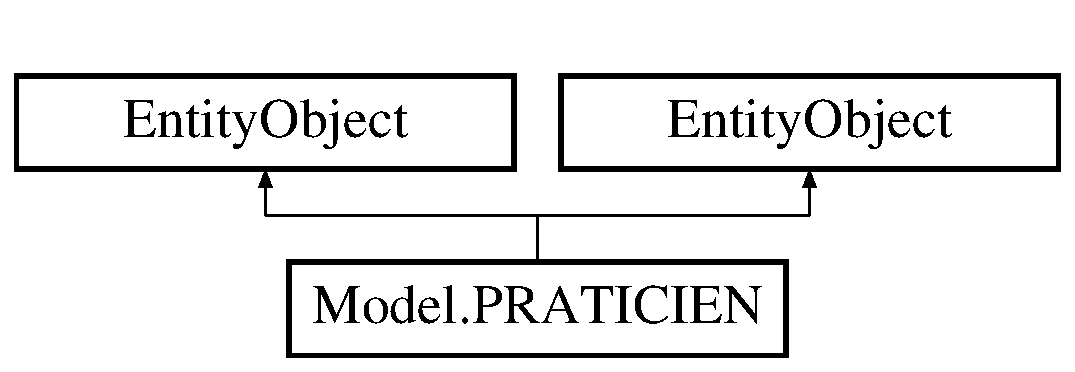
\includegraphics[height=2.000000cm]{class_model_1_1_p_r_a_t_i_c_i_e_n}
\end{center}
\end{figure}
\subsection*{Public Member Functions}
\begin{DoxyCompactItemize}
\item 
override string \hyperlink{class_model_1_1_p_r_a_t_i_c_i_e_n_ac980c0c57fc1a58f8681bd6590f099a2}{To\-String} ()
\end{DoxyCompactItemize}
\subsection*{Static Public Member Functions}
\begin{DoxyCompactItemize}
\item 
static \hyperlink{class_model_1_1_p_r_a_t_i_c_i_e_n}{P\-R\-A\-T\-I\-C\-I\-E\-N} \hyperlink{class_model_1_1_p_r_a_t_i_c_i_e_n_acd3d36c30b2afe182c8977a6307379ac}{Create\-P\-R\-A\-T\-I\-C\-I\-E\-N} (global\-::\-System.\-Int32 \hyperlink{class_model_1_1_p_r_a_t_i_c_i_e_n_abe4fab1270371ef15fc1342a8d048d26}{matricule\-\_\-praticien}, global\-::\-System.\-String \hyperlink{class_model_1_1_p_r_a_t_i_c_i_e_n_a2fa0f78d1573fe2d7d39d0a18feced05}{prenom\-\_\-praticien}, global\-::\-System.\-String \hyperlink{class_model_1_1_p_r_a_t_i_c_i_e_n_aebc5f079e73aca7fde020d817a1be78d}{nom\-\_\-praticien}, global\-::\-System.\-String \hyperlink{class_model_1_1_p_r_a_t_i_c_i_e_n_af65b1cb99d1ba84d1f1a3c9d4ff96637}{adresse\-\_\-praticien}, global\-::\-System.\-String \hyperlink{class_model_1_1_p_r_a_t_i_c_i_e_n_a2a75459147811d5a57c500054d647925}{cp\-\_\-praticien}, global\-::\-System.\-String \hyperlink{class_model_1_1_p_r_a_t_i_c_i_e_n_ae32f7c05fd2519a7a0b308ba1117856a}{ville\-\_\-praticien}, global\-::\-System.\-Double \hyperlink{class_model_1_1_p_r_a_t_i_c_i_e_n_af7a6f895c280db516f12fdf90e207bae}{coefnotoriete\-\_\-praticien}, global\-::\-System.\-Boolean \hyperlink{class_model_1_1_p_r_a_t_i_c_i_e_n_aab525a0862d5b0b441b850563c7f2a69}{titulaire\-\_\-praticien}, global\-::\-System.\-String \hyperlink{class_model_1_1_p_r_a_t_i_c_i_e_n_a3182fceec324d9beb52831dd2f36af6f}{num\-Tel})
\begin{DoxyCompactList}\small\item\em Créez un nouvel objet \hyperlink{class_model_1_1_p_r_a_t_i_c_i_e_n}{P\-R\-A\-T\-I\-C\-I\-E\-N}. \end{DoxyCompactList}\end{DoxyCompactItemize}
\subsection*{Properties}
\begin{DoxyCompactItemize}
\item 
global\-::\-System.\-Int32 \hyperlink{class_model_1_1_p_r_a_t_i_c_i_e_n_abe4fab1270371ef15fc1342a8d048d26}{matricule\-\_\-praticien}\hspace{0.3cm}{\ttfamily  \mbox{[}get, set\mbox{]}}
\begin{DoxyCompactList}\small\item\em Aucune documentation sur les métadonnées n'est disponible. \end{DoxyCompactList}\item 
Nullable$<$ global\-::\-System.\-Int32 $>$ \hyperlink{class_model_1_1_p_r_a_t_i_c_i_e_n_ab93a1451efbd3e55b088b40837f035b5}{code\-\_\-type}\hspace{0.3cm}{\ttfamily  \mbox{[}get, set\mbox{]}}
\begin{DoxyCompactList}\small\item\em Aucune documentation sur les métadonnées n'est disponible. \end{DoxyCompactList}\item 
global\-::\-System.\-String \hyperlink{class_model_1_1_p_r_a_t_i_c_i_e_n_a2fa0f78d1573fe2d7d39d0a18feced05}{prenom\-\_\-praticien}\hspace{0.3cm}{\ttfamily  \mbox{[}get, set\mbox{]}}
\begin{DoxyCompactList}\small\item\em Aucune documentation sur les métadonnées n'est disponible. \end{DoxyCompactList}\item 
global\-::\-System.\-String \hyperlink{class_model_1_1_p_r_a_t_i_c_i_e_n_aebc5f079e73aca7fde020d817a1be78d}{nom\-\_\-praticien}\hspace{0.3cm}{\ttfamily  \mbox{[}get, set\mbox{]}}
\begin{DoxyCompactList}\small\item\em Aucune documentation sur les métadonnées n'est disponible. \end{DoxyCompactList}\item 
global\-::\-System.\-String \hyperlink{class_model_1_1_p_r_a_t_i_c_i_e_n_af65b1cb99d1ba84d1f1a3c9d4ff96637}{adresse\-\_\-praticien}\hspace{0.3cm}{\ttfamily  \mbox{[}get, set\mbox{]}}
\begin{DoxyCompactList}\small\item\em Aucune documentation sur les métadonnées n'est disponible. \end{DoxyCompactList}\item 
global\-::\-System.\-String \hyperlink{class_model_1_1_p_r_a_t_i_c_i_e_n_a2a75459147811d5a57c500054d647925}{cp\-\_\-praticien}\hspace{0.3cm}{\ttfamily  \mbox{[}get, set\mbox{]}}
\begin{DoxyCompactList}\small\item\em Aucune documentation sur les métadonnées n'est disponible. \end{DoxyCompactList}\item 
global\-::\-System.\-String \hyperlink{class_model_1_1_p_r_a_t_i_c_i_e_n_ae32f7c05fd2519a7a0b308ba1117856a}{ville\-\_\-praticien}\hspace{0.3cm}{\ttfamily  \mbox{[}get, set\mbox{]}}
\begin{DoxyCompactList}\small\item\em Aucune documentation sur les métadonnées n'est disponible. \end{DoxyCompactList}\item 
global\-::\-System.\-Double \hyperlink{class_model_1_1_p_r_a_t_i_c_i_e_n_af7a6f895c280db516f12fdf90e207bae}{coefnotoriete\-\_\-praticien}\hspace{0.3cm}{\ttfamily  \mbox{[}get, set\mbox{]}}
\begin{DoxyCompactList}\small\item\em Aucune documentation sur les métadonnées n'est disponible. \end{DoxyCompactList}\item 
global\-::\-System.\-Boolean \hyperlink{class_model_1_1_p_r_a_t_i_c_i_e_n_aab525a0862d5b0b441b850563c7f2a69}{titulaire\-\_\-praticien}\hspace{0.3cm}{\ttfamily  \mbox{[}get, set\mbox{]}}
\begin{DoxyCompactList}\small\item\em Aucune documentation sur les métadonnées n'est disponible. \end{DoxyCompactList}\item 
global\-::\-System.\-String \hyperlink{class_model_1_1_p_r_a_t_i_c_i_e_n_a3182fceec324d9beb52831dd2f36af6f}{num\-Tel}\hspace{0.3cm}{\ttfamily  \mbox{[}get, set\mbox{]}}
\begin{DoxyCompactList}\small\item\em Aucune documentation sur les métadonnées n'est disponible. \end{DoxyCompactList}\item 
\hyperlink{class_model_1_1_t_y_p_e___p_r_a_t_i_c_i_e_n}{T\-Y\-P\-E\-\_\-\-P\-R\-A\-T\-I\-C\-I\-E\-N} \hyperlink{class_model_1_1_p_r_a_t_i_c_i_e_n_ab44028a89527b640b54ed235f767ecb0}{T\-Y\-P\-E\-\_\-\-P\-R\-A\-T\-I\-C\-I\-E\-N}\hspace{0.3cm}{\ttfamily  \mbox{[}get, set\mbox{]}}
\begin{DoxyCompactList}\small\item\em Aucune documentation sur les métadonnées n'est disponible. \end{DoxyCompactList}\item 
Entity\-Reference$<$ \hyperlink{class_model_1_1_t_y_p_e___p_r_a_t_i_c_i_e_n}{T\-Y\-P\-E\-\_\-\-P\-R\-A\-T\-I\-C\-I\-E\-N} $>$ \hyperlink{class_model_1_1_p_r_a_t_i_c_i_e_n_a3bc7693b4b3965bf78d0685094994c1e}{T\-Y\-P\-E\-\_\-\-P\-R\-A\-T\-I\-C\-I\-E\-N\-Reference}\hspace{0.3cm}{\ttfamily  \mbox{[}get, set\mbox{]}}
\begin{DoxyCompactList}\small\item\em Aucune documentation sur les métadonnées n'est disponible. \end{DoxyCompactList}\item 
Entity\-Collection\\*
$<$ \hyperlink{class_model_1_1_r_a_p_p_o_r_t___d_e___v_i_s_i_t_e}{R\-A\-P\-P\-O\-R\-T\-\_\-\-D\-E\-\_\-\-V\-I\-S\-I\-T\-E} $>$ \hyperlink{class_model_1_1_p_r_a_t_i_c_i_e_n_a75d092c7410cd4c92c2aee3d4cf884a6}{R\-A\-P\-P\-O\-R\-T\-\_\-\-D\-E\-\_\-\-V\-I\-S\-I\-T\-E}\hspace{0.3cm}{\ttfamily  \mbox{[}get, set\mbox{]}}
\begin{DoxyCompactList}\small\item\em Aucune documentation sur les métadonnées n'est disponible. \end{DoxyCompactList}\item 
Entity\-Collection$<$ \hyperlink{class_model_1_1_r_e_m_p_l_a_c_e}{R\-E\-M\-P\-L\-A\-C\-E} $>$ \hyperlink{class_model_1_1_p_r_a_t_i_c_i_e_n_a8ba2a460b9a92f0d33ebeb34a4fa6064}{R\-E\-M\-P\-L\-A\-C\-E}\hspace{0.3cm}{\ttfamily  \mbox{[}get, set\mbox{]}}
\begin{DoxyCompactList}\small\item\em Aucune documentation sur les métadonnées n'est disponible. \end{DoxyCompactList}\item 
Entity\-Collection$<$ \hyperlink{class_model_1_1_r_e_m_p_l_a_c_e}{R\-E\-M\-P\-L\-A\-C\-E} $>$ \hyperlink{class_model_1_1_p_r_a_t_i_c_i_e_n_a3f3d71a138657c92174f6452aa7e6a31}{R\-E\-M\-P\-L\-A\-C\-E1}\hspace{0.3cm}{\ttfamily  \mbox{[}get, set\mbox{]}}
\begin{DoxyCompactList}\small\item\em Aucune documentation sur les métadonnées n'est disponible. \end{DoxyCompactList}\item 
Entity\-Collection\\*
$<$ \hyperlink{class_model_1_1_a_c_t_i_v_i_t_e___c_o_m_p_l_e_m_e_n_t_a_i_r_e}{A\-C\-T\-I\-V\-I\-T\-E\-\_\-\-C\-O\-M\-P\-L\-E\-M\-E\-N\-T\-A\-I\-R\-E} $>$ \hyperlink{class_model_1_1_p_r_a_t_i_c_i_e_n_af38b58649915c0ec56ae505fe0bec260}{A\-C\-T\-I\-V\-I\-T\-E\-\_\-\-C\-O\-M\-P\-L\-E\-M\-E\-N\-T\-A\-I\-R\-E}\hspace{0.3cm}{\ttfamily  \mbox{[}get, set\mbox{]}}
\begin{DoxyCompactList}\small\item\em Aucune documentation sur les métadonnées n'est disponible. \end{DoxyCompactList}\item 
Entity\-Collection$<$ \hyperlink{class_model_1_1_s_p_e_c_i_a_l_i_t_e}{S\-P\-E\-C\-I\-A\-L\-I\-T\-E} $>$ \hyperlink{class_model_1_1_p_r_a_t_i_c_i_e_n_a15a32a4f8d3a3abc5d4644d2c9b5d29e}{S\-P\-E\-C\-I\-A\-L\-I\-T\-E}\hspace{0.3cm}{\ttfamily  \mbox{[}get, set\mbox{]}}
\begin{DoxyCompactList}\small\item\em Aucune documentation sur les métadonnées n'est disponible. \end{DoxyCompactList}\end{DoxyCompactItemize}


\subsection{Detailed Description}
Aucune documentation sur les métadonnées n'est disponible. 



\subsection{Member Function Documentation}
\hypertarget{class_model_1_1_p_r_a_t_i_c_i_e_n_acd3d36c30b2afe182c8977a6307379ac}{\index{Model\-::\-P\-R\-A\-T\-I\-C\-I\-E\-N@{Model\-::\-P\-R\-A\-T\-I\-C\-I\-E\-N}!Create\-P\-R\-A\-T\-I\-C\-I\-E\-N@{Create\-P\-R\-A\-T\-I\-C\-I\-E\-N}}
\index{Create\-P\-R\-A\-T\-I\-C\-I\-E\-N@{Create\-P\-R\-A\-T\-I\-C\-I\-E\-N}!Model::PRATICIEN@{Model\-::\-P\-R\-A\-T\-I\-C\-I\-E\-N}}
\subsubsection[{Create\-P\-R\-A\-T\-I\-C\-I\-E\-N}]{\setlength{\rightskip}{0pt plus 5cm}static {\bf P\-R\-A\-T\-I\-C\-I\-E\-N} Model.\-P\-R\-A\-T\-I\-C\-I\-E\-N.\-Create\-P\-R\-A\-T\-I\-C\-I\-E\-N (
\begin{DoxyParamCaption}
\item[{global\-::\-System.\-Int32}]{matricule\-\_\-praticien, }
\item[{global\-::\-System.\-String}]{prenom\-\_\-praticien, }
\item[{global\-::\-System.\-String}]{nom\-\_\-praticien, }
\item[{global\-::\-System.\-String}]{adresse\-\_\-praticien, }
\item[{global\-::\-System.\-String}]{cp\-\_\-praticien, }
\item[{global\-::\-System.\-String}]{ville\-\_\-praticien, }
\item[{global\-::\-System.\-Double}]{coefnotoriete\-\_\-praticien, }
\item[{global\-::\-System.\-Boolean}]{titulaire\-\_\-praticien, }
\item[{global\-::\-System.\-String}]{num\-Tel}
\end{DoxyParamCaption}
)\hspace{0.3cm}{\ttfamily [static]}}}\label{class_model_1_1_p_r_a_t_i_c_i_e_n_acd3d36c30b2afe182c8977a6307379ac}


Créez un nouvel objet \hyperlink{class_model_1_1_p_r_a_t_i_c_i_e_n}{P\-R\-A\-T\-I\-C\-I\-E\-N}. 


\begin{DoxyParams}{Parameters}
{\em matricule\-\_\-praticien} & Valeur initiale de la propriété matricule\-\_\-praticien.\\
\hline
{\em prenom\-\_\-praticien} & Valeur initiale de la propriété prenom\-\_\-praticien.\\
\hline
{\em nom\-\_\-praticien} & Valeur initiale de la propriété nom\-\_\-praticien.\\
\hline
{\em adresse\-\_\-praticien} & Valeur initiale de la propriété adresse\-\_\-praticien.\\
\hline
{\em cp\-\_\-praticien} & Valeur initiale de la propriété cp\-\_\-praticien.\\
\hline
{\em ville\-\_\-praticien} & Valeur initiale de la propriété ville\-\_\-praticien.\\
\hline
{\em coefnotoriete\-\_\-praticien} & Valeur initiale de la propriété coefnotoriete\-\_\-praticien.\\
\hline
{\em titulaire\-\_\-praticien} & Valeur initiale de la propriété titulaire\-\_\-praticien.\\
\hline
{\em num\-Tel} & Valeur initiale de la propriété num\-Tel.\\
\hline
\end{DoxyParams}
\hypertarget{class_model_1_1_p_r_a_t_i_c_i_e_n_ac980c0c57fc1a58f8681bd6590f099a2}{\index{Model\-::\-P\-R\-A\-T\-I\-C\-I\-E\-N@{Model\-::\-P\-R\-A\-T\-I\-C\-I\-E\-N}!To\-String@{To\-String}}
\index{To\-String@{To\-String}!Model::PRATICIEN@{Model\-::\-P\-R\-A\-T\-I\-C\-I\-E\-N}}
\subsubsection[{To\-String}]{\setlength{\rightskip}{0pt plus 5cm}override string Model.\-P\-R\-A\-T\-I\-C\-I\-E\-N.\-To\-String (
\begin{DoxyParamCaption}
{}
\end{DoxyParamCaption}
)}}\label{class_model_1_1_p_r_a_t_i_c_i_e_n_ac980c0c57fc1a58f8681bd6590f099a2}


\subsection{Property Documentation}
\hypertarget{class_model_1_1_p_r_a_t_i_c_i_e_n_af38b58649915c0ec56ae505fe0bec260}{\index{Model\-::\-P\-R\-A\-T\-I\-C\-I\-E\-N@{Model\-::\-P\-R\-A\-T\-I\-C\-I\-E\-N}!A\-C\-T\-I\-V\-I\-T\-E\-\_\-\-C\-O\-M\-P\-L\-E\-M\-E\-N\-T\-A\-I\-R\-E@{A\-C\-T\-I\-V\-I\-T\-E\-\_\-\-C\-O\-M\-P\-L\-E\-M\-E\-N\-T\-A\-I\-R\-E}}
\index{A\-C\-T\-I\-V\-I\-T\-E\-\_\-\-C\-O\-M\-P\-L\-E\-M\-E\-N\-T\-A\-I\-R\-E@{A\-C\-T\-I\-V\-I\-T\-E\-\_\-\-C\-O\-M\-P\-L\-E\-M\-E\-N\-T\-A\-I\-R\-E}!Model::PRATICIEN@{Model\-::\-P\-R\-A\-T\-I\-C\-I\-E\-N}}
\subsubsection[{A\-C\-T\-I\-V\-I\-T\-E\-\_\-\-C\-O\-M\-P\-L\-E\-M\-E\-N\-T\-A\-I\-R\-E}]{\setlength{\rightskip}{0pt plus 5cm}Entity\-Collection$<${\bf A\-C\-T\-I\-V\-I\-T\-E\-\_\-\-C\-O\-M\-P\-L\-E\-M\-E\-N\-T\-A\-I\-R\-E}$>$ Model.\-P\-R\-A\-T\-I\-C\-I\-E\-N.\-A\-C\-T\-I\-V\-I\-T\-E\-\_\-\-C\-O\-M\-P\-L\-E\-M\-E\-N\-T\-A\-I\-R\-E\hspace{0.3cm}{\ttfamily [get]}, {\ttfamily [set]}}}\label{class_model_1_1_p_r_a_t_i_c_i_e_n_af38b58649915c0ec56ae505fe0bec260}


Aucune documentation sur les métadonnées n'est disponible. 

\hypertarget{class_model_1_1_p_r_a_t_i_c_i_e_n_af65b1cb99d1ba84d1f1a3c9d4ff96637}{\index{Model\-::\-P\-R\-A\-T\-I\-C\-I\-E\-N@{Model\-::\-P\-R\-A\-T\-I\-C\-I\-E\-N}!adresse\-\_\-praticien@{adresse\-\_\-praticien}}
\index{adresse\-\_\-praticien@{adresse\-\_\-praticien}!Model::PRATICIEN@{Model\-::\-P\-R\-A\-T\-I\-C\-I\-E\-N}}
\subsubsection[{adresse\-\_\-praticien}]{\setlength{\rightskip}{0pt plus 5cm}global.\-System.\-String Model.\-P\-R\-A\-T\-I\-C\-I\-E\-N.\-adresse\-\_\-praticien\hspace{0.3cm}{\ttfamily [get]}, {\ttfamily [set]}}}\label{class_model_1_1_p_r_a_t_i_c_i_e_n_af65b1cb99d1ba84d1f1a3c9d4ff96637}


Aucune documentation sur les métadonnées n'est disponible. 

\hypertarget{class_model_1_1_p_r_a_t_i_c_i_e_n_ab93a1451efbd3e55b088b40837f035b5}{\index{Model\-::\-P\-R\-A\-T\-I\-C\-I\-E\-N@{Model\-::\-P\-R\-A\-T\-I\-C\-I\-E\-N}!code\-\_\-type@{code\-\_\-type}}
\index{code\-\_\-type@{code\-\_\-type}!Model::PRATICIEN@{Model\-::\-P\-R\-A\-T\-I\-C\-I\-E\-N}}
\subsubsection[{code\-\_\-type}]{\setlength{\rightskip}{0pt plus 5cm}Nullable$<$global.\-System.\-Int32$>$ Model.\-P\-R\-A\-T\-I\-C\-I\-E\-N.\-code\-\_\-type\hspace{0.3cm}{\ttfamily [get]}, {\ttfamily [set]}}}\label{class_model_1_1_p_r_a_t_i_c_i_e_n_ab93a1451efbd3e55b088b40837f035b5}


Aucune documentation sur les métadonnées n'est disponible. 

\hypertarget{class_model_1_1_p_r_a_t_i_c_i_e_n_af7a6f895c280db516f12fdf90e207bae}{\index{Model\-::\-P\-R\-A\-T\-I\-C\-I\-E\-N@{Model\-::\-P\-R\-A\-T\-I\-C\-I\-E\-N}!coefnotoriete\-\_\-praticien@{coefnotoriete\-\_\-praticien}}
\index{coefnotoriete\-\_\-praticien@{coefnotoriete\-\_\-praticien}!Model::PRATICIEN@{Model\-::\-P\-R\-A\-T\-I\-C\-I\-E\-N}}
\subsubsection[{coefnotoriete\-\_\-praticien}]{\setlength{\rightskip}{0pt plus 5cm}global.\-System.\-Double Model.\-P\-R\-A\-T\-I\-C\-I\-E\-N.\-coefnotoriete\-\_\-praticien\hspace{0.3cm}{\ttfamily [get]}, {\ttfamily [set]}}}\label{class_model_1_1_p_r_a_t_i_c_i_e_n_af7a6f895c280db516f12fdf90e207bae}


Aucune documentation sur les métadonnées n'est disponible. 

\hypertarget{class_model_1_1_p_r_a_t_i_c_i_e_n_a2a75459147811d5a57c500054d647925}{\index{Model\-::\-P\-R\-A\-T\-I\-C\-I\-E\-N@{Model\-::\-P\-R\-A\-T\-I\-C\-I\-E\-N}!cp\-\_\-praticien@{cp\-\_\-praticien}}
\index{cp\-\_\-praticien@{cp\-\_\-praticien}!Model::PRATICIEN@{Model\-::\-P\-R\-A\-T\-I\-C\-I\-E\-N}}
\subsubsection[{cp\-\_\-praticien}]{\setlength{\rightskip}{0pt plus 5cm}global.\-System.\-String Model.\-P\-R\-A\-T\-I\-C\-I\-E\-N.\-cp\-\_\-praticien\hspace{0.3cm}{\ttfamily [get]}, {\ttfamily [set]}}}\label{class_model_1_1_p_r_a_t_i_c_i_e_n_a2a75459147811d5a57c500054d647925}


Aucune documentation sur les métadonnées n'est disponible. 

\hypertarget{class_model_1_1_p_r_a_t_i_c_i_e_n_abe4fab1270371ef15fc1342a8d048d26}{\index{Model\-::\-P\-R\-A\-T\-I\-C\-I\-E\-N@{Model\-::\-P\-R\-A\-T\-I\-C\-I\-E\-N}!matricule\-\_\-praticien@{matricule\-\_\-praticien}}
\index{matricule\-\_\-praticien@{matricule\-\_\-praticien}!Model::PRATICIEN@{Model\-::\-P\-R\-A\-T\-I\-C\-I\-E\-N}}
\subsubsection[{matricule\-\_\-praticien}]{\setlength{\rightskip}{0pt plus 5cm}global.\-System.\-Int32 Model.\-P\-R\-A\-T\-I\-C\-I\-E\-N.\-matricule\-\_\-praticien\hspace{0.3cm}{\ttfamily [get]}, {\ttfamily [set]}}}\label{class_model_1_1_p_r_a_t_i_c_i_e_n_abe4fab1270371ef15fc1342a8d048d26}


Aucune documentation sur les métadonnées n'est disponible. 

\hypertarget{class_model_1_1_p_r_a_t_i_c_i_e_n_aebc5f079e73aca7fde020d817a1be78d}{\index{Model\-::\-P\-R\-A\-T\-I\-C\-I\-E\-N@{Model\-::\-P\-R\-A\-T\-I\-C\-I\-E\-N}!nom\-\_\-praticien@{nom\-\_\-praticien}}
\index{nom\-\_\-praticien@{nom\-\_\-praticien}!Model::PRATICIEN@{Model\-::\-P\-R\-A\-T\-I\-C\-I\-E\-N}}
\subsubsection[{nom\-\_\-praticien}]{\setlength{\rightskip}{0pt plus 5cm}global.\-System.\-String Model.\-P\-R\-A\-T\-I\-C\-I\-E\-N.\-nom\-\_\-praticien\hspace{0.3cm}{\ttfamily [get]}, {\ttfamily [set]}}}\label{class_model_1_1_p_r_a_t_i_c_i_e_n_aebc5f079e73aca7fde020d817a1be78d}


Aucune documentation sur les métadonnées n'est disponible. 

\hypertarget{class_model_1_1_p_r_a_t_i_c_i_e_n_a3182fceec324d9beb52831dd2f36af6f}{\index{Model\-::\-P\-R\-A\-T\-I\-C\-I\-E\-N@{Model\-::\-P\-R\-A\-T\-I\-C\-I\-E\-N}!num\-Tel@{num\-Tel}}
\index{num\-Tel@{num\-Tel}!Model::PRATICIEN@{Model\-::\-P\-R\-A\-T\-I\-C\-I\-E\-N}}
\subsubsection[{num\-Tel}]{\setlength{\rightskip}{0pt plus 5cm}global.\-System.\-String Model.\-P\-R\-A\-T\-I\-C\-I\-E\-N.\-num\-Tel\hspace{0.3cm}{\ttfamily [get]}, {\ttfamily [set]}}}\label{class_model_1_1_p_r_a_t_i_c_i_e_n_a3182fceec324d9beb52831dd2f36af6f}


Aucune documentation sur les métadonnées n'est disponible. 

\hypertarget{class_model_1_1_p_r_a_t_i_c_i_e_n_a2fa0f78d1573fe2d7d39d0a18feced05}{\index{Model\-::\-P\-R\-A\-T\-I\-C\-I\-E\-N@{Model\-::\-P\-R\-A\-T\-I\-C\-I\-E\-N}!prenom\-\_\-praticien@{prenom\-\_\-praticien}}
\index{prenom\-\_\-praticien@{prenom\-\_\-praticien}!Model::PRATICIEN@{Model\-::\-P\-R\-A\-T\-I\-C\-I\-E\-N}}
\subsubsection[{prenom\-\_\-praticien}]{\setlength{\rightskip}{0pt plus 5cm}global.\-System.\-String Model.\-P\-R\-A\-T\-I\-C\-I\-E\-N.\-prenom\-\_\-praticien\hspace{0.3cm}{\ttfamily [get]}, {\ttfamily [set]}}}\label{class_model_1_1_p_r_a_t_i_c_i_e_n_a2fa0f78d1573fe2d7d39d0a18feced05}


Aucune documentation sur les métadonnées n'est disponible. 

\hypertarget{class_model_1_1_p_r_a_t_i_c_i_e_n_a75d092c7410cd4c92c2aee3d4cf884a6}{\index{Model\-::\-P\-R\-A\-T\-I\-C\-I\-E\-N@{Model\-::\-P\-R\-A\-T\-I\-C\-I\-E\-N}!R\-A\-P\-P\-O\-R\-T\-\_\-\-D\-E\-\_\-\-V\-I\-S\-I\-T\-E@{R\-A\-P\-P\-O\-R\-T\-\_\-\-D\-E\-\_\-\-V\-I\-S\-I\-T\-E}}
\index{R\-A\-P\-P\-O\-R\-T\-\_\-\-D\-E\-\_\-\-V\-I\-S\-I\-T\-E@{R\-A\-P\-P\-O\-R\-T\-\_\-\-D\-E\-\_\-\-V\-I\-S\-I\-T\-E}!Model::PRATICIEN@{Model\-::\-P\-R\-A\-T\-I\-C\-I\-E\-N}}
\subsubsection[{R\-A\-P\-P\-O\-R\-T\-\_\-\-D\-E\-\_\-\-V\-I\-S\-I\-T\-E}]{\setlength{\rightskip}{0pt plus 5cm}Entity\-Collection$<${\bf R\-A\-P\-P\-O\-R\-T\-\_\-\-D\-E\-\_\-\-V\-I\-S\-I\-T\-E}$>$ Model.\-P\-R\-A\-T\-I\-C\-I\-E\-N.\-R\-A\-P\-P\-O\-R\-T\-\_\-\-D\-E\-\_\-\-V\-I\-S\-I\-T\-E\hspace{0.3cm}{\ttfamily [get]}, {\ttfamily [set]}}}\label{class_model_1_1_p_r_a_t_i_c_i_e_n_a75d092c7410cd4c92c2aee3d4cf884a6}


Aucune documentation sur les métadonnées n'est disponible. 

\hypertarget{class_model_1_1_p_r_a_t_i_c_i_e_n_a8ba2a460b9a92f0d33ebeb34a4fa6064}{\index{Model\-::\-P\-R\-A\-T\-I\-C\-I\-E\-N@{Model\-::\-P\-R\-A\-T\-I\-C\-I\-E\-N}!R\-E\-M\-P\-L\-A\-C\-E@{R\-E\-M\-P\-L\-A\-C\-E}}
\index{R\-E\-M\-P\-L\-A\-C\-E@{R\-E\-M\-P\-L\-A\-C\-E}!Model::PRATICIEN@{Model\-::\-P\-R\-A\-T\-I\-C\-I\-E\-N}}
\subsubsection[{R\-E\-M\-P\-L\-A\-C\-E}]{\setlength{\rightskip}{0pt plus 5cm}Entity\-Collection$<${\bf R\-E\-M\-P\-L\-A\-C\-E}$>$ Model.\-P\-R\-A\-T\-I\-C\-I\-E\-N.\-R\-E\-M\-P\-L\-A\-C\-E\hspace{0.3cm}{\ttfamily [get]}, {\ttfamily [set]}}}\label{class_model_1_1_p_r_a_t_i_c_i_e_n_a8ba2a460b9a92f0d33ebeb34a4fa6064}


Aucune documentation sur les métadonnées n'est disponible. 

\hypertarget{class_model_1_1_p_r_a_t_i_c_i_e_n_a3f3d71a138657c92174f6452aa7e6a31}{\index{Model\-::\-P\-R\-A\-T\-I\-C\-I\-E\-N@{Model\-::\-P\-R\-A\-T\-I\-C\-I\-E\-N}!R\-E\-M\-P\-L\-A\-C\-E1@{R\-E\-M\-P\-L\-A\-C\-E1}}
\index{R\-E\-M\-P\-L\-A\-C\-E1@{R\-E\-M\-P\-L\-A\-C\-E1}!Model::PRATICIEN@{Model\-::\-P\-R\-A\-T\-I\-C\-I\-E\-N}}
\subsubsection[{R\-E\-M\-P\-L\-A\-C\-E1}]{\setlength{\rightskip}{0pt plus 5cm}Entity\-Collection$<${\bf R\-E\-M\-P\-L\-A\-C\-E}$>$ Model.\-P\-R\-A\-T\-I\-C\-I\-E\-N.\-R\-E\-M\-P\-L\-A\-C\-E1\hspace{0.3cm}{\ttfamily [get]}, {\ttfamily [set]}}}\label{class_model_1_1_p_r_a_t_i_c_i_e_n_a3f3d71a138657c92174f6452aa7e6a31}


Aucune documentation sur les métadonnées n'est disponible. 

\hypertarget{class_model_1_1_p_r_a_t_i_c_i_e_n_a15a32a4f8d3a3abc5d4644d2c9b5d29e}{\index{Model\-::\-P\-R\-A\-T\-I\-C\-I\-E\-N@{Model\-::\-P\-R\-A\-T\-I\-C\-I\-E\-N}!S\-P\-E\-C\-I\-A\-L\-I\-T\-E@{S\-P\-E\-C\-I\-A\-L\-I\-T\-E}}
\index{S\-P\-E\-C\-I\-A\-L\-I\-T\-E@{S\-P\-E\-C\-I\-A\-L\-I\-T\-E}!Model::PRATICIEN@{Model\-::\-P\-R\-A\-T\-I\-C\-I\-E\-N}}
\subsubsection[{S\-P\-E\-C\-I\-A\-L\-I\-T\-E}]{\setlength{\rightskip}{0pt plus 5cm}Entity\-Collection$<${\bf S\-P\-E\-C\-I\-A\-L\-I\-T\-E}$>$ Model.\-P\-R\-A\-T\-I\-C\-I\-E\-N.\-S\-P\-E\-C\-I\-A\-L\-I\-T\-E\hspace{0.3cm}{\ttfamily [get]}, {\ttfamily [set]}}}\label{class_model_1_1_p_r_a_t_i_c_i_e_n_a15a32a4f8d3a3abc5d4644d2c9b5d29e}


Aucune documentation sur les métadonnées n'est disponible. 

\hypertarget{class_model_1_1_p_r_a_t_i_c_i_e_n_aab525a0862d5b0b441b850563c7f2a69}{\index{Model\-::\-P\-R\-A\-T\-I\-C\-I\-E\-N@{Model\-::\-P\-R\-A\-T\-I\-C\-I\-E\-N}!titulaire\-\_\-praticien@{titulaire\-\_\-praticien}}
\index{titulaire\-\_\-praticien@{titulaire\-\_\-praticien}!Model::PRATICIEN@{Model\-::\-P\-R\-A\-T\-I\-C\-I\-E\-N}}
\subsubsection[{titulaire\-\_\-praticien}]{\setlength{\rightskip}{0pt plus 5cm}global.\-System.\-Boolean Model.\-P\-R\-A\-T\-I\-C\-I\-E\-N.\-titulaire\-\_\-praticien\hspace{0.3cm}{\ttfamily [get]}, {\ttfamily [set]}}}\label{class_model_1_1_p_r_a_t_i_c_i_e_n_aab525a0862d5b0b441b850563c7f2a69}


Aucune documentation sur les métadonnées n'est disponible. 

\hypertarget{class_model_1_1_p_r_a_t_i_c_i_e_n_ab44028a89527b640b54ed235f767ecb0}{\index{Model\-::\-P\-R\-A\-T\-I\-C\-I\-E\-N@{Model\-::\-P\-R\-A\-T\-I\-C\-I\-E\-N}!T\-Y\-P\-E\-\_\-\-P\-R\-A\-T\-I\-C\-I\-E\-N@{T\-Y\-P\-E\-\_\-\-P\-R\-A\-T\-I\-C\-I\-E\-N}}
\index{T\-Y\-P\-E\-\_\-\-P\-R\-A\-T\-I\-C\-I\-E\-N@{T\-Y\-P\-E\-\_\-\-P\-R\-A\-T\-I\-C\-I\-E\-N}!Model::PRATICIEN@{Model\-::\-P\-R\-A\-T\-I\-C\-I\-E\-N}}
\subsubsection[{T\-Y\-P\-E\-\_\-\-P\-R\-A\-T\-I\-C\-I\-E\-N}]{\setlength{\rightskip}{0pt plus 5cm}{\bf T\-Y\-P\-E\-\_\-\-P\-R\-A\-T\-I\-C\-I\-E\-N} Model.\-P\-R\-A\-T\-I\-C\-I\-E\-N.\-T\-Y\-P\-E\-\_\-\-P\-R\-A\-T\-I\-C\-I\-E\-N\hspace{0.3cm}{\ttfamily [get]}, {\ttfamily [set]}}}\label{class_model_1_1_p_r_a_t_i_c_i_e_n_ab44028a89527b640b54ed235f767ecb0}


Aucune documentation sur les métadonnées n'est disponible. 

\hypertarget{class_model_1_1_p_r_a_t_i_c_i_e_n_a3bc7693b4b3965bf78d0685094994c1e}{\index{Model\-::\-P\-R\-A\-T\-I\-C\-I\-E\-N@{Model\-::\-P\-R\-A\-T\-I\-C\-I\-E\-N}!T\-Y\-P\-E\-\_\-\-P\-R\-A\-T\-I\-C\-I\-E\-N\-Reference@{T\-Y\-P\-E\-\_\-\-P\-R\-A\-T\-I\-C\-I\-E\-N\-Reference}}
\index{T\-Y\-P\-E\-\_\-\-P\-R\-A\-T\-I\-C\-I\-E\-N\-Reference@{T\-Y\-P\-E\-\_\-\-P\-R\-A\-T\-I\-C\-I\-E\-N\-Reference}!Model::PRATICIEN@{Model\-::\-P\-R\-A\-T\-I\-C\-I\-E\-N}}
\subsubsection[{T\-Y\-P\-E\-\_\-\-P\-R\-A\-T\-I\-C\-I\-E\-N\-Reference}]{\setlength{\rightskip}{0pt plus 5cm}Entity\-Reference$<${\bf T\-Y\-P\-E\-\_\-\-P\-R\-A\-T\-I\-C\-I\-E\-N}$>$ Model.\-P\-R\-A\-T\-I\-C\-I\-E\-N.\-T\-Y\-P\-E\-\_\-\-P\-R\-A\-T\-I\-C\-I\-E\-N\-Reference\hspace{0.3cm}{\ttfamily [get]}, {\ttfamily [set]}}}\label{class_model_1_1_p_r_a_t_i_c_i_e_n_a3bc7693b4b3965bf78d0685094994c1e}


Aucune documentation sur les métadonnées n'est disponible. 

\hypertarget{class_model_1_1_p_r_a_t_i_c_i_e_n_ae32f7c05fd2519a7a0b308ba1117856a}{\index{Model\-::\-P\-R\-A\-T\-I\-C\-I\-E\-N@{Model\-::\-P\-R\-A\-T\-I\-C\-I\-E\-N}!ville\-\_\-praticien@{ville\-\_\-praticien}}
\index{ville\-\_\-praticien@{ville\-\_\-praticien}!Model::PRATICIEN@{Model\-::\-P\-R\-A\-T\-I\-C\-I\-E\-N}}
\subsubsection[{ville\-\_\-praticien}]{\setlength{\rightskip}{0pt plus 5cm}global.\-System.\-String Model.\-P\-R\-A\-T\-I\-C\-I\-E\-N.\-ville\-\_\-praticien\hspace{0.3cm}{\ttfamily [get]}, {\ttfamily [set]}}}\label{class_model_1_1_p_r_a_t_i_c_i_e_n_ae32f7c05fd2519a7a0b308ba1117856a}


Aucune documentation sur les métadonnées n'est disponible. 



The documentation for this class was generated from the following files\-:\begin{DoxyCompactItemize}
\item 
C\-:/\-Users/dju/\-Documents/\-Visual Studio 2012/\-Projects/\-P\-P\-E/\-P\-P\-E3/\-Model/\hyperlink{_model_bdd_sio_8_designer_8cs}{Model\-Bdd\-Sio.\-Designer.\-cs}\item 
C\-:/\-Users/dju/\-Documents/\-Visual Studio 2012/\-Projects/\-P\-P\-E/\-P\-P\-E3/\-Model/\hyperlink{_partial_prat_8cs}{Partial\-Prat.\-cs}\end{DoxyCompactItemize}

\hypertarget{class_wpf_application_1_1_view_model_1_1_trans_1_1_pra_trans}{\section{Wpf\-Application.\-View\-Model.\-Trans.\-Pra\-Trans Class Reference}
\label{class_wpf_application_1_1_view_model_1_1_trans_1_1_pra_trans}\index{Wpf\-Application.\-View\-Model.\-Trans.\-Pra\-Trans@{Wpf\-Application.\-View\-Model.\-Trans.\-Pra\-Trans}}
}
Inheritance diagram for Wpf\-Application.\-View\-Model.\-Trans.\-Pra\-Trans\-:\begin{figure}[H]
\begin{center}
\leavevmode
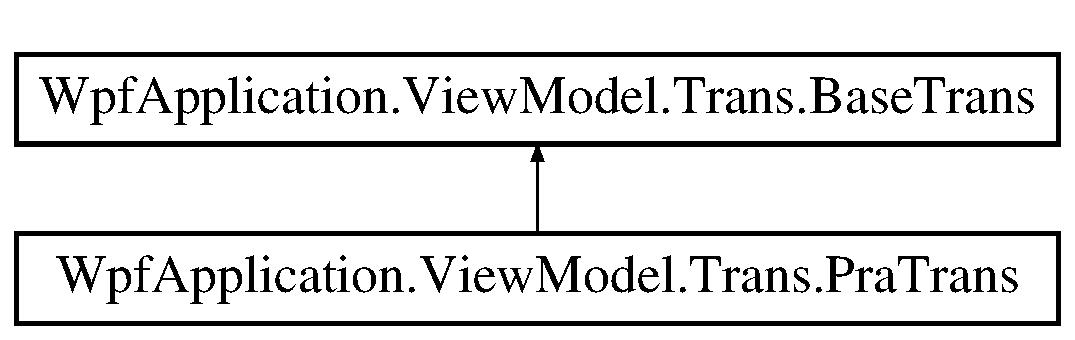
\includegraphics[height=2.000000cm]{class_wpf_application_1_1_view_model_1_1_trans_1_1_pra_trans}
\end{center}
\end{figure}
\subsection*{Public Member Functions}
\begin{DoxyCompactItemize}
\item 
\hyperlink{class_wpf_application_1_1_view_model_1_1_trans_1_1_pra_trans_aa5adc5e03191e8ba499f2aac5c9d6d09}{Pra\-Trans} (int mat, string \hyperlink{class_wpf_application_1_1_view_model_1_1_trans_1_1_pra_trans_a7440714237eda3b50d17c0c86f110527}{nom}, string \hyperlink{class_wpf_application_1_1_view_model_1_1_trans_1_1_pra_trans_aa0a1dc27ff028a606acbeaf3c00967e8}{prenom})
\item 
override string \hyperlink{class_wpf_application_1_1_view_model_1_1_trans_1_1_pra_trans_ad6aaa4787b9c62f1e8f4747269a4b9d7}{To\-String} ()
\item 
string \hyperlink{class_wpf_application_1_1_view_model_1_1_trans_1_1_pra_trans_ace508384ee863176bdfe40c1446dda47}{To\-Csv\-Row} ()
\begin{DoxyCompactList}\small\item\em Retourne une representation de l'instance sous forme d'une string, ligne d'un fichier C\-S\-V. Format\-: \char`\"{}col1;col2;col2\textbackslash{}n\char`\"{} \end{DoxyCompactList}\item 
override string \hyperlink{class_wpf_application_1_1_view_model_1_1_trans_1_1_pra_trans_a69e0d0034568e424fc88995a8bbfc06c}{get\-Class} ()
\end{DoxyCompactItemize}
\subsection*{Properties}
\begin{DoxyCompactItemize}
\item 
int \hyperlink{class_wpf_application_1_1_view_model_1_1_trans_1_1_pra_trans_a2789e23bae9ee1f522226f69231ad5c3}{matricule}\hspace{0.3cm}{\ttfamily  \mbox{[}get, set\mbox{]}}
\item 
string \hyperlink{class_wpf_application_1_1_view_model_1_1_trans_1_1_pra_trans_a7440714237eda3b50d17c0c86f110527}{nom}\hspace{0.3cm}{\ttfamily  \mbox{[}get, set\mbox{]}}
\item 
string \hyperlink{class_wpf_application_1_1_view_model_1_1_trans_1_1_pra_trans_aa0a1dc27ff028a606acbeaf3c00967e8}{prenom}\hspace{0.3cm}{\ttfamily  \mbox{[}get, set\mbox{]}}
\end{DoxyCompactItemize}


\subsection{Constructor \& Destructor Documentation}
\hypertarget{class_wpf_application_1_1_view_model_1_1_trans_1_1_pra_trans_aa5adc5e03191e8ba499f2aac5c9d6d09}{\index{Wpf\-Application\-::\-View\-Model\-::\-Trans\-::\-Pra\-Trans@{Wpf\-Application\-::\-View\-Model\-::\-Trans\-::\-Pra\-Trans}!Pra\-Trans@{Pra\-Trans}}
\index{Pra\-Trans@{Pra\-Trans}!WpfApplication::ViewModel::Trans::PraTrans@{Wpf\-Application\-::\-View\-Model\-::\-Trans\-::\-Pra\-Trans}}
\subsubsection[{Pra\-Trans}]{\setlength{\rightskip}{0pt plus 5cm}Wpf\-Application.\-View\-Model.\-Trans.\-Pra\-Trans.\-Pra\-Trans (
\begin{DoxyParamCaption}
\item[{int}]{mat, }
\item[{string}]{nom, }
\item[{string}]{prenom}
\end{DoxyParamCaption}
)}}\label{class_wpf_application_1_1_view_model_1_1_trans_1_1_pra_trans_aa5adc5e03191e8ba499f2aac5c9d6d09}


\subsection{Member Function Documentation}
\hypertarget{class_wpf_application_1_1_view_model_1_1_trans_1_1_pra_trans_a69e0d0034568e424fc88995a8bbfc06c}{\index{Wpf\-Application\-::\-View\-Model\-::\-Trans\-::\-Pra\-Trans@{Wpf\-Application\-::\-View\-Model\-::\-Trans\-::\-Pra\-Trans}!get\-Class@{get\-Class}}
\index{get\-Class@{get\-Class}!WpfApplication::ViewModel::Trans::PraTrans@{Wpf\-Application\-::\-View\-Model\-::\-Trans\-::\-Pra\-Trans}}
\subsubsection[{get\-Class}]{\setlength{\rightskip}{0pt plus 5cm}override string Wpf\-Application.\-View\-Model.\-Trans.\-Pra\-Trans.\-get\-Class (
\begin{DoxyParamCaption}
{}
\end{DoxyParamCaption}
)\hspace{0.3cm}{\ttfamily [virtual]}}}\label{class_wpf_application_1_1_view_model_1_1_trans_1_1_pra_trans_a69e0d0034568e424fc88995a8bbfc06c}


Reimplemented from \hyperlink{class_wpf_application_1_1_view_model_1_1_trans_1_1_base_trans_a9660be8cb25ed5d666eab9ddd10600aa}{Wpf\-Application.\-View\-Model.\-Trans.\-Base\-Trans}.

\hypertarget{class_wpf_application_1_1_view_model_1_1_trans_1_1_pra_trans_ace508384ee863176bdfe40c1446dda47}{\index{Wpf\-Application\-::\-View\-Model\-::\-Trans\-::\-Pra\-Trans@{Wpf\-Application\-::\-View\-Model\-::\-Trans\-::\-Pra\-Trans}!To\-Csv\-Row@{To\-Csv\-Row}}
\index{To\-Csv\-Row@{To\-Csv\-Row}!WpfApplication::ViewModel::Trans::PraTrans@{Wpf\-Application\-::\-View\-Model\-::\-Trans\-::\-Pra\-Trans}}
\subsubsection[{To\-Csv\-Row}]{\setlength{\rightskip}{0pt plus 5cm}string Wpf\-Application.\-View\-Model.\-Trans.\-Pra\-Trans.\-To\-Csv\-Row (
\begin{DoxyParamCaption}
{}
\end{DoxyParamCaption}
)}}\label{class_wpf_application_1_1_view_model_1_1_trans_1_1_pra_trans_ace508384ee863176bdfe40c1446dda47}


Retourne une representation de l'instance sous forme d'une string, ligne d'un fichier C\-S\-V. Format\-: \char`\"{}col1;col2;col2\textbackslash{}n\char`\"{} 

\begin{DoxyReturn}{Returns}
String, separee par des ';' et terminee par '\par
'
\end{DoxyReturn}
\hypertarget{class_wpf_application_1_1_view_model_1_1_trans_1_1_pra_trans_ad6aaa4787b9c62f1e8f4747269a4b9d7}{\index{Wpf\-Application\-::\-View\-Model\-::\-Trans\-::\-Pra\-Trans@{Wpf\-Application\-::\-View\-Model\-::\-Trans\-::\-Pra\-Trans}!To\-String@{To\-String}}
\index{To\-String@{To\-String}!WpfApplication::ViewModel::Trans::PraTrans@{Wpf\-Application\-::\-View\-Model\-::\-Trans\-::\-Pra\-Trans}}
\subsubsection[{To\-String}]{\setlength{\rightskip}{0pt plus 5cm}override string Wpf\-Application.\-View\-Model.\-Trans.\-Pra\-Trans.\-To\-String (
\begin{DoxyParamCaption}
{}
\end{DoxyParamCaption}
)}}\label{class_wpf_application_1_1_view_model_1_1_trans_1_1_pra_trans_ad6aaa4787b9c62f1e8f4747269a4b9d7}


\subsection{Property Documentation}
\hypertarget{class_wpf_application_1_1_view_model_1_1_trans_1_1_pra_trans_a2789e23bae9ee1f522226f69231ad5c3}{\index{Wpf\-Application\-::\-View\-Model\-::\-Trans\-::\-Pra\-Trans@{Wpf\-Application\-::\-View\-Model\-::\-Trans\-::\-Pra\-Trans}!matricule@{matricule}}
\index{matricule@{matricule}!WpfApplication::ViewModel::Trans::PraTrans@{Wpf\-Application\-::\-View\-Model\-::\-Trans\-::\-Pra\-Trans}}
\subsubsection[{matricule}]{\setlength{\rightskip}{0pt plus 5cm}int Wpf\-Application.\-View\-Model.\-Trans.\-Pra\-Trans.\-matricule\hspace{0.3cm}{\ttfamily [get]}, {\ttfamily [set]}}}\label{class_wpf_application_1_1_view_model_1_1_trans_1_1_pra_trans_a2789e23bae9ee1f522226f69231ad5c3}
\hypertarget{class_wpf_application_1_1_view_model_1_1_trans_1_1_pra_trans_a7440714237eda3b50d17c0c86f110527}{\index{Wpf\-Application\-::\-View\-Model\-::\-Trans\-::\-Pra\-Trans@{Wpf\-Application\-::\-View\-Model\-::\-Trans\-::\-Pra\-Trans}!nom@{nom}}
\index{nom@{nom}!WpfApplication::ViewModel::Trans::PraTrans@{Wpf\-Application\-::\-View\-Model\-::\-Trans\-::\-Pra\-Trans}}
\subsubsection[{nom}]{\setlength{\rightskip}{0pt plus 5cm}string Wpf\-Application.\-View\-Model.\-Trans.\-Pra\-Trans.\-nom\hspace{0.3cm}{\ttfamily [get]}, {\ttfamily [set]}}}\label{class_wpf_application_1_1_view_model_1_1_trans_1_1_pra_trans_a7440714237eda3b50d17c0c86f110527}
\hypertarget{class_wpf_application_1_1_view_model_1_1_trans_1_1_pra_trans_aa0a1dc27ff028a606acbeaf3c00967e8}{\index{Wpf\-Application\-::\-View\-Model\-::\-Trans\-::\-Pra\-Trans@{Wpf\-Application\-::\-View\-Model\-::\-Trans\-::\-Pra\-Trans}!prenom@{prenom}}
\index{prenom@{prenom}!WpfApplication::ViewModel::Trans::PraTrans@{Wpf\-Application\-::\-View\-Model\-::\-Trans\-::\-Pra\-Trans}}
\subsubsection[{prenom}]{\setlength{\rightskip}{0pt plus 5cm}string Wpf\-Application.\-View\-Model.\-Trans.\-Pra\-Trans.\-prenom\hspace{0.3cm}{\ttfamily [get]}, {\ttfamily [set]}}}\label{class_wpf_application_1_1_view_model_1_1_trans_1_1_pra_trans_aa0a1dc27ff028a606acbeaf3c00967e8}


The documentation for this class was generated from the following file\-:\begin{DoxyCompactItemize}
\item 
C\-:/\-Users/dju/\-Documents/\-Visual Studio 2012/\-Projects/\-P\-P\-E/\-P\-P\-E3/\-Wpf\-Application/\-View\-Model/\-Trans/\hyperlink{_prat_trans_8cs}{Prat\-Trans.\-cs}\end{DoxyCompactItemize}

\hypertarget{class_model_1_1_p_r_e_s_c_r_i_r_e}{\section{Model.\-P\-R\-E\-S\-C\-R\-I\-R\-E Class Reference}
\label{class_model_1_1_p_r_e_s_c_r_i_r_e}\index{Model.\-P\-R\-E\-S\-C\-R\-I\-R\-E@{Model.\-P\-R\-E\-S\-C\-R\-I\-R\-E}}
}


Aucune documentation sur les métadonnées n'est disponible.  


Inheritance diagram for Model.\-P\-R\-E\-S\-C\-R\-I\-R\-E\-:\begin{figure}[H]
\begin{center}
\leavevmode
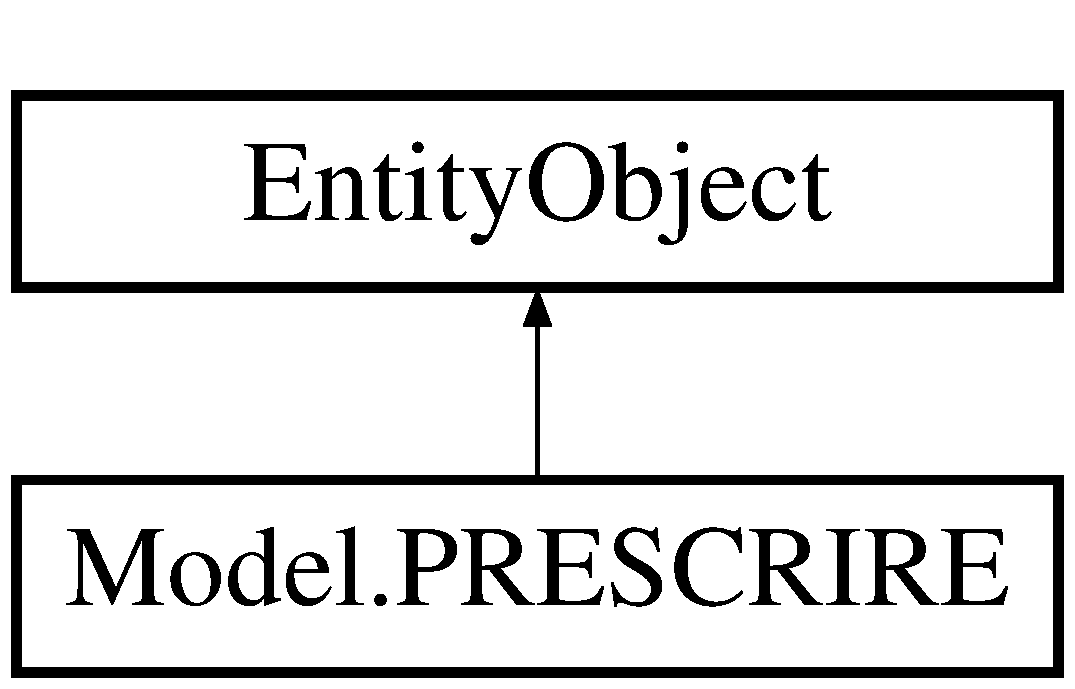
\includegraphics[height=2.000000cm]{class_model_1_1_p_r_e_s_c_r_i_r_e}
\end{center}
\end{figure}
\subsection*{Static Public Member Functions}
\begin{DoxyCompactItemize}
\item 
static \hyperlink{class_model_1_1_p_r_e_s_c_r_i_r_e}{P\-R\-E\-S\-C\-R\-I\-R\-E} \hyperlink{class_model_1_1_p_r_e_s_c_r_i_r_e_aff6d043851452306b1da12b746253874}{Create\-P\-R\-E\-S\-C\-R\-I\-R\-E} (global\-::\-System.\-String \hyperlink{class_model_1_1_p_r_e_s_c_r_i_r_e_a9b74be9f296f7872642b907acd30f857}{depot\-\_\-legal\-\_\-prescr}, global\-::\-System.\-Int32 \hyperlink{class_model_1_1_p_r_e_s_c_r_i_r_e_a7d149f06b9852794be2b5246e0bedaf3}{code\-\_\-dosage}, global\-::\-System.\-Int32 \hyperlink{class_model_1_1_p_r_e_s_c_r_i_r_e_adb817829898cdf62b98e9e3ac19f43ae}{code\-\_\-individu}, global\-::\-System.\-String \hyperlink{class_model_1_1_p_r_e_s_c_r_i_r_e_a1cf3de1e828418d612305ac1a6c62c04}{posologie})
\begin{DoxyCompactList}\small\item\em Créez un nouvel objet \hyperlink{class_model_1_1_p_r_e_s_c_r_i_r_e}{P\-R\-E\-S\-C\-R\-I\-R\-E}. \end{DoxyCompactList}\end{DoxyCompactItemize}
\subsection*{Properties}
\begin{DoxyCompactItemize}
\item 
global\-::\-System.\-String \hyperlink{class_model_1_1_p_r_e_s_c_r_i_r_e_a9b74be9f296f7872642b907acd30f857}{depot\-\_\-legal\-\_\-prescr}\hspace{0.3cm}{\ttfamily  \mbox{[}get, set\mbox{]}}
\begin{DoxyCompactList}\small\item\em Aucune documentation sur les métadonnées n'est disponible. \end{DoxyCompactList}\item 
global\-::\-System.\-Int32 \hyperlink{class_model_1_1_p_r_e_s_c_r_i_r_e_a7d149f06b9852794be2b5246e0bedaf3}{code\-\_\-dosage}\hspace{0.3cm}{\ttfamily  \mbox{[}get, set\mbox{]}}
\begin{DoxyCompactList}\small\item\em Aucune documentation sur les métadonnées n'est disponible. \end{DoxyCompactList}\item 
global\-::\-System.\-Int32 \hyperlink{class_model_1_1_p_r_e_s_c_r_i_r_e_adb817829898cdf62b98e9e3ac19f43ae}{code\-\_\-individu}\hspace{0.3cm}{\ttfamily  \mbox{[}get, set\mbox{]}}
\begin{DoxyCompactList}\small\item\em Aucune documentation sur les métadonnées n'est disponible. \end{DoxyCompactList}\item 
global\-::\-System.\-String \hyperlink{class_model_1_1_p_r_e_s_c_r_i_r_e_a1cf3de1e828418d612305ac1a6c62c04}{posologie}\hspace{0.3cm}{\ttfamily  \mbox{[}get, set\mbox{]}}
\begin{DoxyCompactList}\small\item\em Aucune documentation sur les métadonnées n'est disponible. \end{DoxyCompactList}\item 
\hyperlink{class_model_1_1_d_o_s_a_g_e}{D\-O\-S\-A\-G\-E} \hyperlink{class_model_1_1_p_r_e_s_c_r_i_r_e_a1af2abaa082cabb9c53e3e16e1aab6ba}{D\-O\-S\-A\-G\-E}\hspace{0.3cm}{\ttfamily  \mbox{[}get, set\mbox{]}}
\begin{DoxyCompactList}\small\item\em Aucune documentation sur les métadonnées n'est disponible. \end{DoxyCompactList}\item 
Entity\-Reference$<$ \hyperlink{class_model_1_1_d_o_s_a_g_e}{D\-O\-S\-A\-G\-E} $>$ \hyperlink{class_model_1_1_p_r_e_s_c_r_i_r_e_a5b8a8b554f87bbf94855802f7bfb1815}{D\-O\-S\-A\-G\-E\-Reference}\hspace{0.3cm}{\ttfamily  \mbox{[}get, set\mbox{]}}
\begin{DoxyCompactList}\small\item\em Aucune documentation sur les métadonnées n'est disponible. \end{DoxyCompactList}\item 
\hyperlink{class_model_1_1_m_e_d_i_c_a_m_e_n_t}{M\-E\-D\-I\-C\-A\-M\-E\-N\-T} \hyperlink{class_model_1_1_p_r_e_s_c_r_i_r_e_ac2d56f6ccfeff98e9e4e75ebeb8a183b}{M\-E\-D\-I\-C\-A\-M\-E\-N\-T}\hspace{0.3cm}{\ttfamily  \mbox{[}get, set\mbox{]}}
\begin{DoxyCompactList}\small\item\em Aucune documentation sur les métadonnées n'est disponible. \end{DoxyCompactList}\item 
Entity\-Reference$<$ \hyperlink{class_model_1_1_m_e_d_i_c_a_m_e_n_t}{M\-E\-D\-I\-C\-A\-M\-E\-N\-T} $>$ \hyperlink{class_model_1_1_p_r_e_s_c_r_i_r_e_ae6eb0aa552e585dcd17936b993947f0c}{M\-E\-D\-I\-C\-A\-M\-E\-N\-T\-Reference}\hspace{0.3cm}{\ttfamily  \mbox{[}get, set\mbox{]}}
\begin{DoxyCompactList}\small\item\em Aucune documentation sur les métadonnées n'est disponible. \end{DoxyCompactList}\item 
\hyperlink{class_model_1_1_t_y_p_e___i_n_d_i_v_i_d_u}{T\-Y\-P\-E\-\_\-\-I\-N\-D\-I\-V\-I\-D\-U} \hyperlink{class_model_1_1_p_r_e_s_c_r_i_r_e_a894c92b24554d0819f2ac129895a7980}{T\-Y\-P\-E\-\_\-\-I\-N\-D\-I\-V\-I\-D\-U}\hspace{0.3cm}{\ttfamily  \mbox{[}get, set\mbox{]}}
\begin{DoxyCompactList}\small\item\em Aucune documentation sur les métadonnées n'est disponible. \end{DoxyCompactList}\item 
Entity\-Reference$<$ \hyperlink{class_model_1_1_t_y_p_e___i_n_d_i_v_i_d_u}{T\-Y\-P\-E\-\_\-\-I\-N\-D\-I\-V\-I\-D\-U} $>$ \hyperlink{class_model_1_1_p_r_e_s_c_r_i_r_e_aa58692d5b4e38e34b13f7df01fdcb321}{T\-Y\-P\-E\-\_\-\-I\-N\-D\-I\-V\-I\-D\-U\-Reference}\hspace{0.3cm}{\ttfamily  \mbox{[}get, set\mbox{]}}
\begin{DoxyCompactList}\small\item\em Aucune documentation sur les métadonnées n'est disponible. \end{DoxyCompactList}\end{DoxyCompactItemize}


\subsection{Detailed Description}
Aucune documentation sur les métadonnées n'est disponible. 



\subsection{Member Function Documentation}
\hypertarget{class_model_1_1_p_r_e_s_c_r_i_r_e_aff6d043851452306b1da12b746253874}{\index{Model\-::\-P\-R\-E\-S\-C\-R\-I\-R\-E@{Model\-::\-P\-R\-E\-S\-C\-R\-I\-R\-E}!Create\-P\-R\-E\-S\-C\-R\-I\-R\-E@{Create\-P\-R\-E\-S\-C\-R\-I\-R\-E}}
\index{Create\-P\-R\-E\-S\-C\-R\-I\-R\-E@{Create\-P\-R\-E\-S\-C\-R\-I\-R\-E}!Model::PRESCRIRE@{Model\-::\-P\-R\-E\-S\-C\-R\-I\-R\-E}}
\subsubsection[{Create\-P\-R\-E\-S\-C\-R\-I\-R\-E}]{\setlength{\rightskip}{0pt plus 5cm}static {\bf P\-R\-E\-S\-C\-R\-I\-R\-E} Model.\-P\-R\-E\-S\-C\-R\-I\-R\-E.\-Create\-P\-R\-E\-S\-C\-R\-I\-R\-E (
\begin{DoxyParamCaption}
\item[{global\-::\-System.\-String}]{depot\-\_\-legal\-\_\-prescr, }
\item[{global\-::\-System.\-Int32}]{code\-\_\-dosage, }
\item[{global\-::\-System.\-Int32}]{code\-\_\-individu, }
\item[{global\-::\-System.\-String}]{posologie}
\end{DoxyParamCaption}
)\hspace{0.3cm}{\ttfamily [static]}}}\label{class_model_1_1_p_r_e_s_c_r_i_r_e_aff6d043851452306b1da12b746253874}


Créez un nouvel objet \hyperlink{class_model_1_1_p_r_e_s_c_r_i_r_e}{P\-R\-E\-S\-C\-R\-I\-R\-E}. 


\begin{DoxyParams}{Parameters}
{\em depot\-\_\-legal\-\_\-prescr} & Valeur initiale de la propriété depot\-\_\-legal\-\_\-prescr.\\
\hline
{\em code\-\_\-dosage} & Valeur initiale de la propriété code\-\_\-dosage.\\
\hline
{\em code\-\_\-individu} & Valeur initiale de la propriété code\-\_\-individu.\\
\hline
{\em posologie} & Valeur initiale de la propriété posologie.\\
\hline
\end{DoxyParams}


\subsection{Property Documentation}
\hypertarget{class_model_1_1_p_r_e_s_c_r_i_r_e_a7d149f06b9852794be2b5246e0bedaf3}{\index{Model\-::\-P\-R\-E\-S\-C\-R\-I\-R\-E@{Model\-::\-P\-R\-E\-S\-C\-R\-I\-R\-E}!code\-\_\-dosage@{code\-\_\-dosage}}
\index{code\-\_\-dosage@{code\-\_\-dosage}!Model::PRESCRIRE@{Model\-::\-P\-R\-E\-S\-C\-R\-I\-R\-E}}
\subsubsection[{code\-\_\-dosage}]{\setlength{\rightskip}{0pt plus 5cm}global.\-System.\-Int32 Model.\-P\-R\-E\-S\-C\-R\-I\-R\-E.\-code\-\_\-dosage\hspace{0.3cm}{\ttfamily [get]}, {\ttfamily [set]}}}\label{class_model_1_1_p_r_e_s_c_r_i_r_e_a7d149f06b9852794be2b5246e0bedaf3}


Aucune documentation sur les métadonnées n'est disponible. 

\hypertarget{class_model_1_1_p_r_e_s_c_r_i_r_e_adb817829898cdf62b98e9e3ac19f43ae}{\index{Model\-::\-P\-R\-E\-S\-C\-R\-I\-R\-E@{Model\-::\-P\-R\-E\-S\-C\-R\-I\-R\-E}!code\-\_\-individu@{code\-\_\-individu}}
\index{code\-\_\-individu@{code\-\_\-individu}!Model::PRESCRIRE@{Model\-::\-P\-R\-E\-S\-C\-R\-I\-R\-E}}
\subsubsection[{code\-\_\-individu}]{\setlength{\rightskip}{0pt plus 5cm}global.\-System.\-Int32 Model.\-P\-R\-E\-S\-C\-R\-I\-R\-E.\-code\-\_\-individu\hspace{0.3cm}{\ttfamily [get]}, {\ttfamily [set]}}}\label{class_model_1_1_p_r_e_s_c_r_i_r_e_adb817829898cdf62b98e9e3ac19f43ae}


Aucune documentation sur les métadonnées n'est disponible. 

\hypertarget{class_model_1_1_p_r_e_s_c_r_i_r_e_a9b74be9f296f7872642b907acd30f857}{\index{Model\-::\-P\-R\-E\-S\-C\-R\-I\-R\-E@{Model\-::\-P\-R\-E\-S\-C\-R\-I\-R\-E}!depot\-\_\-legal\-\_\-prescr@{depot\-\_\-legal\-\_\-prescr}}
\index{depot\-\_\-legal\-\_\-prescr@{depot\-\_\-legal\-\_\-prescr}!Model::PRESCRIRE@{Model\-::\-P\-R\-E\-S\-C\-R\-I\-R\-E}}
\subsubsection[{depot\-\_\-legal\-\_\-prescr}]{\setlength{\rightskip}{0pt plus 5cm}global.\-System.\-String Model.\-P\-R\-E\-S\-C\-R\-I\-R\-E.\-depot\-\_\-legal\-\_\-prescr\hspace{0.3cm}{\ttfamily [get]}, {\ttfamily [set]}}}\label{class_model_1_1_p_r_e_s_c_r_i_r_e_a9b74be9f296f7872642b907acd30f857}


Aucune documentation sur les métadonnées n'est disponible. 

\hypertarget{class_model_1_1_p_r_e_s_c_r_i_r_e_a1af2abaa082cabb9c53e3e16e1aab6ba}{\index{Model\-::\-P\-R\-E\-S\-C\-R\-I\-R\-E@{Model\-::\-P\-R\-E\-S\-C\-R\-I\-R\-E}!D\-O\-S\-A\-G\-E@{D\-O\-S\-A\-G\-E}}
\index{D\-O\-S\-A\-G\-E@{D\-O\-S\-A\-G\-E}!Model::PRESCRIRE@{Model\-::\-P\-R\-E\-S\-C\-R\-I\-R\-E}}
\subsubsection[{D\-O\-S\-A\-G\-E}]{\setlength{\rightskip}{0pt plus 5cm}{\bf D\-O\-S\-A\-G\-E} Model.\-P\-R\-E\-S\-C\-R\-I\-R\-E.\-D\-O\-S\-A\-G\-E\hspace{0.3cm}{\ttfamily [get]}, {\ttfamily [set]}}}\label{class_model_1_1_p_r_e_s_c_r_i_r_e_a1af2abaa082cabb9c53e3e16e1aab6ba}


Aucune documentation sur les métadonnées n'est disponible. 

\hypertarget{class_model_1_1_p_r_e_s_c_r_i_r_e_a5b8a8b554f87bbf94855802f7bfb1815}{\index{Model\-::\-P\-R\-E\-S\-C\-R\-I\-R\-E@{Model\-::\-P\-R\-E\-S\-C\-R\-I\-R\-E}!D\-O\-S\-A\-G\-E\-Reference@{D\-O\-S\-A\-G\-E\-Reference}}
\index{D\-O\-S\-A\-G\-E\-Reference@{D\-O\-S\-A\-G\-E\-Reference}!Model::PRESCRIRE@{Model\-::\-P\-R\-E\-S\-C\-R\-I\-R\-E}}
\subsubsection[{D\-O\-S\-A\-G\-E\-Reference}]{\setlength{\rightskip}{0pt plus 5cm}Entity\-Reference$<${\bf D\-O\-S\-A\-G\-E}$>$ Model.\-P\-R\-E\-S\-C\-R\-I\-R\-E.\-D\-O\-S\-A\-G\-E\-Reference\hspace{0.3cm}{\ttfamily [get]}, {\ttfamily [set]}}}\label{class_model_1_1_p_r_e_s_c_r_i_r_e_a5b8a8b554f87bbf94855802f7bfb1815}


Aucune documentation sur les métadonnées n'est disponible. 

\hypertarget{class_model_1_1_p_r_e_s_c_r_i_r_e_ac2d56f6ccfeff98e9e4e75ebeb8a183b}{\index{Model\-::\-P\-R\-E\-S\-C\-R\-I\-R\-E@{Model\-::\-P\-R\-E\-S\-C\-R\-I\-R\-E}!M\-E\-D\-I\-C\-A\-M\-E\-N\-T@{M\-E\-D\-I\-C\-A\-M\-E\-N\-T}}
\index{M\-E\-D\-I\-C\-A\-M\-E\-N\-T@{M\-E\-D\-I\-C\-A\-M\-E\-N\-T}!Model::PRESCRIRE@{Model\-::\-P\-R\-E\-S\-C\-R\-I\-R\-E}}
\subsubsection[{M\-E\-D\-I\-C\-A\-M\-E\-N\-T}]{\setlength{\rightskip}{0pt plus 5cm}{\bf M\-E\-D\-I\-C\-A\-M\-E\-N\-T} Model.\-P\-R\-E\-S\-C\-R\-I\-R\-E.\-M\-E\-D\-I\-C\-A\-M\-E\-N\-T\hspace{0.3cm}{\ttfamily [get]}, {\ttfamily [set]}}}\label{class_model_1_1_p_r_e_s_c_r_i_r_e_ac2d56f6ccfeff98e9e4e75ebeb8a183b}


Aucune documentation sur les métadonnées n'est disponible. 

\hypertarget{class_model_1_1_p_r_e_s_c_r_i_r_e_ae6eb0aa552e585dcd17936b993947f0c}{\index{Model\-::\-P\-R\-E\-S\-C\-R\-I\-R\-E@{Model\-::\-P\-R\-E\-S\-C\-R\-I\-R\-E}!M\-E\-D\-I\-C\-A\-M\-E\-N\-T\-Reference@{M\-E\-D\-I\-C\-A\-M\-E\-N\-T\-Reference}}
\index{M\-E\-D\-I\-C\-A\-M\-E\-N\-T\-Reference@{M\-E\-D\-I\-C\-A\-M\-E\-N\-T\-Reference}!Model::PRESCRIRE@{Model\-::\-P\-R\-E\-S\-C\-R\-I\-R\-E}}
\subsubsection[{M\-E\-D\-I\-C\-A\-M\-E\-N\-T\-Reference}]{\setlength{\rightskip}{0pt plus 5cm}Entity\-Reference$<${\bf M\-E\-D\-I\-C\-A\-M\-E\-N\-T}$>$ Model.\-P\-R\-E\-S\-C\-R\-I\-R\-E.\-M\-E\-D\-I\-C\-A\-M\-E\-N\-T\-Reference\hspace{0.3cm}{\ttfamily [get]}, {\ttfamily [set]}}}\label{class_model_1_1_p_r_e_s_c_r_i_r_e_ae6eb0aa552e585dcd17936b993947f0c}


Aucune documentation sur les métadonnées n'est disponible. 

\hypertarget{class_model_1_1_p_r_e_s_c_r_i_r_e_a1cf3de1e828418d612305ac1a6c62c04}{\index{Model\-::\-P\-R\-E\-S\-C\-R\-I\-R\-E@{Model\-::\-P\-R\-E\-S\-C\-R\-I\-R\-E}!posologie@{posologie}}
\index{posologie@{posologie}!Model::PRESCRIRE@{Model\-::\-P\-R\-E\-S\-C\-R\-I\-R\-E}}
\subsubsection[{posologie}]{\setlength{\rightskip}{0pt plus 5cm}global.\-System.\-String Model.\-P\-R\-E\-S\-C\-R\-I\-R\-E.\-posologie\hspace{0.3cm}{\ttfamily [get]}, {\ttfamily [set]}}}\label{class_model_1_1_p_r_e_s_c_r_i_r_e_a1cf3de1e828418d612305ac1a6c62c04}


Aucune documentation sur les métadonnées n'est disponible. 

\hypertarget{class_model_1_1_p_r_e_s_c_r_i_r_e_a894c92b24554d0819f2ac129895a7980}{\index{Model\-::\-P\-R\-E\-S\-C\-R\-I\-R\-E@{Model\-::\-P\-R\-E\-S\-C\-R\-I\-R\-E}!T\-Y\-P\-E\-\_\-\-I\-N\-D\-I\-V\-I\-D\-U@{T\-Y\-P\-E\-\_\-\-I\-N\-D\-I\-V\-I\-D\-U}}
\index{T\-Y\-P\-E\-\_\-\-I\-N\-D\-I\-V\-I\-D\-U@{T\-Y\-P\-E\-\_\-\-I\-N\-D\-I\-V\-I\-D\-U}!Model::PRESCRIRE@{Model\-::\-P\-R\-E\-S\-C\-R\-I\-R\-E}}
\subsubsection[{T\-Y\-P\-E\-\_\-\-I\-N\-D\-I\-V\-I\-D\-U}]{\setlength{\rightskip}{0pt plus 5cm}{\bf T\-Y\-P\-E\-\_\-\-I\-N\-D\-I\-V\-I\-D\-U} Model.\-P\-R\-E\-S\-C\-R\-I\-R\-E.\-T\-Y\-P\-E\-\_\-\-I\-N\-D\-I\-V\-I\-D\-U\hspace{0.3cm}{\ttfamily [get]}, {\ttfamily [set]}}}\label{class_model_1_1_p_r_e_s_c_r_i_r_e_a894c92b24554d0819f2ac129895a7980}


Aucune documentation sur les métadonnées n'est disponible. 

\hypertarget{class_model_1_1_p_r_e_s_c_r_i_r_e_aa58692d5b4e38e34b13f7df01fdcb321}{\index{Model\-::\-P\-R\-E\-S\-C\-R\-I\-R\-E@{Model\-::\-P\-R\-E\-S\-C\-R\-I\-R\-E}!T\-Y\-P\-E\-\_\-\-I\-N\-D\-I\-V\-I\-D\-U\-Reference@{T\-Y\-P\-E\-\_\-\-I\-N\-D\-I\-V\-I\-D\-U\-Reference}}
\index{T\-Y\-P\-E\-\_\-\-I\-N\-D\-I\-V\-I\-D\-U\-Reference@{T\-Y\-P\-E\-\_\-\-I\-N\-D\-I\-V\-I\-D\-U\-Reference}!Model::PRESCRIRE@{Model\-::\-P\-R\-E\-S\-C\-R\-I\-R\-E}}
\subsubsection[{T\-Y\-P\-E\-\_\-\-I\-N\-D\-I\-V\-I\-D\-U\-Reference}]{\setlength{\rightskip}{0pt plus 5cm}Entity\-Reference$<${\bf T\-Y\-P\-E\-\_\-\-I\-N\-D\-I\-V\-I\-D\-U}$>$ Model.\-P\-R\-E\-S\-C\-R\-I\-R\-E.\-T\-Y\-P\-E\-\_\-\-I\-N\-D\-I\-V\-I\-D\-U\-Reference\hspace{0.3cm}{\ttfamily [get]}, {\ttfamily [set]}}}\label{class_model_1_1_p_r_e_s_c_r_i_r_e_aa58692d5b4e38e34b13f7df01fdcb321}


Aucune documentation sur les métadonnées n'est disponible. 



The documentation for this class was generated from the following file\-:\begin{DoxyCompactItemize}
\item 
C\-:/\-Users/dju/\-Documents/\-Visual Studio 2012/\-Projects/\-P\-P\-E/\-P\-P\-E3/\-Model/\hyperlink{_model_bdd_sio_8_designer_8cs}{Model\-Bdd\-Sio.\-Designer.\-cs}\end{DoxyCompactItemize}

\hypertarget{class_model_1_1_p_r_e_s_e_n_t_a_t_i_o_n}{\section{Model.\-P\-R\-E\-S\-E\-N\-T\-A\-T\-I\-O\-N Class Reference}
\label{class_model_1_1_p_r_e_s_e_n_t_a_t_i_o_n}\index{Model.\-P\-R\-E\-S\-E\-N\-T\-A\-T\-I\-O\-N@{Model.\-P\-R\-E\-S\-E\-N\-T\-A\-T\-I\-O\-N}}
}


Aucune documentation sur les métadonnées n'est disponible.  


Inheritance diagram for Model.\-P\-R\-E\-S\-E\-N\-T\-A\-T\-I\-O\-N\-:\begin{figure}[H]
\begin{center}
\leavevmode
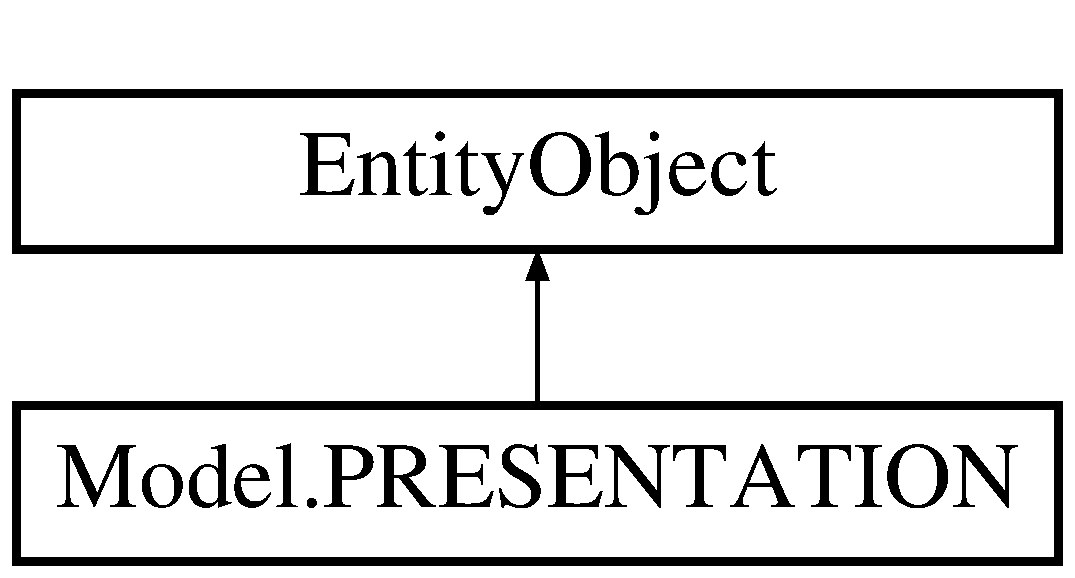
\includegraphics[height=2.000000cm]{class_model_1_1_p_r_e_s_e_n_t_a_t_i_o_n}
\end{center}
\end{figure}
\subsection*{Static Public Member Functions}
\begin{DoxyCompactItemize}
\item 
static \hyperlink{class_model_1_1_p_r_e_s_e_n_t_a_t_i_o_n}{P\-R\-E\-S\-E\-N\-T\-A\-T\-I\-O\-N} \hyperlink{class_model_1_1_p_r_e_s_e_n_t_a_t_i_o_n_a2d14b8c142e8bc7e1079e977aca12951}{Create\-P\-R\-E\-S\-E\-N\-T\-A\-T\-I\-O\-N} (global\-::\-System.\-Int32 \hyperlink{class_model_1_1_p_r_e_s_e_n_t_a_t_i_o_n_a97c7cbefa08736b44382aec5dda9adf4}{code\-\_\-present}, global\-::\-System.\-String \hyperlink{class_model_1_1_p_r_e_s_e_n_t_a_t_i_o_n_ae64c2be728fa1e6dbd1a5766e4453d07}{libelle\-\_\-present}, global\-::\-System.\-String \hyperlink{class_model_1_1_p_r_e_s_e_n_t_a_t_i_o_n_a9e2fa4b05a5ce426e1c1cc8ec44b25bc}{depot\-\_\-legal\-\_\-present})
\begin{DoxyCompactList}\small\item\em Créez un nouvel objet \hyperlink{class_model_1_1_p_r_e_s_e_n_t_a_t_i_o_n}{P\-R\-E\-S\-E\-N\-T\-A\-T\-I\-O\-N}. \end{DoxyCompactList}\end{DoxyCompactItemize}
\subsection*{Properties}
\begin{DoxyCompactItemize}
\item 
global\-::\-System.\-Int32 \hyperlink{class_model_1_1_p_r_e_s_e_n_t_a_t_i_o_n_a97c7cbefa08736b44382aec5dda9adf4}{code\-\_\-present}\hspace{0.3cm}{\ttfamily  \mbox{[}get, set\mbox{]}}
\begin{DoxyCompactList}\small\item\em Aucune documentation sur les métadonnées n'est disponible. \end{DoxyCompactList}\item 
global\-::\-System.\-String \hyperlink{class_model_1_1_p_r_e_s_e_n_t_a_t_i_o_n_ae64c2be728fa1e6dbd1a5766e4453d07}{libelle\-\_\-present}\hspace{0.3cm}{\ttfamily  \mbox{[}get, set\mbox{]}}
\begin{DoxyCompactList}\small\item\em Aucune documentation sur les métadonnées n'est disponible. \end{DoxyCompactList}\item 
global\-::\-System.\-String \hyperlink{class_model_1_1_p_r_e_s_e_n_t_a_t_i_o_n_a9e2fa4b05a5ce426e1c1cc8ec44b25bc}{depot\-\_\-legal\-\_\-present}\hspace{0.3cm}{\ttfamily  \mbox{[}get, set\mbox{]}}
\begin{DoxyCompactList}\small\item\em Aucune documentation sur les métadonnées n'est disponible. \end{DoxyCompactList}\item 
Entity\-Collection$<$ \hyperlink{class_model_1_1_m_e_d_i_c_a_m_e_n_t}{M\-E\-D\-I\-C\-A\-M\-E\-N\-T} $>$ \hyperlink{class_model_1_1_p_r_e_s_e_n_t_a_t_i_o_n_a0b3e3f0cdd8d574cb35b28ee097ab0af}{M\-E\-D\-I\-C\-A\-M\-E\-N\-T}\hspace{0.3cm}{\ttfamily  \mbox{[}get, set\mbox{]}}
\begin{DoxyCompactList}\small\item\em Aucune documentation sur les métadonnées n'est disponible. \end{DoxyCompactList}\end{DoxyCompactItemize}


\subsection{Detailed Description}
Aucune documentation sur les métadonnées n'est disponible. 



\subsection{Member Function Documentation}
\hypertarget{class_model_1_1_p_r_e_s_e_n_t_a_t_i_o_n_a2d14b8c142e8bc7e1079e977aca12951}{\index{Model\-::\-P\-R\-E\-S\-E\-N\-T\-A\-T\-I\-O\-N@{Model\-::\-P\-R\-E\-S\-E\-N\-T\-A\-T\-I\-O\-N}!Create\-P\-R\-E\-S\-E\-N\-T\-A\-T\-I\-O\-N@{Create\-P\-R\-E\-S\-E\-N\-T\-A\-T\-I\-O\-N}}
\index{Create\-P\-R\-E\-S\-E\-N\-T\-A\-T\-I\-O\-N@{Create\-P\-R\-E\-S\-E\-N\-T\-A\-T\-I\-O\-N}!Model::PRESENTATION@{Model\-::\-P\-R\-E\-S\-E\-N\-T\-A\-T\-I\-O\-N}}
\subsubsection[{Create\-P\-R\-E\-S\-E\-N\-T\-A\-T\-I\-O\-N}]{\setlength{\rightskip}{0pt plus 5cm}static {\bf P\-R\-E\-S\-E\-N\-T\-A\-T\-I\-O\-N} Model.\-P\-R\-E\-S\-E\-N\-T\-A\-T\-I\-O\-N.\-Create\-P\-R\-E\-S\-E\-N\-T\-A\-T\-I\-O\-N (
\begin{DoxyParamCaption}
\item[{global\-::\-System.\-Int32}]{code\-\_\-present, }
\item[{global\-::\-System.\-String}]{libelle\-\_\-present, }
\item[{global\-::\-System.\-String}]{depot\-\_\-legal\-\_\-present}
\end{DoxyParamCaption}
)\hspace{0.3cm}{\ttfamily [static]}}}\label{class_model_1_1_p_r_e_s_e_n_t_a_t_i_o_n_a2d14b8c142e8bc7e1079e977aca12951}


Créez un nouvel objet \hyperlink{class_model_1_1_p_r_e_s_e_n_t_a_t_i_o_n}{P\-R\-E\-S\-E\-N\-T\-A\-T\-I\-O\-N}. 


\begin{DoxyParams}{Parameters}
{\em code\-\_\-present} & Valeur initiale de la propriété code\-\_\-present.\\
\hline
{\em libelle\-\_\-present} & Valeur initiale de la propriété libelle\-\_\-present.\\
\hline
{\em depot\-\_\-legal\-\_\-present} & Valeur initiale de la propriété depot\-\_\-legal\-\_\-present.\\
\hline
\end{DoxyParams}


\subsection{Property Documentation}
\hypertarget{class_model_1_1_p_r_e_s_e_n_t_a_t_i_o_n_a97c7cbefa08736b44382aec5dda9adf4}{\index{Model\-::\-P\-R\-E\-S\-E\-N\-T\-A\-T\-I\-O\-N@{Model\-::\-P\-R\-E\-S\-E\-N\-T\-A\-T\-I\-O\-N}!code\-\_\-present@{code\-\_\-present}}
\index{code\-\_\-present@{code\-\_\-present}!Model::PRESENTATION@{Model\-::\-P\-R\-E\-S\-E\-N\-T\-A\-T\-I\-O\-N}}
\subsubsection[{code\-\_\-present}]{\setlength{\rightskip}{0pt plus 5cm}global.\-System.\-Int32 Model.\-P\-R\-E\-S\-E\-N\-T\-A\-T\-I\-O\-N.\-code\-\_\-present\hspace{0.3cm}{\ttfamily [get]}, {\ttfamily [set]}}}\label{class_model_1_1_p_r_e_s_e_n_t_a_t_i_o_n_a97c7cbefa08736b44382aec5dda9adf4}


Aucune documentation sur les métadonnées n'est disponible. 

\hypertarget{class_model_1_1_p_r_e_s_e_n_t_a_t_i_o_n_a9e2fa4b05a5ce426e1c1cc8ec44b25bc}{\index{Model\-::\-P\-R\-E\-S\-E\-N\-T\-A\-T\-I\-O\-N@{Model\-::\-P\-R\-E\-S\-E\-N\-T\-A\-T\-I\-O\-N}!depot\-\_\-legal\-\_\-present@{depot\-\_\-legal\-\_\-present}}
\index{depot\-\_\-legal\-\_\-present@{depot\-\_\-legal\-\_\-present}!Model::PRESENTATION@{Model\-::\-P\-R\-E\-S\-E\-N\-T\-A\-T\-I\-O\-N}}
\subsubsection[{depot\-\_\-legal\-\_\-present}]{\setlength{\rightskip}{0pt plus 5cm}global.\-System.\-String Model.\-P\-R\-E\-S\-E\-N\-T\-A\-T\-I\-O\-N.\-depot\-\_\-legal\-\_\-present\hspace{0.3cm}{\ttfamily [get]}, {\ttfamily [set]}}}\label{class_model_1_1_p_r_e_s_e_n_t_a_t_i_o_n_a9e2fa4b05a5ce426e1c1cc8ec44b25bc}


Aucune documentation sur les métadonnées n'est disponible. 

\hypertarget{class_model_1_1_p_r_e_s_e_n_t_a_t_i_o_n_ae64c2be728fa1e6dbd1a5766e4453d07}{\index{Model\-::\-P\-R\-E\-S\-E\-N\-T\-A\-T\-I\-O\-N@{Model\-::\-P\-R\-E\-S\-E\-N\-T\-A\-T\-I\-O\-N}!libelle\-\_\-present@{libelle\-\_\-present}}
\index{libelle\-\_\-present@{libelle\-\_\-present}!Model::PRESENTATION@{Model\-::\-P\-R\-E\-S\-E\-N\-T\-A\-T\-I\-O\-N}}
\subsubsection[{libelle\-\_\-present}]{\setlength{\rightskip}{0pt plus 5cm}global.\-System.\-String Model.\-P\-R\-E\-S\-E\-N\-T\-A\-T\-I\-O\-N.\-libelle\-\_\-present\hspace{0.3cm}{\ttfamily [get]}, {\ttfamily [set]}}}\label{class_model_1_1_p_r_e_s_e_n_t_a_t_i_o_n_ae64c2be728fa1e6dbd1a5766e4453d07}


Aucune documentation sur les métadonnées n'est disponible. 

\hypertarget{class_model_1_1_p_r_e_s_e_n_t_a_t_i_o_n_a0b3e3f0cdd8d574cb35b28ee097ab0af}{\index{Model\-::\-P\-R\-E\-S\-E\-N\-T\-A\-T\-I\-O\-N@{Model\-::\-P\-R\-E\-S\-E\-N\-T\-A\-T\-I\-O\-N}!M\-E\-D\-I\-C\-A\-M\-E\-N\-T@{M\-E\-D\-I\-C\-A\-M\-E\-N\-T}}
\index{M\-E\-D\-I\-C\-A\-M\-E\-N\-T@{M\-E\-D\-I\-C\-A\-M\-E\-N\-T}!Model::PRESENTATION@{Model\-::\-P\-R\-E\-S\-E\-N\-T\-A\-T\-I\-O\-N}}
\subsubsection[{M\-E\-D\-I\-C\-A\-M\-E\-N\-T}]{\setlength{\rightskip}{0pt plus 5cm}Entity\-Collection$<${\bf M\-E\-D\-I\-C\-A\-M\-E\-N\-T}$>$ Model.\-P\-R\-E\-S\-E\-N\-T\-A\-T\-I\-O\-N.\-M\-E\-D\-I\-C\-A\-M\-E\-N\-T\hspace{0.3cm}{\ttfamily [get]}, {\ttfamily [set]}}}\label{class_model_1_1_p_r_e_s_e_n_t_a_t_i_o_n_a0b3e3f0cdd8d574cb35b28ee097ab0af}


Aucune documentation sur les métadonnées n'est disponible. 



The documentation for this class was generated from the following file\-:\begin{DoxyCompactItemize}
\item 
C\-:/\-Users/dju/\-Documents/\-Visual Studio 2012/\-Projects/\-P\-P\-E/\-P\-P\-E3/\-Model/\hyperlink{_model_bdd_sio_8_designer_8cs}{Model\-Bdd\-Sio.\-Designer.\-cs}\end{DoxyCompactItemize}

\hypertarget{class_model_1_1_p_r_e_s_e_n_t_e}{\section{Model.\-P\-R\-E\-S\-E\-N\-T\-E Class Reference}
\label{class_model_1_1_p_r_e_s_e_n_t_e}\index{Model.\-P\-R\-E\-S\-E\-N\-T\-E@{Model.\-P\-R\-E\-S\-E\-N\-T\-E}}
}


Aucune documentation sur les métadonnées n'est disponible.  


Inheritance diagram for Model.\-P\-R\-E\-S\-E\-N\-T\-E\-:\begin{figure}[H]
\begin{center}
\leavevmode
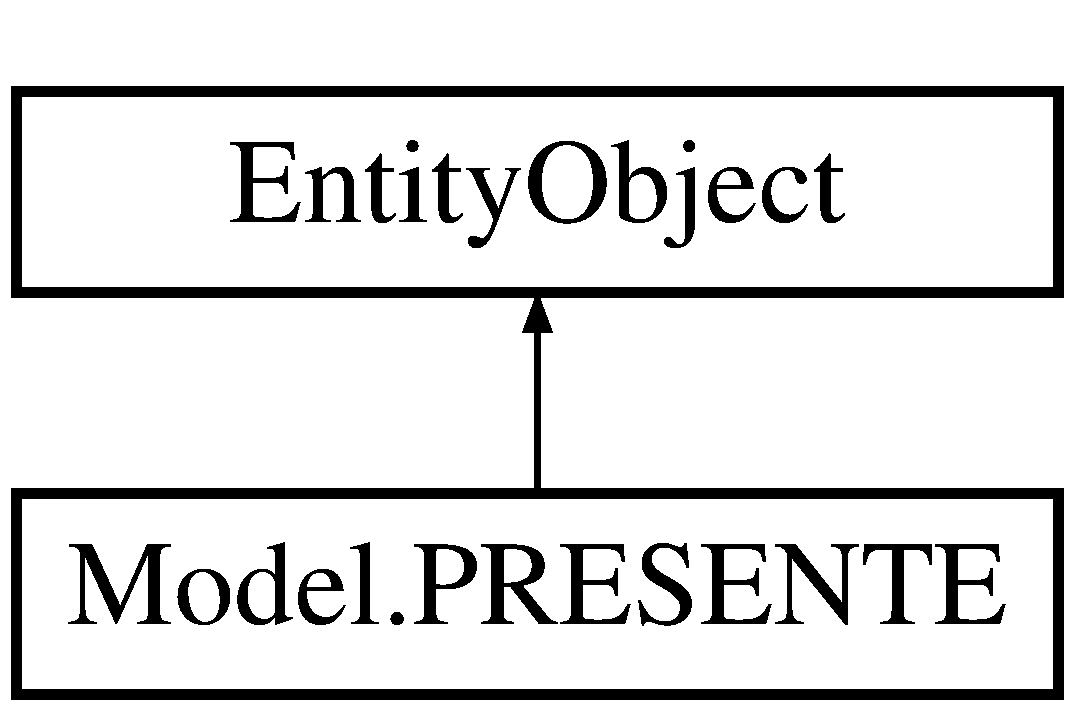
\includegraphics[height=2.000000cm]{class_model_1_1_p_r_e_s_e_n_t_e}
\end{center}
\end{figure}
\subsection*{Static Public Member Functions}
\begin{DoxyCompactItemize}
\item 
static \hyperlink{class_model_1_1_p_r_e_s_e_n_t_e}{P\-R\-E\-S\-E\-N\-T\-E} \hyperlink{class_model_1_1_p_r_e_s_e_n_t_e_a0ef32fb45a1553c8d9fde78dd28d4c36}{Create\-P\-R\-E\-S\-E\-N\-T\-E} (global\-::\-System.\-Int32 \hyperlink{class_model_1_1_p_r_e_s_e_n_t_e_a61ceff1e6daaf303f9bdc311fe3f140e}{num\-\_\-rapport\-\_\-presente}, global\-::\-System.\-String \hyperlink{class_model_1_1_p_r_e_s_e_n_t_e_a182eef0b5545f4d27fb1fbc2838a6bf7}{depot\-\_\-legal\-\_\-presente})
\begin{DoxyCompactList}\small\item\em Créez un nouvel objet \hyperlink{class_model_1_1_p_r_e_s_e_n_t_e}{P\-R\-E\-S\-E\-N\-T\-E}. \end{DoxyCompactList}\end{DoxyCompactItemize}
\subsection*{Properties}
\begin{DoxyCompactItemize}
\item 
Nullable$<$ global\-::\-System.\-Int32 $>$ \hyperlink{class_model_1_1_p_r_e_s_e_n_t_e_afe81dda1e11f4299751d0762ec4b41a7}{quantite\-\_\-presente}\hspace{0.3cm}{\ttfamily  \mbox{[}get, set\mbox{]}}
\begin{DoxyCompactList}\small\item\em Aucune documentation sur les métadonnées n'est disponible. \end{DoxyCompactList}\item 
global\-::\-System.\-Int32 \hyperlink{class_model_1_1_p_r_e_s_e_n_t_e_a61ceff1e6daaf303f9bdc311fe3f140e}{num\-\_\-rapport\-\_\-presente}\hspace{0.3cm}{\ttfamily  \mbox{[}get, set\mbox{]}}
\begin{DoxyCompactList}\small\item\em Aucune documentation sur les métadonnées n'est disponible. \end{DoxyCompactList}\item 
global\-::\-System.\-String \hyperlink{class_model_1_1_p_r_e_s_e_n_t_e_a182eef0b5545f4d27fb1fbc2838a6bf7}{depot\-\_\-legal\-\_\-presente}\hspace{0.3cm}{\ttfamily  \mbox{[}get, set\mbox{]}}
\begin{DoxyCompactList}\small\item\em Aucune documentation sur les métadonnées n'est disponible. \end{DoxyCompactList}\item 
\hyperlink{class_model_1_1_m_e_d_i_c_a_m_e_n_t}{M\-E\-D\-I\-C\-A\-M\-E\-N\-T} \hyperlink{class_model_1_1_p_r_e_s_e_n_t_e_a1ba7b02960d2fcfa2a5ab6f9ad072a0a}{M\-E\-D\-I\-C\-A\-M\-E\-N\-T}\hspace{0.3cm}{\ttfamily  \mbox{[}get, set\mbox{]}}
\begin{DoxyCompactList}\small\item\em Aucune documentation sur les métadonnées n'est disponible. \end{DoxyCompactList}\item 
Entity\-Reference$<$ \hyperlink{class_model_1_1_m_e_d_i_c_a_m_e_n_t}{M\-E\-D\-I\-C\-A\-M\-E\-N\-T} $>$ \hyperlink{class_model_1_1_p_r_e_s_e_n_t_e_aba9cfc5f5f059bd6e19449eb96aadd3a}{M\-E\-D\-I\-C\-A\-M\-E\-N\-T\-Reference}\hspace{0.3cm}{\ttfamily  \mbox{[}get, set\mbox{]}}
\begin{DoxyCompactList}\small\item\em Aucune documentation sur les métadonnées n'est disponible. \end{DoxyCompactList}\item 
\hyperlink{class_model_1_1_r_a_p_p_o_r_t___d_e___v_i_s_i_t_e}{R\-A\-P\-P\-O\-R\-T\-\_\-\-D\-E\-\_\-\-V\-I\-S\-I\-T\-E} \hyperlink{class_model_1_1_p_r_e_s_e_n_t_e_a5a184babcb6553b484a45278f48ce515}{R\-A\-P\-P\-O\-R\-T\-\_\-\-D\-E\-\_\-\-V\-I\-S\-I\-T\-E}\hspace{0.3cm}{\ttfamily  \mbox{[}get, set\mbox{]}}
\begin{DoxyCompactList}\small\item\em Aucune documentation sur les métadonnées n'est disponible. \end{DoxyCompactList}\item 
Entity\-Reference\\*
$<$ \hyperlink{class_model_1_1_r_a_p_p_o_r_t___d_e___v_i_s_i_t_e}{R\-A\-P\-P\-O\-R\-T\-\_\-\-D\-E\-\_\-\-V\-I\-S\-I\-T\-E} $>$ \hyperlink{class_model_1_1_p_r_e_s_e_n_t_e_afa6f45a1ed7ceb1f343ddcdbe55305cb}{R\-A\-P\-P\-O\-R\-T\-\_\-\-D\-E\-\_\-\-V\-I\-S\-I\-T\-E\-Reference}\hspace{0.3cm}{\ttfamily  \mbox{[}get, set\mbox{]}}
\begin{DoxyCompactList}\small\item\em Aucune documentation sur les métadonnées n'est disponible. \end{DoxyCompactList}\end{DoxyCompactItemize}


\subsection{Detailed Description}
Aucune documentation sur les métadonnées n'est disponible. 



\subsection{Member Function Documentation}
\hypertarget{class_model_1_1_p_r_e_s_e_n_t_e_a0ef32fb45a1553c8d9fde78dd28d4c36}{\index{Model\-::\-P\-R\-E\-S\-E\-N\-T\-E@{Model\-::\-P\-R\-E\-S\-E\-N\-T\-E}!Create\-P\-R\-E\-S\-E\-N\-T\-E@{Create\-P\-R\-E\-S\-E\-N\-T\-E}}
\index{Create\-P\-R\-E\-S\-E\-N\-T\-E@{Create\-P\-R\-E\-S\-E\-N\-T\-E}!Model::PRESENTE@{Model\-::\-P\-R\-E\-S\-E\-N\-T\-E}}
\subsubsection[{Create\-P\-R\-E\-S\-E\-N\-T\-E}]{\setlength{\rightskip}{0pt plus 5cm}static {\bf P\-R\-E\-S\-E\-N\-T\-E} Model.\-P\-R\-E\-S\-E\-N\-T\-E.\-Create\-P\-R\-E\-S\-E\-N\-T\-E (
\begin{DoxyParamCaption}
\item[{global\-::\-System.\-Int32}]{num\-\_\-rapport\-\_\-presente, }
\item[{global\-::\-System.\-String}]{depot\-\_\-legal\-\_\-presente}
\end{DoxyParamCaption}
)\hspace{0.3cm}{\ttfamily [static]}}}\label{class_model_1_1_p_r_e_s_e_n_t_e_a0ef32fb45a1553c8d9fde78dd28d4c36}


Créez un nouvel objet \hyperlink{class_model_1_1_p_r_e_s_e_n_t_e}{P\-R\-E\-S\-E\-N\-T\-E}. 


\begin{DoxyParams}{Parameters}
{\em num\-\_\-rapport\-\_\-presente} & Valeur initiale de la propriété num\-\_\-rapport\-\_\-presente.\\
\hline
{\em depot\-\_\-legal\-\_\-presente} & Valeur initiale de la propriété depot\-\_\-legal\-\_\-presente.\\
\hline
\end{DoxyParams}


\subsection{Property Documentation}
\hypertarget{class_model_1_1_p_r_e_s_e_n_t_e_a182eef0b5545f4d27fb1fbc2838a6bf7}{\index{Model\-::\-P\-R\-E\-S\-E\-N\-T\-E@{Model\-::\-P\-R\-E\-S\-E\-N\-T\-E}!depot\-\_\-legal\-\_\-presente@{depot\-\_\-legal\-\_\-presente}}
\index{depot\-\_\-legal\-\_\-presente@{depot\-\_\-legal\-\_\-presente}!Model::PRESENTE@{Model\-::\-P\-R\-E\-S\-E\-N\-T\-E}}
\subsubsection[{depot\-\_\-legal\-\_\-presente}]{\setlength{\rightskip}{0pt plus 5cm}global.\-System.\-String Model.\-P\-R\-E\-S\-E\-N\-T\-E.\-depot\-\_\-legal\-\_\-presente\hspace{0.3cm}{\ttfamily [get]}, {\ttfamily [set]}}}\label{class_model_1_1_p_r_e_s_e_n_t_e_a182eef0b5545f4d27fb1fbc2838a6bf7}


Aucune documentation sur les métadonnées n'est disponible. 

\hypertarget{class_model_1_1_p_r_e_s_e_n_t_e_a1ba7b02960d2fcfa2a5ab6f9ad072a0a}{\index{Model\-::\-P\-R\-E\-S\-E\-N\-T\-E@{Model\-::\-P\-R\-E\-S\-E\-N\-T\-E}!M\-E\-D\-I\-C\-A\-M\-E\-N\-T@{M\-E\-D\-I\-C\-A\-M\-E\-N\-T}}
\index{M\-E\-D\-I\-C\-A\-M\-E\-N\-T@{M\-E\-D\-I\-C\-A\-M\-E\-N\-T}!Model::PRESENTE@{Model\-::\-P\-R\-E\-S\-E\-N\-T\-E}}
\subsubsection[{M\-E\-D\-I\-C\-A\-M\-E\-N\-T}]{\setlength{\rightskip}{0pt plus 5cm}{\bf M\-E\-D\-I\-C\-A\-M\-E\-N\-T} Model.\-P\-R\-E\-S\-E\-N\-T\-E.\-M\-E\-D\-I\-C\-A\-M\-E\-N\-T\hspace{0.3cm}{\ttfamily [get]}, {\ttfamily [set]}}}\label{class_model_1_1_p_r_e_s_e_n_t_e_a1ba7b02960d2fcfa2a5ab6f9ad072a0a}


Aucune documentation sur les métadonnées n'est disponible. 

\hypertarget{class_model_1_1_p_r_e_s_e_n_t_e_aba9cfc5f5f059bd6e19449eb96aadd3a}{\index{Model\-::\-P\-R\-E\-S\-E\-N\-T\-E@{Model\-::\-P\-R\-E\-S\-E\-N\-T\-E}!M\-E\-D\-I\-C\-A\-M\-E\-N\-T\-Reference@{M\-E\-D\-I\-C\-A\-M\-E\-N\-T\-Reference}}
\index{M\-E\-D\-I\-C\-A\-M\-E\-N\-T\-Reference@{M\-E\-D\-I\-C\-A\-M\-E\-N\-T\-Reference}!Model::PRESENTE@{Model\-::\-P\-R\-E\-S\-E\-N\-T\-E}}
\subsubsection[{M\-E\-D\-I\-C\-A\-M\-E\-N\-T\-Reference}]{\setlength{\rightskip}{0pt plus 5cm}Entity\-Reference$<${\bf M\-E\-D\-I\-C\-A\-M\-E\-N\-T}$>$ Model.\-P\-R\-E\-S\-E\-N\-T\-E.\-M\-E\-D\-I\-C\-A\-M\-E\-N\-T\-Reference\hspace{0.3cm}{\ttfamily [get]}, {\ttfamily [set]}}}\label{class_model_1_1_p_r_e_s_e_n_t_e_aba9cfc5f5f059bd6e19449eb96aadd3a}


Aucune documentation sur les métadonnées n'est disponible. 

\hypertarget{class_model_1_1_p_r_e_s_e_n_t_e_a61ceff1e6daaf303f9bdc311fe3f140e}{\index{Model\-::\-P\-R\-E\-S\-E\-N\-T\-E@{Model\-::\-P\-R\-E\-S\-E\-N\-T\-E}!num\-\_\-rapport\-\_\-presente@{num\-\_\-rapport\-\_\-presente}}
\index{num\-\_\-rapport\-\_\-presente@{num\-\_\-rapport\-\_\-presente}!Model::PRESENTE@{Model\-::\-P\-R\-E\-S\-E\-N\-T\-E}}
\subsubsection[{num\-\_\-rapport\-\_\-presente}]{\setlength{\rightskip}{0pt plus 5cm}global.\-System.\-Int32 Model.\-P\-R\-E\-S\-E\-N\-T\-E.\-num\-\_\-rapport\-\_\-presente\hspace{0.3cm}{\ttfamily [get]}, {\ttfamily [set]}}}\label{class_model_1_1_p_r_e_s_e_n_t_e_a61ceff1e6daaf303f9bdc311fe3f140e}


Aucune documentation sur les métadonnées n'est disponible. 

\hypertarget{class_model_1_1_p_r_e_s_e_n_t_e_afe81dda1e11f4299751d0762ec4b41a7}{\index{Model\-::\-P\-R\-E\-S\-E\-N\-T\-E@{Model\-::\-P\-R\-E\-S\-E\-N\-T\-E}!quantite\-\_\-presente@{quantite\-\_\-presente}}
\index{quantite\-\_\-presente@{quantite\-\_\-presente}!Model::PRESENTE@{Model\-::\-P\-R\-E\-S\-E\-N\-T\-E}}
\subsubsection[{quantite\-\_\-presente}]{\setlength{\rightskip}{0pt plus 5cm}Nullable$<$global.\-System.\-Int32$>$ Model.\-P\-R\-E\-S\-E\-N\-T\-E.\-quantite\-\_\-presente\hspace{0.3cm}{\ttfamily [get]}, {\ttfamily [set]}}}\label{class_model_1_1_p_r_e_s_e_n_t_e_afe81dda1e11f4299751d0762ec4b41a7}


Aucune documentation sur les métadonnées n'est disponible. 

\hypertarget{class_model_1_1_p_r_e_s_e_n_t_e_a5a184babcb6553b484a45278f48ce515}{\index{Model\-::\-P\-R\-E\-S\-E\-N\-T\-E@{Model\-::\-P\-R\-E\-S\-E\-N\-T\-E}!R\-A\-P\-P\-O\-R\-T\-\_\-\-D\-E\-\_\-\-V\-I\-S\-I\-T\-E@{R\-A\-P\-P\-O\-R\-T\-\_\-\-D\-E\-\_\-\-V\-I\-S\-I\-T\-E}}
\index{R\-A\-P\-P\-O\-R\-T\-\_\-\-D\-E\-\_\-\-V\-I\-S\-I\-T\-E@{R\-A\-P\-P\-O\-R\-T\-\_\-\-D\-E\-\_\-\-V\-I\-S\-I\-T\-E}!Model::PRESENTE@{Model\-::\-P\-R\-E\-S\-E\-N\-T\-E}}
\subsubsection[{R\-A\-P\-P\-O\-R\-T\-\_\-\-D\-E\-\_\-\-V\-I\-S\-I\-T\-E}]{\setlength{\rightskip}{0pt plus 5cm}{\bf R\-A\-P\-P\-O\-R\-T\-\_\-\-D\-E\-\_\-\-V\-I\-S\-I\-T\-E} Model.\-P\-R\-E\-S\-E\-N\-T\-E.\-R\-A\-P\-P\-O\-R\-T\-\_\-\-D\-E\-\_\-\-V\-I\-S\-I\-T\-E\hspace{0.3cm}{\ttfamily [get]}, {\ttfamily [set]}}}\label{class_model_1_1_p_r_e_s_e_n_t_e_a5a184babcb6553b484a45278f48ce515}


Aucune documentation sur les métadonnées n'est disponible. 

\hypertarget{class_model_1_1_p_r_e_s_e_n_t_e_afa6f45a1ed7ceb1f343ddcdbe55305cb}{\index{Model\-::\-P\-R\-E\-S\-E\-N\-T\-E@{Model\-::\-P\-R\-E\-S\-E\-N\-T\-E}!R\-A\-P\-P\-O\-R\-T\-\_\-\-D\-E\-\_\-\-V\-I\-S\-I\-T\-E\-Reference@{R\-A\-P\-P\-O\-R\-T\-\_\-\-D\-E\-\_\-\-V\-I\-S\-I\-T\-E\-Reference}}
\index{R\-A\-P\-P\-O\-R\-T\-\_\-\-D\-E\-\_\-\-V\-I\-S\-I\-T\-E\-Reference@{R\-A\-P\-P\-O\-R\-T\-\_\-\-D\-E\-\_\-\-V\-I\-S\-I\-T\-E\-Reference}!Model::PRESENTE@{Model\-::\-P\-R\-E\-S\-E\-N\-T\-E}}
\subsubsection[{R\-A\-P\-P\-O\-R\-T\-\_\-\-D\-E\-\_\-\-V\-I\-S\-I\-T\-E\-Reference}]{\setlength{\rightskip}{0pt plus 5cm}Entity\-Reference$<${\bf R\-A\-P\-P\-O\-R\-T\-\_\-\-D\-E\-\_\-\-V\-I\-S\-I\-T\-E}$>$ Model.\-P\-R\-E\-S\-E\-N\-T\-E.\-R\-A\-P\-P\-O\-R\-T\-\_\-\-D\-E\-\_\-\-V\-I\-S\-I\-T\-E\-Reference\hspace{0.3cm}{\ttfamily [get]}, {\ttfamily [set]}}}\label{class_model_1_1_p_r_e_s_e_n_t_e_afa6f45a1ed7ceb1f343ddcdbe55305cb}


Aucune documentation sur les métadonnées n'est disponible. 



The documentation for this class was generated from the following file\-:\begin{DoxyCompactItemize}
\item 
C\-:/\-Users/dju/\-Documents/\-Visual Studio 2012/\-Projects/\-P\-P\-E/\-P\-P\-E3/\-Model/\hyperlink{_model_bdd_sio_8_designer_8cs}{Model\-Bdd\-Sio.\-Designer.\-cs}\end{DoxyCompactItemize}

\hypertarget{class_model_1_1helpers_1_1_rap_helper}{\section{Model.\-helpers.\-Rap\-Helper Class Reference}
\label{class_model_1_1helpers_1_1_rap_helper}\index{Model.\-helpers.\-Rap\-Helper@{Model.\-helpers.\-Rap\-Helper}}
}
\subsection*{Public Member Functions}
\begin{DoxyCompactItemize}
\item 
\hyperlink{class_model_1_1helpers_1_1_rap_helper_a4534ffa1e232f7c2c40bb36d9326f451}{Rap\-Helper} ()
\item 
List$<$ \hyperlink{class_model_1_1_r_a_p_p_o_r_t___d_e___v_i_s_i_t_e}{R\-A\-P\-P\-O\-R\-T\-\_\-\-D\-E\-\_\-\-V\-I\-S\-I\-T\-E} $>$ \hyperlink{class_model_1_1helpers_1_1_rap_helper_a60b5aa74aaccbce4797bb65e7ac9325b}{Get\-List} ()
\item 
void \hyperlink{class_model_1_1helpers_1_1_rap_helper_a4801a3d4577efcee8e53ea48c148890b}{Insert} (\hyperlink{class_model_1_1_r_a_p_p_o_r_t___d_e___v_i_s_i_t_e}{R\-A\-P\-P\-O\-R\-T\-\_\-\-D\-E\-\_\-\-V\-I\-S\-I\-T\-E} rapport)
\item 
void \hyperlink{class_model_1_1helpers_1_1_rap_helper_a729513eb089cee1ad879529564099c5d}{Update} (\hyperlink{class_model_1_1_r_a_p_p_o_r_t___d_e___v_i_s_i_t_e}{R\-A\-P\-P\-O\-R\-T\-\_\-\-D\-E\-\_\-\-V\-I\-S\-I\-T\-E} rapport)
\item 
void \hyperlink{class_model_1_1helpers_1_1_rap_helper_a3f28310fb21724fe13830177b36ce8fa}{Delete} (\hyperlink{class_model_1_1_r_a_p_p_o_r_t___d_e___v_i_s_i_t_e}{R\-A\-P\-P\-O\-R\-T\-\_\-\-D\-E\-\_\-\-V\-I\-S\-I\-T\-E} rapport)
\end{DoxyCompactItemize}
\subsection*{Properties}
\begin{DoxyCompactItemize}
\item 
static \hyperlink{class_model_1_1helpers_1_1_rap_helper}{Rap\-Helper} \hyperlink{class_model_1_1helpers_1_1_rap_helper_a918ff1e5066a1a39e4fa53b891af545f}{Current}\hspace{0.3cm}{\ttfamily  \mbox{[}get\mbox{]}}
\begin{DoxyCompactList}\small\item\em This is a thread-\/safe, lazy singleton. See \href{http://www.yoda.arachsys.com/csharp/singleton.html}{\tt http\-://www.\-yoda.\-arachsys.\-com/csharp/singleton.\-html} for more details about its implementation. \end{DoxyCompactList}\end{DoxyCompactItemize}


\subsection{Constructor \& Destructor Documentation}
\hypertarget{class_model_1_1helpers_1_1_rap_helper_a4534ffa1e232f7c2c40bb36d9326f451}{\index{Model\-::helpers\-::\-Rap\-Helper@{Model\-::helpers\-::\-Rap\-Helper}!Rap\-Helper@{Rap\-Helper}}
\index{Rap\-Helper@{Rap\-Helper}!Model::helpers::RapHelper@{Model\-::helpers\-::\-Rap\-Helper}}
\subsubsection[{Rap\-Helper}]{\setlength{\rightskip}{0pt plus 5cm}Model.\-helpers.\-Rap\-Helper.\-Rap\-Helper (
\begin{DoxyParamCaption}
{}
\end{DoxyParamCaption}
)}}\label{class_model_1_1helpers_1_1_rap_helper_a4534ffa1e232f7c2c40bb36d9326f451}


\subsection{Member Function Documentation}
\hypertarget{class_model_1_1helpers_1_1_rap_helper_a3f28310fb21724fe13830177b36ce8fa}{\index{Model\-::helpers\-::\-Rap\-Helper@{Model\-::helpers\-::\-Rap\-Helper}!Delete@{Delete}}
\index{Delete@{Delete}!Model::helpers::RapHelper@{Model\-::helpers\-::\-Rap\-Helper}}
\subsubsection[{Delete}]{\setlength{\rightskip}{0pt plus 5cm}void Model.\-helpers.\-Rap\-Helper.\-Delete (
\begin{DoxyParamCaption}
\item[{{\bf R\-A\-P\-P\-O\-R\-T\-\_\-\-D\-E\-\_\-\-V\-I\-S\-I\-T\-E}}]{rapport}
\end{DoxyParamCaption}
)}}\label{class_model_1_1helpers_1_1_rap_helper_a3f28310fb21724fe13830177b36ce8fa}
\hypertarget{class_model_1_1helpers_1_1_rap_helper_a60b5aa74aaccbce4797bb65e7ac9325b}{\index{Model\-::helpers\-::\-Rap\-Helper@{Model\-::helpers\-::\-Rap\-Helper}!Get\-List@{Get\-List}}
\index{Get\-List@{Get\-List}!Model::helpers::RapHelper@{Model\-::helpers\-::\-Rap\-Helper}}
\subsubsection[{Get\-List}]{\setlength{\rightskip}{0pt plus 5cm}List$<${\bf R\-A\-P\-P\-O\-R\-T\-\_\-\-D\-E\-\_\-\-V\-I\-S\-I\-T\-E}$>$ Model.\-helpers.\-Rap\-Helper.\-Get\-List (
\begin{DoxyParamCaption}
{}
\end{DoxyParamCaption}
)}}\label{class_model_1_1helpers_1_1_rap_helper_a60b5aa74aaccbce4797bb65e7ac9325b}
\hypertarget{class_model_1_1helpers_1_1_rap_helper_a4801a3d4577efcee8e53ea48c148890b}{\index{Model\-::helpers\-::\-Rap\-Helper@{Model\-::helpers\-::\-Rap\-Helper}!Insert@{Insert}}
\index{Insert@{Insert}!Model::helpers::RapHelper@{Model\-::helpers\-::\-Rap\-Helper}}
\subsubsection[{Insert}]{\setlength{\rightskip}{0pt plus 5cm}void Model.\-helpers.\-Rap\-Helper.\-Insert (
\begin{DoxyParamCaption}
\item[{{\bf R\-A\-P\-P\-O\-R\-T\-\_\-\-D\-E\-\_\-\-V\-I\-S\-I\-T\-E}}]{rapport}
\end{DoxyParamCaption}
)}}\label{class_model_1_1helpers_1_1_rap_helper_a4801a3d4577efcee8e53ea48c148890b}
\hypertarget{class_model_1_1helpers_1_1_rap_helper_a729513eb089cee1ad879529564099c5d}{\index{Model\-::helpers\-::\-Rap\-Helper@{Model\-::helpers\-::\-Rap\-Helper}!Update@{Update}}
\index{Update@{Update}!Model::helpers::RapHelper@{Model\-::helpers\-::\-Rap\-Helper}}
\subsubsection[{Update}]{\setlength{\rightskip}{0pt plus 5cm}void Model.\-helpers.\-Rap\-Helper.\-Update (
\begin{DoxyParamCaption}
\item[{{\bf R\-A\-P\-P\-O\-R\-T\-\_\-\-D\-E\-\_\-\-V\-I\-S\-I\-T\-E}}]{rapport}
\end{DoxyParamCaption}
)}}\label{class_model_1_1helpers_1_1_rap_helper_a729513eb089cee1ad879529564099c5d}


\subsection{Property Documentation}
\hypertarget{class_model_1_1helpers_1_1_rap_helper_a918ff1e5066a1a39e4fa53b891af545f}{\index{Model\-::helpers\-::\-Rap\-Helper@{Model\-::helpers\-::\-Rap\-Helper}!Current@{Current}}
\index{Current@{Current}!Model::helpers::RapHelper@{Model\-::helpers\-::\-Rap\-Helper}}
\subsubsection[{Current}]{\setlength{\rightskip}{0pt plus 5cm}{\bf Rap\-Helper} Model.\-helpers.\-Rap\-Helper.\-Current\hspace{0.3cm}{\ttfamily [static]}, {\ttfamily [get]}}}\label{class_model_1_1helpers_1_1_rap_helper_a918ff1e5066a1a39e4fa53b891af545f}


This is a thread-\/safe, lazy singleton. See \href{http://www.yoda.arachsys.com/csharp/singleton.html}{\tt http\-://www.\-yoda.\-arachsys.\-com/csharp/singleton.\-html} for more details about its implementation. 



The documentation for this class was generated from the following file\-:\begin{DoxyCompactItemize}
\item 
C\-:/\-Users/dju/\-Documents/\-Visual Studio 2012/\-Projects/\-P\-P\-E/\-P\-P\-E3/\-Model/helpers/\hyperlink{_rap_helper_8cs}{Rap\-Helper.\-cs}\end{DoxyCompactItemize}

\hypertarget{class_model_1_1_r_a_p_p_o_r_t___d_e___v_i_s_i_t_e}{\section{Model.\-R\-A\-P\-P\-O\-R\-T\-\_\-\-D\-E\-\_\-\-V\-I\-S\-I\-T\-E Class Reference}
\label{class_model_1_1_r_a_p_p_o_r_t___d_e___v_i_s_i_t_e}\index{Model.\-R\-A\-P\-P\-O\-R\-T\-\_\-\-D\-E\-\_\-\-V\-I\-S\-I\-T\-E@{Model.\-R\-A\-P\-P\-O\-R\-T\-\_\-\-D\-E\-\_\-\-V\-I\-S\-I\-T\-E}}
}


Aucune documentation sur les métadonnées n'est disponible.  


Inheritance diagram for Model.\-R\-A\-P\-P\-O\-R\-T\-\_\-\-D\-E\-\_\-\-V\-I\-S\-I\-T\-E\-:\begin{figure}[H]
\begin{center}
\leavevmode
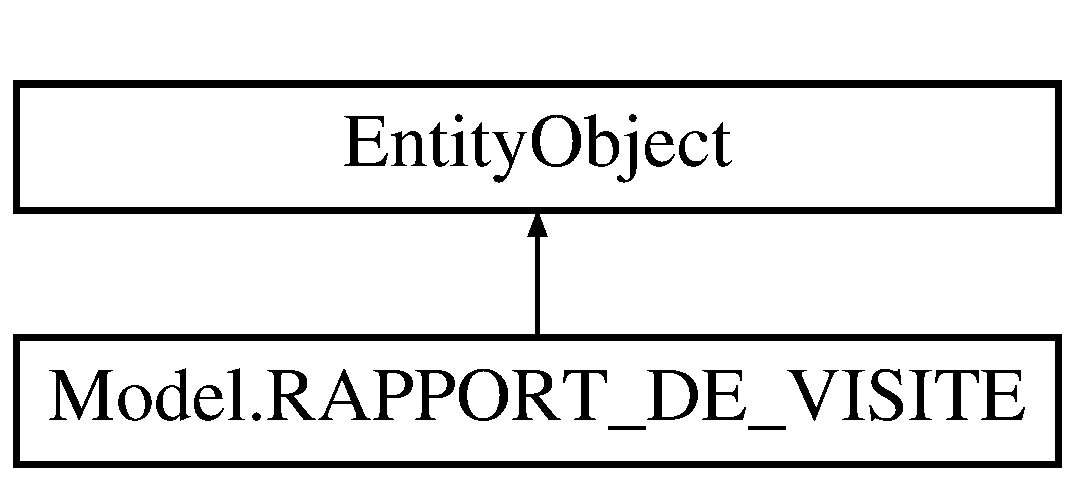
\includegraphics[height=2.000000cm]{class_model_1_1_r_a_p_p_o_r_t___d_e___v_i_s_i_t_e}
\end{center}
\end{figure}
\subsection*{Static Public Member Functions}
\begin{DoxyCompactItemize}
\item 
static \hyperlink{class_model_1_1_r_a_p_p_o_r_t___d_e___v_i_s_i_t_e}{R\-A\-P\-P\-O\-R\-T\-\_\-\-D\-E\-\_\-\-V\-I\-S\-I\-T\-E} \hyperlink{class_model_1_1_r_a_p_p_o_r_t___d_e___v_i_s_i_t_e_afa4d9449adaeca7892e1ac70f28dcd04}{Create\-R\-A\-P\-P\-O\-R\-T\-\_\-\-D\-E\-\_\-\-V\-I\-S\-I\-T\-E} (global\-::\-System.\-Int32 \hyperlink{class_model_1_1_r_a_p_p_o_r_t___d_e___v_i_s_i_t_e_a09579a805a9a16ca3d590de786e1f2ff}{num\-\_\-rapport}, global\-::\-System.\-Date\-Time \hyperlink{class_model_1_1_r_a_p_p_o_r_t___d_e___v_i_s_i_t_e_a0158656f483091006f9c9a9ba5faa9ad}{date\-\_\-rapport}, global\-::\-System.\-Date\-Time \hyperlink{class_model_1_1_r_a_p_p_o_r_t___d_e___v_i_s_i_t_e_a3ededfc7a2aa19b96cb389900c2e6e36}{date\-\_\-visite}, global\-::\-System.\-String \hyperlink{class_model_1_1_r_a_p_p_o_r_t___d_e___v_i_s_i_t_e_a916f42e4c755e24452e9037997dfbb35}{bilan\-\_\-visite})
\begin{DoxyCompactList}\small\item\em Créez un nouvel objet \hyperlink{class_model_1_1_r_a_p_p_o_r_t___d_e___v_i_s_i_t_e}{R\-A\-P\-P\-O\-R\-T\-\_\-\-D\-E\-\_\-\-V\-I\-S\-I\-T\-E}. \end{DoxyCompactList}\end{DoxyCompactItemize}
\subsection*{Properties}
\begin{DoxyCompactItemize}
\item 
global\-::\-System.\-Int32 \hyperlink{class_model_1_1_r_a_p_p_o_r_t___d_e___v_i_s_i_t_e_a09579a805a9a16ca3d590de786e1f2ff}{num\-\_\-rapport}\hspace{0.3cm}{\ttfamily  \mbox{[}get, set\mbox{]}}
\begin{DoxyCompactList}\small\item\em Aucune documentation sur les métadonnées n'est disponible. \end{DoxyCompactList}\item 
Nullable$<$ global\-::\-System.\-Int32 $>$ \hyperlink{class_model_1_1_r_a_p_p_o_r_t___d_e___v_i_s_i_t_e_a57873cda816b38fbd05d2e659fb45c35}{code\-\_\-motif}\hspace{0.3cm}{\ttfamily  \mbox{[}get, set\mbox{]}}
\begin{DoxyCompactList}\small\item\em Aucune documentation sur les métadonnées n'est disponible. \end{DoxyCompactList}\item 
Nullable$<$ global\-::\-System.\-Int32 $>$ \hyperlink{class_model_1_1_r_a_p_p_o_r_t___d_e___v_i_s_i_t_e_a8afd6d68f9e91bc0eef72f0d6f1d9576}{matricule\-\_\-praticien}\hspace{0.3cm}{\ttfamily  \mbox{[}get, set\mbox{]}}
\begin{DoxyCompactList}\small\item\em Aucune documentation sur les métadonnées n'est disponible. \end{DoxyCompactList}\item 
global\-::\-System.\-Date\-Time \hyperlink{class_model_1_1_r_a_p_p_o_r_t___d_e___v_i_s_i_t_e_a0158656f483091006f9c9a9ba5faa9ad}{date\-\_\-rapport}\hspace{0.3cm}{\ttfamily  \mbox{[}get, set\mbox{]}}
\begin{DoxyCompactList}\small\item\em Aucune documentation sur les métadonnées n'est disponible. \end{DoxyCompactList}\item 
global\-::\-System.\-Date\-Time \hyperlink{class_model_1_1_r_a_p_p_o_r_t___d_e___v_i_s_i_t_e_a3ededfc7a2aa19b96cb389900c2e6e36}{date\-\_\-visite}\hspace{0.3cm}{\ttfamily  \mbox{[}get, set\mbox{]}}
\begin{DoxyCompactList}\small\item\em Aucune documentation sur les métadonnées n'est disponible. \end{DoxyCompactList}\item 
global\-::\-System.\-String \hyperlink{class_model_1_1_r_a_p_p_o_r_t___d_e___v_i_s_i_t_e_a916f42e4c755e24452e9037997dfbb35}{bilan\-\_\-visite}\hspace{0.3cm}{\ttfamily  \mbox{[}get, set\mbox{]}}
\begin{DoxyCompactList}\small\item\em Aucune documentation sur les métadonnées n'est disponible. \end{DoxyCompactList}\item 
Nullable$<$ global\-::\-System.\-Int32 $>$ \hyperlink{class_model_1_1_r_a_p_p_o_r_t___d_e___v_i_s_i_t_e_aad653ab33335adde420671e5af84cbce}{matricule\-\_\-col}\hspace{0.3cm}{\ttfamily  \mbox{[}get, set\mbox{]}}
\begin{DoxyCompactList}\small\item\em Aucune documentation sur les métadonnées n'est disponible. \end{DoxyCompactList}\item 
\hyperlink{class_model_1_1_m_o_t_i_f}{M\-O\-T\-I\-F} \hyperlink{class_model_1_1_r_a_p_p_o_r_t___d_e___v_i_s_i_t_e_abb54ed863ff048a69698fcf9e4b7665c}{M\-O\-T\-I\-F}\hspace{0.3cm}{\ttfamily  \mbox{[}get, set\mbox{]}}
\begin{DoxyCompactList}\small\item\em Aucune documentation sur les métadonnées n'est disponible. \end{DoxyCompactList}\item 
Entity\-Reference$<$ \hyperlink{class_model_1_1_m_o_t_i_f}{M\-O\-T\-I\-F} $>$ \hyperlink{class_model_1_1_r_a_p_p_o_r_t___d_e___v_i_s_i_t_e_addf9ad62b216faa0ee68ff497faac083}{M\-O\-T\-I\-F\-Reference}\hspace{0.3cm}{\ttfamily  \mbox{[}get, set\mbox{]}}
\begin{DoxyCompactList}\small\item\em Aucune documentation sur les métadonnées n'est disponible. \end{DoxyCompactList}\item 
\hyperlink{class_model_1_1_p_r_a_t_i_c_i_e_n}{P\-R\-A\-T\-I\-C\-I\-E\-N} \hyperlink{class_model_1_1_r_a_p_p_o_r_t___d_e___v_i_s_i_t_e_ac30bad0961e26f2899f13d860c4d5f65}{P\-R\-A\-T\-I\-C\-I\-E\-N}\hspace{0.3cm}{\ttfamily  \mbox{[}get, set\mbox{]}}
\begin{DoxyCompactList}\small\item\em Aucune documentation sur les métadonnées n'est disponible. \end{DoxyCompactList}\item 
Entity\-Reference$<$ \hyperlink{class_model_1_1_p_r_a_t_i_c_i_e_n}{P\-R\-A\-T\-I\-C\-I\-E\-N} $>$ \hyperlink{class_model_1_1_r_a_p_p_o_r_t___d_e___v_i_s_i_t_e_a54eeb4d8f7c4a50370f1803ba841a36a}{P\-R\-A\-T\-I\-C\-I\-E\-N\-Reference}\hspace{0.3cm}{\ttfamily  \mbox{[}get, set\mbox{]}}
\begin{DoxyCompactList}\small\item\em Aucune documentation sur les métadonnées n'est disponible. \end{DoxyCompactList}\item 
\hyperlink{class_model_1_1_c_o_l_l_a_b_o_r_a_t_e_u_r}{C\-O\-L\-L\-A\-B\-O\-R\-A\-T\-E\-U\-R} \hyperlink{class_model_1_1_r_a_p_p_o_r_t___d_e___v_i_s_i_t_e_ae2e3abe90339d6fbacb2990f382c9380}{C\-O\-L\-L\-A\-B\-O\-R\-A\-T\-E\-U\-R}\hspace{0.3cm}{\ttfamily  \mbox{[}get, set\mbox{]}}
\begin{DoxyCompactList}\small\item\em Aucune documentation sur les métadonnées n'est disponible. \end{DoxyCompactList}\item 
Entity\-Reference$<$ \hyperlink{class_model_1_1_c_o_l_l_a_b_o_r_a_t_e_u_r}{C\-O\-L\-L\-A\-B\-O\-R\-A\-T\-E\-U\-R} $>$ \hyperlink{class_model_1_1_r_a_p_p_o_r_t___d_e___v_i_s_i_t_e_a14d1d3b1a7760c1c07bd940a84cb3a32}{C\-O\-L\-L\-A\-B\-O\-R\-A\-T\-E\-U\-R\-Reference}\hspace{0.3cm}{\ttfamily  \mbox{[}get, set\mbox{]}}
\begin{DoxyCompactList}\small\item\em Aucune documentation sur les métadonnées n'est disponible. \end{DoxyCompactList}\item 
Entity\-Collection$<$ \hyperlink{class_model_1_1_o_f_f_r_e1}{O\-F\-F\-R\-E1} $>$ \hyperlink{class_model_1_1_r_a_p_p_o_r_t___d_e___v_i_s_i_t_e_a366487e6a939936711605d454b16a332}{O\-F\-F\-R\-E}\hspace{0.3cm}{\ttfamily  \mbox{[}get, set\mbox{]}}
\begin{DoxyCompactList}\small\item\em Aucune documentation sur les métadonnées n'est disponible. \end{DoxyCompactList}\item 
Entity\-Collection$<$ \hyperlink{class_model_1_1_p_r_e_s_e_n_t_e}{P\-R\-E\-S\-E\-N\-T\-E} $>$ \hyperlink{class_model_1_1_r_a_p_p_o_r_t___d_e___v_i_s_i_t_e_a78d24aba4a7730f7dcd96bc508376855}{P\-R\-E\-S\-E\-N\-T\-E}\hspace{0.3cm}{\ttfamily  \mbox{[}get, set\mbox{]}}
\begin{DoxyCompactList}\small\item\em Aucune documentation sur les métadonnées n'est disponible. \end{DoxyCompactList}\end{DoxyCompactItemize}


\subsection{Detailed Description}
Aucune documentation sur les métadonnées n'est disponible. 



\subsection{Member Function Documentation}
\hypertarget{class_model_1_1_r_a_p_p_o_r_t___d_e___v_i_s_i_t_e_afa4d9449adaeca7892e1ac70f28dcd04}{\index{Model\-::\-R\-A\-P\-P\-O\-R\-T\-\_\-\-D\-E\-\_\-\-V\-I\-S\-I\-T\-E@{Model\-::\-R\-A\-P\-P\-O\-R\-T\-\_\-\-D\-E\-\_\-\-V\-I\-S\-I\-T\-E}!Create\-R\-A\-P\-P\-O\-R\-T\-\_\-\-D\-E\-\_\-\-V\-I\-S\-I\-T\-E@{Create\-R\-A\-P\-P\-O\-R\-T\-\_\-\-D\-E\-\_\-\-V\-I\-S\-I\-T\-E}}
\index{Create\-R\-A\-P\-P\-O\-R\-T\-\_\-\-D\-E\-\_\-\-V\-I\-S\-I\-T\-E@{Create\-R\-A\-P\-P\-O\-R\-T\-\_\-\-D\-E\-\_\-\-V\-I\-S\-I\-T\-E}!Model::RAPPORT_DE_VISITE@{Model\-::\-R\-A\-P\-P\-O\-R\-T\-\_\-\-D\-E\-\_\-\-V\-I\-S\-I\-T\-E}}
\subsubsection[{Create\-R\-A\-P\-P\-O\-R\-T\-\_\-\-D\-E\-\_\-\-V\-I\-S\-I\-T\-E}]{\setlength{\rightskip}{0pt plus 5cm}static {\bf R\-A\-P\-P\-O\-R\-T\-\_\-\-D\-E\-\_\-\-V\-I\-S\-I\-T\-E} Model.\-R\-A\-P\-P\-O\-R\-T\-\_\-\-D\-E\-\_\-\-V\-I\-S\-I\-T\-E.\-Create\-R\-A\-P\-P\-O\-R\-T\-\_\-\-D\-E\-\_\-\-V\-I\-S\-I\-T\-E (
\begin{DoxyParamCaption}
\item[{global\-::\-System.\-Int32}]{num\-\_\-rapport, }
\item[{global\-::\-System.\-Date\-Time}]{date\-\_\-rapport, }
\item[{global\-::\-System.\-Date\-Time}]{date\-\_\-visite, }
\item[{global\-::\-System.\-String}]{bilan\-\_\-visite}
\end{DoxyParamCaption}
)\hspace{0.3cm}{\ttfamily [static]}}}\label{class_model_1_1_r_a_p_p_o_r_t___d_e___v_i_s_i_t_e_afa4d9449adaeca7892e1ac70f28dcd04}


Créez un nouvel objet \hyperlink{class_model_1_1_r_a_p_p_o_r_t___d_e___v_i_s_i_t_e}{R\-A\-P\-P\-O\-R\-T\-\_\-\-D\-E\-\_\-\-V\-I\-S\-I\-T\-E}. 


\begin{DoxyParams}{Parameters}
{\em num\-\_\-rapport} & Valeur initiale de la propriété num\-\_\-rapport.\\
\hline
{\em date\-\_\-rapport} & Valeur initiale de la propriété date\-\_\-rapport.\\
\hline
{\em date\-\_\-visite} & Valeur initiale de la propriété date\-\_\-visite.\\
\hline
{\em bilan\-\_\-visite} & Valeur initiale de la propriété bilan\-\_\-visite.\\
\hline
\end{DoxyParams}


\subsection{Property Documentation}
\hypertarget{class_model_1_1_r_a_p_p_o_r_t___d_e___v_i_s_i_t_e_a916f42e4c755e24452e9037997dfbb35}{\index{Model\-::\-R\-A\-P\-P\-O\-R\-T\-\_\-\-D\-E\-\_\-\-V\-I\-S\-I\-T\-E@{Model\-::\-R\-A\-P\-P\-O\-R\-T\-\_\-\-D\-E\-\_\-\-V\-I\-S\-I\-T\-E}!bilan\-\_\-visite@{bilan\-\_\-visite}}
\index{bilan\-\_\-visite@{bilan\-\_\-visite}!Model::RAPPORT_DE_VISITE@{Model\-::\-R\-A\-P\-P\-O\-R\-T\-\_\-\-D\-E\-\_\-\-V\-I\-S\-I\-T\-E}}
\subsubsection[{bilan\-\_\-visite}]{\setlength{\rightskip}{0pt plus 5cm}global.\-System.\-String Model.\-R\-A\-P\-P\-O\-R\-T\-\_\-\-D\-E\-\_\-\-V\-I\-S\-I\-T\-E.\-bilan\-\_\-visite\hspace{0.3cm}{\ttfamily [get]}, {\ttfamily [set]}}}\label{class_model_1_1_r_a_p_p_o_r_t___d_e___v_i_s_i_t_e_a916f42e4c755e24452e9037997dfbb35}


Aucune documentation sur les métadonnées n'est disponible. 

\hypertarget{class_model_1_1_r_a_p_p_o_r_t___d_e___v_i_s_i_t_e_a57873cda816b38fbd05d2e659fb45c35}{\index{Model\-::\-R\-A\-P\-P\-O\-R\-T\-\_\-\-D\-E\-\_\-\-V\-I\-S\-I\-T\-E@{Model\-::\-R\-A\-P\-P\-O\-R\-T\-\_\-\-D\-E\-\_\-\-V\-I\-S\-I\-T\-E}!code\-\_\-motif@{code\-\_\-motif}}
\index{code\-\_\-motif@{code\-\_\-motif}!Model::RAPPORT_DE_VISITE@{Model\-::\-R\-A\-P\-P\-O\-R\-T\-\_\-\-D\-E\-\_\-\-V\-I\-S\-I\-T\-E}}
\subsubsection[{code\-\_\-motif}]{\setlength{\rightskip}{0pt plus 5cm}Nullable$<$global.\-System.\-Int32$>$ Model.\-R\-A\-P\-P\-O\-R\-T\-\_\-\-D\-E\-\_\-\-V\-I\-S\-I\-T\-E.\-code\-\_\-motif\hspace{0.3cm}{\ttfamily [get]}, {\ttfamily [set]}}}\label{class_model_1_1_r_a_p_p_o_r_t___d_e___v_i_s_i_t_e_a57873cda816b38fbd05d2e659fb45c35}


Aucune documentation sur les métadonnées n'est disponible. 

\hypertarget{class_model_1_1_r_a_p_p_o_r_t___d_e___v_i_s_i_t_e_ae2e3abe90339d6fbacb2990f382c9380}{\index{Model\-::\-R\-A\-P\-P\-O\-R\-T\-\_\-\-D\-E\-\_\-\-V\-I\-S\-I\-T\-E@{Model\-::\-R\-A\-P\-P\-O\-R\-T\-\_\-\-D\-E\-\_\-\-V\-I\-S\-I\-T\-E}!C\-O\-L\-L\-A\-B\-O\-R\-A\-T\-E\-U\-R@{C\-O\-L\-L\-A\-B\-O\-R\-A\-T\-E\-U\-R}}
\index{C\-O\-L\-L\-A\-B\-O\-R\-A\-T\-E\-U\-R@{C\-O\-L\-L\-A\-B\-O\-R\-A\-T\-E\-U\-R}!Model::RAPPORT_DE_VISITE@{Model\-::\-R\-A\-P\-P\-O\-R\-T\-\_\-\-D\-E\-\_\-\-V\-I\-S\-I\-T\-E}}
\subsubsection[{C\-O\-L\-L\-A\-B\-O\-R\-A\-T\-E\-U\-R}]{\setlength{\rightskip}{0pt plus 5cm}{\bf C\-O\-L\-L\-A\-B\-O\-R\-A\-T\-E\-U\-R} Model.\-R\-A\-P\-P\-O\-R\-T\-\_\-\-D\-E\-\_\-\-V\-I\-S\-I\-T\-E.\-C\-O\-L\-L\-A\-B\-O\-R\-A\-T\-E\-U\-R\hspace{0.3cm}{\ttfamily [get]}, {\ttfamily [set]}}}\label{class_model_1_1_r_a_p_p_o_r_t___d_e___v_i_s_i_t_e_ae2e3abe90339d6fbacb2990f382c9380}


Aucune documentation sur les métadonnées n'est disponible. 

\hypertarget{class_model_1_1_r_a_p_p_o_r_t___d_e___v_i_s_i_t_e_a14d1d3b1a7760c1c07bd940a84cb3a32}{\index{Model\-::\-R\-A\-P\-P\-O\-R\-T\-\_\-\-D\-E\-\_\-\-V\-I\-S\-I\-T\-E@{Model\-::\-R\-A\-P\-P\-O\-R\-T\-\_\-\-D\-E\-\_\-\-V\-I\-S\-I\-T\-E}!C\-O\-L\-L\-A\-B\-O\-R\-A\-T\-E\-U\-R\-Reference@{C\-O\-L\-L\-A\-B\-O\-R\-A\-T\-E\-U\-R\-Reference}}
\index{C\-O\-L\-L\-A\-B\-O\-R\-A\-T\-E\-U\-R\-Reference@{C\-O\-L\-L\-A\-B\-O\-R\-A\-T\-E\-U\-R\-Reference}!Model::RAPPORT_DE_VISITE@{Model\-::\-R\-A\-P\-P\-O\-R\-T\-\_\-\-D\-E\-\_\-\-V\-I\-S\-I\-T\-E}}
\subsubsection[{C\-O\-L\-L\-A\-B\-O\-R\-A\-T\-E\-U\-R\-Reference}]{\setlength{\rightskip}{0pt plus 5cm}Entity\-Reference$<${\bf C\-O\-L\-L\-A\-B\-O\-R\-A\-T\-E\-U\-R}$>$ Model.\-R\-A\-P\-P\-O\-R\-T\-\_\-\-D\-E\-\_\-\-V\-I\-S\-I\-T\-E.\-C\-O\-L\-L\-A\-B\-O\-R\-A\-T\-E\-U\-R\-Reference\hspace{0.3cm}{\ttfamily [get]}, {\ttfamily [set]}}}\label{class_model_1_1_r_a_p_p_o_r_t___d_e___v_i_s_i_t_e_a14d1d3b1a7760c1c07bd940a84cb3a32}


Aucune documentation sur les métadonnées n'est disponible. 

\hypertarget{class_model_1_1_r_a_p_p_o_r_t___d_e___v_i_s_i_t_e_a0158656f483091006f9c9a9ba5faa9ad}{\index{Model\-::\-R\-A\-P\-P\-O\-R\-T\-\_\-\-D\-E\-\_\-\-V\-I\-S\-I\-T\-E@{Model\-::\-R\-A\-P\-P\-O\-R\-T\-\_\-\-D\-E\-\_\-\-V\-I\-S\-I\-T\-E}!date\-\_\-rapport@{date\-\_\-rapport}}
\index{date\-\_\-rapport@{date\-\_\-rapport}!Model::RAPPORT_DE_VISITE@{Model\-::\-R\-A\-P\-P\-O\-R\-T\-\_\-\-D\-E\-\_\-\-V\-I\-S\-I\-T\-E}}
\subsubsection[{date\-\_\-rapport}]{\setlength{\rightskip}{0pt plus 5cm}global.\-System.\-Date\-Time Model.\-R\-A\-P\-P\-O\-R\-T\-\_\-\-D\-E\-\_\-\-V\-I\-S\-I\-T\-E.\-date\-\_\-rapport\hspace{0.3cm}{\ttfamily [get]}, {\ttfamily [set]}}}\label{class_model_1_1_r_a_p_p_o_r_t___d_e___v_i_s_i_t_e_a0158656f483091006f9c9a9ba5faa9ad}


Aucune documentation sur les métadonnées n'est disponible. 

\hypertarget{class_model_1_1_r_a_p_p_o_r_t___d_e___v_i_s_i_t_e_a3ededfc7a2aa19b96cb389900c2e6e36}{\index{Model\-::\-R\-A\-P\-P\-O\-R\-T\-\_\-\-D\-E\-\_\-\-V\-I\-S\-I\-T\-E@{Model\-::\-R\-A\-P\-P\-O\-R\-T\-\_\-\-D\-E\-\_\-\-V\-I\-S\-I\-T\-E}!date\-\_\-visite@{date\-\_\-visite}}
\index{date\-\_\-visite@{date\-\_\-visite}!Model::RAPPORT_DE_VISITE@{Model\-::\-R\-A\-P\-P\-O\-R\-T\-\_\-\-D\-E\-\_\-\-V\-I\-S\-I\-T\-E}}
\subsubsection[{date\-\_\-visite}]{\setlength{\rightskip}{0pt plus 5cm}global.\-System.\-Date\-Time Model.\-R\-A\-P\-P\-O\-R\-T\-\_\-\-D\-E\-\_\-\-V\-I\-S\-I\-T\-E.\-date\-\_\-visite\hspace{0.3cm}{\ttfamily [get]}, {\ttfamily [set]}}}\label{class_model_1_1_r_a_p_p_o_r_t___d_e___v_i_s_i_t_e_a3ededfc7a2aa19b96cb389900c2e6e36}


Aucune documentation sur les métadonnées n'est disponible. 

\hypertarget{class_model_1_1_r_a_p_p_o_r_t___d_e___v_i_s_i_t_e_aad653ab33335adde420671e5af84cbce}{\index{Model\-::\-R\-A\-P\-P\-O\-R\-T\-\_\-\-D\-E\-\_\-\-V\-I\-S\-I\-T\-E@{Model\-::\-R\-A\-P\-P\-O\-R\-T\-\_\-\-D\-E\-\_\-\-V\-I\-S\-I\-T\-E}!matricule\-\_\-col@{matricule\-\_\-col}}
\index{matricule\-\_\-col@{matricule\-\_\-col}!Model::RAPPORT_DE_VISITE@{Model\-::\-R\-A\-P\-P\-O\-R\-T\-\_\-\-D\-E\-\_\-\-V\-I\-S\-I\-T\-E}}
\subsubsection[{matricule\-\_\-col}]{\setlength{\rightskip}{0pt plus 5cm}Nullable$<$global.\-System.\-Int32$>$ Model.\-R\-A\-P\-P\-O\-R\-T\-\_\-\-D\-E\-\_\-\-V\-I\-S\-I\-T\-E.\-matricule\-\_\-col\hspace{0.3cm}{\ttfamily [get]}, {\ttfamily [set]}}}\label{class_model_1_1_r_a_p_p_o_r_t___d_e___v_i_s_i_t_e_aad653ab33335adde420671e5af84cbce}


Aucune documentation sur les métadonnées n'est disponible. 

\hypertarget{class_model_1_1_r_a_p_p_o_r_t___d_e___v_i_s_i_t_e_a8afd6d68f9e91bc0eef72f0d6f1d9576}{\index{Model\-::\-R\-A\-P\-P\-O\-R\-T\-\_\-\-D\-E\-\_\-\-V\-I\-S\-I\-T\-E@{Model\-::\-R\-A\-P\-P\-O\-R\-T\-\_\-\-D\-E\-\_\-\-V\-I\-S\-I\-T\-E}!matricule\-\_\-praticien@{matricule\-\_\-praticien}}
\index{matricule\-\_\-praticien@{matricule\-\_\-praticien}!Model::RAPPORT_DE_VISITE@{Model\-::\-R\-A\-P\-P\-O\-R\-T\-\_\-\-D\-E\-\_\-\-V\-I\-S\-I\-T\-E}}
\subsubsection[{matricule\-\_\-praticien}]{\setlength{\rightskip}{0pt plus 5cm}Nullable$<$global.\-System.\-Int32$>$ Model.\-R\-A\-P\-P\-O\-R\-T\-\_\-\-D\-E\-\_\-\-V\-I\-S\-I\-T\-E.\-matricule\-\_\-praticien\hspace{0.3cm}{\ttfamily [get]}, {\ttfamily [set]}}}\label{class_model_1_1_r_a_p_p_o_r_t___d_e___v_i_s_i_t_e_a8afd6d68f9e91bc0eef72f0d6f1d9576}


Aucune documentation sur les métadonnées n'est disponible. 

\hypertarget{class_model_1_1_r_a_p_p_o_r_t___d_e___v_i_s_i_t_e_abb54ed863ff048a69698fcf9e4b7665c}{\index{Model\-::\-R\-A\-P\-P\-O\-R\-T\-\_\-\-D\-E\-\_\-\-V\-I\-S\-I\-T\-E@{Model\-::\-R\-A\-P\-P\-O\-R\-T\-\_\-\-D\-E\-\_\-\-V\-I\-S\-I\-T\-E}!M\-O\-T\-I\-F@{M\-O\-T\-I\-F}}
\index{M\-O\-T\-I\-F@{M\-O\-T\-I\-F}!Model::RAPPORT_DE_VISITE@{Model\-::\-R\-A\-P\-P\-O\-R\-T\-\_\-\-D\-E\-\_\-\-V\-I\-S\-I\-T\-E}}
\subsubsection[{M\-O\-T\-I\-F}]{\setlength{\rightskip}{0pt plus 5cm}{\bf M\-O\-T\-I\-F} Model.\-R\-A\-P\-P\-O\-R\-T\-\_\-\-D\-E\-\_\-\-V\-I\-S\-I\-T\-E.\-M\-O\-T\-I\-F\hspace{0.3cm}{\ttfamily [get]}, {\ttfamily [set]}}}\label{class_model_1_1_r_a_p_p_o_r_t___d_e___v_i_s_i_t_e_abb54ed863ff048a69698fcf9e4b7665c}


Aucune documentation sur les métadonnées n'est disponible. 

\hypertarget{class_model_1_1_r_a_p_p_o_r_t___d_e___v_i_s_i_t_e_addf9ad62b216faa0ee68ff497faac083}{\index{Model\-::\-R\-A\-P\-P\-O\-R\-T\-\_\-\-D\-E\-\_\-\-V\-I\-S\-I\-T\-E@{Model\-::\-R\-A\-P\-P\-O\-R\-T\-\_\-\-D\-E\-\_\-\-V\-I\-S\-I\-T\-E}!M\-O\-T\-I\-F\-Reference@{M\-O\-T\-I\-F\-Reference}}
\index{M\-O\-T\-I\-F\-Reference@{M\-O\-T\-I\-F\-Reference}!Model::RAPPORT_DE_VISITE@{Model\-::\-R\-A\-P\-P\-O\-R\-T\-\_\-\-D\-E\-\_\-\-V\-I\-S\-I\-T\-E}}
\subsubsection[{M\-O\-T\-I\-F\-Reference}]{\setlength{\rightskip}{0pt plus 5cm}Entity\-Reference$<${\bf M\-O\-T\-I\-F}$>$ Model.\-R\-A\-P\-P\-O\-R\-T\-\_\-\-D\-E\-\_\-\-V\-I\-S\-I\-T\-E.\-M\-O\-T\-I\-F\-Reference\hspace{0.3cm}{\ttfamily [get]}, {\ttfamily [set]}}}\label{class_model_1_1_r_a_p_p_o_r_t___d_e___v_i_s_i_t_e_addf9ad62b216faa0ee68ff497faac083}


Aucune documentation sur les métadonnées n'est disponible. 

\hypertarget{class_model_1_1_r_a_p_p_o_r_t___d_e___v_i_s_i_t_e_a09579a805a9a16ca3d590de786e1f2ff}{\index{Model\-::\-R\-A\-P\-P\-O\-R\-T\-\_\-\-D\-E\-\_\-\-V\-I\-S\-I\-T\-E@{Model\-::\-R\-A\-P\-P\-O\-R\-T\-\_\-\-D\-E\-\_\-\-V\-I\-S\-I\-T\-E}!num\-\_\-rapport@{num\-\_\-rapport}}
\index{num\-\_\-rapport@{num\-\_\-rapport}!Model::RAPPORT_DE_VISITE@{Model\-::\-R\-A\-P\-P\-O\-R\-T\-\_\-\-D\-E\-\_\-\-V\-I\-S\-I\-T\-E}}
\subsubsection[{num\-\_\-rapport}]{\setlength{\rightskip}{0pt plus 5cm}global.\-System.\-Int32 Model.\-R\-A\-P\-P\-O\-R\-T\-\_\-\-D\-E\-\_\-\-V\-I\-S\-I\-T\-E.\-num\-\_\-rapport\hspace{0.3cm}{\ttfamily [get]}, {\ttfamily [set]}}}\label{class_model_1_1_r_a_p_p_o_r_t___d_e___v_i_s_i_t_e_a09579a805a9a16ca3d590de786e1f2ff}


Aucune documentation sur les métadonnées n'est disponible. 

\hypertarget{class_model_1_1_r_a_p_p_o_r_t___d_e___v_i_s_i_t_e_a366487e6a939936711605d454b16a332}{\index{Model\-::\-R\-A\-P\-P\-O\-R\-T\-\_\-\-D\-E\-\_\-\-V\-I\-S\-I\-T\-E@{Model\-::\-R\-A\-P\-P\-O\-R\-T\-\_\-\-D\-E\-\_\-\-V\-I\-S\-I\-T\-E}!O\-F\-F\-R\-E@{O\-F\-F\-R\-E}}
\index{O\-F\-F\-R\-E@{O\-F\-F\-R\-E}!Model::RAPPORT_DE_VISITE@{Model\-::\-R\-A\-P\-P\-O\-R\-T\-\_\-\-D\-E\-\_\-\-V\-I\-S\-I\-T\-E}}
\subsubsection[{O\-F\-F\-R\-E}]{\setlength{\rightskip}{0pt plus 5cm}Entity\-Collection$<${\bf O\-F\-F\-R\-E1}$>$ Model.\-R\-A\-P\-P\-O\-R\-T\-\_\-\-D\-E\-\_\-\-V\-I\-S\-I\-T\-E.\-O\-F\-F\-R\-E\hspace{0.3cm}{\ttfamily [get]}, {\ttfamily [set]}}}\label{class_model_1_1_r_a_p_p_o_r_t___d_e___v_i_s_i_t_e_a366487e6a939936711605d454b16a332}


Aucune documentation sur les métadonnées n'est disponible. 

\hypertarget{class_model_1_1_r_a_p_p_o_r_t___d_e___v_i_s_i_t_e_ac30bad0961e26f2899f13d860c4d5f65}{\index{Model\-::\-R\-A\-P\-P\-O\-R\-T\-\_\-\-D\-E\-\_\-\-V\-I\-S\-I\-T\-E@{Model\-::\-R\-A\-P\-P\-O\-R\-T\-\_\-\-D\-E\-\_\-\-V\-I\-S\-I\-T\-E}!P\-R\-A\-T\-I\-C\-I\-E\-N@{P\-R\-A\-T\-I\-C\-I\-E\-N}}
\index{P\-R\-A\-T\-I\-C\-I\-E\-N@{P\-R\-A\-T\-I\-C\-I\-E\-N}!Model::RAPPORT_DE_VISITE@{Model\-::\-R\-A\-P\-P\-O\-R\-T\-\_\-\-D\-E\-\_\-\-V\-I\-S\-I\-T\-E}}
\subsubsection[{P\-R\-A\-T\-I\-C\-I\-E\-N}]{\setlength{\rightskip}{0pt plus 5cm}{\bf P\-R\-A\-T\-I\-C\-I\-E\-N} Model.\-R\-A\-P\-P\-O\-R\-T\-\_\-\-D\-E\-\_\-\-V\-I\-S\-I\-T\-E.\-P\-R\-A\-T\-I\-C\-I\-E\-N\hspace{0.3cm}{\ttfamily [get]}, {\ttfamily [set]}}}\label{class_model_1_1_r_a_p_p_o_r_t___d_e___v_i_s_i_t_e_ac30bad0961e26f2899f13d860c4d5f65}


Aucune documentation sur les métadonnées n'est disponible. 

\hypertarget{class_model_1_1_r_a_p_p_o_r_t___d_e___v_i_s_i_t_e_a54eeb4d8f7c4a50370f1803ba841a36a}{\index{Model\-::\-R\-A\-P\-P\-O\-R\-T\-\_\-\-D\-E\-\_\-\-V\-I\-S\-I\-T\-E@{Model\-::\-R\-A\-P\-P\-O\-R\-T\-\_\-\-D\-E\-\_\-\-V\-I\-S\-I\-T\-E}!P\-R\-A\-T\-I\-C\-I\-E\-N\-Reference@{P\-R\-A\-T\-I\-C\-I\-E\-N\-Reference}}
\index{P\-R\-A\-T\-I\-C\-I\-E\-N\-Reference@{P\-R\-A\-T\-I\-C\-I\-E\-N\-Reference}!Model::RAPPORT_DE_VISITE@{Model\-::\-R\-A\-P\-P\-O\-R\-T\-\_\-\-D\-E\-\_\-\-V\-I\-S\-I\-T\-E}}
\subsubsection[{P\-R\-A\-T\-I\-C\-I\-E\-N\-Reference}]{\setlength{\rightskip}{0pt plus 5cm}Entity\-Reference$<${\bf P\-R\-A\-T\-I\-C\-I\-E\-N}$>$ Model.\-R\-A\-P\-P\-O\-R\-T\-\_\-\-D\-E\-\_\-\-V\-I\-S\-I\-T\-E.\-P\-R\-A\-T\-I\-C\-I\-E\-N\-Reference\hspace{0.3cm}{\ttfamily [get]}, {\ttfamily [set]}}}\label{class_model_1_1_r_a_p_p_o_r_t___d_e___v_i_s_i_t_e_a54eeb4d8f7c4a50370f1803ba841a36a}


Aucune documentation sur les métadonnées n'est disponible. 

\hypertarget{class_model_1_1_r_a_p_p_o_r_t___d_e___v_i_s_i_t_e_a78d24aba4a7730f7dcd96bc508376855}{\index{Model\-::\-R\-A\-P\-P\-O\-R\-T\-\_\-\-D\-E\-\_\-\-V\-I\-S\-I\-T\-E@{Model\-::\-R\-A\-P\-P\-O\-R\-T\-\_\-\-D\-E\-\_\-\-V\-I\-S\-I\-T\-E}!P\-R\-E\-S\-E\-N\-T\-E@{P\-R\-E\-S\-E\-N\-T\-E}}
\index{P\-R\-E\-S\-E\-N\-T\-E@{P\-R\-E\-S\-E\-N\-T\-E}!Model::RAPPORT_DE_VISITE@{Model\-::\-R\-A\-P\-P\-O\-R\-T\-\_\-\-D\-E\-\_\-\-V\-I\-S\-I\-T\-E}}
\subsubsection[{P\-R\-E\-S\-E\-N\-T\-E}]{\setlength{\rightskip}{0pt plus 5cm}Entity\-Collection$<${\bf P\-R\-E\-S\-E\-N\-T\-E}$>$ Model.\-R\-A\-P\-P\-O\-R\-T\-\_\-\-D\-E\-\_\-\-V\-I\-S\-I\-T\-E.\-P\-R\-E\-S\-E\-N\-T\-E\hspace{0.3cm}{\ttfamily [get]}, {\ttfamily [set]}}}\label{class_model_1_1_r_a_p_p_o_r_t___d_e___v_i_s_i_t_e_a78d24aba4a7730f7dcd96bc508376855}


Aucune documentation sur les métadonnées n'est disponible. 



The documentation for this class was generated from the following file\-:\begin{DoxyCompactItemize}
\item 
C\-:/\-Users/dju/\-Documents/\-Visual Studio 2012/\-Projects/\-P\-P\-E/\-P\-P\-E3/\-Model/\hyperlink{_model_bdd_sio_8_designer_8cs}{Model\-Bdd\-Sio.\-Designer.\-cs}\end{DoxyCompactItemize}

\hypertarget{class_wpf_application_1_1_view_model_1_1_trans_1_1_rap_trans}{\section{Wpf\-Application.\-View\-Model.\-Trans.\-Rap\-Trans Class Reference}
\label{class_wpf_application_1_1_view_model_1_1_trans_1_1_rap_trans}\index{Wpf\-Application.\-View\-Model.\-Trans.\-Rap\-Trans@{Wpf\-Application.\-View\-Model.\-Trans.\-Rap\-Trans}}
}
Inheritance diagram for Wpf\-Application.\-View\-Model.\-Trans.\-Rap\-Trans\-:\begin{figure}[H]
\begin{center}
\leavevmode
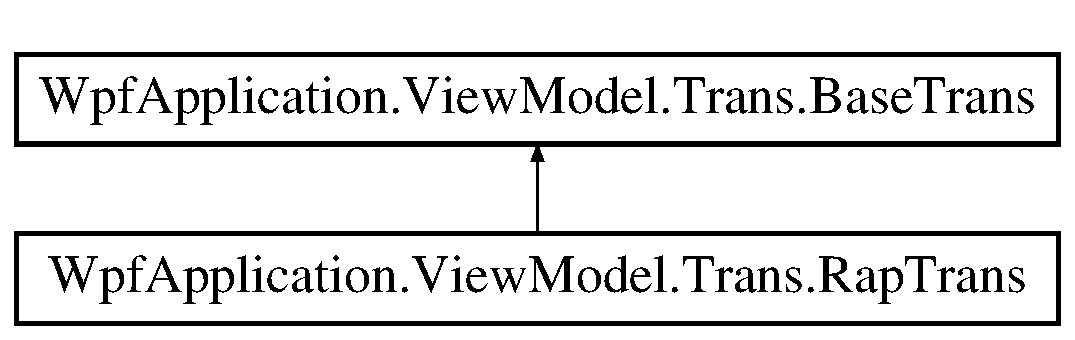
\includegraphics[height=2.000000cm]{class_wpf_application_1_1_view_model_1_1_trans_1_1_rap_trans}
\end{center}
\end{figure}
\subsection*{Public Member Functions}
\begin{DoxyCompactItemize}
\item 
\hyperlink{class_wpf_application_1_1_view_model_1_1_trans_1_1_rap_trans_aba3e175b49d344cb2f9a640dca1aceba}{Rap\-Trans} (int mat, string prat, string \hyperlink{class_wpf_application_1_1_view_model_1_1_trans_1_1_rap_trans_ad562e5cf54632e117c242e7a1904c842}{date})
\item 
override string \hyperlink{class_wpf_application_1_1_view_model_1_1_trans_1_1_rap_trans_a1b602f2f0fe337f5c8c4e2b02a952e2c}{To\-String} ()
\item 
string \hyperlink{class_wpf_application_1_1_view_model_1_1_trans_1_1_rap_trans_a1e91573fc69c94a7817d46d7808ab22b}{To\-Csv\-Row} ()
\begin{DoxyCompactList}\small\item\em Retourne une representation de l'instance sous forme d'une string, ligne d'un fichier C\-S\-V. Format\-: \char`\"{}col1;col2;col2\textbackslash{}n\char`\"{} \end{DoxyCompactList}\item 
override string \hyperlink{class_wpf_application_1_1_view_model_1_1_trans_1_1_rap_trans_acbc5326d57143463f3d26fe66dab7a14}{get\-Class} ()
\end{DoxyCompactItemize}
\subsection*{Properties}
\begin{DoxyCompactItemize}
\item 
int \hyperlink{class_wpf_application_1_1_view_model_1_1_trans_1_1_rap_trans_a6f637f8b8031dc3b044e5d21a96a019d}{numero}\hspace{0.3cm}{\ttfamily  \mbox{[}get, set\mbox{]}}
\item 
string \hyperlink{class_wpf_application_1_1_view_model_1_1_trans_1_1_rap_trans_a288e17d16695cf138271c000d8aa652e}{praticien}\hspace{0.3cm}{\ttfamily  \mbox{[}get, set\mbox{]}}
\item 
string \hyperlink{class_wpf_application_1_1_view_model_1_1_trans_1_1_rap_trans_ad562e5cf54632e117c242e7a1904c842}{date}\hspace{0.3cm}{\ttfamily  \mbox{[}get, set\mbox{]}}
\end{DoxyCompactItemize}


\subsection{Constructor \& Destructor Documentation}
\hypertarget{class_wpf_application_1_1_view_model_1_1_trans_1_1_rap_trans_aba3e175b49d344cb2f9a640dca1aceba}{\index{Wpf\-Application\-::\-View\-Model\-::\-Trans\-::\-Rap\-Trans@{Wpf\-Application\-::\-View\-Model\-::\-Trans\-::\-Rap\-Trans}!Rap\-Trans@{Rap\-Trans}}
\index{Rap\-Trans@{Rap\-Trans}!WpfApplication::ViewModel::Trans::RapTrans@{Wpf\-Application\-::\-View\-Model\-::\-Trans\-::\-Rap\-Trans}}
\subsubsection[{Rap\-Trans}]{\setlength{\rightskip}{0pt plus 5cm}Wpf\-Application.\-View\-Model.\-Trans.\-Rap\-Trans.\-Rap\-Trans (
\begin{DoxyParamCaption}
\item[{int}]{mat, }
\item[{string}]{prat, }
\item[{string}]{date}
\end{DoxyParamCaption}
)}}\label{class_wpf_application_1_1_view_model_1_1_trans_1_1_rap_trans_aba3e175b49d344cb2f9a640dca1aceba}


\subsection{Member Function Documentation}
\hypertarget{class_wpf_application_1_1_view_model_1_1_trans_1_1_rap_trans_acbc5326d57143463f3d26fe66dab7a14}{\index{Wpf\-Application\-::\-View\-Model\-::\-Trans\-::\-Rap\-Trans@{Wpf\-Application\-::\-View\-Model\-::\-Trans\-::\-Rap\-Trans}!get\-Class@{get\-Class}}
\index{get\-Class@{get\-Class}!WpfApplication::ViewModel::Trans::RapTrans@{Wpf\-Application\-::\-View\-Model\-::\-Trans\-::\-Rap\-Trans}}
\subsubsection[{get\-Class}]{\setlength{\rightskip}{0pt plus 5cm}override string Wpf\-Application.\-View\-Model.\-Trans.\-Rap\-Trans.\-get\-Class (
\begin{DoxyParamCaption}
{}
\end{DoxyParamCaption}
)\hspace{0.3cm}{\ttfamily [virtual]}}}\label{class_wpf_application_1_1_view_model_1_1_trans_1_1_rap_trans_acbc5326d57143463f3d26fe66dab7a14}


Reimplemented from \hyperlink{class_wpf_application_1_1_view_model_1_1_trans_1_1_base_trans_a9660be8cb25ed5d666eab9ddd10600aa}{Wpf\-Application.\-View\-Model.\-Trans.\-Base\-Trans}.

\hypertarget{class_wpf_application_1_1_view_model_1_1_trans_1_1_rap_trans_a1e91573fc69c94a7817d46d7808ab22b}{\index{Wpf\-Application\-::\-View\-Model\-::\-Trans\-::\-Rap\-Trans@{Wpf\-Application\-::\-View\-Model\-::\-Trans\-::\-Rap\-Trans}!To\-Csv\-Row@{To\-Csv\-Row}}
\index{To\-Csv\-Row@{To\-Csv\-Row}!WpfApplication::ViewModel::Trans::RapTrans@{Wpf\-Application\-::\-View\-Model\-::\-Trans\-::\-Rap\-Trans}}
\subsubsection[{To\-Csv\-Row}]{\setlength{\rightskip}{0pt plus 5cm}string Wpf\-Application.\-View\-Model.\-Trans.\-Rap\-Trans.\-To\-Csv\-Row (
\begin{DoxyParamCaption}
{}
\end{DoxyParamCaption}
)}}\label{class_wpf_application_1_1_view_model_1_1_trans_1_1_rap_trans_a1e91573fc69c94a7817d46d7808ab22b}


Retourne une representation de l'instance sous forme d'une string, ligne d'un fichier C\-S\-V. Format\-: \char`\"{}col1;col2;col2\textbackslash{}n\char`\"{} 

\begin{DoxyReturn}{Returns}
String, separee par des ';' et terminee par '\par
'
\end{DoxyReturn}
\hypertarget{class_wpf_application_1_1_view_model_1_1_trans_1_1_rap_trans_a1b602f2f0fe337f5c8c4e2b02a952e2c}{\index{Wpf\-Application\-::\-View\-Model\-::\-Trans\-::\-Rap\-Trans@{Wpf\-Application\-::\-View\-Model\-::\-Trans\-::\-Rap\-Trans}!To\-String@{To\-String}}
\index{To\-String@{To\-String}!WpfApplication::ViewModel::Trans::RapTrans@{Wpf\-Application\-::\-View\-Model\-::\-Trans\-::\-Rap\-Trans}}
\subsubsection[{To\-String}]{\setlength{\rightskip}{0pt plus 5cm}override string Wpf\-Application.\-View\-Model.\-Trans.\-Rap\-Trans.\-To\-String (
\begin{DoxyParamCaption}
{}
\end{DoxyParamCaption}
)}}\label{class_wpf_application_1_1_view_model_1_1_trans_1_1_rap_trans_a1b602f2f0fe337f5c8c4e2b02a952e2c}


\subsection{Property Documentation}
\hypertarget{class_wpf_application_1_1_view_model_1_1_trans_1_1_rap_trans_ad562e5cf54632e117c242e7a1904c842}{\index{Wpf\-Application\-::\-View\-Model\-::\-Trans\-::\-Rap\-Trans@{Wpf\-Application\-::\-View\-Model\-::\-Trans\-::\-Rap\-Trans}!date@{date}}
\index{date@{date}!WpfApplication::ViewModel::Trans::RapTrans@{Wpf\-Application\-::\-View\-Model\-::\-Trans\-::\-Rap\-Trans}}
\subsubsection[{date}]{\setlength{\rightskip}{0pt plus 5cm}string Wpf\-Application.\-View\-Model.\-Trans.\-Rap\-Trans.\-date\hspace{0.3cm}{\ttfamily [get]}, {\ttfamily [set]}}}\label{class_wpf_application_1_1_view_model_1_1_trans_1_1_rap_trans_ad562e5cf54632e117c242e7a1904c842}
\hypertarget{class_wpf_application_1_1_view_model_1_1_trans_1_1_rap_trans_a6f637f8b8031dc3b044e5d21a96a019d}{\index{Wpf\-Application\-::\-View\-Model\-::\-Trans\-::\-Rap\-Trans@{Wpf\-Application\-::\-View\-Model\-::\-Trans\-::\-Rap\-Trans}!numero@{numero}}
\index{numero@{numero}!WpfApplication::ViewModel::Trans::RapTrans@{Wpf\-Application\-::\-View\-Model\-::\-Trans\-::\-Rap\-Trans}}
\subsubsection[{numero}]{\setlength{\rightskip}{0pt plus 5cm}int Wpf\-Application.\-View\-Model.\-Trans.\-Rap\-Trans.\-numero\hspace{0.3cm}{\ttfamily [get]}, {\ttfamily [set]}}}\label{class_wpf_application_1_1_view_model_1_1_trans_1_1_rap_trans_a6f637f8b8031dc3b044e5d21a96a019d}
\hypertarget{class_wpf_application_1_1_view_model_1_1_trans_1_1_rap_trans_a288e17d16695cf138271c000d8aa652e}{\index{Wpf\-Application\-::\-View\-Model\-::\-Trans\-::\-Rap\-Trans@{Wpf\-Application\-::\-View\-Model\-::\-Trans\-::\-Rap\-Trans}!praticien@{praticien}}
\index{praticien@{praticien}!WpfApplication::ViewModel::Trans::RapTrans@{Wpf\-Application\-::\-View\-Model\-::\-Trans\-::\-Rap\-Trans}}
\subsubsection[{praticien}]{\setlength{\rightskip}{0pt plus 5cm}string Wpf\-Application.\-View\-Model.\-Trans.\-Rap\-Trans.\-praticien\hspace{0.3cm}{\ttfamily [get]}, {\ttfamily [set]}}}\label{class_wpf_application_1_1_view_model_1_1_trans_1_1_rap_trans_a288e17d16695cf138271c000d8aa652e}


The documentation for this class was generated from the following file\-:\begin{DoxyCompactItemize}
\item 
C\-:/\-Users/dju/\-Documents/\-Visual Studio 2012/\-Projects/\-P\-P\-E/\-P\-P\-E3/\-Wpf\-Application/\-View\-Model/\-Trans/\hyperlink{_rap_trans_8cs}{Rap\-Trans.\-cs}\end{DoxyCompactItemize}

\hypertarget{class_model_1_1_r_e_g_i_o_n}{\section{Model.\-R\-E\-G\-I\-O\-N Class Reference}
\label{class_model_1_1_r_e_g_i_o_n}\index{Model.\-R\-E\-G\-I\-O\-N@{Model.\-R\-E\-G\-I\-O\-N}}
}


Aucune documentation sur les métadonnées n'est disponible.  


Inheritance diagram for Model.\-R\-E\-G\-I\-O\-N\-:\begin{figure}[H]
\begin{center}
\leavevmode
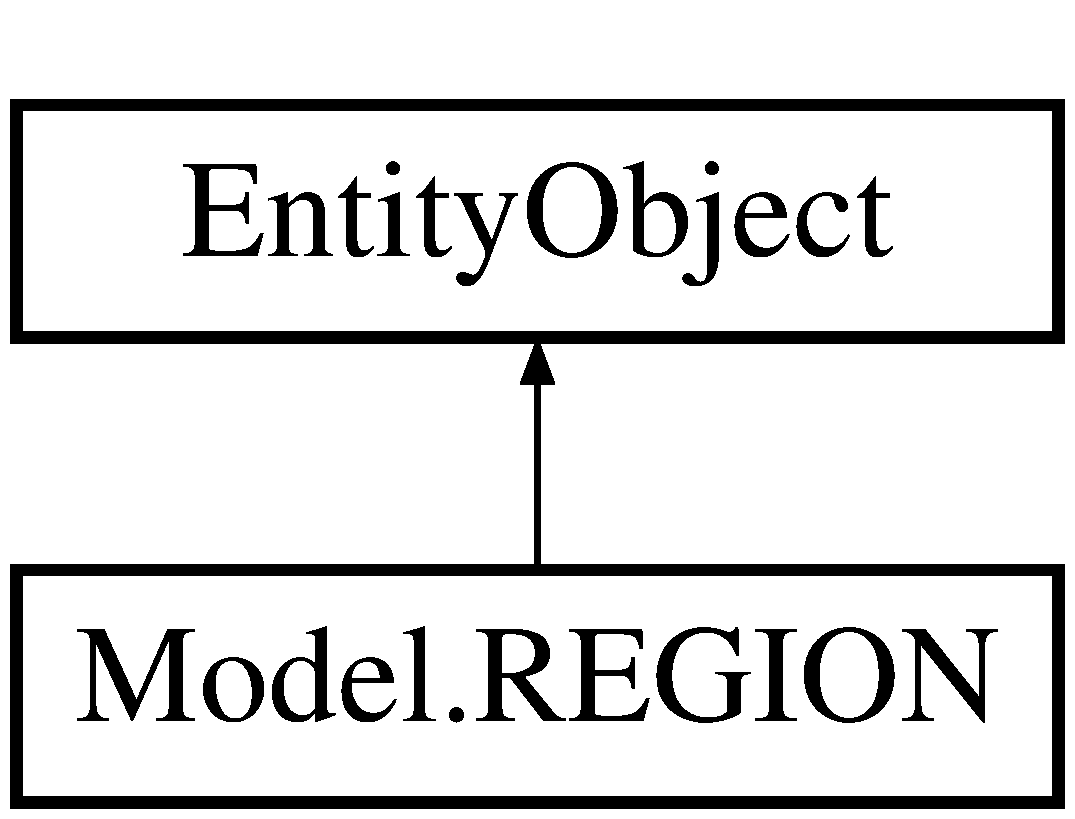
\includegraphics[height=2.000000cm]{class_model_1_1_r_e_g_i_o_n}
\end{center}
\end{figure}
\subsection*{Static Public Member Functions}
\begin{DoxyCompactItemize}
\item 
static \hyperlink{class_model_1_1_r_e_g_i_o_n}{R\-E\-G\-I\-O\-N} \hyperlink{class_model_1_1_r_e_g_i_o_n_a5d9c4388644568f676a3687a11c8c3b6}{Create\-R\-E\-G\-I\-O\-N} (global\-::\-System.\-String \hyperlink{class_model_1_1_r_e_g_i_o_n_a7c0fd7797a562f170daff2673177dc83}{code\-\_\-region}, global\-::\-System.\-String \hyperlink{class_model_1_1_r_e_g_i_o_n_a4dceb2c8c2a0b59bd07caba731ff984a}{nom\-\_\-region})
\begin{DoxyCompactList}\small\item\em Créez un nouvel objet \hyperlink{class_model_1_1_r_e_g_i_o_n}{R\-E\-G\-I\-O\-N}. \end{DoxyCompactList}\end{DoxyCompactItemize}
\subsection*{Properties}
\begin{DoxyCompactItemize}
\item 
global\-::\-System.\-String \hyperlink{class_model_1_1_r_e_g_i_o_n_a7c0fd7797a562f170daff2673177dc83}{code\-\_\-region}\hspace{0.3cm}{\ttfamily  \mbox{[}get, set\mbox{]}}
\begin{DoxyCompactList}\small\item\em Aucune documentation sur les métadonnées n'est disponible. \end{DoxyCompactList}\item 
global\-::\-System.\-String \hyperlink{class_model_1_1_r_e_g_i_o_n_a8a17b4d46de541201536619d69596c90}{code\-\_\-secteur}\hspace{0.3cm}{\ttfamily  \mbox{[}get, set\mbox{]}}
\begin{DoxyCompactList}\small\item\em Aucune documentation sur les métadonnées n'est disponible. \end{DoxyCompactList}\item 
global\-::\-System.\-String \hyperlink{class_model_1_1_r_e_g_i_o_n_a4dceb2c8c2a0b59bd07caba731ff984a}{nom\-\_\-region}\hspace{0.3cm}{\ttfamily  \mbox{[}get, set\mbox{]}}
\begin{DoxyCompactList}\small\item\em Aucune documentation sur les métadonnées n'est disponible. \end{DoxyCompactList}\item 
Entity\-Collection$<$ \hyperlink{class_model_1_1_d_e_p_a_r_t_e_m_e_n_t}{D\-E\-P\-A\-R\-T\-E\-M\-E\-N\-T} $>$ \hyperlink{class_model_1_1_r_e_g_i_o_n_a4c03f8b282035bb407ba160cd96ea51f}{D\-E\-P\-A\-R\-T\-E\-M\-E\-N\-T}\hspace{0.3cm}{\ttfamily  \mbox{[}get, set\mbox{]}}
\begin{DoxyCompactList}\small\item\em Aucune documentation sur les métadonnées n'est disponible. \end{DoxyCompactList}\item 
Entity\-Collection$<$ \hyperlink{class_model_1_1_g_e_r_e}{G\-E\-R\-E} $>$ \hyperlink{class_model_1_1_r_e_g_i_o_n_a331f4581a87b7e6d2b23377530395efa}{G\-E\-R\-E}\hspace{0.3cm}{\ttfamily  \mbox{[}get, set\mbox{]}}
\begin{DoxyCompactList}\small\item\em Aucune documentation sur les métadonnées n'est disponible. \end{DoxyCompactList}\item 
Entity\-Collection$<$ \hyperlink{class_model_1_1_v_i_s_i_t_e_u_r}{V\-I\-S\-I\-T\-E\-U\-R} $>$ \hyperlink{class_model_1_1_r_e_g_i_o_n_a41de25bdbbf292c65117c12cc2348bf8}{V\-I\-S\-I\-T\-E\-U\-R}\hspace{0.3cm}{\ttfamily  \mbox{[}get, set\mbox{]}}
\begin{DoxyCompactList}\small\item\em Aucune documentation sur les métadonnées n'est disponible. \end{DoxyCompactList}\item 
\hyperlink{class_model_1_1_s_e_c_t_e_u_r}{S\-E\-C\-T\-E\-U\-R} \hyperlink{class_model_1_1_r_e_g_i_o_n_a1a0c5b20ed4f339d95de08844b77b5b6}{S\-E\-C\-T\-E\-U\-R}\hspace{0.3cm}{\ttfamily  \mbox{[}get, set\mbox{]}}
\begin{DoxyCompactList}\small\item\em Aucune documentation sur les métadonnées n'est disponible. \end{DoxyCompactList}\item 
Entity\-Reference$<$ \hyperlink{class_model_1_1_s_e_c_t_e_u_r}{S\-E\-C\-T\-E\-U\-R} $>$ \hyperlink{class_model_1_1_r_e_g_i_o_n_a30e268a49e6d95f6de38d81b420fc3b3}{S\-E\-C\-T\-E\-U\-R\-Reference}\hspace{0.3cm}{\ttfamily  \mbox{[}get, set\mbox{]}}
\begin{DoxyCompactList}\small\item\em Aucune documentation sur les métadonnées n'est disponible. \end{DoxyCompactList}\end{DoxyCompactItemize}


\subsection{Detailed Description}
Aucune documentation sur les métadonnées n'est disponible. 



\subsection{Member Function Documentation}
\hypertarget{class_model_1_1_r_e_g_i_o_n_a5d9c4388644568f676a3687a11c8c3b6}{\index{Model\-::\-R\-E\-G\-I\-O\-N@{Model\-::\-R\-E\-G\-I\-O\-N}!Create\-R\-E\-G\-I\-O\-N@{Create\-R\-E\-G\-I\-O\-N}}
\index{Create\-R\-E\-G\-I\-O\-N@{Create\-R\-E\-G\-I\-O\-N}!Model::REGION@{Model\-::\-R\-E\-G\-I\-O\-N}}
\subsubsection[{Create\-R\-E\-G\-I\-O\-N}]{\setlength{\rightskip}{0pt plus 5cm}static {\bf R\-E\-G\-I\-O\-N} Model.\-R\-E\-G\-I\-O\-N.\-Create\-R\-E\-G\-I\-O\-N (
\begin{DoxyParamCaption}
\item[{global\-::\-System.\-String}]{code\-\_\-region, }
\item[{global\-::\-System.\-String}]{nom\-\_\-region}
\end{DoxyParamCaption}
)\hspace{0.3cm}{\ttfamily [static]}}}\label{class_model_1_1_r_e_g_i_o_n_a5d9c4388644568f676a3687a11c8c3b6}


Créez un nouvel objet \hyperlink{class_model_1_1_r_e_g_i_o_n}{R\-E\-G\-I\-O\-N}. 


\begin{DoxyParams}{Parameters}
{\em code\-\_\-region} & Valeur initiale de la propriété code\-\_\-region.\\
\hline
{\em nom\-\_\-region} & Valeur initiale de la propriété nom\-\_\-region.\\
\hline
\end{DoxyParams}


\subsection{Property Documentation}
\hypertarget{class_model_1_1_r_e_g_i_o_n_a7c0fd7797a562f170daff2673177dc83}{\index{Model\-::\-R\-E\-G\-I\-O\-N@{Model\-::\-R\-E\-G\-I\-O\-N}!code\-\_\-region@{code\-\_\-region}}
\index{code\-\_\-region@{code\-\_\-region}!Model::REGION@{Model\-::\-R\-E\-G\-I\-O\-N}}
\subsubsection[{code\-\_\-region}]{\setlength{\rightskip}{0pt plus 5cm}global.\-System.\-String Model.\-R\-E\-G\-I\-O\-N.\-code\-\_\-region\hspace{0.3cm}{\ttfamily [get]}, {\ttfamily [set]}}}\label{class_model_1_1_r_e_g_i_o_n_a7c0fd7797a562f170daff2673177dc83}


Aucune documentation sur les métadonnées n'est disponible. 

\hypertarget{class_model_1_1_r_e_g_i_o_n_a8a17b4d46de541201536619d69596c90}{\index{Model\-::\-R\-E\-G\-I\-O\-N@{Model\-::\-R\-E\-G\-I\-O\-N}!code\-\_\-secteur@{code\-\_\-secteur}}
\index{code\-\_\-secteur@{code\-\_\-secteur}!Model::REGION@{Model\-::\-R\-E\-G\-I\-O\-N}}
\subsubsection[{code\-\_\-secteur}]{\setlength{\rightskip}{0pt plus 5cm}global.\-System.\-String Model.\-R\-E\-G\-I\-O\-N.\-code\-\_\-secteur\hspace{0.3cm}{\ttfamily [get]}, {\ttfamily [set]}}}\label{class_model_1_1_r_e_g_i_o_n_a8a17b4d46de541201536619d69596c90}


Aucune documentation sur les métadonnées n'est disponible. 

\hypertarget{class_model_1_1_r_e_g_i_o_n_a4c03f8b282035bb407ba160cd96ea51f}{\index{Model\-::\-R\-E\-G\-I\-O\-N@{Model\-::\-R\-E\-G\-I\-O\-N}!D\-E\-P\-A\-R\-T\-E\-M\-E\-N\-T@{D\-E\-P\-A\-R\-T\-E\-M\-E\-N\-T}}
\index{D\-E\-P\-A\-R\-T\-E\-M\-E\-N\-T@{D\-E\-P\-A\-R\-T\-E\-M\-E\-N\-T}!Model::REGION@{Model\-::\-R\-E\-G\-I\-O\-N}}
\subsubsection[{D\-E\-P\-A\-R\-T\-E\-M\-E\-N\-T}]{\setlength{\rightskip}{0pt plus 5cm}Entity\-Collection$<${\bf D\-E\-P\-A\-R\-T\-E\-M\-E\-N\-T}$>$ Model.\-R\-E\-G\-I\-O\-N.\-D\-E\-P\-A\-R\-T\-E\-M\-E\-N\-T\hspace{0.3cm}{\ttfamily [get]}, {\ttfamily [set]}}}\label{class_model_1_1_r_e_g_i_o_n_a4c03f8b282035bb407ba160cd96ea51f}


Aucune documentation sur les métadonnées n'est disponible. 

\hypertarget{class_model_1_1_r_e_g_i_o_n_a331f4581a87b7e6d2b23377530395efa}{\index{Model\-::\-R\-E\-G\-I\-O\-N@{Model\-::\-R\-E\-G\-I\-O\-N}!G\-E\-R\-E@{G\-E\-R\-E}}
\index{G\-E\-R\-E@{G\-E\-R\-E}!Model::REGION@{Model\-::\-R\-E\-G\-I\-O\-N}}
\subsubsection[{G\-E\-R\-E}]{\setlength{\rightskip}{0pt plus 5cm}Entity\-Collection$<${\bf G\-E\-R\-E}$>$ Model.\-R\-E\-G\-I\-O\-N.\-G\-E\-R\-E\hspace{0.3cm}{\ttfamily [get]}, {\ttfamily [set]}}}\label{class_model_1_1_r_e_g_i_o_n_a331f4581a87b7e6d2b23377530395efa}


Aucune documentation sur les métadonnées n'est disponible. 

\hypertarget{class_model_1_1_r_e_g_i_o_n_a4dceb2c8c2a0b59bd07caba731ff984a}{\index{Model\-::\-R\-E\-G\-I\-O\-N@{Model\-::\-R\-E\-G\-I\-O\-N}!nom\-\_\-region@{nom\-\_\-region}}
\index{nom\-\_\-region@{nom\-\_\-region}!Model::REGION@{Model\-::\-R\-E\-G\-I\-O\-N}}
\subsubsection[{nom\-\_\-region}]{\setlength{\rightskip}{0pt plus 5cm}global.\-System.\-String Model.\-R\-E\-G\-I\-O\-N.\-nom\-\_\-region\hspace{0.3cm}{\ttfamily [get]}, {\ttfamily [set]}}}\label{class_model_1_1_r_e_g_i_o_n_a4dceb2c8c2a0b59bd07caba731ff984a}


Aucune documentation sur les métadonnées n'est disponible. 

\hypertarget{class_model_1_1_r_e_g_i_o_n_a1a0c5b20ed4f339d95de08844b77b5b6}{\index{Model\-::\-R\-E\-G\-I\-O\-N@{Model\-::\-R\-E\-G\-I\-O\-N}!S\-E\-C\-T\-E\-U\-R@{S\-E\-C\-T\-E\-U\-R}}
\index{S\-E\-C\-T\-E\-U\-R@{S\-E\-C\-T\-E\-U\-R}!Model::REGION@{Model\-::\-R\-E\-G\-I\-O\-N}}
\subsubsection[{S\-E\-C\-T\-E\-U\-R}]{\setlength{\rightskip}{0pt plus 5cm}{\bf S\-E\-C\-T\-E\-U\-R} Model.\-R\-E\-G\-I\-O\-N.\-S\-E\-C\-T\-E\-U\-R\hspace{0.3cm}{\ttfamily [get]}, {\ttfamily [set]}}}\label{class_model_1_1_r_e_g_i_o_n_a1a0c5b20ed4f339d95de08844b77b5b6}


Aucune documentation sur les métadonnées n'est disponible. 

\hypertarget{class_model_1_1_r_e_g_i_o_n_a30e268a49e6d95f6de38d81b420fc3b3}{\index{Model\-::\-R\-E\-G\-I\-O\-N@{Model\-::\-R\-E\-G\-I\-O\-N}!S\-E\-C\-T\-E\-U\-R\-Reference@{S\-E\-C\-T\-E\-U\-R\-Reference}}
\index{S\-E\-C\-T\-E\-U\-R\-Reference@{S\-E\-C\-T\-E\-U\-R\-Reference}!Model::REGION@{Model\-::\-R\-E\-G\-I\-O\-N}}
\subsubsection[{S\-E\-C\-T\-E\-U\-R\-Reference}]{\setlength{\rightskip}{0pt plus 5cm}Entity\-Reference$<${\bf S\-E\-C\-T\-E\-U\-R}$>$ Model.\-R\-E\-G\-I\-O\-N.\-S\-E\-C\-T\-E\-U\-R\-Reference\hspace{0.3cm}{\ttfamily [get]}, {\ttfamily [set]}}}\label{class_model_1_1_r_e_g_i_o_n_a30e268a49e6d95f6de38d81b420fc3b3}


Aucune documentation sur les métadonnées n'est disponible. 

\hypertarget{class_model_1_1_r_e_g_i_o_n_a41de25bdbbf292c65117c12cc2348bf8}{\index{Model\-::\-R\-E\-G\-I\-O\-N@{Model\-::\-R\-E\-G\-I\-O\-N}!V\-I\-S\-I\-T\-E\-U\-R@{V\-I\-S\-I\-T\-E\-U\-R}}
\index{V\-I\-S\-I\-T\-E\-U\-R@{V\-I\-S\-I\-T\-E\-U\-R}!Model::REGION@{Model\-::\-R\-E\-G\-I\-O\-N}}
\subsubsection[{V\-I\-S\-I\-T\-E\-U\-R}]{\setlength{\rightskip}{0pt plus 5cm}Entity\-Collection$<${\bf V\-I\-S\-I\-T\-E\-U\-R}$>$ Model.\-R\-E\-G\-I\-O\-N.\-V\-I\-S\-I\-T\-E\-U\-R\hspace{0.3cm}{\ttfamily [get]}, {\ttfamily [set]}}}\label{class_model_1_1_r_e_g_i_o_n_a41de25bdbbf292c65117c12cc2348bf8}


Aucune documentation sur les métadonnées n'est disponible. 



The documentation for this class was generated from the following file\-:\begin{DoxyCompactItemize}
\item 
C\-:/\-Users/dju/\-Documents/\-Visual Studio 2012/\-Projects/\-P\-P\-E/\-P\-P\-E3/\-Model/\hyperlink{_model_bdd_sio_8_designer_8cs}{Model\-Bdd\-Sio.\-Designer.\-cs}\end{DoxyCompactItemize}

\hypertarget{class_model_1_1_r_e_m_p_l_a_c_e}{\section{Model.\-R\-E\-M\-P\-L\-A\-C\-E Class Reference}
\label{class_model_1_1_r_e_m_p_l_a_c_e}\index{Model.\-R\-E\-M\-P\-L\-A\-C\-E@{Model.\-R\-E\-M\-P\-L\-A\-C\-E}}
}


Aucune documentation sur les métadonnées n'est disponible.  


Inheritance diagram for Model.\-R\-E\-M\-P\-L\-A\-C\-E\-:\begin{figure}[H]
\begin{center}
\leavevmode
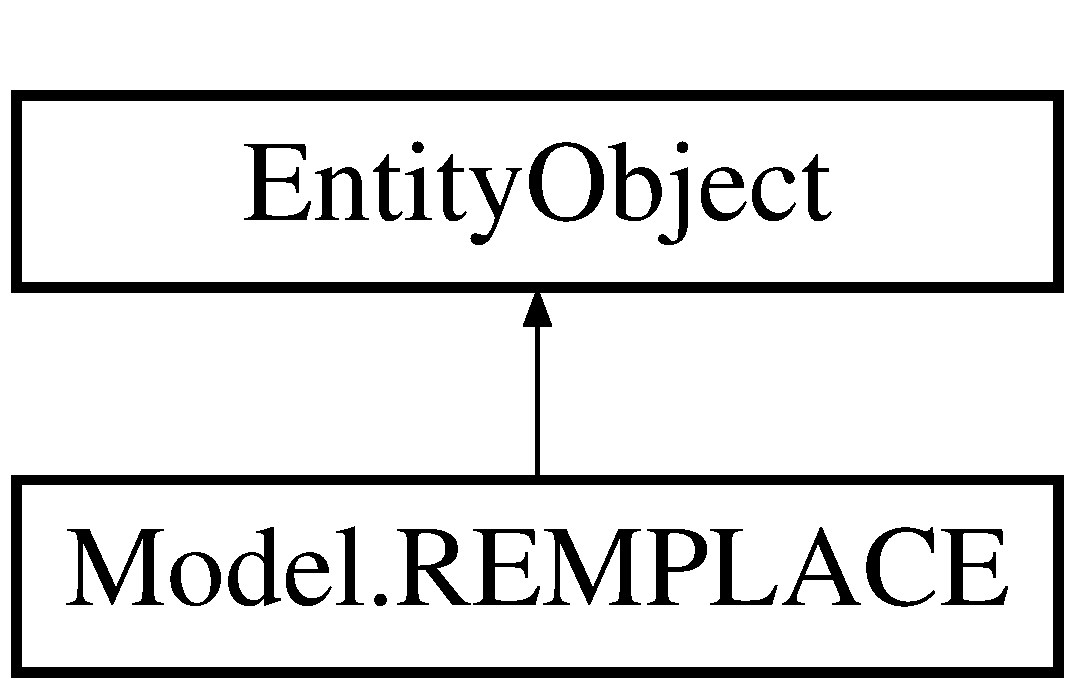
\includegraphics[height=2.000000cm]{class_model_1_1_r_e_m_p_l_a_c_e}
\end{center}
\end{figure}
\subsection*{Static Public Member Functions}
\begin{DoxyCompactItemize}
\item 
static \hyperlink{class_model_1_1_r_e_m_p_l_a_c_e}{R\-E\-M\-P\-L\-A\-C\-E} \hyperlink{class_model_1_1_r_e_m_p_l_a_c_e_adf148310a39f025b9b9f4c643eb2e89c}{Create\-R\-E\-M\-P\-L\-A\-C\-E} (global\-::\-System.\-Int32 \hyperlink{class_model_1_1_r_e_m_p_l_a_c_e_ac3e241e1a97864f915ca369bd99dfde3}{matricule\-\_\-praticien\-\_\-remplace}, global\-::\-System.\-Int32 \hyperlink{class_model_1_1_r_e_m_p_l_a_c_e_a43176ce5aac61a5dbb677d871f8f2c32}{matricule\-\_\-praticien\-\_\-remplacant}, global\-::\-System.\-Date\-Time j\-J\-M\-M\-A\-A\-A\-A)
\begin{DoxyCompactList}\small\item\em Créez un nouvel objet \hyperlink{class_model_1_1_r_e_m_p_l_a_c_e}{R\-E\-M\-P\-L\-A\-C\-E}. \end{DoxyCompactList}\end{DoxyCompactItemize}
\subsection*{Properties}
\begin{DoxyCompactItemize}
\item 
global\-::\-System.\-Int32 \hyperlink{class_model_1_1_r_e_m_p_l_a_c_e_ac3e241e1a97864f915ca369bd99dfde3}{matricule\-\_\-praticien\-\_\-remplace}\hspace{0.3cm}{\ttfamily  \mbox{[}get, set\mbox{]}}
\begin{DoxyCompactList}\small\item\em Aucune documentation sur les métadonnées n'est disponible. \end{DoxyCompactList}\item 
global\-::\-System.\-Int32 \hyperlink{class_model_1_1_r_e_m_p_l_a_c_e_a43176ce5aac61a5dbb677d871f8f2c32}{matricule\-\_\-praticien\-\_\-remplacant}\hspace{0.3cm}{\ttfamily  \mbox{[}get, set\mbox{]}}
\begin{DoxyCompactList}\small\item\em Aucune documentation sur les métadonnées n'est disponible. \end{DoxyCompactList}\item 
global\-::\-System.\-Date\-Time \hyperlink{class_model_1_1_r_e_m_p_l_a_c_e_add9e25bf7035011a33a3891f38094899}{J\-J\-M\-M\-A\-A\-A\-A}\hspace{0.3cm}{\ttfamily  \mbox{[}get, set\mbox{]}}
\begin{DoxyCompactList}\small\item\em Aucune documentation sur les métadonnées n'est disponible. \end{DoxyCompactList}\item 
\hyperlink{class_model_1_1_d_a_t_e}{D\-A\-T\-E} \hyperlink{class_model_1_1_r_e_m_p_l_a_c_e_aa79608c4a3babab2a00e7d15e39a0000}{D\-A\-T\-E}\hspace{0.3cm}{\ttfamily  \mbox{[}get, set\mbox{]}}
\begin{DoxyCompactList}\small\item\em Aucune documentation sur les métadonnées n'est disponible. \end{DoxyCompactList}\item 
Entity\-Reference$<$ \hyperlink{class_model_1_1_d_a_t_e}{D\-A\-T\-E} $>$ \hyperlink{class_model_1_1_r_e_m_p_l_a_c_e_abf3a8737719c75494fa54c1ffe335d39}{D\-A\-T\-E\-Reference}\hspace{0.3cm}{\ttfamily  \mbox{[}get, set\mbox{]}}
\begin{DoxyCompactList}\small\item\em Aucune documentation sur les métadonnées n'est disponible. \end{DoxyCompactList}\item 
\hyperlink{class_model_1_1_p_r_a_t_i_c_i_e_n}{P\-R\-A\-T\-I\-C\-I\-E\-N} \hyperlink{class_model_1_1_r_e_m_p_l_a_c_e_ae390942d049897645a0751dda7578846}{P\-R\-A\-T\-I\-C\-I\-E\-N}\hspace{0.3cm}{\ttfamily  \mbox{[}get, set\mbox{]}}
\begin{DoxyCompactList}\small\item\em Aucune documentation sur les métadonnées n'est disponible. \end{DoxyCompactList}\item 
Entity\-Reference$<$ \hyperlink{class_model_1_1_p_r_a_t_i_c_i_e_n}{P\-R\-A\-T\-I\-C\-I\-E\-N} $>$ \hyperlink{class_model_1_1_r_e_m_p_l_a_c_e_ae00edbfe75242bb1d02e1315c5cdacd8}{P\-R\-A\-T\-I\-C\-I\-E\-N\-Reference}\hspace{0.3cm}{\ttfamily  \mbox{[}get, set\mbox{]}}
\begin{DoxyCompactList}\small\item\em Aucune documentation sur les métadonnées n'est disponible. \end{DoxyCompactList}\item 
\hyperlink{class_model_1_1_p_r_a_t_i_c_i_e_n}{P\-R\-A\-T\-I\-C\-I\-E\-N} \hyperlink{class_model_1_1_r_e_m_p_l_a_c_e_a4a071b1a7be7992a57e0f67876808145}{P\-R\-A\-T\-I\-C\-I\-E\-N1}\hspace{0.3cm}{\ttfamily  \mbox{[}get, set\mbox{]}}
\begin{DoxyCompactList}\small\item\em Aucune documentation sur les métadonnées n'est disponible. \end{DoxyCompactList}\item 
Entity\-Reference$<$ \hyperlink{class_model_1_1_p_r_a_t_i_c_i_e_n}{P\-R\-A\-T\-I\-C\-I\-E\-N} $>$ \hyperlink{class_model_1_1_r_e_m_p_l_a_c_e_a57e1924ffc9f114166ef3cd638f600af}{P\-R\-A\-T\-I\-C\-I\-E\-N1\-Reference}\hspace{0.3cm}{\ttfamily  \mbox{[}get, set\mbox{]}}
\begin{DoxyCompactList}\small\item\em Aucune documentation sur les métadonnées n'est disponible. \end{DoxyCompactList}\end{DoxyCompactItemize}


\subsection{Detailed Description}
Aucune documentation sur les métadonnées n'est disponible. 



\subsection{Member Function Documentation}
\hypertarget{class_model_1_1_r_e_m_p_l_a_c_e_adf148310a39f025b9b9f4c643eb2e89c}{\index{Model\-::\-R\-E\-M\-P\-L\-A\-C\-E@{Model\-::\-R\-E\-M\-P\-L\-A\-C\-E}!Create\-R\-E\-M\-P\-L\-A\-C\-E@{Create\-R\-E\-M\-P\-L\-A\-C\-E}}
\index{Create\-R\-E\-M\-P\-L\-A\-C\-E@{Create\-R\-E\-M\-P\-L\-A\-C\-E}!Model::REMPLACE@{Model\-::\-R\-E\-M\-P\-L\-A\-C\-E}}
\subsubsection[{Create\-R\-E\-M\-P\-L\-A\-C\-E}]{\setlength{\rightskip}{0pt plus 5cm}static {\bf R\-E\-M\-P\-L\-A\-C\-E} Model.\-R\-E\-M\-P\-L\-A\-C\-E.\-Create\-R\-E\-M\-P\-L\-A\-C\-E (
\begin{DoxyParamCaption}
\item[{global\-::\-System.\-Int32}]{matricule\-\_\-praticien\-\_\-remplace, }
\item[{global\-::\-System.\-Int32}]{matricule\-\_\-praticien\-\_\-remplacant, }
\item[{global\-::\-System.\-Date\-Time}]{j\-J\-M\-M\-A\-A\-A\-A}
\end{DoxyParamCaption}
)\hspace{0.3cm}{\ttfamily [static]}}}\label{class_model_1_1_r_e_m_p_l_a_c_e_adf148310a39f025b9b9f4c643eb2e89c}


Créez un nouvel objet \hyperlink{class_model_1_1_r_e_m_p_l_a_c_e}{R\-E\-M\-P\-L\-A\-C\-E}. 


\begin{DoxyParams}{Parameters}
{\em matricule\-\_\-praticien\-\_\-remplace} & Valeur initiale de la propriété matricule\-\_\-praticien\-\_\-remplace.\\
\hline
{\em matricule\-\_\-praticien\-\_\-remplacant} & Valeur initiale de la propriété matricule\-\_\-praticien\-\_\-remplacant.\\
\hline
{\em j\-J\-M\-M\-A\-A\-A\-A} & Valeur initiale de la propriété J\-J\-M\-M\-A\-A\-A\-A.\\
\hline
\end{DoxyParams}


\subsection{Property Documentation}
\hypertarget{class_model_1_1_r_e_m_p_l_a_c_e_aa79608c4a3babab2a00e7d15e39a0000}{\index{Model\-::\-R\-E\-M\-P\-L\-A\-C\-E@{Model\-::\-R\-E\-M\-P\-L\-A\-C\-E}!D\-A\-T\-E@{D\-A\-T\-E}}
\index{D\-A\-T\-E@{D\-A\-T\-E}!Model::REMPLACE@{Model\-::\-R\-E\-M\-P\-L\-A\-C\-E}}
\subsubsection[{D\-A\-T\-E}]{\setlength{\rightskip}{0pt plus 5cm}{\bf D\-A\-T\-E} Model.\-R\-E\-M\-P\-L\-A\-C\-E.\-D\-A\-T\-E\hspace{0.3cm}{\ttfamily [get]}, {\ttfamily [set]}}}\label{class_model_1_1_r_e_m_p_l_a_c_e_aa79608c4a3babab2a00e7d15e39a0000}


Aucune documentation sur les métadonnées n'est disponible. 

\hypertarget{class_model_1_1_r_e_m_p_l_a_c_e_abf3a8737719c75494fa54c1ffe335d39}{\index{Model\-::\-R\-E\-M\-P\-L\-A\-C\-E@{Model\-::\-R\-E\-M\-P\-L\-A\-C\-E}!D\-A\-T\-E\-Reference@{D\-A\-T\-E\-Reference}}
\index{D\-A\-T\-E\-Reference@{D\-A\-T\-E\-Reference}!Model::REMPLACE@{Model\-::\-R\-E\-M\-P\-L\-A\-C\-E}}
\subsubsection[{D\-A\-T\-E\-Reference}]{\setlength{\rightskip}{0pt plus 5cm}Entity\-Reference$<${\bf D\-A\-T\-E}$>$ Model.\-R\-E\-M\-P\-L\-A\-C\-E.\-D\-A\-T\-E\-Reference\hspace{0.3cm}{\ttfamily [get]}, {\ttfamily [set]}}}\label{class_model_1_1_r_e_m_p_l_a_c_e_abf3a8737719c75494fa54c1ffe335d39}


Aucune documentation sur les métadonnées n'est disponible. 

\hypertarget{class_model_1_1_r_e_m_p_l_a_c_e_add9e25bf7035011a33a3891f38094899}{\index{Model\-::\-R\-E\-M\-P\-L\-A\-C\-E@{Model\-::\-R\-E\-M\-P\-L\-A\-C\-E}!J\-J\-M\-M\-A\-A\-A\-A@{J\-J\-M\-M\-A\-A\-A\-A}}
\index{J\-J\-M\-M\-A\-A\-A\-A@{J\-J\-M\-M\-A\-A\-A\-A}!Model::REMPLACE@{Model\-::\-R\-E\-M\-P\-L\-A\-C\-E}}
\subsubsection[{J\-J\-M\-M\-A\-A\-A\-A}]{\setlength{\rightskip}{0pt plus 5cm}global.\-System.\-Date\-Time Model.\-R\-E\-M\-P\-L\-A\-C\-E.\-J\-J\-M\-M\-A\-A\-A\-A\hspace{0.3cm}{\ttfamily [get]}, {\ttfamily [set]}}}\label{class_model_1_1_r_e_m_p_l_a_c_e_add9e25bf7035011a33a3891f38094899}


Aucune documentation sur les métadonnées n'est disponible. 

\hypertarget{class_model_1_1_r_e_m_p_l_a_c_e_a43176ce5aac61a5dbb677d871f8f2c32}{\index{Model\-::\-R\-E\-M\-P\-L\-A\-C\-E@{Model\-::\-R\-E\-M\-P\-L\-A\-C\-E}!matricule\-\_\-praticien\-\_\-remplacant@{matricule\-\_\-praticien\-\_\-remplacant}}
\index{matricule\-\_\-praticien\-\_\-remplacant@{matricule\-\_\-praticien\-\_\-remplacant}!Model::REMPLACE@{Model\-::\-R\-E\-M\-P\-L\-A\-C\-E}}
\subsubsection[{matricule\-\_\-praticien\-\_\-remplacant}]{\setlength{\rightskip}{0pt plus 5cm}global.\-System.\-Int32 Model.\-R\-E\-M\-P\-L\-A\-C\-E.\-matricule\-\_\-praticien\-\_\-remplacant\hspace{0.3cm}{\ttfamily [get]}, {\ttfamily [set]}}}\label{class_model_1_1_r_e_m_p_l_a_c_e_a43176ce5aac61a5dbb677d871f8f2c32}


Aucune documentation sur les métadonnées n'est disponible. 

\hypertarget{class_model_1_1_r_e_m_p_l_a_c_e_ac3e241e1a97864f915ca369bd99dfde3}{\index{Model\-::\-R\-E\-M\-P\-L\-A\-C\-E@{Model\-::\-R\-E\-M\-P\-L\-A\-C\-E}!matricule\-\_\-praticien\-\_\-remplace@{matricule\-\_\-praticien\-\_\-remplace}}
\index{matricule\-\_\-praticien\-\_\-remplace@{matricule\-\_\-praticien\-\_\-remplace}!Model::REMPLACE@{Model\-::\-R\-E\-M\-P\-L\-A\-C\-E}}
\subsubsection[{matricule\-\_\-praticien\-\_\-remplace}]{\setlength{\rightskip}{0pt plus 5cm}global.\-System.\-Int32 Model.\-R\-E\-M\-P\-L\-A\-C\-E.\-matricule\-\_\-praticien\-\_\-remplace\hspace{0.3cm}{\ttfamily [get]}, {\ttfamily [set]}}}\label{class_model_1_1_r_e_m_p_l_a_c_e_ac3e241e1a97864f915ca369bd99dfde3}


Aucune documentation sur les métadonnées n'est disponible. 

\hypertarget{class_model_1_1_r_e_m_p_l_a_c_e_ae390942d049897645a0751dda7578846}{\index{Model\-::\-R\-E\-M\-P\-L\-A\-C\-E@{Model\-::\-R\-E\-M\-P\-L\-A\-C\-E}!P\-R\-A\-T\-I\-C\-I\-E\-N@{P\-R\-A\-T\-I\-C\-I\-E\-N}}
\index{P\-R\-A\-T\-I\-C\-I\-E\-N@{P\-R\-A\-T\-I\-C\-I\-E\-N}!Model::REMPLACE@{Model\-::\-R\-E\-M\-P\-L\-A\-C\-E}}
\subsubsection[{P\-R\-A\-T\-I\-C\-I\-E\-N}]{\setlength{\rightskip}{0pt plus 5cm}{\bf P\-R\-A\-T\-I\-C\-I\-E\-N} Model.\-R\-E\-M\-P\-L\-A\-C\-E.\-P\-R\-A\-T\-I\-C\-I\-E\-N\hspace{0.3cm}{\ttfamily [get]}, {\ttfamily [set]}}}\label{class_model_1_1_r_e_m_p_l_a_c_e_ae390942d049897645a0751dda7578846}


Aucune documentation sur les métadonnées n'est disponible. 

\hypertarget{class_model_1_1_r_e_m_p_l_a_c_e_a4a071b1a7be7992a57e0f67876808145}{\index{Model\-::\-R\-E\-M\-P\-L\-A\-C\-E@{Model\-::\-R\-E\-M\-P\-L\-A\-C\-E}!P\-R\-A\-T\-I\-C\-I\-E\-N1@{P\-R\-A\-T\-I\-C\-I\-E\-N1}}
\index{P\-R\-A\-T\-I\-C\-I\-E\-N1@{P\-R\-A\-T\-I\-C\-I\-E\-N1}!Model::REMPLACE@{Model\-::\-R\-E\-M\-P\-L\-A\-C\-E}}
\subsubsection[{P\-R\-A\-T\-I\-C\-I\-E\-N1}]{\setlength{\rightskip}{0pt plus 5cm}{\bf P\-R\-A\-T\-I\-C\-I\-E\-N} Model.\-R\-E\-M\-P\-L\-A\-C\-E.\-P\-R\-A\-T\-I\-C\-I\-E\-N1\hspace{0.3cm}{\ttfamily [get]}, {\ttfamily [set]}}}\label{class_model_1_1_r_e_m_p_l_a_c_e_a4a071b1a7be7992a57e0f67876808145}


Aucune documentation sur les métadonnées n'est disponible. 

\hypertarget{class_model_1_1_r_e_m_p_l_a_c_e_a57e1924ffc9f114166ef3cd638f600af}{\index{Model\-::\-R\-E\-M\-P\-L\-A\-C\-E@{Model\-::\-R\-E\-M\-P\-L\-A\-C\-E}!P\-R\-A\-T\-I\-C\-I\-E\-N1\-Reference@{P\-R\-A\-T\-I\-C\-I\-E\-N1\-Reference}}
\index{P\-R\-A\-T\-I\-C\-I\-E\-N1\-Reference@{P\-R\-A\-T\-I\-C\-I\-E\-N1\-Reference}!Model::REMPLACE@{Model\-::\-R\-E\-M\-P\-L\-A\-C\-E}}
\subsubsection[{P\-R\-A\-T\-I\-C\-I\-E\-N1\-Reference}]{\setlength{\rightskip}{0pt plus 5cm}Entity\-Reference$<${\bf P\-R\-A\-T\-I\-C\-I\-E\-N}$>$ Model.\-R\-E\-M\-P\-L\-A\-C\-E.\-P\-R\-A\-T\-I\-C\-I\-E\-N1\-Reference\hspace{0.3cm}{\ttfamily [get]}, {\ttfamily [set]}}}\label{class_model_1_1_r_e_m_p_l_a_c_e_a57e1924ffc9f114166ef3cd638f600af}


Aucune documentation sur les métadonnées n'est disponible. 

\hypertarget{class_model_1_1_r_e_m_p_l_a_c_e_ae00edbfe75242bb1d02e1315c5cdacd8}{\index{Model\-::\-R\-E\-M\-P\-L\-A\-C\-E@{Model\-::\-R\-E\-M\-P\-L\-A\-C\-E}!P\-R\-A\-T\-I\-C\-I\-E\-N\-Reference@{P\-R\-A\-T\-I\-C\-I\-E\-N\-Reference}}
\index{P\-R\-A\-T\-I\-C\-I\-E\-N\-Reference@{P\-R\-A\-T\-I\-C\-I\-E\-N\-Reference}!Model::REMPLACE@{Model\-::\-R\-E\-M\-P\-L\-A\-C\-E}}
\subsubsection[{P\-R\-A\-T\-I\-C\-I\-E\-N\-Reference}]{\setlength{\rightskip}{0pt plus 5cm}Entity\-Reference$<${\bf P\-R\-A\-T\-I\-C\-I\-E\-N}$>$ Model.\-R\-E\-M\-P\-L\-A\-C\-E.\-P\-R\-A\-T\-I\-C\-I\-E\-N\-Reference\hspace{0.3cm}{\ttfamily [get]}, {\ttfamily [set]}}}\label{class_model_1_1_r_e_m_p_l_a_c_e_ae00edbfe75242bb1d02e1315c5cdacd8}


Aucune documentation sur les métadonnées n'est disponible. 



The documentation for this class was generated from the following file\-:\begin{DoxyCompactItemize}
\item 
C\-:/\-Users/dju/\-Documents/\-Visual Studio 2012/\-Projects/\-P\-P\-E/\-P\-P\-E3/\-Model/\hyperlink{_model_bdd_sio_8_designer_8cs}{Model\-Bdd\-Sio.\-Designer.\-cs}\end{DoxyCompactItemize}

\hypertarget{class_model_1_1_r_e_s_p_o_n_s_a_b_l_e___d_e___s_e_c_t_e_u_r}{\section{Model.\-R\-E\-S\-P\-O\-N\-S\-A\-B\-L\-E\-\_\-\-D\-E\-\_\-\-S\-E\-C\-T\-E\-U\-R Class Reference}
\label{class_model_1_1_r_e_s_p_o_n_s_a_b_l_e___d_e___s_e_c_t_e_u_r}\index{Model.\-R\-E\-S\-P\-O\-N\-S\-A\-B\-L\-E\-\_\-\-D\-E\-\_\-\-S\-E\-C\-T\-E\-U\-R@{Model.\-R\-E\-S\-P\-O\-N\-S\-A\-B\-L\-E\-\_\-\-D\-E\-\_\-\-S\-E\-C\-T\-E\-U\-R}}
}


Aucune documentation sur les métadonnées n'est disponible.  


Inheritance diagram for Model.\-R\-E\-S\-P\-O\-N\-S\-A\-B\-L\-E\-\_\-\-D\-E\-\_\-\-S\-E\-C\-T\-E\-U\-R\-:\begin{figure}[H]
\begin{center}
\leavevmode
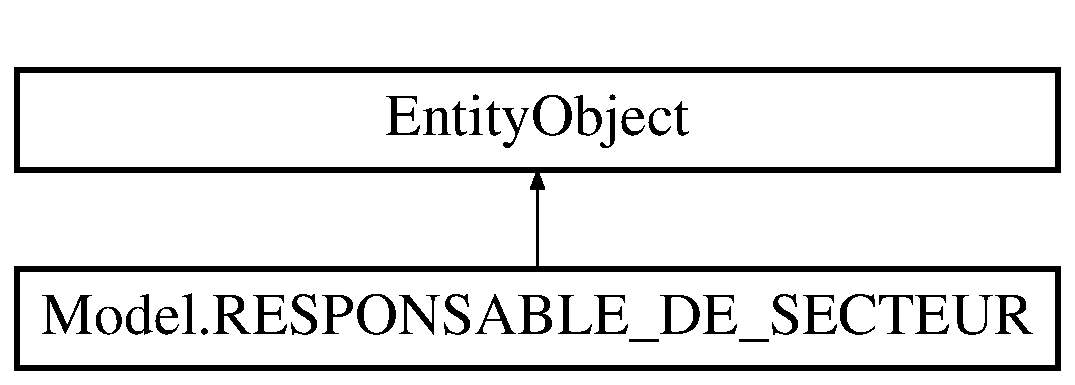
\includegraphics[height=2.000000cm]{class_model_1_1_r_e_s_p_o_n_s_a_b_l_e___d_e___s_e_c_t_e_u_r}
\end{center}
\end{figure}
\subsection*{Static Public Member Functions}
\begin{DoxyCompactItemize}
\item 
static \hyperlink{class_model_1_1_r_e_s_p_o_n_s_a_b_l_e___d_e___s_e_c_t_e_u_r}{R\-E\-S\-P\-O\-N\-S\-A\-B\-L\-E\-\_\-\-D\-E\-\_\-\-S\-E\-C\-T\-E\-U\-R} \hyperlink{class_model_1_1_r_e_s_p_o_n_s_a_b_l_e___d_e___s_e_c_t_e_u_r_a3923912985db6f098b460f54562e386f}{Create\-R\-E\-S\-P\-O\-N\-S\-A\-B\-L\-E\-\_\-\-D\-E\-\_\-\-S\-E\-C\-T\-E\-U\-R} (global\-::\-System.\-Int32 \hyperlink{class_model_1_1_r_e_s_p_o_n_s_a_b_l_e___d_e___s_e_c_t_e_u_r_af326e57ab9a6b071e90fdc7397891569}{matricule\-\_\-col\-\_\-res})
\begin{DoxyCompactList}\small\item\em Créez un nouvel objet \hyperlink{class_model_1_1_r_e_s_p_o_n_s_a_b_l_e___d_e___s_e_c_t_e_u_r}{R\-E\-S\-P\-O\-N\-S\-A\-B\-L\-E\-\_\-\-D\-E\-\_\-\-S\-E\-C\-T\-E\-U\-R}. \end{DoxyCompactList}\end{DoxyCompactItemize}
\subsection*{Properties}
\begin{DoxyCompactItemize}
\item 
global\-::\-System.\-Int32 \hyperlink{class_model_1_1_r_e_s_p_o_n_s_a_b_l_e___d_e___s_e_c_t_e_u_r_af326e57ab9a6b071e90fdc7397891569}{matricule\-\_\-col\-\_\-res}\hspace{0.3cm}{\ttfamily  \mbox{[}get, set\mbox{]}}
\begin{DoxyCompactList}\small\item\em Aucune documentation sur les métadonnées n'est disponible. \end{DoxyCompactList}\item 
\hyperlink{class_model_1_1_c_o_l_l_a_b_o_r_a_t_e_u_r}{C\-O\-L\-L\-A\-B\-O\-R\-A\-T\-E\-U\-R} \hyperlink{class_model_1_1_r_e_s_p_o_n_s_a_b_l_e___d_e___s_e_c_t_e_u_r_aff60e5a39706f59b8f1638b093db3063}{C\-O\-L\-L\-A\-B\-O\-R\-A\-T\-E\-U\-R}\hspace{0.3cm}{\ttfamily  \mbox{[}get, set\mbox{]}}
\begin{DoxyCompactList}\small\item\em Aucune documentation sur les métadonnées n'est disponible. \end{DoxyCompactList}\item 
Entity\-Reference$<$ \hyperlink{class_model_1_1_c_o_l_l_a_b_o_r_a_t_e_u_r}{C\-O\-L\-L\-A\-B\-O\-R\-A\-T\-E\-U\-R} $>$ \hyperlink{class_model_1_1_r_e_s_p_o_n_s_a_b_l_e___d_e___s_e_c_t_e_u_r_ad59165995faa8ea9fbffe4748f438090}{C\-O\-L\-L\-A\-B\-O\-R\-A\-T\-E\-U\-R\-Reference}\hspace{0.3cm}{\ttfamily  \mbox{[}get, set\mbox{]}}
\begin{DoxyCompactList}\small\item\em Aucune documentation sur les métadonnées n'est disponible. \end{DoxyCompactList}\end{DoxyCompactItemize}


\subsection{Detailed Description}
Aucune documentation sur les métadonnées n'est disponible. 



\subsection{Member Function Documentation}
\hypertarget{class_model_1_1_r_e_s_p_o_n_s_a_b_l_e___d_e___s_e_c_t_e_u_r_a3923912985db6f098b460f54562e386f}{\index{Model\-::\-R\-E\-S\-P\-O\-N\-S\-A\-B\-L\-E\-\_\-\-D\-E\-\_\-\-S\-E\-C\-T\-E\-U\-R@{Model\-::\-R\-E\-S\-P\-O\-N\-S\-A\-B\-L\-E\-\_\-\-D\-E\-\_\-\-S\-E\-C\-T\-E\-U\-R}!Create\-R\-E\-S\-P\-O\-N\-S\-A\-B\-L\-E\-\_\-\-D\-E\-\_\-\-S\-E\-C\-T\-E\-U\-R@{Create\-R\-E\-S\-P\-O\-N\-S\-A\-B\-L\-E\-\_\-\-D\-E\-\_\-\-S\-E\-C\-T\-E\-U\-R}}
\index{Create\-R\-E\-S\-P\-O\-N\-S\-A\-B\-L\-E\-\_\-\-D\-E\-\_\-\-S\-E\-C\-T\-E\-U\-R@{Create\-R\-E\-S\-P\-O\-N\-S\-A\-B\-L\-E\-\_\-\-D\-E\-\_\-\-S\-E\-C\-T\-E\-U\-R}!Model::RESPONSABLE_DE_SECTEUR@{Model\-::\-R\-E\-S\-P\-O\-N\-S\-A\-B\-L\-E\-\_\-\-D\-E\-\_\-\-S\-E\-C\-T\-E\-U\-R}}
\subsubsection[{Create\-R\-E\-S\-P\-O\-N\-S\-A\-B\-L\-E\-\_\-\-D\-E\-\_\-\-S\-E\-C\-T\-E\-U\-R}]{\setlength{\rightskip}{0pt plus 5cm}static {\bf R\-E\-S\-P\-O\-N\-S\-A\-B\-L\-E\-\_\-\-D\-E\-\_\-\-S\-E\-C\-T\-E\-U\-R} Model.\-R\-E\-S\-P\-O\-N\-S\-A\-B\-L\-E\-\_\-\-D\-E\-\_\-\-S\-E\-C\-T\-E\-U\-R.\-Create\-R\-E\-S\-P\-O\-N\-S\-A\-B\-L\-E\-\_\-\-D\-E\-\_\-\-S\-E\-C\-T\-E\-U\-R (
\begin{DoxyParamCaption}
\item[{global\-::\-System.\-Int32}]{matricule\-\_\-col\-\_\-res}
\end{DoxyParamCaption}
)\hspace{0.3cm}{\ttfamily [static]}}}\label{class_model_1_1_r_e_s_p_o_n_s_a_b_l_e___d_e___s_e_c_t_e_u_r_a3923912985db6f098b460f54562e386f}


Créez un nouvel objet \hyperlink{class_model_1_1_r_e_s_p_o_n_s_a_b_l_e___d_e___s_e_c_t_e_u_r}{R\-E\-S\-P\-O\-N\-S\-A\-B\-L\-E\-\_\-\-D\-E\-\_\-\-S\-E\-C\-T\-E\-U\-R}. 


\begin{DoxyParams}{Parameters}
{\em matricule\-\_\-col\-\_\-res} & Valeur initiale de la propriété matricule\-\_\-col\-\_\-res.\\
\hline
\end{DoxyParams}


\subsection{Property Documentation}
\hypertarget{class_model_1_1_r_e_s_p_o_n_s_a_b_l_e___d_e___s_e_c_t_e_u_r_aff60e5a39706f59b8f1638b093db3063}{\index{Model\-::\-R\-E\-S\-P\-O\-N\-S\-A\-B\-L\-E\-\_\-\-D\-E\-\_\-\-S\-E\-C\-T\-E\-U\-R@{Model\-::\-R\-E\-S\-P\-O\-N\-S\-A\-B\-L\-E\-\_\-\-D\-E\-\_\-\-S\-E\-C\-T\-E\-U\-R}!C\-O\-L\-L\-A\-B\-O\-R\-A\-T\-E\-U\-R@{C\-O\-L\-L\-A\-B\-O\-R\-A\-T\-E\-U\-R}}
\index{C\-O\-L\-L\-A\-B\-O\-R\-A\-T\-E\-U\-R@{C\-O\-L\-L\-A\-B\-O\-R\-A\-T\-E\-U\-R}!Model::RESPONSABLE_DE_SECTEUR@{Model\-::\-R\-E\-S\-P\-O\-N\-S\-A\-B\-L\-E\-\_\-\-D\-E\-\_\-\-S\-E\-C\-T\-E\-U\-R}}
\subsubsection[{C\-O\-L\-L\-A\-B\-O\-R\-A\-T\-E\-U\-R}]{\setlength{\rightskip}{0pt plus 5cm}{\bf C\-O\-L\-L\-A\-B\-O\-R\-A\-T\-E\-U\-R} Model.\-R\-E\-S\-P\-O\-N\-S\-A\-B\-L\-E\-\_\-\-D\-E\-\_\-\-S\-E\-C\-T\-E\-U\-R.\-C\-O\-L\-L\-A\-B\-O\-R\-A\-T\-E\-U\-R\hspace{0.3cm}{\ttfamily [get]}, {\ttfamily [set]}}}\label{class_model_1_1_r_e_s_p_o_n_s_a_b_l_e___d_e___s_e_c_t_e_u_r_aff60e5a39706f59b8f1638b093db3063}


Aucune documentation sur les métadonnées n'est disponible. 

\hypertarget{class_model_1_1_r_e_s_p_o_n_s_a_b_l_e___d_e___s_e_c_t_e_u_r_ad59165995faa8ea9fbffe4748f438090}{\index{Model\-::\-R\-E\-S\-P\-O\-N\-S\-A\-B\-L\-E\-\_\-\-D\-E\-\_\-\-S\-E\-C\-T\-E\-U\-R@{Model\-::\-R\-E\-S\-P\-O\-N\-S\-A\-B\-L\-E\-\_\-\-D\-E\-\_\-\-S\-E\-C\-T\-E\-U\-R}!C\-O\-L\-L\-A\-B\-O\-R\-A\-T\-E\-U\-R\-Reference@{C\-O\-L\-L\-A\-B\-O\-R\-A\-T\-E\-U\-R\-Reference}}
\index{C\-O\-L\-L\-A\-B\-O\-R\-A\-T\-E\-U\-R\-Reference@{C\-O\-L\-L\-A\-B\-O\-R\-A\-T\-E\-U\-R\-Reference}!Model::RESPONSABLE_DE_SECTEUR@{Model\-::\-R\-E\-S\-P\-O\-N\-S\-A\-B\-L\-E\-\_\-\-D\-E\-\_\-\-S\-E\-C\-T\-E\-U\-R}}
\subsubsection[{C\-O\-L\-L\-A\-B\-O\-R\-A\-T\-E\-U\-R\-Reference}]{\setlength{\rightskip}{0pt plus 5cm}Entity\-Reference$<${\bf C\-O\-L\-L\-A\-B\-O\-R\-A\-T\-E\-U\-R}$>$ Model.\-R\-E\-S\-P\-O\-N\-S\-A\-B\-L\-E\-\_\-\-D\-E\-\_\-\-S\-E\-C\-T\-E\-U\-R.\-C\-O\-L\-L\-A\-B\-O\-R\-A\-T\-E\-U\-R\-Reference\hspace{0.3cm}{\ttfamily [get]}, {\ttfamily [set]}}}\label{class_model_1_1_r_e_s_p_o_n_s_a_b_l_e___d_e___s_e_c_t_e_u_r_ad59165995faa8ea9fbffe4748f438090}


Aucune documentation sur les métadonnées n'est disponible. 

\hypertarget{class_model_1_1_r_e_s_p_o_n_s_a_b_l_e___d_e___s_e_c_t_e_u_r_af326e57ab9a6b071e90fdc7397891569}{\index{Model\-::\-R\-E\-S\-P\-O\-N\-S\-A\-B\-L\-E\-\_\-\-D\-E\-\_\-\-S\-E\-C\-T\-E\-U\-R@{Model\-::\-R\-E\-S\-P\-O\-N\-S\-A\-B\-L\-E\-\_\-\-D\-E\-\_\-\-S\-E\-C\-T\-E\-U\-R}!matricule\-\_\-col\-\_\-res@{matricule\-\_\-col\-\_\-res}}
\index{matricule\-\_\-col\-\_\-res@{matricule\-\_\-col\-\_\-res}!Model::RESPONSABLE_DE_SECTEUR@{Model\-::\-R\-E\-S\-P\-O\-N\-S\-A\-B\-L\-E\-\_\-\-D\-E\-\_\-\-S\-E\-C\-T\-E\-U\-R}}
\subsubsection[{matricule\-\_\-col\-\_\-res}]{\setlength{\rightskip}{0pt plus 5cm}global.\-System.\-Int32 Model.\-R\-E\-S\-P\-O\-N\-S\-A\-B\-L\-E\-\_\-\-D\-E\-\_\-\-S\-E\-C\-T\-E\-U\-R.\-matricule\-\_\-col\-\_\-res\hspace{0.3cm}{\ttfamily [get]}, {\ttfamily [set]}}}\label{class_model_1_1_r_e_s_p_o_n_s_a_b_l_e___d_e___s_e_c_t_e_u_r_af326e57ab9a6b071e90fdc7397891569}


Aucune documentation sur les métadonnées n'est disponible. 



The documentation for this class was generated from the following file\-:\begin{DoxyCompactItemize}
\item 
C\-:/\-Users/dju/\-Documents/\-Visual Studio 2012/\-Projects/\-P\-P\-E/\-P\-P\-E3/\-Model/\hyperlink{_model_bdd_sio_8_designer_8cs}{Model\-Bdd\-Sio.\-Designer.\-cs}\end{DoxyCompactItemize}

\hypertarget{class_model_1_1_s_e_c_t_e_u_r}{\section{Model.\-S\-E\-C\-T\-E\-U\-R Class Reference}
\label{class_model_1_1_s_e_c_t_e_u_r}\index{Model.\-S\-E\-C\-T\-E\-U\-R@{Model.\-S\-E\-C\-T\-E\-U\-R}}
}


Aucune documentation sur les métadonnées n'est disponible.  


Inheritance diagram for Model.\-S\-E\-C\-T\-E\-U\-R\-:\begin{figure}[H]
\begin{center}
\leavevmode
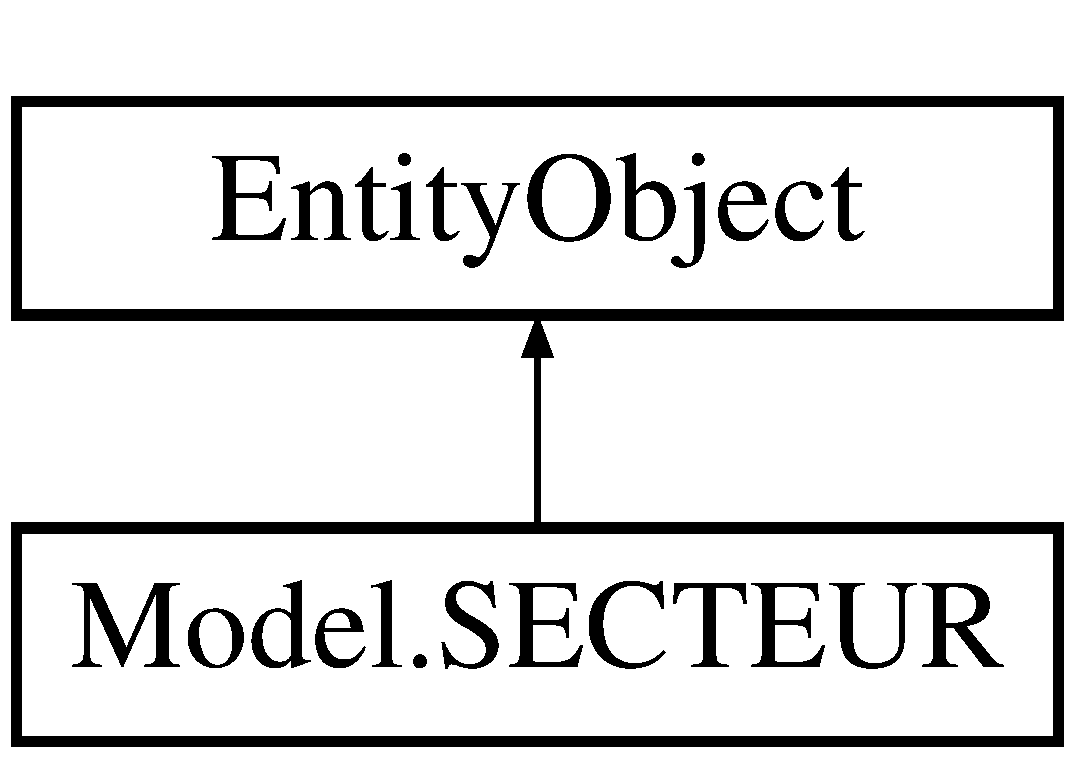
\includegraphics[height=2.000000cm]{class_model_1_1_s_e_c_t_e_u_r}
\end{center}
\end{figure}
\subsection*{Static Public Member Functions}
\begin{DoxyCompactItemize}
\item 
static \hyperlink{class_model_1_1_s_e_c_t_e_u_r}{S\-E\-C\-T\-E\-U\-R} \hyperlink{class_model_1_1_s_e_c_t_e_u_r_a05f46909f4d42aa7093230a5bec5c6b4}{Create\-S\-E\-C\-T\-E\-U\-R} (global\-::\-System.\-String \hyperlink{class_model_1_1_s_e_c_t_e_u_r_a08444aca8045d7e1ce29ad2d8760807d}{code\-\_\-secteur}, global\-::\-System.\-String \hyperlink{class_model_1_1_s_e_c_t_e_u_r_acd43f9e6cd67fd6018645b7c944fcf40}{libelle\-\_\-secteur})
\begin{DoxyCompactList}\small\item\em Créez un nouvel objet \hyperlink{class_model_1_1_s_e_c_t_e_u_r}{S\-E\-C\-T\-E\-U\-R}. \end{DoxyCompactList}\end{DoxyCompactItemize}
\subsection*{Properties}
\begin{DoxyCompactItemize}
\item 
global\-::\-System.\-String \hyperlink{class_model_1_1_s_e_c_t_e_u_r_a08444aca8045d7e1ce29ad2d8760807d}{code\-\_\-secteur}\hspace{0.3cm}{\ttfamily  \mbox{[}get, set\mbox{]}}
\begin{DoxyCompactList}\small\item\em Aucune documentation sur les métadonnées n'est disponible. \end{DoxyCompactList}\item 
global\-::\-System.\-String \hyperlink{class_model_1_1_s_e_c_t_e_u_r_acd43f9e6cd67fd6018645b7c944fcf40}{libelle\-\_\-secteur}\hspace{0.3cm}{\ttfamily  \mbox{[}get, set\mbox{]}}
\begin{DoxyCompactList}\small\item\em Aucune documentation sur les métadonnées n'est disponible. \end{DoxyCompactList}\item 
Entity\-Collection\\*
$<$ \hyperlink{class_model_1_1_e_t_r_e___r_e_s_p_o_n_s_a_b_l_e}{E\-T\-R\-E\-\_\-\-R\-E\-S\-P\-O\-N\-S\-A\-B\-L\-E} $>$ \hyperlink{class_model_1_1_s_e_c_t_e_u_r_a6ae4e9f4e0e89e1fe68995194972a6db}{E\-T\-R\-E\-\_\-\-R\-E\-S\-P\-O\-N\-S\-A\-B\-L\-E}\hspace{0.3cm}{\ttfamily  \mbox{[}get, set\mbox{]}}
\begin{DoxyCompactList}\small\item\em Aucune documentation sur les métadonnées n'est disponible. \end{DoxyCompactList}\item 
Entity\-Collection$<$ \hyperlink{class_model_1_1_r_e_g_i_o_n}{R\-E\-G\-I\-O\-N} $>$ \hyperlink{class_model_1_1_s_e_c_t_e_u_r_a10eb57d7aa180eb2757990d77002b00e}{R\-E\-G\-I\-O\-N}\hspace{0.3cm}{\ttfamily  \mbox{[}get, set\mbox{]}}
\begin{DoxyCompactList}\small\item\em Aucune documentation sur les métadonnées n'est disponible. \end{DoxyCompactList}\end{DoxyCompactItemize}


\subsection{Detailed Description}
Aucune documentation sur les métadonnées n'est disponible. 



\subsection{Member Function Documentation}
\hypertarget{class_model_1_1_s_e_c_t_e_u_r_a05f46909f4d42aa7093230a5bec5c6b4}{\index{Model\-::\-S\-E\-C\-T\-E\-U\-R@{Model\-::\-S\-E\-C\-T\-E\-U\-R}!Create\-S\-E\-C\-T\-E\-U\-R@{Create\-S\-E\-C\-T\-E\-U\-R}}
\index{Create\-S\-E\-C\-T\-E\-U\-R@{Create\-S\-E\-C\-T\-E\-U\-R}!Model::SECTEUR@{Model\-::\-S\-E\-C\-T\-E\-U\-R}}
\subsubsection[{Create\-S\-E\-C\-T\-E\-U\-R}]{\setlength{\rightskip}{0pt plus 5cm}static {\bf S\-E\-C\-T\-E\-U\-R} Model.\-S\-E\-C\-T\-E\-U\-R.\-Create\-S\-E\-C\-T\-E\-U\-R (
\begin{DoxyParamCaption}
\item[{global\-::\-System.\-String}]{code\-\_\-secteur, }
\item[{global\-::\-System.\-String}]{libelle\-\_\-secteur}
\end{DoxyParamCaption}
)\hspace{0.3cm}{\ttfamily [static]}}}\label{class_model_1_1_s_e_c_t_e_u_r_a05f46909f4d42aa7093230a5bec5c6b4}


Créez un nouvel objet \hyperlink{class_model_1_1_s_e_c_t_e_u_r}{S\-E\-C\-T\-E\-U\-R}. 


\begin{DoxyParams}{Parameters}
{\em code\-\_\-secteur} & Valeur initiale de la propriété code\-\_\-secteur.\\
\hline
{\em libelle\-\_\-secteur} & Valeur initiale de la propriété libelle\-\_\-secteur.\\
\hline
\end{DoxyParams}


\subsection{Property Documentation}
\hypertarget{class_model_1_1_s_e_c_t_e_u_r_a08444aca8045d7e1ce29ad2d8760807d}{\index{Model\-::\-S\-E\-C\-T\-E\-U\-R@{Model\-::\-S\-E\-C\-T\-E\-U\-R}!code\-\_\-secteur@{code\-\_\-secteur}}
\index{code\-\_\-secteur@{code\-\_\-secteur}!Model::SECTEUR@{Model\-::\-S\-E\-C\-T\-E\-U\-R}}
\subsubsection[{code\-\_\-secteur}]{\setlength{\rightskip}{0pt plus 5cm}global.\-System.\-String Model.\-S\-E\-C\-T\-E\-U\-R.\-code\-\_\-secteur\hspace{0.3cm}{\ttfamily [get]}, {\ttfamily [set]}}}\label{class_model_1_1_s_e_c_t_e_u_r_a08444aca8045d7e1ce29ad2d8760807d}


Aucune documentation sur les métadonnées n'est disponible. 

\hypertarget{class_model_1_1_s_e_c_t_e_u_r_a6ae4e9f4e0e89e1fe68995194972a6db}{\index{Model\-::\-S\-E\-C\-T\-E\-U\-R@{Model\-::\-S\-E\-C\-T\-E\-U\-R}!E\-T\-R\-E\-\_\-\-R\-E\-S\-P\-O\-N\-S\-A\-B\-L\-E@{E\-T\-R\-E\-\_\-\-R\-E\-S\-P\-O\-N\-S\-A\-B\-L\-E}}
\index{E\-T\-R\-E\-\_\-\-R\-E\-S\-P\-O\-N\-S\-A\-B\-L\-E@{E\-T\-R\-E\-\_\-\-R\-E\-S\-P\-O\-N\-S\-A\-B\-L\-E}!Model::SECTEUR@{Model\-::\-S\-E\-C\-T\-E\-U\-R}}
\subsubsection[{E\-T\-R\-E\-\_\-\-R\-E\-S\-P\-O\-N\-S\-A\-B\-L\-E}]{\setlength{\rightskip}{0pt plus 5cm}Entity\-Collection$<${\bf E\-T\-R\-E\-\_\-\-R\-E\-S\-P\-O\-N\-S\-A\-B\-L\-E}$>$ Model.\-S\-E\-C\-T\-E\-U\-R.\-E\-T\-R\-E\-\_\-\-R\-E\-S\-P\-O\-N\-S\-A\-B\-L\-E\hspace{0.3cm}{\ttfamily [get]}, {\ttfamily [set]}}}\label{class_model_1_1_s_e_c_t_e_u_r_a6ae4e9f4e0e89e1fe68995194972a6db}


Aucune documentation sur les métadonnées n'est disponible. 

\hypertarget{class_model_1_1_s_e_c_t_e_u_r_acd43f9e6cd67fd6018645b7c944fcf40}{\index{Model\-::\-S\-E\-C\-T\-E\-U\-R@{Model\-::\-S\-E\-C\-T\-E\-U\-R}!libelle\-\_\-secteur@{libelle\-\_\-secteur}}
\index{libelle\-\_\-secteur@{libelle\-\_\-secteur}!Model::SECTEUR@{Model\-::\-S\-E\-C\-T\-E\-U\-R}}
\subsubsection[{libelle\-\_\-secteur}]{\setlength{\rightskip}{0pt plus 5cm}global.\-System.\-String Model.\-S\-E\-C\-T\-E\-U\-R.\-libelle\-\_\-secteur\hspace{0.3cm}{\ttfamily [get]}, {\ttfamily [set]}}}\label{class_model_1_1_s_e_c_t_e_u_r_acd43f9e6cd67fd6018645b7c944fcf40}


Aucune documentation sur les métadonnées n'est disponible. 

\hypertarget{class_model_1_1_s_e_c_t_e_u_r_a10eb57d7aa180eb2757990d77002b00e}{\index{Model\-::\-S\-E\-C\-T\-E\-U\-R@{Model\-::\-S\-E\-C\-T\-E\-U\-R}!R\-E\-G\-I\-O\-N@{R\-E\-G\-I\-O\-N}}
\index{R\-E\-G\-I\-O\-N@{R\-E\-G\-I\-O\-N}!Model::SECTEUR@{Model\-::\-S\-E\-C\-T\-E\-U\-R}}
\subsubsection[{R\-E\-G\-I\-O\-N}]{\setlength{\rightskip}{0pt plus 5cm}Entity\-Collection$<${\bf R\-E\-G\-I\-O\-N}$>$ Model.\-S\-E\-C\-T\-E\-U\-R.\-R\-E\-G\-I\-O\-N\hspace{0.3cm}{\ttfamily [get]}, {\ttfamily [set]}}}\label{class_model_1_1_s_e_c_t_e_u_r_a10eb57d7aa180eb2757990d77002b00e}


Aucune documentation sur les métadonnées n'est disponible. 



The documentation for this class was generated from the following file\-:\begin{DoxyCompactItemize}
\item 
C\-:/\-Users/dju/\-Documents/\-Visual Studio 2012/\-Projects/\-P\-P\-E/\-P\-P\-E3/\-Model/\hyperlink{_model_bdd_sio_8_designer_8cs}{Model\-Bdd\-Sio.\-Designer.\-cs}\end{DoxyCompactItemize}

\hypertarget{class_model_1_1_service_bdd}{\section{Model.\-Service\-Bdd Class Reference}
\label{class_model_1_1_service_bdd}\index{Model.\-Service\-Bdd@{Model.\-Service\-Bdd}}
}
Inheritance diagram for Model.\-Service\-Bdd\-:\begin{figure}[H]
\begin{center}
\leavevmode
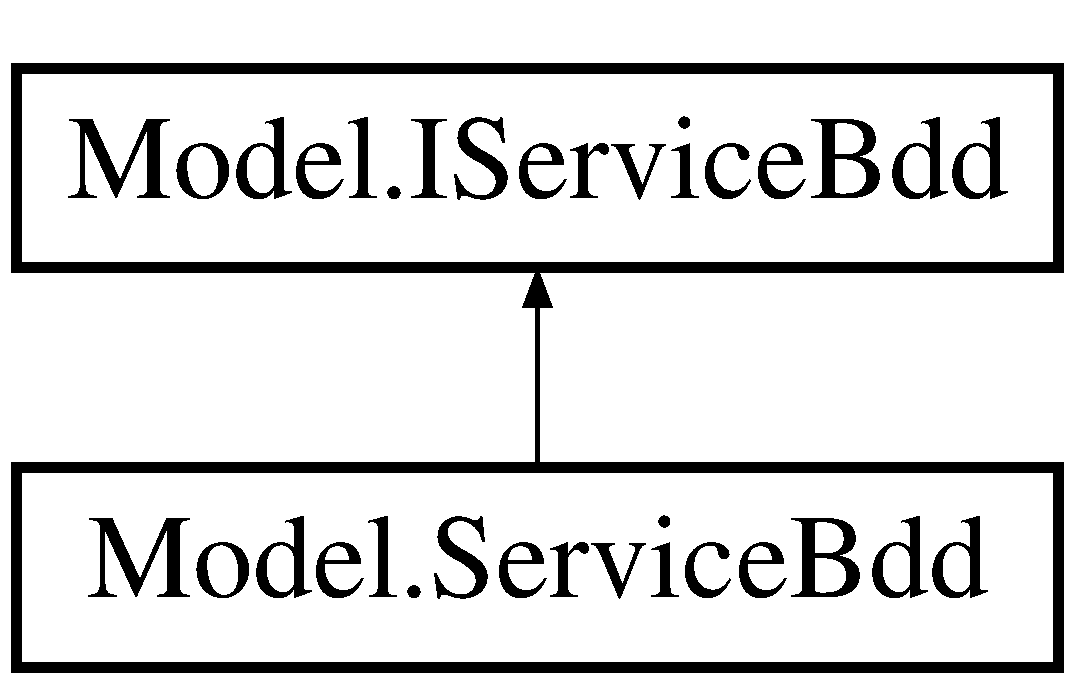
\includegraphics[height=2.000000cm]{class_model_1_1_service_bdd}
\end{center}
\end{figure}


The documentation for this class was generated from the following file\-:\begin{DoxyCompactItemize}
\item 
C\-:/\-Users/dju/\-Documents/\-Visual Studio 2012/\-Projects/\-P\-P\-E/\-P\-P\-E3/\-Model/\hyperlink{_service_bdd_8cs}{Service\-Bdd.\-cs}\end{DoxyCompactItemize}

\hypertarget{class_wpf_application_1_1_model_1_1_service_client}{\section{Wpf\-Application.\-Model.\-Service\-Client Class Reference}
\label{class_wpf_application_1_1_model_1_1_service_client}\index{Wpf\-Application.\-Model.\-Service\-Client@{Wpf\-Application.\-Model.\-Service\-Client}}
}
Inheritance diagram for Wpf\-Application.\-Model.\-Service\-Client\-:\begin{figure}[H]
\begin{center}
\leavevmode
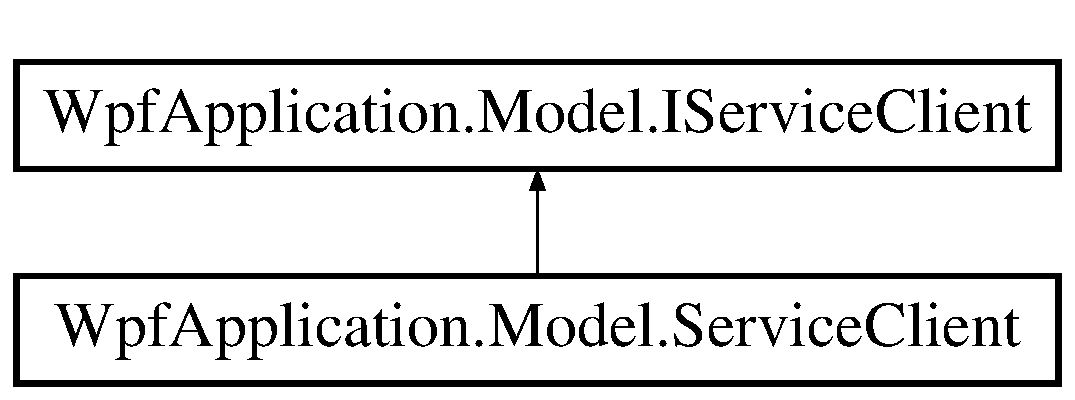
\includegraphics[height=2.000000cm]{class_wpf_application_1_1_model_1_1_service_client}
\end{center}
\end{figure}
\subsection*{Public Member Functions}
\begin{DoxyCompactItemize}
\item 
\hyperlink{class_wpf_application_1_1_model_1_1_client}{Client} \hyperlink{class_wpf_application_1_1_model_1_1_service_client_aa018b0dfc38292ba0e1bf41715914d12}{Charger} ()
\item 
List$<$ \hyperlink{class_wpf_application_1_1_model_1_1_client}{Client} $>$ \hyperlink{class_wpf_application_1_1_model_1_1_service_client_ac0b022539676651b790b38762026f0f1}{Charger\-Tout} ()
\end{DoxyCompactItemize}


\subsection{Member Function Documentation}
\hypertarget{class_wpf_application_1_1_model_1_1_service_client_aa018b0dfc38292ba0e1bf41715914d12}{\index{Wpf\-Application\-::\-Model\-::\-Service\-Client@{Wpf\-Application\-::\-Model\-::\-Service\-Client}!Charger@{Charger}}
\index{Charger@{Charger}!WpfApplication::Model::ServiceClient@{Wpf\-Application\-::\-Model\-::\-Service\-Client}}
\subsubsection[{Charger}]{\setlength{\rightskip}{0pt plus 5cm}{\bf Client} Wpf\-Application.\-Model.\-Service\-Client.\-Charger (
\begin{DoxyParamCaption}
{}
\end{DoxyParamCaption}
)}}\label{class_wpf_application_1_1_model_1_1_service_client_aa018b0dfc38292ba0e1bf41715914d12}


Implements \hyperlink{interface_wpf_application_1_1_model_1_1_i_service_client_ab513b6cf91c0d31cfe37004ac5cf7e1e}{Wpf\-Application.\-Model.\-I\-Service\-Client}.

\hypertarget{class_wpf_application_1_1_model_1_1_service_client_ac0b022539676651b790b38762026f0f1}{\index{Wpf\-Application\-::\-Model\-::\-Service\-Client@{Wpf\-Application\-::\-Model\-::\-Service\-Client}!Charger\-Tout@{Charger\-Tout}}
\index{Charger\-Tout@{Charger\-Tout}!WpfApplication::Model::ServiceClient@{Wpf\-Application\-::\-Model\-::\-Service\-Client}}
\subsubsection[{Charger\-Tout}]{\setlength{\rightskip}{0pt plus 5cm}List$<${\bf Client}$>$ Wpf\-Application.\-Model.\-Service\-Client.\-Charger\-Tout (
\begin{DoxyParamCaption}
{}
\end{DoxyParamCaption}
)}}\label{class_wpf_application_1_1_model_1_1_service_client_ac0b022539676651b790b38762026f0f1}


Implements \hyperlink{interface_wpf_application_1_1_model_1_1_i_service_client_a40ae24e7195bb27667e26ed27319c3e5}{Wpf\-Application.\-Model.\-I\-Service\-Client}.



The documentation for this class was generated from the following file\-:\begin{DoxyCompactItemize}
\item 
C\-:/\-Users/dju/\-Documents/\-Visual Studio 2012/\-Projects/\-P\-P\-E/\-P\-P\-E3/\-Wpf\-Application/\-Model/\hyperlink{_service_client_8cs}{Service\-Client.\-cs}\end{DoxyCompactItemize}

\hypertarget{class_model_1_1_s_p_e_c_i_a_l_i_t_e}{\section{Model.\-S\-P\-E\-C\-I\-A\-L\-I\-T\-E Class Reference}
\label{class_model_1_1_s_p_e_c_i_a_l_i_t_e}\index{Model.\-S\-P\-E\-C\-I\-A\-L\-I\-T\-E@{Model.\-S\-P\-E\-C\-I\-A\-L\-I\-T\-E}}
}


Aucune documentation sur les métadonnées n'est disponible.  


Inheritance diagram for Model.\-S\-P\-E\-C\-I\-A\-L\-I\-T\-E\-:\begin{figure}[H]
\begin{center}
\leavevmode
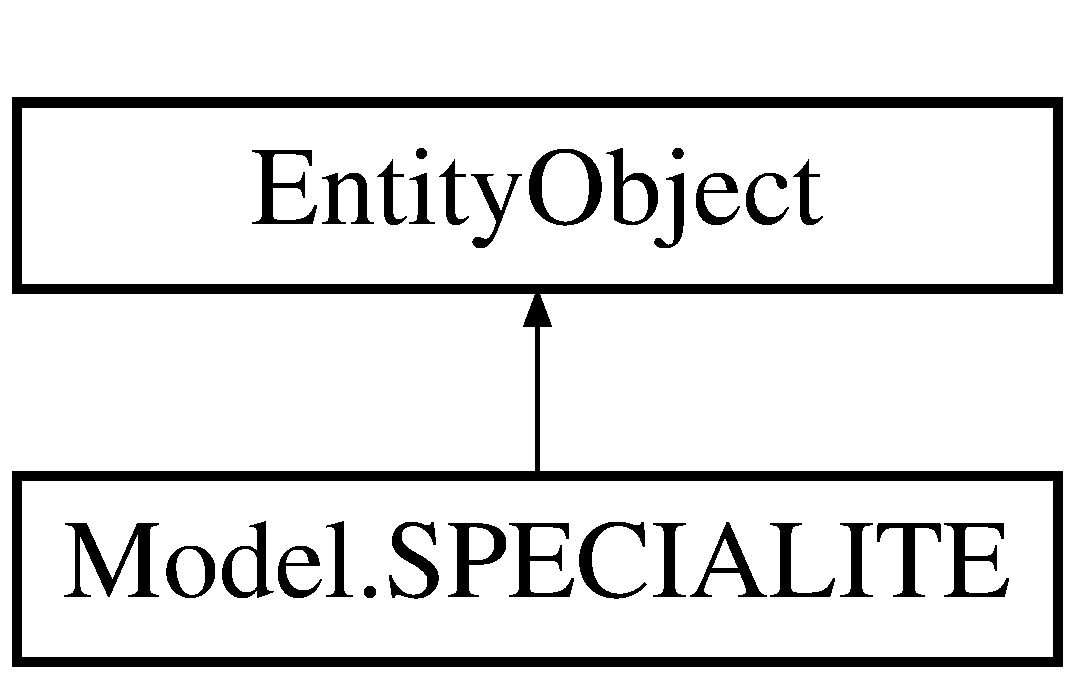
\includegraphics[height=2.000000cm]{class_model_1_1_s_p_e_c_i_a_l_i_t_e}
\end{center}
\end{figure}
\subsection*{Static Public Member Functions}
\begin{DoxyCompactItemize}
\item 
static \hyperlink{class_model_1_1_s_p_e_c_i_a_l_i_t_e}{S\-P\-E\-C\-I\-A\-L\-I\-T\-E} \hyperlink{class_model_1_1_s_p_e_c_i_a_l_i_t_e_ac40ba96bb21c40f9df63224799ad63cd}{Create\-S\-P\-E\-C\-I\-A\-L\-I\-T\-E} (global\-::\-System.\-Int32 \hyperlink{class_model_1_1_s_p_e_c_i_a_l_i_t_e_a3f2f2a136e0e517600c23a5ebb9d9cac}{code\-\_\-spec}, global\-::\-System.\-String \hyperlink{class_model_1_1_s_p_e_c_i_a_l_i_t_e_a82916a9c724d347181c4e30fba74c3ff}{libelle\-\_\-spec})
\begin{DoxyCompactList}\small\item\em Créez un nouvel objet \hyperlink{class_model_1_1_s_p_e_c_i_a_l_i_t_e}{S\-P\-E\-C\-I\-A\-L\-I\-T\-E}. \end{DoxyCompactList}\end{DoxyCompactItemize}
\subsection*{Properties}
\begin{DoxyCompactItemize}
\item 
global\-::\-System.\-Int32 \hyperlink{class_model_1_1_s_p_e_c_i_a_l_i_t_e_a3f2f2a136e0e517600c23a5ebb9d9cac}{code\-\_\-spec}\hspace{0.3cm}{\ttfamily  \mbox{[}get, set\mbox{]}}
\begin{DoxyCompactList}\small\item\em Aucune documentation sur les métadonnées n'est disponible. \end{DoxyCompactList}\item 
global\-::\-System.\-String \hyperlink{class_model_1_1_s_p_e_c_i_a_l_i_t_e_a82916a9c724d347181c4e30fba74c3ff}{libelle\-\_\-spec}\hspace{0.3cm}{\ttfamily  \mbox{[}get, set\mbox{]}}
\begin{DoxyCompactList}\small\item\em Aucune documentation sur les métadonnées n'est disponible. \end{DoxyCompactList}\item 
Entity\-Collection$<$ \hyperlink{class_model_1_1_p_r_a_t_i_c_i_e_n}{P\-R\-A\-T\-I\-C\-I\-E\-N} $>$ \hyperlink{class_model_1_1_s_p_e_c_i_a_l_i_t_e_ab96edcc3579c95087e878fdeff929e00}{P\-R\-A\-T\-I\-C\-I\-E\-N}\hspace{0.3cm}{\ttfamily  \mbox{[}get, set\mbox{]}}
\begin{DoxyCompactList}\small\item\em Aucune documentation sur les métadonnées n'est disponible. \end{DoxyCompactList}\end{DoxyCompactItemize}


\subsection{Detailed Description}
Aucune documentation sur les métadonnées n'est disponible. 



\subsection{Member Function Documentation}
\hypertarget{class_model_1_1_s_p_e_c_i_a_l_i_t_e_ac40ba96bb21c40f9df63224799ad63cd}{\index{Model\-::\-S\-P\-E\-C\-I\-A\-L\-I\-T\-E@{Model\-::\-S\-P\-E\-C\-I\-A\-L\-I\-T\-E}!Create\-S\-P\-E\-C\-I\-A\-L\-I\-T\-E@{Create\-S\-P\-E\-C\-I\-A\-L\-I\-T\-E}}
\index{Create\-S\-P\-E\-C\-I\-A\-L\-I\-T\-E@{Create\-S\-P\-E\-C\-I\-A\-L\-I\-T\-E}!Model::SPECIALITE@{Model\-::\-S\-P\-E\-C\-I\-A\-L\-I\-T\-E}}
\subsubsection[{Create\-S\-P\-E\-C\-I\-A\-L\-I\-T\-E}]{\setlength{\rightskip}{0pt plus 5cm}static {\bf S\-P\-E\-C\-I\-A\-L\-I\-T\-E} Model.\-S\-P\-E\-C\-I\-A\-L\-I\-T\-E.\-Create\-S\-P\-E\-C\-I\-A\-L\-I\-T\-E (
\begin{DoxyParamCaption}
\item[{global\-::\-System.\-Int32}]{code\-\_\-spec, }
\item[{global\-::\-System.\-String}]{libelle\-\_\-spec}
\end{DoxyParamCaption}
)\hspace{0.3cm}{\ttfamily [static]}}}\label{class_model_1_1_s_p_e_c_i_a_l_i_t_e_ac40ba96bb21c40f9df63224799ad63cd}


Créez un nouvel objet \hyperlink{class_model_1_1_s_p_e_c_i_a_l_i_t_e}{S\-P\-E\-C\-I\-A\-L\-I\-T\-E}. 


\begin{DoxyParams}{Parameters}
{\em code\-\_\-spec} & Valeur initiale de la propriété code\-\_\-spec.\\
\hline
{\em libelle\-\_\-spec} & Valeur initiale de la propriété libelle\-\_\-spec.\\
\hline
\end{DoxyParams}


\subsection{Property Documentation}
\hypertarget{class_model_1_1_s_p_e_c_i_a_l_i_t_e_a3f2f2a136e0e517600c23a5ebb9d9cac}{\index{Model\-::\-S\-P\-E\-C\-I\-A\-L\-I\-T\-E@{Model\-::\-S\-P\-E\-C\-I\-A\-L\-I\-T\-E}!code\-\_\-spec@{code\-\_\-spec}}
\index{code\-\_\-spec@{code\-\_\-spec}!Model::SPECIALITE@{Model\-::\-S\-P\-E\-C\-I\-A\-L\-I\-T\-E}}
\subsubsection[{code\-\_\-spec}]{\setlength{\rightskip}{0pt plus 5cm}global.\-System.\-Int32 Model.\-S\-P\-E\-C\-I\-A\-L\-I\-T\-E.\-code\-\_\-spec\hspace{0.3cm}{\ttfamily [get]}, {\ttfamily [set]}}}\label{class_model_1_1_s_p_e_c_i_a_l_i_t_e_a3f2f2a136e0e517600c23a5ebb9d9cac}


Aucune documentation sur les métadonnées n'est disponible. 

\hypertarget{class_model_1_1_s_p_e_c_i_a_l_i_t_e_a82916a9c724d347181c4e30fba74c3ff}{\index{Model\-::\-S\-P\-E\-C\-I\-A\-L\-I\-T\-E@{Model\-::\-S\-P\-E\-C\-I\-A\-L\-I\-T\-E}!libelle\-\_\-spec@{libelle\-\_\-spec}}
\index{libelle\-\_\-spec@{libelle\-\_\-spec}!Model::SPECIALITE@{Model\-::\-S\-P\-E\-C\-I\-A\-L\-I\-T\-E}}
\subsubsection[{libelle\-\_\-spec}]{\setlength{\rightskip}{0pt plus 5cm}global.\-System.\-String Model.\-S\-P\-E\-C\-I\-A\-L\-I\-T\-E.\-libelle\-\_\-spec\hspace{0.3cm}{\ttfamily [get]}, {\ttfamily [set]}}}\label{class_model_1_1_s_p_e_c_i_a_l_i_t_e_a82916a9c724d347181c4e30fba74c3ff}


Aucune documentation sur les métadonnées n'est disponible. 

\hypertarget{class_model_1_1_s_p_e_c_i_a_l_i_t_e_ab96edcc3579c95087e878fdeff929e00}{\index{Model\-::\-S\-P\-E\-C\-I\-A\-L\-I\-T\-E@{Model\-::\-S\-P\-E\-C\-I\-A\-L\-I\-T\-E}!P\-R\-A\-T\-I\-C\-I\-E\-N@{P\-R\-A\-T\-I\-C\-I\-E\-N}}
\index{P\-R\-A\-T\-I\-C\-I\-E\-N@{P\-R\-A\-T\-I\-C\-I\-E\-N}!Model::SPECIALITE@{Model\-::\-S\-P\-E\-C\-I\-A\-L\-I\-T\-E}}
\subsubsection[{P\-R\-A\-T\-I\-C\-I\-E\-N}]{\setlength{\rightskip}{0pt plus 5cm}Entity\-Collection$<${\bf P\-R\-A\-T\-I\-C\-I\-E\-N}$>$ Model.\-S\-P\-E\-C\-I\-A\-L\-I\-T\-E.\-P\-R\-A\-T\-I\-C\-I\-E\-N\hspace{0.3cm}{\ttfamily [get]}, {\ttfamily [set]}}}\label{class_model_1_1_s_p_e_c_i_a_l_i_t_e_ab96edcc3579c95087e878fdeff929e00}


Aucune documentation sur les métadonnées n'est disponible. 



The documentation for this class was generated from the following file\-:\begin{DoxyCompactItemize}
\item 
C\-:/\-Users/dju/\-Documents/\-Visual Studio 2012/\-Projects/\-P\-P\-E/\-P\-P\-E3/\-Model/\hyperlink{_model_bdd_sio_8_designer_8cs}{Model\-Bdd\-Sio.\-Designer.\-cs}\end{DoxyCompactItemize}

\hypertarget{class_model_1_1sysdiagrams}{\section{Model.\-sysdiagrams Class Reference}
\label{class_model_1_1sysdiagrams}\index{Model.\-sysdiagrams@{Model.\-sysdiagrams}}
}


Aucune documentation sur les métadonnées n'est disponible.  


Inheritance diagram for Model.\-sysdiagrams\-:\begin{figure}[H]
\begin{center}
\leavevmode
\includegraphics[height=2.000000cm]{class_model_1_1sysdiagrams}
\end{center}
\end{figure}
\subsection*{Static Public Member Functions}
\begin{DoxyCompactItemize}
\item 
static \hyperlink{class_model_1_1sysdiagrams}{sysdiagrams} \hyperlink{class_model_1_1sysdiagrams_a0bfba4d60b5d866002878c64d33a38ff}{Createsysdiagrams} (global\-::\-System.\-String \hyperlink{class_model_1_1sysdiagrams_a7b2a5e745f15a3fde21f58e57786c2a0}{name}, global\-::\-System.\-Int32 \hyperlink{class_model_1_1sysdiagrams_ae438ae2c8f6f3fa8f1a52aeabdba5efd}{principal\-\_\-id}, global\-::\-System.\-Int32 \hyperlink{class_model_1_1sysdiagrams_a9ce7be08043952209a0b1fce62fe0d86}{diagram\-\_\-id})
\begin{DoxyCompactList}\small\item\em Créez un nouvel objet sysdiagrams. \end{DoxyCompactList}\end{DoxyCompactItemize}
\subsection*{Properties}
\begin{DoxyCompactItemize}
\item 
global\-::\-System.\-String \hyperlink{class_model_1_1sysdiagrams_a7b2a5e745f15a3fde21f58e57786c2a0}{name}\hspace{0.3cm}{\ttfamily  \mbox{[}get, set\mbox{]}}
\begin{DoxyCompactList}\small\item\em Aucune documentation sur les métadonnées n'est disponible. \end{DoxyCompactList}\item 
global\-::\-System.\-Int32 \hyperlink{class_model_1_1sysdiagrams_ae438ae2c8f6f3fa8f1a52aeabdba5efd}{principal\-\_\-id}\hspace{0.3cm}{\ttfamily  \mbox{[}get, set\mbox{]}}
\begin{DoxyCompactList}\small\item\em Aucune documentation sur les métadonnées n'est disponible. \end{DoxyCompactList}\item 
global\-::\-System.\-Int32 \hyperlink{class_model_1_1sysdiagrams_a9ce7be08043952209a0b1fce62fe0d86}{diagram\-\_\-id}\hspace{0.3cm}{\ttfamily  \mbox{[}get, set\mbox{]}}
\begin{DoxyCompactList}\small\item\em Aucune documentation sur les métadonnées n'est disponible. \end{DoxyCompactList}\item 
Nullable$<$ global\-::\-System.\-Int32 $>$ \hyperlink{class_model_1_1sysdiagrams_a173f1f695fb8a41ddbb2b1591650fd59}{version}\hspace{0.3cm}{\ttfamily  \mbox{[}get, set\mbox{]}}
\begin{DoxyCompactList}\small\item\em Aucune documentation sur les métadonnées n'est disponible. \end{DoxyCompactList}\item 
global\-::\-System.\-Byte\mbox{[}$\,$\mbox{]} \hyperlink{class_model_1_1sysdiagrams_a987f2c535acceec4fa63362005fcf726}{definition}\hspace{0.3cm}{\ttfamily  \mbox{[}get, set\mbox{]}}
\begin{DoxyCompactList}\small\item\em Aucune documentation sur les métadonnées n'est disponible. \end{DoxyCompactList}\end{DoxyCompactItemize}


\subsection{Detailed Description}
Aucune documentation sur les métadonnées n'est disponible. 



\subsection{Member Function Documentation}
\hypertarget{class_model_1_1sysdiagrams_a0bfba4d60b5d866002878c64d33a38ff}{\index{Model\-::sysdiagrams@{Model\-::sysdiagrams}!Createsysdiagrams@{Createsysdiagrams}}
\index{Createsysdiagrams@{Createsysdiagrams}!Model::sysdiagrams@{Model\-::sysdiagrams}}
\subsubsection[{Createsysdiagrams}]{\setlength{\rightskip}{0pt plus 5cm}static {\bf sysdiagrams} Model.\-sysdiagrams.\-Createsysdiagrams (
\begin{DoxyParamCaption}
\item[{global\-::\-System.\-String}]{name, }
\item[{global\-::\-System.\-Int32}]{principal\-\_\-id, }
\item[{global\-::\-System.\-Int32}]{diagram\-\_\-id}
\end{DoxyParamCaption}
)\hspace{0.3cm}{\ttfamily [static]}}}\label{class_model_1_1sysdiagrams_a0bfba4d60b5d866002878c64d33a38ff}


Créez un nouvel objet sysdiagrams. 


\begin{DoxyParams}{Parameters}
{\em name} & Valeur initiale de la propriété name.\\
\hline
{\em principal\-\_\-id} & Valeur initiale de la propriété principal\-\_\-id.\\
\hline
{\em diagram\-\_\-id} & Valeur initiale de la propriété diagram\-\_\-id.\\
\hline
\end{DoxyParams}


\subsection{Property Documentation}
\hypertarget{class_model_1_1sysdiagrams_a987f2c535acceec4fa63362005fcf726}{\index{Model\-::sysdiagrams@{Model\-::sysdiagrams}!definition@{definition}}
\index{definition@{definition}!Model::sysdiagrams@{Model\-::sysdiagrams}}
\subsubsection[{definition}]{\setlength{\rightskip}{0pt plus 5cm}global.\-System.\-Byte \mbox{[}$\,$\mbox{]} Model.\-sysdiagrams.\-definition\hspace{0.3cm}{\ttfamily [get]}, {\ttfamily [set]}}}\label{class_model_1_1sysdiagrams_a987f2c535acceec4fa63362005fcf726}


Aucune documentation sur les métadonnées n'est disponible. 

\hypertarget{class_model_1_1sysdiagrams_a9ce7be08043952209a0b1fce62fe0d86}{\index{Model\-::sysdiagrams@{Model\-::sysdiagrams}!diagram\-\_\-id@{diagram\-\_\-id}}
\index{diagram\-\_\-id@{diagram\-\_\-id}!Model::sysdiagrams@{Model\-::sysdiagrams}}
\subsubsection[{diagram\-\_\-id}]{\setlength{\rightskip}{0pt plus 5cm}global.\-System.\-Int32 Model.\-sysdiagrams.\-diagram\-\_\-id\hspace{0.3cm}{\ttfamily [get]}, {\ttfamily [set]}}}\label{class_model_1_1sysdiagrams_a9ce7be08043952209a0b1fce62fe0d86}


Aucune documentation sur les métadonnées n'est disponible. 

\hypertarget{class_model_1_1sysdiagrams_a7b2a5e745f15a3fde21f58e57786c2a0}{\index{Model\-::sysdiagrams@{Model\-::sysdiagrams}!name@{name}}
\index{name@{name}!Model::sysdiagrams@{Model\-::sysdiagrams}}
\subsubsection[{name}]{\setlength{\rightskip}{0pt plus 5cm}global.\-System.\-String Model.\-sysdiagrams.\-name\hspace{0.3cm}{\ttfamily [get]}, {\ttfamily [set]}}}\label{class_model_1_1sysdiagrams_a7b2a5e745f15a3fde21f58e57786c2a0}


Aucune documentation sur les métadonnées n'est disponible. 

\hypertarget{class_model_1_1sysdiagrams_ae438ae2c8f6f3fa8f1a52aeabdba5efd}{\index{Model\-::sysdiagrams@{Model\-::sysdiagrams}!principal\-\_\-id@{principal\-\_\-id}}
\index{principal\-\_\-id@{principal\-\_\-id}!Model::sysdiagrams@{Model\-::sysdiagrams}}
\subsubsection[{principal\-\_\-id}]{\setlength{\rightskip}{0pt plus 5cm}global.\-System.\-Int32 Model.\-sysdiagrams.\-principal\-\_\-id\hspace{0.3cm}{\ttfamily [get]}, {\ttfamily [set]}}}\label{class_model_1_1sysdiagrams_ae438ae2c8f6f3fa8f1a52aeabdba5efd}


Aucune documentation sur les métadonnées n'est disponible. 

\hypertarget{class_model_1_1sysdiagrams_a173f1f695fb8a41ddbb2b1591650fd59}{\index{Model\-::sysdiagrams@{Model\-::sysdiagrams}!version@{version}}
\index{version@{version}!Model::sysdiagrams@{Model\-::sysdiagrams}}
\subsubsection[{version}]{\setlength{\rightskip}{0pt plus 5cm}Nullable$<$global.\-System.\-Int32$>$ Model.\-sysdiagrams.\-version\hspace{0.3cm}{\ttfamily [get]}, {\ttfamily [set]}}}\label{class_model_1_1sysdiagrams_a173f1f695fb8a41ddbb2b1591650fd59}


Aucune documentation sur les métadonnées n'est disponible. 



The documentation for this class was generated from the following file\-:\begin{DoxyCompactItemize}
\item 
C\-:/\-Users/dju/\-Documents/\-Visual Studio 2012/\-Projects/\-P\-P\-E/\-P\-P\-E3/\-Model/\hyperlink{_model_bdd_sio_8_designer_8cs}{Model\-Bdd\-Sio.\-Designer.\-cs}\end{DoxyCompactItemize}

\hypertarget{class_model_1_1_t_y_p_e___f_r_a_i_s}{\section{Model.\-T\-Y\-P\-E\-\_\-\-F\-R\-A\-I\-S Class Reference}
\label{class_model_1_1_t_y_p_e___f_r_a_i_s}\index{Model.\-T\-Y\-P\-E\-\_\-\-F\-R\-A\-I\-S@{Model.\-T\-Y\-P\-E\-\_\-\-F\-R\-A\-I\-S}}
}


Aucune documentation sur les métadonnées n'est disponible.  


Inheritance diagram for Model.\-T\-Y\-P\-E\-\_\-\-F\-R\-A\-I\-S\-:\begin{figure}[H]
\begin{center}
\leavevmode
\includegraphics[height=2.000000cm]{class_model_1_1_t_y_p_e___f_r_a_i_s}
\end{center}
\end{figure}
\subsection*{Static Public Member Functions}
\begin{DoxyCompactItemize}
\item 
static \hyperlink{class_model_1_1_t_y_p_e___f_r_a_i_s}{T\-Y\-P\-E\-\_\-\-F\-R\-A\-I\-S} \hyperlink{class_model_1_1_t_y_p_e___f_r_a_i_s_ac9e015938b9538082d6f9c0eaed9bc2e}{Create\-T\-Y\-P\-E\-\_\-\-F\-R\-A\-I\-S} (global\-::\-System.\-String \hyperlink{class_model_1_1_t_y_p_e___f_r_a_i_s_ac8c5a8aeabcb4b38a50db20d886ecb9e}{tf\-\_\-\-Code})
\begin{DoxyCompactList}\small\item\em Créez un nouvel objet \hyperlink{class_model_1_1_t_y_p_e___f_r_a_i_s}{T\-Y\-P\-E\-\_\-\-F\-R\-A\-I\-S}. \end{DoxyCompactList}\end{DoxyCompactItemize}
\subsection*{Properties}
\begin{DoxyCompactItemize}
\item 
global\-::\-System.\-String \hyperlink{class_model_1_1_t_y_p_e___f_r_a_i_s_ac8c5a8aeabcb4b38a50db20d886ecb9e}{tf\-\_\-\-Code}\hspace{0.3cm}{\ttfamily  \mbox{[}get, set\mbox{]}}
\begin{DoxyCompactList}\small\item\em Aucune documentation sur les métadonnées n'est disponible. \end{DoxyCompactList}\item 
global\-::\-System.\-String \hyperlink{class_model_1_1_t_y_p_e___f_r_a_i_s_af00f4a0d82dbf74a04003222679a055a}{tf\-\_\-libelle}\hspace{0.3cm}{\ttfamily  \mbox{[}get, set\mbox{]}}
\begin{DoxyCompactList}\small\item\em Aucune documentation sur les métadonnées n'est disponible. \end{DoxyCompactList}\item 
global\-::\-System.\-String \hyperlink{class_model_1_1_t_y_p_e___f_r_a_i_s_a6ae5651634f9c6cea6689957657159fb}{tf\-\_\-forfait}\hspace{0.3cm}{\ttfamily  \mbox{[}get, set\mbox{]}}
\begin{DoxyCompactList}\small\item\em Aucune documentation sur les métadonnées n'est disponible. \end{DoxyCompactList}\item 
Entity\-Collection$<$ \hyperlink{class_model_1_1_f_i_c_h_e___f_r_a_i_s}{F\-I\-C\-H\-E\-\_\-\-F\-R\-A\-I\-S} $>$ \hyperlink{class_model_1_1_t_y_p_e___f_r_a_i_s_ac73991c83b4b4897ea4ebcb2a7c5dc19}{F\-I\-C\-H\-E\-\_\-\-F\-R\-A\-I\-S}\hspace{0.3cm}{\ttfamily  \mbox{[}get, set\mbox{]}}
\begin{DoxyCompactList}\small\item\em Aucune documentation sur les métadonnées n'est disponible. \end{DoxyCompactList}\end{DoxyCompactItemize}


\subsection{Detailed Description}
Aucune documentation sur les métadonnées n'est disponible. 



\subsection{Member Function Documentation}
\hypertarget{class_model_1_1_t_y_p_e___f_r_a_i_s_ac9e015938b9538082d6f9c0eaed9bc2e}{\index{Model\-::\-T\-Y\-P\-E\-\_\-\-F\-R\-A\-I\-S@{Model\-::\-T\-Y\-P\-E\-\_\-\-F\-R\-A\-I\-S}!Create\-T\-Y\-P\-E\-\_\-\-F\-R\-A\-I\-S@{Create\-T\-Y\-P\-E\-\_\-\-F\-R\-A\-I\-S}}
\index{Create\-T\-Y\-P\-E\-\_\-\-F\-R\-A\-I\-S@{Create\-T\-Y\-P\-E\-\_\-\-F\-R\-A\-I\-S}!Model::TYPE_FRAIS@{Model\-::\-T\-Y\-P\-E\-\_\-\-F\-R\-A\-I\-S}}
\subsubsection[{Create\-T\-Y\-P\-E\-\_\-\-F\-R\-A\-I\-S}]{\setlength{\rightskip}{0pt plus 5cm}static {\bf T\-Y\-P\-E\-\_\-\-F\-R\-A\-I\-S} Model.\-T\-Y\-P\-E\-\_\-\-F\-R\-A\-I\-S.\-Create\-T\-Y\-P\-E\-\_\-\-F\-R\-A\-I\-S (
\begin{DoxyParamCaption}
\item[{global\-::\-System.\-String}]{tf\-\_\-\-Code}
\end{DoxyParamCaption}
)\hspace{0.3cm}{\ttfamily [static]}}}\label{class_model_1_1_t_y_p_e___f_r_a_i_s_ac9e015938b9538082d6f9c0eaed9bc2e}


Créez un nouvel objet \hyperlink{class_model_1_1_t_y_p_e___f_r_a_i_s}{T\-Y\-P\-E\-\_\-\-F\-R\-A\-I\-S}. 


\begin{DoxyParams}{Parameters}
{\em tf\-\_\-\-Code} & Valeur initiale de la propriété tf\-\_\-\-Code.\\
\hline
\end{DoxyParams}


\subsection{Property Documentation}
\hypertarget{class_model_1_1_t_y_p_e___f_r_a_i_s_ac73991c83b4b4897ea4ebcb2a7c5dc19}{\index{Model\-::\-T\-Y\-P\-E\-\_\-\-F\-R\-A\-I\-S@{Model\-::\-T\-Y\-P\-E\-\_\-\-F\-R\-A\-I\-S}!F\-I\-C\-H\-E\-\_\-\-F\-R\-A\-I\-S@{F\-I\-C\-H\-E\-\_\-\-F\-R\-A\-I\-S}}
\index{F\-I\-C\-H\-E\-\_\-\-F\-R\-A\-I\-S@{F\-I\-C\-H\-E\-\_\-\-F\-R\-A\-I\-S}!Model::TYPE_FRAIS@{Model\-::\-T\-Y\-P\-E\-\_\-\-F\-R\-A\-I\-S}}
\subsubsection[{F\-I\-C\-H\-E\-\_\-\-F\-R\-A\-I\-S}]{\setlength{\rightskip}{0pt plus 5cm}Entity\-Collection$<${\bf F\-I\-C\-H\-E\-\_\-\-F\-R\-A\-I\-S}$>$ Model.\-T\-Y\-P\-E\-\_\-\-F\-R\-A\-I\-S.\-F\-I\-C\-H\-E\-\_\-\-F\-R\-A\-I\-S\hspace{0.3cm}{\ttfamily [get]}, {\ttfamily [set]}}}\label{class_model_1_1_t_y_p_e___f_r_a_i_s_ac73991c83b4b4897ea4ebcb2a7c5dc19}


Aucune documentation sur les métadonnées n'est disponible. 

\hypertarget{class_model_1_1_t_y_p_e___f_r_a_i_s_ac8c5a8aeabcb4b38a50db20d886ecb9e}{\index{Model\-::\-T\-Y\-P\-E\-\_\-\-F\-R\-A\-I\-S@{Model\-::\-T\-Y\-P\-E\-\_\-\-F\-R\-A\-I\-S}!tf\-\_\-\-Code@{tf\-\_\-\-Code}}
\index{tf\-\_\-\-Code@{tf\-\_\-\-Code}!Model::TYPE_FRAIS@{Model\-::\-T\-Y\-P\-E\-\_\-\-F\-R\-A\-I\-S}}
\subsubsection[{tf\-\_\-\-Code}]{\setlength{\rightskip}{0pt plus 5cm}global.\-System.\-String Model.\-T\-Y\-P\-E\-\_\-\-F\-R\-A\-I\-S.\-tf\-\_\-\-Code\hspace{0.3cm}{\ttfamily [get]}, {\ttfamily [set]}}}\label{class_model_1_1_t_y_p_e___f_r_a_i_s_ac8c5a8aeabcb4b38a50db20d886ecb9e}


Aucune documentation sur les métadonnées n'est disponible. 

\hypertarget{class_model_1_1_t_y_p_e___f_r_a_i_s_a6ae5651634f9c6cea6689957657159fb}{\index{Model\-::\-T\-Y\-P\-E\-\_\-\-F\-R\-A\-I\-S@{Model\-::\-T\-Y\-P\-E\-\_\-\-F\-R\-A\-I\-S}!tf\-\_\-forfait@{tf\-\_\-forfait}}
\index{tf\-\_\-forfait@{tf\-\_\-forfait}!Model::TYPE_FRAIS@{Model\-::\-T\-Y\-P\-E\-\_\-\-F\-R\-A\-I\-S}}
\subsubsection[{tf\-\_\-forfait}]{\setlength{\rightskip}{0pt plus 5cm}global.\-System.\-String Model.\-T\-Y\-P\-E\-\_\-\-F\-R\-A\-I\-S.\-tf\-\_\-forfait\hspace{0.3cm}{\ttfamily [get]}, {\ttfamily [set]}}}\label{class_model_1_1_t_y_p_e___f_r_a_i_s_a6ae5651634f9c6cea6689957657159fb}


Aucune documentation sur les métadonnées n'est disponible. 

\hypertarget{class_model_1_1_t_y_p_e___f_r_a_i_s_af00f4a0d82dbf74a04003222679a055a}{\index{Model\-::\-T\-Y\-P\-E\-\_\-\-F\-R\-A\-I\-S@{Model\-::\-T\-Y\-P\-E\-\_\-\-F\-R\-A\-I\-S}!tf\-\_\-libelle@{tf\-\_\-libelle}}
\index{tf\-\_\-libelle@{tf\-\_\-libelle}!Model::TYPE_FRAIS@{Model\-::\-T\-Y\-P\-E\-\_\-\-F\-R\-A\-I\-S}}
\subsubsection[{tf\-\_\-libelle}]{\setlength{\rightskip}{0pt plus 5cm}global.\-System.\-String Model.\-T\-Y\-P\-E\-\_\-\-F\-R\-A\-I\-S.\-tf\-\_\-libelle\hspace{0.3cm}{\ttfamily [get]}, {\ttfamily [set]}}}\label{class_model_1_1_t_y_p_e___f_r_a_i_s_af00f4a0d82dbf74a04003222679a055a}


Aucune documentation sur les métadonnées n'est disponible. 



The documentation for this class was generated from the following file\-:\begin{DoxyCompactItemize}
\item 
C\-:/\-Users/dju/\-Documents/\-Visual Studio 2012/\-Projects/\-P\-P\-E/\-P\-P\-E3/\-Model/\hyperlink{_model_bdd_sio_8_designer_8cs}{Model\-Bdd\-Sio.\-Designer.\-cs}\end{DoxyCompactItemize}

\hypertarget{class_model_1_1_t_y_p_e___i_n_d_i_v_i_d_u}{\section{Model.\-T\-Y\-P\-E\-\_\-\-I\-N\-D\-I\-V\-I\-D\-U Class Reference}
\label{class_model_1_1_t_y_p_e___i_n_d_i_v_i_d_u}\index{Model.\-T\-Y\-P\-E\-\_\-\-I\-N\-D\-I\-V\-I\-D\-U@{Model.\-T\-Y\-P\-E\-\_\-\-I\-N\-D\-I\-V\-I\-D\-U}}
}


Aucune documentation sur les métadonnées n'est disponible.  


Inheritance diagram for Model.\-T\-Y\-P\-E\-\_\-\-I\-N\-D\-I\-V\-I\-D\-U\-:\begin{figure}[H]
\begin{center}
\leavevmode
\includegraphics[height=2.000000cm]{class_model_1_1_t_y_p_e___i_n_d_i_v_i_d_u}
\end{center}
\end{figure}
\subsection*{Static Public Member Functions}
\begin{DoxyCompactItemize}
\item 
static \hyperlink{class_model_1_1_t_y_p_e___i_n_d_i_v_i_d_u}{T\-Y\-P\-E\-\_\-\-I\-N\-D\-I\-V\-I\-D\-U} \hyperlink{class_model_1_1_t_y_p_e___i_n_d_i_v_i_d_u_a058d2567052e838482d3326a7523f850}{Create\-T\-Y\-P\-E\-\_\-\-I\-N\-D\-I\-V\-I\-D\-U} (global\-::\-System.\-Int32 \hyperlink{class_model_1_1_t_y_p_e___i_n_d_i_v_i_d_u_a6e668e942f8ac11334e11d527a3c5823}{code\-\_\-individu}, global\-::\-System.\-String \hyperlink{class_model_1_1_t_y_p_e___i_n_d_i_v_i_d_u_a4d64f0dbaf0b613a4a85e723bd79fe7b}{libelle\-\_\-individu})
\begin{DoxyCompactList}\small\item\em Créez un nouvel objet \hyperlink{class_model_1_1_t_y_p_e___i_n_d_i_v_i_d_u}{T\-Y\-P\-E\-\_\-\-I\-N\-D\-I\-V\-I\-D\-U}. \end{DoxyCompactList}\end{DoxyCompactItemize}
\subsection*{Properties}
\begin{DoxyCompactItemize}
\item 
global\-::\-System.\-Int32 \hyperlink{class_model_1_1_t_y_p_e___i_n_d_i_v_i_d_u_a6e668e942f8ac11334e11d527a3c5823}{code\-\_\-individu}\hspace{0.3cm}{\ttfamily  \mbox{[}get, set\mbox{]}}
\begin{DoxyCompactList}\small\item\em Aucune documentation sur les métadonnées n'est disponible. \end{DoxyCompactList}\item 
global\-::\-System.\-String \hyperlink{class_model_1_1_t_y_p_e___i_n_d_i_v_i_d_u_a4d64f0dbaf0b613a4a85e723bd79fe7b}{libelle\-\_\-individu}\hspace{0.3cm}{\ttfamily  \mbox{[}get, set\mbox{]}}
\begin{DoxyCompactList}\small\item\em Aucune documentation sur les métadonnées n'est disponible. \end{DoxyCompactList}\item 
Entity\-Collection$<$ \hyperlink{class_model_1_1_p_r_e_s_c_r_i_r_e}{P\-R\-E\-S\-C\-R\-I\-R\-E} $>$ \hyperlink{class_model_1_1_t_y_p_e___i_n_d_i_v_i_d_u_a46a1e5dddb1e4dcf9aebeda2dde6e6d6}{P\-R\-E\-S\-C\-R\-I\-R\-E}\hspace{0.3cm}{\ttfamily  \mbox{[}get, set\mbox{]}}
\begin{DoxyCompactList}\small\item\em Aucune documentation sur les métadonnées n'est disponible. \end{DoxyCompactList}\end{DoxyCompactItemize}


\subsection{Detailed Description}
Aucune documentation sur les métadonnées n'est disponible. 



\subsection{Member Function Documentation}
\hypertarget{class_model_1_1_t_y_p_e___i_n_d_i_v_i_d_u_a058d2567052e838482d3326a7523f850}{\index{Model\-::\-T\-Y\-P\-E\-\_\-\-I\-N\-D\-I\-V\-I\-D\-U@{Model\-::\-T\-Y\-P\-E\-\_\-\-I\-N\-D\-I\-V\-I\-D\-U}!Create\-T\-Y\-P\-E\-\_\-\-I\-N\-D\-I\-V\-I\-D\-U@{Create\-T\-Y\-P\-E\-\_\-\-I\-N\-D\-I\-V\-I\-D\-U}}
\index{Create\-T\-Y\-P\-E\-\_\-\-I\-N\-D\-I\-V\-I\-D\-U@{Create\-T\-Y\-P\-E\-\_\-\-I\-N\-D\-I\-V\-I\-D\-U}!Model::TYPE_INDIVIDU@{Model\-::\-T\-Y\-P\-E\-\_\-\-I\-N\-D\-I\-V\-I\-D\-U}}
\subsubsection[{Create\-T\-Y\-P\-E\-\_\-\-I\-N\-D\-I\-V\-I\-D\-U}]{\setlength{\rightskip}{0pt plus 5cm}static {\bf T\-Y\-P\-E\-\_\-\-I\-N\-D\-I\-V\-I\-D\-U} Model.\-T\-Y\-P\-E\-\_\-\-I\-N\-D\-I\-V\-I\-D\-U.\-Create\-T\-Y\-P\-E\-\_\-\-I\-N\-D\-I\-V\-I\-D\-U (
\begin{DoxyParamCaption}
\item[{global\-::\-System.\-Int32}]{code\-\_\-individu, }
\item[{global\-::\-System.\-String}]{libelle\-\_\-individu}
\end{DoxyParamCaption}
)\hspace{0.3cm}{\ttfamily [static]}}}\label{class_model_1_1_t_y_p_e___i_n_d_i_v_i_d_u_a058d2567052e838482d3326a7523f850}


Créez un nouvel objet \hyperlink{class_model_1_1_t_y_p_e___i_n_d_i_v_i_d_u}{T\-Y\-P\-E\-\_\-\-I\-N\-D\-I\-V\-I\-D\-U}. 


\begin{DoxyParams}{Parameters}
{\em code\-\_\-individu} & Valeur initiale de la propriété code\-\_\-individu.\\
\hline
{\em libelle\-\_\-individu} & Valeur initiale de la propriété libelle\-\_\-individu.\\
\hline
\end{DoxyParams}


\subsection{Property Documentation}
\hypertarget{class_model_1_1_t_y_p_e___i_n_d_i_v_i_d_u_a6e668e942f8ac11334e11d527a3c5823}{\index{Model\-::\-T\-Y\-P\-E\-\_\-\-I\-N\-D\-I\-V\-I\-D\-U@{Model\-::\-T\-Y\-P\-E\-\_\-\-I\-N\-D\-I\-V\-I\-D\-U}!code\-\_\-individu@{code\-\_\-individu}}
\index{code\-\_\-individu@{code\-\_\-individu}!Model::TYPE_INDIVIDU@{Model\-::\-T\-Y\-P\-E\-\_\-\-I\-N\-D\-I\-V\-I\-D\-U}}
\subsubsection[{code\-\_\-individu}]{\setlength{\rightskip}{0pt plus 5cm}global.\-System.\-Int32 Model.\-T\-Y\-P\-E\-\_\-\-I\-N\-D\-I\-V\-I\-D\-U.\-code\-\_\-individu\hspace{0.3cm}{\ttfamily [get]}, {\ttfamily [set]}}}\label{class_model_1_1_t_y_p_e___i_n_d_i_v_i_d_u_a6e668e942f8ac11334e11d527a3c5823}


Aucune documentation sur les métadonnées n'est disponible. 

\hypertarget{class_model_1_1_t_y_p_e___i_n_d_i_v_i_d_u_a4d64f0dbaf0b613a4a85e723bd79fe7b}{\index{Model\-::\-T\-Y\-P\-E\-\_\-\-I\-N\-D\-I\-V\-I\-D\-U@{Model\-::\-T\-Y\-P\-E\-\_\-\-I\-N\-D\-I\-V\-I\-D\-U}!libelle\-\_\-individu@{libelle\-\_\-individu}}
\index{libelle\-\_\-individu@{libelle\-\_\-individu}!Model::TYPE_INDIVIDU@{Model\-::\-T\-Y\-P\-E\-\_\-\-I\-N\-D\-I\-V\-I\-D\-U}}
\subsubsection[{libelle\-\_\-individu}]{\setlength{\rightskip}{0pt plus 5cm}global.\-System.\-String Model.\-T\-Y\-P\-E\-\_\-\-I\-N\-D\-I\-V\-I\-D\-U.\-libelle\-\_\-individu\hspace{0.3cm}{\ttfamily [get]}, {\ttfamily [set]}}}\label{class_model_1_1_t_y_p_e___i_n_d_i_v_i_d_u_a4d64f0dbaf0b613a4a85e723bd79fe7b}


Aucune documentation sur les métadonnées n'est disponible. 

\hypertarget{class_model_1_1_t_y_p_e___i_n_d_i_v_i_d_u_a46a1e5dddb1e4dcf9aebeda2dde6e6d6}{\index{Model\-::\-T\-Y\-P\-E\-\_\-\-I\-N\-D\-I\-V\-I\-D\-U@{Model\-::\-T\-Y\-P\-E\-\_\-\-I\-N\-D\-I\-V\-I\-D\-U}!P\-R\-E\-S\-C\-R\-I\-R\-E@{P\-R\-E\-S\-C\-R\-I\-R\-E}}
\index{P\-R\-E\-S\-C\-R\-I\-R\-E@{P\-R\-E\-S\-C\-R\-I\-R\-E}!Model::TYPE_INDIVIDU@{Model\-::\-T\-Y\-P\-E\-\_\-\-I\-N\-D\-I\-V\-I\-D\-U}}
\subsubsection[{P\-R\-E\-S\-C\-R\-I\-R\-E}]{\setlength{\rightskip}{0pt plus 5cm}Entity\-Collection$<${\bf P\-R\-E\-S\-C\-R\-I\-R\-E}$>$ Model.\-T\-Y\-P\-E\-\_\-\-I\-N\-D\-I\-V\-I\-D\-U.\-P\-R\-E\-S\-C\-R\-I\-R\-E\hspace{0.3cm}{\ttfamily [get]}, {\ttfamily [set]}}}\label{class_model_1_1_t_y_p_e___i_n_d_i_v_i_d_u_a46a1e5dddb1e4dcf9aebeda2dde6e6d6}


Aucune documentation sur les métadonnées n'est disponible. 



The documentation for this class was generated from the following file\-:\begin{DoxyCompactItemize}
\item 
C\-:/\-Users/dju/\-Documents/\-Visual Studio 2012/\-Projects/\-P\-P\-E/\-P\-P\-E3/\-Model/\hyperlink{_model_bdd_sio_8_designer_8cs}{Model\-Bdd\-Sio.\-Designer.\-cs}\end{DoxyCompactItemize}

\hypertarget{class_model_1_1_t_y_p_e___p_r_a_t_i_c_i_e_n}{\section{Model.\-T\-Y\-P\-E\-\_\-\-P\-R\-A\-T\-I\-C\-I\-E\-N Class Reference}
\label{class_model_1_1_t_y_p_e___p_r_a_t_i_c_i_e_n}\index{Model.\-T\-Y\-P\-E\-\_\-\-P\-R\-A\-T\-I\-C\-I\-E\-N@{Model.\-T\-Y\-P\-E\-\_\-\-P\-R\-A\-T\-I\-C\-I\-E\-N}}
}


Aucune documentation sur les métadonnées n'est disponible.  


Inheritance diagram for Model.\-T\-Y\-P\-E\-\_\-\-P\-R\-A\-T\-I\-C\-I\-E\-N\-:\begin{figure}[H]
\begin{center}
\leavevmode
\includegraphics[height=2.000000cm]{class_model_1_1_t_y_p_e___p_r_a_t_i_c_i_e_n}
\end{center}
\end{figure}
\subsection*{Static Public Member Functions}
\begin{DoxyCompactItemize}
\item 
static \hyperlink{class_model_1_1_t_y_p_e___p_r_a_t_i_c_i_e_n}{T\-Y\-P\-E\-\_\-\-P\-R\-A\-T\-I\-C\-I\-E\-N} \hyperlink{class_model_1_1_t_y_p_e___p_r_a_t_i_c_i_e_n_a423394c570eccda7efee370e25887707}{Create\-T\-Y\-P\-E\-\_\-\-P\-R\-A\-T\-I\-C\-I\-E\-N} (global\-::\-System.\-Int32 \hyperlink{class_model_1_1_t_y_p_e___p_r_a_t_i_c_i_e_n_a48244203401f53911cbb4b3981cd6adc}{code\-\_\-type}, global\-::\-System.\-String \hyperlink{class_model_1_1_t_y_p_e___p_r_a_t_i_c_i_e_n_a1763dc779611fa8988840c66d8097bbb}{type\-\_\-lieu}, global\-::\-System.\-String \hyperlink{class_model_1_1_t_y_p_e___p_r_a_t_i_c_i_e_n_ad800514647304706a6b72928af0e16d3}{libelle\-\_\-type})
\begin{DoxyCompactList}\small\item\em Créez un nouvel objet \hyperlink{class_model_1_1_t_y_p_e___p_r_a_t_i_c_i_e_n}{T\-Y\-P\-E\-\_\-\-P\-R\-A\-T\-I\-C\-I\-E\-N}. \end{DoxyCompactList}\end{DoxyCompactItemize}
\subsection*{Properties}
\begin{DoxyCompactItemize}
\item 
global\-::\-System.\-Int32 \hyperlink{class_model_1_1_t_y_p_e___p_r_a_t_i_c_i_e_n_a48244203401f53911cbb4b3981cd6adc}{code\-\_\-type}\hspace{0.3cm}{\ttfamily  \mbox{[}get, set\mbox{]}}
\begin{DoxyCompactList}\small\item\em Aucune documentation sur les métadonnées n'est disponible. \end{DoxyCompactList}\item 
global\-::\-System.\-String \hyperlink{class_model_1_1_t_y_p_e___p_r_a_t_i_c_i_e_n_a1763dc779611fa8988840c66d8097bbb}{type\-\_\-lieu}\hspace{0.3cm}{\ttfamily  \mbox{[}get, set\mbox{]}}
\begin{DoxyCompactList}\small\item\em Aucune documentation sur les métadonnées n'est disponible. \end{DoxyCompactList}\item 
global\-::\-System.\-String \hyperlink{class_model_1_1_t_y_p_e___p_r_a_t_i_c_i_e_n_ad800514647304706a6b72928af0e16d3}{libelle\-\_\-type}\hspace{0.3cm}{\ttfamily  \mbox{[}get, set\mbox{]}}
\begin{DoxyCompactList}\small\item\em Aucune documentation sur les métadonnées n'est disponible. \end{DoxyCompactList}\item 
Entity\-Collection$<$ \hyperlink{class_model_1_1_p_r_a_t_i_c_i_e_n}{P\-R\-A\-T\-I\-C\-I\-E\-N} $>$ \hyperlink{class_model_1_1_t_y_p_e___p_r_a_t_i_c_i_e_n_a4607a2ba91f71fb88ce4f80a1473f43a}{P\-R\-A\-T\-I\-C\-I\-E\-N}\hspace{0.3cm}{\ttfamily  \mbox{[}get, set\mbox{]}}
\begin{DoxyCompactList}\small\item\em Aucune documentation sur les métadonnées n'est disponible. \end{DoxyCompactList}\end{DoxyCompactItemize}


\subsection{Detailed Description}
Aucune documentation sur les métadonnées n'est disponible. 



\subsection{Member Function Documentation}
\hypertarget{class_model_1_1_t_y_p_e___p_r_a_t_i_c_i_e_n_a423394c570eccda7efee370e25887707}{\index{Model\-::\-T\-Y\-P\-E\-\_\-\-P\-R\-A\-T\-I\-C\-I\-E\-N@{Model\-::\-T\-Y\-P\-E\-\_\-\-P\-R\-A\-T\-I\-C\-I\-E\-N}!Create\-T\-Y\-P\-E\-\_\-\-P\-R\-A\-T\-I\-C\-I\-E\-N@{Create\-T\-Y\-P\-E\-\_\-\-P\-R\-A\-T\-I\-C\-I\-E\-N}}
\index{Create\-T\-Y\-P\-E\-\_\-\-P\-R\-A\-T\-I\-C\-I\-E\-N@{Create\-T\-Y\-P\-E\-\_\-\-P\-R\-A\-T\-I\-C\-I\-E\-N}!Model::TYPE_PRATICIEN@{Model\-::\-T\-Y\-P\-E\-\_\-\-P\-R\-A\-T\-I\-C\-I\-E\-N}}
\subsubsection[{Create\-T\-Y\-P\-E\-\_\-\-P\-R\-A\-T\-I\-C\-I\-E\-N}]{\setlength{\rightskip}{0pt plus 5cm}static {\bf T\-Y\-P\-E\-\_\-\-P\-R\-A\-T\-I\-C\-I\-E\-N} Model.\-T\-Y\-P\-E\-\_\-\-P\-R\-A\-T\-I\-C\-I\-E\-N.\-Create\-T\-Y\-P\-E\-\_\-\-P\-R\-A\-T\-I\-C\-I\-E\-N (
\begin{DoxyParamCaption}
\item[{global\-::\-System.\-Int32}]{code\-\_\-type, }
\item[{global\-::\-System.\-String}]{type\-\_\-lieu, }
\item[{global\-::\-System.\-String}]{libelle\-\_\-type}
\end{DoxyParamCaption}
)\hspace{0.3cm}{\ttfamily [static]}}}\label{class_model_1_1_t_y_p_e___p_r_a_t_i_c_i_e_n_a423394c570eccda7efee370e25887707}


Créez un nouvel objet \hyperlink{class_model_1_1_t_y_p_e___p_r_a_t_i_c_i_e_n}{T\-Y\-P\-E\-\_\-\-P\-R\-A\-T\-I\-C\-I\-E\-N}. 


\begin{DoxyParams}{Parameters}
{\em code\-\_\-type} & Valeur initiale de la propriété code\-\_\-type.\\
\hline
{\em type\-\_\-lieu} & Valeur initiale de la propriété type\-\_\-lieu.\\
\hline
{\em libelle\-\_\-type} & Valeur initiale de la propriété libelle\-\_\-type.\\
\hline
\end{DoxyParams}


\subsection{Property Documentation}
\hypertarget{class_model_1_1_t_y_p_e___p_r_a_t_i_c_i_e_n_a48244203401f53911cbb4b3981cd6adc}{\index{Model\-::\-T\-Y\-P\-E\-\_\-\-P\-R\-A\-T\-I\-C\-I\-E\-N@{Model\-::\-T\-Y\-P\-E\-\_\-\-P\-R\-A\-T\-I\-C\-I\-E\-N}!code\-\_\-type@{code\-\_\-type}}
\index{code\-\_\-type@{code\-\_\-type}!Model::TYPE_PRATICIEN@{Model\-::\-T\-Y\-P\-E\-\_\-\-P\-R\-A\-T\-I\-C\-I\-E\-N}}
\subsubsection[{code\-\_\-type}]{\setlength{\rightskip}{0pt plus 5cm}global.\-System.\-Int32 Model.\-T\-Y\-P\-E\-\_\-\-P\-R\-A\-T\-I\-C\-I\-E\-N.\-code\-\_\-type\hspace{0.3cm}{\ttfamily [get]}, {\ttfamily [set]}}}\label{class_model_1_1_t_y_p_e___p_r_a_t_i_c_i_e_n_a48244203401f53911cbb4b3981cd6adc}


Aucune documentation sur les métadonnées n'est disponible. 

\hypertarget{class_model_1_1_t_y_p_e___p_r_a_t_i_c_i_e_n_ad800514647304706a6b72928af0e16d3}{\index{Model\-::\-T\-Y\-P\-E\-\_\-\-P\-R\-A\-T\-I\-C\-I\-E\-N@{Model\-::\-T\-Y\-P\-E\-\_\-\-P\-R\-A\-T\-I\-C\-I\-E\-N}!libelle\-\_\-type@{libelle\-\_\-type}}
\index{libelle\-\_\-type@{libelle\-\_\-type}!Model::TYPE_PRATICIEN@{Model\-::\-T\-Y\-P\-E\-\_\-\-P\-R\-A\-T\-I\-C\-I\-E\-N}}
\subsubsection[{libelle\-\_\-type}]{\setlength{\rightskip}{0pt plus 5cm}global.\-System.\-String Model.\-T\-Y\-P\-E\-\_\-\-P\-R\-A\-T\-I\-C\-I\-E\-N.\-libelle\-\_\-type\hspace{0.3cm}{\ttfamily [get]}, {\ttfamily [set]}}}\label{class_model_1_1_t_y_p_e___p_r_a_t_i_c_i_e_n_ad800514647304706a6b72928af0e16d3}


Aucune documentation sur les métadonnées n'est disponible. 

\hypertarget{class_model_1_1_t_y_p_e___p_r_a_t_i_c_i_e_n_a4607a2ba91f71fb88ce4f80a1473f43a}{\index{Model\-::\-T\-Y\-P\-E\-\_\-\-P\-R\-A\-T\-I\-C\-I\-E\-N@{Model\-::\-T\-Y\-P\-E\-\_\-\-P\-R\-A\-T\-I\-C\-I\-E\-N}!P\-R\-A\-T\-I\-C\-I\-E\-N@{P\-R\-A\-T\-I\-C\-I\-E\-N}}
\index{P\-R\-A\-T\-I\-C\-I\-E\-N@{P\-R\-A\-T\-I\-C\-I\-E\-N}!Model::TYPE_PRATICIEN@{Model\-::\-T\-Y\-P\-E\-\_\-\-P\-R\-A\-T\-I\-C\-I\-E\-N}}
\subsubsection[{P\-R\-A\-T\-I\-C\-I\-E\-N}]{\setlength{\rightskip}{0pt plus 5cm}Entity\-Collection$<${\bf P\-R\-A\-T\-I\-C\-I\-E\-N}$>$ Model.\-T\-Y\-P\-E\-\_\-\-P\-R\-A\-T\-I\-C\-I\-E\-N.\-P\-R\-A\-T\-I\-C\-I\-E\-N\hspace{0.3cm}{\ttfamily [get]}, {\ttfamily [set]}}}\label{class_model_1_1_t_y_p_e___p_r_a_t_i_c_i_e_n_a4607a2ba91f71fb88ce4f80a1473f43a}


Aucune documentation sur les métadonnées n'est disponible. 

\hypertarget{class_model_1_1_t_y_p_e___p_r_a_t_i_c_i_e_n_a1763dc779611fa8988840c66d8097bbb}{\index{Model\-::\-T\-Y\-P\-E\-\_\-\-P\-R\-A\-T\-I\-C\-I\-E\-N@{Model\-::\-T\-Y\-P\-E\-\_\-\-P\-R\-A\-T\-I\-C\-I\-E\-N}!type\-\_\-lieu@{type\-\_\-lieu}}
\index{type\-\_\-lieu@{type\-\_\-lieu}!Model::TYPE_PRATICIEN@{Model\-::\-T\-Y\-P\-E\-\_\-\-P\-R\-A\-T\-I\-C\-I\-E\-N}}
\subsubsection[{type\-\_\-lieu}]{\setlength{\rightskip}{0pt plus 5cm}global.\-System.\-String Model.\-T\-Y\-P\-E\-\_\-\-P\-R\-A\-T\-I\-C\-I\-E\-N.\-type\-\_\-lieu\hspace{0.3cm}{\ttfamily [get]}, {\ttfamily [set]}}}\label{class_model_1_1_t_y_p_e___p_r_a_t_i_c_i_e_n_a1763dc779611fa8988840c66d8097bbb}


Aucune documentation sur les métadonnées n'est disponible. 



The documentation for this class was generated from the following file\-:\begin{DoxyCompactItemize}
\item 
C\-:/\-Users/dju/\-Documents/\-Visual Studio 2012/\-Projects/\-P\-P\-E/\-P\-P\-E3/\-Model/\hyperlink{_model_bdd_sio_8_designer_8cs}{Model\-Bdd\-Sio.\-Designer.\-cs}\end{DoxyCompactItemize}

\hypertarget{class_wpf_application_1_1_view_model_1_1_view_model_locator}{\section{Wpf\-Application.\-View\-Model.\-View\-Model\-Locator Class Reference}
\label{class_wpf_application_1_1_view_model_1_1_view_model_locator}\index{Wpf\-Application.\-View\-Model.\-View\-Model\-Locator@{Wpf\-Application.\-View\-Model.\-View\-Model\-Locator}}
}


This class contains static references to all the view models in the application and provides an entry point for the bindings.  


\subsection*{Properties}
\begin{DoxyCompactItemize}
\item 
\hyperlink{class_wpf_application_1_1_view_model_1_1_main_window_view_model}{Main\-Window\-View\-Model} \hyperlink{class_wpf_application_1_1_view_model_1_1_view_model_locator_aac247b5370a00abd0926b977184c44b9}{Main\-Window\-V\-M}\hspace{0.3cm}{\ttfamily  \mbox{[}get\mbox{]}}
\item 
\hyperlink{class_wpf_application_1_1_view_model_1_1_list_window_view_model}{List\-Window\-View\-Model} \hyperlink{class_wpf_application_1_1_view_model_1_1_view_model_locator_aedd4a6f129a75f8a815f010aa630cd14}{List\-Window\-V\-M}\hspace{0.3cm}{\ttfamily  \mbox{[}get\mbox{]}}
\item 
\hyperlink{class_wpf_application_1_1_view_model_1_1_login_view_model}{Login\-View\-Model} \hyperlink{class_wpf_application_1_1_view_model_1_1_view_model_locator_a8b5745db77599fab266dbbad259e9c34}{Login\-V\-M}\hspace{0.3cm}{\ttfamily  \mbox{[}get\mbox{]}}
\end{DoxyCompactItemize}


\subsection{Detailed Description}
This class contains static references to all the view models in the application and provides an entry point for the bindings. 



\subsection{Property Documentation}
\hypertarget{class_wpf_application_1_1_view_model_1_1_view_model_locator_aedd4a6f129a75f8a815f010aa630cd14}{\index{Wpf\-Application\-::\-View\-Model\-::\-View\-Model\-Locator@{Wpf\-Application\-::\-View\-Model\-::\-View\-Model\-Locator}!List\-Window\-V\-M@{List\-Window\-V\-M}}
\index{List\-Window\-V\-M@{List\-Window\-V\-M}!WpfApplication::ViewModel::ViewModelLocator@{Wpf\-Application\-::\-View\-Model\-::\-View\-Model\-Locator}}
\subsubsection[{List\-Window\-V\-M}]{\setlength{\rightskip}{0pt plus 5cm}{\bf List\-Window\-View\-Model} Wpf\-Application.\-View\-Model.\-View\-Model\-Locator.\-List\-Window\-V\-M\hspace{0.3cm}{\ttfamily [get]}}}\label{class_wpf_application_1_1_view_model_1_1_view_model_locator_aedd4a6f129a75f8a815f010aa630cd14}
\hypertarget{class_wpf_application_1_1_view_model_1_1_view_model_locator_a8b5745db77599fab266dbbad259e9c34}{\index{Wpf\-Application\-::\-View\-Model\-::\-View\-Model\-Locator@{Wpf\-Application\-::\-View\-Model\-::\-View\-Model\-Locator}!Login\-V\-M@{Login\-V\-M}}
\index{Login\-V\-M@{Login\-V\-M}!WpfApplication::ViewModel::ViewModelLocator@{Wpf\-Application\-::\-View\-Model\-::\-View\-Model\-Locator}}
\subsubsection[{Login\-V\-M}]{\setlength{\rightskip}{0pt plus 5cm}{\bf Login\-View\-Model} Wpf\-Application.\-View\-Model.\-View\-Model\-Locator.\-Login\-V\-M\hspace{0.3cm}{\ttfamily [get]}}}\label{class_wpf_application_1_1_view_model_1_1_view_model_locator_a8b5745db77599fab266dbbad259e9c34}
\hypertarget{class_wpf_application_1_1_view_model_1_1_view_model_locator_aac247b5370a00abd0926b977184c44b9}{\index{Wpf\-Application\-::\-View\-Model\-::\-View\-Model\-Locator@{Wpf\-Application\-::\-View\-Model\-::\-View\-Model\-Locator}!Main\-Window\-V\-M@{Main\-Window\-V\-M}}
\index{Main\-Window\-V\-M@{Main\-Window\-V\-M}!WpfApplication::ViewModel::ViewModelLocator@{Wpf\-Application\-::\-View\-Model\-::\-View\-Model\-Locator}}
\subsubsection[{Main\-Window\-V\-M}]{\setlength{\rightskip}{0pt plus 5cm}{\bf Main\-Window\-View\-Model} Wpf\-Application.\-View\-Model.\-View\-Model\-Locator.\-Main\-Window\-V\-M\hspace{0.3cm}{\ttfamily [get]}}}\label{class_wpf_application_1_1_view_model_1_1_view_model_locator_aac247b5370a00abd0926b977184c44b9}


The documentation for this class was generated from the following file\-:\begin{DoxyCompactItemize}
\item 
C\-:/\-Users/dju/\-Documents/\-Visual Studio 2012/\-Projects/\-P\-P\-E/\-P\-P\-E3/\-Wpf\-Application/\-View\-Model/\hyperlink{_view_model_locator_8cs}{View\-Model\-Locator.\-cs}\end{DoxyCompactItemize}

\hypertarget{class_model_1_1_v_i_s_i_t_e_u_r}{\section{Model.\-V\-I\-S\-I\-T\-E\-U\-R Class Reference}
\label{class_model_1_1_v_i_s_i_t_e_u_r}\index{Model.\-V\-I\-S\-I\-T\-E\-U\-R@{Model.\-V\-I\-S\-I\-T\-E\-U\-R}}
}


Aucune documentation sur les métadonnées n'est disponible.  


Inheritance diagram for Model.\-V\-I\-S\-I\-T\-E\-U\-R\-:\begin{figure}[H]
\begin{center}
\leavevmode
\includegraphics[height=2.000000cm]{class_model_1_1_v_i_s_i_t_e_u_r}
\end{center}
\end{figure}
\subsection*{Static Public Member Functions}
\begin{DoxyCompactItemize}
\item 
static \hyperlink{class_model_1_1_v_i_s_i_t_e_u_r}{V\-I\-S\-I\-T\-E\-U\-R} \hyperlink{class_model_1_1_v_i_s_i_t_e_u_r_a2c9761bc33dc5551daa65afe4e61701c}{Create\-V\-I\-S\-I\-T\-E\-U\-R} (global\-::\-System.\-Int32 \hyperlink{class_model_1_1_v_i_s_i_t_e_u_r_a8fe524ed5e9ea7a4fa823fbf14798843}{matricule\-\_\-col\-\_\-vis})
\begin{DoxyCompactList}\small\item\em Créez un nouvel objet \hyperlink{class_model_1_1_v_i_s_i_t_e_u_r}{V\-I\-S\-I\-T\-E\-U\-R}. \end{DoxyCompactList}\end{DoxyCompactItemize}
\subsection*{Properties}
\begin{DoxyCompactItemize}
\item 
global\-::\-System.\-Int32 \hyperlink{class_model_1_1_v_i_s_i_t_e_u_r_a8fe524ed5e9ea7a4fa823fbf14798843}{matricule\-\_\-col\-\_\-vis}\hspace{0.3cm}{\ttfamily  \mbox{[}get, set\mbox{]}}
\begin{DoxyCompactList}\small\item\em Aucune documentation sur les métadonnées n'est disponible. \end{DoxyCompactList}\item 
global\-::\-System.\-String \hyperlink{class_model_1_1_v_i_s_i_t_e_u_r_ac9237709a2b9919c19430af4c307d647}{code\-\_\-region}\hspace{0.3cm}{\ttfamily  \mbox{[}get, set\mbox{]}}
\begin{DoxyCompactList}\small\item\em Aucune documentation sur les métadonnées n'est disponible. \end{DoxyCompactList}\item 
\hyperlink{class_model_1_1_c_o_l_l_a_b_o_r_a_t_e_u_r}{C\-O\-L\-L\-A\-B\-O\-R\-A\-T\-E\-U\-R} \hyperlink{class_model_1_1_v_i_s_i_t_e_u_r_adc7d97aca9f5c1f8438ac6921d6e199f}{C\-O\-L\-L\-A\-B\-O\-R\-A\-T\-E\-U\-R}\hspace{0.3cm}{\ttfamily  \mbox{[}get, set\mbox{]}}
\begin{DoxyCompactList}\small\item\em Aucune documentation sur les métadonnées n'est disponible. \end{DoxyCompactList}\item 
Entity\-Reference$<$ \hyperlink{class_model_1_1_c_o_l_l_a_b_o_r_a_t_e_u_r}{C\-O\-L\-L\-A\-B\-O\-R\-A\-T\-E\-U\-R} $>$ \hyperlink{class_model_1_1_v_i_s_i_t_e_u_r_a03a81c47bc545b4ae4dac5334ed8b291}{C\-O\-L\-L\-A\-B\-O\-R\-A\-T\-E\-U\-R\-Reference}\hspace{0.3cm}{\ttfamily  \mbox{[}get, set\mbox{]}}
\begin{DoxyCompactList}\small\item\em Aucune documentation sur les métadonnées n'est disponible. \end{DoxyCompactList}\item 
\hyperlink{class_model_1_1_r_e_g_i_o_n}{R\-E\-G\-I\-O\-N} \hyperlink{class_model_1_1_v_i_s_i_t_e_u_r_aea8d4f38b234f007d096b34d41537e07}{R\-E\-G\-I\-O\-N}\hspace{0.3cm}{\ttfamily  \mbox{[}get, set\mbox{]}}
\begin{DoxyCompactList}\small\item\em Aucune documentation sur les métadonnées n'est disponible. \end{DoxyCompactList}\item 
Entity\-Reference$<$ \hyperlink{class_model_1_1_r_e_g_i_o_n}{R\-E\-G\-I\-O\-N} $>$ \hyperlink{class_model_1_1_v_i_s_i_t_e_u_r_ae61f882626334167e06c2ca25f876cc2}{R\-E\-G\-I\-O\-N\-Reference}\hspace{0.3cm}{\ttfamily  \mbox{[}get, set\mbox{]}}
\begin{DoxyCompactList}\small\item\em Aucune documentation sur les métadonnées n'est disponible. \end{DoxyCompactList}\end{DoxyCompactItemize}


\subsection{Detailed Description}
Aucune documentation sur les métadonnées n'est disponible. 



\subsection{Member Function Documentation}
\hypertarget{class_model_1_1_v_i_s_i_t_e_u_r_a2c9761bc33dc5551daa65afe4e61701c}{\index{Model\-::\-V\-I\-S\-I\-T\-E\-U\-R@{Model\-::\-V\-I\-S\-I\-T\-E\-U\-R}!Create\-V\-I\-S\-I\-T\-E\-U\-R@{Create\-V\-I\-S\-I\-T\-E\-U\-R}}
\index{Create\-V\-I\-S\-I\-T\-E\-U\-R@{Create\-V\-I\-S\-I\-T\-E\-U\-R}!Model::VISITEUR@{Model\-::\-V\-I\-S\-I\-T\-E\-U\-R}}
\subsubsection[{Create\-V\-I\-S\-I\-T\-E\-U\-R}]{\setlength{\rightskip}{0pt plus 5cm}static {\bf V\-I\-S\-I\-T\-E\-U\-R} Model.\-V\-I\-S\-I\-T\-E\-U\-R.\-Create\-V\-I\-S\-I\-T\-E\-U\-R (
\begin{DoxyParamCaption}
\item[{global\-::\-System.\-Int32}]{matricule\-\_\-col\-\_\-vis}
\end{DoxyParamCaption}
)\hspace{0.3cm}{\ttfamily [static]}}}\label{class_model_1_1_v_i_s_i_t_e_u_r_a2c9761bc33dc5551daa65afe4e61701c}


Créez un nouvel objet \hyperlink{class_model_1_1_v_i_s_i_t_e_u_r}{V\-I\-S\-I\-T\-E\-U\-R}. 


\begin{DoxyParams}{Parameters}
{\em matricule\-\_\-col\-\_\-vis} & Valeur initiale de la propriété matricule\-\_\-col\-\_\-vis.\\
\hline
\end{DoxyParams}


\subsection{Property Documentation}
\hypertarget{class_model_1_1_v_i_s_i_t_e_u_r_ac9237709a2b9919c19430af4c307d647}{\index{Model\-::\-V\-I\-S\-I\-T\-E\-U\-R@{Model\-::\-V\-I\-S\-I\-T\-E\-U\-R}!code\-\_\-region@{code\-\_\-region}}
\index{code\-\_\-region@{code\-\_\-region}!Model::VISITEUR@{Model\-::\-V\-I\-S\-I\-T\-E\-U\-R}}
\subsubsection[{code\-\_\-region}]{\setlength{\rightskip}{0pt plus 5cm}global.\-System.\-String Model.\-V\-I\-S\-I\-T\-E\-U\-R.\-code\-\_\-region\hspace{0.3cm}{\ttfamily [get]}, {\ttfamily [set]}}}\label{class_model_1_1_v_i_s_i_t_e_u_r_ac9237709a2b9919c19430af4c307d647}


Aucune documentation sur les métadonnées n'est disponible. 

\hypertarget{class_model_1_1_v_i_s_i_t_e_u_r_adc7d97aca9f5c1f8438ac6921d6e199f}{\index{Model\-::\-V\-I\-S\-I\-T\-E\-U\-R@{Model\-::\-V\-I\-S\-I\-T\-E\-U\-R}!C\-O\-L\-L\-A\-B\-O\-R\-A\-T\-E\-U\-R@{C\-O\-L\-L\-A\-B\-O\-R\-A\-T\-E\-U\-R}}
\index{C\-O\-L\-L\-A\-B\-O\-R\-A\-T\-E\-U\-R@{C\-O\-L\-L\-A\-B\-O\-R\-A\-T\-E\-U\-R}!Model::VISITEUR@{Model\-::\-V\-I\-S\-I\-T\-E\-U\-R}}
\subsubsection[{C\-O\-L\-L\-A\-B\-O\-R\-A\-T\-E\-U\-R}]{\setlength{\rightskip}{0pt plus 5cm}{\bf C\-O\-L\-L\-A\-B\-O\-R\-A\-T\-E\-U\-R} Model.\-V\-I\-S\-I\-T\-E\-U\-R.\-C\-O\-L\-L\-A\-B\-O\-R\-A\-T\-E\-U\-R\hspace{0.3cm}{\ttfamily [get]}, {\ttfamily [set]}}}\label{class_model_1_1_v_i_s_i_t_e_u_r_adc7d97aca9f5c1f8438ac6921d6e199f}


Aucune documentation sur les métadonnées n'est disponible. 

\hypertarget{class_model_1_1_v_i_s_i_t_e_u_r_a03a81c47bc545b4ae4dac5334ed8b291}{\index{Model\-::\-V\-I\-S\-I\-T\-E\-U\-R@{Model\-::\-V\-I\-S\-I\-T\-E\-U\-R}!C\-O\-L\-L\-A\-B\-O\-R\-A\-T\-E\-U\-R\-Reference@{C\-O\-L\-L\-A\-B\-O\-R\-A\-T\-E\-U\-R\-Reference}}
\index{C\-O\-L\-L\-A\-B\-O\-R\-A\-T\-E\-U\-R\-Reference@{C\-O\-L\-L\-A\-B\-O\-R\-A\-T\-E\-U\-R\-Reference}!Model::VISITEUR@{Model\-::\-V\-I\-S\-I\-T\-E\-U\-R}}
\subsubsection[{C\-O\-L\-L\-A\-B\-O\-R\-A\-T\-E\-U\-R\-Reference}]{\setlength{\rightskip}{0pt plus 5cm}Entity\-Reference$<${\bf C\-O\-L\-L\-A\-B\-O\-R\-A\-T\-E\-U\-R}$>$ Model.\-V\-I\-S\-I\-T\-E\-U\-R.\-C\-O\-L\-L\-A\-B\-O\-R\-A\-T\-E\-U\-R\-Reference\hspace{0.3cm}{\ttfamily [get]}, {\ttfamily [set]}}}\label{class_model_1_1_v_i_s_i_t_e_u_r_a03a81c47bc545b4ae4dac5334ed8b291}


Aucune documentation sur les métadonnées n'est disponible. 

\hypertarget{class_model_1_1_v_i_s_i_t_e_u_r_a8fe524ed5e9ea7a4fa823fbf14798843}{\index{Model\-::\-V\-I\-S\-I\-T\-E\-U\-R@{Model\-::\-V\-I\-S\-I\-T\-E\-U\-R}!matricule\-\_\-col\-\_\-vis@{matricule\-\_\-col\-\_\-vis}}
\index{matricule\-\_\-col\-\_\-vis@{matricule\-\_\-col\-\_\-vis}!Model::VISITEUR@{Model\-::\-V\-I\-S\-I\-T\-E\-U\-R}}
\subsubsection[{matricule\-\_\-col\-\_\-vis}]{\setlength{\rightskip}{0pt plus 5cm}global.\-System.\-Int32 Model.\-V\-I\-S\-I\-T\-E\-U\-R.\-matricule\-\_\-col\-\_\-vis\hspace{0.3cm}{\ttfamily [get]}, {\ttfamily [set]}}}\label{class_model_1_1_v_i_s_i_t_e_u_r_a8fe524ed5e9ea7a4fa823fbf14798843}


Aucune documentation sur les métadonnées n'est disponible. 

\hypertarget{class_model_1_1_v_i_s_i_t_e_u_r_aea8d4f38b234f007d096b34d41537e07}{\index{Model\-::\-V\-I\-S\-I\-T\-E\-U\-R@{Model\-::\-V\-I\-S\-I\-T\-E\-U\-R}!R\-E\-G\-I\-O\-N@{R\-E\-G\-I\-O\-N}}
\index{R\-E\-G\-I\-O\-N@{R\-E\-G\-I\-O\-N}!Model::VISITEUR@{Model\-::\-V\-I\-S\-I\-T\-E\-U\-R}}
\subsubsection[{R\-E\-G\-I\-O\-N}]{\setlength{\rightskip}{0pt plus 5cm}{\bf R\-E\-G\-I\-O\-N} Model.\-V\-I\-S\-I\-T\-E\-U\-R.\-R\-E\-G\-I\-O\-N\hspace{0.3cm}{\ttfamily [get]}, {\ttfamily [set]}}}\label{class_model_1_1_v_i_s_i_t_e_u_r_aea8d4f38b234f007d096b34d41537e07}


Aucune documentation sur les métadonnées n'est disponible. 

\hypertarget{class_model_1_1_v_i_s_i_t_e_u_r_ae61f882626334167e06c2ca25f876cc2}{\index{Model\-::\-V\-I\-S\-I\-T\-E\-U\-R@{Model\-::\-V\-I\-S\-I\-T\-E\-U\-R}!R\-E\-G\-I\-O\-N\-Reference@{R\-E\-G\-I\-O\-N\-Reference}}
\index{R\-E\-G\-I\-O\-N\-Reference@{R\-E\-G\-I\-O\-N\-Reference}!Model::VISITEUR@{Model\-::\-V\-I\-S\-I\-T\-E\-U\-R}}
\subsubsection[{R\-E\-G\-I\-O\-N\-Reference}]{\setlength{\rightskip}{0pt plus 5cm}Entity\-Reference$<${\bf R\-E\-G\-I\-O\-N}$>$ Model.\-V\-I\-S\-I\-T\-E\-U\-R.\-R\-E\-G\-I\-O\-N\-Reference\hspace{0.3cm}{\ttfamily [get]}, {\ttfamily [set]}}}\label{class_model_1_1_v_i_s_i_t_e_u_r_ae61f882626334167e06c2ca25f876cc2}


Aucune documentation sur les métadonnées n'est disponible. 



The documentation for this class was generated from the following file\-:\begin{DoxyCompactItemize}
\item 
C\-:/\-Users/dju/\-Documents/\-Visual Studio 2012/\-Projects/\-P\-P\-E/\-P\-P\-E3/\-Model/\hyperlink{_model_bdd_sio_8_designer_8cs}{Model\-Bdd\-Sio.\-Designer.\-cs}\end{DoxyCompactItemize}

\chapter{File Documentation}
\hypertarget{_col_helper_8cs}{\section{C\-:/\-Users/dju/\-Documents/\-Visual Studio 2012/\-Projects/\-P\-P\-E/\-P\-P\-E3/\-Model/helpers/\-Col\-Helper.cs File Reference}
\label{_col_helper_8cs}\index{C\-:/\-Users/dju/\-Documents/\-Visual Studio 2012/\-Projects/\-P\-P\-E/\-P\-P\-E3/\-Model/helpers/\-Col\-Helper.\-cs@{C\-:/\-Users/dju/\-Documents/\-Visual Studio 2012/\-Projects/\-P\-P\-E/\-P\-P\-E3/\-Model/helpers/\-Col\-Helper.\-cs}}
}
\subsection*{Classes}
\begin{DoxyCompactItemize}
\item 
class \hyperlink{class_model_1_1helpers_1_1_col_helper}{Model.\-helpers.\-Col\-Helper}
\end{DoxyCompactItemize}
\subsection*{Namespaces}
\begin{DoxyCompactItemize}
\item 
package \hyperlink{namespace_model_1_1helpers}{Model.\-helpers}
\end{DoxyCompactItemize}

\hypertarget{_pra_helper_8cs}{\section{C\-:/\-Users/dju/\-Documents/\-Visual Studio 2012/\-Projects/\-P\-P\-E/\-P\-P\-E3/\-Model/helpers/\-Pra\-Helper.cs File Reference}
\label{_pra_helper_8cs}\index{C\-:/\-Users/dju/\-Documents/\-Visual Studio 2012/\-Projects/\-P\-P\-E/\-P\-P\-E3/\-Model/helpers/\-Pra\-Helper.\-cs@{C\-:/\-Users/dju/\-Documents/\-Visual Studio 2012/\-Projects/\-P\-P\-E/\-P\-P\-E3/\-Model/helpers/\-Pra\-Helper.\-cs}}
}
\subsection*{Classes}
\begin{DoxyCompactItemize}
\item 
class \hyperlink{class_model_1_1helpers_1_1_pra_helper}{Model.\-helpers.\-Pra\-Helper}
\end{DoxyCompactItemize}
\subsection*{Namespaces}
\begin{DoxyCompactItemize}
\item 
package \hyperlink{namespace_model_1_1helpers}{Model.\-helpers}
\end{DoxyCompactItemize}

\hypertarget{_rap_helper_8cs}{\section{C\-:/\-Users/dju/\-Documents/\-Visual Studio 2012/\-Projects/\-P\-P\-E/\-P\-P\-E3/\-Model/helpers/\-Rap\-Helper.cs File Reference}
\label{_rap_helper_8cs}\index{C\-:/\-Users/dju/\-Documents/\-Visual Studio 2012/\-Projects/\-P\-P\-E/\-P\-P\-E3/\-Model/helpers/\-Rap\-Helper.\-cs@{C\-:/\-Users/dju/\-Documents/\-Visual Studio 2012/\-Projects/\-P\-P\-E/\-P\-P\-E3/\-Model/helpers/\-Rap\-Helper.\-cs}}
}
\subsection*{Classes}
\begin{DoxyCompactItemize}
\item 
class \hyperlink{class_model_1_1helpers_1_1_rap_helper}{Model.\-helpers.\-Rap\-Helper}
\end{DoxyCompactItemize}
\subsection*{Namespaces}
\begin{DoxyCompactItemize}
\item 
package \hyperlink{namespace_model_1_1helpers}{Model.\-helpers}
\end{DoxyCompactItemize}

\hypertarget{_model_bdd_sio_8_designer_8cs}{\section{C\-:/\-Users/dju/\-Documents/\-Visual Studio 2012/\-Projects/\-P\-P\-E/\-P\-P\-E3/\-Model/\-Model\-Bdd\-Sio.Designer.\-cs File Reference}
\label{_model_bdd_sio_8_designer_8cs}\index{C\-:/\-Users/dju/\-Documents/\-Visual Studio 2012/\-Projects/\-P\-P\-E/\-P\-P\-E3/\-Model/\-Model\-Bdd\-Sio.\-Designer.\-cs@{C\-:/\-Users/dju/\-Documents/\-Visual Studio 2012/\-Projects/\-P\-P\-E/\-P\-P\-E3/\-Model/\-Model\-Bdd\-Sio.\-Designer.\-cs}}
}
\subsection*{Classes}
\begin{DoxyCompactItemize}
\item 
class \hyperlink{class_model_1_1_b_d_d___s_i_o7_entities}{Model.\-B\-D\-D\-\_\-\-S\-I\-O7\-Entities}
\begin{DoxyCompactList}\small\item\em Aucune documentation sur les métadonnées n'est disponible. \end{DoxyCompactList}\item 
class \hyperlink{class_model_1_1_a_c_t_i_v_i_t_e___c_o_m_p_l_e_m_e_n_t_a_i_r_e}{Model.\-A\-C\-T\-I\-V\-I\-T\-E\-\_\-\-C\-O\-M\-P\-L\-E\-M\-E\-N\-T\-A\-I\-R\-E}
\begin{DoxyCompactList}\small\item\em Aucune documentation sur les métadonnées n'est disponible. \end{DoxyCompactList}\item 
class \hyperlink{class_model_1_1_a_v_o_i_r1}{Model.\-A\-V\-O\-I\-R1}
\begin{DoxyCompactList}\small\item\em Aucune documentation sur les métadonnées n'est disponible. \end{DoxyCompactList}\item 
class \hyperlink{class_model_1_1_c_a_l_e_n_d_r_i_e_r}{Model.\-C\-A\-L\-E\-N\-D\-R\-I\-E\-R}
\begin{DoxyCompactList}\small\item\em Aucune documentation sur les métadonnées n'est disponible. \end{DoxyCompactList}\item 
class \hyperlink{class_model_1_1_c_o_l_l_a_b_o_r_a_t_e_u_r}{Model.\-C\-O\-L\-L\-A\-B\-O\-R\-A\-T\-E\-U\-R}
\begin{DoxyCompactList}\small\item\em Aucune documentation sur les métadonnées n'est disponible. \end{DoxyCompactList}\item 
class \hyperlink{class_model_1_1_c_o_m_m_u_n_e}{Model.\-C\-O\-M\-M\-U\-N\-E}
\begin{DoxyCompactList}\small\item\em Aucune documentation sur les métadonnées n'est disponible. \end{DoxyCompactList}\item 
class \hyperlink{class_model_1_1_c_o_m_p_o_s_a_n_t}{Model.\-C\-O\-M\-P\-O\-S\-A\-N\-T}
\begin{DoxyCompactList}\small\item\em Aucune documentation sur les métadonnées n'est disponible. \end{DoxyCompactList}\item 
class \hyperlink{class_model_1_1_d_a_t_e}{Model.\-D\-A\-T\-E}
\begin{DoxyCompactList}\small\item\em Aucune documentation sur les métadonnées n'est disponible. \end{DoxyCompactList}\item 
class \hyperlink{class_model_1_1_d_e_p_a_r_t_e_m_e_n_t}{Model.\-D\-E\-P\-A\-R\-T\-E\-M\-E\-N\-T}
\begin{DoxyCompactList}\small\item\em Aucune documentation sur les métadonnées n'est disponible. \end{DoxyCompactList}\item 
class \hyperlink{class_model_1_1_d_i_r_e_c_t_e_u_r___r_e_g_i_o_n_a_l}{Model.\-D\-I\-R\-E\-C\-T\-E\-U\-R\-\_\-\-R\-E\-G\-I\-O\-N\-A\-L}
\begin{DoxyCompactList}\small\item\em Aucune documentation sur les métadonnées n'est disponible. \end{DoxyCompactList}\item 
class \hyperlink{class_model_1_1_d_o_s_a_g_e}{Model.\-D\-O\-S\-A\-G\-E}
\begin{DoxyCompactList}\small\item\em Aucune documentation sur les métadonnées n'est disponible. \end{DoxyCompactList}\item 
class \hyperlink{class_model_1_1_e_t_r_e___r_e_s_p_o_n_s_a_b_l_e}{Model.\-E\-T\-R\-E\-\_\-\-R\-E\-S\-P\-O\-N\-S\-A\-B\-L\-E}
\begin{DoxyCompactList}\small\item\em Aucune documentation sur les métadonnées n'est disponible. \end{DoxyCompactList}\item 
class \hyperlink{class_model_1_1_f_a_m_i_l_l_e}{Model.\-F\-A\-M\-I\-L\-L\-E}
\begin{DoxyCompactList}\small\item\em Aucune documentation sur les métadonnées n'est disponible. \end{DoxyCompactList}\item 
class \hyperlink{class_model_1_1_f_i_c_h_e___f_r_a_i_s}{Model.\-F\-I\-C\-H\-E\-\_\-\-F\-R\-A\-I\-S}
\begin{DoxyCompactList}\small\item\em Aucune documentation sur les métadonnées n'est disponible. \end{DoxyCompactList}\item 
class \hyperlink{class_model_1_1_g_e_r_e}{Model.\-G\-E\-R\-E}
\begin{DoxyCompactList}\small\item\em Aucune documentation sur les métadonnées n'est disponible. \end{DoxyCompactList}\item 
class \hyperlink{class_model_1_1_m_e_d_i_c_a_m_e_n_t}{Model.\-M\-E\-D\-I\-C\-A\-M\-E\-N\-T}
\begin{DoxyCompactList}\small\item\em Aucune documentation sur les métadonnées n'est disponible. \end{DoxyCompactList}\item 
class \hyperlink{class_model_1_1_m_o_t_i_f}{Model.\-M\-O\-T\-I\-F}
\begin{DoxyCompactList}\small\item\em Aucune documentation sur les métadonnées n'est disponible. \end{DoxyCompactList}\item 
class \hyperlink{class_model_1_1_o_f_f_r_e1}{Model.\-O\-F\-F\-R\-E1}
\begin{DoxyCompactList}\small\item\em Aucune documentation sur les métadonnées n'est disponible. \end{DoxyCompactList}\item 
class \hyperlink{class_model_1_1_p_r_a_t_i_c_i_e_n}{Model.\-P\-R\-A\-T\-I\-C\-I\-E\-N}
\begin{DoxyCompactList}\small\item\em Aucune documentation sur les métadonnées n'est disponible. \end{DoxyCompactList}\item 
class \hyperlink{class_model_1_1_p_r_e_s_c_r_i_r_e}{Model.\-P\-R\-E\-S\-C\-R\-I\-R\-E}
\begin{DoxyCompactList}\small\item\em Aucune documentation sur les métadonnées n'est disponible. \end{DoxyCompactList}\item 
class \hyperlink{class_model_1_1_p_r_e_s_e_n_t_a_t_i_o_n}{Model.\-P\-R\-E\-S\-E\-N\-T\-A\-T\-I\-O\-N}
\begin{DoxyCompactList}\small\item\em Aucune documentation sur les métadonnées n'est disponible. \end{DoxyCompactList}\item 
class \hyperlink{class_model_1_1_p_r_e_s_e_n_t_e}{Model.\-P\-R\-E\-S\-E\-N\-T\-E}
\begin{DoxyCompactList}\small\item\em Aucune documentation sur les métadonnées n'est disponible. \end{DoxyCompactList}\item 
class \hyperlink{class_model_1_1_r_a_p_p_o_r_t___d_e___v_i_s_i_t_e}{Model.\-R\-A\-P\-P\-O\-R\-T\-\_\-\-D\-E\-\_\-\-V\-I\-S\-I\-T\-E}
\begin{DoxyCompactList}\small\item\em Aucune documentation sur les métadonnées n'est disponible. \end{DoxyCompactList}\item 
class \hyperlink{class_model_1_1_r_e_g_i_o_n}{Model.\-R\-E\-G\-I\-O\-N}
\begin{DoxyCompactList}\small\item\em Aucune documentation sur les métadonnées n'est disponible. \end{DoxyCompactList}\item 
class \hyperlink{class_model_1_1_r_e_m_p_l_a_c_e}{Model.\-R\-E\-M\-P\-L\-A\-C\-E}
\begin{DoxyCompactList}\small\item\em Aucune documentation sur les métadonnées n'est disponible. \end{DoxyCompactList}\item 
class \hyperlink{class_model_1_1_r_e_s_p_o_n_s_a_b_l_e___d_e___s_e_c_t_e_u_r}{Model.\-R\-E\-S\-P\-O\-N\-S\-A\-B\-L\-E\-\_\-\-D\-E\-\_\-\-S\-E\-C\-T\-E\-U\-R}
\begin{DoxyCompactList}\small\item\em Aucune documentation sur les métadonnées n'est disponible. \end{DoxyCompactList}\item 
class \hyperlink{class_model_1_1_s_e_c_t_e_u_r}{Model.\-S\-E\-C\-T\-E\-U\-R}
\begin{DoxyCompactList}\small\item\em Aucune documentation sur les métadonnées n'est disponible. \end{DoxyCompactList}\item 
class \hyperlink{class_model_1_1_s_p_e_c_i_a_l_i_t_e}{Model.\-S\-P\-E\-C\-I\-A\-L\-I\-T\-E}
\begin{DoxyCompactList}\small\item\em Aucune documentation sur les métadonnées n'est disponible. \end{DoxyCompactList}\item 
class \hyperlink{class_model_1_1sysdiagrams}{Model.\-sysdiagrams}
\begin{DoxyCompactList}\small\item\em Aucune documentation sur les métadonnées n'est disponible. \end{DoxyCompactList}\item 
class \hyperlink{class_model_1_1_t_y_p_e___f_r_a_i_s}{Model.\-T\-Y\-P\-E\-\_\-\-F\-R\-A\-I\-S}
\begin{DoxyCompactList}\small\item\em Aucune documentation sur les métadonnées n'est disponible. \end{DoxyCompactList}\item 
class \hyperlink{class_model_1_1_t_y_p_e___i_n_d_i_v_i_d_u}{Model.\-T\-Y\-P\-E\-\_\-\-I\-N\-D\-I\-V\-I\-D\-U}
\begin{DoxyCompactList}\small\item\em Aucune documentation sur les métadonnées n'est disponible. \end{DoxyCompactList}\item 
class \hyperlink{class_model_1_1_t_y_p_e___p_r_a_t_i_c_i_e_n}{Model.\-T\-Y\-P\-E\-\_\-\-P\-R\-A\-T\-I\-C\-I\-E\-N}
\begin{DoxyCompactList}\small\item\em Aucune documentation sur les métadonnées n'est disponible. \end{DoxyCompactList}\item 
class \hyperlink{class_model_1_1_v_i_s_i_t_e_u_r}{Model.\-V\-I\-S\-I\-T\-E\-U\-R}
\begin{DoxyCompactList}\small\item\em Aucune documentation sur les métadonnées n'est disponible. \end{DoxyCompactList}\end{DoxyCompactItemize}
\subsection*{Namespaces}
\begin{DoxyCompactItemize}
\item 
package \hyperlink{namespace_model}{Model}
\end{DoxyCompactItemize}

\hypertarget{_model_2obj_2_debug_2_temporary_generated_file__036_c0_b5_b-1481-4323-8_d20-8_f5_a_d_c_b23_d92_8cs}{\section{C\-:/\-Users/dju/\-Documents/\-Visual Studio 2012/\-Projects/\-P\-P\-E/\-P\-P\-E3/\-Model/obj/\-Debug/\-Temporary\-Generated\-File\-\_\-036\-C0\-B5\-B-\/1481-\/4323-\/8\-D20-\/8\-F5\-A\-D\-C\-B23\-D92.cs File Reference}
\label{_model_2obj_2_debug_2_temporary_generated_file__036_c0_b5_b-1481-4323-8_d20-8_f5_a_d_c_b23_d92_8cs}\index{C\-:/\-Users/dju/\-Documents/\-Visual Studio 2012/\-Projects/\-P\-P\-E/\-P\-P\-E3/\-Model/obj/\-Debug/\-Temporary\-Generated\-File\-\_\-036\-C0\-B5\-B-\/1481-\/4323-\/8\-D20-\/8\-F5\-A\-D\-C\-B23\-D92.\-cs@{C\-:/\-Users/dju/\-Documents/\-Visual Studio 2012/\-Projects/\-P\-P\-E/\-P\-P\-E3/\-Model/obj/\-Debug/\-Temporary\-Generated\-File\-\_\-036\-C0\-B5\-B-\/1481-\/4323-\/8\-D20-\/8\-F5\-A\-D\-C\-B23\-D92.\-cs}}
}

\hypertarget{_wpf_application_2obj_2_debug_2_temporary_generated_file__036_c0_b5_b-1481-4323-8_d20-8_f5_a_d_c_b23_d92_8cs}{\section{C\-:/\-Users/dju/\-Documents/\-Visual Studio 2012/\-Projects/\-P\-P\-E/\-P\-P\-E3/\-Wpf\-Application/obj/\-Debug/\-Temporary\-Generated\-File\-\_\-036\-C0\-B5\-B-\/1481-\/4323-\/8\-D20-\/8\-F5\-A\-D\-C\-B23\-D92.cs File Reference}
\label{_wpf_application_2obj_2_debug_2_temporary_generated_file__036_c0_b5_b-1481-4323-8_d20-8_f5_a_d_c_b23_d92_8cs}\index{C\-:/\-Users/dju/\-Documents/\-Visual Studio 2012/\-Projects/\-P\-P\-E/\-P\-P\-E3/\-Wpf\-Application/obj/\-Debug/\-Temporary\-Generated\-File\-\_\-036\-C0\-B5\-B-\/1481-\/4323-\/8\-D20-\/8\-F5\-A\-D\-C\-B23\-D92.\-cs@{C\-:/\-Users/dju/\-Documents/\-Visual Studio 2012/\-Projects/\-P\-P\-E/\-P\-P\-E3/\-Wpf\-Application/obj/\-Debug/\-Temporary\-Generated\-File\-\_\-036\-C0\-B5\-B-\/1481-\/4323-\/8\-D20-\/8\-F5\-A\-D\-C\-B23\-D92.\-cs}}
}

\hypertarget{_model_2obj_2_debug_2_temporary_generated_file__5937a670-0e60-4077-877b-f7221da3dda1_8cs}{\section{C\-:/\-Users/dju/\-Documents/\-Visual Studio 2012/\-Projects/\-P\-P\-E/\-P\-P\-E3/\-Model/obj/\-Debug/\-Temporary\-Generated\-File\-\_\-5937a670-\/0e60-\/4077-\/877b-\/f7221da3dda1.cs File Reference}
\label{_model_2obj_2_debug_2_temporary_generated_file__5937a670-0e60-4077-877b-f7221da3dda1_8cs}\index{C\-:/\-Users/dju/\-Documents/\-Visual Studio 2012/\-Projects/\-P\-P\-E/\-P\-P\-E3/\-Model/obj/\-Debug/\-Temporary\-Generated\-File\-\_\-5937a670-\/0e60-\/4077-\/877b-\/f7221da3dda1.\-cs@{C\-:/\-Users/dju/\-Documents/\-Visual Studio 2012/\-Projects/\-P\-P\-E/\-P\-P\-E3/\-Model/obj/\-Debug/\-Temporary\-Generated\-File\-\_\-5937a670-\/0e60-\/4077-\/877b-\/f7221da3dda1.\-cs}}
}

\hypertarget{_wpf_application_2obj_2_debug_2_temporary_generated_file__5937a670-0e60-4077-877b-f7221da3dda1_8cs}{\section{C\-:/\-Users/dju/\-Documents/\-Visual Studio 2012/\-Projects/\-P\-P\-E/\-P\-P\-E3/\-Wpf\-Application/obj/\-Debug/\-Temporary\-Generated\-File\-\_\-5937a670-\/0e60-\/4077-\/877b-\/f7221da3dda1.cs File Reference}
\label{_wpf_application_2obj_2_debug_2_temporary_generated_file__5937a670-0e60-4077-877b-f7221da3dda1_8cs}\index{C\-:/\-Users/dju/\-Documents/\-Visual Studio 2012/\-Projects/\-P\-P\-E/\-P\-P\-E3/\-Wpf\-Application/obj/\-Debug/\-Temporary\-Generated\-File\-\_\-5937a670-\/0e60-\/4077-\/877b-\/f7221da3dda1.\-cs@{C\-:/\-Users/dju/\-Documents/\-Visual Studio 2012/\-Projects/\-P\-P\-E/\-P\-P\-E3/\-Wpf\-Application/obj/\-Debug/\-Temporary\-Generated\-File\-\_\-5937a670-\/0e60-\/4077-\/877b-\/f7221da3dda1.\-cs}}
}

\hypertarget{_model_2obj_2_debug_2_temporary_generated_file___e7_a71_f73-0_f8_d-4_b9_b-_b56_e-8_e70_b10_b_c5_d3_8cs}{\section{C\-:/\-Users/dju/\-Documents/\-Visual Studio 2012/\-Projects/\-P\-P\-E/\-P\-P\-E3/\-Model/obj/\-Debug/\-Temporary\-Generated\-File\-\_\-\-E7\-A71\-F73-\/0\-F8\-D-\/4\-B9\-B-\/\-B56\-E-\/8\-E70\-B10\-B\-C5\-D3.cs File Reference}
\label{_model_2obj_2_debug_2_temporary_generated_file___e7_a71_f73-0_f8_d-4_b9_b-_b56_e-8_e70_b10_b_c5_d3_8cs}\index{C\-:/\-Users/dju/\-Documents/\-Visual Studio 2012/\-Projects/\-P\-P\-E/\-P\-P\-E3/\-Model/obj/\-Debug/\-Temporary\-Generated\-File\-\_\-\-E7\-A71\-F73-\/0\-F8\-D-\/4\-B9\-B-\/\-B56\-E-\/8\-E70\-B10\-B\-C5\-D3.\-cs@{C\-:/\-Users/dju/\-Documents/\-Visual Studio 2012/\-Projects/\-P\-P\-E/\-P\-P\-E3/\-Model/obj/\-Debug/\-Temporary\-Generated\-File\-\_\-\-E7\-A71\-F73-\/0\-F8\-D-\/4\-B9\-B-\/\-B56\-E-\/8\-E70\-B10\-B\-C5\-D3.\-cs}}
}

\hypertarget{_wpf_application_2obj_2_debug_2_temporary_generated_file___e7_a71_f73-0_f8_d-4_b9_b-_b56_e-8_e70_b10_b_c5_d3_8cs}{\section{C\-:/\-Users/dju/\-Documents/\-Visual Studio 2012/\-Projects/\-P\-P\-E/\-P\-P\-E3/\-Wpf\-Application/obj/\-Debug/\-Temporary\-Generated\-File\-\_\-\-E7\-A71\-F73-\/0\-F8\-D-\/4\-B9\-B-\/\-B56\-E-\/8\-E70\-B10\-B\-C5\-D3.cs File Reference}
\label{_wpf_application_2obj_2_debug_2_temporary_generated_file___e7_a71_f73-0_f8_d-4_b9_b-_b56_e-8_e70_b10_b_c5_d3_8cs}\index{C\-:/\-Users/dju/\-Documents/\-Visual Studio 2012/\-Projects/\-P\-P\-E/\-P\-P\-E3/\-Wpf\-Application/obj/\-Debug/\-Temporary\-Generated\-File\-\_\-\-E7\-A71\-F73-\/0\-F8\-D-\/4\-B9\-B-\/\-B56\-E-\/8\-E70\-B10\-B\-C5\-D3.\-cs@{C\-:/\-Users/dju/\-Documents/\-Visual Studio 2012/\-Projects/\-P\-P\-E/\-P\-P\-E3/\-Wpf\-Application/obj/\-Debug/\-Temporary\-Generated\-File\-\_\-\-E7\-A71\-F73-\/0\-F8\-D-\/4\-B9\-B-\/\-B56\-E-\/8\-E70\-B10\-B\-C5\-D3.\-cs}}
}

\hypertarget{_partial_col_8cs}{\section{C\-:/\-Users/dju/\-Documents/\-Visual Studio 2012/\-Projects/\-P\-P\-E/\-P\-P\-E3/\-Model/\-Partial\-Col.cs File Reference}
\label{_partial_col_8cs}\index{C\-:/\-Users/dju/\-Documents/\-Visual Studio 2012/\-Projects/\-P\-P\-E/\-P\-P\-E3/\-Model/\-Partial\-Col.\-cs@{C\-:/\-Users/dju/\-Documents/\-Visual Studio 2012/\-Projects/\-P\-P\-E/\-P\-P\-E3/\-Model/\-Partial\-Col.\-cs}}
}
\subsection*{Classes}
\begin{DoxyCompactItemize}
\item 
class \hyperlink{class_model_1_1_c_o_l_l_a_b_o_r_a_t_e_u_r}{Model.\-C\-O\-L\-L\-A\-B\-O\-R\-A\-T\-E\-U\-R}
\begin{DoxyCompactList}\small\item\em Aucune documentation sur les métadonnées n'est disponible. \end{DoxyCompactList}\end{DoxyCompactItemize}
\subsection*{Namespaces}
\begin{DoxyCompactItemize}
\item 
package \hyperlink{namespace_model}{Model}
\end{DoxyCompactItemize}

\hypertarget{_partial_prat_8cs}{\section{C\-:/\-Users/dju/\-Documents/\-Visual Studio 2012/\-Projects/\-P\-P\-E/\-P\-P\-E3/\-Model/\-Partial\-Prat.cs File Reference}
\label{_partial_prat_8cs}\index{C\-:/\-Users/dju/\-Documents/\-Visual Studio 2012/\-Projects/\-P\-P\-E/\-P\-P\-E3/\-Model/\-Partial\-Prat.\-cs@{C\-:/\-Users/dju/\-Documents/\-Visual Studio 2012/\-Projects/\-P\-P\-E/\-P\-P\-E3/\-Model/\-Partial\-Prat.\-cs}}
}
\subsection*{Classes}
\begin{DoxyCompactItemize}
\item 
class \hyperlink{class_model_1_1_p_r_a_t_i_c_i_e_n}{Model.\-P\-R\-A\-T\-I\-C\-I\-E\-N}
\begin{DoxyCompactList}\small\item\em Aucune documentation sur les métadonnées n'est disponible. \end{DoxyCompactList}\end{DoxyCompactItemize}
\subsection*{Namespaces}
\begin{DoxyCompactItemize}
\item 
package \hyperlink{namespace_model}{Model}
\end{DoxyCompactItemize}

\hypertarget{_model_2_properties_2_assembly_info_8cs}{\section{C\-:/\-Users/dju/\-Documents/\-Visual Studio 2012/\-Projects/\-P\-P\-E/\-P\-P\-E3/\-Model/\-Properties/\-Assembly\-Info.cs File Reference}
\label{_model_2_properties_2_assembly_info_8cs}\index{C\-:/\-Users/dju/\-Documents/\-Visual Studio 2012/\-Projects/\-P\-P\-E/\-P\-P\-E3/\-Model/\-Properties/\-Assembly\-Info.\-cs@{C\-:/\-Users/dju/\-Documents/\-Visual Studio 2012/\-Projects/\-P\-P\-E/\-P\-P\-E3/\-Model/\-Properties/\-Assembly\-Info.\-cs}}
}

\hypertarget{_wpf_application_2_properties_2_assembly_info_8cs}{\section{C\-:/\-Users/dju/\-Documents/\-Visual Studio 2012/\-Projects/\-P\-P\-E/\-P\-P\-E3/\-Wpf\-Application/\-Properties/\-Assembly\-Info.cs File Reference}
\label{_wpf_application_2_properties_2_assembly_info_8cs}\index{C\-:/\-Users/dju/\-Documents/\-Visual Studio 2012/\-Projects/\-P\-P\-E/\-P\-P\-E3/\-Wpf\-Application/\-Properties/\-Assembly\-Info.\-cs@{C\-:/\-Users/dju/\-Documents/\-Visual Studio 2012/\-Projects/\-P\-P\-E/\-P\-P\-E3/\-Wpf\-Application/\-Properties/\-Assembly\-Info.\-cs}}
}

\hypertarget{_service_bdd_8cs}{\section{C\-:/\-Users/dju/\-Documents/\-Visual Studio 2012/\-Projects/\-P\-P\-E/\-P\-P\-E3/\-Model/\-Service\-Bdd.cs File Reference}
\label{_service_bdd_8cs}\index{C\-:/\-Users/dju/\-Documents/\-Visual Studio 2012/\-Projects/\-P\-P\-E/\-P\-P\-E3/\-Model/\-Service\-Bdd.\-cs@{C\-:/\-Users/dju/\-Documents/\-Visual Studio 2012/\-Projects/\-P\-P\-E/\-P\-P\-E3/\-Model/\-Service\-Bdd.\-cs}}
}
\subsection*{Classes}
\begin{DoxyCompactItemize}
\item 
class \hyperlink{class_model_1_1_i_service_bdd}{Model.\-I\-Service\-Bdd}
\item 
class \hyperlink{class_model_1_1_service_bdd}{Model.\-Service\-Bdd}
\end{DoxyCompactItemize}
\subsection*{Namespaces}
\begin{DoxyCompactItemize}
\item 
package \hyperlink{namespace_model}{Model}
\end{DoxyCompactItemize}

\hypertarget{_r_e_a_d_m_e_8md}{\section{C\-:/\-Users/dju/\-Documents/\-Visual Studio 2012/\-Projects/\-P\-P\-E/\-P\-P\-E3/\-R\-E\-A\-D\-M\-E.md File Reference}
\label{_r_e_a_d_m_e_8md}\index{C\-:/\-Users/dju/\-Documents/\-Visual Studio 2012/\-Projects/\-P\-P\-E/\-P\-P\-E3/\-R\-E\-A\-D\-M\-E.\-md@{C\-:/\-Users/dju/\-Documents/\-Visual Studio 2012/\-Projects/\-P\-P\-E/\-P\-P\-E3/\-R\-E\-A\-D\-M\-E.\-md}}
}

\hypertarget{_app_8xaml_8cs}{\section{C\-:/\-Users/dju/\-Documents/\-Visual Studio 2012/\-Projects/\-P\-P\-E/\-P\-P\-E3/\-Wpf\-Application/\-App.xaml.\-cs File Reference}
\label{_app_8xaml_8cs}\index{C\-:/\-Users/dju/\-Documents/\-Visual Studio 2012/\-Projects/\-P\-P\-E/\-P\-P\-E3/\-Wpf\-Application/\-App.\-xaml.\-cs@{C\-:/\-Users/dju/\-Documents/\-Visual Studio 2012/\-Projects/\-P\-P\-E/\-P\-P\-E3/\-Wpf\-Application/\-App.\-xaml.\-cs}}
}
\subsection*{Classes}
\begin{DoxyCompactItemize}
\item 
class \hyperlink{class_wpf_application_1_1_app}{Wpf\-Application.\-App}
\begin{DoxyCompactList}\small\item\em Logique d'interaction pour App.\-xaml \end{DoxyCompactList}\end{DoxyCompactItemize}
\subsection*{Namespaces}
\begin{DoxyCompactItemize}
\item 
package \hyperlink{namespace_wpf_application}{Wpf\-Application}
\end{DoxyCompactItemize}

\hypertarget{_delegate_command_8cs}{\section{C\-:/\-Users/dju/\-Documents/\-Visual Studio 2012/\-Projects/\-P\-P\-E/\-P\-P\-E3/\-Wpf\-Application/\-Helpers/\-Delegate\-Command.cs File Reference}
\label{_delegate_command_8cs}\index{C\-:/\-Users/dju/\-Documents/\-Visual Studio 2012/\-Projects/\-P\-P\-E/\-P\-P\-E3/\-Wpf\-Application/\-Helpers/\-Delegate\-Command.\-cs@{C\-:/\-Users/dju/\-Documents/\-Visual Studio 2012/\-Projects/\-P\-P\-E/\-P\-P\-E3/\-Wpf\-Application/\-Helpers/\-Delegate\-Command.\-cs}}
}
\subsection*{Classes}
\begin{DoxyCompactItemize}
\item 
class \hyperlink{class_wpf_application_1_1_helpers_1_1_delegate_command}{Wpf\-Application.\-Helpers.\-Delegate\-Command}
\end{DoxyCompactItemize}
\subsection*{Namespaces}
\begin{DoxyCompactItemize}
\item 
package \hyperlink{namespace_wpf_application_1_1_helpers}{Wpf\-Application.\-Helpers}
\end{DoxyCompactItemize}

\hypertarget{_notification_object_8cs}{\section{C\-:/\-Users/dju/\-Documents/\-Visual Studio 2012/\-Projects/\-P\-P\-E/\-P\-P\-E3/\-Wpf\-Application/\-Helpers/\-Notification\-Object.cs File Reference}
\label{_notification_object_8cs}\index{C\-:/\-Users/dju/\-Documents/\-Visual Studio 2012/\-Projects/\-P\-P\-E/\-P\-P\-E3/\-Wpf\-Application/\-Helpers/\-Notification\-Object.\-cs@{C\-:/\-Users/dju/\-Documents/\-Visual Studio 2012/\-Projects/\-P\-P\-E/\-P\-P\-E3/\-Wpf\-Application/\-Helpers/\-Notification\-Object.\-cs}}
}
\subsection*{Classes}
\begin{DoxyCompactItemize}
\item 
class \hyperlink{class_wpf_application_1_1_helpers_1_1_notification_object}{Wpf\-Application.\-Helpers.\-Notification\-Object}
\end{DoxyCompactItemize}
\subsection*{Namespaces}
\begin{DoxyCompactItemize}
\item 
package \hyperlink{namespace_wpf_application_1_1_helpers}{Wpf\-Application.\-Helpers}
\end{DoxyCompactItemize}

\hypertarget{_client_8cs}{\section{C\-:/\-Users/dju/\-Documents/\-Visual Studio 2012/\-Projects/\-P\-P\-E/\-P\-P\-E3/\-Wpf\-Application/\-Model/\-Client.cs File Reference}
\label{_client_8cs}\index{C\-:/\-Users/dju/\-Documents/\-Visual Studio 2012/\-Projects/\-P\-P\-E/\-P\-P\-E3/\-Wpf\-Application/\-Model/\-Client.\-cs@{C\-:/\-Users/dju/\-Documents/\-Visual Studio 2012/\-Projects/\-P\-P\-E/\-P\-P\-E3/\-Wpf\-Application/\-Model/\-Client.\-cs}}
}
\subsection*{Classes}
\begin{DoxyCompactItemize}
\item 
class \hyperlink{class_wpf_application_1_1_model_1_1_client}{Wpf\-Application.\-Model.\-Client}
\end{DoxyCompactItemize}
\subsection*{Namespaces}
\begin{DoxyCompactItemize}
\item 
package \hyperlink{namespace_wpf_application_1_1_model}{Wpf\-Application.\-Model}
\end{DoxyCompactItemize}

\hypertarget{_design_service_client_8cs}{\section{C\-:/\-Users/dju/\-Documents/\-Visual Studio 2012/\-Projects/\-P\-P\-E/\-P\-P\-E3/\-Wpf\-Application/\-Model/\-Design/\-Design\-Service\-Client.cs File Reference}
\label{_design_service_client_8cs}\index{C\-:/\-Users/dju/\-Documents/\-Visual Studio 2012/\-Projects/\-P\-P\-E/\-P\-P\-E3/\-Wpf\-Application/\-Model/\-Design/\-Design\-Service\-Client.\-cs@{C\-:/\-Users/dju/\-Documents/\-Visual Studio 2012/\-Projects/\-P\-P\-E/\-P\-P\-E3/\-Wpf\-Application/\-Model/\-Design/\-Design\-Service\-Client.\-cs}}
}
\subsection*{Classes}
\begin{DoxyCompactItemize}
\item 
class \hyperlink{class_wpf_application_1_1_model_1_1_design_1_1_design_service_client}{Wpf\-Application.\-Model.\-Design.\-Design\-Service\-Client}
\end{DoxyCompactItemize}
\subsection*{Namespaces}
\begin{DoxyCompactItemize}
\item 
package \hyperlink{namespace_wpf_application_1_1_model_1_1_design}{Wpf\-Application.\-Model.\-Design}
\end{DoxyCompactItemize}

\hypertarget{_i_service_client_8cs}{\section{C\-:/\-Users/dju/\-Documents/\-Visual Studio 2012/\-Projects/\-P\-P\-E/\-P\-P\-E3/\-Wpf\-Application/\-Model/\-I\-Service\-Client.cs File Reference}
\label{_i_service_client_8cs}\index{C\-:/\-Users/dju/\-Documents/\-Visual Studio 2012/\-Projects/\-P\-P\-E/\-P\-P\-E3/\-Wpf\-Application/\-Model/\-I\-Service\-Client.\-cs@{C\-:/\-Users/dju/\-Documents/\-Visual Studio 2012/\-Projects/\-P\-P\-E/\-P\-P\-E3/\-Wpf\-Application/\-Model/\-I\-Service\-Client.\-cs}}
}
\subsection*{Classes}
\begin{DoxyCompactItemize}
\item 
interface \hyperlink{interface_wpf_application_1_1_model_1_1_i_service_client}{Wpf\-Application.\-Model.\-I\-Service\-Client}
\end{DoxyCompactItemize}
\subsection*{Namespaces}
\begin{DoxyCompactItemize}
\item 
package \hyperlink{namespace_wpf_application_1_1_model}{Wpf\-Application.\-Model}
\end{DoxyCompactItemize}

\hypertarget{_service_client_8cs}{\section{C\-:/\-Users/dju/\-Documents/\-Visual Studio 2012/\-Projects/\-P\-P\-E/\-P\-P\-E3/\-Wpf\-Application/\-Model/\-Service\-Client.cs File Reference}
\label{_service_client_8cs}\index{C\-:/\-Users/dju/\-Documents/\-Visual Studio 2012/\-Projects/\-P\-P\-E/\-P\-P\-E3/\-Wpf\-Application/\-Model/\-Service\-Client.\-cs@{C\-:/\-Users/dju/\-Documents/\-Visual Studio 2012/\-Projects/\-P\-P\-E/\-P\-P\-E3/\-Wpf\-Application/\-Model/\-Service\-Client.\-cs}}
}
\subsection*{Classes}
\begin{DoxyCompactItemize}
\item 
class \hyperlink{class_wpf_application_1_1_model_1_1_service_client}{Wpf\-Application.\-Model.\-Service\-Client}
\end{DoxyCompactItemize}
\subsection*{Namespaces}
\begin{DoxyCompactItemize}
\item 
package \hyperlink{namespace_wpf_application_1_1_model}{Wpf\-Application.\-Model}
\end{DoxyCompactItemize}

\hypertarget{_app_8g_8cs}{\section{C\-:/\-Users/dju/\-Documents/\-Visual Studio 2012/\-Projects/\-P\-P\-E/\-P\-P\-E3/\-Wpf\-Application/obj/\-Debug/\-App.g.\-cs File Reference}
\label{_app_8g_8cs}\index{C\-:/\-Users/dju/\-Documents/\-Visual Studio 2012/\-Projects/\-P\-P\-E/\-P\-P\-E3/\-Wpf\-Application/obj/\-Debug/\-App.\-g.\-cs@{C\-:/\-Users/dju/\-Documents/\-Visual Studio 2012/\-Projects/\-P\-P\-E/\-P\-P\-E3/\-Wpf\-Application/obj/\-Debug/\-App.\-g.\-cs}}
}
\subsection*{Classes}
\begin{DoxyCompactItemize}
\item 
class \hyperlink{class_wpf_application_1_1_app}{Wpf\-Application.\-App}
\begin{DoxyCompactList}\small\item\em Logique d'interaction pour App.\-xaml \end{DoxyCompactList}\end{DoxyCompactItemize}
\subsection*{Namespaces}
\begin{DoxyCompactItemize}
\item 
package \hyperlink{namespace_wpf_application}{Wpf\-Application}
\end{DoxyCompactItemize}

\hypertarget{_app_8g_8i_8cs}{\section{C\-:/\-Users/dju/\-Documents/\-Visual Studio 2012/\-Projects/\-P\-P\-E/\-P\-P\-E3/\-Wpf\-Application/obj/\-Debug/\-App.g.\-i.\-cs File Reference}
\label{_app_8g_8i_8cs}\index{C\-:/\-Users/dju/\-Documents/\-Visual Studio 2012/\-Projects/\-P\-P\-E/\-P\-P\-E3/\-Wpf\-Application/obj/\-Debug/\-App.\-g.\-i.\-cs@{C\-:/\-Users/dju/\-Documents/\-Visual Studio 2012/\-Projects/\-P\-P\-E/\-P\-P\-E3/\-Wpf\-Application/obj/\-Debug/\-App.\-g.\-i.\-cs}}
}
\subsection*{Classes}
\begin{DoxyCompactItemize}
\item 
class \hyperlink{class_wpf_application_1_1_app}{Wpf\-Application.\-App}
\begin{DoxyCompactList}\small\item\em Logique d'interaction pour App.\-xaml \end{DoxyCompactList}\end{DoxyCompactItemize}
\subsection*{Namespaces}
\begin{DoxyCompactItemize}
\item 
package \hyperlink{namespace_wpf_application}{Wpf\-Application}
\end{DoxyCompactItemize}

\hypertarget{_generated_internal_type_helper_8g_8cs}{\section{C\-:/\-Users/dju/\-Documents/\-Visual Studio 2012/\-Projects/\-P\-P\-E/\-P\-P\-E3/\-Wpf\-Application/obj/\-Debug/\-Generated\-Internal\-Type\-Helper.g.\-cs File Reference}
\label{_generated_internal_type_helper_8g_8cs}\index{C\-:/\-Users/dju/\-Documents/\-Visual Studio 2012/\-Projects/\-P\-P\-E/\-P\-P\-E3/\-Wpf\-Application/obj/\-Debug/\-Generated\-Internal\-Type\-Helper.\-g.\-cs@{C\-:/\-Users/dju/\-Documents/\-Visual Studio 2012/\-Projects/\-P\-P\-E/\-P\-P\-E3/\-Wpf\-Application/obj/\-Debug/\-Generated\-Internal\-Type\-Helper.\-g.\-cs}}
}
\subsection*{Classes}
\begin{DoxyCompactItemize}
\item 
class \hyperlink{class_xaml_generated_namespace_1_1_generated_internal_type_helper}{Xaml\-Generated\-Namespace.\-Generated\-Internal\-Type\-Helper}
\begin{DoxyCompactList}\small\item\em \hyperlink{class_xaml_generated_namespace_1_1_generated_internal_type_helper}{Generated\-Internal\-Type\-Helper} \end{DoxyCompactList}\end{DoxyCompactItemize}
\subsection*{Namespaces}
\begin{DoxyCompactItemize}
\item 
package \hyperlink{namespace_xaml_generated_namespace}{Xaml\-Generated\-Namespace}
\end{DoxyCompactItemize}

\hypertarget{_generated_internal_type_helper_8g_8i_8cs}{\section{C\-:/\-Users/dju/\-Documents/\-Visual Studio 2012/\-Projects/\-P\-P\-E/\-P\-P\-E3/\-Wpf\-Application/obj/\-Debug/\-Generated\-Internal\-Type\-Helper.g.\-i.\-cs File Reference}
\label{_generated_internal_type_helper_8g_8i_8cs}\index{C\-:/\-Users/dju/\-Documents/\-Visual Studio 2012/\-Projects/\-P\-P\-E/\-P\-P\-E3/\-Wpf\-Application/obj/\-Debug/\-Generated\-Internal\-Type\-Helper.\-g.\-i.\-cs@{C\-:/\-Users/dju/\-Documents/\-Visual Studio 2012/\-Projects/\-P\-P\-E/\-P\-P\-E3/\-Wpf\-Application/obj/\-Debug/\-Generated\-Internal\-Type\-Helper.\-g.\-i.\-cs}}
}
\subsection*{Classes}
\begin{DoxyCompactItemize}
\item 
class \hyperlink{class_xaml_generated_namespace_1_1_generated_internal_type_helper}{Xaml\-Generated\-Namespace.\-Generated\-Internal\-Type\-Helper}
\begin{DoxyCompactList}\small\item\em \hyperlink{class_xaml_generated_namespace_1_1_generated_internal_type_helper}{Generated\-Internal\-Type\-Helper} \end{DoxyCompactList}\end{DoxyCompactItemize}
\subsection*{Namespaces}
\begin{DoxyCompactItemize}
\item 
package \hyperlink{namespace_xaml_generated_namespace}{Xaml\-Generated\-Namespace}
\end{DoxyCompactItemize}

\hypertarget{_login_control_8g_8i_8cs}{\section{C\-:/\-Users/dju/\-Documents/\-Visual Studio 2012/\-Projects/\-P\-P\-E/\-P\-P\-E3/\-Wpf\-Application/obj/\-Debug/\-Login\-Control.g.\-i.\-cs File Reference}
\label{_login_control_8g_8i_8cs}\index{C\-:/\-Users/dju/\-Documents/\-Visual Studio 2012/\-Projects/\-P\-P\-E/\-P\-P\-E3/\-Wpf\-Application/obj/\-Debug/\-Login\-Control.\-g.\-i.\-cs@{C\-:/\-Users/dju/\-Documents/\-Visual Studio 2012/\-Projects/\-P\-P\-E/\-P\-P\-E3/\-Wpf\-Application/obj/\-Debug/\-Login\-Control.\-g.\-i.\-cs}}
}
\subsection*{Classes}
\begin{DoxyCompactItemize}
\item 
class \hyperlink{class_wpf_application_1_1_login_control}{Wpf\-Application.\-Login\-Control}
\begin{DoxyCompactList}\small\item\em \hyperlink{class_wpf_application_1_1_login_control}{Login\-Control} \end{DoxyCompactList}\end{DoxyCompactItemize}
\subsection*{Namespaces}
\begin{DoxyCompactItemize}
\item 
package \hyperlink{namespace_wpf_application}{Wpf\-Application}
\end{DoxyCompactItemize}

\hypertarget{_view_2_login_control_8g_8i_8cs}{\section{C\-:/\-Users/dju/\-Documents/\-Visual Studio 2012/\-Projects/\-P\-P\-E/\-P\-P\-E3/\-Wpf\-Application/obj/\-Debug/\-View/\-Login\-Control.g.\-i.\-cs File Reference}
\label{_view_2_login_control_8g_8i_8cs}\index{C\-:/\-Users/dju/\-Documents/\-Visual Studio 2012/\-Projects/\-P\-P\-E/\-P\-P\-E3/\-Wpf\-Application/obj/\-Debug/\-View/\-Login\-Control.\-g.\-i.\-cs@{C\-:/\-Users/dju/\-Documents/\-Visual Studio 2012/\-Projects/\-P\-P\-E/\-P\-P\-E3/\-Wpf\-Application/obj/\-Debug/\-View/\-Login\-Control.\-g.\-i.\-cs}}
}
\subsection*{Classes}
\begin{DoxyCompactItemize}
\item 
class \hyperlink{class_wpf_application_1_1_login_control}{Wpf\-Application.\-Login\-Control}
\begin{DoxyCompactList}\small\item\em \hyperlink{class_wpf_application_1_1_login_control}{Login\-Control} \end{DoxyCompactList}\end{DoxyCompactItemize}
\subsection*{Namespaces}
\begin{DoxyCompactItemize}
\item 
package \hyperlink{namespace_wpf_application}{Wpf\-Application}
\end{DoxyCompactItemize}

\hypertarget{_main_window_8g_8i_8cs}{\section{C\-:/\-Users/dju/\-Documents/\-Visual Studio 2012/\-Projects/\-P\-P\-E/\-P\-P\-E3/\-Wpf\-Application/obj/\-Debug/\-Main\-Window.g.\-i.\-cs File Reference}
\label{_main_window_8g_8i_8cs}\index{C\-:/\-Users/dju/\-Documents/\-Visual Studio 2012/\-Projects/\-P\-P\-E/\-P\-P\-E3/\-Wpf\-Application/obj/\-Debug/\-Main\-Window.\-g.\-i.\-cs@{C\-:/\-Users/dju/\-Documents/\-Visual Studio 2012/\-Projects/\-P\-P\-E/\-P\-P\-E3/\-Wpf\-Application/obj/\-Debug/\-Main\-Window.\-g.\-i.\-cs}}
}
\subsection*{Classes}
\begin{DoxyCompactItemize}
\item 
class \hyperlink{class_wpf_application_1_1_main_window}{Wpf\-Application.\-Main\-Window}
\begin{DoxyCompactList}\small\item\em \hyperlink{class_wpf_application_1_1_main_window}{Main\-Window} \end{DoxyCompactList}\end{DoxyCompactItemize}
\subsection*{Namespaces}
\begin{DoxyCompactItemize}
\item 
package \hyperlink{namespace_wpf_application}{Wpf\-Application}
\end{DoxyCompactItemize}

\hypertarget{_view_2_main_window_8g_8i_8cs}{\section{C\-:/\-Users/dju/\-Documents/\-Visual Studio 2012/\-Projects/\-P\-P\-E/\-P\-P\-E3/\-Wpf\-Application/obj/\-Debug/\-View/\-Main\-Window.g.\-i.\-cs File Reference}
\label{_view_2_main_window_8g_8i_8cs}\index{C\-:/\-Users/dju/\-Documents/\-Visual Studio 2012/\-Projects/\-P\-P\-E/\-P\-P\-E3/\-Wpf\-Application/obj/\-Debug/\-View/\-Main\-Window.\-g.\-i.\-cs@{C\-:/\-Users/dju/\-Documents/\-Visual Studio 2012/\-Projects/\-P\-P\-E/\-P\-P\-E3/\-Wpf\-Application/obj/\-Debug/\-View/\-Main\-Window.\-g.\-i.\-cs}}
}
\subsection*{Classes}
\begin{DoxyCompactItemize}
\item 
class \hyperlink{class_wpf_application_1_1_view_1_1_main_window}{Wpf\-Application.\-View.\-Main\-Window}
\begin{DoxyCompactList}\small\item\em \hyperlink{class_wpf_application_1_1_view_1_1_main_window}{Main\-Window} \end{DoxyCompactList}\end{DoxyCompactItemize}
\subsection*{Namespaces}
\begin{DoxyCompactItemize}
\item 
package \hyperlink{namespace_wpf_application_1_1_view}{Wpf\-Application.\-View}
\end{DoxyCompactItemize}

\hypertarget{_views_2_main_window_8g_8i_8cs}{\section{C\-:/\-Users/dju/\-Documents/\-Visual Studio 2012/\-Projects/\-P\-P\-E/\-P\-P\-E3/\-Wpf\-Application/obj/\-Debug/\-Views/\-Main\-Window.g.\-i.\-cs File Reference}
\label{_views_2_main_window_8g_8i_8cs}\index{C\-:/\-Users/dju/\-Documents/\-Visual Studio 2012/\-Projects/\-P\-P\-E/\-P\-P\-E3/\-Wpf\-Application/obj/\-Debug/\-Views/\-Main\-Window.\-g.\-i.\-cs@{C\-:/\-Users/dju/\-Documents/\-Visual Studio 2012/\-Projects/\-P\-P\-E/\-P\-P\-E3/\-Wpf\-Application/obj/\-Debug/\-Views/\-Main\-Window.\-g.\-i.\-cs}}
}
\subsection*{Classes}
\begin{DoxyCompactItemize}
\item 
class \hyperlink{class_wpf_application_1_1_main_window}{Wpf\-Application.\-Main\-Window}
\begin{DoxyCompactList}\small\item\em \hyperlink{class_wpf_application_1_1_main_window}{Main\-Window} \end{DoxyCompactList}\end{DoxyCompactItemize}
\subsection*{Namespaces}
\begin{DoxyCompactItemize}
\item 
package \hyperlink{namespace_wpf_application}{Wpf\-Application}
\end{DoxyCompactItemize}

\hypertarget{_list_window_8g_8cs}{\section{C\-:/\-Users/dju/\-Documents/\-Visual Studio 2012/\-Projects/\-P\-P\-E/\-P\-P\-E3/\-Wpf\-Application/obj/\-Debug/\-View/\-List\-Window.g.\-cs File Reference}
\label{_list_window_8g_8cs}\index{C\-:/\-Users/dju/\-Documents/\-Visual Studio 2012/\-Projects/\-P\-P\-E/\-P\-P\-E3/\-Wpf\-Application/obj/\-Debug/\-View/\-List\-Window.\-g.\-cs@{C\-:/\-Users/dju/\-Documents/\-Visual Studio 2012/\-Projects/\-P\-P\-E/\-P\-P\-E3/\-Wpf\-Application/obj/\-Debug/\-View/\-List\-Window.\-g.\-cs}}
}
\subsection*{Classes}
\begin{DoxyCompactItemize}
\item 
class \hyperlink{class_wpf_application_1_1_view_1_1_list_window}{Wpf\-Application.\-View.\-List\-Window}
\begin{DoxyCompactList}\small\item\em \hyperlink{class_wpf_application_1_1_view_1_1_list_window}{List\-Window} \end{DoxyCompactList}\end{DoxyCompactItemize}
\subsection*{Namespaces}
\begin{DoxyCompactItemize}
\item 
package \hyperlink{namespace_wpf_application_1_1_view}{Wpf\-Application.\-View}
\end{DoxyCompactItemize}

\hypertarget{_list_window_8g_8i_8cs}{\section{C\-:/\-Users/dju/\-Documents/\-Visual Studio 2012/\-Projects/\-P\-P\-E/\-P\-P\-E3/\-Wpf\-Application/obj/\-Debug/\-View/\-List\-Window.g.\-i.\-cs File Reference}
\label{_list_window_8g_8i_8cs}\index{C\-:/\-Users/dju/\-Documents/\-Visual Studio 2012/\-Projects/\-P\-P\-E/\-P\-P\-E3/\-Wpf\-Application/obj/\-Debug/\-View/\-List\-Window.\-g.\-i.\-cs@{C\-:/\-Users/dju/\-Documents/\-Visual Studio 2012/\-Projects/\-P\-P\-E/\-P\-P\-E3/\-Wpf\-Application/obj/\-Debug/\-View/\-List\-Window.\-g.\-i.\-cs}}
}
\subsection*{Classes}
\begin{DoxyCompactItemize}
\item 
class \hyperlink{class_wpf_application_1_1_view_1_1_list_window}{Wpf\-Application.\-View.\-List\-Window}
\begin{DoxyCompactList}\small\item\em \hyperlink{class_wpf_application_1_1_view_1_1_list_window}{List\-Window} \end{DoxyCompactList}\end{DoxyCompactItemize}
\subsection*{Namespaces}
\begin{DoxyCompactItemize}
\item 
package \hyperlink{namespace_wpf_application_1_1_view}{Wpf\-Application.\-View}
\end{DoxyCompactItemize}

\hypertarget{_login_control_8g_8cs}{\section{C\-:/\-Users/dju/\-Documents/\-Visual Studio 2012/\-Projects/\-P\-P\-E/\-P\-P\-E3/\-Wpf\-Application/obj/\-Debug/\-View/\-Login\-Control.g.\-cs File Reference}
\label{_login_control_8g_8cs}\index{C\-:/\-Users/dju/\-Documents/\-Visual Studio 2012/\-Projects/\-P\-P\-E/\-P\-P\-E3/\-Wpf\-Application/obj/\-Debug/\-View/\-Login\-Control.\-g.\-cs@{C\-:/\-Users/dju/\-Documents/\-Visual Studio 2012/\-Projects/\-P\-P\-E/\-P\-P\-E3/\-Wpf\-Application/obj/\-Debug/\-View/\-Login\-Control.\-g.\-cs}}
}
\subsection*{Classes}
\begin{DoxyCompactItemize}
\item 
class \hyperlink{class_wpf_application_1_1_login_control}{Wpf\-Application.\-Login\-Control}
\begin{DoxyCompactList}\small\item\em \hyperlink{class_wpf_application_1_1_login_control}{Login\-Control} \end{DoxyCompactList}\end{DoxyCompactItemize}
\subsection*{Namespaces}
\begin{DoxyCompactItemize}
\item 
package \hyperlink{namespace_wpf_application}{Wpf\-Application}
\end{DoxyCompactItemize}

\hypertarget{_login_view_8g_8cs}{\section{C\-:/\-Users/dju/\-Documents/\-Visual Studio 2012/\-Projects/\-P\-P\-E/\-P\-P\-E3/\-Wpf\-Application/obj/\-Debug/\-View/\-Login\-View.g.\-cs File Reference}
\label{_login_view_8g_8cs}\index{C\-:/\-Users/dju/\-Documents/\-Visual Studio 2012/\-Projects/\-P\-P\-E/\-P\-P\-E3/\-Wpf\-Application/obj/\-Debug/\-View/\-Login\-View.\-g.\-cs@{C\-:/\-Users/dju/\-Documents/\-Visual Studio 2012/\-Projects/\-P\-P\-E/\-P\-P\-E3/\-Wpf\-Application/obj/\-Debug/\-View/\-Login\-View.\-g.\-cs}}
}
\subsection*{Classes}
\begin{DoxyCompactItemize}
\item 
class \hyperlink{class_wpf_application_1_1_view_1_1_login_view}{Wpf\-Application.\-View.\-Login\-View}
\begin{DoxyCompactList}\small\item\em \hyperlink{class_wpf_application_1_1_view_1_1_login_view}{Login\-View} \end{DoxyCompactList}\end{DoxyCompactItemize}
\subsection*{Namespaces}
\begin{DoxyCompactItemize}
\item 
package \hyperlink{namespace_wpf_application_1_1_view}{Wpf\-Application.\-View}
\end{DoxyCompactItemize}

\hypertarget{_login_view_8g_8i_8cs}{\section{C\-:/\-Users/dju/\-Documents/\-Visual Studio 2012/\-Projects/\-P\-P\-E/\-P\-P\-E3/\-Wpf\-Application/obj/\-Debug/\-View/\-Login\-View.g.\-i.\-cs File Reference}
\label{_login_view_8g_8i_8cs}\index{C\-:/\-Users/dju/\-Documents/\-Visual Studio 2012/\-Projects/\-P\-P\-E/\-P\-P\-E3/\-Wpf\-Application/obj/\-Debug/\-View/\-Login\-View.\-g.\-i.\-cs@{C\-:/\-Users/dju/\-Documents/\-Visual Studio 2012/\-Projects/\-P\-P\-E/\-P\-P\-E3/\-Wpf\-Application/obj/\-Debug/\-View/\-Login\-View.\-g.\-i.\-cs}}
}
\subsection*{Classes}
\begin{DoxyCompactItemize}
\item 
class \hyperlink{class_wpf_application_1_1_view_1_1_login_view}{Wpf\-Application.\-View.\-Login\-View}
\begin{DoxyCompactList}\small\item\em \hyperlink{class_wpf_application_1_1_view_1_1_login_view}{Login\-View} \end{DoxyCompactList}\end{DoxyCompactItemize}
\subsection*{Namespaces}
\begin{DoxyCompactItemize}
\item 
package \hyperlink{namespace_wpf_application_1_1_view}{Wpf\-Application.\-View}
\end{DoxyCompactItemize}

\hypertarget{_main_window_8g_8cs}{\section{C\-:/\-Users/dju/\-Documents/\-Visual Studio 2012/\-Projects/\-P\-P\-E/\-P\-P\-E3/\-Wpf\-Application/obj/\-Debug/\-View/\-Main\-Window.g.\-cs File Reference}
\label{_main_window_8g_8cs}\index{C\-:/\-Users/dju/\-Documents/\-Visual Studio 2012/\-Projects/\-P\-P\-E/\-P\-P\-E3/\-Wpf\-Application/obj/\-Debug/\-View/\-Main\-Window.\-g.\-cs@{C\-:/\-Users/dju/\-Documents/\-Visual Studio 2012/\-Projects/\-P\-P\-E/\-P\-P\-E3/\-Wpf\-Application/obj/\-Debug/\-View/\-Main\-Window.\-g.\-cs}}
}
\subsection*{Classes}
\begin{DoxyCompactItemize}
\item 
class \hyperlink{class_wpf_application_1_1_view_1_1_main_window}{Wpf\-Application.\-View.\-Main\-Window}
\begin{DoxyCompactList}\small\item\em \hyperlink{class_wpf_application_1_1_view_1_1_main_window}{Main\-Window} \end{DoxyCompactList}\end{DoxyCompactItemize}
\subsection*{Namespaces}
\begin{DoxyCompactItemize}
\item 
package \hyperlink{namespace_wpf_application_1_1_view}{Wpf\-Application.\-View}
\end{DoxyCompactItemize}

\hypertarget{_resources_8_designer_8cs}{\section{C\-:/\-Users/dju/\-Documents/\-Visual Studio 2012/\-Projects/\-P\-P\-E/\-P\-P\-E3/\-Wpf\-Application/\-Properties/\-Resources.Designer.\-cs File Reference}
\label{_resources_8_designer_8cs}\index{C\-:/\-Users/dju/\-Documents/\-Visual Studio 2012/\-Projects/\-P\-P\-E/\-P\-P\-E3/\-Wpf\-Application/\-Properties/\-Resources.\-Designer.\-cs@{C\-:/\-Users/dju/\-Documents/\-Visual Studio 2012/\-Projects/\-P\-P\-E/\-P\-P\-E3/\-Wpf\-Application/\-Properties/\-Resources.\-Designer.\-cs}}
}
\subsection*{Classes}
\begin{DoxyCompactItemize}
\item 
class {\bfseries Wpf\-Application.\-Properties.\-Resources}
\begin{DoxyCompactList}\small\item\em Une classe de ressource fortement typée destinée, entre autres, à la consultation des chaînes localisées. \end{DoxyCompactList}\end{DoxyCompactItemize}
\subsection*{Namespaces}
\begin{DoxyCompactItemize}
\item 
package \hyperlink{namespace_wpf_application_1_1_properties}{Wpf\-Application.\-Properties}
\end{DoxyCompactItemize}

\hypertarget{_settings_8_designer_8cs}{\section{C\-:/\-Users/dju/\-Documents/\-Visual Studio 2012/\-Projects/\-P\-P\-E/\-P\-P\-E3/\-Wpf\-Application/\-Properties/\-Settings.Designer.\-cs File Reference}
\label{_settings_8_designer_8cs}\index{C\-:/\-Users/dju/\-Documents/\-Visual Studio 2012/\-Projects/\-P\-P\-E/\-P\-P\-E3/\-Wpf\-Application/\-Properties/\-Settings.\-Designer.\-cs@{C\-:/\-Users/dju/\-Documents/\-Visual Studio 2012/\-Projects/\-P\-P\-E/\-P\-P\-E3/\-Wpf\-Application/\-Properties/\-Settings.\-Designer.\-cs}}
}
\subsection*{Classes}
\begin{DoxyCompactItemize}
\item 
class {\bfseries Wpf\-Application.\-Properties.\-Settings}
\end{DoxyCompactItemize}
\subsection*{Namespaces}
\begin{DoxyCompactItemize}
\item 
package \hyperlink{namespace_wpf_application_1_1_properties}{Wpf\-Application.\-Properties}
\end{DoxyCompactItemize}

\hypertarget{_list_window_8xaml_8cs}{\section{C\-:/\-Users/dju/\-Documents/\-Visual Studio 2012/\-Projects/\-P\-P\-E/\-P\-P\-E3/\-Wpf\-Application/\-View/\-List\-Window.xaml.\-cs File Reference}
\label{_list_window_8xaml_8cs}\index{C\-:/\-Users/dju/\-Documents/\-Visual Studio 2012/\-Projects/\-P\-P\-E/\-P\-P\-E3/\-Wpf\-Application/\-View/\-List\-Window.\-xaml.\-cs@{C\-:/\-Users/dju/\-Documents/\-Visual Studio 2012/\-Projects/\-P\-P\-E/\-P\-P\-E3/\-Wpf\-Application/\-View/\-List\-Window.\-xaml.\-cs}}
}
\subsection*{Classes}
\begin{DoxyCompactItemize}
\item 
class \hyperlink{class_wpf_application_1_1_view_1_1_list_window}{Wpf\-Application.\-View.\-List\-Window}
\begin{DoxyCompactList}\small\item\em \hyperlink{class_wpf_application_1_1_view_1_1_list_window}{List\-Window} \end{DoxyCompactList}\end{DoxyCompactItemize}
\subsection*{Namespaces}
\begin{DoxyCompactItemize}
\item 
package \hyperlink{namespace_wpf_application_1_1_view}{Wpf\-Application.\-View}
\end{DoxyCompactItemize}

\hypertarget{_login_control_8xaml_8cs}{\section{C\-:/\-Users/dju/\-Documents/\-Visual Studio 2012/\-Projects/\-P\-P\-E/\-P\-P\-E3/\-Wpf\-Application/\-View/\-Login\-Control.xaml.\-cs File Reference}
\label{_login_control_8xaml_8cs}\index{C\-:/\-Users/dju/\-Documents/\-Visual Studio 2012/\-Projects/\-P\-P\-E/\-P\-P\-E3/\-Wpf\-Application/\-View/\-Login\-Control.\-xaml.\-cs@{C\-:/\-Users/dju/\-Documents/\-Visual Studio 2012/\-Projects/\-P\-P\-E/\-P\-P\-E3/\-Wpf\-Application/\-View/\-Login\-Control.\-xaml.\-cs}}
}
\subsection*{Classes}
\begin{DoxyCompactItemize}
\item 
class \hyperlink{class_wpf_application_1_1_login_control}{Wpf\-Application.\-Login\-Control}
\begin{DoxyCompactList}\small\item\em \hyperlink{class_wpf_application_1_1_login_control}{Login\-Control} \end{DoxyCompactList}\end{DoxyCompactItemize}
\subsection*{Namespaces}
\begin{DoxyCompactItemize}
\item 
package \hyperlink{namespace_wpf_application}{Wpf\-Application}
\end{DoxyCompactItemize}

\hypertarget{_login_view_8xaml_8cs}{\section{C\-:/\-Users/dju/\-Documents/\-Visual Studio 2012/\-Projects/\-P\-P\-E/\-P\-P\-E3/\-Wpf\-Application/\-View/\-Login\-View.xaml.\-cs File Reference}
\label{_login_view_8xaml_8cs}\index{C\-:/\-Users/dju/\-Documents/\-Visual Studio 2012/\-Projects/\-P\-P\-E/\-P\-P\-E3/\-Wpf\-Application/\-View/\-Login\-View.\-xaml.\-cs@{C\-:/\-Users/dju/\-Documents/\-Visual Studio 2012/\-Projects/\-P\-P\-E/\-P\-P\-E3/\-Wpf\-Application/\-View/\-Login\-View.\-xaml.\-cs}}
}
\subsection*{Classes}
\begin{DoxyCompactItemize}
\item 
class \hyperlink{class_wpf_application_1_1_view_1_1_login_view}{Wpf\-Application.\-View.\-Login\-View}
\begin{DoxyCompactList}\small\item\em \hyperlink{class_wpf_application_1_1_view_1_1_login_view}{Login\-View} \end{DoxyCompactList}\end{DoxyCompactItemize}
\subsection*{Namespaces}
\begin{DoxyCompactItemize}
\item 
package \hyperlink{namespace_wpf_application_1_1_view}{Wpf\-Application.\-View}
\end{DoxyCompactItemize}

\hypertarget{_main_window_8xaml_8cs}{\section{C\-:/\-Users/dju/\-Documents/\-Visual Studio 2012/\-Projects/\-P\-P\-E/\-P\-P\-E3/\-Wpf\-Application/\-View/\-Main\-Window.xaml.\-cs File Reference}
\label{_main_window_8xaml_8cs}\index{C\-:/\-Users/dju/\-Documents/\-Visual Studio 2012/\-Projects/\-P\-P\-E/\-P\-P\-E3/\-Wpf\-Application/\-View/\-Main\-Window.\-xaml.\-cs@{C\-:/\-Users/dju/\-Documents/\-Visual Studio 2012/\-Projects/\-P\-P\-E/\-P\-P\-E3/\-Wpf\-Application/\-View/\-Main\-Window.\-xaml.\-cs}}
}
\subsection*{Classes}
\begin{DoxyCompactItemize}
\item 
class \hyperlink{class_wpf_application_1_1_view_1_1_main_window}{Wpf\-Application.\-View.\-Main\-Window}
\begin{DoxyCompactList}\small\item\em \hyperlink{class_wpf_application_1_1_view_1_1_main_window}{Main\-Window} \end{DoxyCompactList}\end{DoxyCompactItemize}
\subsection*{Namespaces}
\begin{DoxyCompactItemize}
\item 
package \hyperlink{namespace_wpf_application_1_1_view}{Wpf\-Application.\-View}
\end{DoxyCompactItemize}

\hypertarget{_list_window_view_model_8cs}{\section{C\-:/\-Users/dju/\-Documents/\-Visual Studio 2012/\-Projects/\-P\-P\-E/\-P\-P\-E3/\-Wpf\-Application/\-View\-Model/\-List\-Window\-View\-Model.cs File Reference}
\label{_list_window_view_model_8cs}\index{C\-:/\-Users/dju/\-Documents/\-Visual Studio 2012/\-Projects/\-P\-P\-E/\-P\-P\-E3/\-Wpf\-Application/\-View\-Model/\-List\-Window\-View\-Model.\-cs@{C\-:/\-Users/dju/\-Documents/\-Visual Studio 2012/\-Projects/\-P\-P\-E/\-P\-P\-E3/\-Wpf\-Application/\-View\-Model/\-List\-Window\-View\-Model.\-cs}}
}
\subsection*{Classes}
\begin{DoxyCompactItemize}
\item 
class \hyperlink{class_wpf_application_1_1_view_model_1_1_list_window_view_model}{Wpf\-Application.\-View\-Model.\-List\-Window\-View\-Model}
\end{DoxyCompactItemize}
\subsection*{Namespaces}
\begin{DoxyCompactItemize}
\item 
package \hyperlink{namespace_wpf_application_1_1_view_model}{Wpf\-Application.\-View\-Model}
\end{DoxyCompactItemize}

\hypertarget{_login_view_model_8cs}{\section{C\-:/\-Users/dju/\-Documents/\-Visual Studio 2012/\-Projects/\-P\-P\-E/\-P\-P\-E3/\-Wpf\-Application/\-View\-Model/\-Login\-View\-Model.cs File Reference}
\label{_login_view_model_8cs}\index{C\-:/\-Users/dju/\-Documents/\-Visual Studio 2012/\-Projects/\-P\-P\-E/\-P\-P\-E3/\-Wpf\-Application/\-View\-Model/\-Login\-View\-Model.\-cs@{C\-:/\-Users/dju/\-Documents/\-Visual Studio 2012/\-Projects/\-P\-P\-E/\-P\-P\-E3/\-Wpf\-Application/\-View\-Model/\-Login\-View\-Model.\-cs}}
}
\subsection*{Classes}
\begin{DoxyCompactItemize}
\item 
struct \hyperlink{struct_wpf_application_1_1_view_model_1_1_login_infos_struct}{Wpf\-Application.\-View\-Model.\-Login\-Infos\-Struct}
\item 
class \hyperlink{class_wpf_application_1_1_view_model_1_1_login_view_model}{Wpf\-Application.\-View\-Model.\-Login\-View\-Model}
\end{DoxyCompactItemize}
\subsection*{Namespaces}
\begin{DoxyCompactItemize}
\item 
package \hyperlink{namespace_wpf_application_1_1_view_model}{Wpf\-Application.\-View\-Model}
\end{DoxyCompactItemize}

\hypertarget{_main_view_model_8cs}{\section{C\-:/\-Users/dju/\-Documents/\-Visual Studio 2012/\-Projects/\-P\-P\-E/\-P\-P\-E3/\-Wpf\-Application/\-View\-Model/\-Main\-View\-Model.cs File Reference}
\label{_main_view_model_8cs}\index{C\-:/\-Users/dju/\-Documents/\-Visual Studio 2012/\-Projects/\-P\-P\-E/\-P\-P\-E3/\-Wpf\-Application/\-View\-Model/\-Main\-View\-Model.\-cs@{C\-:/\-Users/dju/\-Documents/\-Visual Studio 2012/\-Projects/\-P\-P\-E/\-P\-P\-E3/\-Wpf\-Application/\-View\-Model/\-Main\-View\-Model.\-cs}}
}
\subsection*{Classes}
\begin{DoxyCompactItemize}
\item 
class \hyperlink{class_wpf_application_1_1_view_model_1_1_main_view_model}{Wpf\-Application.\-View\-Model.\-Main\-View\-Model}
\begin{DoxyCompactList}\small\item\em This class contains properties that the main \hyperlink{namespace_wpf_application_1_1_view}{View} can data bind to. \end{DoxyCompactList}\end{DoxyCompactItemize}
\subsection*{Namespaces}
\begin{DoxyCompactItemize}
\item 
package \hyperlink{namespace_wpf_application_1_1_view_model}{Wpf\-Application.\-View\-Model}
\end{DoxyCompactItemize}

\hypertarget{_main_window_view_model_8cs}{\section{C\-:/\-Users/dju/\-Documents/\-Visual Studio 2012/\-Projects/\-P\-P\-E/\-P\-P\-E3/\-Wpf\-Application/\-View\-Model/\-Main\-Window\-View\-Model.cs File Reference}
\label{_main_window_view_model_8cs}\index{C\-:/\-Users/dju/\-Documents/\-Visual Studio 2012/\-Projects/\-P\-P\-E/\-P\-P\-E3/\-Wpf\-Application/\-View\-Model/\-Main\-Window\-View\-Model.\-cs@{C\-:/\-Users/dju/\-Documents/\-Visual Studio 2012/\-Projects/\-P\-P\-E/\-P\-P\-E3/\-Wpf\-Application/\-View\-Model/\-Main\-Window\-View\-Model.\-cs}}
}
\subsection*{Classes}
\begin{DoxyCompactItemize}
\item 
struct \hyperlink{struct_wpf_application_1_1_view_model_1_1_filtre_struct}{Wpf\-Application.\-View\-Model.\-Filtre\-Struct}
\item 
class \hyperlink{class_wpf_application_1_1_view_model_1_1_main_window_view_model}{Wpf\-Application.\-View\-Model.\-Main\-Window\-View\-Model}
\end{DoxyCompactItemize}
\subsection*{Namespaces}
\begin{DoxyCompactItemize}
\item 
package \hyperlink{namespace_wpf_application_1_1_view_model}{Wpf\-Application.\-View\-Model}
\end{DoxyCompactItemize}

\hypertarget{_password_encoder_8cs}{\section{C\-:/\-Users/dju/\-Documents/\-Visual Studio 2012/\-Projects/\-P\-P\-E/\-P\-P\-E3/\-Wpf\-Application/\-View\-Model/\-Password\-Encoder.cs File Reference}
\label{_password_encoder_8cs}\index{C\-:/\-Users/dju/\-Documents/\-Visual Studio 2012/\-Projects/\-P\-P\-E/\-P\-P\-E3/\-Wpf\-Application/\-View\-Model/\-Password\-Encoder.\-cs@{C\-:/\-Users/dju/\-Documents/\-Visual Studio 2012/\-Projects/\-P\-P\-E/\-P\-P\-E3/\-Wpf\-Application/\-View\-Model/\-Password\-Encoder.\-cs}}
}
\subsection*{Classes}
\begin{DoxyCompactItemize}
\item 
class \hyperlink{class_wpf_application_1_1_view_model_1_1_password_encoder}{Wpf\-Application.\-View\-Model.\-Password\-Encoder}
\end{DoxyCompactItemize}
\subsection*{Namespaces}
\begin{DoxyCompactItemize}
\item 
package \hyperlink{namespace_wpf_application_1_1_view_model}{Wpf\-Application.\-View\-Model}
\end{DoxyCompactItemize}

\hypertarget{_base_trans_8cs}{\section{C\-:/\-Users/dju/\-Documents/\-Visual Studio 2012/\-Projects/\-P\-P\-E/\-P\-P\-E3/\-Wpf\-Application/\-View\-Model/\-Trans/\-Base\-Trans.cs File Reference}
\label{_base_trans_8cs}\index{C\-:/\-Users/dju/\-Documents/\-Visual Studio 2012/\-Projects/\-P\-P\-E/\-P\-P\-E3/\-Wpf\-Application/\-View\-Model/\-Trans/\-Base\-Trans.\-cs@{C\-:/\-Users/dju/\-Documents/\-Visual Studio 2012/\-Projects/\-P\-P\-E/\-P\-P\-E3/\-Wpf\-Application/\-View\-Model/\-Trans/\-Base\-Trans.\-cs}}
}
\subsection*{Classes}
\begin{DoxyCompactItemize}
\item 
class \hyperlink{class_wpf_application_1_1_view_model_1_1_trans_1_1_base_trans}{Wpf\-Application.\-View\-Model.\-Trans.\-Base\-Trans}
\end{DoxyCompactItemize}
\subsection*{Namespaces}
\begin{DoxyCompactItemize}
\item 
package \hyperlink{namespace_wpf_application_1_1_view_model_1_1_trans}{Wpf\-Application.\-View\-Model.\-Trans}
\end{DoxyCompactItemize}

\hypertarget{_col_trans_8cs}{\section{C\-:/\-Users/dju/\-Documents/\-Visual Studio 2012/\-Projects/\-P\-P\-E/\-P\-P\-E3/\-Wpf\-Application/\-View\-Model/\-Trans/\-Col\-Trans.cs File Reference}
\label{_col_trans_8cs}\index{C\-:/\-Users/dju/\-Documents/\-Visual Studio 2012/\-Projects/\-P\-P\-E/\-P\-P\-E3/\-Wpf\-Application/\-View\-Model/\-Trans/\-Col\-Trans.\-cs@{C\-:/\-Users/dju/\-Documents/\-Visual Studio 2012/\-Projects/\-P\-P\-E/\-P\-P\-E3/\-Wpf\-Application/\-View\-Model/\-Trans/\-Col\-Trans.\-cs}}
}
\subsection*{Classes}
\begin{DoxyCompactItemize}
\item 
class \hyperlink{class_wpf_application_1_1_view_model_1_1_trans_1_1_col_trans}{Wpf\-Application.\-View\-Model.\-Trans.\-Col\-Trans}
\end{DoxyCompactItemize}
\subsection*{Namespaces}
\begin{DoxyCompactItemize}
\item 
package \hyperlink{namespace_wpf_application_1_1_view_model_1_1_trans}{Wpf\-Application.\-View\-Model.\-Trans}
\end{DoxyCompactItemize}

\hypertarget{_prat_trans_8cs}{\section{C\-:/\-Users/dju/\-Documents/\-Visual Studio 2012/\-Projects/\-P\-P\-E/\-P\-P\-E3/\-Wpf\-Application/\-View\-Model/\-Trans/\-Prat\-Trans.cs File Reference}
\label{_prat_trans_8cs}\index{C\-:/\-Users/dju/\-Documents/\-Visual Studio 2012/\-Projects/\-P\-P\-E/\-P\-P\-E3/\-Wpf\-Application/\-View\-Model/\-Trans/\-Prat\-Trans.\-cs@{C\-:/\-Users/dju/\-Documents/\-Visual Studio 2012/\-Projects/\-P\-P\-E/\-P\-P\-E3/\-Wpf\-Application/\-View\-Model/\-Trans/\-Prat\-Trans.\-cs}}
}
\subsection*{Classes}
\begin{DoxyCompactItemize}
\item 
class \hyperlink{class_wpf_application_1_1_view_model_1_1_trans_1_1_pra_trans}{Wpf\-Application.\-View\-Model.\-Trans.\-Pra\-Trans}
\end{DoxyCompactItemize}
\subsection*{Namespaces}
\begin{DoxyCompactItemize}
\item 
package \hyperlink{namespace_wpf_application_1_1_view_model_1_1_trans}{Wpf\-Application.\-View\-Model.\-Trans}
\end{DoxyCompactItemize}

\hypertarget{_rap_trans_8cs}{\section{C\-:/\-Users/dju/\-Documents/\-Visual Studio 2012/\-Projects/\-P\-P\-E/\-P\-P\-E3/\-Wpf\-Application/\-View\-Model/\-Trans/\-Rap\-Trans.cs File Reference}
\label{_rap_trans_8cs}\index{C\-:/\-Users/dju/\-Documents/\-Visual Studio 2012/\-Projects/\-P\-P\-E/\-P\-P\-E3/\-Wpf\-Application/\-View\-Model/\-Trans/\-Rap\-Trans.\-cs@{C\-:/\-Users/dju/\-Documents/\-Visual Studio 2012/\-Projects/\-P\-P\-E/\-P\-P\-E3/\-Wpf\-Application/\-View\-Model/\-Trans/\-Rap\-Trans.\-cs}}
}
\subsection*{Classes}
\begin{DoxyCompactItemize}
\item 
class \hyperlink{class_wpf_application_1_1_view_model_1_1_trans_1_1_rap_trans}{Wpf\-Application.\-View\-Model.\-Trans.\-Rap\-Trans}
\end{DoxyCompactItemize}
\subsection*{Namespaces}
\begin{DoxyCompactItemize}
\item 
package \hyperlink{namespace_wpf_application_1_1_view_model_1_1_trans}{Wpf\-Application.\-View\-Model.\-Trans}
\end{DoxyCompactItemize}

\hypertarget{_view_model_locator_8cs}{\section{C\-:/\-Users/dju/\-Documents/\-Visual Studio 2012/\-Projects/\-P\-P\-E/\-P\-P\-E3/\-Wpf\-Application/\-View\-Model/\-View\-Model\-Locator.cs File Reference}
\label{_view_model_locator_8cs}\index{C\-:/\-Users/dju/\-Documents/\-Visual Studio 2012/\-Projects/\-P\-P\-E/\-P\-P\-E3/\-Wpf\-Application/\-View\-Model/\-View\-Model\-Locator.\-cs@{C\-:/\-Users/dju/\-Documents/\-Visual Studio 2012/\-Projects/\-P\-P\-E/\-P\-P\-E3/\-Wpf\-Application/\-View\-Model/\-View\-Model\-Locator.\-cs}}
}
\subsection*{Classes}
\begin{DoxyCompactItemize}
\item 
class \hyperlink{class_wpf_application_1_1_view_model_1_1_view_model_locator}{Wpf\-Application.\-View\-Model.\-View\-Model\-Locator}
\begin{DoxyCompactList}\small\item\em This class contains static references to all the view models in the application and provides an entry point for the bindings. \end{DoxyCompactList}\end{DoxyCompactItemize}
\subsection*{Namespaces}
\begin{DoxyCompactItemize}
\item 
package \hyperlink{namespace_wpf_application_1_1_view_model}{Wpf\-Application.\-View\-Model}
\end{DoxyCompactItemize}

%--- End generated contents ---

% Index
\newpage
\phantomsection
\addcontentsline{toc}{chapter}{Index}
\printindex

\end{document}
